\documentclass[oneside]{book} % consider draft option

\usepackage{scrextend}
\usepackage{xparse}
\usepackage{nth}
\usepackage{mathptmx}
\usepackage{enumitem}
\usepackage{comment}    %Provides comments
\usepackage{array}    %Provides \arraybackslash
\usepackage{tabularx}    %Provides almost all of the tables
\usepackage[dvipsnames,svgnames,usenames,table]{xcolor}    %Colors the tables
%Set table captions to appear on the left side of the table
\usepackage[font=bf,justification=raggedright,singlelinecheck=off]{caption}
%Use more compact section headers
\usepackage[compact]{titlesec}
\usepackage{fancyhdr}
\usepackage{longtable}
\usepackage{tabu}
\usepackage{booktabs}
\usepackage{xspace}
\usepackage{changepage}
\usepackage{makecell}

%\usepackage{placeins} This made layout screwy
\usepackage{multicol}

% function math stuff
\usepackage{tikz}
% borders
\usepackage[framemethod=tikz]{mdframed}

% variable width columns
%\usepackage{vwcol}

%Makes text look better
\usepackage{microtype}

\usepackage{siunitx}

\usepackage{xstring}
\usepackage{gensymb}
\usepackage{ragged2e}

\usepackage[pdftex,bookmarks=true,breaklinks=true,colorlinks=true,linkcolor=MidnightBlue,bookmarksopen=true,bookmarksopenlevel=1,bookmarksdepth=1]{hyperref}
% \usepackage[tex4ht,bookmarks=true,breaklinks=true,colorlinks=true,linkcolor=MidnightBlue,bookmarksopen=true,bookmarksopenlevel=1,bookmarksdepth=1]{hyperref}

\newcommand{\lcaption}[1]{\caption{#1}\label{cap:#1}}

\newcommand{\pref}[1]{page \pageref{#1}}
\newcommand{\tref}[1]{Table \ref{cap:#1}: #1 (\pref{cap:#1})}
\newcommand{\trefnp}[1]{Table \ref{cap:#1}: #1}

\newcommand{\minus}{\texttt{-{}}}
\newcommand{\plus}{\texttt{+}}    %Use a smaller positive marker for use directly adjacent to numbers
\newcommand{\add}{\texttt{+}\xspace}    %Use a smaller plus sign
\newcommand{\sub}{\texttt{-}\xspace}
\newcommand{\mult}{x}
\newcommand{\x}{x\xspace}
%NOTED BUG: Spell names with mixed capitalization (Dispel magic) will not work properly.
\newcommand{\combatstyle}[1]{\emph{\mbox{\hyperlink{style:#1}{#1}}}}    %Italicize combat styles
\newcommand{\sphere}[1]{\emph{\mbox{\hyperlink{spell:#1}{#1}}}}    %Italicize mystic spheres
\newcommand{\ability}[1]{\emph{\mbox{\hyperlink{ability:#1}{#1}}}}    %Italicize mystic spheres
\newcommand{\spell}[1]{\emph{\mbox{\hyperlink{spell:#1}{#1}}}}    %Italicize spells
\newcommand{\maneuver}[1]{\emph{\mbox{\hyperlink{maneuver:#1}{#1}}}}    %Italicize maneuvers
\newcommand{\stance}[1]{\emph{\mbox{\hyperlink{stance:#1}{#1}}}}    %Italicize maneuvers
\newcommand{\spellindirect}[2]{\emph{\hyperlink{spell:#1}{#2}}}
\newcommand{\ritual}[1]{\emph{#1}}    %Italicize spells
\newcommand{\subcf}[1]{\parhead{#1}}    %Bold sub-class-feature headers
\newcommand{\subsk}[1]{\par \emph{#1}:}    %Italicize sub-skill headers

\newcommand{\subparhead}[1]{\par\emph{#1}:}
\newcommand{\tb}[1]{\textbf{#1}}    %Bold the header of tables
\newcommand{\tdash}{\hskip 0.1em---\xspace}    %A null entry in a table
\newcommand{\ccol}{\centering\arraybackslash}    %Center columns
\newcommand{\lcol}{\raggedright\arraybackslash}
\newcommand{\rcol}{\raggedleft\arraybackslash}

\newcommand{\fn}[1]{\textsuperscript{#1}}
\newcommand{\magicitem}[1]{\emph{#1}}    %For the names of items
\newcommand{\mitem}[1]{\emph{#1}}

\newcommand{\tind}{\hspace{1em}}

\newcommand{\spelldesc}[1]{\par\noindent \textit{#1}}
\newcommand{\spelltwocol}[2]{\spelltabularcompressed #1 & #2\end{tabularx}}

\newcommand{\rngshort}{Short \reminder{30 ft.}\xspace}
\newcommand{\rngmed}{Medium \reminder{60 ft.}\xspace}
\newcommand{\rnglong}{Long \reminder{120 ft.}\xspace}
\newcommand{\rngdist}{Distant \reminder{240 ft.}\xspace}
\newcommand{\rngext}{Extreme \reminder{480 ft.}\xspace}

\newcommand{\shortrange}{Short \reminder{30 ft.} range\xspace}
\newcommand{\medrange}{Medium \reminder{60 ft.} range\xspace}
\newcommand{\longrange}{Long \reminder{120 ft.} range\xspace}
\newcommand{\distrange}{Distant \reminder{240 ft.} range\xspace}
\newcommand{\extrange}{Extreme \reminder{480 ft.} range\xspace}

\newcommand{\areatiny}{Tiny \reminder{5 ft.}\xspace}
\newcommand{\areasmall}{Small \reminder{15 ft.}\xspace}
\newcommand{\areamed}{Medium \reminder{30 ft.}\xspace}
\newcommand{\arealarge}{Large \reminder{60 ft.}\xspace}
\newcommand{\areahuge}{Huge \reminder{120 ft.}\xspace}
\newcommand{\areagarg}{Gargantuan \reminder{240 ft.}\xspace}

\newcommand{\tinyarea}{Tiny \reminder{5 ft.}\xspace}
\newcommand{\smallarea}{Small \reminder{15 ft.}\xspace}
\newcommand{\medarea}{Medium \reminder{30 ft.}\xspace}
\newcommand{\largearea}{Large \reminder{60 ft.}\xspace}
\newcommand{\hugearea}{Huge \reminder{120 ft.}\xspace}
\newcommand{\gargarea}{Gargantuan \reminder{240 ft.}\xspace}

\newcommand{\tinyarealong}{Tiny \reminder{5 ft. long}\xspace}
\newcommand{\smallarealong}{Small \reminder{15 ft. long}\xspace}
\newcommand{\medarealong}{Medium \reminder{30 ft. long}\xspace}
\newcommand{\largearealong}{Large \reminder{60 ft. long}\xspace}
\newcommand{\hugearealong}{Huge \reminder{120 ft. long}\xspace}
\newcommand{\gargarealong}{Gargantuan \reminder{240 ft. long}\xspace}

\newcommand{\confusionexplanation}{A confused creature cannot take actions normally. If it is attacked, it automatically attacks a random attacker. Otherwise, at the beginning of each round, it randomly decides to take one of four actions that round: babble incoherently, flee from the caster as if panicked, attack the nearest creature, or act normally. A confused character who can't carry out the indicated action does nothing but babble incoherently.\xspace}

\newcommand{\featpre}{\parhead{Prerequisite} }
\newcommand{\featpres}{\parhead{Prerequisites} }
%featref no target
\newcommand{\featpref}[1]{\pageref{feat:#1}}
\newcommand{\mitempref}[1]{\pageref{item:#1}}
\newcommand{\featpcref}[1]{#1, page \pageref{feat:#1}}

\newcommand{\skill}[2]{\section{#1 (#2)}\label{#1}}

\newcommand{\reminder}[1]{\textcolor{darkgray}{\textit{(#1)}}}

%\newcommand{\vulnerableexplanation}{A vulnerable creature takes a \minus2 penalty to attacks, defenses, and checks.\xspace}
%\newcommand{\vulneffect}{\minus2 to attacks, defenses, and checks\xspace}

\newcommand{\blinded}{\debuff{blinded} \reminder{50\% miss chance}\xspace}
\newcommand{\charmed}{\debuff{charmed} \reminder{friendly with charmer}\xspace}
\newcommand{\confused}{\debuff{confused} \reminder{acts randomly}\xspace}
\newcommand{\dazed}{\debuff{dazed} \reminder{\minus2 defenses}\xspace}
\newcommand{\dazzled}{\debuff{dazzled} \reminder{\minus2 accuracy, no special vision}\xspace}
\newcommand{\deafened}{\debuff{deafened} \reminder{20\% verbal spell failure}\xspace}
\newcommand{\decelerated}{\debuff{decelerated} \reminder{\minus4 Armor and Ref, delayed actions}\xspace}
\newcommand{\disoriented}{\debuff{disoriented} \reminder{moves in random directions}\xspace}
\newcommand{\dominated}{\debuff{dominated} \reminder{must obey commands}\xspace}
\newcommand{\fascinated}{\debuff{fascinated} \reminder{cannot act, \minus5 to observe anything}\xspace}
\newcommand{\frightened}{\debuff{frightened} \reminder{\minus4 accuracy and Mental within 60 ft.}\xspace}
% Too complicated to try to summarize :/
\newcommand{\grappled}{\debuff{grappled}\xspace}
\newcommand{\helpless}{\debuff{helpless} \reminder{\minus10 or more Armor and Ref}\xspace}
\newcommand{\immobilized}{\debuff{immobilized} \reminder{cannot use movement speeds}\xspace}
\newcommand{\nauseated}{\debuff{nauseated} \reminder{\minus4 all defenses}\xspace}
\newcommand{\panicked}{\debuff{panicked} \reminder{\minus4 Mental and must flee within 60 ft.}\xspace}
\newcommand{\paralyzed}{\debuff{paralyzed} \reminder{cannot move}\xspace}
\newcommand{\partiallyunaware}{\debuff{partially unaware} \reminder{\minus2 Armor and Ref}\xspace}
\newcommand{\petrified}{\debuff{petrified}\xspace}
\newcommand{\prone}{\debuff{prone} \reminder{quarter speed, \minus2 strike accuracy, Armor, and Ref}\xspace}
\newcommand{\shaken}{\debuff{shaken} \reminder{\minus2 accuracy and Mental within 60 ft.}\xspace}
\newcommand{\sickened}{\debuff{sickened} \reminder{\minus2 all defenses}\xspace}
\newcommand{\slowed}{\debuff{slowed} \reminder{half speed, \minus2 Armor and Ref}\xspace}
\newcommand{\squeezing}{\debuff{squeezing} \reminder{\minus2 accuracy, Armor, and Ref}\xspace}
\newcommand{\stunned}{\debuff{stunned} \reminder{\minus4 all defenses}\xspace}
\newcommand{\surrounded}{\debuff{surrounded} \reminder{\minus2 Armor and Ref}\xspace}
\newcommand{\unaware}{\debuff{unaware} \reminder{\minus5 Armor and Ref}\xspace}
\newcommand{\unconscious}{\debuff{unconscious}\xspace}

\newcommand{\spelltablecolumns}{>{\lcol}X l}
\newcommand{\spelllevelschool}[2]{\spelllvl{#1} & #2 \\}
\newcommand{\spelllevelnew}[3]{\tb{\nth{#1} level} #2 & #3 \\}

\newcommand{\dismissable}{}

\ExplSyntaxOn

\DeclareDocumentCommand{\parhead}{s m o}
{
    \par
    \IfNoValueTF{#3}
    {\textbf{#2}:}
    {\textbf{#2}~[#3]:}\xspace
}

\DeclareDocumentCommand{\parheadindent}{s m o}
{
    \par
    \IfNoValueTF{#3}
    {\textbf{#2}:}
    {\textbf{#2}~[#3]:}\xspace
}

\DeclareDocumentCommand{\rank}{m}
{
    \par \noindent
    Rank~#1:\xspace
}

\DeclareDocumentCommand{\featlevel}{m}
{
    \par \noindent
    \textit{Level~#1}:
}

\DeclareDocumentCommand{\rankline}{}
{
    \par
    \vspace{-0.5em}
    \noindent
    \hrulefill
    \par\noindent
}

% If #1 = #2
%     print #3.
% Elseif #4 is provided
%     print #4
\DeclareDocumentCommand{\ifstr}{m m m o}
{
    \ifnum 0=\pdfstrcmp{#1}{#2}
        #3
    \else
        \IfValueT{#4}{#4}
    \fi
}

% args:
%   pre-spell header spell name, spell name modifier (Greater, etc.)
\DeclareDocumentCommand{\spellhead}{o m o}
{
    \IfValueTF{#1}
    {\item[#1]}
    {\item}
    \textbf{
        \IfValueTF{#3}
        {
            \hyperlink{spell:#3~#2}{#2,~#3}
            %\pageref{spell:#3~#2}
        }
        {
            \hyperlink{spell:#2}{#2}
            %\pageref{spell:#2}
        }
    }:
}

% args:
%   pre-spell header spell name, spell name modifier (Greater, etc.)
\DeclareDocumentCommand{\maneuverhead}{o m o}
{
    \IfValueTF{#1}
    {\item[#1]}
    {\item}
    \textbf{
        \IfValueTF{#3}
        {
            \hyperlink{maneuver:#3~#2}{#2,~#3}
            \hypertarget{maneuverlist:#3~#2}
        }
        {
            \hyperlink{maneuver:#2}{#2}
            \hypertarget{maneuverlist:#2}
        }
    }:
}

\DeclareDocumentCommand{\imath}{m}
{
    %\pgfmathparse{int(floor(#1))}\pgfmathresult
    \pgfmathsetmacro{\TempVar}{int(floor(#1))}
    \TempVar
}

\DeclareDocumentCommand{\imathparse}{m}
{
    \pgfmathsetmacro{\TempVar}{int(floor(#1))}
}

\DeclareDocumentCommand{\imathresult}{}
{
    \TempVar
}

\DeclareDocumentCommand{\spelltabular}{}
{
    \par\noindent
    \begin{tabularx}{\columnwidth}{>{\lcol}X l}
}

\DeclareDocumentCommand{\spelltabularcompressed}{}
{
    \renewcommand{\arraystretch}{0.5}
    \par\noindent
    \begin{tabularx}{\linewidth}{@{}~>{\lcol}X~l~@{}}
}

% args:
%   class name
%   level, if any
%   ability name
%   ability type (Ex, Su, etc.), if any
\DeclareDocumentCommand{\cf}{s m o m o}
{
    \IfValueTF{#3}
    {
        \IfValueTF{#5}
        { \subsubsection{Rank~#3~--~#4~(#5)} }
        { \subsubsection{Rank~#3~--~#4} }
    }
    {
        \IfValueTF{#5}
        { \subsubsection{#4~(#5)} }
        { \subsubsection{#4} }
    }
    \IfBooleanF{#1}
    {
        \label{#2:#4}
    }
}

% feat level
% args:
%   level
%   name
%   ability type, if any
\DeclareDocumentCommand{\ff}{o m o}
{
    \IfValueTF{#1}
    {
        \IfValueTF{#3}
        { \nth{#1}~--~\textbf{#2}~(#3): }
        { \nth{#1}~--~\textbf{#2}: }
    }
    {
        \IfValueTF{#3}
        { \parhead{#2~(#3)} }
        { \parhead{#2} }
    }
}

\DeclareDocumentCommand{\itemhead}{s m}
{
    \item
    \IfValueTF{#1}
    {
        \textit{#2}
    }
    {
        \textbf{#2}
    }
}

\DeclareDocumentCommand{\featref}{s m}
{
    \hyperlink{feat:#2}{#2}
    \IfBooleanF{#1}
    {
        \hypertarget{ft:#2}{}
    }
}

% args:
%   #1: reference name of term, if different from display name
%   #2: display name of term
%   #3: hyperlink prefix
\DeclareDocumentCommand{\termlink}{o m m}
{
    \IfValueTF{#1}
    {
        % Enable this to test for missing glossary definitions
        % \pref{#1}
        % Enable this to test for unnecessary glossary entries
        % \label{#1}

        % TODO: remove \mbox before making major releases;
        % it fixes bizarre page break errors but makes text uglier
        \hyperlink{#3:#1}{\textbf{\mbox{#2}}}
    }
    {
        % Enable this to test for missing glossary definitions
        % \pref{#2}
        % Enable this to test for unnecessary glossary entries
        % \label{#2}

        \hyperlink{#3:#2}{\textbf{\mbox{#2}}}
    }
}

% args:
%   #1: name of term
%   #2: alternate name of term, only used for labels/targets
%   #3: hyperlink prefix
\DeclareDocumentCommand{\termdef}{m o m}
{
    \IfValueT{#2}
    {
        % Enable this to test for missing glossary definitions
        % \label{#2}\label{#2s}
        % Enable this to test for unnecessary glossary entries
        % \pref{#2}

        \hypertarget{#3:#2}{}
        \hypertarget{#3:#2s}{}
    }
    % Enable this to test for missing glossary definitions
    % \label{#1}\label{#1s}
    % Enable this to test for unnecessary glossary entries
    % \pref{#1}

    \hypertarget{#3:#1}{}
    \hypertarget{#3:#1s}{}
    \parhead{#1}
}


\DeclareDocumentCommand{\glossterm}{o m}
{
    \IfValueTF{#1}
    {\termlink[#1]{#2}{gloss}}
    {\termlink{#2}{gloss}}
}
\DeclareDocumentCommand{\glossdef}{m o}
{
    \IfValueTF{#2}
    {\termdef{#1}[#2]{gloss}}
    {\termdef{#1}{gloss}}
}

\DeclareDocumentCommand{\debuff}{o m}
{
    \IfValueTF{#1}
    {\termlink[#1]{#2}{debuff}}
    {\termlink{#2}{debuff}}
}
\DeclareDocumentCommand{\debuffdef}{m o}
{
    \IfValueTF{#2}
    {\termdef{#1}[#2]{debuff}}
    {\termdef{#1}{debuff}}
}


\DeclareDocumentCommand{\abilitytag}{o m}
{
    \IfValueTF{#1}
    {\termlink[#1]{#2}{abilitytag}}
    {\termlink{#2}{abilitytag}}
}
\DeclareDocumentCommand{\abilitytagdef}{m o}
{
    \IfValueTF{#2}
    {\termdef{#1}[#2]{abilitytag}}
    {\termdef{#1}{abilitytag}}
}

\DeclareDocumentCommand{\pcref}{o m}
{
    \IfValueTF{#1}
    {
        #2,~page~\pageref{#1}
    }
    {
        #2,~page~\pageref{#2}
    }
}

\DeclareDocumentCommand{\hit}{}
{
    \par \textbf{Hit}:\xspace
}

\DeclareDocumentCommand{\glance}{}
{
    \par \textbf{Glancing~blow}:\xspace
}


\DeclareDocumentCommand{\crit}{}
{
    \par \textbf{Critical~hit}:\xspace
}

\DeclareDocumentCommand{\miss}{}
{
    \par \textbf{Miss}:\xspace
}

\DeclareDocumentCommand{\tableheaderrule}{}
{
    \vspace{-0.25em}
    \\
    \bottomrule
}

\DeclareDocumentCommand{\targetrule}{s}{
    \par
    \vspace{-0.5em}
    \noindent
    \hrulefill
    \par\noindent
}

\DeclareDocumentCommand{\target}{m}{
    \par\noindent
    Target:~#1
    \targetrule*
}

\DeclareDocumentCommand{\targets}{m}{
    \par\noindent
    Targets:~#1
    \targetrule
}

\DeclareDocumentCommand{\monsep}{}{
    \hspace{0.8em}
}

\ExplSyntaxOff

\newcommand{\classbasics}[1]{\par\noindent\textbf{#1}:}

\newcommand{\pari}{\par\noindent}

%Set the spacing of lists
\newenvironment{enumerate*}
{\begin{enumerate}
  \setlength{\leftmargin}{0em}
  \setlength{\topsep}{1pt}
  \setlength{\itemsep}{1pt}
  \setlength{\parskip}{0pt}
  \setlength{\parsep}{0pt}}
{\end{enumerate}}

%Define a custom table that uses that coloring
\newenvironment{dtable}
{\begin{table}[htb!]
  \small
  \rowcolors{1}{white}{tbrown}}
{\end{table}}
%Plus a custom table that takes up two columns
\newenvironment{dtable*}
{\begin{table*}[htb!]
  \small
  \rowcolors{1}{white}{tbrown}}
{\end{table*}}
%And one more for two-column tables that need fewer restrictions
\newenvironment{dtable!*}
{\begin{table*}[htb!]
    \small
    \rowcolors{1}{white}{tbrown}
}{
    \end{table*}
}

% small text for the feats table
\newenvironment{longtablewrapper}
{
    \onecolumn
    \small
    \rowcolors{1}{white}{tbrown}
    \renewcommand*{\arraystretch}{1.2}
    \setlength\LTleft{0pt}
    \setlength\LTright{0pt}
}
{\twocolumn}

%A list for normal spells
\newenvironment{spelllist}
{\begin{description}[nosep,font=\normalfont,leftmargin=2.25em,style=nextline,itemindent=-1em]}
{\end{description}}

\ExplSyntaxOn

\DeclareDocumentEnvironment{fakehang}{}
{
    \setlength{\parindent}{2em}
    \everypar{\hangindent=1em}
}
{
    \par
}

\DeclareDocumentEnvironment{spellheader}{s}
{
    %\IfBooleanF{#1}{\spellline}
}
{
    %\IfBooleanF{#1}{\spellline}
}

\DeclareDocumentEnvironment{spellcontent}{}
{
    \begin{thesamepage}
}
{
    \end{thesamepage}
}
\surroundwithmdframed[
    style=spellcontent,
    leftline=true,
    topline=true,
    rightline=true,
    bottomline=true,
]{spellcontent}

\definecolor{cosmiclatte}{rgb}{1.0, 0.97, 0.91}

\DeclareDocumentEnvironment{freeability}{o m o}
{
    \begin{thesamepage}
    \RaggedRight
    \lowercase{\hypertarget{ability:#2}{}}
    \hypertarget{ability:#2}{}
    \spelltwocol{
        {\normalsize \textbf{#2}}
        \IfValueTF{#1}{~--~#1}{}
    }{
        \IfValueTF{#3}{#3}{}
    }
}
{
    \end{thesamepage}
}
\surroundwithmdframed[
    backgroundcolor=cosmiclatte,
    leftline=true,
    topline=true,
    rightline=true,
    bottomline=true,
    roundcorner=4pt,
    skipabove=0.25em,
    skipbelow=0.5em,
    innerleftmargin=0.25em,
    innerrightmargin=0.5em,
    innertopmargin=-0.1em,  % using thesamepage gives it a top margin
    innerbottommargin=0.25em,
]{freeability}

\DeclareDocumentEnvironment{durationability}{o m o}
{
    \begin{thesamepage}
    \RaggedRight
    \lowercase{\hypertarget{ability:#2}{}}
    \hypertarget{ability:#2}{}
    \spelltwocol{
        {\normalsize \textbf{#2}}
        \IfValueTF{#1}{~--~#1}{}
    }{
        \IfValueTF{#3}{#3}{}
    }
}
{
    \end{thesamepage}
}
\surroundwithmdframed[
    backgroundcolor=cosmiclatte,
    leftline=true,
    topline=true,
    rightline=true,
    bottomline=true,
    roundcorner=4pt,
    skipabove=0.25em,
    skipbelow=0.5em,
    innerleftmargin=0.25em,
    innerrightmargin=0.5em,
    innertopmargin=-0.1em,  % using thesamepage gives it a top margin
    innerbottommargin=0.25em,
]{durationability}

\DeclareDocumentEnvironment{attuneability}{o m o}
{
    \begin{thesamepage}
    \RaggedRight
        \lowercase{\hypertarget{ability:#2}{}}
        \hypertarget{ability:#2}{}
        \spelltwocol{
            {\normalsize \textbf{#2}}
            \IfValueTF{#1}{~--~#1}{}
        }{#3}
}
{
    \end{thesamepage}
}
\surroundwithmdframed[
    backgroundcolor=brown!8,
    leftline=true,
    topline=true,
    rightline=true,
    bottomline=true,
    roundcorner=4pt,
    skipabove=0.25em,
    skipbelow=0.5em,
    innerleftmargin=0.25em,
    innerrightmargin=0.5em,
    innertopmargin=-0.1em,  % using thesamepage gives it a top margin
    innerbottommargin=0.25em,
]{attuneability}

\DeclareDocumentEnvironment{instantability}{o m o}
{
    \begin{thesamepage}
    \RaggedRight
    \lowercase{\hypertarget{ability:#2}{}}
    \hypertarget{ability:#2}{}
    \spelltwocol{
        {\normalsize \textbf{#2}}
        \IfValueTF{#1}{~--~#1}{}
    }{
        \IfValueTF{#3}{#3}{}
    }
}
{
    \end{thesamepage}
}
\surroundwithmdframed[
    backgroundcolor=MintCream,
    leftline=true,
    topline=true,
    rightline=true,
    bottomline=true,
    roundcorner=4pt,
    skipabove=0.25em,
    skipbelow=0.5em,
    innerleftmargin=0.25em,
    innerrightmargin=0.5em,
    innertopmargin=-0.1em,  % using thesamepage gives it a top margin
    innerbottommargin=0.25em,
]{instantability}

\newmdenv[
    style=colorenv,
    backgroundcolor=LightCyan,
]{spelltargetinginfo}

\newmdenv[
    style=colorenv,
    backgroundcolor=LightCyan,
]{augmenttargetinginfo}

\DeclareDocumentEnvironment{spelleffects}{}
{}
{}
\surroundwithmdframed[
    style=colorenv,
    backgroundcolor=Lavender,
]{spelleffects}

\DeclareDocumentEnvironment{augmenteffects}{}
{}
{}
\surroundwithmdframed[
    style=colorenv,
    backgroundcolor=Lavender,
]{augmenteffects}

\DeclareDocumentEnvironment{spellfooter}{}
{}
{}
\surroundwithmdframed[
    style=colorenv,
    backgroundcolor=Gainsboro,
    leftline=true,
    rightline=true,
]{spellfooter}

\DeclareDocumentEnvironment{monsterfooter}{}
{
    \begin{fakehang}
}
{
    \end{fakehang}
}
\surroundwithmdframed[
    style=colorenv,
    backgroundcolor=Gainsboro,
    leftline=true,
    rightline=true,
    bottomline=true,
]{monsterfooter}

\DeclareDocumentEnvironment{dtabularx}{m m}
{
    \tabularx{#1}{#2}%
}
{
    \endtabularx
}

\surroundwithmdframed{dtabularx}

\DeclareDocumentEnvironment{spellsection}{o m o}
{
    \begin{thesamepage}
    \setlength{\multicolsep}{0pt}
    \begin{multicols}{2}
        \IfValueTF{#1}
        {
            \lowercase{\hypertarget{spell:#1~#2}{}}\label{spell:#1~#2}
            \hypertarget{spell:#1~#2}
                {\subsubsection{#2,~#1}}
        }
        {
            \lowercase{\hypertarget{spell:#2}{}}\label{spell:#2}
            \hypertarget{spell:#2}
                {\subsection{#2}}
        }
        \IfValueTF{#3}
        {
            \columnbreak
            \begin{flushright}
                \large\textbf{\nth{#3}~Level}
            \end{flushright}
        }
        {
            \columnbreak
            \begin{flushright}
            \end{flushright}
        }
    \end{multicols}
}
{
    \end{thesamepage}
}

\DeclareDocumentEnvironment{thesamepage}{}
{
    \par\nobreak\vfil\penalty0\vfilneg
    \vtop{}
}
{
    \par\xdef\tpd{\the\prevdepth}
    \prevdepth=\tpd
}

\DeclareDocumentEnvironment{feat}{m m}
{
    \subsection*{
        \hypertarget{feat:#1}{
            \hyperlink{ft:#1}{#1~[#2]}
        }
    }
    \label{feat:#1}
}
{}

\DeclareDocumentEnvironment{monsection}{m o m o}
{
    \vspace{1em}
    \begin{thesamepage}
    \setlength\multicolsep{0pt}
    \begin{multicols}{2}
        \IfValueTF{#2}
        {
            \lowercase{\hypertarget{mon:#2~#1}{}}
            \label{mon:#2~#1}
            \hypertarget{mon:#2~#1}
                {\subsection{#1,~#2}}
        }
        {
            \lowercase{\hypertarget{mon:#1}{}}
            \label{mon:#1}
            \hypertarget{mon:#1}
                {\subsection{#1}}
        }

        \columnbreak
        \begin{flushright}
            \large\textbf{Level~#3}
            \IfValueTF{#4}
            {
                \textbf{~[CR~#4]}
            }
            {
                \textbf{~[CR~1]}
            }
        \end{flushright}
    \end{multicols}
}
{
    \end{thesamepage}
}

\DeclareDocumentEnvironment{monsubsection}{m o m o}
{
    \vspace{1em}
    \begin{thesamepage}
    \setlength\multicolsep{0pt}
    \begin{multicols}{2}
        \IfValueTF{#2}
        {
            \lowercase{\hypertarget{mon:#2~#1}{}}
            \label{mon:#2~#1}
            \hypertarget{mon:#2~#1}
                {\subsubsection{#1,~#2}}
        }
        {
            \lowercase{\hypertarget{mon:#1}{}}
            \label{mon:#1}
            \hypertarget{mon:#1}
                {\subsubsection{#1}}
        }

        \columnbreak
        \begin{flushright}
            \textbf{Level~#3}
            \IfValueTF{#4}
            {
                \textbf{~[CR~#4]}
            }
            {
                \textbf{~[CR~1]}
            }
        \end{flushright}
    \end{multicols}
}
{
    \end{thesamepage}
}

\ExplSyntaxOff


%\DisableLigatures[f,i,t]{encoding = *, family = *}

%make bigger section headers
% \titleformat*{\section}{\hspace*{-0.5em}\LARGE\bfseries}
\titleformat{\section}
    {\LARGE\bfseries}   % The style of the section title
    {}                             % a label prefix
    {0pt}                          % How much space exists between the prefix and the title
    {\hspace{-0.5em}}    % A code representing the section
\titleformat{\subsection}
    {\large\bfseries}   % The style of the section title
    {}                             % a label prefix
    {0pt}                          % How much space exists between the prefix and the title
    {\hspace{-0.5em}}    % A code representing the section
\titleformat{\subsubsection}
    {\bfseries}
    {}
    {0pt}
    {\hspace{-0.5em}}

%Format the page margins
\addtolength{\voffset}{-0.8in}
\addtolength{\textheight}{1.5in}
\addtolength{\hoffset}{-0.6in}
\addtolength{\textwidth}{0.8in}
\setlength{\oddsidemargin}{15.5pt}
\setlength{\evensidemargin}{15.5pt}
% widen middle gap width
\setlength{\columnsep}{2em}

%Leave little extra space between tables and the surrounding text
\setlength{\intextsep}{1em}
%Or between paragraphs
\setlength{\parskip}{0pt}
% This looks better, but reveals a lot of extraneous paragraphs that shouldn't exist
% \setlength{\parskip}{0.1em}
%Make sure the table of contents doesn't include every little thing
\setcounter{tocdepth}{2}

\newlength\levelcol
\newlength\spellcol
\newlength\spellcolpoof
\newlength\savecol
\newlength\savecolpoof
\newlength\babcolgood
\newlength\babcolavg
\newlength\babcolpoor
\setlength\levelcol{1.75em}
\setlength\spellcol{1.1em}
\setlength\spellcolpoof{2em}
\setlength\savecol{1.5em}
\setlength\savecolpoof{2em}
\setlength\babcolgood{4em}
\setlength\babcolavg{4em}
\setlength\babcolpoor{4em}

%Create a color for use with tables
\definecolor{tbrown}{RGB}{255,240,200}
% \tabulinesep=1mm

% make lists less poofy
\setlist{noitemsep,topsep=0pt,parsep=0pt,partopsep=0pt}

% setup for border frames
\ExplSyntaxOn
\mdfsetup{
    innerleftmargin=0,
    leftmargin=0,
    innertopmargin=0,
    skipabove=0,
    innerrightmargin=0,
    rightmargin=0,
    innerbottommargin=0,
    skipbelow=0,
}

% for spell content
\mdfdefinestyle{spellcontent}{
    innertopmargin=0,
    innerleftmargin=0,
    innerrightmargin=0,
    skipabove=2pt,
    innerbottommargin=0,
    skipbelow=0,
}

% for color-only environments
\mdfdefinestyle{colorenv}{
    leftline=false,
    topline=false,
    rightline=false,
    bottomline=false,
    innerleftmargin=2pt,
    leftmargin=0,
    innertopmargin=2pt,
    skipabove=0,
    innerrightmargin=2pt,
    rightmargin=0,
    innerbottommargin=2pt,
    skipbelow=0,
}

%Control chapter headers
\renewcommand{\chaptermark}[1]{\markboth{\chaptername \: \thechapter \: - \: #1}{}}
\renewcommand{\sectionmark}[1]{\markright{#1}}

\ExplSyntaxOff

\sisetup{group-minimum-digits = 4,group-separator = {,}}

% fix headheight warning
\setlength{\headheight}{14pt}

\setlength{\RaggedRightParindent}{\parindent}

% This is not part of lib/packages since it is different for PDF and HTML output
\usepackage[tex4ht,bookmarks=true,breaklinks=true,colorlinks=true,linkcolor=MidnightBlue,bookmarksopen=true,bookmarksopenlevel=1,bookmarksdepth=1]{hyperref}

\ExplSyntaxOn

\DeclareDocumentEnvironment{spellcontent}{}{}{}

\newmdenv[
    style=colorenv,
    backgroundcolor=LightCyan,
]{spelltargetinginfomdframed}
\DeclareDocumentEnvironment{spelltargetinginfo}{}
{
    \begin{spelltargetinginfomdframed}
}
{
    \end{spelltargetinginfomdframed}
}

\newmdenv[
    style=colorenv,
    backgroundcolor=LightCyan,
]{augmenttargetinginfomdframed}
\DeclareDocumentEnvironment{augmenttargetinginfo}{}
{
    \begin{augmenttargetinginfomdframed}
}
{
    \end{augmenttargetinginfomdframed}
}

\newmdenv[
    style=colorenv,
    backgroundcolor=Lavender,
]{spelleffectsmdframed}
\DeclareDocumentEnvironment{spelleffects}{}
{
    \begin{spelleffectsmdframed}
}
{
    \end{spelleffectsmdframed}
}

\newmdenv[
    style=colorenv,
    backgroundcolor=Lavender,
]{augmenteffectsmdframed}
\DeclareDocumentEnvironment{augmenteffects}{}
{
    \begin{augmenteffectsmdframed}
}
{
    \end{augmenteffectsmdframed}
}

\newmdenv[
    style=colorenv,
    backgroundcolor=Gainsboro,
    leftline=true,
    rightline=true,
]{spellfootermdframed}
\DeclareDocumentEnvironment{spellfooter}{}
{
    \begin{spellfootermdframed}
}
{
    \end{spellfootermdframed}
}

\newmdenv[
    style=colorenv,
    backgroundcolor=Gainsboro,
    leftline=true,
    rightline=true,
    bottomline=true,
    topline=true,
]{monsterfootermdframed}
\DeclareDocumentEnvironment{monsterfooter}{}
{
    \begin{monsterfootermdframed}
}
{
    \end{monsterfootermdframed}
}


\DeclareDocumentCommand{\spelltwocol}{m m}
{
    \renewcommand{\arraystretch}{0.5}
    \begin{figure}
    \begin{tabularx}{\linewidth}{>{\lcol}X~l}
        #1 & #2
    \end{tabularx}
    \end{figure}
}

% args:
%   #1: reference name of term, if different from display name
%   #2: display name of term
%   #3: hyperlink prefix
\DeclareDocumentCommand{\termlink}{o m m}
{
    \IfValueTF{#1}
    {
        % Enable this to test for missing glossary definitions
        % \pref{#1}
        % Enable this to test for unnecessary glossary entries
        % \label{#1}

        % \mbox causes inconsistent but bizarre "missing space" issues
        % when used in HTML generation, so we omit it from this file
        \hyperlink{#3:#1}{\textbf{#2}}
    }
    {
        % Enable this to test for missing glossary definitions
        % \pref{#2}
        % Enable this to test for unnecessary glossary entries
        % \label{#2}

        \hyperlink{#3:#2}{\textbf{#2}}
    }
}

\ExplSyntaxOff


\setcounter{tocdepth}{1}

\begin{document}
This is a rulebook for a new \href{https://en.wikipedia.org/wiki/Tabletop_role-playing_game}{tabletop role-playing game} called Rise.
If you aren't familiar with TTRPGs, check out the \href{/rise/risese1.html}{What Is A Tabletop Role-Playing Game?} section.
If you want to know how Rise compares to things you might be familiar with, check out the \href{/rise/risese2.html}{What Makes Rise Different?} section.

I'm developing Rise \href{https://github.com/Vadskye/Rise}{on Github}! If you find an issue, or have a question, feel free to \href{https://github.com/Vadskye/Rise/issues/new/choose}{file an issue} there. You can also find a \href{https://github.com/Vadskye/Rise/raw/master/core_book/Rise.pdf}{PDF version} of the book hosted there.

\tableofcontents
\chapter{Introduction}

Rise is a tabletop role-playing game.
This chapter explains what that means, and how Rise is different from other existing games.

\section{What Is A Tabletop Role-Playing Game?}
    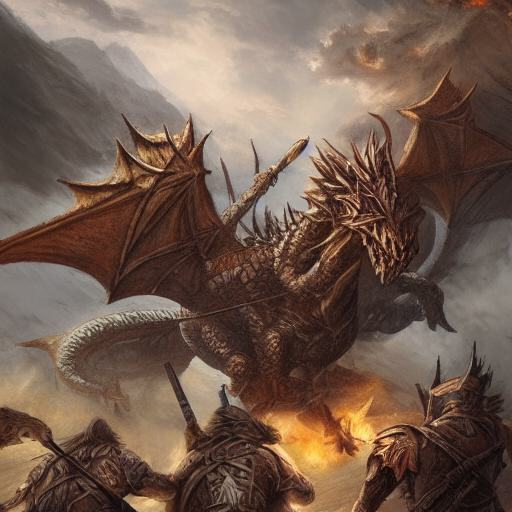
\includegraphics[width=\columnwidth]{introduction/what is a tabletop rpg}
    In tabletop role-playing games like Rise, you play a specific character of your own design.
    Your character can try to do anything you can imagine in a world that the game master, or GM, creates.
    Of course, you won't always succeed.
    The details of your character's capabilities are defined in the pages ahead; when you're done creating a character, it will have a personality of its own, along with strengths, weaknesses, and special abilities.
    Usually, your character will go on adventures with other characters, each of which is played by other players.
    Together, you will create and experience a story with the Game Master, or GM, who defines the universe that the player characters inhabit.

    \subsection{Describing Actions}
        Most of the time, when you're playing a game of Rise, you simply describe what you want your character to do.
        For example, you can say that your character steps out of their room in the inn and walks over to knock on a friend's door.
        Although Rise has rules that could govern some aspects of that scenario, such as an Awareness check to see if your friend notices you knocking, you wouldn't usually reference those rules explicitly.
        Even in the unlikely scenario that your friend doesn't notice you knock the first time, you can just knock again, so there's no point in worrying about the details.
        If something seems reasonable, it probably is, and you don't need to worry about the fiddly bits.

        Sometimes, when you describe what your character tries to do, the action has a narratively relevant chance of failure.
        Instead of knocking on the door to say hi, you might only have time to bang on it once to warn your sleeping friend about an attack from assassins.
        In that case, there's some chance that your friend is sleeping too deeply to notice the noise the first time you knock.
        You could try knocking again, just like in the first scenario, but in this scenario that failure would cost you valuable time to survive the attack.
        In that scenario, you would roll a die to determine whether you succeed in your action - or in this case, whether your friend would succeed in their attempt to notice you.

    \subsection{Using Specific Abilities}
        Instead of describing broadly what you want to have happen, you might choose one of a list of clearly defined abilities that your character can use.
        Every character has specific abilities unique to them, such as a wizard's spells known.
        There are also a number of simple abilities that anyone can use, such as the \ability{dirty trick} or \ability{trip} abilities.
        These universal abilities attempt to adequately describe a wide variety of reasonable improvised actions that you might try to use in combat.

        Explicitly defined abilities have rules for determining what happens when you use them.
        Some abilities, such as attacks in combat, require rolling dice to determine how effective they are.
        Of course, you can use your character's abilities at any time, not just in combat.
        Abilities such as the \spell{create water} or \spell{distant hand} spells can be used to solve other kinds of problems entirely.

    \subsection{Rolling Dice}
        Eventually, you'll have to determine whether something succeeds or fails.
        This can happen as part of using a specific ability that tells you exactly what to roll, or because you tried to narrate your character taking an action that has a dramatically relevant chance of failure.
        In either case, you'll roll a single ten-sided die, also known as 1d10.
        You'll add some modifier that represents how skilled your character is at the particular thing that they are trying to do.
        At the GM's discretion, they may also give the roll an extra bonus or penalty based on the circumstances that your character is in.
        If your die roll is high enough, your character succeeds at whatever they were trying to do.
        Otherwise, your character fails, which may sometimes have additional consequences.

        In Rise, it's entirely possible for characters to be so skilled that they succeed at what they are trying to do even if you roll a 1.
        Likewise, there are tasks that are so obviously impossible for your character that they cannot possibly succeed.
        In those cases, there's no reason to roll!
        Of course, the GM is the final arbiter of whether rolling is necessary.
        They may have information that the players do not.

    \subsection{Why Use So Many Rules?}
        
\includegraphics[width=\columnwidth]{introduction/so many rules}

        Tabletop role-playing games attempt to create rules to define how their universe works.
        Some games are intentionally vague or minimalist about their rules, which can be fun!
        Simple games are easy to start playing, and they try to avoid getting in the way of good role-playing.
        However, Rise takes a different approach.
        It spends a lot of effort - and words - attempting to define an internally consistent universe, and creating a large number of specific abilities that can be used in that universe.
        There are a few important advantages to taking this approach: establishing expectations, supporting multiple play styles, and assisting the GM.

        \subsubsection{Establishing Expectations}
            Different people can have very different ideas about what is realistic - or narratively appropriate - in a made-up fantasy universe.
            To some people, kicking in the tavern door and starting a brawl is just some good clean fun, and you'll take a few good punches and then laugh about it later that evening over drinks.
            But to other people, that might sound like a good way to find yourself imprisoned for the foreseeable future with all of your possessions confiscated by the town guard.
            Another interpretation of that scenario might see the brawler seriously injured with a broken bottle in the eye, leaving them partially blinded for weeks - or indefinitely.

            All of those ideas are valid, and they each match the narrative of a particular type of story.
            However, it's important that everyone sitting at a table and playing a game agrees about what to expect.
            Players can get confused or frustrated when their actions have consequences that feel arbitrary or unfair.
            Generally, games are more fun if everyone in the game shares a common set of expectations and conventions.
            Otherwise, games can devolve into disagreements about what is or isn't reasonable.

            One way to establish these expectations is to use a rules system like Rise that defines some expectations explicitly.
            If the scenario above happened in Rise, the last outcome of an incapacitating bottle to the eye shouldn't normally be possible, since the rules explicitly define how injury works.
            Knowing what is and isn't possible can help give players and GMs a useful set of guardrails for what they try to do in the universe.
            It's relatively easy to get everyone to agree about simple things that regular human people have experience with, like how difficult it is to climb a tree.
            However, Rise is full of superhuman people and monsters, and eventually you'll need to figure out how far a barbarian as strong as Hercules can throw a bear.
            Having a single authoritative resource to consult can cut off long disagreements about details that are difficult or impossible to determine objectively.

            Of course, different games played with a flexible rules system like Rise can have very different tones and themes.
            Either of the first two scenarios in the tavern are still plausible in different games, and a GM can use house rules to make vital wounds have more long-term consequences if they want.
            Using a rules system like Rise can help, but it is not the full answer by itself.
            The GM and players always share responsibility for establishing expectations about what genre a game will be, and conforming to those expectations to the extent that it makes the game more fun.

        \subsubsection{Supporting Multiple Play Styles}
            
\includegraphics[width=\columnwidth]{introduction/multiple play styles}
            Some people deeply enjoy the process of role-playing itself.
            They enjoy the process of getting into a character and speaking in their voice, exploring their needs and desires, and building a narrative for them over time.
            These people often do not need the confines of a robust rules system, and can play equally well in games with minimal rules or none at all.

            Other people do not enjoy role-playing as an end in itself, or even at all.
            However, they may still enjoy the \textit{game} aspect of a role-playing game.
            Instead of playing a character for their personality and backstory, they may play a character for their unique mechanics and tactical advantages.

            Still other people may be interested in role-playing as a concept, but find it daunting.
            The blank page in front of you when you start painting a picture or writing an essay can be daunting, and that first step is often the hardest to take.
            Giving people a clearly defined set of abilities and specific tools for interacting with the world can enhance creativity by providing a safe space for interaction and experimentation.
            Even if you don't enjoy or feel confident in speaking in your character's voice, you can still engage with the narrative aspects of the adventure by casting a relevant spell or making a relevant skill check.
            People in this middle ground can sometimes enjoy deeper role-playing games while being feeling lost in role-playing games with minimal or nonexistent rules.

            One of the joys - and challenges - of Rise is drawing together people with very different desires and play styles to share a single experience.
            Rules-free role-playing games and tactical wargames can both have a narrower appeal than rules-heavy role-playing games like Rise, which try to provide something for everyone.
            You can run games with deep role-players alongside tactical gamers, and it can be a lot of fun.
            It does place a greater burden on the GM to provide the right ratio of content to keep everyone happy, and it does require the players to be patient when their preferred playstyle is put in the background to support the needs of other players.
            A well-blended game can also draw people out of their comfort zones slowly and safely over time as they observe and start to enjoy the playstyles of the other players in the game.

        \subsubsection{Assisting the GM}
            The Game Master carries an extra weight of responsibility to shape the flow of the game.
            Creating narratively consistent universes, appropriate challenges, and engaging storylines out of thin air is deeply challenging.
            If this job is too difficult, no one will want to do it, and then no one will play the game!
            Making the GM's job easier is a critical component of any role-playing game.

            There are several ways that Rise can make the GM's job easier.
            It provides information about the mechanics and tropes of the universe that the game takes place in, which helps establish expectations and resolve disputes that might come up during the game.
            It will provide a clear narrative foundation for the world and the characters in that world, which minimizes the up-front work required to run a game, once that section of the book is more complete.
            It will provide a wealth of pre-packaged challenges appropriate for players of any power level or play style, and advice for how to use those challenges appropriately, once that section of the book is more complete.
            The GM-focused sections are currently the most unfinished part of Rise, and this will be a more useful guide before Rise is done.

\section{What Makes Rise Different?}
    If you haven't played other tabletop role-playing games, feel free to skip this section.
    If you have, you may wonder what makes Rise unique in a crowded sea of games.
    Rise has five fundamental principles that differentiate it from other TTRPGs: minimal resource management, simultaneous combat, optional complexity, unbounded scaling, and a bounded action economy.

    \subsection{Minimal Resource Management}
        Many games make use of resources like mana, spell slots, or timed cooldowns to limit how often characters can use their abilities.
        These systems have fundamental problems that undercut the fun and flow of a TTRPG, and Rise essentially does not use resources to limit character ability usage.
        In Rise, characters can cast spells or use special attacks any number of times in a row without consuming resources.

        Some systems have resources that are designed to ebb and flow in the course of a typical combat.
        You might expend mana to use a powerful spell, and then regain mana over time by using weaker spells or fulfilling certain conditions.
        Alternately, you might use a spell and then wait some number of in-game turns before you can use that same spell again.
        This can be fiddly to track and hard to recover from if you forget what happened to your resource pool, which is why this approach is more common in video games than in TTRPGs.
        More importantly, this system has no clear way to handle ability usage outside of combat.
        It effectively gives unlimited ability usage when time is no obstacle, but only in an awkward and convoluted way.
        This category of system is unsuitable for Rise because it is too fiddly in combat and doesn't make sense out of combat.

        Some systems have finite-use resources that are tied to the expenditure of in-game time, such as taking long rests, or session breaks.
        You might spend a spell slot to use a powerful spell, and then be unable to cast that spell again until your character rests for some period of time.
        This can be manageable from a complexity perspective if the number of unique resources is small.
        However, it can get dangerously convoluted if characters have a large number of separate or partially interchangeable resource pools, such as using separate pools for individual spell levels.

        The real problem is that this limitation requires you to make your decisions based on not just the current situation, but also on your prediction of all future situations you will encounter before you have the opportunity to rest.
        This contributes significantly to the tactical complexity of deciding each individual action in combat, which slows down the pace of the game.
        It is also punishing to newer players who have less experience with the metagaming required to deduce how many resources an individual fight is worth.
        This strategic complexity is compounded if hit points are treated as an additional resource, since you now have to trade off the potential impact of one limited resource against another limited resource.

        Optimization of resource usage can be unintuitive and out of character, but failure to correctly manage your resources can leave you with no useful abilities remaining.
        This concern can be exacerbated if some characters are extremely resource-intensive while others have no meaningful resources to track.
        No one likes being forced to hide from a difficult fight or take only insignificant actions while your more resource-savvy or resource-independent allies continue using dramatic and powerful abilities.
        It can also add stress to the party dynamics when one character frequently asks for long rests after fights because they expended resources and no one else needs to rest.
        This category of system is unsuitable for Rise because it creates complexity in ways that detract from the fun and narrative of a game instead of adding to it.

        Rise does not use resources to limit normal actions in combat.
        The vast majority of spells, special martial attacks, and other abilities that affect enemies or your environment can be used any number of times.
        There are a small number of abilities with one-round cooldowns, and a universal ability that can only be used once per short rest.
        However, there is no time tracking in the system longer than ``next round''.
        Small cooldowns are a fine-grained balancing tool that allow characters to have powerful abilities which would have detrimental effects for the game if they could be used every turn.

        Rise does use a single universal resource, called ``fatigue'', that recovers based on long rests.
        This allows some opportunity for characters to invest extra effort into specific difficult fights, and to become tired after a long day.
        Normal damage taken during a fight is easily recovered after a ten minute rest.
        This means that you typically don't have to track state between fights.
        However, a GM can prevent that rest time with multiple sequential fights to increase difficulty and drama.

        Overall, Rise uses resource limitations very sparingly.
        This allows it to gain some of their benefits while avoiding the detrimental effects that come from making resource limitations a fundamental part of the system.

    \subsection{Simultaneous Combat}
        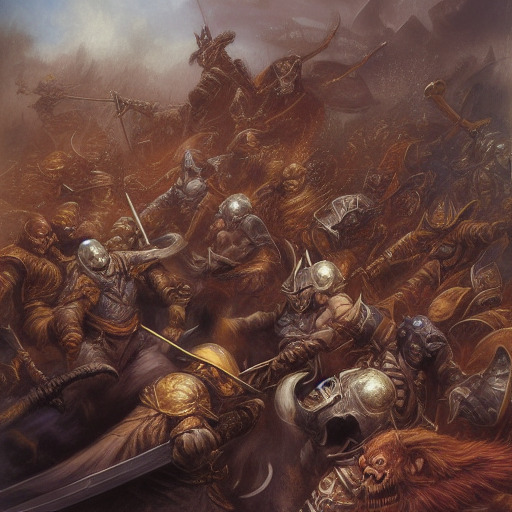
\includegraphics[width=\columnwidth]{introduction/simultaneous combat}
        In most TTRPGs, combat takes place in a series of turns.
        When your turn comes up, you take all of your actions, and then you wait through everyone else's turn until your turn comes again.
        This system has one foundational disadvantage: it is very, very slow.
        Rise uses a simultaneous combat system that dramatically increases the pace of combat.

        Imagine a typical 4-5 player game with 1-2 enemy groups using a traditional turn-based initiative system.
        In this scenario, you have to wait through about 5 turns before it comes back to your turn.
        This number can increase significantly in large-scale fights.
        Each of those 5 or so turns can meaningfully change the battlefield situation on its own by moving, weakening, or defeating various enemies and allies.
        The state of the battlefield at the end of last turn is often drastically different than the state of that battlefield at the start of your new turn.
        Player coordination can be challenging, since they must coordinate in the specific order assigned by the initiative system, and enemy turns can intervene to ruin coordinated plans.

        In theory, every player should accurately track the unfolding battlefield state through each of the intervening turns.
        That would mean everyone would know what to do when their turn comes up.
        In practice, many players find that difficult or impossible.
        Instead, at the start of each of their turns, they ask or try to figure out how the situation has changed.
        Not everyone asks this explicitly, but it must always be analyzed anew.

        Once a player understands the current battlefield state, they can finally decide their actions.
        This typically involves both movement and any number of sequential attacks, so there are many factors to consider.
        Everyone else must wait and do nothing while this happens.
        Once the active player has decided their actions, those actions must be fully rolled and resolved before combat can proceed.
        Even the next player in the initiative order may not be able to make accurate plans during this time, since the die rolls can change those plans.
        All of this combines to make even short combats take an hour or more, and six-person adventuring groups can feel dangerously bloated.

        Rise works differently.
        Combat in Rise is broken up into two phases: the movement phase and the action phase.
        During the movement phase, all creatures move simultaneously, and no attacks are possible.
        Characters can declare certain simple reactive movements like ``stay adjacent to this enemy'' to ensure that they end up in a reasonable position regardless of enemy actions.
        If the movements of characters conflict in impossible ways, initiative checks can temporarily force a linear order of resolution.
        Each player declares their own actions in an arbitrary order as soon as they decide them, so people are not forced to wait and do nothing while slower players contemplate their choices.
        Player coordination is easy, since all actions are happening together.

        During the action phase, players resolve their actions sequentially, but in an arbitrary order of the players' choice.
        This allows slower players to make their decisions when they are ready, while allowing faster players to resolve their actions first.
        Since movement during the action phase is rare, and enemies cannot unexpectedly move, players are typically able to decide their actions much more quickly and easily even when they have a large number of unique abilities to choose from.
        Once all players have resolved their actions, they learn what their enemies did.
        Those actions all resolve simultaneously, so enemy actions cannot interrupt player actions and vice versa.
        Attackers are always responsible for rolling instead of using ``saving throws'' or similar mechanics that force defenders to roll dice.
        All of this means that players can choose and resolve their actions simultaneously and efficiently, minimizing total time spent in combat while still allowing significant tactical complexity.

        The start of each phase still requires a general assessment from all acting players about the current state of the battlefield, which takes just as much time as the assessment in a classic initiative system.
        However, the time required for this tactical analysis only increases marginally as the number of players and enemies in the game increases.
        This allows Rise to handle large player counts or large enemy hordes without becoming glacially slow.
        Combat in Rise flows by quickly, making it much easier to balance time between combat and non-combat encounters within the same game session - or to run through multiple separate, individually challenging combats without sacrificing the pace and energy of the game.

    \subsection{Optional Complexity}
        Many games operate at a consistent level of complexity.
        Many rules-light games are always simple, and many rules-dense games are always complex.
        This is a perfectly reasonable design philosophy.
        Among other benefits, it makes it easy to know what to expect from the game, which helps give the game a well-defined niche.

        Rise is designed to allow players to choose their own level of complexity.
        This broadens its potential audience by allowing people with very different play styles or tolerances for complexity to enjoy the same game together.
        This goal is manifested in several key ways in Rise's design:
        \begin{itemize}
            \item Core gameplay is designed to be simple.
            \item Character creation is deeply interconnected.
            \item Complexity is not tied to narrative roles.
            \item Character power does not require complexity.
        \end{itemize}

        \subsubsection{Simple Core Gameplay}
            The core gameplay loop must be simple.
            You can contribute in combat by relying on one or two standard attacks that you use in all circumstances.
            In narrative situations, you can just roll the skills you have trained, and ignore other options.
            Engaging with the system more deeply than that is a choice, not a requirement.

        \subsubsection{Interconnected Character Creation}
            Character creation and build optimization is a better place to store complexity.
            Creating a Rise character involves a number of decisions, each of which can have nuanced ramifications on other aspects of the system.
            If you are just trying to build a character that matches a desired narrative, you can generally approach each decision in isolation.

            For example, you can decide that your character is intelligent and agile but not very strong or durable, because that is the concept you want.
            That decision has consequences, such as changing how many trained skills you have and what your defenses are.
            If you approach each decision sequentially, each one is relatively easy to make, and doesn't require deep system knowledge.
            On the other hand, trying to mathematically optimize a character requires thinking about many aspects of the system at once.
            This results in a system that is easy to learn but hard to master.

            Even for simple characters, the process of character creation is still one of the most complicated aspects of Rise.
            That is why Rise provides (or will provide, once that section is done) an extensive selection of premade characters for a wide variety of narrative archetypes.
            Each premade character includes advice for how to play that character and level them up.
            The premade characters make the system more accessible to people who don't want to to deal with the complexity of creating a character from scratch.

        \subsubsection{Complexity and Narrative}
            Complexity and simplicity should not be directly connected to a character's concept or narrative.`
            For example, it would be a bad idea to define a system where martial characters are simple and spellcasters are complicated.
            Both of those are rich and evocative narrative constructs.
            Many people who don't enjoy complexity will want to play spellcasters, and many people who enjoy complexity will want to play martial characters.
            Gameplay complexity must be more finely tuned and localized than those sweeping strokes.

            In Rise, gameplay complexity is generally generated by acquiring a large number of increasingly situational abilities.
            Every class has some archetypes that grant additional abilities known and some archetypes that grant additional passive abilities.
            If you like having a lot of unique abilities, you can have a high Intelligence to maximize your insight points, and focus on learning spells and maneuvers that attack your enemies or have situational effects.
            If you like minimizing complexity, you can instead choose archetypes or learn spells that simply grant you passive benefits, and focus on one or two standard attacks that you specialize in.
            Some feats give you new abilities and new circumstances to pay attention to that make you more effective, while others simply increase your passive statistics and defenses.

            Rise specifically handles complexity for martial characters and spellcasters slightly differently.
            Martial characters in Rise typically have fairly simple individual abilities.
            However, they can use those abilities with a variety of meaningfully different weapons.
            A martial character with four unique attacks and three different weapons has twelve different options in combat.
            In addition, martial characters can typically make better use of universal abilities, such as shoving and grappling.

            Spellcasters have more complex and varied individual abilities.
            They also tend to have more abilities that have significant narrative effects.
            However, their abilities are more isolated.
            There is no spellcaster equivalent of martial weapons that would multiply their number of distinct abilities in combat.
            The result of this design is that both martial characters and spellcasters can be very simple or very complicated.
            However, they approach complexity in different ways, ensuring that they feel narratively distinct.

        \subsubsection{Complexity and Power}
            All of this customization of complexity would be mostly pointless if complexity was strongly correlated with character power.
            If exceptionally complicated or hyper-specialized characters were obviously and consistently more effective than other characters, it would push everyone to use those characters.
            Rise structures the tradeoffs between gaining raw power and gaining additional options balanced enough that neither is always superior.

            There will always be some benefit from build optimization and system mastery.
            Players who are deeply familiar with Rise will be able to build characters with more relevant strengths and fewer relevant weaknesses.
            However, the gap between optimized characters and ``normal'' characters is limited.
            There will always be specific contexts where one character's mechanics are superior to another's.
            For example, a specialized defensive melee character may excel in a duel in a confined space.
            However, it may be irrelevant against cavalry archers on an open field.
            Characters in Rise cannot drastically change their capabilities each day, so they will always have moments to shine and moments of weakness.

    \subsection{Unbounded Scaling}
        
\includegraphics[width=\columnwidth]{introduction/unbounded scaling}
        Some systems uses bounded bonuses for accuracy or other game statistics.
        Bounded scaling means that every character of the same power level - or in some systems, of any power level - has a similar chance of success with any given skill check or attack roll.
        This can frequently cause narratively inappropriate and even comical events, and Rise explicitly rejects this philosophy.

        Imagine a typical party of four players, with one character being exceptionally skilled at a particular task.
        Perhaps the rogue is exceptionally skilled at lying, or a barbarian is exceptionally skilled at climbing.
        If ``exceptionally skilled'' only means that they have a \plus5 bonus on a d20 compared to \plus0 from the rest of the party, the exceptionally skilled character will only get the best result in the party half the time.
        The other half of the time, some other character with no relevant skills will meet or exceed the skilled character's result - sometimes by a dramatic margin.
        When failure compared to rank amateurs happens this often, it becomes hard to take seriously the idea that any character can be exceptionally skilled at anything.

        Rise characters can have dramatic statistical differences between each other, even at low levels.
        It uses a d10 as the fundamental die, which makes every bonus more significant.
        In addition, a 1st-level character can easily reach a \plus6 bonus with a skill check that is particularly relevant to their character.
        This means that a skilled character can beat a party of rank amateurs 80\% of the time, and at higher levels their success becomes completely guaranteed.
        Likewise, the difference in Mental defense between a powerful sorcerer and a cowardly rogue can allow mind-affecting attacks to almost always hit a rogue while almost never hitting the sorcerer.
        These statistical differences do not always grow with level, but they remain significant at every level.

        One advantage of systems with bounded scaling is that it is easier to guarantee that every character is relevant in any situation.
        Even if your character has no useful abilities of any kind, you might sometimes succeed on important actions through sheer luck.
        However, this design philosophy often breaks the symmetry between magical and non-magical characters.
        Magical characters can often use extremely specific and powerful abilities that are impossible for nonmagical characters to duplicate.
        If magical characters also have similar odds of success with all generic mechanics of the game, they will almost certainly have far more influence over the narrative of the game than any nonmagical character can hope to match.

        The philosophy of Rise is that it's okay for some characters to be irrelevant in specific contexts.
        It's good to give people time in the spotlight where their character's abilities help solve the specific problem that the group is facing when no other character could.
        Rise encourages that, and makes it impossible for one character to be relevant in \textit{all} contexts.
        Each character has their own strengths and weaknesses, and if you try to be good at everything, you'll fall behind people who specialize in a particular area.
        This will naturally rotate the spotlight between different characters, allowing each player to feel relevant and important in turn.

        This dramatic scaling is also used to govern the power of characters over time, in addition to the power of characters relative to each other.
        Rise attempts to model a massive power range for player characters.
        They are expected to start their journeys at level 1 as little more than commoners, and by level 21 they are effectively demigods who can alter the fate of entire worlds.
        This is a critical part of the narrative fabric of Rise, and it is reflected in the statistics and abilities of characters.
        If a level 1 kobold posed even a tiny threat to a level 21 character, the mechanics of the game would sabotage the purported narrative of power and growth.
        In Rise, overall character power doubles approximately every two to three levels.
        The system takes some care to avoid bloating numbers to unwieldy levels on this journey, and the use of the d10 as the standard die helps immensely.

    \subsection{Bounded Action Economy}
        It is dangerous to to give characters too many actions each turn.
        Each additional action a character can take increases how difficult it is for a player to decide what to do on their turn.
        In addition, each additional action increases the complexity of the change between the start of the turn and the end of the turn.
        This is especially risky with Rise's simultaneous initiative system, which combines the actions taken by all characters into a single resolution process.

        Rise places significant limitations on how many relevant actions each character can take on their turn.
        Generally, characters can only move during the movement phase and then take one significant action each turn.
        Some characters can use a minor action to accomplish something useful.
        However, that essentially marks the end of action economy scaling, even up to the maximum level.

        Detrimental effects that could deny actions are also heavily limited.
        Total action denial effects are only usable by high level characters, and even then they only work against weak enemies or enemies that have already been significantly damaged.
        Taking actions is fun, and sitting quietly while everyone else does things can be very frustrating.
        Similarly, completely removing an enemy's ability to act can easily remove the tension from a fight before it's actually over.


\chapter{Characters}

This chapter describes how individual characters in Rise are defined, including their statistics.
If you plan on playing a premade character, the information in this chapter will still be useful so you can understand how your character works, but you can skip the Character Creation section at the end.
For context about how characters act in combat, see \pcref{Combat}.
For context about how characters act more generally, see \pcref{Adventuring}.

Some of the information in this chapter won't fully make sense until you've read future chapters.
You can either skim past terms you don't yet understand or look them up as you go along.

\section{General Overview}

    \subsection{Species}
        Each character has a species.
        The eight common species are human, dwarf, elf, gnome, half-elf, half-orc, halfling, and orc.
        For details, see \pcref{Species}.

    \subsection{Attributes}
        There are six fundamental attributes: Strength, Dexterity, Constitution, Intelligence, Perception, and Willpower.
        These have broad effects on many aspects of your character's statistics.
        For details, see \pcref{Attributes}.

    \subsection{Combat Statistics}
        There are five main combat statistics: accuracy, defenses, hit points, and damage resistance.
        For details about these statistics are calculated and used, see \pcref{Combat Statistics}.
        \begin{raggeditemize}
            \item Accuracy: This affects how likely you are to hit with attacks.
            \item Damage resistance: This affects how much damage you can shrug off easily.
            \item Defenses: These affects how likely you are to avoid being hit by attacks.
            \item Hit points: This affects how much damage you can take without vital injury.
                Some special abilities have detrimental effects on you if they make you to lose hit points, but not if they only make you lose damage resistance.
            \item Power: This affects how much damage you deal with attacks.
                You have two types of power: \magical power and \glossterm{mundane} power.
        \end{raggeditemize}

    \subsection{Resources}
        There are four main resources: attunement points, encumbrance, fatigue, and insight points.
        For details about these resources are calculated and used, see \pcref{Resources}.
        \begin{raggeditemize}
            \item Attunement points: This affects how many spells and items you can benefit from simultaneously.
            \item Encumbrance: This affects your Strength-based and Dexterity-based checks.
                It typically comes from wearing armor.
            \item Fatigue: This affects your accuracy and checks.
                It typically comes from using special abilities.
            \item Insight points: This affects how many special abilities you know, such as spells and maneuvers.
        \end{raggeditemize}

    \subsection{Size and Weight}
        A character's size category has a variety of implications on their statistics.
        The limits of a character's carrying capacity are similarly measured in similar weight categories.
        For details, see \pcref{Size and Weight}.

    \subsection{Classes}
        Each character has at least one class.
        A character's class has a significant influence on their special abilities and narrative style.
        The eleven classes are briefly summarized below.
        For details about classes, see the Classes chapter, \pref{Classes}.

        \begin{raggeditemize}
            \item Barbarians are primal warriors who draw power from their physical prowess and unfettered emotions.
            \item Clerics are divine spellcasters who draw power from their veneration of a single deity.
            \item Druids are nature spellcasters who draw power from their veneration of the natural world.
            \item Fighters are highly disciplined warriors who excel in physical combat of any kind.
            \item Monks are agile masters of ``ki'' who hone their personal abilities to strike down foes and perform supernatural feats.
            \item Paladins are divinely empowered warriors who exemplify a particular alignment.
            \item Rangers are skilled hunters who bridge the divide between nature and civilization.
            \item Rogues are skillful and versatile characters known for their ability to strike at their foe's weak points in combat.
            \item Sorcerers are arcane spellcasters who draw power from their inherently magical nature.
            \item Warlocks are pact spellcasters who draw their power from a sinister deal made with infernal creatures.
            \item Wizards are arcane spellcasters who study magic to unlock its powerful secrets.
        \end{raggeditemize}

    \subsection{Skills}
        Skills represent the myriad of talents that people can have, such as cooking or swimming.
        Each character is trained in a certain number of skills from their class and Intelligence.

        The twenty-six skills are summarized below.
        For details about skills, see the Skills chapter, \pref{Skills}.

        \begin{raggeditemize}
            \item Awareness: This represents your ability to observe things which you might otherwise fail to notice.
            \item Balance: This represents your ability to maintain your balance and poise in difficult circumstances.
            \item Climb: This represents your ability to climb obstacles.
            \item Craft: This represent your ability to construct objects from raw materials.
            \item Creature Handling: This represents your ability to influence non-sapient creatures.
            \item Deception: This represents your ability to lie or otherwise mislead people without being caught.
            \item Deduction: This represents your ability to make logical deductions based on evidence.
            \item Devices: This represents your ability to to manipulate mechanical devices such as locks, traps, and other contraptions.
            \item Disguise: This represents your ability to create disguises to conceal the appearance of creatures or objects.
            \item Endurance: This represents your ability to persevere through physical trials.
            \item Flexibility: This represents your ability to escape bindings and move through small areas by contorting your body.
            \item Intimidate: This represents your ability to intimidate and coerce people into doing what you want.
            \item Jump: This represents your ability to jump.
            \item Knowledge: This represent your understanding of particular aspects of the world.
            \item Medicine: This represents your practical understanding of how to tend to the wounds of living creatures.
            \item Perform: This represent your ability to create particular forms of entertainment.
            \item Persuasion: This represents your ability to convince people to think what you want them to.
            \item Profession: This represent your practical understanding of a particular profession.
            \item Ride: This represents your ability to ride and control horses and other mounts.
            \item Sleight of Hand: This represents your ability to pick pockets, palm objects, and perform other feats of legerdemain.
            \item Social Insight: This represents your ability to read body language and emotion.
            \item Stealth: This represents your ability to escape detection while moving or taking large-scale actions.
            \item Survival: This represents your ability to take care of yourself and others in the wilderness, including the ability to follow tracks.
            \item Swim: This represents your ability to swim.
        \end{raggeditemize}

\section{Attributes}\label{Attributes}

    Each character has six \glossterm{attributes}: Strength (Str), Dexterity (Dex), Constitution (Con), Intelligence (Int), Perception (Per), and Willpower (Wil).
    These attributes have a wide range of effects on a character's core statistics.

    Each attribute represents a character's raw talent in that area.
    A 0 in an attribute represents average human capability.
    That doesn't mean that every commoner has a 0 in every attribute; not everyone is average, after all.
    Player characters have an average attribute higher than 0 because they are exceptional individuals.

    \subsection{Strength (Str)}\label{Strength}
        {
            Strength measures your muscle and physical power.
            Characters with a high Strength tend to have strong offensive capabilities with nonmagical abilities, and prefer wearing heavier armor.
            It has the following effects:
            \begin{raggeditemize}
                \item Strength determines how much you can carry (see \pcref{Weight Limits}).
                    You generally need a Strength of at least 1 to wear heavy body armor.
                \item You add your Strength to your \glossterm{mundane power} (see \pcref{Power}).
                \item You add your Strength to your level to determine your \glossterm{accuracy} with \abilitytag{Brawling} attacks (see \pcref{Brawling Accuracy}).
                \item A very high Strength can allow you to use \weapontag{Heavy} weapons in one hand (see \pcref{Weapon Tags}).
                \item If your Strength is positive, you reduce your \glossterm{encumbrance} from \glossterm{armor} by an amount equal to your Strength (see \pcref{Encumbrance}).
                \item You add your Strength to Strength-based \glossterm{skills}: Climb, Jump, and Swim (see \pcref{Skills}).
            \end{raggeditemize}
        }

    \subsection{Dexterity (Dex)}\label{Dexterity}
        {
            Dexterity measures your hand-eye coordination, agility, and reflexes.
            Characters with a high Dexterity tend to have strong defensive capabilities, and prefer wearing lighter armor.
            It has the following effects:
            \begin{raggeditemize}
                \item You add your Dexterity to your Armor defense.
                    This bonus can be reduced if you use medium or heavy armor (see \tref{Armor and Shields}).
                \item You add your Dexterity to your Reflex defense.
                \item You add your Dexterity to Dexterity-based \glossterm{skills}: Balance, Flexibility, Ride, Sleight of Hand, and Stealth (see \pcref{Skills}).
            \end{raggeditemize}
        }

    \subsection{Constitution (Con)}\label{Constitution}
        {
            Constitution represents your health and stamina.
            Characters with a high Constitution tend to have strong defensive capabilities.
            It has the following effects:
            \begin{raggeditemize}
                \item Your Constitution increases your \glossterm{hit points}, as defined by your class (see \pcref{Classes}).
                \item You add your Constitution to your \glossterm{fatigue tolerance} (see \pcref{Fatigue}).
                \item You add your Constitution to your Fortitude defense.
                \item You add your Constitution to the Constitution-based \glossterm{skill}: Endurance (see \pcref{Skills}).
            \end{raggeditemize}
        }

    \subsection{Intelligence (Int)}\label{Intelligence}
        {
            Intelligence represents how well you learn and reason.
            Characters with a high Intelligence tend to have more options and special abilities.
            It has the following effects:

            \begin{raggeditemize}
                \item If your Intelligence is positive, you gain a number of \glossterm{trained skills} equal to your Intelligence (see \pcref{Trained Skills}).
                \item You add your Intelligence to the number of \glossterm{insight points} you gain (see \pcref{Insight Points}).
                \item You add your Intelligence to Intelligence-based \glossterm{skills}: Craft, Deduction, Disguise, Knowledge, and Medicine (see \pcref{Skills}).
            \end{raggeditemize}

            \par Creatures incapable of complex cognition and speech, like animals, have an Intelligence of \minus6 or lower.
            Creatures capable of speech have an Intelligence of at least \minus5.
        }

    \subsection{Perception (Per)}\label{Perception}
        {
            Perception describes your ability to observe and be aware of your surroundings.
            Characters with a high Perception tend to have strong offensive capabilities.
            It has the following effects:
            \begin{raggeditemize}
                \item You add your Perception to your level to determine your \glossterm{accuracy} with almost all attacks (see \pcref{Accuracy}).
                \item You add your Perception to Perception-based \glossterm{skills}: Awareness, Creature Handling, Social Insight, and Survival (see \pcref{Skills}).
            \end{raggeditemize}
        }

    \subsection{Willpower (Wil)}\label{Willpower}
        {
            Willpower represents your ability to endure mental hardships.
            Characters with a high Willpower tend to be better at attacking with and defending against magical abilities.
            It has the following effects:
            \begin{raggeditemize}
                \item You add your Willpower to your \glossterm{magical power} (see \pcref{Power}).
                \item You add your Willpower to your Mental defense.
            \end{raggeditemize}
        }

\section{Species}\label{Species}
    Each character has a species.
    There are seven common species described below.
    At the GM's discretion, you may be able to play a character with a more unusual species (see \pcref{Uncommon Species}).

    \subsection{Humans}
        
\includegraphics[width=\columnwidth]{characters/human}

        Humans are the most common and least rigidly defined of all Rise species.
        They are not the smartest, the strongest, or the most durable of the civilized races.
        They have no supernatural senses or impossible talents; anything a human can do, a member of another species could do at least as well.
        Despite their limitations, humans are practically universal, and their civilizations are the most powerful and numerous of all.

        The success of humanity comes from one core strength: their adaptability, both individually and as a whole.
        Individual humans can learn new skills with surprising ease compared to other species, and they often have a breadth of talent that few can rival.
        The relatively short human lifespan prevents their society from stagnating under the guidance of elders whose wisdom is now hundreds of years out of date.
        When radical changes sweep the world, humans can adapt where other species would founder.

        \parhead{Size} Medium.
        \parhead{Attributes} See the Versatile ability.
        \parhead{Special Abilities}
        \begin{raggeditemize}
            \itemhead{Skilled} Humans gain an additional \glossterm{trained skill} (see \pcref{Skills}).
            \itemhead{Versatile} Humans gain a \plus1 bonus to any attribute.
                This cannot increase that attribute above 4 when attributes are initially determined (see \pcref{Attributes}).
                That attribute can later be increased above 4, such as by the attribute bonus at level 3 (see \pcref{Character Advancement and Gaining Levels}).
        \end{raggeditemize}
        \parhead{Automatic Language} Common, any two \glossterm{common languages} or one \glossterm{rare language} (see \pcref{Communication and Languages}).

    \subsection{Dwarves}
        
\includegraphics[width=\columnwidth]{characters/dwarf}

        Dwarves are short, stout, and sturdy.
        It has been said that the first dwarf was carved from stone, and the similarities have been noted by many.
        All dwarves naturally have beards, and the vast majority keep them long and elegantly maintained.

        Most dwarves live underground in mining communities.
        These communities can grow to massive size, and dwarven kings can rule vast underground cities.
        The dwarven fascination with strong drink is legendary, though somewhat misleading.
        Their natural resilience means they need stronger drinks to even notice the effects, so other species tend to gain an exaggerated impression of dwarven drunkenness when they try to drink dwarven ale.

        \parhead{Size} Medium.
        \parhead{Attributes} \plus1 Constitution, \plus1 Willpower, \minus1 Dexterity.
        \parhead{Special Abilities}
        \begin{raggeditemize}
            \itemhead{Darkvision} Dwarves have \trait{darkvision} with a 60 foot range, allowing them to see in complete darkness (see \pcref{Darkvision}).
            \itemhead{Depth Sense} Dwarves can intuitively sense their approximate depth underground as naturally as a human can sense which way is up.
            \itemhead{Earthen Crafting} Dwarves gain a \plus2 bonus to the Craft (metal) and Craft (stone) skills.
            \itemhead{Slow and Steady} Dwarves have a \minus10 foot penalty to their speed with all \glossterm{movement modes}.
                However, wearing heavy \glossterm{body armor} does not reduce a dwarf's speed (see \pcref{Armor Usage Classes}).
                In addition, a dwarf's land speed cannot be more than 10 feet slower than their \glossterm{base speed}, even while \slowed or under similar effects.
                This does not affect movement through \glossterm{difficult terrain} and similar effects, since those affect movement cost rather than your character's intrinsic movement speed.
        \end{raggeditemize}
        \parhead{Automatic Languages} Common, Dwarven, any one \glossterm{common language} (see \tref{Common Languages}).

    \subsection{Elves}
        
\includegraphics[width=\columnwidth]{characters/elf}

        Elves are tall, lithe, and graceful.
        They tend to have an air of confidence at all times, and even their mistakes seem intentional.
        Elves have the longest lifespan of any civilized species, and even comparatively young elves carry a weight of experience that can be daunting for non-elves.

        For millenia, elves were the most powerful civilization above ground, while dwarves claimed the underground.
        More recently, humans have usurped elves as the most powerful civilization above ground, while dwarves have kept their claim.
        This history, combined with their natural differences, has created an ancient rivalry between elves and dwarves that sometimes manifests as outright hatred.

        \parhead{Size} Medium.
        \parhead{Attributes} \minus1 Constitution, either \plus1 Dexterity or \plus1 Perception.
        \parhead{Special Abilities}
        \begin{raggeditemize}
            \itemhead{Elven Serenity} Elves gain a \plus1 bonus to Mental defense.
            \itemhead{Keen Senses} Elves gain a \plus2 bonus to the Awareness skill (see \pcref{Awareness}).
            \itemhead{Low-light Vision} Elves have \trait{low-light vision}, allowing them to see clearly in \glossterm{shadowy illumination} (see \pcref{Low-light Vision}).
            \itemhead{Sure-Footed} Elves gain a \plus2 bonus to the Balance and Stealth skills (see \pcref{Balance}, and \pcref{Stealth}).
            \itemhead{Trance} Elves do not sleep, and are immune to \magical effects that would cause them to sleep.
                Instead of sleeping, elves can trance for 4 hours.
                An elf in trance may make Perception-based checks at a \minus5 penalty.
                Elves must still avoid strenuous activity for 8 hours to heal and gain other benefits of taking a \glossterm{long rest}.
        \end{raggeditemize}
        \parhead{Automatic Languages} Common, Elven, any one \glossterm{common language} (see \tref{Common Languages}).

    \subsection{Gnomes}
        
\includegraphics[width=\columnwidth]{characters/gnome}

        Gnomes are the smallest, most magical, and most short-lived of the civilized species.
        Their large eyes and heads give even adult gnomes almost child-like proportions.
        Fae blood runs in the blood of all gnomes, and gnome societies have many traditions and rituals that seem superstitious to outsiders.
        However, these rituals have a purpose, and gnomes understand that failing to appease the hidden powers in the world can have dangerous consequences.

        Most gnomes live in forests, but they can be found in remote areas all over the world.
        Gnomish settlements are almost always overseen by minor fae, such as dryads, who protect the settlement.
        In many cases, the settlements were originally built around a site of mystic power, though some settlements have outlived their original protectors.

        \parhead{Size} Medium.
        \parhead{Attributes} \minus1 Strength, either \plus1 Constitution or \plus1 Intelligence.
        \parhead{Special Abilities}
        \begin{raggeditemize}
            \itemhead{Fae Light}[\sparkle] A gnome can use the \textit{fae light} ability as a standard action.
                \begin{activeability}{Fae Light}
                    \rankline
                    A Tiny glowing orb appears at a location within \rngmed range.
                    It sheds pale, \glossterm{bright illumination} in a \areasmall radius, and \glossterm{shadowy illumination} in a \areamed radius.
                    The orb is intangible, and cannot be moved once placed.

                    This ability lasts until you use it again or until you \glossterm{dismiss} it as a free action.
                \end{activeability}
            \itemhead{Magic Affinity} Gnomes gain an additional \glossterm{insight point}.
                They can only spend this insight point to learn \magical abilities, such as spells.
            \itemhead{Short Stature} Gnomes gain a \plus3 bonus to the Stealth skill.
            \itemhead{Tinkerer} Gnomes gain a \plus2 bonus to one Craft skill of their choice (see \pcref{Craft}).
        \end{raggeditemize}
        \parhead{Automatic Languages} Common, Gnome, either Sylvan or any one \glossterm{common language} (see \tref{Common Languages}).

    \subsection{Half-Elves}\label{Half-Elves}
        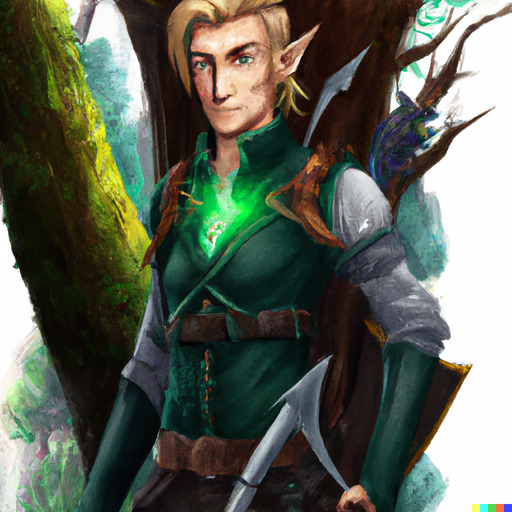
\includegraphics[width=\columnwidth]{characters/halfelf}

        Half-elves carry both human and elven heritage.
        They are caught between two worlds, with neither the unconscious grace of elves nor the limitless adaptability of humans.
        However, they have their own unique forms of versatility based on their understanding of both worlds.

        \parhead{Size} Medium.
        \parhead{Attributes} No change.
        \parhead{Special Abilities}
        \begin{raggeditemize}
            \itemhead{Diplomatic} Half-elves gain a \plus2 bonus to the Persuasion skill.
            \itemhead{Keen Senses} Half-elves gain a \plus2 bonus to the Awareness skill (see \pcref{Awareness}).
            \itemhead{Low-light Vision} Half-elves have \trait{low-light vision}, allowing them to see clearly in \glossterm{shadowy illumination} (see \pcref{Low-light Vision}).
            \itemhead{Versatile} Half-elves only need to spend one \glossterm{insight point} to gain access to an additional class (see \pcref{Multiclass Characters}).
        \end{raggeditemize}
        \parhead{Automatic Language} Common, Elven, any two \glossterm{common languages} or one \glossterm{rare language} (see \pcref{Communication and Languages}).

    \subsection{Half-orc}
        
\includegraphics[width=\columnwidth]{characters/halforc}

        Half-orcs carry both human and orcish heritage.
        They have much of the brute strength of orcs, but tempered by human adaptability.
        While half-elves are often welcome in both human and elvish societies, half-orcs tend to face more challenges navigating both human and orc societies.

        \parhead{Size} Medium.
        \parhead{Attributes} \plus1 Strength, either \minus1 Intelligence or \minus1 Perception.
        \parhead{Special Abilities}
        \begin{raggeditemize}
            \itemhead{Darkvision} Half-orcs have \trait{darkvision} with a 60 foot range, allowing them to see in complete darkness (see \pcref{Darkvision}).
            \itemhead{Intimidating} Half-orcs gain a \plus2 bonus to the Intimidate skill (see \pcref{Intimidate}).
            \itemhead{Physical Instincts} Half-orcs gain an additional \glossterm{insight point}.
                They can only spend this insight point to learn \glossterm{mundane} abilities, such as combat styles and maneuvers.
        \end{raggeditemize}
        \parhead{Automatic Languages} Common, Orcish, any one \glossterm{common language}.

    \subsection{Halflings}
        
\includegraphics[width=\columnwidth]{characters/halfling}

        Halflings stand at about half the height of a human, but have generally human-like proportions.
        They tend to be plucky, adventurous, and outgoing.
        Of all species, halflings have the fewest halfling-only communities.
        Instead, halfling groups tend to live in the gaps between the ``big people'', especially in large cities.

        \parhead{Size} Medium.
        \parhead{Attributes} \minus1 Strength, either \plus1 Dexterity or \plus1 Willpower.
        \parhead{Special Abilities}
        \begin{raggeditemize}
            \itemhead{Nimble Combatant} Halflings gain a \plus1 bonus to Reflex defense.
            \itemhead{Short Stature} Halflings gain a \plus3 bonus to the Stealth skill.
            \itemhead{Stout-Hearted} Halflings gain a \plus1 bonus to Mental defense.
            \itemhead{Sure-Footed} Halflings gain a \plus2 bonus to the Balance skill (see \pcref{Balance}).
        \end{raggeditemize}
        \parhead{Automatic Languages} Common, Halfling, any one \glossterm{common language} (see \tref{Common Languages}).

    \subsection{Orcs}
        
\includegraphics[width=\columnwidth]{characters/halforc}

        Orcs are tall, physically imposing green-skinned humanoids with a reputation for brutishness.
        The orcs that interact with human civilization must content with prejudice, especially in rural areas.
        This is partially inspired by their less civilized cousins who live in more violent environments, and partially a simple reaction to their raw physical presence.

        \parhead{Size} Medium.
        \parhead{Attributes} \plus1 Strength, \minus1 Intelligence, \minus1 Perception, either \plus1 Dexterity or \plus1 Constitution.
        \parhead{Special Abilities}
        \begin{raggeditemize}
            \itemhead{Darkvision} Orcs have \trait{darkvision} with a 60 foot range, allowing them to see in complete darkness (see \pcref{Darkvision}).
            \itemhead{Intimidating} Orcs gain a \plus3 bonus to the Intimidate skill (see \pcref{Intimidate}).
            \itemhead{Raw Strength} Orcs gain a \plus1 bonus to their Strength for the purpose of determining their \glossterm{weight limits} (see \pcref{Weight Limits}).
        \end{raggeditemize}
        \parhead{Automatic Languages} Common, Orcish.

\section{Combat Statistics}

    \subsection{Accuracy}\label{Accuracy}
        Your accuracy with an \glossterm{attack} is the number that you add to the \glossterm{attack roll} (see \pcref{Attack Rolls}).
        Your accuracy is equal to half the sum of your level and Perception.
        Many abilities can also modify your accuracy.

        \subsubsection{Brawling Accuracy}\label{Brawling Accuracy}
            Some abilities have the \abilitytag{Brawling} tag.
            Your accuracy with those abilities is equal to half the sum of your level and Strength.
            Most Brawling abilities are listed at \pcref{Special Combat Abilities}.

    \subsection{Damage Resistance}\label{Damage Resistance}
        Your \glossterm{damage resistance} measures how much damage you can shrug off without any effects.
        For details about how damage resistance is used, see \pcref{Taking Damage}.

        You do not intrinsically have any damage resistance.
        Wearing armor can significantly increase your damage resistance (see \pcref{Armor}).
        In addition, some class abilities and magic items can also increase it.

    \subsection{Defenses}\label{Defenses}
        When you are attacked, your defenses determine the value that the attacker needs to get on the attack roll in order to hit you (see \pcref{Attack Rolls}).
        The four defenses are described below.
        \begin{itemize}
            \item Armor defense (AD): Your Armor defense protects you from normal physical attacks, such as attempts to hit you with a sword.
                It is the most commonly used defense.
            \item Reflex defense: Your Reflex protects you from physical attacks that armor does not help against, such as pit traps or bolts of lightning.
            \item Fortitude defense: Your Fortitude defense protects you from attacks you have to physically endure or resist, such as poisons and life-draining spells.
            \item Mental defense: Your Mental defense protects you from attacks you have to mentally endure or resist, such as terrifying creatures and magical mind manipulation.
        \end{itemize}

        Your defenses are calculated in the following way:
        \begin{itemize}
            \itemhead{Armor} Half level \add Dexterity (modified depending on equipped armor) \add defense bonuses from equipped body armor and shield
            \itemhead{Fortitude} Half level \add Constitution \add class defense bonus
            \itemhead{Reflex} Half level \add Dexterity \add class defense bonus
            \itemhead{Mental} Half level \add Willpower \add class defense bonus
        \end{itemize}
        Each defense may also have various bonuses or penalties applied by special abilities.

    \subsection{Hit Points}\label{Hit Points}
        Your \glossterm{hit points} measure how hard you are to seriously injure or kill.
        For details about how hit points are used, see \pcref{Taking Damage}.

        The way you calculate your hit points is defined by your class (see \pcref{Classes}).
        Increasing your level and Constitution will increase your hit points.

        \parhead{What Hit Points Represent} Hit points represent a combination of durability, luck, divine providence, and sheer determination, depending on the nature of the creature being damaged.
        When lose hit points from an orc with a greataxe, the axe did not literally carve into your skin without affecting your ability to fight.
        Instead, you avoided the worst of the blow, but it bruised you through your armor, the effort to dodge the blow fatigued you, or it barely nicked you through sheer luck -- and everyone's luck runs out eventually.

    \subsection{Power}\label{Power}
        Your \glossterm{power} is a general representation of how strong your abilities are.
        You have two types of power: your \glossterm{magical power}, which affects your \magical abilities, and your \glossterm{mundane power}, which affects your \glossterm{mundane} abilities.
        If you gain a bonus to your \glossterm{power}, and it does not specify which type of power it affects, it affects both your \glossterm{magical power} and your \glossterm{mundane power}.

        Your mundane power is equal to your Strength \add half your level.
        Similarly, your magical power is equal to your Willpower \add half your level.
        If this total is negative, you subtract that value from the damage you deal, ignoring the stated power scaling on the ability.
        For example, a strike with a broadsword would normally deal 1d6 damage \plus1 per 2 power.
        A level 1 character with a \minus2 Strength would deal 1d6 \sub 2 damage, to a minimum of 0.

        Many abilities have stronger effects depending on your \glossterm{power}, especially damaging abilities.
        % TODO: weapon damage wording
        For example, you gain a \plus1 bonus to your \glossterm{weapon damage} for every 2 power you have (see \pcref{Strikes}).

\section{Resources}\label{Resources}

    \subsection{Attunement Points}\label{Attunement Points}
        Many special abilities and magic items only function as long as a creature attunes to them.
        For details, see Attunement, below.

        Your \glossterm{class} gives you a certain number of attunement points.
        You gain additional attunement points as you gain levels (see \pcref{Character Advancement and Gaining Levels}).
        A small number of abilities can also grant additional \glossterm{attunement points}.

        \subsubsection{Attunement}\label{Attunement}
            Abilities that require attunement to function have the \abilitytag{Attune} tag.
            Attuning to an ability typically require investing a single \glossterm{attunement point}.
            You can release your attunement to an effect as a \glossterm{free action}, which typically ends the effect completely.
            This allows you to use that attunement point to attune to a different effect.
            You can never attune to the same ability more than once.

            Normally, the creature using the attuned ability must attune to it.
            In the special case of \glossterm{rituals}, any number of ritual participants can attune to the ability, and the ability lasts as long as any participant is still attuned to it.
            There are two special subtypes of attunement abilities: deep attunements and targeted attunements.

            \parhead{Deep Attunement} This ability require investing two attunement points instead of only one.
            In addition, releasing a deep attunement does not immediately return the invested attunement points.
            Instead, they only return after you finish a \glossterm{short rest}.
            Deep attunements are identified as \abilitytag{Attune} (deep).

            \parhead{Targeted Attunement} This ability requires attunement from the target instead of the creature using the ability.
            If it targets multiple creatures, each target must attune to its own version of the effect.
            When a target releases its attunement, the effect only ends for it, not for any other targets.
            Targeted attunements are identified as \abilitytag{Attune} (target).

    \subsection{Encumbrance}\label{Encumbrance}
        Your encumbrance is a value that represents how much you are burdened by your armor (see \pcref{Armor}).
        You apply your encumbrance as a penalty to all Strength-based and Dexterity-based checks you make.
        If your Strength is positive, you reduce your encumbrance by an amount equal to your Strength.
        This cannot reduce your encumbrance below 0.

    \subsection{Fatigue}\label{Fatigue}
        Thoughout the day, you can become fatigued by your exertions both in and out of combat.
        While \glossterm{hit points} are easy to restore, reducing your \glossterm{fatigue level} generally requires a \glossterm{long rest}.
        Fatigue is still easier to recover from than \glossterm{vital wounds}.

        \subsubsection{Fatigue Level}\label{Fatigue Level}
            Your \glossterm{fatigue level} measures how fatigued you are.
            A number of abilities and attacks can cause you to increase your fatigue level.
            The most common abilities that increase your fatigue level are the \textit{desperate exertion}, \textit{recover}, and \textit{sprint} abilities.
            All of those abilities are described in \pcref{Universal Abilities}.

        \subsubsection{Fatigue Tolerance}\label{Fatigue Tolerance}
            Becoming slightly fatigued is not immediately detrimental.
            Your fatigue level can be as high as your Constitution without suffering any consequences (minimum 0).
            This value is called your \glossterm{fatigue tolerance}.
            Your \glossterm{class} gives you a bonus to your fatigue tolerance, and some abilities can also modify it.

        \subsubsection{Fatigue Penalty}\label{Fatigue Penalty}
            You take a penalty to \glossterm{accuracy} and \glossterm{checks} equal your \glossterm{fatigue level} \sub your \glossterm{fatigue tolerance} (minimum 0).
            This penalty is called your \glossterm{fatigue penalty}.

        \subsubsection{Exhaustion}\label{Exhaustion}
            When your \glossterm{fatigue penalty} reaches \minus5, you fall \unconscious until your fatigue penalty is reduced below \minus5.
            Generally, this means that you are unconscious for 8 hours.

        \subsubsection{Recovering From Fatigue}
            When you finish a \glossterm{long rest}, your \glossterm{fatigue level} is restored to 0 (see \pcref{Resting}).
            There are no other ways to reduce your fatigue level.

    \subsection{Insight Points}\label{Insight Points}
        You can spend \glossterm{insight points} to gain new special abilities.
        Your \glossterm{class} gives you a certain number of insight points, and you gain a bonus (or penalty) to that number of insight points equal to your Intelligence.
        You gain additional attunement points as you gain levels (see \pcref{Character Advancement and Gaining Levels}).
        Some abilities can also grant insight points.
        
        You can spend two \glossterm{insight points} to become a \glossterm{multiclass} character (see \pcref{Multiclass Characters}).
        In addition, every class has at least one way to spend \glossterm{insight points} to learn additional abilities.
        These options are listed below.
        \begin{itemize}
            \item Barbarian: Combat styles, exotic weapons, and maneuvers
            \item Cleric: Mystic spheres and spells
            \item Druid: Mystic spheres, spells, and wild aspects
            \item Fighter: Battle tactics, combat styles, and maneuvers
            \item Fighter: Combat styles, ki manifestations, and maneuvers
            \item Paladin: Mystic spheres and spells
            \item Ranger: Combat styles, hunting styles, and maneuvers
            \item Rogue: Bardic performances, combat styles, maneuvers, and trained skills
            \item Sorcerer: Mystic spheres and spells
            \item Warlock: Mystic spheres and spells
            \item Wizard: Metamagic, mystic spheres, and spells
        \end{itemize}

\section{Size and Weight}\label{Size and Weight}

    \subsection{Size Categories}\label{Size Categories}
        Your size affects your \glossterm{space} in combat, your speed with any \glossterm{movement modes} that depend on your size category's \glossterm{base speed}, your attributes, and how noticeable you are (see \pcref{Stealth}).
        These effects are shown on \trefnp{Size Categories}.
        Size categories are also relevant for determining weight (see \pcref{Weight Limits}).

        \begin{dtable*}
            \lcaption{Size Categories}
            \begin{dtabularx}{\textwidth}{l l l l l l l X}
                \tb{Size}   & \tb{Space}\fn{1} & \tb{Base Speed} & \tb{Weight Limits}\fn{2} & \tb{Reflex} & \tb{Stealth} & \tb{Weapons}             & \tb{Example Creature} \tableheaderrule
                Fine        & 1/4 ft.          & 10 ft.          & \minus4 Str              & \plus4      & \plus20      & \tdash                   & Fly                   \\
                Diminuitive & 1/2 ft.          & 10 ft.          & \minus3 Str              & \plus3      & \plus15      & \tdash                   & Mouse                 \\
                Tiny        & 1 ft.            & 20 ft.          & \minus2 Str              & \plus2      & \plus10      & \tdash                   & Rat                   \\
                Small       & 2-1/2 ft.        & 20 ft.          & \minus1 Str              & \plus1      & \plus5       & \tdash                   & Cat                   \\
                Medium      & 5 ft.            & 30 ft.          & \tdash                   & \tdash      & \tdash       & \tdash                   & Human                 \\
                Large       & 10 ft.           & 40 ft.          & \plus1 Str               & \minus1     & \minus5      & \tdash                   & Ogre                  \\
                Huge        & 20 ft.           & 50 ft.          & \plus2 Str               & \minus2     & \minus10     & \weapontag{Massive} (10) & Hill giant            \\
                Gargantuan  & 40 ft.           & 60 ft.          & \plus3 Str               & \minus3     & \minus15     & \weapontag{Massive} (15) & Roc                   \\
                Colossal    & 80\add ft.       & 80 ft.          & \plus4 Str               & \minus4     & \minus20     & \weapontag{Massive} (20) & Great wyrm red dragon \\
            \end{dtabularx}
            1 Creatures can vary in space. These are simply typical values. \\
            2 This modifies Strength only for the purpose of determining a creature's \glossterm{weight limits} (see \pcref{Weight Limits}). \\
        \end{dtable*}

        \subsubsection{Space}\label{Space}
            A creature's \glossterm{space} is the area its body occupies while fighting.
            All humanoid species take up a 5-ft.\ by 5-ft.\ space in combat, which is a single \glossterm{square}.
            Normally, other creatures can't be in the space you occupy.
            Most creatures have a space significantly larger than the physical space their body occupies because they need room to maneuver in combat.

            Exceptionally large creatures can often attack at some distance from their core body thanks to long arms or other appendages.
            This is represented by making their space larger than their body alone would require.
            Even Colossal creatures can still only make melee attacks against adjacent foes - or more often, against smaller creatures sharing space with them.

        \subsubsection{Base Speed}\label{Base Speed}
            Each size category has a \glossterm{base speed} that indicates how far creatures of that size category can generally move.
            Most \glossterm{movement modes} use a speed equal to the base speed for a creature's size category.
            For context about movement in combat, see \pcref{Movement and Positioning}.

        \subsubsection{Other Effects}
            % TODO: record all of these and add them here
            A creature's size affects some additional skills and abilities.
            For example, larger creatures have a penalty to the Stealth skill (see \pcref{Common Stealth Modifiers}).
            The effects of unusual size are described in those skills and abilities.
            Unusually large or small creatures also have other special rules apply to them, as described below.

        \subsubsection{Very Small Creatures}
            \parhead{Space} If a creature takes up less than a single square of space, you can fit multiple creatures in that square.
            Ignoring flight, you can fit four Small creatures in a square, twenty-five Tiny creatures, 100 Diminuitive creatures, or 400 Fine creatures.
            If the creatures can fly, the number of creatures that can fit into a space increases drastically.

            \parhead{Movement} Creatures two size categories smaller than you are not considered obstacles and do not hinder your movement.

        \subsubsection{Very Large Creatures}\label{Very Large Creatures}
            \parhead{Space} Very large creatures take up multiple squares. Anything which affects a single square the creature occupies affects the creature.

            \parhead{Movement} Creatures two size categories larger than you are not considered obstacles and do not hinder your movement.

            \parhead{Massive Weapons} Creatures that are Huge or larger have \weapontag{Massive} weapons, as shown in \trefnp{Size Categories}.

    \subsection{Weight Limits}\label{Weight Limits}

        \begin{dtable}
            \lcaption{Weight Limits by Strength}
            \setlength{\tabcolsep}{4pt}
            \begin{dtabularx}{\columnwidth}{X X X}
                \tb{Strength} & \tb{Carrying Capacity} & \tb{Push/Drag} \tableheaderrule
                -9            & Fine x8                & Tiny          \\
                -8            & Diminuitive x2         & Tiny x2       \\
                -7            & Diminuitive x4         & Tiny x4       \\
                -6            & Diminuitive x8         & Tiny x8       \\
                -5            & Tiny x2                & Small x2      \\
                -4            & Tiny x4                & Small x4      \\
                -3            & Tiny x8                & Small x8      \\
                -2            & Small x2               & Medium x2     \\
                -1            & Small x4               & Medium x4     \\
                0             & Small x8               & Medium x8     \\
                1             & Medium x2              & Large x2      \\
                2             & Medium x4              & Large x4      \\
                3             & Medium x8              & Large x8      \\
                4             & Large x2               & Huge x2       \\
                5             & Large x4               & Huge x4       \\
                6             & Large x8               & Huge x8       \\
                7             & Huge x2                & Gargantuan x2 \\
                8             & Huge x4                & Gargantuan x4 \\
                9             & Huge x8                & Gargantuan x8 \\
                10            & Gargantuan x2          & Colossal x2   \\
                11            & Gargantuan x4          & Colossal x4   \\
                12            & Gargantuan x8          & Colossal x8   \\
                13            & Colossal x2            & Colossal x16  \\
                14\plus\fn{1} & \tdash                 & \tdash        \\
            \end{dtabularx}
            1 To calculate the weight limits for a creature with epic Strength, double the number of objects it can carry and drag for every point of Strength beyond 13.
        \end{dtable}

        Your Strength determines how much you can carry or push, as shown in \trefnp{Weight Limits by Strength}.
        Your weight limits are measured in terms of how many objects or creatures of a given \glossterm{weight category} that you can carry or push at once (see \pcref{Weight Categories}).
        The limit of how much you can hold in your hands or on your body is called your \glossterm{carrying capacity}.
        If you need to move more weight than that, you can push or drag objects or creatures up your pushing and dragging limit as a standard action.
        When you do, you move the weight 5 feet.

        In general, it is not meaningful to consider the weight of any objects with a weight category lighter than your maximum weight category.
        If it matters, you can treat eight objects of one weight category as having an equivalent weight to a single object that is one weight category heavier.

        \parhead{Large Creatures} Unusually large or small creatures gain a bonus to their Strength for the purpose of determining their weight limits.
        For details, see \tref{Size Categories}.

        \parhead{Multi-Legged Creatures} The figures on \trefnp{Weight Limits by Strength} are for bipedal creatures.
        A creature with four or more legs can carry, push, or drag twice as many objects as a bipedal creature of the same Strength.

        \subsubsection{Weight Categories}\label{Weight Categories}
            Weight is generally measured in \glossterm{weight categories} rather than pounds or kilograms.
            Weight categories use the same terms as \glossterm{size categories}, as shown in \tref{Weight Categories}.
            In general, a creature's weight category is the same as its size category.

            Objects and creatures can also be either \glossterm{lightweight} or \glossterm{heavyweight}.
            Lightweight objects and creatures have a weight category that is one category lighter than their size category.
            Heavyweight objects and creatures have a weight category that is one category heavier than their size category.

            Objects that occupy only a small percentage of the space appropriate for their size category, such as swords, are usually lightweight.
            Objects that fully occupy the space appropriate for their size category, like boulders, are usually heavyweight.

            \begin{dtable}
                \lcaption{Weight Categories}
                \begin{dtabularx}{\textwidth}{l X}
                    \tb{Weight Category} & \tb{Average Weight} \tableheaderrule
                    Fine        & 1 oz.       \\
                    Diminuitive & 1/2 lb.     \\
                    Tiny        & 2 lb.       \\
                    Small       & 15 lb.      \\
                    Medium      & 125 lb.     \\
                    Large       & 1,000 lb.   \\
                    Huge        & 8,000 lb.   \\
                    Gargantuan  & 64,000 lb.  \\
                    Colossal    & 512,000 lb. \\
                \end{dtabularx}
            \end{dtable}

\section{Calculation Guidelines}
    This explains some general guidelines to follow when calculating character statistics.

    \subsection{Stacking Rules}\label{Stacking Rules}
        Usually, modifiers stack with each other, meaning that you add or subtract all of the modifiers to get the final result.
        However, some modifiers do not stack with each other, as described below.
        When bonuses don't stack with each other, you only apply the largest bonus.
        Likewise, when penalties don't stack with each ather, you only apply the largest penalty.

        \parhead{Special Exceptions}

        \begin{itemize}
            \item Effects from the same source do not stack. Any ability with the same name has the same source.
            \item Enhancement bonuses do not stack with each other.
            \item If a creature gains the same condition multiple times, the effects do not stack, but each instance of the condition is tracked separately.
                The creature must remove all instances of the condition before the effects are removed.
            \item Multiple \magical effects that change a creature's \glossterm{size category} do not stack.
                If multiple magical effects both increase and decrease size, size increases offset size decreases on a one-for-one basis to determine the creature's final size.
            \item If you have two separate abilities which grant you a special sense with a particular range, such as \trait{darkvision} or \trait{blindsight}, you sum the range from both abilities to find your total range with that sense.
        \end{itemize}

    \subsection{Minimum and Maximum Modifiers}\label{Minimum and Maximum Modifiers}
        Some bonuses specify that they cannot increase the value beyond a given point.
        These bonuses must always be applied last, and cannot be combined with other bonuses to exceed the maximum value.
        If multiple bonuses specify different maximum values, use the lower maximum value.
        If a bonus with a maximum value is applied to a value that already exceeds the maximum value the bonus can provide, simply ignore the bonus and its maximum value.

        Similarly, some abilities have a minimum total modifier.
        The minimum is applied after all other modifiers.

    \subsection{Doubling and Halving}\label{Doubling and Halving}
        If you double any in-game value twice, it becomes three times as large.
        An additional doubling would make it four times as large, and so on.
        Likewise, if you halve any in-game value twice, it becomes one-third as large.
        For example, if you have two different abilities that double your \glossterm{power} with an attack, you triple your power with that attack.

        This also applies to calculations using real-world values, such as movement and distance, as long as you're calculating the effects of abilities.
        For example, if you have two different abilities that double your range with a spell, your total range with that spell is three times the spell's normal range.

        \subsubsection{Doubling Damage}
            If you double your damage with a dice pool, you roll the same number of dice and modify the result.
            This is different from a \glossterm{critical hit}, which changes the number of dice you roll.
            As a result, if you get a \glossterm{critical hit} with a double-damage attack, you roll twice as many dice and then double the result, which typically means you deal 4x your normal damage.

    \subsection{Changing Statistics}

        Your modifiers and defenses can change for many reasons.
        In general, all changes take effect immediately.

        It is not normally possible for a character to lose access to resources that require them to make choices, such as insight points or trained skills.
        If a character does somehow lose the prerequisites for choices they have made, such as if their Intelligence is permanently reduced, they immediately lose relevant abilities until they are within their new limits.

    \subsection{Rounding}
        In general, if you encounter a fractional number, you round it down.

\section{Character Creation}\label{Character Creation}

    Creating a charcter involves a mixture of thematic and mechanical decisions that will work together to create a fun character that is rewarding to play.
    As mentioned earlier in this chapter, there are four core systems for customizing your character's mechanics: class, attributes, skills, and species.
    In addition, there are five core thematic considerations when creating a character: concept, personality, motivation, background, and appearance.

    These decisions are described below in a order that makes sense for many characters, and full details for each decision are given after this initial list.
    It is essentially a sandwich, with narrative decisions wrapped around a central core of your character's mechanical components.
    However, you can make several of these decisions in any order, and you may find it easier to create a character in a different way.
    The only real limitation is that your skills should generally we the last mechanical choice you make, since they are strongly affected by your class and attributes.

    \begin{enumerate}
        \item Character concept: Describe your character with a short, simple phrase that captures their essence.
        \item Motivation and goal: Describe what your character wants.

        \item Species: Define your character's species.
        \item Attributes: Define your character's fundamental physical and mental potential.
        \item Class archetypes: Define your character's source of power.
        \item Insight points: Learn new abilities.
        \item Skills: Define your character's areas of non-combat expertise.

        \item Personality: Describe how your character acts and reacts to the world.
        \item Background: Describe what made your character become who they are now.
        \item Appearance: Describe what your character looks like.
        \item Alignment: Describe your character's moral compass.
        \item Name: Choose a name.
    \end{enumerate}

    \subsection{Step 1: Character Concept}

        Fundamentally, who is your character?
        You should think of a short phrase that describes the core concept behind the character you will create.
        It's best to think in broad strokes when creating a character concept.
        Your concept should be more than just a factual description of your species or what you do.
        It should be something that makes you memorable.
        Some sample character concepts are given below for inspiration.

        \begin{raggeditemize}
            \item Pragmatic wanderer
            \item Artistic pixie
            \item Mushroom-obsessed hermit
            \item Bumbling do-gooder
            \item Dim-witted bodyguard
            \item Cowardly storyteller
            \item Bear-barian
            \item Parsimonious law enforcer
            \item Peaceful naturalist
            \item Trigger-happy pyromaniac
            \item Heroic, simple-minded warrior
            \item Friendly necromancer
            \item Chaotic speed demon
            \item Pompous ex-noble
            \item Sarcastic mercenary
            \item Battle-scarred priest
            \item Ambitious arcane prodigy
            \item Charismatic musician
            \item Aloof scholar
            \item Blunt-spoken warrior
            \item Crazed prophet
            \item Polite warrior
            \item World-weary pirate
            \item Devout cultist
            \item Con artist with a heart of gold
        \end{raggeditemize}

    \subsection{Step 2: Motivation and Goal}
        Why does your character put in all of the effort that adventuring requires?
        They probably have a goal that they are trying to achieve, or an ideal that they are trying to embody.
        Writing down a specific goal or ideal can be helpful as an anchor point when defining the character.

    \subsection{Step 3: Species}
        It's often convenient to make your species your first mechanically relevant choice.
        Your species can have a strong effect on your personality and narrative, but it has a relatively small effect on your character's play style.
        It's also easier to know your species before you choose your attributes, since your species can slightly modify your attributes.

        Choose one of the eight common species options, or talk with your GM about choosing an uncommon species (see \pcref{Uncommon Species}).
        Record any specific abilities the species gives you on your character sheet, but if this is your first mechanical choice, you won't be able to finalize any of your statistics yet.
        You should also choose the languages that you can speak, since that is influenced by your species (see \pcref{Communication and Languages}).

    \subsection{Step 4: Attributes}
        Your attributes are a good option for your second mechanically relevant choice.
        They have a large impact on your character's strengths and weaknesses, so it's useful to know them as soon as possible.
        They're also much easier to understand and finalize than your class archetypes.

        There are two common ways for you to determine your attribute scores: using a predefined set of scores, or using a point buy system.
        Once you have chosen your attributes and applied your species modifer to attributes (if any), you should record in your character sheets the various effects that your attributes have on your statistics.

        \subsubsection{Predefined Attribute Scores}
            This is the simplest method.
            Choose one of the following sets of attribute scores and distribute them as you choose among your attributes:
            \begin{raggeditemize}
                % 4 + 2 + 2 + 2 = 10
                \item Standard: 3, 2, 2, 2, 0, 0
                % 6 + 2 + 2 = 10
                \item Specialized: 4, 2, 2, 0, 0, 0
                % 2 + 2 + 2 + 2 + 1 + 1 = 10
                \item Balanced: 2, 2, 2, 2, 1, 1
            \end{raggeditemize}

        \subsubsection{Attribute Point Buy}\label{Attribute Point Buy}
            With this method, you can fully control your attribute scores to precisely match what you want to be able to do.
            All your attribute scores start at 0.
            You get 10 points to distribute among your attributes.
            Attributes can be bought according to the costs on \trefnp{Attribute Point Costs}.
            The listed cost is the total cost required to gain the listed attribute.

            \begin{dtable}
                \tablebookmark{Attribute Point Costs}{attributepoints}
                \lcaption{Attribute Point Costs}
                \begin{dtabularx}{\columnwidth}{X X}
                    \tb{Attribute} & \tb{Cumulative Point Cost} \tableheaderrule
                    0              & 0                          \\
                    1              & 1                          \\
                    2              & 2                          \\
                    3              & 4                          \\
                    4              & 6                          \\
                \end{dtabularx}
            \end{dtable}

        \subsubsection{Attribute Penalties}\label{Attribute Penalties}
            You can voluntarily take penalties to your attributes.
            If you reduce an attribute by a total of \minus1, you gain an additional \glossterm{trained skill} (see \pcref{Trained Skills}).
            If you reduce an attribute by a total of \minus2, you instead gain an additional \glossterm{insight point} (see \pcref{Insight Points}).
            You cannot gain these benefits from reducing more than two attributes below 0 in this way.
            In addition, you can never reduce an attribute below \minus2 in this way, including any attribute modifiers from your species.

    \subsection{Step 5: Class and Class Archetypes}
        This is the most complicated choice you have to make for your character.
        It requires the most reading in the Classes chapter to understand what your options are and which classes and class archetypes are interesting to you.
        Class details can be found in \pcref{Classes}.

        You should choose one of the eleven classes, and then any one of the five archetypes within that class.
        You gain the rank 1 ability from that archetype.
        You should also choose the \glossterm{weapon groups} that you have access to, since that is influenced by your class (see \pcref{Weapon Groups}).

        When you reach levels 2 and 3, you'll choose new archetypes from the same class, becoming rank 1 in each of those archetypes as well.
        After that, you won't gain any more new archetypes when you gain levels.
        Instead, you'll just increase your rank in the three archetypes you already have.

        If you are particularly adventurous, this is also when you should choose if you want to be a multiclass character.
        Multiclass characters can gain access to archetypes from multiple classes.
        This does not increase the number of archetypes you know, so it does not directly increase your power.
        However, multiclass characters can be more specialized or more versatile than single-class characters, and can represent unusual character concepts.
        For details, see \pcref{Multiclass Characters}.

    \subsection{Step 6: Insight Points}
        Once you have chosen your class archetypes, attributes, and species, you know how many insight points you have, and can choose how to spend them.
        Don't forget to record on your character sheet how you spent each insight point.
        Otherwise, you might get confused later about why you have more spells known than you normally would.

        In some circumstances, you might want to delay spending your insight points until you are higher level.
        For example, a fighter/sorcerer multiclass character who wants to have both spells and maneuvers can't have access to both spells and maneuvers at level 1, so they wouldn't be able to spend insight points on both spells and maneuvers.
        You aren't forced to spend all of your insight points, so you can save them up for later.
        You can also talk to your GM about spending them at level 1 and then retraining those insight points once you are higher level.

    \subsection{Step 7: Skills}
        You should choose which skills you have as \glossterm{trained skills} (see \pcref{Skills}).
        Your \glossterm{class} gives you a certain number of trained skills from among the \glossterm{class skills} for that class.
        The class skills for each class are summarized in \tref{Class Skills}.

        There are other ways to become trained in skills that are not part of your class.
        If your Intelligence is positive, you gain additional trained skills equal to your Intelligence.
        You can also spend \glossterm{insight points} to gain one trained skill per insight point (see \pcref{Insight Points}).
        Some abilities can grant additional trained skills.

        If you are untrained in a skill, your bonus with that skill is equal to half of its associated attribute (if any).
        If you are trained in a skill, your bonus with that skill is equal to 3 \add the higher of its associated attribute (if any) and half your level.
        Many abilities can increase or decrease your bonus with particular skills.

        The number of skills you can have trained, and which skills those are, depend on every preceding step, so it's a good place to finish.

        Sometimes, you might have more trained skills than you know what to do with, especially if you are still figuring out the details of your character concept.
        You aren't forced to decide all of your trained skills at level 1, so you can save them up and choose more trained skills when you level up.
        You can also talk to your GM about letting you decide your trained skills on the fly during the first game session or two based on what actions you take during the session.
        This can be a fun way to figure out what your character's personality is through the process of playing them.

    \subsection{Step 8: Starting Equipment}
        When you create a character, they can start with some basic items.
        Items have \glossterm{item ranks} that indicate the approximate rank that characters can reasonably get access to them.
        Typically, you can start with a single rank 1 item, up to three rank 0 items, and a standard adventuring kit.
        Individual campaigns or character backstories may significantly change what starting equipment is available, so check with your GM.

    \subsection{Step 9: Personality}

        How does your character behave?
        You should decide, in broad terms, what your character's personality is.
        This will change over time, especially as you start playing the character in the game, so you don't need to define everything perfectly.
        However, having a general sense of how your character behaves is helpful.

        For most games, it's important to have a personality that can tolerate working with others in a group.
        A character that is excessively aloof, moody, or obnoxious can make the game more difficult to enjoy for everyone.
        Likewise, a character who tries to speak for everyone or who repeatedly steals the spotlight from others can be frustrating to work with.
        You should figure out the right balance with your fellow players and your GM.\@

    \subsection{Step 10: Background}
        What happened in their character's past to make them the way that they are?
        What were their parents like, and where are they now?
        You don't have to have all of the answers when you first create a character, but it's good to have some idea.
        The richer your backstory, the more the GM can weave that into the narrative of the current story.
        Sometimes, it's fun to take a break from saving the world to go visit someone's grandma.

    \subsection{Step 11: Appearance}
        What does your character look like?
        What would someone's first impression of them be?
        This can be helpful for understanding how other characters in the game world - or even monsters - would react to you.

    \subsection{Step 12: Alignment}
        Your character's alignment reflects their moral character: are they more inclined to good or evil, and to chaos or order?
        Alignments are described in more detail at \pcref{Alignment}.

    \subsection{Step 13: Name}
        What is your character's name?
        This choice can influence the tone your character will set in the game.
        If your name is Sir Patty Cakes or Shanky, the game is likely to be lighter and sillier in tone.
        Fancy fantasy-appropriate names like Ayala or Theodolus tend to push the game in a slightly more serious direction, especially if you make the daring choice to include a canonical last name.
        As always, stay in tune with what the GM and the other players are expecting.

\section{Alignment}\label{Alignment}
    A creature's general moral and personal attitudes can be represented by its alignment: lawful good, neutral good, chaotic good, lawful neutral, neutral, chaotic neutral, lawful evil, neutral evil, or chaotic evil.

    Alignment is a tool for developing your character's perspective.
    It is not a straitjacket to restrict your actions.
    Each alignment represents a broad range of personality types or personal philosophies, so two characters of the same alignment can still be quite different from each other.
    In addition, few people are completely consistent.

    \subsection{Aligned Characters}
        Alignment is a spectrum, not a binary.
        Some characters are defined as being ``good'' or ``evil'', but this is a broad definition with a great deal of variation.
        Only angels and demons are ``pure'' good or evil.

        Approximately half of the general population of the world is neutral between good and evil, with a quarter being good and another quarter being evil.
        This does not mean that a quarter of people are all saintly do-gooders and another quarter are all psychotic murders.
        It would be more accurate to say ``good'' people are simply the most altruistic quarter of the population.
        There are a rare few saints, but all good characters have some amount of selfishness in particular contexts.
        Likewise, evil characters may act altruistically in some situations still having a fundamentally selfish nature.

        A similar ratio exists for law and chaos.
        This means that the overall population follows the ratios given in \trefnp{Aligned Population Ratios}.
        Of course, these populations are not distributed equally in the world.
        In general, humanoid civilization tends to have more good and lawful characters, and monsters tend to be more chaotic and evil.
        The GM can give more context about how alignment is used in their specific world.
        Of course, the GM can also redefine good and evil itself, so talk with them if alignment is important to you or your character.

        Monsters have their typical alignments listed in their description.
        Even monsters who are listed as ``always good'' or ``always evil'' are not \textit{maximally} good or evil -- just good or evil enough to fall into that quartile.
        Many evil monsters can be perfectly reasonable if they are capable of speech, and will uphold bargains that serve their interests.
        Likewise, good monsters have their own objectives, and will not simply do whatever an adventuring party asks of them.

        \begin{dtable}
            \lcaption{Aligned Population Ratios}
            \begin{dtabularx}{\textwidth}{X X X X}
                \tb{Alignment} & \tb{Good} & \tb{Neutral} & \tb{Evil} \tableheaderrule
                \tb{Lawful}    & 6.25\%    & 12.5\%       & 6.25\% \\
                \tb{Neutral}   & 12.5\%    & 25\%         & 12.5\% \\
                \tb{Chaotic}   & 6.25\%    & 12.5\%       & 6.25\% \\
            \end{dtabularx}
        \end{dtable}

    \subsection{Good vs. Evil}
        Distinguishing good from evil is a deeply complex task.
        In a universe where angels, demons, and deities exist and interact with the affairs of mortals, being able to clearly define good and evil is important.
        For the purposes of Rise, good and evil are strictly defined according to the intentions of one's actions, not their eventual outcomes.
        Good intentions are altruistic, and evil intentions are selfish.

        This model for good and evil has limited value as a moral system for the real world, and it neglects several dimensions of morality that people might consider important.
        It is are intentionally vague about what consistutes ``other beings'', and reasonable characters might disagree about how to consider the needs of non-humanoid living things like plants and animals.
        However, is a useful way to define alignment as a character trait and roleplaying tool.
        Good characters have recognizably different behaviors from evil characters, but they are not so intrinsically opposed that they can't coexist in the same group of adventurers.
        Evil characters may cause you problems if you get in their way, but no civilized area would allow simply killing evil on sight.

        \parhead{Good} Good intentions are altruistic.
        They are based on respect and empathetic consideration for other beings.

        A good character will try to learn what other beings want or need so they can help most effectively.
        They might try to keep everyone's spirits up with cameraderie and good humor, donate money whenever possible to help those in need, or dedicate their life to punishing criminals and protecting the innocent.
        Good characters may have significant disagreements about what actions are best, and not all care about some lofty ``greater good''.
        Some believe that self-sacrifice is noble, while many would say that it does more harm than good to neglect your own needs.
        There are many interpretations of altruism.

        Even an action with good intentions may have disastrous consequences.
        Unintentionally causing harm does not make a character evil, but good characters pay attention to the effects their actions have in practice.
        If a good character caused harm, intentionally or otherwise, they would try to rectify their mistake.

        \parhead{Evil} Evil intentions are selfish.
        They come from prioritizing one's own desires when that conflicts with the knowable needs and desires of other beings.

        An evil character will generally not care what other beings want or need unless they personally benefit from that knowledge.
        They might betray allies, break laws or abuse legal loopholes to gain an advantage, or bully other creatures into doing their bidding.
        Evil characters may take actions that help others and can even work effectively as a team, but their ultimate motivation is to help themselves or make themselves feel better, not to help others.

        \parhead{Neutral} Characters that are neutral between good and evil are neither consistently altruistic nor consistently selfish.
        Most neutral characters behave altruistically in some ways and selfishly in other ways -- either at different times, or about different aspects of life.
        They often have strong bonds to particular individuals who they care about selflessly, but are not altruistic in a general sense.

        Intentions that do not involve other beings are neither good nor evil.
        Similarly, actions taken to meet one's own mandatory needs are neither good nor evil.
        Wild animals may act primarily out of self-interest, but since they generally lack the capacity to recognize the needs and desires of other beings, they are considered neutral rather than good or evil.

    \subsection{Law vs. Chaos}
        \parhead{Law} Lawful characters value consistency.
        They obey rules that guide their actions.
        Some lawful characters draw their rules from external forces, such as serving a particular master or following the legal laws of the land.
        Other lawful characters follow rules they make for themselves.

        \parhead{Chaos} Chaotic characters value flexibility and freedom.
        They make decisions based on what they think or feel at the time, even if it is inconsistent with their previous statements or actions.

        \parhead{Neutral} Characters that are neutral between law and chaos are neither exceptionally consistent nor exceptionally inconsistent.
        They tend to be generally consistent but may change their minds under the right circumstances.
        Non-sapient beings such as animals are neutral rather than lawful or chaotic.

\section{Personal Appearance}
    \begin{dtable!*}
        \lcaption{Species Age}
        \begin{dtabularx}{\textwidth}{l *{5}{>{\ccol}X}}
            \tb{Species} & \tb{Adulthood} & \tb{Middle Age} & \tb{Old}  & \tb{Venerable} & \tb{Maximum Age} \tableheaderrule
            Human        & 18 years       & 35 years        & 55 years  & 70 years       & \plus4d10 years \\
            Dwarf        & 40 years       & 125 years       & 190 years & 250 years      & \plus2d\% years \\
            Elf          & 110 years      & 175 years       & 250 years & 350 years      & \plus4d\% years \\
            Gnome        & 14 years       & 30 years        & 50 years  & 80 years       & \plus1d\% years \\
            Half-elf     & 25 years       & 60 years        & 90 years  & 125 years      & \plus6d10 years \\
            Half-orc     & 16 years       & 30 years        & 45 years  & 60 years       & \plus2d10 years \\
            Halfling     & 22 years       & 50 years        & 75 years  & 100 years      & \plus1d\% years \\
        \end{dtabularx}
    \end{dtable!*}

    \begin{dtable}
        \lcaption{Typical Height and Weight}
        \begin{dtabularx}{\columnwidth}{l *{2}{>{\lcol}X}}
            \tb{Species} & \tb{Average Height} & \tb{Average Weight} \tableheaderrule
            Human        & 5' 5''              & 150 lb. \\
            Dwarf        & 4' 2''              & 160 lb. \\
            Elf          & 5' 8''              & 140 lb. \\
            Gnome        & 3' 4''              & 50 lb.  \\
            Half-elf     & 5' 6''              & 140 lb. \\
            Half-orc     & 5' 10''             & 200 lb. \\
            Halfling     & 3' 1''              & 50 lb.  \\
        \end{dtabularx}
    \end{dtable}

    \subsection{Age}
        The typical age for each species is listed in \trefnp{Typical Ages}.
        The Adulthood column indicates the minimum age for adulthood.
        Most adventurers are somewhere between adulthood and middle age.

        If you are old, you take a \minus2 penalty to \glossterm{checks} based on Strength, Dexterity, Constitution, and Perception.
        However, you gain a \plus2 bonus to \glossterm{checks} based on Intelligence and Willpower.
        If you are venerable, these modifiers change to \minus4 and \plus4 respectively.
        In general, player characters should not start as old or venerable age, but the GM can always allow it for specific campaigns if they want.

        When you reach venerable age, the GM secretly rolls your maximum age, which is the number from the Venerable column on \trefnp{Typical Ages} plus the result of the dice roll indicated on the Maximum Age column on that table.
        They record the result.
        If you reach your maximum age, you die of age-related illnesses or frailty at some time during that year.

    \subsection{Height and Weight}
        The typical height and weight for each species is listed in \tref{Typical Height and Weight}.
        The average man from each species is slightly taller and heavier than the average woman, but this is not a restriction for player characters.

% \section{Sample Characters}

%     This section lists sample characters for each class archetype.
%     You can simply pick up one of these characters and use it as your character.
%     Alternately, you can use a sample character as a starting point and adjust it to match your own character concept.
%     The sample characters are ordered by class first, and by archetype within each class second.

%     \subsection{Barbarian}

%         \subsubsection{Battleforged Resilience}
%             \parhead{Species} Dwarf.
%             % 2 1 3 0 2 2 base
%             \parhead{Attributes} 2 Str, 0 Dex, 4 Con, 0 Int, 2 Per, 2 Wil (after species modifiers).
%             \parhead{Class} Barbarian.
%             \parhead{Archetypes} Battleforged Resilience first, Primal Warrior second, Totemist (bear totem) third.
%             \parhead{Insight Points} None.
%             \parhead{Skills} Awareness, Climb, Endurance, Medicine, Survival
%             \parhead{Weapon Groups} Axes, thrown weapons.
%             \parhead{Languages} Common, Dwarven, Giantish.
%             \parhead{Equipment} Battleaxe, standard shield, scale mail. As you gain levels, use the best medium armor you can afford. If you gain proficiency with heavy armor, use that instead.
%             \parhead{Legacy Item} Shield.
%                 At level 3, choose \mitem{covering shield}.
%                 At level 9, choose \mitem{greater covering shield} and \mitem{shield of arrow catching}.
%                 At level 15, choose \mitem{supreme covering shield} and \mitem{greater shield of arrow catching}.
%             \parhead{Combat Styles} Herald of War, Unbreakable Defense.
%             \parhead{Suggested Feats} Shieldbearer, Martial Training, Regenerator, Toughness.
%             \parhead{Combat Tactics} You are extremely difficult to kill.
%             Take advantage of that by wading into the front lines of combat and drawing attention away from your more vulnerable allies.
%             If you find yourself in danger, use defensive maneuvers like \maneuver{defensive strike} and \maneuver{flamboyant parry} to keep yourself safe.
%             On the other hand, if your foes try to ignore you after realizing how durable you are, force them to engage with you using maneuvers like \maneuver{challenging strike} and \maneuver{guard the pass}.

%         \subsubsection{Battlerager}
%             \parhead{Species} Half-orc.
%             % 3 2 2 0 2 1 base
%             \parhead{Attributes} 4 Str, 2 Dex, 2 Con, -1 Int, 2 Per, 1 Wil (after species modifiers).
%             \parhead{Class} Barbarian.
%             \parhead{Archetypes} Battlerager first, Primal Warrior second, Totemist (lion totem) third.
%             \parhead{Insight Points} None.
%             \parhead{Skills} Awareness, Climb, Endurance, Intimidate.
%             \parhead{Weapon Groups} Crossbows, headed weapons.
%             \parhead{Equipment} Greatmace, scale mail. As you gain levels, buy a heavy crossbow and use the best medium armor you can afford.
%             \parhead{Legacy Item} Weapon.
%                 At level 3, choose \mitem{bloodfuel}.
%                 At level 9, choose \mitem{greater bloodfuel} and \mitem{bloodspray}.
%                 At level 15, choose \mitem{supreme bloodfuel} and \mitem{greater bloodspray}.
%             \parhead{Combat Styles} Ebb and Flow, Herald of War.
%             \parhead{Suggested Feats} Greatweapon Warrior, Rapid Reaction, Swiftrunner.
%             \parhead{Combat Tactics} You are a furious frenzy of devastating damage and lethal critical hits.
%             When you roll a 10 on an attack roll, whatever you attacked will probably die.
%             Staying close to your allies is generally a good plan, since you don't have the durability to run into the middle of a horde of enemies safely.
%             Your maneuvers help you deal with high-Armor enemies and enemy swarms, and give you the ability to sacrifice most of your statistics other than damage in exchange for more damage.

%         \subsubsection{Outland Savage}
%             \parhead{Species} Elf.
%             % 2 3 2 1 2 0 base
%             \parhead{Attributes} 2 Str, 4 Dex, 1 Con, 1 Int, 2 Per, 0 Wil (after species modifiers).
%             \parhead{Class} Barbarian.
%             \parhead{Archetypes} Outland Savage first, Primal Warrior second, Totemist (wolf totem) third.
%             \parhead{Insight Points} 1 point for proficiency with exotic armor weapons.
%             \parhead{Skills} Awareness, Climb, Endurance, Stealth, Survival.
%             \parhead{Weapon Groups} Armor weapons, flexible weapons.
%             \parhead{Languages} Common, Orcish.
%             \parhead{Equipment} Flail, standard shield, scale mail. As you gain levels, use the best light armor you can afford. When you can, get spikes and a spiked knee crafted onto your armor.
%             \parhead{Legacy Item} Apparel.
%                 At level 3, choose \mitem{phasestep boots}.
%                 At level 9, choose \mitem{enlarging belt} and \mitem{phasestep boots}.
%                 At level 15, choose \mitem{supreme phasestep boots} and \mitem{enlarging belt}.
%             \parhead{Combat Styles} Dirty Fighting, Mobile Assault.
%             \parhead{Suggested Feats} Savage, Brawler, Swiftrunner.
%             \parhead{Combat Tactics} You can move around the battlefield very quickly, and you are incredibly accurate with special combat actions like shoving and grappling enemies.
%             Make the most of that by repositioning enemies, tripping them, or holding them in grapples so your allies can hit them.
%             While you aren't in a grapple, use your flail in two hands to maximize your damage.
%             When you enter a grapple, use your spiked knee to attack, since your flail is much less effective while grappling.
%             If you don't have any allies who like being on the front lines, you won't be as effective at helping them deal damage to enemies, but you're still very skilled at preventing enemies from reaching your allies.
%             In that case, consider choosing bear totem or shark totem instead of wolf totem.

%         \subsubsection{Primal Warrior}
%             \parhead{Species} Human.
%             \parhead{Attributes} 3 Str, 2 Dex, 2 Con, 1 Int, 2 Per, 0 Wil.
%             \parhead{Class} Barbarian.
%             \parhead{Archetypes} Primal Warrior first, Battleforged Resilience second, Outland Savage third.
%             \parhead{Insight Points} 1 point for an additional combat style, 1 point for an additional maneuver.
%             \parhead{Skills} Awareness, Climb, Endurance, Intimidate.
%             \parhead{Weapon Groups} Axes, crossbows.
%             \parhead{Languages} Common, Dwarven, Orcish.
%             \parhead{Equipment} Greataxe, scale mail. As you gain levels, buy a heavy crossbow and use the best medium armor you can afford.
%             \parhead{Legacy Item} Weapon.
%                 At level 3, choose \mitem{shocking}.
%                 At level 9, choose \mitem{banechannel} and \mitem{shocking}.
%                 At level 15, choose \mitem{greater dimensional trace} and \mitem{banechannel}.
%             \parhead{Combat Styles} Dirty Fighting, Herald of War, Unbreakable Defense.
%             \parhead{Suggested Feats} Greatweapon Warrior, Weapon Focus, Swiftrunner.
%             \parhead{Combat Tactics} You have a great breadth of options available to you thanks to the number of maneuvers you know.
%             You have the survivability to stand in close combat, especially if you use maneuvers from Unreakable Defense, but you can also shout at mobile enemies from range with maneuvers from Herald of War.
%             Both Dirty Fighting and Herald of War give you maneuvers that work well against enemies with a high Armor defense, so you can adapt to whatever battle you find yourself in.
%             You can make the most of your versatility by learning maneuvers like \maneuver{knockback shove} that are sometimes useless, but which can be devastatingly effective in the right context.

%         \subsubsection{Totemist}
%             Characters from this archetype can be very different based on their chosen totem.
%             A bear totem character might resemble the typical character for the Battleforged Resilience archetype.
%             A lion totem or shark totem character might resemble the typical character for the Battlerager archetype.
%             A wolf totem character might resemble the typical character for the Outland Savage archetype.

%             If you want to quickly create a character based on the eagle totem from this archetype, make the following choices:
%             \parhead{Species} Human.
%             \parhead{Attributes} 2 Str, 2 Dex, 1 Con, 0 Int, 4 Per, 0 Wil.
%             \parhead{Class} Barbarian.
%             \parhead{Archetypes} Totemist (eagle totem) first, Primal Warrior second, Outland Savage third.
%             \parhead{Insight Points} 1 point for proficiency with exotic bows.
%             \parhead{Skills} Awareness, Balance, Climb, Creature Handling, Survival.
%             \parhead{Weapon Groups} Crossbows, bows, thrown weapons.
%             \parhead{Languages} Common, Elven, Giantish.
%             \parhead{Equipment} Longbow, leather body armor. As you gain levels, buy a flatbow and use the best light armor you can afford.
%             \parhead{Legacy Item} Weapon.
%                 At level 3, choose \mitem{longshot}.
%                 At level 9, choose \mitem{greater iridescent} and \mitem{longshot}.
%                 At level 15, choose \mitem{supreme iridescent} and \mitem{greater longshot}.
%             \parhead{Combat Styles} Penetrating Precision, Unbreakable Defense.
%             \parhead{Suggested Feats} Sniper, Blindfighter, Swiftrunner.
%             \parhead{Combat Tactics} You have incredible accuracy from very long range.
%             Your defenses are relatively low, but as long as you stay far enough away from your foes, they can't take advantage of that weakness.
%             You have the ability to prioritize any target on the battlefield, so make the most of your maneuvers that impose conditions or deal additional damage on weakened foes.

%     \subsection{Cleric}

%         \subsubsection{Divine Magic}
%             \parhead{Species} Gnome.
%             % 0 0 2 1 2 4 base
%             \parhead{Attributes} -1 Str, 0 Dex, 3 Con, 1 Int, 2 Per, 4 Wil (after species modifiers).
%             \parhead{Class} Cleric.
%             \parhead{Archetypes} Divine Magic first, Divine Spell Mastery second, Domain Influence third.
%             \parhead{Insight Points} 2 points for metamagic (including an extra mystic sphere), and 3 points for additional spells known.
%             \parhead{Skills} Knowledge (local, religion), Medicine, Persuasion, Social Insight
%             \parhead{Languages} Common, Gnome, Halfling.
%             \parhead{Equipment} Mace, standard shield, scale mail. As you gain levels, use the best medium armor you can afford.
%             \parhead{Legacy Item} 1-handed implement.
%                 At level 3, choose \mitem{splitting staff}.
%                 At level 9, choose \mitem{staff of radiance} and \mitem{splitting staff}.
%                 At level 15, choose \mitem{greater splitting staff} and \mitem{staff of radiance}.
%             \parhead{Domains} Good, Magic
%             \parhead{Mystic Spheres} Channel Divinity and Photomancy
%             \parhead{Suggested Feats} Celestial Ancestry, Sphere Focus: Photomancy, Sphere Focus: Prayer
%             \parhead{Combat Tactics} You can protect yourself and your allies and invoke divine wrath on your foes.
%             Your attacks can hit a variety of defenses, so use the best spells for the situation.
%             If you are facing a foe that not particularly vulnerable to your attacks, you can focus on helping your allies with ``boon'' spells to make their actions more effective and keep them safe.

%         \subsubsection{Divine Spell Mastery}
%             Use the typical character for the Divine Magic cleric archetype.
%             Even if you focus on spells through this archetype, you should generally still rank up your spells before improving your rank in this archetype.

%         \subsubsection{Domain Influence}
%             Characters from this archetype can be very different based on their chosen domains.
%             A character with spellcasting-focused domains might resemble the typical character for the Divine Magic cleric archetype.
%             If you want to quickly create a more martial character based on the Strength and War domains from this archetype, make the following choices:

%             \parhead{Species} Dwarf.
%             % 2 1 3 0 2 2 base
%             \parhead{Attributes} 2 Str, 0 Dex, 4 Con, 0 Int, 2 Per, 2 Wil (after species modifiers).
%             \parhead{Class} Cleric.
%             \parhead{Archetypes} Domain Influence first, Divine Magic second, Preacher third.
%             \parhead{Insight Points} 3 points for additional spells known.
%             \parhead{Skills} Awareness, Knowledge (local, religion), Medicine
%             \parhead{Weapon Group} Club-like weapons.
%             \parhead{Languages} Common, Draconic, Dwarven.
%             \parhead{Equipment} Morning star, standard shield, scale mail. As you gain levels, use the best heavy armor you can afford.
%             \parhead{Legacy Item} Armor.
%                 At level 3, choose \mitem{armor of health}.
%                 At level 9, choose \mitem{greater armor of health} and \mitem{armor of fortification}.
%                 At level 15, choose \mitem{supreme armor of health} and \mitem{armor of fortification+}.
%             \parhead{Domains} Destruction, War
%             \parhead{Mystic Sphere} Channel Divinity
%             \parhead{Suggested Feats} Weapon Focus, Sphere Focus: Channel Divinity, Shieldbearer
%             \parhead{Combat Tactics} You are a frontline fighter first and foremost.
%             Your magically enhanced resistance and high defenses make you durable in combat, though you lack mobility. 
%             When you need to distract foes or face down hordes, you can use your abilities from the Preacher archetype.

%         \subsubsection{Healer}
%             \parhead{Species} Human.
%             % 0 2 2 1 0 4 base
%             \parhead{Attributes} 0 Str, 2 Dex, 2 Con, 1 Int, 0 Per, 3 Wil.
%             \parhead{Class} Cleric.
%             \parhead{Archetypes} Healer first, Divine Magic second, Domain Influence third.
%             \parhead{Insight Points} 2 points for an additional mystic sphere, 3 points for additional spells known.
%             \parhead{Skills} Awareness, Deduction, Knowledge (local, religion), Medicine
%             \parhead{Weapon Group} Club-like weapons.
%             \parhead{Languages} Common, Draconic, Halfling.
%             \parhead{Equipment} Morning star, standard shield, scale mail. As you gain levels, use the best medium armor you can afford.
%             \parhead{Legacy Item} 1-handed implement.
%                 At level 3, choose \mitem{staff of potency}.
%                 At level 9, choose \mitem{greater staff of potency} and \mitem{staff of pleasant healing}.
%                 At level 15, choose \mitem{supreme staff of potency} and \mitem{greater staff of pleasant healing}.
%             \parhead{Domains} Life, Protection
%             \parhead{Mystic Spheres} Prayer, Vivimancy
%             \parhead{Suggested Feats} Sphere Focus: Vivimancy, Boongiver, Sphere Focus: Prayer
%             \parhead{Combat Tactics} You have an unmatched mastery of healing and protection.
%             You have reasonably high defenses, so you can take to the front lines as necessary to make the most of your \ability{divine aid} and \ability{divine protection} abilities.
%             Although your \ability{healer's grace} ability is powerful, you shouldn't feel bad about attacking enemies.
%             That's especially important early in a fight when your allies don't need healing yet and your enemies haven't realized that it's pointless to attack your allies while you are still standing.

%         \subsubsection{Preacher}
%             \parhead{Species} Human.
%             \parhead{Attributes} 0 Str, 0 Dex, 2 Con, 2 Int, 4 Per, 0 Wil.
%             \parhead{Class} Cleric.
%             \parhead{Archetypes} Preacher first, Divine Magic second, Divine Spell Mastery third.
%             \parhead{Insight Points} 2 points for metamagic (including an extra mystic sphere), 3 points for additional spells known
%             \parhead{Skills} Awareness, Knowledge (local, religion), Medicine, Persuasion, Social Insight
%             \parhead{Languages} Common, Dwarven, Elven.
%             \parhead{Equipment} Club, standard shield, scale mail. As you gain levels, use the best medium armor you can afford.
%             \parhead{Legacy Item} Apparel.
%                 At level 3, choose \mitem{amulet of blessed oration}.
%                 At level 9, choose \mitem{greater amulet of blessed oration} and \mitem{greater shieldburst bracers}.
%                 At level 15, choose \mitem{supreme amulet of blessed oration} and \mitem{supreme shieldburst bracers}.
%             \parhead{Mystic Spheres} Enchantment, Revelation
%             \parhead{Suggested Feats} Persuasion Specialization, Sphere Focus: Enchantment, Sphere Focus: Revelation
%             \parhead{Combat Tactics} Your social skills are virtually unmatched, and you have a wide variety of spells that give you narrative power in social situations.
%             In combat, your \ability{denounce the heathens} ability is essentially guaranteed to hit, so you should stay close enough to the front lines to make good use of it.
%             You can take advantage of the lowered defenses of your denounced foes to succeed with powerful mind-affecting spells.

%     \subsection{Druid}

%         \subsubsection{Elementalist}
%             \parhead{Species} Human.
%             \parhead{Attributes} 0 Str, 0 Dex, 1 Con, 2 Int, 4 Per, 2 Wil.
%             \parhead{Class} Druid.
%             \parhead{Archetypes} Nature Magic first, Elementalist second, Nature Spell Mastery third.
%             \parhead{Insight Points} 2 points for a mystic sphere, 1 point for metamagic (choosing an extra mystic sphere), 3 points for spells
%             \parhead{Skills} Awareness, Balance, Knowledge (dungeoneering, nature), Survival, Swim
%             \parhead{Languages} Common, Sylvan
%             \parhead{Equipment} Sickle, buckler, hide armor. As you gain levels, keep using hide armor.
%             You may want to keep leather armor around in case you need to do a lot of jumping or swimming - or at high levels, flying.
%             \parhead{Legacy Item} Implement.
%                 At level 3, choose \mitem{staff of potency}.
%                 At level 9, choose \mitem{greater staff of potency} and \mitem{greater selective staff}.
%                 At level 15, choose \mitem{supreme staff of potency} and \mitem{supreme selective staff}.
%             \parhead{Mystic Spheres} Any three of the four elemental mystic spheres.
%             Your \textit{elemental spell} ability gives you access to spells from the fourth mystic sphere.
%             That means that the specific three mystic spheres you choose mostly just affect which wands you can use and which feats you can take.
%             \parhead{Suggested Feats} Sphere Focus: Aeromancy, Aquamancy, Pyromancy, or Terramancy
%             \parhead{Combat Tactics} You are a master of all four elements, so you have an immense variety of options available to you - if you choose the right spells.
%             You have a very high accuracy thanks to your Perception and a reasonably high power, so your primary role in combat will usually be to deploy the perfect damaging spell or debuff for the situation.
%             Your skills and Elementalist abilities give you a lot of narrative power, so stay alert for opportunities to overcome challenges without needing to fight at all.

%         \subsubsection{Nature Magic}
%             \parhead{Species} Elf.
%             % 0 3 1 1 3 2 base
%             \parhead{Attributes} 0 Str, 3 Dex, 0 Con, 1 Int, 4 Per, 2 Wil (after species modifiers).
%             \parhead{Class} Druid.
%             \parhead{Archetypes} Nature Magic first, Nature Spell Mastery second, Elementalist third.
%             \parhead{Insight Points} 1 point for metamagic (choosing an extra mystic sphere), 3 points for spells
%             \parhead{Skills} Awareness, Creature Handling, Knowledge (nature), Stealth, Survival
%             \parhead{Weapon Group} Headed weapons
%             \parhead{Languages} Common, Elven, Halfling.
%             \parhead{Equipment} Sickle, buckler, leather armor. As you gain levels, use the best light armor you can afford.
%             \parhead{Legacy Item} Implement.
%                 At level 3, choose \mitem{extending staff}.
%                 At level 9, choose \mitem{bushwalker's staff} and \mitem{extending staff}.
%                 At level 15, choose \mitem{supreme extending staff} and \mitem{bushwalker's staff}.
%             \parhead{Mystic Spheres} Toxicology, Verdamancy
%             \parhead{Suggested Feats} Sphere Focus: Verdamancy, Sphere Focus: Aquamancy, Herbalist
%             \parhead{Combat Tactics} You are a master of plants and natural magic.
%             Your spells excel at constraining and debilitating your foes, especially with poisons.
%             Larger foes tend to be resistant to both poisons and movement impediments, so it's a good idea to have Reflex attacks like \spell{ensnaring grasp} and \spell{fire seeds} to deal with them.

%         \subsubsection{Nature Spell Mastery}
%             Use the typical character for the Nature Magic druid archetype.
%             Even if you focus on spells through this archetype, you should generally still rank up your spells before improving your rank in this archetype.

%         \subsubsection{Shifter}
%             \parhead{Species} Human.
%             \parhead{Attributes} 3 Str, 3 Dex, 3 Con, 0 Int, 0 Per, 0 Wil.
%             \parhead{Class} Druid.
%             \parhead{Archetypes} Shifter first, Nature Magic second, Wildspeaker third.
%             \parhead{Insight Points} 1 point for a wild aspect, 3 points for spells
%             \parhead{Skills} Awareness, Balance, Climb, Stealth, Survival
%             \parhead{Languages} Common, Sylvan
%             \parhead{Equipment} Natural weapon, buckler, chain shirt. As you gain levels, use the best light armor you can afford.
%             \parhead{Legacy Item} Armor.
%                 At level 3, choose \mitem{lifesaver ring}.
%                 At level 9, choose \mitem{bracers of mighty fists} and \mitem{lifesaver ring}.
%                 At level 15, choose \mitem{supreme lifesaver ring} and \mitem{bracers of mighty fists}.
%             \parhead{Mystic Sphere} Polymorph
%             \parhead{Suggested Wild Aspects} Your choice of wild aspects has a significant effect on your capabilities, so choose wild aspects that match your goals.
%             The Bear, Viper, and Wolf forms excel at dealing damage in combat.
%             The Bull and Constrictor forms improve your ability to take unusual combat actions.
%             Other forms can be useful in specific circumstances and out of combat.
%             \parhead{Suggested Feats} Sphere Focus: Polymorph, Regenerator, Brawler, Savage
%             \parhead{Combat Tactics} You are a lethal blend of claws and teeth.
%             You can shift your form to gain the perfect abilities for your current circumstances, and your high physical attributes make you hard to kill and hard to ignore.
%             Your flexibility between natural weapons, spells, and high physical skills give you a lot of options in and out of combat.
%             In general, you do the most damage in close quarters where you can attack with your natural weapons, but you can use your spells to soften up strong enemies and finish off weakened enemies.

%         \subsubsection{Wildspeaker}
%             \parhead{Species} Gnome.
%             \parhead{Attributes} -1 Str, 0 Dex, 3 Con, 0 Int, 4 Per, 2 Wil.
%             \parhead{Class} Druid.
%             \parhead{Archetypes} Wildspeaker first, Nature Magic second, Nature Spell Mastery third.
%             \parhead{Insight Points} 1 point for metamagic, 3 points for spells.
%             \parhead{Skills} Awareness, Creature Handling, Knowledge (nature), Ride, Survival
%             \parhead{Weapon Group} Headed weapons
%             \parhead{Languages} Common, Gnome, Sylvan
%             \parhead{Equipment} Sickle, buckler, scale mail. As you gain levels, use the best medium armor you can afford.
%             \parhead{Legacy Item} Apparel.
%                 At level 3, choose \mitem{amulet of sturdy companionship}.
%                 At level 9, choose \mitem{greater amulet of sturdy companionship} and \mitem{shrinking belt}.
%                 At level 15, choose \mitem{supreme amulet of sturdy companionship} and \mitem{greater shrinking belt}.
%             \parhead{Mystic Sphere} Electromancy
%             \parhead{Suggested Feats} Sphere Focus: Electromancy, Ride Specialization, Creature Handling Specialization, Toughness
%             \parhead{Combat Tactics} You lead your faithful natural servant in battle.
%             It distracts your enemies while you blast them with lightning from afar.
%             Once you get a \textit{shrinking belt} or some other way to shrink yourself, you can ride your \textit{natural servant} into battle, which compensates for your short gnomish legs.
%             If you are both lucky and persuasive, you be able to use your \textit{speak with animals} ability to convince an animal to aid you on your journey, at least for a short time, in addition to your \textit{natural servant}.

%     \subsection{Fighter}

%         \subsubsection{Combat Discipline}
%             \parhead{Species} Dwarf.
%             % 3 1 3 1 0 2 base
%             \parhead{Attributes} 3 Str, 0 Dex, 4 Con, 1 Int, 0 Per, 2 Wil (after species modifiers).
%             \parhead{Class} Fighter.
%             \parhead{Archetypes} Combat Discipline first, Martial Mastery second, Sentinel third.
%             \parhead{Insight Points} 3 points for maneuvers.
%             \parhead{Skills} Climb, Endurance, Swim
%             \parhead{Weapon Groups} Axes, crossbows
%             \parhead{Languages} Common, Dwarven, Orcish.
%             \parhead{Equipment} Battleaxe, standard shield, scale mail. As you gain levels, buy a heavy crossbow and use the best heavy armor you can afford.
%             You can switch between a shepherd's axe for hard to hit enemies, a battleaxe for multi-enemy fights or fights where you need the extra damage from holding it in two hands, and throwing axes when you need a ranged weapon.
%             \parhead{Legacy Item} Shield.
%                 At level 3, choose \mitem{shield of arrow catching}.
%                 At level 9, choose \mitem{hardblock shield} and \mitem{shield of arrow catching}.
%                 At level 15, choose \mitem{supreme shield of arrow catching} and \mitem{hardblock shield}.
%             \parhead{Combat Styles} Rip and Tear, Unbreakable Defense
%             \parhead{Suggested Feats} Shieldbearer, Toughness, Regenerator
%             \parhead{Combat Tactics} You are extremely difficult to kill, and your ability to ignore and remove conditions makes it hard for your foes to whittle you down over time.
%             You can charge confidently into the middle of battle, cutting down enemy ranged attackers regardless of their surrounding allies.
%             Alternately, you can hold the line to protect your own allies.

%         \subsubsection{Equipment Training}
%             \parhead{Species} Halfling.
%             % 2 4 1 0 2 0 base
%             \parhead{Attributes} 1 Str, 5 Dex, 0 Con, 1 Int, 2 Per, 0 Wil.
%             \parhead{Class} Fighter.
%             \parhead{Archetypes} Equipment Training first, Martial Mastery second, Combat Discipline third.
%             \parhead{Insight Points} 3 points for maneuvers.
%             \parhead{Skills} Awareness, Balance, Flexibility, Stealth
%             \parhead{Weapon Groups} Blades, bows
%             \parhead{Languages} Common, Gnomish, Halfling
%             \parhead{Equipment} Kukri, standard shield, scale mail. As you gain levels, buy a longbow and use the best armor you can afford that allows you to apply your full Dexterity bonus to your Armor defense.
%                 Keep an extra kukri with you so you can dual wield in fights where you don't need to use a shield.
%             \parhead{Legacy Item} Weapon.
%                 At level 3, choose \mitem{potency}.
%                 At level 9, choose \mitem{greater potency} and \mitem{seeking}.
%                 At level 15, choose \mitem{supreme potency} and \mitem{wolfpack}.
%             \parhead{Combat Styles} Flurry of Blows, Rip and Tear
%             \parhead{Suggested Feats} Swiftrunner, Rapid Reaction, Executioner, Two-Weapon Fighting
%             \parhead{Combat Tactics} You have an exceptionally high Armor defense, and your strikes are very accurate.
%             However, your low Strength and small weapons mean that you don't deal a lot of damage.
%             Focus on debilitating maneuvers like \maneuver{brow gash} or maneuvers that increase your damage like \maneuver{tear exposed flesh} to stay relevant in combat.
%             When your Armor defense isn't as important, such as when fighting spellcasters, you can dual wield to increase your damage.
%             Unlike most fighters, you are very agile and stealthy, so you can accompany rogues on scouting missions.

%         \subsubsection{Martial Mastery}
%             \parhead{Species} Human.
%             \parhead{Attributes} 4 Str, 0 Dex, 2 Con, 1 Int, 2 Per, 0 Wil.
%             \parhead{Class} Fighter.
%             \parhead{Archetypes} Martial Mastery first, Combat Discipline second, Tactician third.
%             \parhead{Insight Points} 1 point for an additional combat style, 3 points for maneuvers.
%             \parhead{Skills} Awareness, Climb, Endurance, Swim
%             \parhead{Weapon Groups} Blades, thrown weapons.
%             \parhead{Languages} Common, Giantish, Orcish.
%             \parhead{Equipment} Broadsword, standard shield, scale mail. As you gain levels, buy throwing axes and use the best heavy armor you can afford.
%             \parhead{Legacy Item} Armor.
%                 At level 3, choose \mitem{resistant armor}.
%                 At level 9, choose \mitem{greater resistant armor} and \mitem{armor of fortification}.
%                 At level 15, choose \mitem{supreme resistant armor} and \mitem{armor of mystic fortification}.
%             \parhead{Combat Styles} Ebb and Flow, Herald of War, Rip and Tear
%             \parhead{Suggested Feats} Executioner, Blindfighter, Toughness
%             \parhead{Combat Tactics} You have great versatility in combat.
%             You have a large number of manuvers, and by mixing in thrown weapons and shouts, you can attack at multiple ranges and hit multiple defenses.
%             When your shield is unnecessary, you can hold your broadsword in two hands to improve your already respectable damage.
%             Many of your maneuvers work at any range, so you aren't forced to fight in melee against highly mobile or excessively lethal foes.
%             In addition to using maneuvers, you can coordinate your allies with battle tactics.

%         \subsubsection{Sentinel}
%             \parhead{Species} Dwarf.
%             % 2 1 2 0 4 0 base
%             \parhead{Attributes} 2 Str, 0 Dex, 3 Con, 0 Int, 4 Per, 0 Wil.
%             \parhead{Class} Fighter.
%             \parhead{Archetypes} Sentinel first, Martial Mastery second, Equipment Training third.
%             \parhead{Insight Points} 2 points for maneuvers.
%             \parhead{Skills} Awareness, Endurance, Intimidate
%             \parhead{Weapon Groups} Axes, crossbows
%             \parhead{Languages} Common, Dwarven, Orcish
%             \parhead{Equipment} Shepherd's axe, standard shield, scale mail. As you gain levels, buy a throwing axes, a heavy crossbow, and a greataxe and use the best heavy armor you can afford.
%             \parhead{Legacy Item} Apparel.
%                 At level 3, choose \mitem{protector's amulet}.
%                 At level 9, choose \mitem{greater boots of speed} and \mitem{protector's amulet}.
%                 At level 15, choose \mitem{supreme boots of speed} and \mitem{greater protector's amulet}.
%             \parhead{Combat Styles} Rip and Tear, Unbreakable Defense
%             \parhead{Suggested Feats} Shieldbearer, Toughness, Regenerator
%             \parhead{Combat Tactics} You hold the line in the middle of the fray, protecting your allies all over the battlefield.
%             You have an unmatched ability to constrain your foes' movement and force them to pay attention to you, limiting their ability to harm your allies.
%             Your damage is reasonable, but your main focus should be on defense so you can protect your more vulnerable and reckless allies.
%             A shepherd's axe is convenient because it allows you to attack foes who try to keep their distance from you.
%             However, when you need to deal damage, consider switching to a greataxe or dual-wielding a second shepherd's axe instead of holding a shield.

%         \subsubsection{Tactician}
%             \parhead{Species} Human.
%             \parhead{Attributes} 2 Str, 3 Dex, 1 Con, 2 Int, 2 Per, 0 Wil.
%             \parhead{Class} Fighter.
%             \parhead{Archetypes} Tactician first, Martial Mastery second, Equipment Training third.
%             \parhead{Insight Points} 2 points for battle tactics, 3 points for maneuvers.
%             % 3 fighter + 2 int + 1 human = 6 trained
%             \parhead{Skills} Awareness, Deduction, Endurance, Knowledge (dungeoneering, local), Medicine
%             \parhead{Weapon Groups} Bows, polearms.
%             \parhead{Languages} Common, Draconic, Elven
%             \parhead{Equipment} Longhammer, standard shield, chain shirt. As you gain levels, buy a longbow and use the best armor you can afford that allows you to apply your full Dexterity bonus to your Armor defense.
%             \parhead{Legacy Item} Weapon.
%                 At level 3, choose \mitem{resistant armor}.
%                 At level 9, choose \mitem{greater resistant armor} and \mitem{featherlight armor}.
%                 At level 15, choose \mitem{supreme resistant armor} and \mitem{swiftstep armor}.
%             \parhead{Combat Styles} Blunt Force, Mobile Assault
%             \parhead{Suggested Feats} Precognition, Leadership, Medicine Specialization
%             \parhead{Combat Tactics} You have a wealth of options in combat.
%             You can buff your allies' attacks, defend your allies, deal damage, or debuff your foes.
%             Use whichever battle tactics are most relevant to the current situation.
%             Your longhammer and high mobility allows you to keep your distance in combat while knocking your foes into more tactically advantageous positions.
%             Since you don't use a shield, you don't have the defensive power of most fighters, so you can't just charge heedlessly into the fray.

%     \subsection{Monk}

%         \subsubsection{Airdancer}
%             \parhead{Species} Elf.
%             % Base 2 4 1 0 2 0
%             \parhead{Attributes} 2 Str, 5 Dex, 0 Con, 0 Int, 2 Per, 0 Wil.
%             \parhead{Class} Monk.
%             \parhead{Archetypes} Airdancer first, Esoteric Warrior second, Ki third.
%             \parhead{Insight Points} 1 point for a ki manifestation, 1 point for a maneuver.
%             \parhead{Skills} Balance, Climb, Flexibility, Stealth, Swim
%             \parhead{Weapon Groups} Monk weapons
%             \parhead{Languages} Common, Elven, Halfling
%             \parhead{Equipment} Two jitte. Use your \textit{ki barrier} for your body armor.
%             \parhead{Legacy Item} Apparel.
%                 At level 3, choose \mitem{boots of levitation}.
%                 At level 9, choose \mitem{greater boots of levitation} and \mitem{greater boots of reliable motion}.
%                 At level 15, choose \mitem{supreme boots of levitation} and \mitem{supreme boots of reliable motion}.
%             \parhead{Combat Styles} Mobile Assault, Penetrating Precision
%             \parhead{Suggested Feats} Balance Specialization, Swiftrunner, Two-Weapon Fighting
%             \parhead{Combat Tactics} You are highly acrobatic in combat, leaping around your opponents with ease.
%             Once you can jump over enemies, you can start ignoring attempts to block your movement.
%             The Leap of the Heavens \textit{ki manifestation} can help you reach that point quickly.
%             You are highly accurate, and your high Dexterity helps both your defenses and your skills.
%             If you are in physical danger, you can sheathe one of your kamas and use your \textit{ki barrier} as a shield to further increase your Armor defense.
%             However, your middling Constitution means you should pick your fights carefully.
%             Use your mobility to pick your battles and avoid being surrounded unnecessarily.

%         \subsubsection{Esoteric Warrior}
%             \parhead{Species} Human
%             \parhead{Attributes} 2 Str, 3 Dex, 2 Con, 1 Int, 2 Per, 0 Wil.
%             \parhead{Class} Monk.
%             \parhead{Archetypes} Esoteric Warrior first, Perfected Form second, Transcendent Sage third.
%             \parhead{Insight Points} 4 points for maneuvers.
%             \parhead{Skills} Awareness, Balance, Climb, Flexibility, Endurance, Medicine, Stealth
%             \parhead{Weapon Groups} Monk weapons
%             \parhead{Languages} Common, Draconic, Elven
%             \parhead{Equipment} Two kunai, chain shirt. As you gain levels, buy spare kunai, and use the best light armor you can afford.
%             \parhead{Legacy Item} Apparel.
%                 At level 3, choose \mitem{gauntlet of the ram}.
%                 At level 9, choose \mitem{bracers of mighty fists} and \mitem{boots of speed}.
%                 At level 15, choose \mitem{supreme boots of speed} and \mitem{bracers of mighty fists}.
%             \parhead{Combat Styles} Dirty Fighting, Flurry of Blows
%             \parhead{Suggested Feats} Brawler, Juggernaut, Swiftrunner, Two-Weapon Fighting
%             \parhead{Combat Tactics} You can beat your opponents to death with nothing more than your bare hands.
%             Your primary combat strategy is generally to grapple, trip, or otherwise debuff your opponents with your free hands before you pummel them into submission.
%             You have a high movement speed, and you can take advantage of that by rushing down enemies who would prefer to keep their distance.
%             When that is combined with your immunity to many common debuffs, you are exceptionally effective against enemy spellcasters.
%             If you find yourself fighting more martially skilled foes, you may need to keep your distance with kunai or a bow, at least until they are weakened.

%         \subsubsection{Ki}
%             \parhead{Species} Halfling
%             % 0 2 2 1 0 4 base
%             \parhead{Attributes} -1 Str, 2 Dex, 2 Con, 1 Int, 0 Per, 5 Wil.
%             \parhead{Class} Monk.
%             \parhead{Archetypes} Ki first, Esoteric Warrior second, Transcendent Sage third.
%             \parhead{Insight Points} 2 points for ki manifestations, 1 point for a maneuver.
%             \parhead{Skills} Balance, Flexibility, Endurance, Medicine, Knowledge (arcana), Survival, Stealth
%             \parhead{Weapon Groups} Monk weapons
%             \parhead{Languages} Common, Draconic, Elven
%             \parhead{Equipment} Two kama. Use your \textit{ki barrier} for your body armor. As you gain levels, buy spare kunai.
%             \parhead{Legacy Item} Weapon.
%                 At level 3, choose \mitem{potency}.
%                 At level 9, choose \mitem{greater potency} and \mitem{hefty}.
%                 At level 15, choose \mitem{supreme potency} and \mitem{greater hefty}
%             \parhead{Combat Styles} Flurry of Blows, Mobile Assault
%             \parhead{Suggested Feats} Two-Weapon Fighting, Ghostblade, Iron Will, Spellwarped
%             \parhead{Combat Tactics} Although you appear small and physically weak, your attacks hit hard thanks to your \textit{ki energy} ability.
%             You can use a variety of ki manifestations to have surprising effects in combat.
%             Look for tricky combinations, like tripping your foes at a distance with \ability{extend the flow of ki} or using \ability{burst of blinding speed} to increase the power of movement-based maneuvers.
%             You can also use your ki manifestations to augment your skills in non-combat situations.
%             Your defenses are high and well-rounded, and you have immunities to a variety of common debuffs, so you can fight aggressively in combat.
%             Generally, you should dual-wield kama, but you can drop to a single kama if you need more Armor defense, or you can switch to throwing kunai to hit distant foes.

%         \subsubsection{Perfected Form}
%             \parhead{Species} Human
%             \parhead{Attributes} 3 Str, 3 Dex, 3 Con, 0 Int, 0 Per, 0 Wil.
%             \parhead{Class} Monk.
%             \parhead{Archetypes} Perfected Form first, Esoteric Warrior second, Airdancer third.
%             \parhead{Insight Points} 1 point for a trained skill, 2 points for maneuvers.
%             \parhead{Skills} Balance, Climb, Flexibility, Endurance, Stealth, Swim
%             \parhead{Weapon Groups} Monk weapons
%             \parhead{Languages} Common, Giantish, Orcish
%             \parhead{Equipment} Two kunai, chain shirt. As you gain levels, buy spare kunai, and use the best light armor you can afford.
%             \parhead{Legacy Item} Apparel.
%                 At level 3, choose \mitem{gauntlet of the ram}.
%                 At level 9, choose \mitem{bracers of mighty fists} and \mitem{boots of speed}.
%                 At level 15, choose \mitem{supreme boots of speed} and \mitem{bracers of mighty fists}.
%             \parhead{Combat Styles} Dirty Fighting, Mobile Assault
%             \parhead{Suggested Feats} Brawler, Juggernaut, Swiftrunner, Two-Weapon Fighting
%             \parhead{Combat Tactics} Your general fighting style is the same as the Esoteric Warrior sample character.
%             Your main differentiating factor is that you have even greater martial aptitude and durability.
%             However, you are less able to avoid to debilitating conditions, so be careful when fighting magical foes.

%         \subsubsection{Transcendent Sage}
%             The transcendent sage archetype by itself does not strongly influence your character's fighting style or abilities.
%             It provides a variety of passive abilities and immunities that require other archetypes to make a compelling character concept.
%             A typical character focusing on this archetype would be similar to the Ki character.
%             If you want to be more martially inclined, follow the Esoteric Warrior character.

%     \subsection{Paladin}

%         \subsubsection{Devoted Paragon}
%             The devoted paragon archetype can have different play styles based on your devoted alignment.
%             The character below is reasonable for any alignment other than evil.
%             An evil devoted paragon might focus more on inflicting debilitating conditions with spells from the \sphere{enchantment} or \sphere{vivimancy} \glossterm{mystic spheres}.

%             \parhead{Species} Dwarf
%             % 2 1 3 2 0 2
%             \parhead{Attributes} 2 Str, 0 Dex, 4 Con, 0 Int, 2 Per, 2 Wil.
%             \parhead{Class} Paladin.
%             \parhead{Archetypes} Devoted Paragon first, Divine Magic second, Stalwart Guardian third.
%             \parhead{Insight Points} 2 points for spells.
%             \parhead{Skills} Endurance, Persuasion, Social Insight
%             \parhead{Weapon Groups} Club-like weapons, crossbows.
%             \parhead{Languages} Common, Dwarven, Giantish
%             \parhead{Equipment} Morning star, standard shield, scale mail. As you gain levels, buy a heavy crossbow and use the best heavy armor you can afford.
%             \parhead{Legacy Item} Shield.
%                 At level 3, choose \mitem{covering shield}.
%                 At level 9, choose \mitem{greater covering shield} and \mitem{soulguard shield}.
%                 At level 15, choose \mitem{shield of mystic reflection} and \mitem{greater covering shield}.
%             \parhead{Mystic Sphere} Prayer.
%             \parhead{Suggested Feats} Leadership, Weapon Focus, Shieldbearer, Sphere Focus: Prayer
%             \parhead{Combat Tactics} You are a beacon to guide your allies in combat.
%             You should stay close to the front lines to ensure that your allies gain the benefit of your \textit{aligned aura} ability and take advantage of your reasonable melee damage.
%             You are very durable, and you can blanket your allies with powerful buffs from the \sphere{prayer} mystic sphere.
%             At high levels, make sure you have a special strike ability like \spell{exalted strike} or a \mitem{powerstrike} weapon.

%         \subsubsection{Divine Magic}

%             \parhead{Species} Human
%             \parhead{Attributes} 1 Str, 0 Dex, 2 Con, 2 Int, 0 Per, 4 Wil.
%             \parhead{Class} Paladin.
%             \parhead{Archetypes} Divine Magic first, Divine Spell Expertise second, Devoted Paragon third.
%             \parhead{Insight Points} 2 points for an extra mystic sphere, 3 points for spells.
%             \parhead{Skills} Endurance, Medicine, Persuasion
%             \parhead{Weapon Groups} Axes, thrown weapons.
%             \parhead{Languages} Common, Dwarven, Giantish
%             \parhead{Equipment} Battleaxe, standard shield, scale mail. As you gain levels, use the best heavy armor you can afford and switch to using an implement instead of a weapon.
%             \parhead{Legacy Item} Implement.
%                 At level 3, choose \mitem{potency}.
%                 At level 9, choose \mitem{greater covering shield} and \mitem{soulguard shield}.
%                 At level 15, choose \mitem{shield of mystic reflection} and \mitem{greater covering shield}.
%             \parhead{Mystic Sphere} Channel Divinity, Vivimancy.
%             \parhead{Suggested Feats} Sphere Focus: Channel Divinity, Sphere Focus: Vivimancy, Boongiver
%             \parhead{Combat Tactics} Paladins make unusual spellcasters.
%             They lack the flexibility of more dedicated spellcasting classes because they lack the \ability{metamagic} ability and access to a variety of mystic spheres.
%             However, your \textit{divine spell versatility} and \textit{divine conduit} give you a unique combat style that rewards staying directly on the front lines.
%             In addition, you have an unusually high power thanks to \textit{wellspring of power} and \textit{paragon power}, so your damage and healing spells can be quite potent.
%             Make sure you have single-target damage spells like \spell{mystic bolt} and \spell{lifesteal} to make the most of your abilities.

%         \subsubsection{Divine Spell Expertise}
%             Use the typical character for the Divine Magic paladin archetype.
%             Even if you focus on spells through this archetype, you should generally still rank up your spells before improving your rank in this archetype.

%         \subsubsection{Stalwart Guardian}

%             \parhead{Species} Halfling
%             % 0 3 3 0 0 3 base
%             \parhead{Attributes} -1 Str, 3 Dex, 3 Con, 0 Int, 0 Per, 4 Wil (after species modifiers).
%             \parhead{Class} Paladin.
%             \parhead{Archetypes} Stalwart Guardian first, Divine Magic second, Zealous Warrior third.
%             \parhead{Insight Points} 2 points for spells.
%             \parhead{Skills} Endurance, Medicine, Ride
%             \parhead{Weapon Groups} Club-like weapons, thrown weapons.
%             \parhead{Languages} Common, Dwarven, Giantish
%             \parhead{Equipment} Smallsword, standard shield, scale mail. As you gain levels, buy spare throwing axes and use the best light armor you can afford.
%             \parhead{Legacy Item} Apparel.
%                 At level 3, choose \mitem{amulet of divine healing}.
%                 At level 9, choose \mitem{greater amulet of divine healing} and \mitem{boots of speed}.
%                 At level 15, choose \mitem{supreme amulet of divine healing} and \mitem{greater boots of speed}.
%             \parhead{Mystic Sphere} Fabrication.
%             \parhead{Suggested Feats} Shieldbearer, Sphere Focus: Prayer
%             \parhead{Combat Tactics} You have exceptionally high defenses, and you can heal your less well protected allies.
%             Your damage is reasonable thanks to your \ability{smite} ability, which allows you to use your high Willpower in place of your poor Strength.
%             You can use spells like \spell{mystic barrier} and \spell{blade barrier} to control the battlefield and funnel your foes into positions where you can make the most of your defensive abilities.

%         \subsubsection{Zealous Warrior}

%             \parhead{Species} Elf
%             % 1 0 1 0 3 4 base
%             \parhead{Attributes} 1 Str, 0 Dex, 0 Con, 0 Int, 4 Per, 4 Wil (after species modifiers).
%             \parhead{Class} Paladin.
%             \parhead{Archetypes} Zealous Warrior first, Divine Magic second, Stalwart Guardian third.
%             \parhead{Insight Points} 2 points for spells.
%             \parhead{Skills} Awareness, Persuasion, Social Insight
%             \parhead{Weapon Groups} Club-like weapons, bows
%             \parhead{Languages} Common, Dwarven, Giantish
%             \parhead{Equipment} Greatmace, scale mail. As you gain levels, buy a longbow and use the best heavy armor you can afford.
%             \parhead{Legacy Item} Weapon.
%                 At level 3, choose \mitem{potency}.
%                 At level 9, choose \mitem{greater potency} and \mitem{blessed}.
%                 At level 15, choose \mitem{supreme potency} and \mitem{honed}.
%             \parhead{Mystic Sphere} Channel Divinity.
%             \parhead{Suggested Feats} Greatweapon Warrior, Spellsword, Celestial Ancestry
%             \parhead{Combat Tactics} You are an extremely dangerous martial combatant.
%             Thanks to your \ability{smite} ability, you have high damage and devastatingly powerful critical hits.
%             Your defenses are unimpressive, but you have enough damage resistance from heavy armor to avoid being too squishy.
%             The biggest weakness you have is your slow speed and vulnerability to debilitating conditions.
%             Make sure you take some ranged spells like \spell{retributive judgment} to deal with foes who try to avoid your greatmace.

%             Alternately, you could focus more heavily on ranged combat, since \ability{smite} can be used with \weapontag{Projectile} weapons.
%             If that is your goal, consider the Mystic Archer and Sniper feats instead of Greatweapon Warrior and Spellsword.

\section{Character Advancement and Gaining Levels}\label{Character Advancement and Gaining Levels}
    
\includegraphics[width=\columnwidth]{characters/character advancement}

    As you accomplish challenges and defeats foes, you gain experience.
    If you have enough experience, you gain a level.
    You gain some abilities at specific levels, as described in \trefnp{Character Advancement and Gaining Levels}.

    When you gain a level, the following things happen:
    \begin{raggeditemize}
        \item Your \glossterm{hit points} increase (see \pcref{Hit Points}).
        \item You gain an additional \glossterm{archetype rank} (see \pcref{Archetypes}).
        \item Your \glossterm{accuracy} may increase (see \pcref{Accuracy}).
        \item At even levels, \glossterm{magical power} and \glossterm{mundane power} each increase by 1 (see \pcref{Power}).
        \item At even levels, your bonus with \glossterm{trained skills} increases (see \pcref{Trained Skills}).
        \item At even levels, all of your \glossterm{defenses} increase by 1 (see \pcref{Defenses}).
    \end{raggeditemize}

    In addition, some irregular advancements happen at specific levels:
    \begin{raggeditemize}
        \item At 3rd level, and every 6 levels thereafter, you increase any two of your \glossterm{attributes} by 1 (see \pcref{Attributes}).
        \item At 4th level, and every 3 levels thereafter, your maximum \glossterm{archetype rank} increases (see \pcref{Archetype Ranks}).
        \item At 4th level and 7th level, you gain an additional \glossterm{insight point} (see \pcref{Insight Points}).
        \item At 5th level and 8th level, you gain an additional \glossterm{attunement point} (see \pcref{Attunement Points}).
        \item At 6th level, and every 6 levels thereafter, you gain a \glossterm{legacy item} upgrade (see \pcref{Legacy Items}).
    \end{raggeditemize}

    These effects are summarized in \trefnp{Character Advancement and Gaining Levels}, which also defines the experience required to gain each level.

    \begin{dtable}
        \lcaption{Character Advancement and Gaining Levels}
        \begin{dtabularx}{\columnwidth}{l l l X l}
            \tb{Level} & \tb{Max Rank}\fn{1}\hspace{-0.75em} & \tb{Bonus}\fn{2}\hspace{-0.75em} & \tb{Special}                        & \tb{XP} \tableheaderrule
            1st        & 1                   & \tdash     & \tdash                              & 0      \\
            2nd        & \tdash              & \plus1     & \tdash                              & 10     \\ % +10 xp
            3rd        & \tdash              & \plus1     & \plus1 to two attributes            & 25     \\ % +15 xp
            4th        & 2                   & \plus2     & \plus1 \glossterm{insight point}    & 45     \\ % +20 xp
            5th        & \tdash              & \plus2     & \plus1 \glossterm{attunement point} & 70     \\ % +25 xp
            6th        & \tdash              & \plus3     & Legacy item: rank 3                 & 100    \\ % +30 xp
            7th        & 3                   & \plus3     & \plus1 \glossterm{insight point}    & 140    \\ % +40 xp
            8th        & \tdash              & \plus4     & \plus1 \glossterm{attunement point} & 200    \\ % +60 xp
            9th        & \tdash              & \plus4     & \plus1 to two attributes            & 300    \\ % +100 xp
            10th       & 4                   & \plus5     & \tdash                              & 450    \\ % +150 xp
            11th       & \tdash              & \plus5     & \tdash                              & 700    \\ % +250 xp
            12th       & \tdash              & \plus6     & Legacy item: ranks 5 and 3          & 1,000  \\ % +300 xp
            13th       & 5                   & \plus6     & \tdash                              & 1,400  \\ % +400 xp
            14th       & \tdash              & \plus7     & \tdash                              & 2,000  \\ % +600 xp
            15th       & \tdash              & \plus7     & \plus1 to two attributes            & 3,000  \\ % +1000 xp
            16th       & 6                   & \plus8     & \tdash                              & 4,500  \\ % +1,500 xp
            17th       & \tdash              & \plus8     & \tdash                              & 7,000  \\ % +2,500 xp
            18th       & \tdash              & \plus9     & Legacy item: ranks 7 and 5          & 10,000 \\ % +3,000 xp
            19th       & 7                   & \plus9     & \tdash                              & 14,000 \\
            20th       & \tdash              & \plus10    & \tdash                              & 20,000 \\
            21st       & \tdash              & \plus10    & \plus1 to two attributes            & 30,000 \\
        \end{dtabularx}
        1. See \pcref{Archetype Ranks}. \\
        2. This bonus applies to your \magical power, mundane power, trained skills, and defenses. \\
    \end{dtable}

    At your GM's discretion, you may also change some of the choices you have made about your character when you level up.
    For example, you could change one of your trained skills for a different skill, change which weapon groups you are proficient with, or change the \glossterm{mystic spheres} you have access to (and corresponding spells).
    The GM may ask for a specific narrative justification for the change, require spending in-game time to retrain, or disallow changing some fundamental aspects of your character.

    \subsection{Legacy Items}\label{Legacy Items}

        Over time, items associated with places and people of great power gain magical properties.
        This process takes place for you as you gain levels in addition to in the world as a whole.

        At 6th level, you choose a nonmagical weapon, body armor, shield, apparel item, or implement you own.
        That item becomes a \glossterm{legacy item}.
        You choose a single magic item property of rank 3 or lower, and your legacy item gains that property.
        You do not have to \glossterm{attune} to your legacy item to gain its benefits.
        However, for each \glossterm{deep attunement} property that your legacy item has, you reduce your maximum \glossterm{attunement points} by one.

        The property must be appropriate for the category of item you chose: weapon, armor, apparel, or implement.
        You do not have to precisely match the location of an apparel item, just the category.
        For example, you can choose an amulet as your legacy item and give it the effect of the \mitem{boots of translocation}, or apply the effects of a \mitem{hardblock shield} to your body armor.

        \parhead{Legacy Item Body Armor} Body armor that is chosen as a legacy item has a special damage reduction calculation.
        Its rank for the purpose of determining its damage resistance multiplier is equal your highest rank in any archetype, if that is higher than the rank of the magical properties on the item.
        For details, see \pcref{Magic Armor Damage Resistance}.

        \parhead{Legacy Item Scaling}
        Your legacy item increases in power as you gain levels.
        At 12th level, you can add an additional item property to your weapon.
        The item property must be rank 5 or lower.
        At 18th level, you can change the properties on your legacy item, and the maximum rank of both properties increases by 2, to a maximum of rank 7.
        This is summarized below.
        \begin{raggeditemize}
            \item 6th level character: One property with max rank 3
            \item 12th level character: One property with max rank 5, one property with max rank 3
            \item 18th level character: One property with max rank 7, one property with max rank 5
        \end{raggeditemize}

        \parhead{Losing Your Legacy Item}
        If you lose your legacy item, you must retrieve it to regain its power.
        There are rituals to facilitate this retrieval such as \ritual{seek legacy} and \ritual{retrieve legacy}.
        If your legacy item is \glossterm{destroyed}, you can designate a new item of the same type to be your legacy item, causing it to gain all of your legacy item abilities.
        Designating a new item in this way requires taking a \glossterm{long rest} while holding or wearing the replacement item.

        \parhead{Unique Legacy Items}
            Legacy items are fundamentally a reflection of the character who wields them.
            Their effects can be more unusual and complex than abilities on normal magic items, and they can have a larger effect on the way that character interacts with the world.
            As a player, you can work with your GM to create custom magical effects of an appropriate power that are a better reflection of your character's personality and powers than the magic item abilities that exist.


\chapter{Core Mechanics}

This chapter describes the core mechanics of Rise.
It defines how attributes work and explains how to make physical attacks in combat.

\section{Attacks and Checks}\label{Attacks and Checks}
    You can take many actions without needing to roll a die at all.
    However, eventually you will need to do something where there is a dramatically significant chance of failure.
    In that case, you will need to roll a die to see if you succeed or fail.
    Almost all rolls you will need to make can be described as an \glossterm{attack roll} or a \glossterm{check}.

    \subsection{Attack Rolls}
        Attack rolls are required to make \glossterm{attacks}.
        Anything that affects another creature in a potentially harmful way, such as striking a creature with a sword, is an attack.
        Many abilities are always considered attacks, even if you use them in a way that you believe is not harmful.

        To make an attack roll, roll 1d10 and add your \glossterm{accuracy} with the attack.
        The sum of your die roll and your accuracy is called your \glossterm{attack result}.
        You compare your attack result to a \glossterm{defense} that your \glossterm{target} has (see \pcref{Defenses}).
        All attacks specify which defense they are compared to.
        If your result is at least equal to your target's defense, the attack succeeds.
        This almost always means the target suffers some harmful effect, such as taking \glossterm{damage}.
        Otherwise, the attack fails.

        \subsubsection{Exploding Attacks}\label{Exploding Attacks}
            When you make an attack roll, if you roll a 10 on the d10, the die ``explodes''.
            You roll again and add the second result to the original 10 before applying your \glossterm{accuracy}.
            If you roll a 10 on the extra roll, you keep rolling until you stop rolling a 10 and add all of the rolls together.

        \subsubsection{Critical Hit}\label{Critical Hit}
            If your attack result is at least 10 higher than your target's defense, your attack is a \glossterm{critical hit}.
            Many attacks have special effects on critical hits.
            Unless its critical hit effects are otherwise noted, any attack that deals damage deals double that damage on a critical hit.

    \subsection{Checks}\label{Checks}
        Checks are required to perform actions that have a chance of failure that are not attacks.
        For example, climbing a wall or remembering an obscure piece of trivia may require a check.

        To make a check, roll 1d10 and add your \glossterm{check modifier} with the check.
        You compare the die result, including your check modifier, to a \glossterm{difficulty rating} (DR) that represents the difficulty of the task.
        The more difficult the task, the higher the DR will be.
        If your result is at least equal to the DR, the check succeeds.
        This usually means you accomplish a task successfully.
        Normal Difficulty Ratings are described in \tref{Difficulty Ratings}.

        \begin{dtable}
            \lcaption{Difficulty Ratings}
            \begin{dtabularx}{\columnwidth}{p{8em} X}
                \tb{Difficulty (DR)} & \tb{Example (Skill Used)} \\
                \bottomrule
                Trivial (0)      & Hear a coversation from 10 feet away (Awareness)                          \\
                Average (5)      & Tie or untie a typical knot (Devices)                                     \\
                Tough (10)       & Swim in rough water (Swim)                                                \\
                Challenging (15) & Balance on a one-inch wide wood beam (Acrobatics)                         \\
                Heroic (20)      & Open a high quality lock (Devices)                                        \\
                Legendary (25)   & Leap across a 30-foot chasm with a running start (Jump)                   \\
                Epic (30)        & Convince a wise mayor her husband is secretly a werewolf (Persuasion)     \\
                Godlike (40)     & Track three orcs across firm ground after 24 hours of rainfall (Survival) \\
            \end{dtabularx}
        \end{dtable}

        \subsubsection{Critical Success}
            If your check result is at least 10 higher than the DR, your check is a \glossterm{critical success}.
            Some checks have a special effect on a critical success.
            For example, a critical success while climbing means you move twice as quickly (see \pcref{Climb}).

        \subsubsection{Critical Failure}
            If your check result is at least 10 lower than the DR, your check is a \glossterm{critical failure}.
            Some checks have a special effect on a critical failure, which is usually bad for the character making the check.
            For example, a critical failure while climbing means you fall (see \pcref{Climb}).

\section{Combat Time}\label{Combat Time}
    The world of Rise can be a harsh one, and not all disagreements can be resolved peacefully.
    At some point, you will be forced to enter combat.
    This section explains how time passes in combat.

    \subsection{Rounds}\label{Rounds}

        Combat takes place in a series of \glossterm{rounds}, which represent about six seconds of time.
        Each round of a combat is divided into three \glossterm{phases} (see \pcref{Phases}).
        After all phases are complete, the round ends and the next round begins.

    \subsection{Actions}\label{Actions}

        You can take \glossterm{actions} in combat to defeat your foes.
        There are four types of actions: \glossterm{standard actions}, \glossterm{minor actions}, \glossterm{move actions}, and \glossterm{free actions}.
        % TODO: define conflicting action limits (drawing a sword and sheathing a shield?)

        \subsubsection{Standard Actions}\label{Standard Actions}
            Most common activities require a \glossterm{standard action}, such as attacking with a weapon, casting a spell, and using many special abilities.
            Using a standard action generally takes about three seconds of time within the game, and it requires most of your attention during that time.

            You can take one standard action per round.

        \subsubsection{Minor Actions}\label{Minor Actions}
            Some special abilities require a \glossterm{minor action}.
            Using a minor action does not take much time or attention, and it can be done at the same time as any other actions.

            You can normally take one minor action per round.
            However, you can choose to take an additional minor action in place of a \glossterm{standard action}.

        \subsubsection{Move Actions}\label{Move Actions}
            You can move around a battlefield as a \glossterm{move action}.
            Using a move action generally takes about three seconds of time within the game, and it requires most of your attention during that time.

            You can normally take one move action per round.
            However, you can choose to take an additional move action in place of a \glossterm{standard action}.

        \subsubsection{Free Actions}\label{Free Actions}
            Many minor activities require a \glossterm{free action}, such as drawing or sheathing a weapon.
            Using a free action does not take much time or attention, and it can be done at the same time as any other actions.

            You can take any number of free actions per round.

    \subsection{Phases}\label{Phases}

        There are three \glossterm{phases} in each round: a \glossterm{movement phase}, an \glossterm{action phase}, and sometimes a \glossterm{delayed action phase}.
        Each phase specifies the types of actions that can be taken during that phase.
        As a special case, \glossterm{free actions} may be taken during any phase.

        \subsubsection{The Movement Phase}\label{The Movement Phase}
            During the \glossterm{movement phase}, you can take one \glossterm{move action}.
            The most common move action is the \textit{hustle} ability, which allows you to move a distance equal to your \glossterm{speed}.
            For details, see \pcref{Movement and Positioning}.

        \subsubsection{The Action Phase}\label{The Action Phase}
            During the \glossterm{action phase}, you can take one \glossterm{minor action} and one \glossterm{standard action}.
            Alternately, you can take a \glossterm{move action} or additional \glossterm{minor action} in place of your standard action.
            Most of the time, you will simply take a single standard action.

        \subsubsection{The Delayed Action Phase}\label{The Delayed Action Phase}
            During the \glossterm{delayed action phase}, you can take a \glossterm{minor action} or \glossterm{standard action} if you did not use the corresponding action in the \glossterm{action phase}.
            Alternately, you can take a \glossterm{move action} or additional \glossterm{minor action} in place of a standard action.
            In addition, some abilities have effects during the delayed action phase instead of or in addition to their effects in the action phase.
            For example, \glossterm{spells} normally have no effect during the action phase, and have their full effect during the delayed action phase.

    \subsection{Resolving Actions}\label{Resolving Actions}

        Within each phase, actions of all creatures are simultaneously resolved in the following order.
        Allies with the ability to communicate can freely coordinate their actions with each other, within reasonable limits.

        \begin{enumerate*}
            \item Choose actions.
            \item Determine targets affected by actions.
            \item Apply the results of \glossterm{swift abilities}.
            \item Check action success.
                Example: Making attack rolls.
            \item Determine action results.
                Example: Making damage rolls.
            \item Apply action results.
                Examples: Reducing hit points, moving creature locations, and applying penalties.
                % Effects that trigger when damage is dealt, such as Concentration checks (see \pcref{Concentration}), are resolved now.
        \end{enumerate*}

        In the vast majority of cases, there is no need to go through this order explicitly.
        Combats will run much faster if attack and damage rolls are generally made and announced at the same time as those actions are chosen, even before all characters have explicitly stated their actions.
        The order of resolution matters when creatures take actions that directly conflict with each other.

        \subsubsection{Swift Abilities}\label{Swift Abilities}
            Some abilities resolve before other actions in the same phase.
            These abilities have the \glossterm{Swift} tag.
            They resolve after targets are determined, but before attack rolls are made.
            Swift abilities never require attack rolls, and almost always affect only the creature using the ability.

            For example, the \textit{total defense} ability is a swift ability.
            It increases your defenses against attacks made during the same phase (see \pcref{Total Defense}).

        \subsubsection{Delayed Abilities}\label{Delayed Abilities}
            Some abilities resolve a full phase after they were originally used.
            These abilities have the \glossterm{Delayed} tag.
            For example, all \glossterm{spells} have the \glossterm{Delayed} tag.
            Abilities with this tag cannot be used during the \glossterm{delayed action phase}.

            During the \glossterm{action phase}, creatures using delayed abilities do not choose targets or take any later steps in resolving the abilities.
            The abilities finish resolving during the delayed action phase, allowing creatures to choose targets, make attack rolls, and so on.

            You must still make all choices required to use a delayed ability when you first use the ability during the action phase.
            For example, when casting a spell, you must choose which spell (or \glossterm{subspell}) you cast, and any \glossterm{augments} you apply to that spell, during the action phase.

        \subsubsection{Conflicting Actions}\label{Conflicting Actions}

            Sometimes, actions that occur at the same time can conflict with each other.
            In this case, each involved character rolls an \glossterm{initiative} check (see \pcref{Initiative}).
            The creature with the highest check result succeeds.
            All other creatures come as close as possible to completing their intended action.

            For example, if two creatures were racing to reach a door, they would both roll initiative.
            The winner would reach the door and stop in their intended square, and the loser would stop as close as possible to their intended square.

\section{Character Statistics}
    This section explains how character statistics, such as how strong you are or how accurate your attacks are, should be calculated.

    \subsection{Attributes}\label{Attributes}

        Each character has six \glossterm{attributes}: Strength (Str), Dexterity (Dex), Constitution (Con), Intelligence (Int), Perception (Per), and Willpower (Wil).
        Each attribute represents a character's raw talent in that area.
        A 0 in an attribute represents average human capacity.
        That doesn't mean that every commoner has a 0 in every attribute; not everyone is average, after all.

        \subsubsection{Strength (Str)}\label{Strength}
            Strength measures muscle and physical power.
            It has the following effects:
            \begin{itemize}
                \item Strength determines how much a character can carry (see \tref{Carrying Capacity by Strength}).
                \item Strength affects Strength-based skills: Climb, Jump, and Swim (see \pcref{Skills}).
                \item If your Strength is negative, you take a penalty to all Strength-based skills equal to your Strength.
                \item If your Strength is negative, you take a penalty to \glossterm{strike damage} equal to half your Strength in \glossterm{die increments}.
            \end{itemize}

            If you have a high Strength, you can use it to determine several statistics:
            \begin{itemize}
                \item Your \glossterm{strike damage} (see \pcref{Strike Damage}).
                \item Your \glossterm{threat} (see \pcref{Threat}).
                \item Your Fortitude defense (see \pcref{Defenses}).
            \end{itemize}

        \subsubsection{Dexterity (Dex)}\label{Dexterity}
            Dexterity measures hand-eye coordination, agility, and reflexes.
            It has the following effects:
            \begin{itemize}
                \item Dexterity affects Dexterity-based skills: Acrobatics, Escape Artist, Ride, Sleight of Hand, and Stealth (see \pcref{Skills}).
                \item You gain a bonus (or penalty) to your Reflex defense equal to your starting Dexterity.
                \item If your Dexterity is negative, you take a penalty to all Dexterity-based skills equal to your Dexterity.
            \end{itemize}

            If you have a high Dexterity, you can use it to determine several statistics:
            \begin{itemize}
                \item Your \glossterm{accuracy} with \glossterm{physical attacks} using light melee and thrown weapons (see \pcref{Physical Accuracy}).
                \item Your Armor and Reflex defenses (see \pcref{Defenses}).
            \end{itemize}

        \subsubsection{Constitution (Con)}\label{Constitution}
            Constitution represents your health and stamina.
            It has the following efects:
            \begin{itemize}
                \item You gain bonus hit points based on your starting Constitution (see \pcref{Hit Points}).
                \item You heal additional hit points when you take a \glossterm{short rest} based on your starting Constitution (see \pcref{Short Rest}).
                \item You gain a bonus (or penalty) to your Fortitude defense equal to your starting Constitution.
                \item You reduce your \textit{encumbrance} for weight or heavy armor by an amount equal to your starting Constitution.
            \end{itemize}

            If you have a high Constitution, you can use it to determine your Fortitude defense (see \pcref{Defenses}).

        \subsubsection{Intelligence (Int)}\label{Intelligence}
            Intelligence represents how well you learn and reason.
            It has the following effects:

            \begin{itemize}
                \item You gain bonus languages equal to your starting Intelligence (see \pcref{Languages}).
                \item You gain extra skill points equal to twice your starting Intelligence (see \pcref{Skill Points}).
                \item Your Intelligence affects Intelligence-based skills: Craft, Deduction, Disguise, Heal, Knowledge, and Linguistics (see \pcref{Skills}).
                \item If your starting Intelligence is negative, you lose skill points equal to twice your starting Intelligence.
                \item If your Intelligence is negative, you take a penalty to all Intelligence-based skills equal to your Intelligence.
            \end{itemize}

            If you have a high Intelligence, you can use it to determine your Mental defense (see \pcref{Defenses}).

            \par An animal has an Intelligence score of \minus6 or lower.
            A creature of humanlike intelligence has a score of at least a \minus5 Intelligence.

        \subsubsection{Perception (Per)}\label{Perception}
            Perception describes your ability to observe and be aware of your surroundings.
            It has the following effects:
            \begin{itemize}
                \item Your Perception affects Perception-based skills: Awareness, Creature Handling, Sense Motive, Spellcraft, and Survival (see \pcref{Skills}).
                \item If your Perception is negative, you take a penalty to all Perception-based skills equal to your Perception.
                \item If your Perception is negative, you take a penalty to accuracy with all attacks equal to half your Perception.
            \end{itemize}

            If you have a high Perception, you can use it to determine several statistics:
            \begin{itemize}
                \item Your \glossterm{accuracy} with \glossterm{physical attacks} (see \pcref{Physical Accuracy}).
                \item Your Reflex defense (see \pcref{Defenses}).
            \end{itemize}

        \subsubsection{Willpower (Wil)}\label{Willpower}
            Willpower represents your ability to endure mental hardships.
            It has the following effects:
            \begin{itemize}
                \item You gain a bonus (or penalty) to the number of \glossterm{action points} you have equal to your starting Willpower.
                \item You gain a bonus (or penalty) to your Mental defense equal to your starting Willpower.
            \end{itemize}

            If you have a high Willpower, you can use it to determine your Mental defense (see \pcref{Defenses}).

    \subsection{Accuracy}\label{Accuracy}
        Your accuracy with an \glossterm{attack} is the number that you add to the \glossterm{attack roll}.
        You will have multiple different attacks you can make.
        The accuracy for an attack depends on the type of attack it is.

        \subsubsection{Physical Accuracy}\label{Physical Accuracy}
            Your accuracy with a \glossterm{physical attack}, such as a \glossterm{strike}, is normally equal to the higher of your level and your Perception.
            If you are using a \glossterm{light weapon}, you may use your Dexterity instead.
            In addition to this base number, your accuracy can include any number of bonuses and penalties from other sources.

            \parhead{Proficiency} Each creature is \glossterm{proficient} with a number of weapons.
            For details about the weapons you can be proficient with, see \pcref{Weapons}.
            Your proficiencies are primarily determined by your class, but some abilities also grant proficiency with additional weapons.
            If you make a \glossterm{physical attack} with a weapon you are not proficient with, you take a \minus2 penalty to accuracy.

    \subsection{Damage}\label{Damage}
        Some attacks deal damage when they hit.
        Damage does not represent serious physical injury to your body.
        Instead, it represents a depletion of some combination of endurance, luck, or even divine providence that prevents you from suffering more serious injury
        When you take damage, you reduce your \glossterm{hit points} by that amount (see \pcref{Hit Points}).
        If you have no hit points remaining, you may take that damage as \glossterm{vital damage} instead, which represents potentially life-threatening injuries (see \pcref{Vital Damage}).

        Most attacks deal damage equal to the result rolled from a pool of dice.

        \subsubsection{Die Increments}\label{Die Increments}
            Many abilities can increase or decrease your damage with abilities.
            These modifiers always increase or decrease your damage by one \glossterm{die increment}.
            Increasing by one die increment is written as \plus1d, and decreasing by one die increment is written as \minus1d.
            A set of damage dice can increase in size in \glossterm{die increments}.
            Damage dice change in size using the following pattern:
            \begin{itemize}
                \item 1 damage (minimum)
                \item 1d2
                \item 1d3
                \item 1d4
                \item 1d6
                \item 1d8
                \item 1d10
                \item 2d6
                \item 2d8
                \item 2d10
                \item 4d6
                \item 4d8
                \item 4d10
                \item 5d10
                \item 6d10
            \end{itemize}

            For each die increment that increases the damage, move one space down the list.
            Likewise, for each die increment that decreases the damage, move one space up the list.
            After the damage dice reach 4d10, each additional die increment simply adds an extra 1d10 of damage.

        \subsubsection{Standard Damage}\label{Standard Damage}
            Most damaging effects use \glossterm{standard damage} as a baseline to determine the damage they deal.
            Your \glossterm{standard damage} with an ability is based on that ability's \glossterm{power}, if it has one (see \pcref{Power}).
            Otherwise, it is based on your level.
            In either case, it starts at 1d8 and increases by \plus1d per two power or per two levels.
            This is summarized on \trefnp{Standard Damage}.

        \begin{dtable}
            \lcaption{Standard Damage}
            \begin{dtabularx}{\columnwidth}{l X}
                \tb{Power} & \tb{Damage} \\
                0--1   & 1d8  \\
                2--3   & 1d10 \\
                4--5   & 2d6  \\
                6--7   & 2d8  \\
                8--9   & 2d10 \\
                10--11 & 4d6  \\
                12--13 & 4d8  \\
                14--15 & 4d10 \\
                16--17 & 5d10 \\
                18--19 & 6d10 \\
                20--21 & 7d10 \\
                22--23 & 8d10 \\
                24--25\fn{1} & 9d10 \\
            \end{dtabularx}
            1. For values above 25, increase by 1d10 at every even value.
        \end{dtable}

        \subsubsection{Strike Damage}\label{Strike Damage}
            The damage you deal with a single \glossterm{strike} from a weapon is called your \glossterm{strike damage}.
            Your base \glossterm{strike damage} is equal to \glossterm{standard damage} based on your level or your Strength, whichever is higher.
            For example, if you have a Strength of 4, your base \glossterm{strike damage} would be equal to 2d6 (1d8 \plus2d).
            When you make a strike with a weapon, you also apply that weapon's damage modifier, if any.
            Some abilities other than \glossterm{strikes} deal damage based on your \glossterm{strike damage}.

            \parhead{Creature Size and Damage}\label{Creature Size and Damage}
            Larger creatures deal more damage with their weapons.
            Each creature size above Medium grants a \plus1d bonus to \glossterm{strike damage}.
            Likewise, each creature size below Medium imposes a \minus1d penalty to damage with strikes.
            This is described in \tref{Size in Combat}.

    \subsection{Defenses}\label{Defenses}
        Usually, when you are attacked, the attacker has to make an \glossterm{attack roll} against a specific defense.
        If the attack roll is at least as high as that defense, the attack succeeds.
        \begin{itemize}
            \item Armor defense (AD): Your Armor defense protects you from normal physical attacks, such as attempts to hit you with a sword.
                It is the most commonly used defense.
            \item Reflex defense: Your Reflex protects you from attacks you have to avoid, such as explosions or falling rocks.
            \item Fortitude defense: Your Fortitude defense protects you from attacks you have to physically endure or resist, such as poisons and deadly spells.
            \item Mental defense: Your Mental defense protects you from attacks you have to mentally endure or resist, such as terrifying creatures and magical manipulation.
        \end{itemize}

        \subsubsection{Defense Values}\label{Defense Values}

            Each of your defenses is calculated in the following way:

            \begin{figure}[h]
                \centering Level or defense attribute \add class defense bonus \add other bonuses and penalties
            \end{figure}

            The attributes and relevant bonuses which apply to each defense are described in \trefnp{Defense Calculations}.

            \begin{dtable!*}
                \lcaption{Defense Calculations}
                \begin{dtabularx}{\textwidth}{l l l l >{\lcol}X}
                    \tb{Defense Name} & \tb{Attributes} & \tb{Starting Attribute Modifier} & \tb{Body Armor Modifier} & \tb{Shield Modifier} \\
                    \midrule
                    Armor defense     & Dex & \tdash & Yes & Yes \\
                    Fortitude defense & Con or Str & Con & No  & No  \\
                    Reflex defense    & Dex or Per & Dex & No  & Yes \\
                    Mental defense    & Wil or Int & Wil & No  & No  \\
                \end{dtabularx}
            \end{dtable!*}

            \parhead{Class Bonuses} Each class provides bonuses to some combination of Fortitude, Reflex, and Mental defense.
            \parhead{Natural Armor} Creatures with unusually tough skin or thick hide, including most monsters, gain bonuses to their Armor defense.
            These bonuses stack with any armor such creatures might wear.
            \parhead{Size Modifier} Large creatures have a penalty to Reflex defense.
            For details, see \tref{Size in Combat}.

        \subsubsection{Resisting Attacks}
            If an attack fails against you, you almost always suffer no effects from the attack.
            Even if the attack had no obvious physical or visual effects, a creature that resists an attack still feels a hostile force or a tingle, but cannot usually deduce the exact nature of the attack.
            The Spellcraft skill can be used to learn about failed \glossterm{magical} attacks against you (see \pcref{Spellcraft}).

            \parhead{Lowering Defenses} Whenever you are subject to an attack that you are aware of, you can voluntarily lower your defenses against the attack.
            If you do, your defense is treated as 0 against the attack.

    \subsection{Initiative}\label{Initiative}
        When multiple creatures take mutually impossible actions simultaneously, such as racing to be the first one to a door, they must roll initiative checks.
        For details, see \pcref{Conflicting Actions}.
        Your bonus on \glossterm{initiative} checks is normally equal to your Dexterity or Perception, whichever is higher.

        \parhead{Movement-Based Initiative}\label{Movement-Based Initiative}
        When making \glossterm{initiative} checks to determine the success of movement, having a faster movement speed is helpful (see \pcref{Movement and Positioning}).
        For every 5 feet of movement you would have available after completing your movement, you gain a \plus2 bonus to any initiative checks necessary to determine whether your movement succeeds.
        Regardless of whether your initiative check succeeds or fails, you cannot use that ``excess'' movement to move after making such an initiative check.

    \subsection{Threat}\label{Threat}
        Each creature has a value that represents how threatening it is.
        This value is called a creature's \glossterm{threat}.
        Many monsters choose the targets of their attacks based on the threat of their foes.
        Your base threat is equal to the higher of your level and your Strength.
        In addition, you gain bonuses to your threat based on your equipment and some other effects which can make you appear more or less intimidating.

        \subsection{Threat From Equipment}
            If you are visibly wearing \glossterm{body armor}, you gain a bonus to your threat equal to half the defense bonus provided by the armor.
            For this purpose, ignore any abilities that increase the defense bonus you gain from the armor, and only use the base defense bonus from the armor itself.
            If you are visibly wielding a weapon or otherwise obviously capable of inflicting lethal damage, you gain a \plus2 bonus to your threat.

        \subsection{Threat From Size}
            You gain a \plus2 bonus to your threat for each size category that you are larger than Medium.
            Likewise, you take a \minus2 penalty to your threat for each size category that you are smaller than Medium.

        \subsection{Subjective Threat Modifiers}
            In addition to your base \glossterm{threat}, some actions and abilities modify the threat that particular creatures perceive you have.
            The most common threat modifier comes from dealing damage.
            Whenever you deal damage, you gain a \plus2 bonus to threat until the end of the next round against all creatures that know you dealt that damage.

            Some abilities can also increase or decrease your threat against particular creatures.
            For example, the \textit{Conceal Threat} ability from the Bluff skill allows you to lower your apparent threat to creatures that fail to see through the deception (see \pcref{Conceal Threat}).

        \subsection{Consistent Targeting}
            Unless their descriptions state otherwise, monsters prefer to keep attacking the same target rather than changing targets frequently.
            A monster will only change targets based on \glossterm{threat} if the new target has a threat at least 5 points closer to its preference than its current target.

        \subsection{Threat While Incapacitated}
            While you are unconscious or otherwise obviously unable to take hostile actions, you take a \minus10 penalty to threat.
            Many creatures stop attacking unconscious creatures, preferring to focus on targets that can still cause harm.
            It is possible to trick creatures into thinking you are not a threat by playing dead or using similar tactics.

    \subsection{Size in Combat}\label{Size in Combat}
        Size affects your \glossterm{space} and \glossterm{reach} in combat, your Reflex defense, your \glossterm{strike damage}, and how easily you overwhelm creatures and are overwhelmed yourself.
        These effects are shown on \trefnp{Size in Combat}.

        \begin{dtable*}
            \lcaption{Size in Combat}
            \begin{dtabularx}{\textwidth}{l l l l p{4em} p{4.5em} p{3em} p{5.5em} X}
                \tb{Size} & \tb{Space}\fn{1} & \tb{Reach}\fn{1} & \tb{Base Speed} & \tb{Reflex Modifier} & \tb{Damage Modifier}\fn{2} & \tb{Overwhelm Value}\fn{3} & \tb{Overwhelm Resistance}\fn{4} & \tb{Example Creature} \\
                \bottomrule
                Fine              & 1/2 ft.    & 0          & 10 ft. & \plus8  & \minus4d & 1/4 & \tdash & Fly                      \\
                Diminutive        & 1 ft.      & 0          & 15 ft. & \plus6  & \minus3d & 1/2 & \tdash & Toad                     \\
                Tiny              & 2-1/2 ft.  & 0          & 20 ft. & \plus4  & \minus2d & 1/2 & \tdash & Cat                      \\
                Small             & 5 ft.      & 5 ft.      & 25 ft. & \plus2  & \minus1d & 1 & \tdash & Halfling                 \\
                Medium            & 5 ft.      & 5 ft.      & 30 ft. & \tdash  & \tdash   & 1 & \tdash & Human                    \\
                Large (tall)      & 10 ft.     & 10 ft.     & 40 ft. & \minus2 & \plus1d  & 2 & 1 & Ogre                     \\
                Large (long)      & 10 ft.     & 5 ft.      & 40 ft. & \minus2 & \plus1d  & 2 & 1 & Horse                    \\
                Huge (tall)       & 15 ft.     & 15 ft.     & 50 ft. & \minus4 & \plus2d  & 3 & 2 & Cloud giant              \\
                Huge (long)       & 15 ft.     & 10 ft.     & 50 ft. & \minus4 & \plus2d  & 3 & 2 & Bulette                  \\
                Gargantuan (tall) & 20 ft.     & 20 ft.     & 60 ft. & \minus6 & \plus3d  & 4 & 3 & 50-ft.\ animated statue  \\
                Gargantuan (long) & 20 ft.     & 15 ft.     & 60 ft. & \minus6 & \plus3d  & 4 & 3 & Kraken                   \\
                Colossal (tall)   & 25\add ft. & 25\add ft. & 70 ft. & \minus8 & \plus4d  & 5 & 4 & Colossal animated object \\
                Colossal (long)   & 25\add ft. & 25\add ft. & 70 ft. & \minus8 & \plus4d  & 5 & 4 & Great wyrm red dragon    \\
            \end{dtabularx}
            1 Creatures can vary in space and reach.  These are simply typical values.  \\
            2. This modifier applies to \glossterm{strike damage}. \\
            3. See \pcref{Overwhelm Value}. \\
            4. See \pcref{Overwhelm Resistance}. \\
        \end{dtable*}

        \subsubsection{Space}\label{Space}
            A creature's \glossterm{space} is the area its body occupies while fighting.
            All humanoid races take up a 5-ft.\ by 5-ft.\ space in combat, which is a single \glossterm{square}.
            Normally, other creatures can't be in the space you occupy.
            Most creatures have a space significantly larger than the physical space their body occupies because they need room to maneuver in combat.

        \subsubsection{Reach}\label{Reach}
            A creature's \glossterm{reach} is the distance that its \glossterm{melee} attacks can reach.
            Enemies within a creature's reach are considered \glossterm{threatened}.

        \subsubsection{Base Speed}\label{Base Speed}
            A creature's \glossterm{base speed} is the distance that it can usually move.
            In addition to a base speed, most creatures have specific \glossterm{movement modes} that allow them to move in particular ways.
            The most common movement mode is a \glossterm{land speed}, which allows creatures to move across the ground.
            Most creatures, including all humanoid races, have a land speed equal to their base speed.
            There are other movement modes that can allow creatures to move in different ways.
            For example, most birds have a \glossterm{fly speed}, which allows them to move through the air.
            For details about other speeds, see \pcref{Movement Modes}.

        \subsubsection{Other Effects}
            A creature's size affects a number of additional skills and abilities.
            For example, larger creatures have a penalty to Stealth checks (see \pcref{Size and Stealth}).
            The effects of unusual size are described in those skills and abilities.
            Unusually large or small creatures also have other special rules apply to them, as described below.

        \subsubsection{Very Small Creatures}
            \parhead{Space} If a creature takes up less than a single square of space, you can fit multiple creatures in that square. You can fit four Tiny creatures in a square, twenty-five Diminuitive creatures, or 100 Fine creatures.

            \parhead{Reach} Creatures that take up less than 1 square of space typically have a natural reach of 0 feet, meaning they can't reach into adjacent squares. They must enter an opponent's square to attack in melee. You can attack into your own square if you need to, so you can attack such creatures normally. Since they have no natural reach, they do not threaten the squares around them.

            If a creature without a natural reach uses a reach weapon, it gains no benefits or penalties (see \pcref{Reach Weapon}).

            \parhead{Movement} Creatures three size categories smaller than you are not considered obstacles and do not hinder your movement.

        \subsubsection{Very Large Creatures}
            \parhead{Space} Very large creatures take up multiple squares. Anything which affects a single square the creature occupies affects the creature.

            \parhead{Reach} Creatures that take up more than 1 square typically have a natural reach of 10 feet or more, meaning that they can reach targets even if they aren't in adjacent squares. Creatures with a large natural reach can attack anyone within their reach, including adjacent foes.

            Creatures with a large natural reach using reach weapons can strike at up to double their natural reach but can't strike at their natural reach or less, just like Medium sized creatures.

            \parhead{Movement} Creatures three size categories larger than you are not considered obstacles and do not hinder your movement.

            \parhead{Immunities} Creatures at least three size categories larger than you are difficult to fight. You cannot get a \glossterm{critical hit} with \glossterm{strikes} or contribute to overwhelm penalties against such creatures. If you can reach a vulnerable point on the creature, such as by flying or by using ranged weapons, you can get critical hits and contribute to overwhelm penalties normally.

    \subsection{Circumstances, Bonuses, and Penalties}

        Many effects can grant bonuses or penalties to actions you take.

        \subsubsection{Arbitrary Modifiers}

            Circumstances frequently modify your odds of success when making attacks and checks, or when defending yourself from attacks.
            There are two kinds of circumstantial modifiers.
            Circumstances that make you better or worse at your task give you a bonus or penalty to your attack or check.
            Circumstances that make the task easier or harder increase or decrease the \glossterm{difficulty rating} of the task, or the defense of the attacked creature.

            Most circumstances grant a \plus2 bonus or impose a \minus2 penalty.
            Extraordinary circumstances can potentially have greater modifiers.
            All circumstantial modifiers should be used at the discretion of the GM.\@

        \subsubsection{Overwhelm}\label{Overwhelm}
            When you are being attacked by multiple foes at once, or by a massive foe that can attack from many directions, you are less able to defend yourself.
            You take penalties to your Armor and Reflex defenses equal to half the combined \glossterm{overwhelm value} of all creatures threatening you, rounded down.
            Among equal sized creatures, this usually means you take a penalty equal to half the number of creatures threatening you.
            These penalties are called \glossterm{overwhelm penalties}.
            If you are suffering at least a \minus1 overwhelm penalty, you are \glossterm{overwhelmed}.

            \parhead{Overwhelm Value}\label{Overwhelm Value} Your \glossterm{overwhelm value} affects how much of a penalty you impose on creatures you threaten, as described above.
            For example, Medium creatures have an overwhelm value of 1, and larger creatures have a higher overwhelm value (see \pcref{Size in Combat}).
            Some abilities can affect your overwhelm value.

            Some creatures have fractional overwhelm values.
            For example, a Tiny creature has a overwhelm value of 1/2.
            Fractional overwhelm values are not rounded down until after being added with the overwhelm values from other threatening creatures.
            For example, if five Tiny creatures were threatening a single creature, their combined overwhelm value would be 2 and 1/2.
            That value is rounded down to 2 when determining whether the creature is overwhelmed, and how large that creature's overwhelm penalties are.

            If your \glossterm{overwhelm value} would be reduced below 1, special rules apply.
            The first -1 penalty reduces your overwhelm value to 1/2.
            An additional -1 penalty reduces your overwhelm value to 1/4.
            Your overwhelm value cannot be reduced below 1/4.

            \parhead{Overwhelm Resistance}\label{Overwhelm Resistance} Some abilities grant \glossterm{overwhelm resistance}.
            For example, Large and larger creatures automatically gain overwhelm resistance (see \pcref{Size in Combat}).
            A creature with overwhelm resistance treats creatures threating it as if their \glossterm{overwhelm value} was reduced by amount equal to the creatures overwhelm resistance.
            Some abilities can increase or decrease overwhelm resistance, such as the \spell{boon of many eyes} subspell.
            A creature without overwhelm resistance is considered to have an overwhelm resistance of 0.

            For example, Felix the fighter has an \glossterm{overwhelm resistance} of 1.
            If he was \glossterm{threatened} by a giant with a \glossterm{overwhelm value} of 2, he would reduce the giant's overwhelm value to 1.
            As a result, Felix would not be overwhelmed.

            \parhead{Ignoring Attackers} At the start of each phase, you can choose to ignore up to one creature threatening you.
            If you do, you are treated as being \unaware against that creature.
            In exchange, it does not contribute to the number of creatures overwhelming you.

        \subsubsection{Range Increments}\label{Range Increments}
            Most physical ranged attacks are less accurate against distant targets.
            This is represented with a \glossterm{range increment} for the attack, which is always measured in feet.
            You take a \minus1 penalty to accuracy with the ranged attack for each full range increment between you and your target.
            For example, when using a longbow with a range increment of 100 feet against a target 170 feet away, you take a \minus1 penalty to accuracy.
            You cannot make a ranged attack beyond 10 range increments away from you.

        \subsubsection{Cover}\label{Cover}

            Cover represents any obstacle that physically prevents you from striking your target, such as a tree or intervening creature.
            A creature behind cover is more difficult to attack.
            There are three kinds of cover: \glossterm{active cover}, \glossterm{passive cover}, and \glossterm{total cover}.
            All three types of cover are determined by the presence or absence of physical obstacles.

            \parhead{Active Cover}\label{Active Cover} Active cover is provided by mobile obstacles between you and your target, such as creatures or tree branches blowing in the wind.
            Physical attacks against creatures with active cover suffer a 20\% miss chance.
            If an attack misses due to active cover, the attack is made against the intervening obstacle rather than being negated like normal for miss chances.
            The obstacle takes any damage from a successful attack normally.

            \parhead{Passive Cover}\label{Passive Cover} Passive cover is provided by immobile obstacles between you and your target, such as trees and walls.
            Creatures with passive cover gain a \plus2 bonus to Armor and Reflex defenses.
            In addition, creatures with passive cover can hide (see \pcref{Stealth}).

            \parhead{Measuring Cover}

            When you make an attack, choose a single square within your \glossterm{space} and a single \glossterm{target square} within your target's space.
            If you are making a ranged attack, choose one corner of your space.
            If you are making a melee attack, choose any two corners of your square.
            These corners are called the \glossterm{points of origin} for your attack.
            For the purpose of determining cover, your attack originates from your chosen \glossterm{points of origin} and travels to the \glossterm{target square}.

            % TODO: pull out ``line of sight'' and ``line of effect'' from this text
            First, check if you can attack the target at all.
            For each \glossterm{point of origin} of your attack, you must be able to draw two lines to any two corners of your attack's \glossterm{target square}.
            These two lines must not overlap each other.
            In addition, each line must not be blocked by solid objects, though they can touch the edges of spaces blocked by solid objects.
            The lines can pass through obstacles that do not take up the entire area within their space (such as most creatures).
            Finally, the line must not be blocked by other squares within the target's space, preventing you from targeting the ``inside'' of large creatures.
            If you cannot draw such a line, the target has \glossterm{total cover} from you.
            This makes all targeted attacks impossible.

            Second, draw a line from the \glossterm{points of origin} of your attack to the center of your attack's target square.
            If any such line touches a square with an obstacle that grants active or passive cover, even at an edge or corner, the target has the appropriate cover from you.
            Otherwise, if the line is uninterrupted, the target does not have cover from you.

            \parhead{Partial Obstacles} Many obstacles, such as trees and low walls, can provide passive cover without normally blocking \glossterm{line of sight} or providing \glossterm{total cover}.
            Unusually small creatures, or creatures who intentionally take cover behind such obstacles, may be able to gain total cover from them.

            \parhead{Improved Cover}
            A creature can benefit from both passive and active cover.
            Cover of the same type generally doesn't stack; a creature behind two trees is not substantially more protected than a creature behind a single tree.
            However, exceptionally well covered creatures, such as a creature behind an arrow slit in a castle, may receive additional benefits.
            In that case, each additional major obstacle increases the miss chance by 10\% or increases the defense bonus by \plus1, as appropriate.

            \parhead{Total Cover}\label{Total Cover}
            If a creature is completely behind an physical object that blocks sight, it has \glossterm{total cover} from attacks.
            A creature with total cover cannot be targeted by any attacks.
            Total cover is the only kind of cover that also affects attacks other than \glossterm{physical attacks}.

        \subsubsection{Concealment}\label{Concealment}
            Concealment represents anything which makes it more difficult to see your target, such as dim lighting.
            A creature with concealment from you gains a \plus2 bonus to Armor and Reflex defenses.
            The concealment bonus does not apply if you can't see your opponent (such as if you close your eyes).
            Determining concealment works similarly to determining cover.
            You must use the same \glossterm{points of origin} and \glossterm{target square} when determining concealment that you would use to determine cover.

            \parhead{Determining Concealment} There are two things that can cause a creature to be concealed: poor lighting, and intervening obstacles that block sight.
            Determining concealment from obstacles that block sight works the same way as determining cover.

            Determining concealment from lighting conditions is simpler, since it ignores lighting conditions between you and the target.
            If your \glossterm{target square} square is in lighting that provides concealment, the target has concealment.
            Otherwise, it does not.

        \subsubsection{Helpless Defenders}
            A helpless creature is completely at an opponent's mercy.
            Its Armor and Reflex defenses are calculated as if it had a Dexterity of \minus10.
            Paralyzed, bound, and unconscious creatures are helpless.
            Any \glossterm{physical attack} against a helpless creature automatically \glossterm{explodes} on the first die.

        \subsubsection{Invisibility}\label{Invisibility}
            If it is impossible to see your target, you can't attack him normally. However, you can attack a square that you think he occupies. An attack into a square occupied by an invisible enemy has a 50\% miss chance. If an adjacent invisible creature strikes you, you can automatically identify the square he occupied when he struck you.

        \subsubsection{Surprise Attacks}\label{Surprise Attacks}
            Sometimes, creatures are not aware that combat is taking place when the combat starts. This most commonly happens with ambushes. Any creature that is not aware of the combat continues taking whatever actions it would normally be taking until it becomes aware of the combat. It is \unaware until that point.

    \subsection{Stacking Rules}\label{Stacking Rules}
        Usually, modifiers stack with each other, meaning that you add or subtract all of the modifiers to get the final result. However, some modifiers do not stack with each other, as described below. When bonuses don't stack with each other, you only apply the largest bonus. Likewise, when penalties don't stack with each ather, you only apply the largest penalty.

        \parhead{Special Exceptions}

        \begin{itemize}
            \item Effects from the same source do not stack. Any spell or ability with the same name has the same source.
            \item \glossterm{Sizing} effects do not stack.
                If multiple effects both increase and decrease size, size increases offset size decreases on a one-for-one basis to determine the creature's final size.
            \item Effects that grant extra \glossterm{strikes} (such as the \spell{haste} spell with the Empowered augment) do not stack.
            \item If a character has two separate abilities which let them add the same attribute to a given roll or statistic, the attribute is still only added once.
        \end{itemize}

        \subsubsection{Maximum Bonuses}\label{Ability Limits}
            Some bonuses specify that they cannot increase the value beyond a given point.
            These bonuses must always be applied last, and cannot be combined with other bonuses to exceed the maximum value.
            If multiple bonuses specify different maximum values, use the lower maximum value.
            If a bonus with a maximum value is applied to a value that already exceeds the maximum value the bonus can provide, simply ignore the bonus and its maximum value.

    \subsection{Doubling}\label{Doubling}
        If you double any in-game value twice, it becomes three times as large. An additional doubling would make it four times as large, and so on. For example, if you make an attack that deals double damage and you get a critical hit, you deal triple damage.

        \parhead{Real-World Values} Values that are ``real'', such as movement and distance, are an exception.
        Any real value has a unit that it measures, such as feet.
        Abstract values, such as bonuses and penalties to attacks and checks, do not have units.
        If you double a real-world value twice, it becomes four times as large.

    \subsection{Changing Statistics}

        Your modifiers and defenses can change for many reasons.
        In general, all changes take effect immediately, though some side effects of those changes may not happen until you rest or level up.

        \parhead{Numerical Modifiers} Changes to numerical modifiers always take effect immediately.
        For example, if a barbarian enters a rage, their damage and defenses are all adjusted immediately.

        \parhead{Skill Points} Effects that change a character's skill points take effect immediately.
        However, the character cannot spend additional skill points on new skills until they level up.
        If a character's total skill points are decreased below their currently spent skill points, they immediately lose training from skills until their spent skill points are equal to their total skill points.

        \parhead{Hit Points} Effects that change a character's maximum hit points take effect immediately.
        However, increasing a character's maximum hit points does not immediately grant the character additional hit points.
        They must be recovered in the normal fashion, such as by resting.
        If a character's maximum hit points are decreased below their current hit points, they immediately lose hit points until their current hit points are equal to their maximum hit points.

\section{Movement and Positioning}\label{Movement and Positioning}

    This section describes in more detail how creatures move and position themselves on a battlefield.

    \subsection{Measuring Movement}

        For simplicity, all movement is measured in five-foot increments.
        While it is possible to be more precise than that, it's generally not worth the complexity.

        \parhead{Squares}\label{Squares} Area is commonly measured in 5-ft.\ by 5-ft.\ spaces called \glossterm{squares}.
        A single square represents the area occupied by a single humanoid creature in combat.
        Sometimes, movement and distance are represented by the number of squares travelled.
        A 30-ft.\ movement is the same thing as moving six squares.

        \parhead{Diagonals}\label{Diagonals} When measuring distance, the first diagonal counts as five feet of movement, and the second counds as ten feet of movement.
        The third costs five feet, the fourth costs ten feet, and so on.
        You can move diagonally past corners and enemies.

    \subsection{Movement Abilities}

        Almost all creatures can use these abilities to move around a battlefield.
        Many movement abilities are reactive, allowing you to move automatically in response to the movement of other creatures.
        For example, you can try to follow a creature wherever it goes that round.
        In all cases, if you run out of movement speed before accomplishing your intended task, you simply stop where you ran out of movement.

        The most common types of reactive movements are the \textit{block}, \textit{follow}, and \textit{withdraw} abilities, which are described below.
        However, you can can come up with other reactive movements.
        The only requirement is that a reactive movement must have a simple criteria for determining how you move.

        \parhead{Hustle} As a \glossterm{move action}, you can use the \textit{hustle} ability to move.
        This is the most common movement ability.

        \begin{ability}{Hustle}
            Choose a path that you want to travel.  You travel that path, up to the limit of your movement speed.
        \end{ability}

        \parhead{Block} As a \glossterm{move action}, you can use the \textit{block} ability to prevent a creature from entering a particular area.

        \begin{ability}{\labeltext{Block}}
            Choose a creature to block, and the area you want to block it from entering.
            During the current phase, you automatically move to intercept the target as it approaches the blocked area, up to the limit of your movement speed.
            Usually, blocking a target requires an opposed \glossterm{initiative} check against the target.
            Success means you successfully keep ahead of the target as it moves, preventing it from entering the area (unless it can move through you).
            Failure means the target moves around you (if there is room) to enter the area.

            Multiple creatures can coordinate to block a single creature.
            The blocked creature must beat the initiative of all blocking creatures to enter the blocked area.
        \end{ability}

        \parhead{Follow} As a \glossterm{move action}, you can use the \textit{follow} ability to follow a creature as it moves.

        \begin{ability}{\labeltext{Follow}}
            Choose a creature to follow, and the maximum distance you want to follow at.
            During the current phase, you automatically move such that your distance to the target is no greater than your desired follow distance, up to the limit of your movement speed.
            If the target uses an ability that makes it impossible to follow with movement, such as teleporting, you stop moving when you become adjacent to the position where it used that ability.
        \end{ability}

        \parhead{Withdraw} As a \glossterm{move action}, you can use the \textit{withdraw} ability to keep away from creatures as they move.

        \begin{ability}{\labeltext{Withdraw}}
            This ability functions like the \textit{follow} ability, except that you specify a minimum distance between you and the target instead of a maximum distance.
            In addition, you can specify multiple targets and try to keep away from all of them.
        \end{ability}

        \parhead{Sprint} As a \glossterm{free action}, you can spend an \glossterm{action point} to use the \textit{sprint} ability, allowing you to briefly move more quickly.
        You cannot use this ability twice in the same round.

        \begin{ability}{\labeltext{Sprint}}[\glossterm{Swift}]
            You double your movement speed until the end of the current phase.
        \end{ability}

    \subsection{Movement Impediments}

        \parhead{Difficult Terrain}\label{Difficult Terrain}
        Some terrain is hard to move through, like thick bushes or a swamp.
        If a square is \glossterm{difficult terrain}, it doubles the movement cost required to move out of the square.
        That generally means it takes ten feet of movement, or fifteen feet if you are moving diagonally.

        If a square is considered difficult terrain for multiple reasons, the cost increases stack.
        For example, a square in a swamp that also has thick bushes blocking your passage would take twenty feet of movement, or thirty feet to move diagonally.

        \parhead{Obstacles}
        An obstacle is anything that gets in your way. Enemies and large solid objects like walls completely block your movement. If you can get past an obstacle, like a low wall, that square is treated as difficult terrain. Some obstacles require a \glossterm{check} to bypass, such as an Acrobatics check (see \pcref{Acrobatics}).

        \parhead{Squeezing}\label{Squeezing}
        In some cases, you may have to squeeze into or through an area that isn't as wide as the space you take up.
        You can squeeze through or into a space that is at least half as wide as your normal space.
        While \glossterm{squeezing}, you move half as fast, and you take a \minus2 penalty to physical accuracy and Armor and Reflex defenses.
        You can squeeze into tighter spaces with the Escape Artist skill.

        Creatures that take up multiple squares take up half their normal number of squares while squeezing. For example, a Large creature who normally takes up four spaces takes up two spaces while squeezing.

        \parhead{Accidentally Squeezing} Sometimes a character ends its movement while moving through a space where it's not normally allowed to stop. When that happens, the character is squeezing in the space until it can move. If squeezing is impossible, the creature immediately moves to the closest available space. Try not to do this.

    \subsection{Movement Modes}\label{Movement Modes}
        Some spells and abilities grant creatures the ability to move in unusual ways. These forms of movement are described here.

        \parhead{Burrowing}
        A creature with a burrow speed can move through the ground at the indicated speed in any direction, even vertically. Unless otherwise noted, the creature can only burrow through dirt and loose earth, not rock or harder substances. It does not leave behind a usable tunnel for other creatures.

        \parhead{Climbing}
        A creature with a \glossterm{climb speed} can move a distance equal to its climb speed with a successful Climb check (see \pcref{Climb}).
        In addition, it gains a \plus10 bonus to any Climb checks it makes.

        \parhead{Flying}\label{Flying}
        A creature with a \glossterm{fly speed} can fly through the air at the indicated speed.
        It must not be carrying weight in excess of its maximum carrying capacity (see \pcref{Carrying Capacity}).

        Each creature with a fly speed also has a maneuverability: good, average, poor, or special.
        Unless otherwise specified, a creature with a fly speed has average maneuverability.

        Normally, a flying creature must move forward by at least half its fly speed each round. If it does not, it falls.
        Turning by 90 degrees costs 5 feet of movement, and it can't turn in the same place by more than 90 degrees.
        It can move up by only one square vertically per square traveled horizontally, but it can fly directly down if it chooses.
        The creature can fly up at half speed, but can fly down twice as fast.

        \parhead{Maneuverability}\label{Maneuverability} Some creatures have fly speeds with special maneuverability rules.

        \subparhead{Good Maneuverability} If a creature has good maneuverability while flying, it gains three benefits while flying.
        First, it not need to move forward to maintain its flight, allowing it to hover.
        Second, it can turn in place without spending movement.
        Third, it can move up at the same speed as it moves horizontally.

        \parhead{Poor Maneuverability} If a creature has poor maneuverability while flying, it must spend five feet of movement to turn by 45 degrees, and it can't turn in the same place by more than 45 degrees. In addition, it can only descend by up to one square vertically per square traveled horizontally without falling.

        \parhead{Falling} If a flying creature loses control, usually by failing to maintain its minimum forward speed, or loses the ability to fly, it falls just like any other creature would in midair. As long as it still has the ability to fly, it can regain control of its fall as a standard action, causing it to resume flying normally.

        \parhead{Gliding}\label{Gliding}
        A creature with a glide speed can glide through the air at the indicated speed.

        While in the air, a creature with a glide speed can control its fall as a move action. This allows it to move up to its speed horizontally in a direction of its choice while moving only five feet down. If it desires, it can move half as far horizontally and fall down twice as fast. It takes no falling damage if it touches the ground while gliding.

        \parhead{Land}
        A creature with a land speed can move across the ground at the indicated speed.
        Most creatures have a land speed.

\section{Ability Mechanics}\label{Ability Mechanics}

    \subsection{Targets}\label{Targets}
        Almost all abilities affect targets.
        A target of an ability is a creature directly affected by the ability in some way.
        Many abilities affect targets within a specific \glossterm{range}.

        \subsubsection{Targeted Abilities}\label{Targeted Abilities}
            Some abilities allow you to choose specific targets.
            There can be restrictions on the targets of the ability, such as ``a creature or object'' or ``a willing creature''.
            These abilities are called \glossterm{targeted} abilities.

        \subsubsection{Area Abilities}
            Some abilities affect all valid targets within a given area.
            There can be restrictions on the targets of the ability, such as ``all creatures'' or ``all enemies''.
            However, you cannot individually choose to include or exclude specific targets.
            These abilities are not \glossterm{targeted} abilities.

        \subsubsection{Willing Targets}
            Some abilities can only target willing creatures.
            Creatures choose to be considered willing when abilities choose their targets.
            If a creature chose to be willing at the time when the ability targeted it, the ability will affect that creature even if it decides to be unwilling after that step.

        \subsubsection{Invalid Targets}
            % clarify timing
            You can always attempt to use an ability on an invalid target.
            If the target is still invalid when the ability resolves, the ability automatically fails and has no effect on the target.
            A spell that fails in this way is \glossterm{miscast}.

    \subsection{Range}\label{Range}
        Many abilities can only affect targets or areas within a given \glossterm{range} of you.
        For abilities that affect specific targets, all targets must be within the range.
        For abilities that affect an area within a range, the area's \glossterm{point of origin} must within the range (see \pcref{Point of Origin}).
        There are four common ranges: \rngclose, \rngmed, \rnglong, and \rngext.
        Unless otherwise noted, all abilities with a range require both \glossterm{line of sight} and \glossterm{line of effect} to the point of origin or to all targets.

    \subsection{Line of Sight}\label{Line of Sight}
        Almost all abilities, including \glossterm{strikes}, must have \glossterm{line of sight} to target creatures or objects.
        Unless otherwise noted in an ability's description, you cannot target a creature, object, or location that you do not have line of effect to.

        A line of sight is a straight, unblocked path between you and a target.
        To check if you have line of sight, find a path from any corner of one \glossterm{square} within your \glossterm{space} to any two corners of one \glossterm{square} within the \glossterm{space} of your target.
        If those lines are not blocked by any obstacles that impede sight, you have line of sight to your target.

    \subsection{Line of Effect}\label{Line of Effect}

        Almost all abilities, including \glossterm{strikes}, must have a \glossterm{line of effect} to function.
        Unless otherwise noted in an ability's description, you cannot target a creature, object, or location that you do not have line of effect to.
        In addition, spells that affect an area do not affect targets that the spell does not have line of effect to.

        A line of effect is a straight, unblocked path between you and a target.
        It is identified in the same way as \glossterm{line of sight}, except that it is blocked by physical obstacles instead of obstacles that block sight.
        For example, a pane of glass would block line of effect, but not line of sight.

        \subsubsection{Areas}
            For the purpose of abilities that affect areas, line of effect to a particular target is measured from the ability's \glossterm{point of origin}.
            You cannot declare a point of origin for an ability that you do not have line of effect to.

        \subsubsection{Destroying Barriers}\label{Destroying Barriers}
            Some abilities deal damage to both creatures and objects.
            If a physical barrier is \glossterm{broken} by an ability, that barrier does not affect the ability's line of effect.
            For example, a thin curtain of silk normally blocks line of effect.
            However, a spell that destroyed the curtain would have its full effect on everything behind the curtain.

        \subsubsection{Inside Creatures}
            Creatures block line of effect to the inside of their own bodies.
            As a result, you cannot cast a spell that takes effect inside a creature unless you are also inside the creature.
            This restriction applies even if there is no physical barrier to the inside of the creature.
            You cannot place \glossterm{point of origin} for an area inside a creature's mouth, even if the creature has its mouth open at the time.

    \subsection{Area}\label{Area}

        Some abilities affect targets within an area.
        All areas have an \glossterm{origin}, an area shape, a measurement of their size in feet, and an an \glossterm{area type}.

    \subsubsection{Area Origin}

        An area's \glossterm{origin} 

        Most abilities with an area affect an area within a given range.
        When you use one of these abilities, you choose one grid intersection within the ability's \glossterm{range}.
        This location is the ability's \glossterm{origin}.

        When you use an area that is based on a given creature or object, the ability's \glossterm{origin} is the creature or object you chose.

        \subsubsection{Area Shape}

            \parhead{Cone} A cone extends from the point of origin in a quarter-sphere, up to the given length.

            \parhead{Cylinder} A cylinder extends out from the point of origin in a circle, up to the given radius.
            Cylinders also have a specific height.
            Unless otherwise specified, a cylinder's height is the same as its radius.
            Cylinders ignore obstacles that partially block line of effect, as long as there is a path around the obstacle that lies entirely within the spell's area.

            \parhead{Line} A line extends from the point of origin in a straight line, up to the given length.
            Lines also have a specific width and height.
            Unless otherwise specified, a line-shaped spell affects an area 5 feet wide and 5 feet high.
            The affected squares are chosen such that they stay close to the chosen line as possible.
            All squares affected by a line must be contiguous, so every square is adjacent to another affected square, disregarding diagonals.

            \parhead{Sphere} A sphere extends from the point of origin in all directions.
            Any spell which only specifies a radius for its area is sphere-shaped.

            \parhead{Wall} A wall is like a line, except that it has no width.
            Instead, it affects the boundary between squares.
            Walls can also be shapeable.

            Walls can normally be created within occupied squares, but not within solid objects.
            Some walls are called solid walls, and cannot be created within occupied squares.

            \parhead{Specific Shapes} Some spells specify a series of volumes that make up the area of the spell.
            Most commonly, the volumes are cubes.
            You may arrange the volumes as you want, with the restriction that each volume in the spell's area must be adjacent to one other volume in the spell's area.

        \subsubsection{Area Size}

            The area affected by many spells falls into one of three sizes.
            Each size defines the extent to which the spell extends out from its origin, whether as a radius or as a length.
            Some spells have specific sizes, as given in the spell description.

            \parhead{Small} Small spells extend 10 feet from their point of origin.
            \parhead{Medium} Medium spells extend 20 feet from their point of origin.
            \parhead{Large} Large spells extend 50 feet from their point of origin.

        \subsubsection{Area Types}\label{Area Types}

            \parhead{Burst} A burst spell has an immediate effect on all valid targets within an area.

            \parhead{Emanation} An emanation spell has effects within an area for the duration of the spell.
            It emanates from a specific creature or object, rather than a location.
            If that creature or object moves, the emanation moves with it.

            \parhead{Zone} A zone spell has effects within an area for the duration of the spell.
            Unless otherwise noted, it does not move after being created.


        When casting an area spell, you select the point where the spell originates.
        The point of origin of a spell is always a grid intersection.
        When determining whether a given creature is within the area of a spell, count out the distance from the point of origin in squares just as you do when moving a character or when determining the range for a ranged attack.
        The only difference is that instead of counting from the center of one square to the center of the next, you count from intersection to intersection.

        You can freely decrease a spell's area, provided that you decrease it uniformly across all of the spell's dimensions.
        For example, you can cast a \spell{fireball} that affects a 5 foot radius if you choose to do so, but you can't cast a \spell{fireball} with any shape other than a sphere.

        You can count diagonally across a square, but remember that every second diagonal counts as 2 squares of distance.
        If the far edge of a square is within the spell's area, anything within that square is within the spell's area.
        If the spell's area only touches the near edge of a square, however, anything within that square is unaffected by the spell.

    \subsection{Ability Durations}

        An ability's duration determines how long its effect lasts.
        Abilities can have one of several different kinds of durations.

        \subsection{Conditions}\label{Conditions}
            Many abilities impose \glossterm{conditions} on their targets.
            A condition lasts until it is removed.
            You can remove a condition by taking a \glossterm{short rest} or using the \textit{recover} or \textit{desperate recovery} abilities (see \pcref{Special Combat Abilities}).
            There are several other abilities that can also remove conditions.

        \subsection{Attunement}\label{Attunement}
            Many abilities last as long as you \glossterm{attune} to them.
            As long as you are attuned to an ability, you cannot regain the \glossterm{action point} spent to use that ability.
            If the ability does not normally require spending an action point to use, you can spend an action point to attune to it.
            That spent action point still counts against the number of action points you recover with a \glossterm{short rest} or \glossterm{long rest}.
            You must release your attunement to abilities before beginning to rest in order to recover the spent action points.
            Attuning to multiple abilities can prevent you from regaining any action points when you rest.

            You can choose to stop attuning to an ability as a \glossterm{free action}.
            If you do, the ability ends, and you can regain the action point spent to use it normally.

            Attuned abilities continue to work across any distance, but not across planar boundaries.
            At the end of each round, your attunement to all abilities active on a different plane than your current plane ends.
            Planar travel that does not last a full round, such as teleportation, does not interrupt your attunement.

            \parhead{Multiple Attunement}\label{Multiple Attunement}
                Unless otherwise noted, you can only attune to one activation of a particular ability at once.
                If you use the ability again, the effect of the previous use of the ability immediately ends.
                Minor variations of a single ability are considered to be the same ability for this purpose.
                Applying different \glossterm{augments} to a spell or subspell does not allow you to attune to it more than once.
                However, you can attune to a spell and any number of different \glossterm{subspells} from that spell.

                Some abilities allow you to attune to multiple activations of the same ability at once.
                Attuning to an additional activation of an ability that allows multiple attunement does not cause the effects of previous activations to end.

            \parhead{Shared Attunement}\label{Shared Attunement}
                Some abilities also require the targets of the ability to spend action points to gain the ability's effects.
                A shared attunement ability lasts as long as the creature using the ability and all targets of the ability \glossterm{attune} to it.
                If you target yourself with a shared attunement ability, you only need to spend one action point, not two.

        \subsection{Sustained Abilities}\label{Sustained Abilities}
            Some abilities last as long as you take an action to sustain them each round.
            The type of action required is always specified in the ability.
            At the end of each round, the ability is dismissed unless you used the ability that round or took the action to sustain the ability that round.
            Sustaining spells does not take concentration, and cannot be disrupted in the same way that casting spells can.

            Taking an action to sustain an ability only allows you to sustain a single use of that ability.
            However, you can sustain multiple separate abilities at once if you have available actions.

            You can only sustain an ability for up to 5 minutes.
            After that time, the ability's effect is \glossterm{dismissed}.

        \subsection{Permanent}
            Some abilities last permanently.
            Such abilities never expire on their own, but can be \glossterm{dismissed} or removed by other abilities appropriately.

        % Is this necessary?
        % Should this clarify interactions with bursts/zones/emanations?
        \subsection{Targeting and Durations}
            If an ability targets creatures or objects directly, the effects travel with the targets for the ability's duration.
            If an ability creates or summons objects or creatures, they last for the duration of the ability, and are capable of moving outside the ability's initial range.
            Such effects can sometimes be destroyed prior to when their duration ends.

    \subsection{Combining Effects}
        Abilities do not generally affect the way another abilities function.
        However, sometimes multiple effects can be in conflict on a creature.
        If one effect makes another effect irrelevant or impossible, the latter effect is ignored.
        If two effects both conflict with each other, the most recent effect takes precedence, and the other is ignored.
        Unless otherwise noted, two different uses of the same ability are always considered to be conflicting with each other.

        All abilities will still have as much of their effect as possible.
        It is possible for an ability to be partially effective in this way.

    \subsection{Suppressing Abilities}\label{Suppressing Abilities}
        Abilities can be \glossterm{suppressed} by effects such as the \spell{thaumaturgy} spell.
        While an ability is suppressed, it has no effect.
        However, if it stops being suppressed, its effects continue as if they had not been interrupted.

    \subsection{Ability Tags}\label{Ability Tags}

        Many spells and other abilities have tags that describe the ability's nature.
        Many of these tags have no game effect by themselves, but they govern how the ability interacts with spells, other abilities, unusual creatures, and so on.
        They are described below.

        \parhead{Acid} Acid abilities use corrosive acid.
        They do not function underwater.

        \parhead{Air} Air abilities control the surrounding air.
        They do not function in environments without air.

        \parhead{Auditory} Auditory abilities use sound to cause their effects.
        Creatures and objects that cannot hear the effect are immune to it.

        \parhead{Cold} Cold abilities use cold \glossterm{energy}. It is possible to freeze liquids and perform similar feats with cold abilities.

        \parhead{Compulsion} Compulsion abilities forcibly alter a creature's actions, but do not necessarily affect its opinions or personality.
        All Compulsion abilities are also \glossterm{Mind} abilities.

        \parhead{Creation} Creation abilities create permanent physical objects.
        Objects created with Creation abilities are identical to objects created through more mundane means.
        Unless otherwise specified, magical Creation abilities do not allow \glossterm{magic resistance}.

        \parhead{Curse} Curse abilities lay supernatural curses on their targets.
        They cannot be \glossterm{dismissed}, but can be removed with the \spell{break enchantment} or \spell{remove curse} spells.

        \parhead{Death} Death abilities only affect living creatures.
        A creature killed by a death effect cannot be returned to life by \spell{resurrection} or similar abilities that depend on an intact corpse.

        \parhead{Emotion} Emotion abilities alter a creature's opinons or personality, but do not necessarily affect their actions.
        All Emotion abilities are also Mind abilities.

        \parhead{Detection} Detection abilities reveal magical auras or information within an area.
        They can penetrate up to 1 foot of stone, 1 inch of common metal, a thin sheet of lead, or 3 feet of wood or dirt.
        For its ability to penetrate other materials, use the most similar substance from the list above.

        \parhead{Earth} Earth abilities manipulate the ground or other forms of dirt.
        They do not function if no earth is accessible.

        \parhead{Electricity} Electricity abilities use electrical \glossterm{energy}.

        \parhead{Figment} Figment abilities create light, sound, or other sensations.
        Figments cannot remove real sensations present in their area, but they can add additional sensations.
        You can only create figments of sensations you understand; for example, you cannot create a figment which speaks in a language you do not understand.
        \par A figment's defenses are equal to 0.

        \parhead{Fire} Fire abilities use fire \glossterm{energy}. They do not function underwater.
        \par Fire abilities provide light equivalent to a torch for their duration.
        Abilities without a duration create a brief burst of torchlight.

        \parhead{Flesh} Flesh abilities manipulate the physical flesh of creatures.
        They have no effect on creatures without flesh, such as ghosts or oozes.

        \parhead{Glamer} Glamer abilities alter sensations present in an area or on a target.
        They can be used to change how something real appears, or to remove it from perception entirely.

        \parhead{Life} Life abilities attack, restore, or manipulate the life force of creatures.
        They have no effect on objects and creatures that are not alive.
        \par Undead creatures are affected in a special way by Life abilities.
        In addition to any differences given in the effect's description, life damage instead heals undead creatures, and healing instead deals life damage.

        \parhead{Light} Light abilities create visible light.
        Their area is blocked by barriers that prevent sight, even if the barriers would not otherwise block effect areas.
        Similarly, their area of effect is not blocked by barriers which do not prevent sight, even if the barriers would normally block effect areas.

        \parhead{Manifestation} Manifestation abilities create temporary constructs formed from raw magical energy.
        Objects and creatures created with manifestation abilities seem real on the surface, but they have no internal structure.
        When an object or creature created by a Manifestation ability is destroyed or killed, or when the duration of the ability that created it ends, it disappears without a trace.
        Unlike \glossterm{Creation} abilities, magical Manifestation abilities allow \glossterm{magic resistance}.

        \parhead{Mind} Mind abilities manipulate the minds of creatures.
        They have no effect on objects or creatures without minds.

        \parhead{Mystic} Mystic abilities alter or destroy magic itself.
        They do not allow \glossterm{magic resistance}.

        \parhead{Physical} Physical abilities manipulate physical objects rather than having a direct magical effect on their targets.
        They do not allow \glossterm{magic resistance}.
        Some abilities are not themselves Physical, but have Physical effects, such as \spell{mighty throw}.

        \parhead{Planar} Planar abilities transport matter or information between planes.

        \parhead{Poison} Poison abilities use substances to weaken the foe's body.

        \parhead{Scrying} Scrying abilities create one or more invisible magical sensors that send you information.
        Unless otherwise noted, the sensor created has the same powers of sensory acuity that you possess.
        This includes the effect of any abilities which target you personally, such as spells to increase your visual acuity, but not abilities which affect an area around you.
        However, the sensor is treated as a separate, independent sensory organ, and it functions normally even if you have been blinded, deafened, or otherwise suffered sensory impairment.
        \par Any creature trained in Spellcraft can notice the sensor by making a DR 20 Spellcraft check.
        The sensor can be dismissed as if it were an active spell.
        You cannot create a sensor in a location with lead sheeting between you and the location, and you sense that the effect is blocked in this way.
        \\

        \parhead{Shaping} Shaping abilities change the shape or structure of their targets.

        \parhead{Shielding} Shielding abilities improve the defenses of their targets.

        \parhead{Sizing} Sizing abilities alter the size of their targets.
        Unless otherwise stated, multiple effects which increase or decrease size do not stack.
        Opposing size modifications cancel each other out on a one for one basis, and any remaining effects occur normally.

        \parhead{Sonic} Sonic abilities use sonic \glossterm{energy}.

        \parhead{Speech} Speech abilities use words to achieve their ends.
        You must specify a language when using a Speech effect, and the language must be one you know (or have memorized the correct words to say). They have no effect on objects or creatures that do not understand the chosen language.

        \parhead{Subtle} Subtle abilities have no visual or otherwise perceivable manifestation.
        Creatures affected by Subtle abilities do not generally know that they are being magically influenced.
        Subtle spells can still be identified with the Spellcraft skill (see \pcref{Spellcraft}), but the DR is 10 higher than normal.

        \parhead{Swift} Swift abilities take effect before other abilities used during the same phase.
        For details, see \pcref{Swift Abilities}.

        \parhead{Telekinesis} Telekinesis abilities use telekinesis, the power of the mind.
        Many telekinesis abilities create fields of solid telekinetic force.

        \parhead{Teleportation} Teleportation abilities move creature or objects through the Astral Plane to a distant destination.
        A teleported creature can bring along equipment and held objects as long as their weight does not exceed the creature's maximum carrying capacity (see \pcref{Carrying Capacity}). Any excess items are left behind, in order of their distance from the creature's body.

        \parhead{Temporal} Temporal abilities alter the flow of time.

        \parhead{Trap} Trap abilities do not have their full effect immediately.
        All Trap abilities specify a condition or circumstance, such as opening a door, which triggers the full effect of the ability.
        \par Unless otherwise noted, active Trap effects can be detected with the Awareness skill and disabled with the Devices skill before their effect triggers (see \pcref{Awareness}, and \pcref{Devices}).
        The DR to detect and disable the effect is equal to 20 \add the \glossterm{power} of the effect.
        \par No more than one Trap ability can be placed on the same object or in the same area.
        Only the first trap placed has any effect.
        It must be dismissed before any new traps can be placed.

        \parhead{Visual} Visual abilities use visible objects or forces to cause their effects.
        Creatures and objects that cannot see the effect are immune to it.

        \parhead{Water} Water abilities use water to cause their effects.

    % TODO: different section?
    \subsection{Damage Types}\label{Damage Types}
        Abilities can deal many kinds of damage.
        The damage types are listed below, along with any special properties that type of damage has.

        \begin{dtable}
            \lcaption{Damage Types}
            \begin{dtabularx}{\columnwidth}{l X}
                \tb{Name} & \tb{Special Effects} \\
                \bottomrule
                Acid & Effective against many objects \\
                Bludgeoning & A type of physical damage \\
                Cold & At type of energy damage \\
                Divine & \\
                Electricity & A type of energy damage \\
                Fire & A type of energy damage \\
                Life & Heals undead creatures instead of damaging them \\
                Physical & \\
                Poison & \\
                Piercing & A type of physical damage \\
                Slashing & A type of physical damage \\
                Sonic & Effective against many objects, a type of energy damage \\
            \end{dtabularx}
        \end{dtable}

    \subsection{Magical and Physical Abilities}

        There are two types of abilities: magical abilities and physical abilities.

        \parhead{Magical Abilities}\label{Magical Abilities} A magical ability is an ability that has no physical explanation.
        Examples include spells, a medusa's petrifying gaze, and a cleric's domain invocations.
        Magical attacks often target Fortitude and Mental defenses, and can be resisted by \glossterm{magic resistance}.
        Abilities that are magical in nature are indicated with a [Mag] tag.
        Abilities that are not magical are \glossterm{mundane}.

        Many abilities which fundamentally concern magical effects are not themselves magical in nature.
        This is most commmon with abilities that represent choices the character makes or knowledge the character has.
        For example, although all spells are magical abilities, the ability to cast spells is not itself a magical ability.
        It is simply knowledge that the creature possesses.
        Of course, that knowledge would be useless if the creature had no access to magic.

        \parhead{Physical Abilities}\label{Physical Abilities} A physical ability has a tangible component and some form of natural explanation.
        Examples include weapon attacks, a dragon's breath weapon, and a barbarian's rage.
        Physical attacks often target Armor and Reflex defenses.
        Unless otherwise indicated, all abilities are physical in nature.
        Abilities that are not physical are \glossterm{magical}.

\section{Universal Abilities}
    All creatures can use the following abilities.

    \subsection{Strikes}\label{Strikes}
        A \glossterm{strike} is the most common type of attack.
        There are three kinds of strikes: melee, projectile, and thrown.
        Many abilities allow you to make one or more strikes.
        Whenever you make a strike, you can choose which kind of strike to make.

        All strikes are \glossterm{mundane} abilities.
        Your \glossterm{accuracy} with a strike is equal to your accuracy with \glossterm{physical attacks} (see \pcref{Physical Accuracy}).
        Your \glossterm{damage} with a strike has special rules (see \pcref{Strike Damage}).

        \parhead{Two-Weapon Strikes}\label{Two-Weapon Strikes}
        All strike abilities require a \glossterm{standard action} and allow you to attack with either one or two weapons.
        If you make a strike with two weapons, you take a \minus1 penalty to \glossterm{accuracy} with both attacks for each non-light weapon you attack with.

        \begin{ability}{\labeltext{Melee Strike}}
            Choose a creature you \glossterm{threaten} and one or two \glossterm{melee} weapons that you can attack with.
            For each weapon, make a \glossterm{physical attack} with that weapon against the Armor defense of the target.

            On a hit with any weapon, the target takes \glossterm{strike damage} from one weapon you hit with (see \pcref{Strike Damage}).
            On a critical hit with any weapon, the target takes double damage from one weapon you hit with, as normal for critical hits.
        \end{ability}

        \begin{ability}{\labeltext{Projectile Strike}}
            Choose a creature you can target and one or two \glossterm{projectile} weapons you can attack with, and a creature you can see.
            The creature must be within ten \glossterm{range increments} of you with all weapons.
            For each weapon, make a \glossterm{physical attack} with that weapon against the Armor defense of the target.
            The attack takes a \minus1 penalty to accuracy for for each full range increment between you and the target with that weapon.

            On a hit with any weapon, the target takes \glossterm{strike damage} from one weapon you hit with.
            On a critical hit with any weapon, the target takes double damage from one weapon you hit with, as normal for critical hits.
        \end{ability}

        \begin{ability}{\labeltext{Thrown Strike}}
            Choose a creature you can target and one or two \glossterm{thrown} weapons you can attack with.
            The creature must be within five \glossterm{range increments} of you with all weapons.
            For each weapon, make a \glossterm{physical attack} with that weapon against the Armor defense of the target.
            The attack takes a \minus1 penalty to accuracy for for each full range increment between you and the target with that weapon.

            On a hit with any weapon, the target takes \glossterm{strike damage} from one weapon you hit with.
            On a critical hit with any weapon, the target takes double damage from one weapon you hit with, as normal for critical hits.
        \end{ability}

    \subsection{Combat Maneuvers}\label{Combat Maneuvers}
        A \glossterm{combat maneuver} is an attempt to physically hinder your foe with your body, such as by shoving or tripping it.
        Unless otherwise noted, combat maneuvers do not deal damage.

        \begin{dtable}
            \lcaption{Combat Maneuvers}
            \begin{dtabularx}{\columnwidth}{l l X}
                \tb{Maneuver}  & \tb{Defense} & \tb{Brief Description} \\
                \bottomrule
                Dirty Trick & Any                  & Impose penalty on a foe         \\
                Disarm      & Reflex               & Attack item, knocking it free   \\
                Feint       & Reflex               & Leave foe vulnerable to attacks \\
                Grapple     & Fortitude and Reflex & Wrestle with a foe              \\
                Shove       & Fortitude            & Move a foe                      \\
                Trip        & Reflex               & Trip a foe                      \\
            \end{dtabularx}
        \end{dtable}

        \subsubsection{Maneuver Descriptions}
            \parhead{Dirty Trick} As a standard action, you can use the \textit{dirty trick} ability to creatively impair a foe's ability to fight.

            \begin{ability}{Dirty Trick}\label{Dirty Trick}
                When you use this ability, you must describe the kind of dirty trick you are performing.
                For example, you can pull a creature's pants down, throw sand, or otherwise use your environment to attack.

                Make a melee \glossterm{physical attack} with a free hand against the Fortitude or Reflex defense of a creature you \glossterm{threaten}.
                The target uses whichever defense is appropriate to the nature of the trick you describe.

                On a hit, as a \glossterm{condition}, the target suffers a \minus2 penalty to one of the following statistics:
                    \glossterm{accuracy} with \glossterm{physical attacks}, Armor defense, Fortitude defense, Reflex defense, or Mental defense.
            \end{ability}

            \parhead{Disarm} As a standard action, you can use the \textit{disarm} ability to knock an item out of a foe's hands.

            \begin{ability}{Disarm}\label{Disarm}
                Make a melee \glossterm{physical attack} with a weapon you wield against an object.
                Unlike most abilities, this ability can target specific items \glossterm{attended} by creatures.
                This attack must beat the target's Armor defense.
                If the target is attended by a creature, the attack must also beat the attending creature's Reflex defense.

                On a hit, you choose whether the target takes \glossterm{strike damage} from the weapon you hit it with.
                In addition, if the target is \glossterm{attended} and is not held in two hands or extraordinarily well secured (such as a ring), you can choose to knock it loose.
                If you do, it falls to the ground in the square occupied by the attending creature that is closest to you.
            \end{ability}

            \parhead{Feint} As a standard action during the \glossterm{action phase}, you can use the \textit{feint} ability to distract an opponent, allowing you to strike them more accurately.

            \begin{ability}{Feint}\label{Feint}
                Make a melee \glossterm{physical attack} with a weapon you wield against a creature's Reflex defense.
                During the \glossterm{delayed action phase}, you can also make a melee \glossterm{strike} with the same weapon.

                On a hit, the target takes a \minus2 penalty to defenses against the delayed strike.
                On a miss, you take a \minus2 penalty to accuracy with the strike.
            \end{ability}

            \parhead{Grapple} As a standard action, you can use the \textit{grapple} ability to physically grab and restrain a creature.

            \begin{ability}{Grapple}\label{Grapple}
                Make a melee \glossterm{physical attack} with a free hand against a creature's Fortitude and Reflex defenses.

                On a hit against both defenses, you and the target are \grappled by each other.
                For details, see \pcref{Grappling}.
            \end{ability}

            \parhead{Shove} As a standard action, you can use the \textit{shove} ability to physically move a creature.

            \begin{ability}{Shove}\label{Shove}
                Make a melee \glossterm{physical attack} with a free hand against a creature's Fortitude defense.
                For each size category larger or smaller than the target that you are, you gain a \plus4 bonus or penalty to \glossterm{accuracy}.

                On a hit, you move the target up to 10 feet in a direction of your choice.
                Effects that limit movement speed, such as \glossterm{difficult terrain}, similarly limit the distance you can move the target.
                You can move the same distance that you push the target.
                You cannot normally keep moving the target if it stops being adjacent to you.
                If the target encounters a creature or solid object, you must stop moving it.
            \end{ability}

            \parhead{Trip} As a standard action, you can use the \textit{trip} ability to trip a creature.

            \begin{ability}{\labeltext{Trip}}
                Make a melee \glossterm{physical attack} with a free hand against a creature's Reflex defense.

                On a hit, the target becomes \prone.
            \end{ability}

    \subsection{Special Combat Abilities}

        \parhead{Charge} As a standard action during the \glossterm{action phase}, you can spend an \glossterm{action point} to use the \textit{charge} ability.

        \begin{ability}{\labeltext{Charge}}
            Move up to your speed in a single straight line.
            During the \glossterm{delayed action phase}, you can make a melee \glossterm{strike} from your new location.
        \end{ability}

        \parhead{Desperate Recovery} As a standard action, you can use the \textit{desperate recovery} ability to remove a \glossterm{condition} from yourself.
        As long as you are conscious, no effect can prevent you from using this ability, even effects that prohibit using any other abilities.

        \begin{ability}{\labeltext{Desperate Recovery}}
            At the end of the round, if you did not take damage this round, you may remove one \glossterm{condition} affecting you.
        \end{ability}

        \parhead{Recover} As a standard action, you can spend an \glossterm{action point} to use the \textit{recover} ability.
        As long as you are conscious, no effect can prevent you from using this ability, even effects that prohibit using any other abilities.
        \begin{ability}{\labeltext{Recover}}
            You heal hit points equal to your \glossterm{standard damage} \minus1d.
            In addition, you may remove one \glossterm{condition} affecting you.
        \end{ability}

        \parhead{Total Defense} As a standard action, you can use the \textit{total defense} ability to focus entirely on defending yourself.

        \begin{ability}{\labeltext{Total Defense}}[\glossterm{Swift}]
            You gain a \plus2 bonus to your \glossterm{defenses} until the end of the round.
        \end{ability}

    \subsection{Special Movement Abilities}

        \parhead{Struggle} As a standard action, you can use the \textit{struggle} ability to move despite movement impediments.

        \begin{ability}{\labeltext{Struggle}}
            Until the end of the current phase, your land speed becomes five feet, regardless of all other effects that would modify your land speed.
            In addition, you can move a distance up to your land speed.
            This does not allow you to pass obstacles unrelated to movement speed penalties, such as walls.
        \end{ability}

        \parhead{Overrun} At the start of each phase, you can spend an \glossterm{action point} to use the \textit{overrun} ability.

        \begin{ability}{\labeltext{Overrun}}
            You can try to move directly through creatures in your way during the current phase.
            Each creature in your way can choose to avoid you, allowing you to pass through its square unhindered.
            If a creature does not attempt to avoid you, you make a Strength vs. Fortitude attack against it.

            On a hit, you can move through the creature's space, though you treat it as \glossterm{difficult terrain}.
            On a critical hit, the creature is also knocked prone, and you do not treat its space as difficult terrain.
            On a miss, you end your movement immediately.
        \end{ability}

\section{Injury, Death, and Healing}\label{Injury, Death, and Healing}

    \subsection{Hit Points}\label{Hit Points}
        Your hit points measure how hard you are to kill.
        When you take damage, you subtract that damage from your hit points.
        No matter how many hit points you lose, you aren't significantly hindered until your hit points drop to 0.
        When you run out of hit points, your actions are limited and you might die.
        You can't normally exceed your maximum hit points, even with magical healing.

        Your hit points are calculated as follows:

        \begin{figure}[h]
            \centering (Level \add 1) \x (5 \add starting Constitution)
        \end{figure}

        \parhead{What Hit Points Represent} Hit points represent a combination of durability, luck, divine providence, and sheer determination, depending on the nature of the creature being damaged.
        When you take 10 damage from an orc with a greataxe, the axe did not literally carve into your skin without affecting your ability to fight.
        Instead, you avoided the worst of the blow, but it bruised you through your armor, the effort to dodge the blow fatigued you, or it barely nicked you through sheer luck -- and everyone's luck runs out eventually.

    \subsection{Vital Damage}\label{Vital Damage}
        When you take damage in excess of your hit points while \glossterm{wounded}, that damage represents serious physical injury to your body.
        This is called \glossterm{vital damage}.
        For every 4 points of \glossterm{vital damage} you have, you take a \minus1 penalty to \glossterm{accuracy}, \glossterm{checks}, and \glossterm{defenses}.

        \parhead{Healing Vital Damage} Vital damage is much more difficult to heal than lost hit points.
        Vital damage can only be healed by taking a \glossterm{long rest} or with special abilities (see \pcref{Long Rest}).
        Abilities that heal hit points cannot heal vital damage unless they explicitly say they can.

    \subsection{Overkill Damage}\label{Overkill Damage}
        Normally, when you take damage that would reduce your hit points to 0, any excess damage from the attack is wasted.
        However, some attacks deal such massive damage that you begin dying immediately, rather than just losing all of your hit points.
        If you take damage in excess of your \glossterm{bloodied} hit point total in a single round, any damage past what would reduce your hit points to 0 is dealt as \glossterm{vital damage}.

    \subsection{Stages of Injury}

        \parhead{Healthy} When you are above half hit points, you suffer no significant effects from losing hit points.
        If you take damage, you can become bloodied (see Bloodied, below).

        \parhead{Bloodied} At the end of each phase, if you are at half your hit points or below, you become \glossterm{bloodied}.
        A bloodied creature takes a \minus4 penalty to Fortitude and Mental defense.
        If you end a phase with more than half your hit points, you stop being bloodied.
        Becoming bloodied can also make you \glossterm{staggered}, as described below.

        \parhead{Staggered}\label{Staggered}
        The first time you become \glossterm{bloodied} in an encounter, you become \glossterm{staggered} until the end of the same phase in the next round.
        For example, if you become bloodied at the end of the \glossterm{action phase}, you would be \glossterm{staggered} until the end of the action phase in the next round.
        A staggered creature takes a \minus4 penalty to \glossterm{accuracy} and \glossterm{checks}.

        \parhead{Wounded}\label{Wounded} At the end of each round, if you have no hit points remaining, you become \wounded.
        In addition, you are wounded if you have any \glossterm{vital damage}.
        A wounded creature suffers no immediate ill effects.
        However, it becomes vulnerable to \glossterm{vital damage}, as described below.
        At the end of each phase, if you have hit points remaining and do not have any \glossterm{vital damage}, you stop being wounded.

        \parhead{Vital Damage}\label{Vital Damage}
        If you are not \glossterm{wounded}, damage dealt in excess of your hit points has no effect.
        However, if you are wounded, this damage can become vital damage.
        At the end of each phase, if were wounded during that phase and you took damage in excess of your hit points that phase, the excess damage is dealt as \glossterm{vital damage}.
        If you take \glossterm{vital damage}, you begin dying (see Dying, below).

        \parhead{Dying}\label{Dying} While you are dying, you must make an attack against your own Fortitude defense at the end of every round.
        This is called a \glossterm{stabilization roll}.
        No bonuses or penalties apply to the attack roll, but \glossterm{vital damage} and other effects can penalize your Fortitude defense.
        If you fail to resist the attack once, you fall unconscious.
        If you fail to resist the attack three times, you die.
        If you resist the attack three times, you stabilize.
        When you stabilize, you no longer need to make attacks against yourself each round, and any failures that brought you closer to death are negated.
        If you take additional \glossterm{vital damage} while dying, any successes you rolled to resist death are negated, but any failures remain unchanged.

        An ally can make a Heal check to tend to you while you are dying.
        The Heal check result can be used in place of your Fortitude defense.
        However, any \glossterm{vital damage penalties} you suffer apply to the Heal check in the same way that they apply to your Fortitude defense.

    \subsection{Subdual Damage}\label{Subdual Damage}
        Some attacks and environmental effects deal subdual damage.
        Subdual damage works in the same way as normal damage, except that it cannot turn into \glossterm{vital damage}.
        Instead, if you deal subdual damage to a \glossterm{wounded} creature, it immediately falls unconscious.


% TODO: This is a bad name; organize these better
\section{Special Rules}

    \subsection{Power}\label{Power}
        Many abilities have a \glossterm{power} which represents the overall strength of the ability.
        This usually determines your \glossterm{accuracy} with the ability and the ability's \glossterm{standard damage}.
        For example, your \glossterm{power} with \glossterm{spells} is called your \glossterm{spellpower}.
        Your \glossterm{power} with an ability usually determines your \glossterm{accuracy} and \glossterm{damage} with that ability, if applicable.

        Most abilities explicitly specify how to calculate their power.
        If an ability does not have an explicitly stated power, use your level as its power. 

    \subsection{Encumbrance}\label{Encumbrance}
        Your encumbrance is a value that represents how much you are burdened by armor and weight.
        You apply your encumbrance as a penalty to all Strength and Dexterity-based checks you make.
        You can increase your encumbrance by wearing armor or by carrying an excessive weight (see \pcref{Carrying Capacity}).
        In addition, you reduce your encumbrance by amount equal to your starting Constitution.

        In addition, sleeping in armor is difficult.
        % ``have any encumbrance'' is awkward - worth introducing ``encumbered''?
        If you sleep while you have any encumbrance, you become \glossterm{fatigued} when you wake up.


    \subsection{Grappling}\label{Grappling}
        A grappled creature is physically struggling with at least one other creature.
        While grappled, you suffer certain penalties and restrictions, as described below.

        \subsubsection{Being In A Grapple}
            While grappling, you suffer certain penalties and restrictions, as described below. Other than these restrictions, you can act normally. You can also take certain actions in a grapple, as described in \pcref{Grapple Actions}
            \begin{itemize}
                \item You must use a free hand (or equivalent limbs) to grapple, preventing you from taking any actions which would require having two free hands.
                    If you cannot free a hand, you suffer a \minus10 penalty to accuracy on all \glossterm{physical attacks} until you have a free hand.
                \item You take a \minus4 penalty to accuracy with weapons that are not \glossterm{light weapons}, since they are too large and cumbersome to be used effectively in a grapple.
                \item Spellcasting is extremely difficult. You cannot cast spells with somatic components.
                    Casting a spell without somatic components requires a Concentration check with a DR equal to 20 \add double spell level.
                \item You cannot normally move from your location (but see the \textit{move grapple} ability, below).
            \end{itemize}

        \subsubsection{Grapple Actions}\label{Grapple Actions}
            While grappled, you can use four special abilities to try to affect the grapple.

            \parhead{Bind Foe} As a standard action, you can use the \textit{bind foe} ability to bind a foe you are grappling in restraints.

            \begin{ability}{Bind Foe}
                You must have physical restraints, such as rope, in hand to use this ability (in addition to the free hand required to grapple).

                Make a \glossterm{physical attack} vs. Fortitude and Reflex against a creature who is grappled by you.
                If you have the time, you can \glossterm{take 10} on this attack to secure bindings on a helpless foe, including a foe rendered helpless through this attack.

                \hit The target is bound, rendering it \glossterm{helpless} and effectively \glossterm{paralyzed}.
                % TODO: clarify how to escape/break bindings?
                The only physical actions a bound creature can take are to escape or break the bindings.
                Escaping the bindings requires a \glossterm{physical attack} or Escape Artist check which beats the attack result made to bind the creature.
                Breaking the bindings requires making a Strength check sufficient to break the item used to bind the creature.
            \end{ability}

            \parhead{Escape Grapple} As a standard action, you can use the \textit{escape grapple} ability to try to stop being grappled.

            \begin{ability}{Escape Grapple}
                Make a \glossterm{physical attack} vs. Reflex against every creature that you are grappled by.

                % TODO: awkward wording
                \hit You are not grappled by each target, and each target is not grappled by you.
            \end{ability}

            \parhead{Move Grapple} As a \glossterm{move action}, you can use the \textit{move grapple} ability to move yourself and all creatures you are grappling with.

            \begin{ability}{Move Grapple}
                Make a \glossterm{physical attack} vs. Fortitude against every creature grappled by you.
                If a target also uses this ability to affect you during the same phase, you compare your attack result against its attack result instead of against its Fortitude defense.

                % how to word ``hit or beat''?
                If you hit every target or beat every target's attack result, you can move yourself and all other creatures grappled by you a distance up to half your speed.
            \end{ability}

            \parhead{Pin} As a standard action, you can use the \textit{pin} ability to further restrict the actions of a creature you are grappling with.

            \begin{ability}{Pin}
                Make a \glossterm{physical attack} vs. Fortitude and Reflex against a creature who is grappled by you.
                This ability requires two free hands to use.

                \hit The target is completely immobile as long as you use two free hands to hold it still.
                The only physical action the target can take is the \textit{escape grapple} ability (see above), though it can take mental actions.
                At your discretion, you can cover the mouth of a pinned creature to prevent it from speaking.
                You may release the target as a \glossterm{free action}, ending this effect.
            \end{ability}

        \subsubsection{Asymmetric Grappling}\label{Asymmetric Grappling}
            Normally, when you use the \textit{grapple} ability, both you and the target become grappled by each other.
            Some abilities allow you to grapple other creatures without becoming grappled yourself.
            You can release a creature that you are not grappled by as a \glossterm{free action}.
            If you do, the creatures stops being grappled by you.

    \subsection{Unarmed Combat}\label{Unarmed Combat}
        Every creature can attack with its body using an unarmed attack.
        You are not proficient with your unarmed attack, so you are usually \defenseless while unarmed.
        In addition, an unarmed attack always deals \glossterm{subdual damage}.
        You may use any appropriate part of your body to make an unarmed attack -- fists, feet, elbows, and so on.
        However, you only have one unarmed attack.
        You cannot dual-wield unarmed attacks as if you were fighting with two weapons at once (see \pcref{Strikes}).

        An unarmed attack is a type of natural weapon.
        Spells and abilities that affect natural weapons can affect your unarmed attack.
        Gauntlets can also be worn to increase the power of an unarmed attack (see \pcref{Unarmed Weapons}).

    \subsection{Mounted Combat}\label{Mounted Combat}
        \parhead{Horses in Combat} Warhorses and warponies can serve readily as combat steeds. Light horses, ponies, and heavy horses, however, are frightened by combat.
        At the start of each round, you must make a DR 10 Ride check to control such a horse.
        Success means you can act normally that round, directing the horse's movements as if it was trained for combat.
        Failure means that the horse acts of its own volition that round, usually fleeing in panic.

        \parhead{Space} A horse (not a pony) is a Large creature, and thus takes up a space 10 feet (2 squares) across. While mounted, you share your mount's space completely. Anyone threatening your mount can attack either you or your mount. However, your reach is still that of a creature of your normal size. Thus, a Medium paladin would threaten all squares adjacent to his Large horse with a longsword, and all squares 10 feet away from his mount with a lance.

        In the case of abnormally large mounts (two or more size categories larger than you), you may not completely share space. Such situations should be handled on a case-by-case basis, depending on the nature of the mount.

        \parhead{Combat while Mounted} With a DR 5 Ride check, you can guide your mount with your knees so as to use both hands to attack or defend yourself. This is a free action.

        If your mount is moving in the current phase, you gain a \plus1d bonus to damage with Mounted weapons (see \pcref{Mounted Weapon}).
        You also take a \minus2 penalty to accuracy with ranged strikes.
        If your mount uses the \textit{sprint} action, this penalty increases to \minus4 (see \pcref{Sprint}).

        \parhead{Casting Spells while Mounted} You can cast a spell normally if your mount moves up to a normal move (its speed) either before or after you cast. If you have your mount move both before and after you cast a spell, then you're casting the spell while the mount is moving, and you have to make a Concentration check due to the vigorous motion (DR 10 \add double spell level) or lose the spell. If the mount is sprinting, your Concentration check is more difficult due to the violent motion (DR 15 \add double spell level).

        \parhead{If Your Mount Falls in Battle} If your mount falls, you fall to the ground with it.

        \parhead{If You Are Dropped} If you are knocked unconscious, you fall from your mount to the ground, which may cause you to take \glossterm{falling damage}.
        If you have a military saddle, you stay on your mount instead.
        In either case, the mount acts according to its nature.
        Most mounts flee combat without a rider.

    \subsection{Drowning}\label{Drowning}
        You can hold your breath for a number of rounds equal to 5 \add your Constitution.
        After that time, you must roll 1d10.
        This attack gains a \plus5 bonus for each round you hold your breath beyond your limit.
        If the result exceeds your Fortitude defense, you take \glossterm{vital damage} equal to the difference.

    \subsection{Damage Reduction}\label{Damage Reduction}
        Some abilities can give you \glossterm{damage reduction}.
        Each \glossterm{round}, you ignore the first points of damage you would take.
        Damage reduction always specifies an amount of damage it reduces.
        Once it reduces that much damage, it stops functioning until the start of the next round.

    \subsection{Magic Resistance}\label{Magic Resistance}
        Some abilities can give you \glossterm{magic resistance}.
        Magic resistance is an additional defense against \glossterm{magical} abilities such as spells.
        To affect a creature that has magic resistance with a magical ability, you must make an additional attack against the creature's magic resistance.
        Your accuracy is equal to your \glossterm{power} with the ability you using, such as your spellpower with spells.
        If your attack result beats the creature's magic resistance, the ability works normally.
        Otherwise, the ability has no effect on the creature.

        Magic resistance does not prevent a magical ability from having its normal effect on other creatures or objects.
        Magical abilities which do not directly affect targets, such as the \spell{summon monster} spell, do not allow magic resistance.
        In addition, \glossterm{Mystic} and \glossterm{Physical} abilities do not allow magic resistance (see \pcref{Ability Tags}).

        % Clarify how you know which abilities to allow through
        Normally, creatures with magic resistance can choose to allow abilities through their resistance.
        This choice is made when the ability targets the creature.
        Some creatures cannot control their magic resistance, so an attack is always necessary to affect them.
        This is specified in the description of the creature's magic resistance.

\section{Daily Resources}

    \subsection{Action Points}\label{Action Points}
        You can perform a wide variety of special actions by spending \glossterm{action points}.
        You normally have six action points.
        You gain a bonus or penalty to the number of action points you have equal to your starting Willpower, and some abilities can grant you additional action points.

        After a \glossterm{short rest}, you regain all action points you spent since your last rest, up to a maximum equal to half of your maximum action points.
        After a \glossterm{long rest}, you recover all spent action points.

    \subsection{Legend Points}\label{Legend Points}

        As you gain power and influence in the world, you also gain \glossterm{legend points}.
        Legend points allow you to change fate to ensure you succeed.

        \subsubsection{Using Legend Points}
            You can use a legend point to automatically roll a 10 on any \glossterm{attack} or \glossterm{check} you make.
            On attack rolls, this allows you to roll again, just as if you had rolled a 10 normally (see \pcref{Exploding Attacks}).
            Alternately, you can use a legend point to make any \glossterm{attack} or \glossterm{check} against you roll a 1.

            Using a legend point is not an action, and can be done at any time.
            You can decide to use a legend point after you learn whether the original roll succeeded or failed.
            You can even use a legend point after you learn what the effects of a successful attack or check would be, if that is information you could normally learn if it succeeded.
            However, you must use the legend point before the effects have completely resolved.

            If an attack affects multiple targets, your legend point only affects the roll against you, and does not change the attack's effects against the other targets.
            If you are \glossterm{unaware} of an attack or check, you cannot use a legend point on it.

        \subsubsection{Gaining Legend Points}

            You gain legend points as you gain levels, as described in \pcref{Character Advancement}.
            In addition, some abilities can grant additional legend points.

        \subsubsection{Restoring Legend Points}

            After a \glossterm{long rest}, you regain all spent legend points, up to your maximum number of legend points.
            It is possible to gain additional legend points during the day by performing extraordinary actions worthy of legends.

        \subsubsection{Legendary Foes}
            Some monsters and humanoid enemies you encounter may have their own legend points.
            In addition, some monsters have such legendary might that they can prevent characters from using legend points near them.

    \subsection{Resting}
        When you have a moment to relax, you can rest to regain some of your expended abilities.
        There are two main types of rests: a \glossterm{short rest} and a \glossterm{long rest}.

        \subsubsection{Short Rest}\label{Short Rest}
            Resting for five minutes is considered a \glossterm{short rest}.
            When you take a short rest, you gain the following benefits.
            \begin{itemize}
                \item You heal hit points equal to half your maximum hit points.
                    The Heal skill can increase this healing (see \pcref{Accelerate Recovery}).
                \item You regain all action points you spent since your last rest, up to a maximum equal to half of your maximum action points.
                    Being \glossterm{attuned} to effects at the start of your rest can reduce the number of action points you recover in this way (see \pcref{Attunement}).
                \item You remove all \glossterm{conditions} affecting you (unless they cannot be removed normally).
                \item Some other abilities have specific effects that last until you take a short rest.
                    For example, a barbarian cannot use their \textit{rage} ability again after raging until after they take a short rest (see Rage, page \pref{Bbn:Rage}).
            \end{itemize}

        \subsubsection{Long Rest}\label{Long Rest}
            Resting for eight hours is considered a \glossterm{long rest}.
            When you take a long rest, you gain the following benefits.
            \begin{itemize}
                \item You heal vital damage equal to your starting Constitution \add half your level, to a minimum of 1 vital damage.
                    The Heal skill can increase this healing (see \pcref{Accelerate Recovery}).
                \item You regain all spent \glossterm{action points}.
                    Being \glossterm{attuned} to effects at the start of your rest can reduce the number of action points you recover in this way (see \pcref{Attunement}).
                \item You regain all spent \glossterm{legend points}.
                \item You regain all spent \glossterm{item slots}.
                \item Some other abilities have specific effects that last until you take a long rest.
            \end{itemize}

\section{Character Advancement}\label{Character Advancement}

    As you accomplish challenges and defeats foes, you gain experience.
    If you have enough experience, you gain a level.
    When you gain a level, you may gain new abilities from your class and the feats you have chosen.
    You also gain some abilities at specific levels, as described in \trefnp{Character Advancement}.

    A character that increases in level gains additional benefits.
    \begin{itemize}
        \item At 1st, 3rd, 6th, and 9th level, you gain an \glossterm{item slot}.
        \item At 2nd, 5th, and 9th level, you gain a feat (see \pcref{Feats}).
        \item At 2nd level, and every 4 levels thereafter, you gain a \glossterm{legend point} (see \pcref{Legend Points}).
        \item At 4th level, and every 4 levels thereafter, you gain a \glossterm{legacy item} upgrade (see \pcref{Legacy Items}).
    \end{itemize}

    \begin{dtable}
        \lcaption{Character Advancement}
        \begin{dtabularx}{\columnwidth}{*{3}{>{\lcol}l} *{4}{>{\lcol}X}}
            \tb{Level} & \tb{XP} & \tb{Feats} & \tb{Item Slots} & \tb{Legend Points} & \tb{Legacy Item}\fn{1}
            \\\bottomrule
            1st     & 0      & \tdash\fn{2}& 1 & \tdash & \tdash
            \\ 2nd  & 20     & 1      & \tdash & 1      & \tdash
            \\ 3rd  & 50     & \tdash & 2      & \tdash & \tdash
            \\ 4th  & 90     & \tdash & \tdash & \tdash & 1
            \\ 5th  & 150    & 2      & \tdash & \tdash & \tdash
            \\ 6th  & 230    & \tdash & 3      & 2      & \tdash
            \\ 7th  & 350    & \tdash & \tdash & \tdash & \tdash
            \\ 8th  & 510    & \tdash & \tdash & \tdash & 2
            \\ 9th  & 750    & 3      & 4      & \tdash & \tdash
            \\ 10th & 1,050  & \tdash & \tdash & 3      & \tdash
            \\ 11th & 1,550  & \tdash & \tdash & \tdash & \tdash
            \\ 12th & 2,200  & \tdash & \tdash & \tdash & 3
            \\ 13th & 3,150  & \tdash & \tdash & \tdash & \tdash
            \\ 14th & 4,450  & \tdash & \tdash & 4      & \tdash
            \\ 15th & 6,350  & \tdash & \tdash & \tdash & \tdash
            \\ 16th & 8,900  & \tdash & \tdash & \tdash & 4
            \\ 17th & 13,000 & \tdash & \tdash & \tdash & \tdash
            \\ 18th & 18,000 & \tdash & \tdash & 5      & \tdash
            \\ 19th & 25,500 & \tdash & \tdash & \tdash & \tdash
            \\ 20th & 36,000 & \tdash & \tdash & \tdash & 5
        \end{dtabularx}
        1. This is the number of abilities you gain with your \glossterm{legacy item} (see \pcref{Legacy Items}). \\
        2. All races grant a bonus feat at 1st level. The feat must be chosen from a specific list of racial bonus feats (see \pcref{Races}). \\
    \end{dtable}

    \subsection{Increasing Attributes}
        As your level increases, your attributes increase as well, as shown on \trefnp{Increasing Attributes with Level}.

        \begin{dtable}
            \lcaption{Increasing Attributes with Level}
            \begin{dtabularx}{\columnwidth}{X X}
                \tb{Starting Attribute} & \tb{Bonus}   \\
                0 or lower              & 0            \\
                1                       & \plus1 per even level \\
                2                       & \plus1 per level after 1st \\
                3                       & \plus1 per level after 1st \\
            \end{dtabularx}
        \end{dtable}

    \subsection{Determining Attributes}
        There are several options for how to determine attribute scores.

        \subsubsection{Predefined Attribute Scores} This is the simplest method.
        Simply take the following set of attribute scores and distribute them as you choose among your attributes:

        3, 2, 1, 1, 0, 0

        This set of attribute scores is called the ``elite array''.
        For more extreme characters, you may use the ``savant array'':

        3, 3, 0, 0, 0, 0.

        Finally, for more well-balanced characters, you may use the ``balanced array'':

        2, 2, 2, 2, 0, 0

        Any of these distributions can be altered by taking penalties to any attributes given as 0.
        For each penalty you take, you gain two additional \glossterm{skill points} (see \pcref{Skills}).

        \subsubsection{Point Buy}
            With this method, you can fully control your attribute scores to match what you want to be able to do.
            All your attribute scores start at 0.
            You get eight points to distribute among your attributes.
            Attributes can be bought according to the costs on \trefnp{Attribute Score Point Costs}.
            The listed cost is the total cost required to gain the listed starting attribute.
            You are 1st level when you start, which adds appropriately to your total attribute score.

            \parhead{Impaired Attributes}\label{Impaired Attributes}
            You can start with up to two attributes below 0.
            If you do, you compensate for your impairment in that area with additional talents in other areas.
            For each point below 0, you gain an additional \glossterm{skill point}.

            \begin{dtable}
                \lcaption{Attribute Score Point Costs}
                \begin{dtabularx}{\columnwidth}{X X l}
                    \tb{Starting Attribute Score} & \tb{Total Attribute Score} & \tb{Cumulative Point Cost} \\
                    \bottomrule
                    \minus2\fn{1}                 & \minus2                    & 0\fn{2}                    \\
                    \minus1\fn{1}                 & \minus1                    & 0\fn{3}                    \\
                    0                             & 0                          & 0                          \\
                    1                             & 1 \add half level          & 1                          \\
                    2                             & 1 \add level               & 2                          \\
                    3                             & 2 \add level               & 4                          \\
                \end{dtabularx}
                1 You cannot reduce more than two attributes below 0 in this way. \\
                2 You gain a total of four \glossterm{skill points}. \\
                3 You gain two skill points. \\
            \end{dtable}

        \subsubsection{Extraordinary Attributes}
            Some abilities can increase your starting attributes above 3.
            For each point of starting attribute beyond 3, you increase your current attribute by the same amount.

            For example, a 20th level half-orc cleric with the Strength domain who spent 4 points on her starting Strength would have a total starting Strength of 5.
            Her Strength would be two higher than it would be with a starting attribute of 4, for a total of 24.


\chapter{Combat}\label{Combat}
    The world of Rise can be a harsh one, and not all disagreements can be resolved peacefully.
    At some point, you will be forced to enter combat.
    This chapter explains how combat works in Rise.

\section{Combat Time}\label{Combat Time}
    This section explains how time passes in combat.

    \subsection{Rounds}\label{Rounds}

        Combat takes place in a series of \glossterm{rounds}, which represent about six seconds of time.
        Each round of a combat is divided into three \glossterm{phases} (see \pcref{Phases}).
        After all phases are complete, the round ends and the next round begins.

    \subsection{Actions}\label{Actions}

        You can take actions in combat to defeat your foes.
        There are four types of actions: \glossterm{standard actions}, \glossterm{minor actions}, \glossterm{move actions}, and \glossterm{free actions}.
        % TODO: define conflicting action limits (drawing a sword and sheathing a shield?)

        \subsubsection{Standard Actions}\label{Standard Actions}
            Most common activities require a \glossterm{standard action}, such as attacking with a weapon, casting a \glossterm{spell}, and using many special abilities.
            Using a standard action generally takes about three seconds of time within the game, and it requires most of your attention during that time.

            You can take one standard action per round.

        \subsubsection{Minor Actions}\label{Minor Actions}
            Some special abilities require a \glossterm{minor action}.
            Using a minor action does not take much time or attention, and it can be done at the same time as any other actions.
            You cannot use a \glossterm{minor action} during the \glossterm{movement phase}.

            You can normally take one minor action per round.
            However, you can choose to take an additional minor action in place of a \glossterm{standard action}.

        \subsubsection{Move Actions}\label{Move Actions}
            Abilities that require a move action typically move you around the battlefield, and are usually used in the \glossterm{movement phase}.
            Using a move action generally takes about three seconds of time within the game, and it requires most of your attention during that time.

            You can normally take one move action per round.
            However, you can choose to take an additional move action in place of a \glossterm{standard action}.

        \subsubsection{Free Actions}\label{Free Actions}
            Many minor activities require a \glossterm{free action}, such as drawing or sheathing a weapon.
            Using a free action does not take much time or attention, and it can be done at the same time as any other actions.

            You can take any number of free actions per round.

    \subsection{Phases}\label{Phases}

        There are three \glossterm{phases} in each round: a \glossterm{movement phase}, an \glossterm{action phase}, and sometimes a \glossterm{delayed action phase}.
        Each phase specifies the types of actions that can be taken during that phase.
        As a special case, \glossterm{free actions} may be taken during any phase.

        \subsubsection{The Movement Phase}\label{The Movement Phase}
            During the \glossterm{movement phase}, you can take one \glossterm{move action}.
            The most common move action is the \textit{hustle} ability, which allows you to move a distance equal to your \glossterm{speed}.
            For details, see \pcref{Movement and Positioning}.

        \subsubsection{The Action Phase}\label{The Action Phase}
            During the \glossterm{action phase}, you can take one \glossterm{minor action} and one \glossterm{standard action}.
            Alternately, you can take a \glossterm{move action} or additional \glossterm{minor action} in place of your standard action.
            Most of the time, you will simply take a single standard action.

        \subsubsection{The Delayed Action Phase}\label{The Delayed Action Phase}
            During the \glossterm{delayed action phase}, you can take a \glossterm{minor action}, a \glossterm{standard action}, or both if you did not use the corresponding action in the \glossterm{action phase}.
            Alternately, you can take a \glossterm{move action} or additional \glossterm{minor action} in place of a standard action.
            In addition, some abilities have effects during the delayed action phase instead of or in addition to their effects in the action phase.
            For example, the \textit{spring attack} \glossterm{maneuver} allows you to move during the action phase and again during the delayed action phase (see Spring Attack, \pref{maneuver:Spring Attack}).

        \subsubsection{Triggered Ability Timing}\label{Triggered Ability Timing}
            Some abilities trigger at the start or end of particular phases, or at the start or end of the round.
            Here is the order in which these abilities trigger each round, and some notable events that occur during the round:
            \begin{itemize}
                \item Start of round
                \item Start of movement phase
                \item End of movement phase
                \item Start of action phase
                \item End of action phase
                \item Start of delayed action phase
                \item End of delayed action phase
                \item End of round
            \end{itemize}

    \subsection{Resolving Actions}\label{Resolving Actions}

        Within each phase, actions of all creatures are simultaneously resolved in the following order.
        All \glossterm{allies} with the ability to communicate can freely coordinate their actions with each other, within reasonable limits.

        \begin{enumerate*}
            \item Choose actions.
            \item Determine targets affected by actions.
            \item Apply the results of \abilitytag{Swift} abilities.
            \item Check action success.
                Example: Making attack rolls.
            \item Determine action results.
                Example: Making damage rolls.
            \item Apply action results.
                Examples: Adding \glossterm{vital wounds}, moving creature locations, and applying penalties.
        \end{enumerate*}

        In the vast majority of cases, there is no need to go through this order explicitly.
        Combats will run much faster if attack and damage rolls are generally made and announced at the same time as those actions are chosen, even before all characters have explicitly stated their actions.
        However, the order of resolution is important because it limits direct interaction between player actions and enemy actions.
        Even if a player is knocked unconscious or suffers a debilitating penalty from an enemy attack, they still get to act normally during that phase.

        \subsubsection{Swift Abilities}\label{Swift Abilities}
            Some abilities resolve before other actions in the same phase.
            These abilities have the \abilitytag{Swift} tag.
            They resolve after targets are determined, but before attack rolls are made.
            Swift abilities never require attack rolls, and almost always affect only the creature using the ability.

            For example, the \textit{total defense} ability is a swift ability.
            It increases your defenses against attacks made during the same phase (see \pcref{Total Defense}).

            Some abilities have only part of their effect resolve early.
            For example, the \textit{reckless attack} ability immediately reduces your defenses, which affects attacks made against you during the current phase, and makes an attack with the normal timing.

        % This may be too complicated
        \subsubsection{Conflicting Actions}\label{Conflicting Actions}

            Sometimes, actions that occur in the same phase can conflict with each other.
            In this case, each creature involved with conflicting actions in that phase rolls an \glossterm{initiative} check (see \pcref{Initiative}).
            Starting from the highest check result and continuing to the lowest, each creature immediately resolves its chosen action.
            Creatures that resolve their action afterward accomplish as much of their intended action as possible before being blocked or otherwise prevented.

            For example, if three different creatures use the \ability{hustle} ability to move into the same space, only the creature with the highest initiative check would actually enter that space.
            The other two creatures would take their intended path, but they would interrupt their movement when they cannot proceed farther, generally because they run into the space occupied by the first creature.

            In general, directly conflicting actions are rare.
            Most movements do not conflict - even reactive movements, such as when one creature attempts to follow a withdrawing creature.
            In that case, no initiative check is necessary - both creatures simply move as far as they can, and the creatures' relative movement speeds determine who is more successful.
            This does make it possible for creatures to be ``stranded'' out of melee range of any attackers.
            Player characters are normally allowed to break this symmetry by reactively using the \textit{sprint} ability, while monsters cannot sprint.
            This can help prevents melee characters from feeling stuck or useless.
            In addition, the \ability{charge} universal ability can be helpful in such cases.

\section{Movement and Positioning}\label{Movement and Positioning}
    This section describes how creatures move and position themselves on a battlefield.

    \subsection{Measuring Movement}

        For simplicity, all movement in combat is measured in five-foot increments.
        While it is possible to be more precise than that, it's generally not worth the complexity.

        \parhead{Squares}\label{Squares} Area is commonly measured in 5-ft.\ by 5-ft.\ spaces called \glossterm{squares}.
        A single square represents the area occupied by a single humanoid creature in combat.
        Sometimes, movement and distance are represented by the number of squares travelled.
        A 30-ft.\ movement is the same thing as moving six squares.

        \parhead{Diagonals}\label{Diagonals} When measuring distance, the first diagonal counts as five feet of movement, and the second counds as ten feet of movement.
        The third costs five feet, the fourth costs ten feet, and so on.
        You can move diagonally past corners and enemies.

    \subsection{Movement Abilities}\label{Movement Abilities}

        Almost all creatures can use these abilities to move around a battlefield.
        Many movement abilities are reactive, allowing you to move automatically in response to the movement of other creatures.
        For example, you can try to follow a creature wherever it goes that round.
        In all cases, if you run out of movement speed before accomplishing your intended task, you simply stop where you ran out of movement.

        The most common types of reactive movements are the \textit{block}, \textit{follow}, and \textit{withdraw} abilities, which are described below.
        However, you can can come up with other reactive movements.
        The main requirement is that a reactive movement must have a simple criteria for determining how you move based on easily observable events.
        Secondarily, reactive movements should be simple to resolve.
        If you find yourself rolling a lot of initiative checks to get through the movement phase, you're probably trying to make overly complicated movements.

        \parhead{Hustle} As a \glossterm{move action}, you can use the \textit{hustle} ability to move.
        This is the most common movement ability.

        \begin{instantability}{Hustle}
            \label{Hustle}
            Instant
            \rankline
            Choose a path that you want to travel.
            You travel that path, up to the limit of your relevant movement speed.
        \end{instantability}

        \parhead{Block} As a \glossterm{move action}, you can use the \textit{block} ability to prevent a creature from entering a particular area.

        \begin{instantability}{Block}
            \label{Block}
            Instant
            \rankline
            During the current phase, whenever a creature that you can see attempts to move from a space adjacent to you into another space adjacent to you, you can attempt to block its movement.
            This includes creatures whose path takes them through two consecutive spaces adjacent to you, even if neither the creature's location at the start of the phase nor its intended location at the end of the phase are adjacent to you.
            When you do, make an opposed \glossterm{initiative} check against the creature.
            If you beat it on the initiative check, it must spend additional movement equal to one of your relevant movement speeds to move from its space.
            If it cannot, it stops moving.
            This represents you automatically repositioning yourself to block its movement.

            You can only make this check once against any individual creature during a current phase.
            If the creature has the ability to move through your space, such as if it uses the \ability{overrun} ability, it can ignore this additional movement cost.
            If multiple creatures are able to block the same creature from moving, it must pay both additional movement costs, which generally keeps it stuck in place.
        \end{instantability}

        \parhead{Follow} As a \glossterm{move action}, you can use the \textit{follow} ability to follow a creature as it moves.

        \begin{instantability}{Follow}
            \label{Follow}
            Instant
            \rankline
            Choose a creature you can see, and the maximum distance you want to follow at.
            During the current phase, you automatically move such that your distance to the target is no greater than your desired follow distance, up to the limit of your relevant movement speed.

            If the target uses an ability that makes it impossible for you to follow its movement, such as teleporting or disappearing from your sight, it is harder for you to follow its movement.
            If you can see its destination, such as if it teleported to a different location within your \glossterm{line of sight}, you must beat the target on an opposed \glossterm{initiative} check.
            Success means that you can follow its movement normally.
            If you fail at the initiative check, or if you cannot tell where the target went, you complete your movement as if the creature was still at the location where it disappeared.
        \end{instantability}

        \parhead{React} As a \glossterm{free action}, you can use the \textit{react} ability to try to choose your movement after seeing what another creature is going to do.

        \begin{instantability}{React}
            \label{React}
            \spelltwocol{Instant}{\abilitytag{Swift}}
            \rankline
            Choose a creature that you can see.
            Make an opposed \glossterm{initiative} check against that creature.
            If you beat it on the initiative check, you learn whether it is going to take a \glossterm{move action} during the current phase, and if so, what that move action will be.
            This does not give you any information about actions other than move actions, so using this ability during the action phase is often pointless.
            If you fail, you learn nothing about that creature's movement, and that creature automatically beats you on any other opposed initiative checks during the current phase.
            This represents you wasting time trying to watch the creature, giving it extra time to beat you in any sort of opposed contest or race.
        \end{instantability}

        \parhead{Withdraw} As a \glossterm{move action}, you can use the \textit{withdraw} ability to keep away from creatures as they move.

        \begin{instantability}{Withdraw}
            \label{Withdraw}
            Instant
            \rankline
            This ability functions like the \textit{follow} ability, except that you specify a minimum distance between you and the target instead of a maximum distance.
            In addition, you can specify multiple targets and try to keep away from all of them.
        \end{instantability}

    \subsection{Movement Impediments}

        \parhead{Difficult Terrain}\label{Difficult Terrain}
        Some terrain is hard to move through, like thick bushes or a swamp.
        If a square is \glossterm{difficult terrain}, it doubles the movement cost required to move out of the square.
        That generally means it takes ten feet of movement, or fifteen feet if you are moving diagonally.

        If a square is considered difficult terrain for multiple reasons, the cost increases stack.
        For example, a square in a swamp that also has thick bushes blocking your passage would take twenty feet of movement, or thirty feet to move diagonally.

        \parhead{Obstacles}
        An obstacle is anything that gets in your way. Enemies and large solid objects like walls completely block your movement. If you can get past an obstacle, like a low wall, that square is treated as difficult terrain. Some obstacles require a \glossterm{check} to bypass, such as an Balance check (see \pcref{Balance}).

        \parhead{Squeezing}\label{Squeezing}
        In some cases, you may have to squeeze into or through an area that isn't as wide as the space you take up.
        You can squeeze through or into a space that is at least half as wide as your normal space.
        While \squeezing, you move at half speed, and you take a \minus2 penalty to \glossterm{accuracy}, as well as Armor and Reflex defenses.
        You can squeeze into tighter spaces with the Flexibility skill.

        Creatures that take up multiple squares take up half their normal number of squares while squeezing. For example, a Large creature who normally takes up four spaces takes up two spaces while squeezing.

        \parhead{Accidentally Squeezing} Sometimes a character ends its movement while moving through a space where it's not normally allowed to stop. When that happens, the character is squeezing in the space until it can move. If squeezing is impossible, the creature immediately moves to the closest available space. Try not to do this.

        \parhead{Undergrowth}\label{Undergrowth} Vines, roots, bushes, and similar plants that can obstruct movement are common in forested areas.
        These small plants can impede movement in large quantities.
        There are two kinds of undergrowth: \glossterm{light undergrowth} and \glossterm{heavy undergrowth}.

        \subparhead{Light Undergrowth}\label{Light Undergrowth}
        Light undergrowth provides \glossterm{concealment} and is \glossterm{difficult terrain}.

        \subparhead{Heavy Undergrowth}\label{Heavy Undergrowth}
        Heavy undergrowth provides \glossterm{concealment} and is doubly \glossterm{difficult terrain}, which quadruples the movement cost required to move out of each square.
        In addition, using the \textit{charge} and \textit{sprint} actions is impossible in heavy undergrowth (see \pcref{Movement Abilities}, and \pcref{Special Combat Abilities}).

    \subsection{Movement Modes}\label{Movement Modes}
        A \glossterm{movement mode} is a method of moving from one location to another.
        % TODO: terminology confusion mode vs. speed
        The most common movement mode is a land speed, which allows creatures to move across the ground.
        Unless otherwise noted, all creatures have a land speed equal to the base speed for their size (see \pcref{Movement Modes}).
        In addition, some abilities grant creatures the ability to move in unusual ways.
        These forms of movement are described here.

        \parhead{Burrowing}
        A creature with a burrow speed can move through the ground at the indicated speed in any direction, even vertically. Unless otherwise noted, the creature can only burrow through dirt and loose earth, not rock or harder substances. It does not leave behind a usable tunnel for other creatures.

        \parhead{Climbing}
        A creature with a \glossterm{climb speed} can move a distance equal to its climb speed with a successful Climb check (see \pcref{Climb}).
        In addition, it gains a \plus10 bonus to any Climb checks it makes.

        \parhead{Flying}\label{Flying}
        A creature with a \glossterm{fly speed} can fly through the air at the indicated speed.
        Flying is more complicated than some other movement speeds.
        For details, see \pcref{Flying Mechanics}.

        \parhead{Gliding}\label{Gliding}
        A creature with a glide speed can glide through the air at the indicated speed
        It must not be carrying weight in excess of its maximum carrying capacity (see \pcref{Weight Limits}).
        Whenever a creature glides, it takes a \minus2 penalty to Armor and Reflex defenses until it reaches solid ground.

        While in the air, a creature with a glide speed can control its fall as a \glossterm{move action}. This allows it to move up to its speed horizontally in a direction of its choice while moving only five feet down. If it desires, it can move half as far horizontally and fall down twice as fast. It takes no falling damage if it touches the ground while gliding.

        \parhead{Land}
        A creature with a land speed can move across the ground at the indicated speed.
        Most creatures have a land speed.

    \subsection{Flying Mechanics}\label{Flying Mechanics}
        A creature with a fly speed cannot fly while it is carrying weight in excess of its maximum carrying capacity (see \pcref{Weight Limits}).
        In addition, it cannot fly while it has \glossterm{encumbrance}.

        \parhead{Maximum Height} Some abilities that grant a fly speed also have a height limit for the maximum height you can reach with that fly speed.
        This height measures your maximum distance directly above an object at least two size categories larger than you that is free-standing and capable of supporting your weight.
        You can fly above surfaces like water as long as they are thick enough to support your weight.

        \parhead{Falling} If a flying creature loses control, usually by failing to maintain its minimum forward speed, or loses the ability to fly, it falls just like any other creature would in midair. As long as it still has the ability to fly, it can regain control of its fall as a standard action, causing it to resume flying normally.

        \subsubsection{Flying Maneuverability}\label{Flying Maneuverability}
        Each creature with a fly speed also has a maneuverability: good, average, or poor.
        Unless otherwise specified, a creature with a fly speed has average maneuverability.

            \parhead{Good Maneuverability}
            \begin{itemize}
                \item Minimum speed: The creature does not need to move forward to maintain its flight, allowing it to hover.
                \item Turning: The creature can turn in place without spending movement.
                \item Vertical movement: The creature can move up or down at the same speed as it moves horizontally.
            \end{itemize}

            \parhead{Average Maneuverability}
            \begin{itemize}
                \item Defense penalties: Whenever the creature flies, it takes a \minus2 penalty to Armor and Reflex defenses until it reaches solid ground.
                \item Minimum speed: The creature must move forward by at least half its fly speed each round. If it does not, it falls.
                \item Turning: Turning by 90 degrees costs 5 feet of movement, and the creature can't turn in the same place by more than 90 degrees.
                \item Vertical movement: The creature can move up by only one square vertically per square traveled horizontally, but it can fly directly down if it chooses.
                    The creature can fly up at half speed, but can fly down twice as fast.
            \end{itemize}

            \parhead{Poor Maneuverability}
            \begin{itemize}
                \item Defense penalties: Whenever the creature flies, it takes a \minus4 penalty to Armor and Reflex defenses until it reaches solid ground.
                \item Minimum speed: The creature must move forward by at least half its fly speed each round. If it does not, it falls.
                \item Turning: Turning by 45 degrees costs 5 feet of movement, and the creature can't turn in the same place by more than 45 degrees.
                \item Vertical movement: The creature can move up or down by only one square vertically per square traveled horizontally.
                    The creature can fly up at half speed, but can fly down twice as fast.
            \end{itemize}

    \subsection{Forced Movement}\label{Forced Movement}
        Some abilities can physically move you against your will.
        Effects that limit movement speed, such as \glossterm{difficult terrain}, similarly limit the distance you can be moved by forced movement effects.
        There are two kinds of forced movement: \glossterm{push} effects and \glossterm{knockback} effects.
        Unless otherwise noted, all forced movement effects move the target in a single straight horizontal line.

        \subsubsection{Push Effects}\label{Push Effects}
            A creature affected by a \glossterm{push} effect is being pushed by a constant force.
            If it encounters another creature or a solid obstacle during the movement, the forced movement effect ends without causing additional harm to the creature or the obstacle.
            Similarly, if a creature being pushed stops being supported and would fall, it falls instead of being pushed further.
            This can allow creatures pushed off the edge of a cliff to grab the edge of the cliff.

        \subsubsection{Knockback Effects}\label{Knockback Effects}
            A creature affected by a \glossterm{knockback} effect is thrown backwards by a single point of impact.
            If it encounters another creature or a solid obstacle during the movement, it and the obstacle each take 1d6 damage per 10 feet of movement remaining.
            A creature moving as a result of a knockback effect does not have to be supported during the movement by solid ground.
            This can allow you to knockback creatures off of cliffs without allowing them to save themselves.

    \subsection{Overland Movement}\label{Overland Movement}

        Characters covering long distances cross-country use overland movement.
        Overland movement is measured in miles per hour or miles per day.
        A day normally represents 10 hours of actual travel time.
        However, sailing ships and other methods of travel that keep moving without requiring a rest are listed with a full 24 hours of travel time.

        \begin{dtable}
            \lcaption{Overland Travel Distances}
            \begin{dtabularx}{\columnwidth}{>{\lcol}X c c c c}
                & \multicolumn{4}{c}{\tdash\tdash\tdash Speed \tdash\tdash\tdash} \tableheaderrule
                                     & 15 feet     & 20 feet  & 30 feet     & 40 feet  \\
                One Hour (Overland)  &             &          &             &          \\
                Walk                 & 3/4 mile    & 1 mile   & 1-1/2 miles & 2 miles  \\
                Hustle               & 1-1/2 miles & 2 miles  & 3 miles     & 4 miles  \\
                One Day (Overland)   &             &          &             &          \\
                Walk                 & 7-1/2 miles & 10 miles & 15 miles    & 20 miles \\
                Hustle               & \tdash      & \tdash   & \tdash      & \tdash   \\
            \end{dtabularx}
        \end{dtable}

        \begin{dtable}
            \lcaption{Terrain and Overland Movement}
            \begin{dtabularx}{\columnwidth}{>{\lcol}X c c c}
                \tb{Terrain}   & \tb{Highway} & \tb{Road or Trail} & \tb{Trackless} \tableheaderrule
                Desert, sandy  & \mult1       & \mult1/2           & \mult1/2 \\
                Forest         & \mult1       & \mult1             & \mult1/2 \\
                Hills          & \mult1       & \mult3/4           & \mult1/2 \\
                Jungle         & \mult1       & \mult3/4           & \mult1/4 \\
                Moor           & \mult1       & \mult1             & \mult3/4 \\
                Mountains      & \mult3/4     & \mult3/4           & \mult1/2 \\
                Plains         & \mult1-1/2   & \mult1             & \mult3/4 \\
                Swamp          & \mult1       & \mult3/4           & \mult1/2 \\
                Tundra, frozen & \mult1       & \mult3/4           & \mult3/4
            \end{dtabularx}
        \end{dtable}

        \begin{dtable}
            \lcaption{Mounts and Vehicles}
            \begin{dtabularx}{\columnwidth}{>{\lcol}X l l}
                \tb{Mount/Vehicle}                         & \tb{Per Hour} & \tb{Per Day} \tableheaderrule
                Mount (carrying load)                      &               &          \\
                \tind Light horse or light warhorse        & 6 miles       & 60 miles \\
                \tind Light horse                          & 4 miles       & 40 miles \\
                \tind Light warhorse                       & 4 miles       & 40 miles \\
                \tind Heavy horse or heavy warhorse        & 5 miles       & 50 miles \\
                \tind Heavy horse                          & 3-1/2 miles   & 35 miles \\
                \tind Heavy warhorse                       & 3-1/2 miles   & 35 miles \\
                \tind Pony or warpony                      & 4 miles       & 40 miles \\
                \tind Pony                                 & 3 miles       & 30 miles \\
                \tind Warpony                              & 3 miles       & 30 miles \\
                \tind Donkey or mule                       & 3 miles       & 30 miles \\
                \tind Donkey                               & 2 miles       & 20 miles \\
                \tind Mule                                 & 2 miles       & 20 miles \\
                \tind Dog, riding                          & 4 miles       & 40 miles \\
                \tind Dog, riding                          & 3 miles       & 30 miles \\
                \tind Cart or wagon                        & 2 miles       & 20 miles \\
                \tb{Ship}                                  &               &          \\
                \tind Raft or barge (poled or towed)\fn{1} & 1/2 mile      & 5 miles  \\
                \tind Keelboat (rowed)\fn{1}               & 1 mile        & 10 miles \\
                \tind Rowboat (rowed)\fn{1}                & 1-1/2 miles   & 15 miles \\
                \tind Sailing ship (sailed)                & 2 miles       & 48 miles \\
                \tind Warship (sailed and rowed)           & 2-1/2 miles   & 60 miles \\
                \tind Longship (sailed and rowed)          & 3 miles       & 72 miles \\
                \tind Galley (rowed and sailed)            & 4 miles       & 96 miles \\
            \end{dtabularx}
            1 Rafts, barges, keelboats, and rowboats are used on lakes and rivers.
            If going downstream, add the speed of the current (typically 3 miles per hour) to the speed of the vehicle. In addition to 10 hours of being rowed, the vehicle can also float an additional 14 hours, if someone can guide it, so add an additional 42 miles to the daily distance traveled. These vehicles can't be rowed against any significant current, but they can be pulled upstream by draft animals on the shores.
        \end{dtable}

        \parhead{Walk} A character can walk 10 hours in a day of travel without a problem. Walking for longer than that, or hustling faster than that, requires an Endurance check (see \pcref{Overland Exertion}).
        \parhead{Terrain} The terrain through which a character travels affects how much distance they can cover in an hour or a day (see \trefnp{Terrain and Overland Movement}).
        A highway is a straight, major, paved road.
        A road is typically a dirt track.
        A trail is like a road, except that it allows only single-file travel and does not benefit a party traveling with vehicles.
        Trackless terrain is a wild area with no significant paths.

\section{Universal Abilities}\label{Universal Abilities}
    All creatures can use the following abilities.

    \subsection{Strikes}\label{Strikes}
        A \glossterm{strike} is the most common type of attack.
        There are three kinds of strikes: melee, projectile, and thrown.
        Many abilities allow you to make one or more strikes.
        Whenever you make a strike, you can choose which kind of strike to make.

        All strikes are \glossterm{mundane} abilities.
        Your \glossterm{accuracy} with a strike is the same as your accuracy with most other abilities (see \pcref{Accuracy}).
        Your \glossterm{damage} with a strike is determined by your Strength, your \glossterm{power}, and the damage dice for the weapon you hit with (see \pcref{Strike Damage}).

        Whenever you make a strike, you must choose one weapon to make the strike with.
        Wielding two weapons does not change anything about each strike you make.
        However, wielding two weapons can allow you to make an additional strike each round.
        For details, see \pcref{Offhand Strike}.

        \begin{instantability}{Melee Strike}
            \label{Melee Strike}
            Instant
            \rankline
            Choose one \glossterm{melee} weapon you are wielding and are able to attack with.
            Make an attack vs. Armor with that weapon against anything within that weapon's \glossterm{reach}.

            \hit The target takes damage from the weapon (see \pcref{Strike Damage}).
            \crit The target takes double damage from the weapon, as normal for critical hits (see \pcref{Critical Hits}).
        \end{instantability}

        \begin{instantability}{Projectile Strike}
            \label{Projectile Strike}
            Instant
            \rankline
            Choose one \glossterm{projectile weapon} that you are wielding and are able to attack with.
            Make an attack vs. Armor with that weapon against anything that you have \glossterm{line of sight} and \glossterm{line of effect} to.
            You suffer a \glossterm{longshot penalty} if the target is at \glossterm{long range} from you with that weapon (see \pcref{Weapon Range Limits}).

            \hit The target takes damage from the weapon (see \pcref{Strike Damage}).
            \crit The target takes double damage from the weapon, as normal for critical hits (see \pcref{Critical Hits}).
        \end{instantability}

        \begin{instantability}{Thrown Strike}
            \label{Thrown Strike}
            Instant
            \rankline
            Choose one \glossterm{thrown weapon} that you are wielding and are able to attack with.
            Make an attack vs. Armor with that weapon against anything that you have \glossterm{line of sight} and \glossterm{line of effect} to.
            You suffer a \glossterm{longshot penalty} if the target is at \glossterm{long range} from you with that weapon (see \pcref{Weapon Range Limits}).

            \hit The target takes damage from the weapon (see \pcref{Strike Damage}).
            \crit The target takes double damage from the weapon, as normal for critical hits (see \pcref{Critical Hits}).
        \end{instantability}

        \subsubsection{Strike Damage}\label{Strike Damage}
            When you deal damage with a strike, you roll your weapon's damage dice and add your \glossterm{power} with the strike to get the total damage.
            Almost all strikes are considered \glossterm{mundane} abilities, so you would normally use your Strength to determine their damage (see \pcref{Dice Bonuses From Attributes}).

            Weapon damage dice are defined in the Equipment chapter (see \pcref{Weapons}).
            Some abilities modify your weapon damage dice with \glossterm{dice increments}, such as by granting you a \plus1d bonus to your weapon's damage dice.
            For details about dice increments, see \pcref{Dice Increments}.

        \subsubsection{Secondary Strike Targets}\label{Secondary Strike Targets}
            Some abilities allow you to make strikes that affect secondary targets in addition to the primary target or targets.
            You make the same attack roll and damage roll against all targets of the strike.
            For example, weapons with the Sweeping weapon tag can make attacks against secondary targets adjacent to the primary target.
            If a strike has multiple primary targets, you must choose a single creature to be treated as the primary target for the purpose of all abilities that reference secondary targets.

            Multiple abilities that cause a strike to affect secondary targets stack normally unless noted otherwise.

    \subsection{Special Combat Abilities}\label{Special Combat Abilities}

        \begin{dtable}
            \lcaption{Special Combat Abilities}
            \begin{dtabularx}{\columnwidth}{>{\lcol}p{6em} l X}
                \tb{Ability}             & \tb{Defense} & \tb{Brief Description} \tableheaderrule
                Charge                   & Armor        & Move and attack                      \\
                Desperate Exertion\fn{2} & \tdash       & Gain a bonus on a single roll        \\
                Dirty Trick              & Fort or Ref  & Impose penalty on a foe              \\
                Disarm                   & Ref          & Attack item, knocking it free        \\
                Grapple                  & Fort and Ref & Wrestle with a foe                   \\
                Offhand Strike           & Armor        & Make a strike with an offhand weapon \\
                Overrun\fn{1}            & Fort         & Move through foe's space             \\
                Recover\fn{1}            & \tdash       & Regain hit points, remove conditions \\
                Shove                    & Fort         & Move a foe                           \\
                Sprint\fn{1}             & \tdash       & Move at double speed                 \\
                Struggle                 & \tdash       & Move 5 feet regardless of penalties  \\
                Total Defense            & \tdash       & Gain \plus2 to defenses              \\
                Throw                    & \tdash       & Throw a held object                  \\
                Trip                     & Ref          & Trip a foe                           \\
            \end{dtabularx}
            1. This ability increases your \glossterm{fatigue level} when used. \\
        \end{dtable}

        \parhead{Charge} You can use the \textit{charge} ability as a standard action.

        \begin{instantability}{Charge}
            \label{Charge}
            Instant
            \rankline
            After you use this ability, you \glossterm{briefly} take a \minus2 penalty to all defenses.
            This ability does not have the \abilitytag{Swift} tag, so it does not affect attacks made against you during the current phase.

            Move up to your speed in a single straight line.
            At the end of your movement, you can make a melee \glossterm{strike} from your new location.
        \end{instantability}

        \parhead{Desperate Exertion}\label{Desperate Exertion} You can use the \textit{desperate exertion} ability to succeed at a critical moment when you would otherwise fail.
        Using this ability is not an action, and can be done at any time.
        You can decide to use this ability after you learn whether the original roll succeeded or failed.
        You can even use it after you learn what the effects of a successful attack or check would be, if that is information you could normally learn if it succeeded.
        However, you must use it before the phase is over.

        \begin{instantability}{Desperate Exertion}
            \spelltwocol{Instant}{\abilitytag{Swift}}
            % This has to be after a line break for bizarre HTML generation reasons
            \label{Desperate Exertion}
            \rankline
            After you use this ability, you increase your \glossterm{fatigue level} by two (see \pcref{Fatigue}).

            You reroll any \glossterm{attack} or \glossterm{check} you just made and gain a \plus2 bonus.
            You must reroll the entire roll, not just one die from the roll (such as if the original roll \glossterm{explodes}).
            As normal for rerolls, if you already rerolled the attack or check because of another ability, you simply roll one additional time when you use this ability.

            You cannot use this to affect rolls that are not attacks or checks, such as \glossterm{vital rolls}.
            You cannot use this ability multiple times to affect the same roll.
        \end{instantability}

        \parhead{Dirty Trick} As a standard action, you can use the \textit{dirty trick} ability to creatively impair a foe's ability to fight.

        \begin{durationability}{Dirty Trick}\label{Dirty Trick}
            Duration
            \rankline
            When you use this ability, you must describe the kind of dirty trick you are performing.
            For example, you can pull a creature's pants down, throw sand, or otherwise use your environment to attack.
            The same creature can be affected by multiple dirty tricks, but each must apply a different penalty.

            Make a melee attack with a free hand against the Fortitude or Reflex defense of one creature within your \glossterm{reach}.
            The target uses whichever defense is appropriate to the nature of the trick you describe.

            On a hit, the target suffers a \minus2 penalty to one defense of your choice: Armor, Fortitude, Reflex, or Mental.
            You choose the defense, which must be appropriate for the action you described.
            If the target is at its maximum hit points, this effect lasts \glossterm{briefly}.
            Otherwise, this effect is a \glossterm{condition}.
        \end{durationability}

        \parhead{Disarm} As a standard action, you can use the \textit{disarm} ability to knock an item out of a foe's hands.

        \begin{instantability}{Disarm}\label{Disarm}
            Instant
            \rankline
            Make a melee \glossterm{strike} against an object.
            Unlike most abilities, this ability can target specific items \glossterm{attended} by creatures.
            This attack must beat the target's Reflex defense.
            If the target is attended by a creature, the attack must also beat the attending creature's Reflex defense.

            \hit You choose whether the target takes damage from the weapon you hit it with.
            In addition, if the target is \glossterm{attended} and is not held in a hand or well secured, you can choose to knock it loose.
            Well secured objects include rings worn on fingers, equipped shields, and similarly affixed objects.
            If you do, it falls to the ground in the square occupied by the attending creature that is closest to you.

            \crit As above, except that you can deal double damage and you can also knock loose objects that are held in a single hand, but not objects that are held in two hands or well secured.
        \end{instantability}

        \parhead{Grapple} As a standard action, you can use the \textit{grapple} ability to physically grab and restrain a creature.

        \begin{durationability}{Grapple}\label{Grapple}
            Duration
            \rankline
            Make a melee attack with a free hand against the Fortitude and Reflex defenses of one creature within your \glossterm{reach}.
            For each size category by which the target is larger than you, you take a \minus4 penalty to \glossterm{accuracy}.

            On a hit against both defenses, you and the target are \grappled by each other.
            For details, see \pcref{Grappling}.
        \end{durationability}

        \parhead{Offhand Strike}\label{Offhand Strike} As a \glossterm{minor action}, you can use the \textit{offhand strike} ability to quickly attack with an offhand weapon while you attack with a primary weapon.
        Your Dexterity must be at least 1 to use this ability.
        \begin{instantability}{Offhand Strike}
            Instant
            \rankline
            Make a \glossterm{strike} with one non-heavy weapon that you are \glossterm{proficient} with.
            You cannot use this ability unless you also make a \glossterm{strike} with a different weapon as part of a \glossterm{standard action} during the same phase.
            You take a \minus2 penalty to \glossterm{accuracy} with this strike, and you do not add your \glossterm{power} to damage with the strike.
            In addition, you take a \minus1 penalty to \glossterm{accuracy} with the strike for each non-light weapon you attack with this phase, including the weapon used to make this strike.
        \end{instantability}

        \parhead{Overrun} As a \glossterm{move action}, you can use the \textit{overrun} ability to move through creatures in your way.

        \begin{instantability}{Overrun}
            \label{Overrun}
            Instant
            \rankline
            After you use this ability, you increase your \glossterm{fatigue level} by one.

            Move up to your movement speed in a straight line.
            You can try to move directly through creatures in your way during this movement.
            Each creature in your way can choose to avoid you, allowing you to pass through its square unhindered.
            If a creature does not attempt to avoid you, you make an attack vs. Fortitude against it.
            For each size category by which you are larger or smaller than the target, you gain a \plus4 bonus or penalty to \glossterm{accuracy}.
            If you move into a creature's space with this ability, but you do not move out of it, you and the creature are both \squeezing as long as you continue sharing space.

            On a hit, you can move through each target's space.
            On a critical hit, each target is also knocked \prone.
            On a miss, you end your movement immediately.
        \end{instantability}

        \parhead{Recover} You can use the \textit{recover} ability as a standard action.
        \begin{instantability}{Recover}
            \label{Recover}
            Instant
            \rankline
            After you use this ability, you increase your \glossterm{fatigue level} by two, and you cannot use it again until you take a short rest.

            You regain hit points equal to half your maximum \glossterm{hit points}.
            In addition, you remove all \glossterm{brief} effects and \glossterm{conditions} affecting you.
            This cannot remove effects applied during the current round.
            If you take damage in the same phase that you use this ability, the healing and damage offset, which can prevent you from gaining vital wounds from dropping below 0 hit points (see \pcref{Simultaneous Damage and Healing}).
        \end{instantability}

        \parhead{Shove} As a standard action, you can use the \textit{shove} ability to physically move a creature.

        \begin{instantability}{Shove}\label{Shove}
            Instant
            \rankline
            Choose either one creature within your \glossterm{reach} or all creatures grappling you (see \pcref{Grappling}).

            Make a melee attack with a free hand against both the Fortitude defense and total Strength of each target.
            Your \glossterm{accuracy} with this attack is equal to your Strength.
            If you are not able to use any of your movement speeds, such as if you are being carried by a flying creature, you automatically fail when you try to use this ability, and your defense is treated as 0 against this ability.

            On a hit, you can move up to half your movement speed in a straight line, \glossterm{pushing} each target as you move.
            On a critical hit, you can move up to your full movement speed instead.
        \end{instantability}

        % It's important that this can only be used with move actions
        % to prevent it from being abused with abilities like Shove.
        \parhead{Sprint} As a \glossterm{move action}, you can use the \textit{sprint} ability to move more quickly.

        \begin{instantability}{Sprint}
            \label{Sprint}
            \spelltwocol{Instant}{\abilitytag{Swift}}
            \rankline
            After you use this ability, you increase your \glossterm{fatigue level} by one.
            You can use this ability in the middle of the movement phase after noticing that your movement is insufficient to keep up with an enemy's reactive movement (see \pcref{Movement Abilities}).

            You can immediately take another \glossterm{move action}.
            For the duration of that move action, you double your speed with all of your movement modes.
        \end{instantability}

        \parhead{Struggle} As a standard action, you can use the \textit{struggle} ability to move despite movement impediments.

        \begin{durationability}{Struggle}
            \label{Struggle}
            Duration
            \rankline
            Until the end of the current phase, your land speed becomes five feet, regardless of all other effects that would modify your land speed.
            In addition, you can move a distance up to your land speed.
            This does not allow you to pass obstacles unrelated to movement speed penalties, such as walls.
            It also does not help you if you are unable to use your movement speeds, such as if you are \immobilized.
        \end{durationability}

        \parhead{Throw} You can use the \textit{throw} ability to throw an object.
        You can use the ability as a standard action.
        Alternately, you can use it as a \glossterm{move action}.
        If you do, you take a \minus20 penalty to the check, and you cannot make an attack roll to hit with the thrown object.

        As long as you have a Strength of at least \minus2, you do not have to use this ability to throw weapons that are sized appropriately for you and which are designed to be thrown.
        Instead, you can simply use the listed \glossterm{range limits} for those weapons.

        \begin{instantability}{Throw}
            \label{Throw}
            Instant
            \rankline
            Make a Strength check to throw an object you hold in at least one hand.
            The base \glossterm{difficulty value} of this check is 0.
            For each size category larger or smaller than the target that you are, you gain a \plus10 bonus or penalty to the check, to a maximum bonus of \plus20.
            You cannot throw an object whose weight exceeds your maximum carrying capacity (see \pcref{Weight Limits}).

            If you succeed, you throw the object five feet.
            For every 5 points by which you succeed, you double the distance you throw the object.
            Unlike normal, this doubling uses real-world doubling rules: ten feet, then twenty feet, then forty feet, and so on.
            If you throw the object at a creature or object, you can make an attack roll to hit it with the thrown object, as the \textit{thrown strike} ability.
            That attack roll is rolled separately from the Strength check you make to use this ability.
        \end{instantability}

        \parhead{Total Defense} As a standard action, you can use the \textit{total defense} ability to focus entirely on defending yourself.

        \begin{durationability}{Total Defense}
            \spelltwocol{Duration}{\abilitytag{Swift}}
            % This has to be after a line break for bizarre HTML generation reasons
            \label{Total Defense}
            \rankline
            You gain a \plus2 bonus to your \glossterm{defenses} until the end of the round.
            Because this ability has the \abilitytag{Swift} tag, this improves your defenses against attacks made against you during the current phase.
        \end{durationability}

        \parhead{Trip} As a standard action, you can use the \textit{trip} ability to trip a creature.

        \begin{instantability}{Trip}
            \label{Trip}
            Instant
            \rankline
            Make a melee attack using a free hand or a weapon with the Tripping tag against a creature's Reflex defenses (see \pcref{Weapon Tags}).
            If you attack with a weapon, you add the weapon's accuracy bonus, if any, to the attack.
            However, this is not a \glossterm{strike}, so abilities like the \glossterm{Sweeping} weapon tag have no effect on this attack.
            For each size category by which the target is larger than you, you take a \minus4 penalty to \glossterm{accuracy}.

            On a hit, the target becomes \prone.
            In addition, if you made the attack with a Tripping weapon, the target also takes damage as if you had hit it with a \glossterm{strike} using the weapon.
            You do not add your \glossterm{power} to this damage.
        \end{instantability}

    \subsection{Grappling}\label{Grappling}
        A grappled creature is physically struggling with at least one other creature.
        While grappled, you suffer certain penalties and restrictions, as described below.

        \subsubsection{Being In A Grapple}
            While grappling, you suffer certain penalties and restrictions, as described below. Other than these restrictions, you can act normally. You can also take certain actions in a grapple, as described in \pcref{Grapple Actions}
            \begin{itemize}
                \item One of your hands cannot be used for any purposes other than grappling.
                    This prevents humanoid creatures from taking any actions which would require having two free hands, such as attacking with heavy weapons.
                    This does not affect creatures without hands.
                \item You take a \minus2 penalty to Armor and Reflex defenses.
                \item Abilities that have \glossterm{somatic components} have a 25\% \glossterm{failure chance}.
                \item You cannot move unless you \glossterm{push} all creatures grappling you, such as with the \textit{shove} ability (see \pcref{Shove}).
            \end{itemize}

        \subsubsection{Grapple Actions}\label{Grapple Actions}
            While grappled, you can use two special abilities to try to affect the grapple.

            \parhead{Escape Grapple} As a standard action, you can use the \textit{escape grapple} ability to try to stop being grappled.

            \begin{instantability}{Escape Grapple}
                \label{Escape Grapple}
                Instant
                \rankline
                Make an attack against any number of creatures that you are grappled by.
                You may use the Flexibility skill or your total Strength in place of your normal \glossterm{accuracy} with this attack (see \pcref{Flexibility}).
                The defense of each creature is equal to the result of the attack it made with its \textit{maintain grapple} ability, or 0 if it did not use that ability.
                For each size category by which a creature is larger than you, it gains a \plus4 bonus to its defense against this attack.
                % TODO: awkward wording
                For each target, if you hit that target with this attack, it stops being grappled by you and you stop being grappled by it.
            \end{instantability}

            \parhead{Maintain Grapple} As a \glossterm{free action}, you can use the \textit{maintain grapple} ability to maintain a grapple that you are part of.
            If you do not use this ability while you are in a grapple, then creatures can easily escape the grapple with the \textit{escape grapple} ability.
            \begin{instantability}{Maintain Grapple}
                \spelltwocol{Instant}{Swift}
                \rankline
                Make an attack using a \glossterm{free hand}.
                You may use your total Strength in place of your normal \glossterm{accuracy} with this attack.
                This attack has no immediate effect.
                The attack result determines how difficult it is for a creature to escape the grapple during the current round using the \textit{escape grapple} ability.
            \end{instantability}

        \subsubsection{Asymmetric Grappling}\label{Asymmetric Grappling}
            Normally, when you use the \textit{grapple} ability, both you and the target become grappled by each other.
            Some abilities allow you to grapple other creatures without becoming grappled yourself.
            You can release a creature that you are not grappled by as a \glossterm{free action}.
            If you do, the creatures stops being grappled by you.

\section{Vision and Light}\label{Vision and Light}
    Some creatures have \trait{darkvision} or other extraordinary senses, but most creatures need light to see by. 
    In an area of \glossterm{bright illumination}, all characters can see clearly.

    Creatures can see only dimly into areas that have \glossterm{shadowy illumination}.
    Everything in the area has \glossterm{concealment}.
    This allows creatures in the area to make Stealth checks to hide even if they don't have \glossterm{cover} (see \pcref{Stealth}).

    In an area with \glossterm{brilliant illumination}, creatures can see clearly just like an area with bright illumination.
    In addition, no shadows exist within an an area of brilliant illumination.
    This makes many effects from the \sphere{umbramancy} mystic sphere difficult or impossible to use.

    In areas of total darkness, creatures without \trait{darkvision} or some other form of supernatural vision are \blinded.

    \subsection{Attacking Unseen Foes}
        You can make \glossterm{targeted} attacks against creatures and objects you cannot see.
        To do so, you choose a 5-foot square and make the attack against that square.
        You have a 50\% chance to hit nothing at all with the attack and a 50\% chance to hit a random valid target in that square with your attack.

\section{Circumstances, Bonuses, and Penalties}
    Many effects can grant bonuses or penalties to actions you take.
    This section explains a variety of common circumstances that can apply bonuses or penalties in combat.

    \subsection{Circumstantial Modifiers}

        Circumstances frequently modify your odds of success when making attacks and checks, or when defending yourself from attacks.
        There are two kinds of circumstantial modifiers.
        Circumstances that make you better or worse at your task give you a bonus or penalty to your attack or check.
        Circumstances that make the task easier or harder increase or decrease the \glossterm{difficulty value} of the task, or the defense of the attacked creature.

        Most circumstances grant a \plus2 bonus or impose a \minus2 penalty.
        Extraordinary circumstances can potentially have greater modifiers.
        All circumstantial modifiers should be used at the discretion of the GM.\@

    \subsection{Cover}\label{Cover}

        Cover represents any obstacle that physically prevents you from striking your target, such as a tree or intervening creature.
        A creature or object behind cover gains a \plus2 bonus to Armor defense.
        If an attack misses the Armor Defense of a creature or object behind cover by no more than the defense bonus provided by the cover,
        the attack is applied to the obstacle instead of to the intended target.
        In addition, a creature behind cover can hide (see \pcref{Stealth}).

        \parhead{Partial Obstacles} Many obstacles, such as trees and low walls, can provide cover without normally blocking \glossterm{line of sight} or providing \glossterm{total cover}.
        Unusually small creatures, or creatures who intentionally take cover behind such obstacles, may be able to gain total cover from them.

        \parhead{Improved Cover}
        Cover of the same type generally doesn't stack; a creature behind two trees is not substantially more protected than a creature behind a single tree.
        However, exceptionally well covered creatures, such as a creature behind an arrow slit in a castle, may gain a greater than normal benefit to defenses from cover.

        \subsubsection{Measuring Cover}

            When you make an attack, choose a single square within your \glossterm{space} and a single \glossterm{target square} within your target's space.
            If you are making a ranged attack, choose one corner of your space.
            If you are making a melee attack, choose any two corners of your square.
            These corners are called the \glossterm{points of origin} for your attack.
            For the purpose of determining cover, your attack originates from your chosen \glossterm{points of origin} and travels to the \glossterm{target square}.

            % TODO: pull out ``line of sight'' and ``line of effect'' from this text
            First, check if you can attack the target at all.
            For each \glossterm{point of origin} of your attack, you must be able to draw two lines to any two corners of your attack's \glossterm{target square}.
            These two lines must not overlap each other.
            In addition, each line must not be blocked by solid objects, though they can touch the edges of spaces blocked by solid objects.
            The lines can pass through obstacles that do not take up the entire area within their space (such as most creatures).
            Finally, the line must not be blocked by other squares within the target's space, preventing you from targeting the ``inside'' of large creatures.
            If you cannot draw such a line, the target has \glossterm{total cover} from you.
            This makes all targeted attacks impossible.

            Second, draw a line from the \glossterm{points of origin} of your attack to the center of your attack's target square.
            If any such line touches a square with an obstacle that grants cover, even at an edge or corner, the target has cover from you.
            Otherwise, if the line is uninterrupted, the target does not have cover from you.

    \subsection{Total Cover}\label{Total Cover}
        If a creature is completely behind an physical object that blocks sight, it has \glossterm{total cover} from attacks.
        A creature with total cover cannot be targeted by any attacks.
        Abilities that ignore \glossterm{cover} do not ignore \glossterm{total cover} unless they say otherwise.

    \subsection{Concealment}\label{Concealment}
        Concealment represents anything which makes it more difficult to see your target, such as \glossterm{shadowy illumination}.
        All \glossterm{targeted} attacks against a creature or object with concealment from you have a 25\% \glossterm{miss chance}.
        Generally, this means that you roll 1d4, and the attack misses on a 1.
        Determining concealment works similarly to determining cover.
        You must use the same \glossterm{points of origin} and \glossterm{target square} when determining concealment that you would use to determine cover.

        \parhead{Determining Concealment} There are two things that can cause a creature to be concealed: poor lighting, and intervening obstacles that block sight.
        Determining concealment from obstacles that block sight works the same way as determining cover.

        Determining concealment from lighting conditions is simpler, since it ignores lighting conditions between you and the target.
        If your \glossterm{target square} is in lighting that provides concealment, the target has concealment.
        Otherwise, it does not.

    \subsection{Helpless Defenders}
        A helpless creature is completely at an opponent's mercy.
        It takes a \minus10 penalty to its Armor and Reflex defenses.
        In addition, it is \unaware of all attacks against it, but the penalty for being unaware does not stack with the penalty for being helpless.
        Paralyzed, bound, and unconscious creatures are helpless.
        % TODO: make this less awkward

    \subsection{Awareness and Surprise}\label{Awareness and Surprise}
        In combat, creatures are sometimes not fully aware of danger, which makes them less able to defend against it.
        A creature can be described as either aware, \unaware, or \partiallyunaware of an attack against it.
        Normally, creatures are aware of all attacks against them in combat.
        This causes no special bonuses or penalties.

        Sometimes, creatures are fully \unaware that they are in danger from attack.
        This typically happens as a result of stealth, but it can also happen as a result of sudden treachery.
        A creature takes a \minus5 penalty to Armor and Reflex defenses against attacks that it is unaware of.
        After being attacked, an unaware creature typically stops being fully unaware of future attacks.
        If it cannot see or identify its attacker, it becomes \partiallyunaware.

        A creature that knows that it is in danger and is attempting to defend itself, but does not know the exact location or nature of its attackers, is \partiallyunaware.
        For example, a creature that is already in combat that is attacked by a previously unseen foe is partially unaware of the attack.
        Similarly, a creature that just barely fails to beat an opponent's Stealth check may hear an ominous sound that makes it partially aware of danger without knowing the exact location of any attackers.
        A creature takes a \minus2 penalty to Armor and Reflex defenses against attacks that it is partially unaware of.

        \subsubsection{Surprise Attacks}\label{Surprise Attacks}
            Sometimes, creatures are not aware that combat is taking place when the combat starts.
            This most commonly happens with ambushes.
            Any creature that is not aware of the combat continues taking whatever actions it would normally be taking until it becomes aware of the combat.
            It is usually \unaware of all until that point, though unusually vigilant or perceptive creatures may be \partiallyunaware.

        \subsubsection{Invisibility}\label{Invisibility}
            Invisible objects and creatures cannot be seen.
            By itself, this does not make them impossible to detect, but it poses unique challenges.
            If you succeed on an Awareness check to notice an invisible object or creature, you still cannot see it, but you know its location.

            If it is impossible to see your target, you can still try to attack a square you think it occupies.
            Any \glossterm{targeted} attack into a square occupied by an invisible enemy has a 50\% \glossterm{miss chance}.
            If an adjacent invisible creature attacks you with a \glossterm{strike}, you can automatically identify the space it occupied when it attacked you.
            Even if you know the existence and location of an invisible creature, you are still \partiallyunaware of any attacks it makes.

\section{Ability Mechanics}\label{Ability Mechanics}

    \subsection{Magical and Mundane Abilities}\label{Magical and Mundane Abilities}

        There are two types of abilities: magical abilities and mundane abilities.

        \parhead{Magical Abilities}\label{Magical Abilities} A \glossterm{magical} ability is an ability fundamentally composed of or fuelled by magic.
        Magical abilities often have effects that would be impossible without magical intervention.
        Examples include \glossterm{spells}, a dragon's breath weapon, and a paladin's ability to smite foes.
        Abilities that are magical in nature are indicated with a (Magical) indicator.
        Abilities that are not magical are \glossterm{mundane}.

        \parhead{Mundane Abilities}\label{Mundane Abilities} A \glossterm{mundane} ability has some form of natural explanation and does not fundamentally originate from a magical source.
        Examples include weapon attacks, a dragon's frightful presence, and a barbarian's rage.
        Mundane attacks often target Armor defense.
        Unless otherwise indicated, all abilities are mundane in nature.
        Abilities that are not mundane are \glossterm{magical}.

    \subsection{Targets}\label{Targets}
        Almost all abilities affect targets.
        A target of an ability is a creature directly affected by the ability in some way.
        Many abilities affect targets within a specific \glossterm{range}.

        \subsubsection{Targeted Abilities}\label{Targeted Abilities}
            Some abilities allow you to choose specific targets.
            There can be restrictions on the targets of the ability, such as ``a creature or object'' or ``an \glossterm{ally}''.
            These abilities are called \glossterm{targeted} abilities.

        \subsubsection{Area Abilities}
            Some abilities affect all valid targets within a given area.
            There can be restrictions on the targets of the ability, such as ``all creatures'' or ``all \glossterm{enemies}''.
            However, you cannot individually choose to include or exclude specific targets.
            These abilities are not \glossterm{targeted} abilities.

        \subsubsection{Invalid Targets}
            % clarify timing
            You can always attempt to use an ability on an invalid target.
            If the target is still invalid when the ability resolves, the ability automatically fails and has no effect on the target.

    \subsection{Range}\label{Range}
        Many abilities can only affect targets or areas within a given \glossterm{range} of you.
        For abilities that affect specific targets, all targets must be within the range.
        For abilities that affect an area within a range, the area's \glossterm{point of origin} must be within the range (see \pcref{Point of Origin}).
        There are five common ranges: \rngshort, \rngmed, \rnglong, \rngdist, and \rngext.
        Unless otherwise noted, all abilities with a range require both \glossterm{line of sight} and \glossterm{line of effect} to the point of origin or to all targets.

    \subsection{Line of Sight}\label{Line of Sight}
        Almost all abilities, including \glossterm{strikes}, must have \glossterm{line of sight} to target creatures or objects.
        Unless otherwise noted in an ability's description, you cannot target a creature, object, or location that you do not have line of effect to.

        A line of sight is a straight, unblocked path between you and a target.
        To check if you have line of sight, find a path from any corner of one \glossterm{square} within your \glossterm{space} to any two corners of one \glossterm{square} within the \glossterm{space} of your target.
        If those lines are not blocked by any obstacles that impede sight, you have line of sight to your target.

    \subsection{Line of Effect}\label{Line of Effect}

        Almost all abilities, including \glossterm{strikes}, must have a \glossterm{line of effect} to function.
        Unless otherwise noted in an ability's description, you cannot target a creature, object, or location that you do not have line of effect to.
        In addition, abilities that affect an area do not affect targets that the ability does not have line of effect to.

        A line of effect is a straight, unblocked path between you and a target.
        It is identified in the same way as \glossterm{line of sight}, except that it is blocked by physical obstacles instead of obstacles that block sight.
        For example, a pane of glass would block line of effect, but not line of sight.

        \subsubsection{Area Line of Effect}\label{Area Line of Effect}
            Abilities that affect areas normally measure line of effect from the area's \glossterm{point of origin}.
            This can allow you to affect targets that you do not have line of effect to as long as the point of origin has line of effect to both you and the target.

            Areas originating from creatures do not have a single point of origin.
            Instead, line of effect is measured from all grid intersections within or touching the creature's space.
            If any such grid intersection has line of effect to a location, the area as a whole is considered to have line of effect to that location.

        \subsubsection{Destroying Barriers}\label{Destroying Barriers}
            Some abilities deal damage to both creatures and objects.
            If a physical barrier is \glossterm{broken} by an ability, that barrier does not affect the ability's line of effect.
            For example, a thin curtain of silk normally blocks line of effect.
            However, an ability that destroyed the curtain would have its full effect on everything behind the curtain.

        \subsubsection{Inside Creatures}
            Creatures block line of effect to the inside of their own bodies.
            As a result, you cannot use an ability that takes effect inside a creature unless you are also inside the creature.
            This restriction applies even if there is no physical barrier to the inside of the creature.
            You cannot place \glossterm{point of origin} for an area inside a creature's mouth, even if the creature has its mouth open at the time.

    \subsection{Area}\label{Area}

        Some abilities affect targets within an area.
        All areas have a \glossterm{point of origin}, an area shape, a measurement of their size in feet, and an area type.

        \subsubsection{Point of Origin}\label{Point of Origin}
            When you use an ability that affects an area within a \glossterm{range}, you choose one grid intersection to serve as a starting point for the area.
            This grid intersection is called the \glossterm{point of origin} for the area.
            Areas that originate from a creature do not have a single point of origin.
            % What ambiguity does having multiple points of origin cause?
            For the purpose of effects that care about the area's point of origin, all grid intersections within or touching the creature's space are used.

        \subsubsection{Area Shapes}\label{Area Shapes}

            \parhead{Cone} A cone extends from the point of origin in a quarter-hemisphere, up to the given length.
            A square is affected by a cone if it is within the cone's 90 degree arc and all of the square's points of intersection are no more than the cone's length away from the cone's point of origin.

            \parhead{Cylinder} A cylinder extends out from the point of origin in a circle, up to the given radius.
            Cylinders also have a specific height.
            Unless otherwise specified, a cylinder's height is the same as its radius.
            Cylinders ignore obstacles that partially block line of effect, as long as there is a path around the obstacle that lies entirely within the ability's area.

            \parhead{Line} A line extends from the point of origin in a straight line, up to the given length.
            Lines also have a specific width and height.
            Unless otherwise specified, a line-shaped ability affects an area 5 feet wide and 5 feet high.
            The affected squares are chosen such that they stay close to the chosen line as possible.
            All squares affected by a line must be contiguous, so every square is adjacent to another affected square, disregarding diagonals.

            \parhead{Sphere} A sphere extends from the point of origin in all directions.
            Any ability which only specifies a radius for its area is sphere-shaped.

            \parhead{Wall} A wall is like a line, except that its width is not defined in squares.
            Narratively, all walls have a nonzero width.
            Mechanically, walls are considered to have no width and simply occupy the boundary between squares.
            Like lines, some walls are shapeable.

            Walls can normally be created within or adjacent to occupied squares, but not within solid objects.
            If a wall has a physical presence, it cannot be created inside the space of a single creature, but it can be created between two adjacent creatures.

            % \parhead{Specific Shapes} Some abilities specify a series of volumes that make up the area of the ability.
            % Most commonly, the volumes are cubes.
            % You may arrange the volumes as you want, with the restriction that each volume in the ability's area must be adjacent to one other volume in the ability's area.

        \subsubsection{Area Size}

            The area affected by many abilities falls into one of six sizes.
            Each size defines the extent to which the ability extends out from its origin, whether as a radius or as a length.
            Many abilities have specific sizes, as given in the ability description.

            \parhead{Tiny} Tiny areas extend 5 feet from their point of origin.
            \parhead{Small} Small areas extend 15 feet from their point of origin.
            \parhead{Medium} Medium areas extend 30 feet from their point of origin.
            \parhead{Large} Large areas extend 60 feet from their point of origin.
            \parhead{Huge} Huge areas extend 120 feet from their point of origin.
            \parhead{Gargantuan} Gargantuan areas extend 240 feet from their point of origin.

        \subsubsection{Area Types}\label{Area Types}

            \parhead{Burst} A burst ability has an immediate effect on all valid targets within an area.
            If an ability does not explicitly specify its area type, it is normally a burst effect.
            However, abilities that create wall-shaped areas are always zones.

            \parhead{Emanation} An emanation ability has effects within an area for the duration of the ability.
            It emanates from a specific creature or object, rather than a location.
            If that creature or object moves, the emanation moves with it.

            \parhead{Zone} A zone ability has effects within an area for the duration of the ability.
            Unless otherwise noted, it does not move after being created.

            When casting an area ability, you select the point where the ability originates.
            The point of origin of a ability is always a grid intersection.
            When determining whether a given creature is within the area of a ability, count out the distance from the point of origin in squares just as you do when moving a character or when determining the range for a ranged attack.
            The only difference is that instead of counting from the center of one square to the center of the next, you count from intersection to intersection.

            You can freely decrease a ability's area, provided that you decrease it uniformly across all of the ability's dimensions.
            For example, you can cast a \spell{fireball} spell that affects a 5 foot radius if you choose to do so, but you can't cast a \spell{fireball} with any shape other than a sphere.

            You can count diagonally across a square, but remember that every second diagonal counts as 2 squares of distance.
            If the far edge of a square is within the ability's area, anything within that square is within the ability's area.
            If the ability's area only touches the near edge of a square, however, anything within that square is unaffected by the ability.

    \subsection{Ability Durations}\label{Ability Durations}

        An ability's duration determines how long its effect lasts.
        Abilities can have one of several different kinds of durations.

        % TODO: Is this necessary?
        % Should this clarify interactions with bursts/zones/emanations?
        If an ability targets creatures or objects directly, the effects travel with the subjects for the ability's duration, even if the subjects go outside the ability's initial range.
        If an ability creates or summons objects or creatures, they last for the duration of the ability, and are capable of moving outside the ability's initial range.
        Such effects can sometimes be destroyed prior to when their duration ends.

        \subsubsection{Attuned Abilities}\label{Attuned Abilities}
            Many abilities last as long as a creature attunes to them.
            Attuning to an ability costs an \glossterm{attunement point}.
            You can never attune to the same ability more than once.

            As long as you remain attuned to an ability, you cannot recover the attunement point you used to attune to that ability by any means.
            As a \glossterm{free action}, you can \glossterm{dismiss} any number of effects that you are attuned to, which makes you stop being attuned to them.
            After you stop being attuned to an ability, you can recover that attunement point when you take your next \glossterm{short rest}.
            You must dismiss an attuned effect before you start the short rest to recover its attunement point.

            There are three types of attunement abilities: self, target, and ritual.

            \parhead{Attune (self)} A self attunement ability requires the creature using the ability to attune to the effect.

            \parhead{Attune (target)} A target attunement ability requires the target of the ability to attune to the effect.
            If the ability targets multiple creatures, each creature must attune to the ability independently.

            As a special case, if a target attunement ability targets an inanimate object, the creature using the ability must attune to the effect.

            \parhead{Attune (ritual)} Only \glossterm{rituals} have the \abilitytag{Attune} (ritual) tag (see \pcref{Rituals}).
            A ritual attunement ability requires any participant in the ritual to attune to the effect.

        \subsubsection{Conditions}\label{Conditions}
            Many abilities impose \glossterm{conditions} on their targets.
            A condition lasts until it is removed.
            You can remove conditions by taking a \glossterm{short rest} or using the \textit{recover} ability (see \pcref{Recover}).
            There are several other abilities that can also remove conditions.

        \subsubsection{Sustained Abilities}\label{Sustained Abilities}
            Some abilities last as long as you take an action to sustain them each round.
            The type of action required is always specified in the ability's tag, such as ``Sustain (standard)'' for a standard action, or in the ability's description.
            At the end of each round, the ability is dismissed unless you initiated the ability that round or took the action to sustain the ability that round.

            % TODO: a more robust timing system would make stating this explicitly unnecessary
            If a sustained ability has effects that trigger at the end of the round, it ends before having its effects if you fail to sustain the ability.

            Taking an action to sustain an ability only allows you to sustain a single use of that ability.
            However, you can sustain multiple separate abilities at once if you have available actions.

            You can normally only sustain an ability for up to 5 minutes.
            After that time, the ability's effect is \glossterm{dismissed}.

        \subsubsection{Permanent Abilities}
            Some abilities last permanently.
            Such abilities never expire on their own, but can be \glossterm{dismissed} or removed by other abilities appropriately.

    \subsection{Combining Effects}
        Abilities do not generally affect the way another abilities function.
        However, sometimes multiple effects can be in conflict on a creature.
        If one effect makes another effect irrelevant or impossible, the latter effect is ignored.
        If two effects both conflict with each other, the most recent effect takes precedence, and the other is ignored.
        Unless otherwise noted, two different uses of the same ability are always considered to be conflicting with each other.

        All abilities will still have as much of their effect as possible.
        It is possible for an ability to be partially effective in this way.

    \subsection{Suppressing Abilities}\label{Suppressing Abilities}
        Abilities can be \glossterm{suppressed} by effects such as the \spell{suppress magic} spell.
        While an ability is suppressed, it has no effect.
        However, if it stops being suppressed, its effects continue as if they had not been interrupted.

    \subsection{Ability Tags}
        Many abilities have tags that describe the nature of the ability.
        Many of these tags have no game effect by themselves, but they govern how the ability interacts with spells, other abilities, unusual creatures, and so on.
        For a list of ability tags, see \pcref{Ability Tags}.

\section{Spell and Ritual Mechanics}\label{Spell and Ritual Mechanics}

    Spells and rituals share many common properties, defined here.

    % TODO: description
    \subsection{Categories of Magic}

    \subsubsection{Magic Sources}
        There are four \glossterm{magic sources} that characters can use to cast spells and perform rituals: arcane (cast by sorcerers and wizards), divine (cast by clerics and paladins), nature (cast by druids), and pact (cast by warlocks).
        Each magic source has a set of associated \glossterm{mystic spheres} (see Mystic Spheres, below).
        % TODO: more description

        \parhead{Characters with Multiple Magic Sources}
            A character can have access to multiple sources of magic through the use of abilities like the Hybrid Training ability (see \pcref{Half-Elves}).
            The \glossterm{mystic spheres}, spells, and rituals that character knows are tracked separately for each source of magic that character has access to.
            If you have access to the same spell or ritual from multiple sources, the two versions of the ability are generally considered to be the same ability.
            When you cast the spell or perform the ritual, you choose which source you are using for the ability.

        \subsubsection{Mystic Spheres}
            A \glossterm{mystic sphere} is a collection of thematically related magical effects that includes both \glossterm{spells} and \glossterm{rituals}.
            Each \glossterm{mystic sphere} can be associated with any number of \glossterm{magic sources}.
            The mystic spheres are listed at \pcref{Mystic Spheres}.

    \subsection{Ability Tags}
        All spells have the \abilitytag{Magical} and \abilitytag{Spell} \glossterm{ability tags}, and all rituals have the \abilitytag{Magical} and \abilitytag{Ritual} ability tags.
        Since spells and rituals are already clearly indicated in the Mystic Spheres chapter, the tags are omitted here for convenience.
        Elsewhere in this book, such as in monster descriptions, those tags are used to indicate that some abilities are considered spells and rituals.

    \subsection{Casting Components}\label{Casting Components}
        Unless otherwise noted, all spells and rituals require \glossterm{verbal components} to cast or perform.
        In addition, spells and rituals from arcane and pact mystic sources require \glossterm{somatic components}.
        You cannot start casting a spell or performing a ritual without all required components.
        If you lose those components before the ability resolves, the spell fails with no effect.

        To provide the verbal component for a spell or ritual, you must speak in a strong voice with a volume at least as loud as ordinary conversation.
        To provide the somatic component for a spell or ritual, you must make a precise series of movements with at least one free hand.
        These movements involve your whole arm in addition to gestures with your fingers.

        \subsubsection{Somatic Component Failure}\label{Somatic Component Failure}
            Encumbrance from armor interferes with the \glossterm{somatic components} required to perform arcane spells, pact spells, and all rituals.
            When you cast a spell or perform a ritual that requires \glossterm{somatic components} while you have an \glossterm{encumbrance}, you must roll 1d10.
            If your result is less than or equal to your \glossterm{encumbrance}, the spell fails with no effect.
            When you perform a ritual, this roll must be repeated at the end of each round during the ritual.

    \subsection{Dismissal}
        As a \glossterm{free action}, you can dismiss any spells or rituals you used that have lasting effects.
        This requires the same casting components (verbal and somatic) as casting the spell or performing the ritual normally.
        Spells and rituals can also be dismissed in other ways, such as after their effects have finished.
        When a spell or ability is dismissed, all of its lingering effects immediately end.
        % Should a spell be dismissed for all targets simultaneously, or per target?

    \subsection{Resurrecting the Dead}\label{Resurrecting the Dead}
        Several rituals have the power to restore dead characters to life.

        When a living creature dies, its soul departs its body, travels through the Astral Plane, and goes to abide on the plane where the creature's deity resides.
        If the creature did not worship a deity, its soul departs to the plane corresponding to its alignment.
        Bringing a creature back from the dead means retrieving their soul and returning it to their body.

        \parhead{Death and Old Age} While a creature is dead, it still tracks that time towards its maximum age.
        A creature's maximum age is largely determined by the strength of its soul, not the condition of its body.
        No magic can return a creature to life when it has passed its maximum age.

        \parhead{Preventing Resurrection} Enemies can take steps to make it more difficult for a character to be returned from the dead.
        Except for \spell{true resurrection}, every ritual to raise the dead requires a body, so keeping or destroying the body is an effective deterrent.
        The \spell{soul bind} ritual prevents any sort of revivification unless the soul is first released.

        \parhead{Involuntary Resurrection} A soul cannot be returned to life if it does not wish to be.
        A soul infallibly knows the name, alignment, and patron deity (if any) of the character attempting to revive it and may refuse to return on that basis.

    \subsection{Functioning Like Other Spells}\label{Functioning Like Other Spells}
        Many spells and rituals say they ``function like'' some other spell or ritual, often with some noted changes.
        Except as otherwise noted, they retain all of the original effects and targets of the spell.
        However, they do not have the same rank upgrades as the original spell or ritual.

    \subsection{Impossible Spells and Rituals}
        When you try to use a spell or ritual in an impossible way, the ability fails with no effect.
        This most commonly happens if you attempt to declare an invalid target for a spell.

    \subsection{Spells}\label{Spells}
        % TODO: better description
        A \glossterm{spell} is a discrete magical effect with a name, a \glossterm{rank}, and an effect.
        Each \glossterm{mystic sphere} has a number of spells associated with it.
        An ability that gives you access to \glossterm{mystic spheres} will define how many spells you know.
        A spell's \glossterm{rank} is the minimum \glossterm{archetype rank} you must have in the relevant spellcasting archetype to be able to learn and cast the spell.

        \subsubsection{Cantrips}\label{Cantrips}
            Some \glossterm{mystic spheres} have minor spells called cantrips.
            Anyone who has access to a mystic sphere knows all cantrips from that sphere.

    \subsection{Rituals}\label{Rituals}
        Each \glossterm{mystic sphere} has a number of \glossterm{rituals}.
        Some spellcasting characters can learn and perform rituals.
        Rituals are ceremonies that create magical effects.
        Like spells, each ritual has a name, a \glossterm{rank}, and an effect.
        Although rituals are similar to spells, abilities that affect spells do not affect rituals unless they say they do in their descriptions.
        % Oddly located
        A ritual's \glossterm{rank} is the minimum \glossterm{archetype rank} you must have in the relevant spellcasting archetype to be able to learn and perform the ritual.

        You don't memorize a ritual as you would a normal spell.
        Rituals are too complex for all but the most knowledgeable sages to commit to memory.
        To perform a ritual, you need to read from a book or a scroll containing it.
        You must have access to the \glossterm{mystic sphere} a ritual is from in order to perform the ritual.

        \subsubsection{Ritual Descriptions}
            % TODO: proper chapter references
            Rituals are described in the body of the \glossterm{mystic sphere} they are associated with, following the description of spells from that mystic sphere.

        \subsubsection{Scribing Rituals}
            A ritual book contains one or more rituals that you can use as frequently as you want, as long as you can spend the time and \glossterm{fatigue level} to perform the ritual.
            Scribing a ritual costs precious magical ink with a value equal to an item of the ritual's rank (see \tref{Item Ranks}).

        \subsubsection{Performing Rituals}
            To perform a ritual, you must have a ritual book containing the ritual and the material components required for the ritual.
            Some rituals cause the creatures performing them to increase their \glossterm{fatigue level}, as indicated in their descriptions.
            Other creatures can suffer this fatigue to help you perform rituals; see Ritual Participants, below.

            % The fatigue level cost for 24 hour rituals is equal to (ritual rank ^ 2) * 2.
            % Should this be specified explicitly?

        \subsubsection{Ritual Participants}
            Creatures can assist in the performance of rituals even if they are unable to perform rituals themselves.
            A creature that helps perform a ritual is called a ritual participant, and the creature performing the ritual is called the ritual leader.
            A ritual participant may increase their \glossterm{fatigue level} in place of or in addition to the fatigue level gained by the creature performing the ritual.
            If multiple creatures are willing to increase their fatigue level or attune to effects, the ritual leader decides which creatures increase their fatigue level or attune to the ritual's effects.

            The steps required to participate in rituals can be complex.
            Ritual participants must be given specific instructions for the actions they must perform during a ritual by a creature who knows how to perform the ritual.
            This instruction generally takes one tenth of the time required to perform the ritual.
            A creature cannot participate in rituals unless it has an Intelligence of at least 0, can speak at least one language, and has the fine motor control required to perform the \glossterm{somatic components} of rituals.

            Normally, a ritual participant can only contribute \glossterm{fatigue levels} up to a maximum of their \glossterm{fatigue tolerance}.
            If the participant has access to the same \glossterm{magic source} as the ritual, they can contribute any number of \glossterm{fatigue levels} (until they drop unconscious).
            Creatures willing to fatigue themselves generally tire at a rate no faster than one fatigue level per ten minutes spent performing the ritual.

            \parhead{Changing Ritual Participation}
            Rituals are deeply complex magic, and they cannot be abandoned or paused partway through.
            If the number of ritual participants in a ritual decreases below its initial value, the ritual fails at the end of the next round if the number of participants is not restored.
            However, ritual participants can transfer their participation to other creatures without disrupting the ritual.

            In order to transfer ritual participation, the new creature must be able to participate in the ritual.
            Similarly, the ritual leader can transfer their leadership to another creature.
            In addition to the requirements for transferring ritual participation, the new leader must know the ritual and be able to perform it themselves.

            Changing ritual participation and leadership is usually done when performing extraordinarily long or demanding rituals.

            \parhead{Attunement Rituals}
                Rituals with the \abilitytag{Attune} (ritual) tag require a single ritual participant to \glossterm{attune} to the ritual's effect.
                Any ritual participant can attune to the effect, but only one ritual participant can attune to the effect unless otherwise noted in the ritual's description.
                For details, see \pcref{Attuned Abilities}.

        \subsubsection{Magical Writings}
            To record a spell in written form, a character uses complex notation that describes the magical forces involved in the spell.
            The notation constitutes a universal language that spellcasters have discovered, not invented.
            Each writer uses this universal system regardless of their native language or culture.
            However, each character uses the system in their own way.
            Another person's magical writing remains incomprehensible to even the most powerful spellcaster until they take the time to study and decipher it.

\section{Breaking Objects}
    There are two main ways of breaking objects.
    You can deal damage to objects with attacks, similarly to how you can deal damage to creatures.
    Alternately, you can attempt to sunder the object with sheer strength.

    \subsection{Damaging Objects}
        Objects have \glossterm{hit points} and \glossterm{damage resistance} like creatures.
        However, they treat all damage they take as \glossterm{environmental damage} (see \pcref{Environmental Damage}).
        That means that all damage they take is reduced by their \glossterm{damage resistance} without subtracting from the remaining value of their damage resistance.

        An object becomes \glossterm{broken} if its \glossterm{hit points} are reduced to 0 (see \pcref{Broken and Destroyed Objects}).
        Objects cannot gain \glossterm{vital wounds}.
        Objects are also not normally subject to \glossterm{critical hits}.

    \subsection{Object Statistics}
        An object's size primarily influences the number of \glossterm{hit points} it has.
        The primary material it is constructed from determines its \glossterm{damage resistance}, and can modify the number of hit points it has.
        Details are given in \tref{Object Statistics By Size} and \tref{Object Statistics By Material}.

        \begin{dtable}
            \lcaption{Object Statistics By Size}
            \begin{dtabularx}{\textwidth}{l X X}
                \tb{Size}  & \tb{Hit Points} & \tb{Sunder Difficulty Value} \tableheaderrule
                Fine       & 1               & 1\fn{1} \\
                Diminutive & 2               & 2       \\
                Tiny       & 5               & 5       \\
                Small      & 10              & 10      \\
                Medium     & 20              & 15      \\
                Large      & 50              & 20      \\
                Huge       & 100             & 25      \\
                Gargantuan & 200             & 30      \\
                Colossal   & 500             & 35      \\
            \end{dtabularx}
            1. Extremely small objects may be difficult to grip effectively, which can significantly increase the difficulty to sunder them.
        \end{dtable}

        \begin{dtable}
            \lcaption{Object Statistics By Material}
            \begin{dtabularx}{\textwidth}{l X X X}
                \tb{Material}   & \tb{DR}\fn{1} & \tb{Hit Points Multiplier}\fn{2} & \tb{Sunder Difficulty Value Modifier}  \tableheaderrule
                Adamantine      & 30                    & \mult3                & \plus20              \\
                Glass           & 5                     & \mult1/2              & \tdash               \\
                Ice             & 1                     & \mult1/2              & \minus5              \\
                Iron or steel   & 12                    & \mult2                & \plus10              \\
                Leather or hide & 3                     & \tdash                & \tdash               \\
                Mithral         & 15                    & \mult2                & \plus10              \\
                Paper or cloth  & 1                     & \mult1/2              & \minus5              \\
                Rope            & 2                     & \tdash                & \tdash               \\
                Stone           & 8                     & \mult2                & \plus5               \\
                Wood            & 5                     & \tdash                & \tdash               \\
            \end{dtabularx}
            1. See \pcref{Damage Resistance}. \\
            2. Any value here modifies the number of hit points the object would normally have based on its size.
        \end{dtable}

    \subsection{Sundering Objects}
        As a standard action, you can attempt to sunder an object you can touch.
        This requires two hands.
        An object's size and primary material determines the \glossterm{difficulty value} of the check.
        The \glossterm{difficulty value} of this check decreases by 2 if the object is below its maximum \glossterm{hit points}.
        Success means that the object breaks.
        Failure by 5 or less means the object loses a \glossterm{hit point}, but it does not break.
        Failure by 6 or more means nothing happens.

    \subsection{Broken and Destroyed Objects}\label{Broken and Destroyed Objects}
        An object that is reduced to 0 \glossterm{hit points} becomes \glossterm{broken}.
        You can destroy an object by causing it to lose additional hit points equal to ten times its maximum hit points, or by succeeding at a check to sunder the object by 20.

        \parhead{Broken Objects}\label{Broken Objects}
        Broken objects cannot be used for their intended purpose, but still retain enough of their original form to be repaired without too much work.
        For example, a broken wall lies in pieces on the ground and no longer blocks passage, but can be repaired with far less effort than would be required to create a wall from scratch.
        Magic items that are broken retain their magical properties once fixed.
        Broken (but not destroyed) objects can be repaired with the Craft skill for a cost equal to 10\% of their value (see \pcref{Craft}).

        \parhead{Destroyed Objects}\label{Destroyed Objects}
        Destroyed object have been damaged beyond hope of any sort of repair short of crafting the object again from raw materials.
        For example, a destroyed wall is reduced to dust or small, useless chunks of rubble.
        Magic items that are destroyed irrevocably lose their magical properties.
        The remains of a destroyed object generally occupy a space one size category smaller than the original object.

    \subsection{Relative Damage Resistance}\label{Relative Damage Resistance}
        When an object would take damage from a \glossterm{strike}, if the \glossterm{damage resistance} of the attacking object or creature is lower than the damage resistance of the defender, the attacking object or creature takes the damage instead.
        For example, if you try to break a stone wall with a wooden club, the club will break instead of the wall.
        % TODO: define hardness for creatures and their natural weapons; natural weapons should generally have higher hardness than creatures to avoid hardness reflection being common

\section{Poison}\label{Poison}
    Poisons can deal damage, weaken creatures, or even kill them.
    Some effects which are not literally poisonous, such as animal venom or fungal spores, are considered poisons.
    Unless otherwise noted, poisons are not \glossterm{conditions}, and cannot be removed by abilities that remove conditions (see \pcref{Conditions}).
    Common poisons are listed in \pcref{Poisons}.

    \subsection{Poison Transmission}\label{Poison Transmission}\label{Transmission}

        There are three ways that poisons can be contracted.

        \parhead{Contact} A contact poison affects any creature that touches it with bare skin.
        \parhead{Ingestion} An ingestion poison affects any creature that eats, drinks, or breathes it, depending on the type of poison.
        Ingestion poisons have no effect when touched or used to coat weapons.
        \parhead{Injury} An injury poison affects any creature loses \glossterm{hit points} from something bearing the poison.
        Almost all injury poisons take liquid form, and are typically used to coat weapons.

    \subsection{Poison Forms}\label{Poison Forms}

        There are four forms of poison.

        \parhead{Gas} Gaseous poisons are difficult to store, but easy to affect foes with.
        \parhead{Liquid} Liquid poisons are the most common type of poison.
        Liquid poisons can be used to coat weapons, slipped into food, or simply thrown at foes.
        A dose of a liquid poison is usually about one ounce of the poison.
        \parhead{Pellet} Some rare poisons come in small, solid pellets or cubes.
        Typically, these pellets contain a powerful liquid poison that becomes inert quickly after being exposed.
        Pellet poisons cannot be used to coat weapons or thrown at foes, but can be slipped into food.
        \parhead{Powder} Poison in powder form cannot be used to coat weapons, but can be slipped into food or thrown at foes.

    \subsection{Poison Effects}\label{Poison Effects}

        Poisons can have a wide variety of effects, as determined by the type of poison used.
        However, most poison share certain common properties.

        \parhead{Becoming Poisoned}
        All poisons have an base \glossterm{accuracy}.
        When a creature first comes into contact with a poison, the poison makes an attack roll using its accuracy against the Fortitude defense of the poisoned creature.
        On a hit, the target becomes \glossterm{poisoned} and suffers the effects of the first stage of the poison.
        On a critical hit, the target becomes \glossterm{poisoned} and suffers the effects of the two stages of the poison.
        On a miss, the target is not \glossterm{poisoned}.

        Some attacks make the target poisoned if they hit the target.
        In that case, the ability's accuracy defines the poison's accuracy.

        Many poisons have an additional effect when they hit the target for the third time.

        \parhead{Poison Attacks}
        At the end of each subsequent round after the target becomes poisoned, the poison makes an attack roll against the Fortitude defense of the poisoned creature.
        Each hit increases the \glossterm{poison stage} of the poison.
        For every 10 points by which the attack hits, the poison progresses by an additional stage.
        On a miss, the creature gets closer to resisting the poison (see Resisting Poisons, below).

        \parhead{Resisting Poisons}
        If a poison misses a creature three times with its attack at the end of each round, the creature stops being poisoned by that poison.
        % Some poisons may require more attacks to end the poison, as indicated in their description.

        \parhead{Multiple Doses}
        A creature can be affected by multiple doses of the same poison.
        This does not cause the same effect to occur multiple times.
        However, each extra dose increases the accuracy of the poison by 1, up to a maximum bonus of \plus10 more than the poison's normal accuracy.

        A poison is considered the same if it has the same name and comes from the same source.
        For example, a creature bitten multiple times by the same giant spider suffers multiple doses of the same poison.
        A creature bitten multiple times by different giant spiders considers each spider's poison separately.

        \parhead{Poison Quality} Some poisons are unusually high or low quality.

    \subsection{Creating Poisons}\label{Creating Poisons}

        You can use the Craft (poison) skill to create poisons.
        To create a poison, you must make a Craft (poison) check against a \glossterm{difficulty value} equal to 10 \add the poison's base accuracy.
        For every 2 points by which you beat this \glossterm{difficulty value}, the created poison's accuracy gains a \plus1 bonus, up to a maximum bonus of \plus10 more than the poison's base accuracy.

        Creating a poison requires special materials.
        The type of materials required, and how those materials can be acquired, depend on the type of poison.

        \begin{itemize}
            \itemhead{Plant} Plant-based poisons can typically be harvested by making a Survival check to search in appropriate terrain.
                The \glossterm{difficulty value} of this check is usually equal to 10 \add the base accuracy of the poison.
            \itemhead{Venom} Venom requires an appropriate body part from a creature -- often, poison it naturally produces.
            \itemhead{Alchemical} Alchemical poisons require alchemical materials.
                These cannot normally be found in nature.
                In unusual circumstances, these components can be synthesized from natural chemicals or magical materials with a Craft (alchemy) check equal to 10 \add the base accuracy of the poison.
        \end{itemize}

% TODO: This is a bad name; organize these better
\section{Special Rules}

    \subsection{Unusual Combat Situations}

        \subsubsection{Mounted Combat}\label{Mounted Combat}
            \parhead{Horses in Combat} Warhorses and warponies can serve readily as combat steeds. Light horses, ponies, and heavy horses, however, are frightened by combat.
            At the start of each round, you must make a \glossterm{difficulty value} 10 Ride check to control such a horse.
            Success means you can act normally that round, directing the horse's movements as if it was trained for combat.
            Failure means that the horse acts of its own volition that round, usually fleeing in panic.

            \parhead{Space} A horse (not a pony) is a Large creature, and thus takes up a space 10 feet (2 squares) across. While mounted, you share your mount's space completely. Anyone who is close enough to hit your mount can attack either you or your mount. However, your \glossterm{reach} is still that of a creature of your normal size. Thus, a Medium paladin would be able to attack all squares adjacent to their Large horse with a longsword, and all squares 10 feet away from their mount with a lance.

            In the case of abnormally large mounts (two or more size categories larger than you), you may not completely share space. Such situations should be handled on a case-by-case basis, depending on the nature of the mount.

            \parhead{Flying Mounts} Flying mounts are harder to ride and control than terrestrial mounts, especially mounts that can change directions rapidly.
            The \glossterm{difficulty value} for all Ride checks on a mount using a fly speed is increased by 10 if the mount has poor or average maneuverablity, or by 15 if it has perfect maneuverability.

            \parhead{Combat while Mounted} With a \glossterm{difficulty value} 5 Ride check, you can guide your mount with your knees so as to use both hands to attack or defend yourself. This is a free action.

            If your mount is moving in the current phase, you take a \minus2 accuracy penalty with ranged strikes.
            If your mount uses the \textit{sprint} ability, this penalty increases to \minus4 (see \pcref{Sprint}).

            \parhead{If Your Mount Falls in Battle} If your mount falls, you fall to the ground with it.

            \parhead{If You Are Dropped} If you are knocked unconscious, you fall from your mount to the ground, which may cause you to take \glossterm{falling damage}.
            If you have a military saddle, you stay on your mount instead.
            In either case, the mount acts according to its nature.
            Most mounts flee combat without a rider.

        \subsubsection{Unarmed Combat}\label{Unarmed Combat}
            Every creature can attack with its body using an unarmed attack.
            An unarmed attack normally deals \glossterm{subdual damage}.
            If you are \glossterm{proficient} with your unarmed attack, you can choose to deal non-subdual damage with it.

            You may use any appropriate part of your body to make an unarmed attack -- fists, feet, elbows, and so on.
            However, you only have one unarmed attack.
            You cannot dual-wield unarmed attacks as if you were fighting with two weapons at once unless you are \glossterm{proficient} with your unarmed attack (see \pcref{Strikes}).

            An unarmed attack is a type of natural weapon.
            Abilities that affect natural weapons can affect your unarmed attack.
            Gauntlets can also be worn to attack with your fists, but attacks with gauntlets are not considered unarmed attacks.

    \subsection{General Calculations}

        \subsubsection{Stacking Rules}\label{Stacking Rules}
            Usually, modifiers stack with each other, meaning that you add or subtract all of the modifiers to get the final result.
            However, some modifiers do not stack with each other, as described below.
            When bonuses don't stack with each other, you only apply the largest bonus.
            Likewise, when penalties don't stack with each ather, you only apply the largest penalty.

            \parhead{Special Exceptions}

            \begin{itemize}
                \item Effects from the same source do not stack. Any ability with the same name has the same source.
                \item Magic bonuses do not stack with each other.
                \item If a creature gains the same condition multiple times, the effects do not stack, but each instance of the condition is tracked separately.
                    The creature must remove all instances of the condition before the effects are removed.
                % TODO: clarify why Dragon stacks with magic effects - maybe change size changes to "magic bonus" wording?
                \item Multiple \glossterm{magical} effects that change a creature's \glossterm{size category} do not stack.
                    If multiple magical effects both increase and decrease size, size increases offset size decreases on a one-for-one basis to determine the creature's final size.
                % TODO: is this necessary? can this even happen?
                \item If you have two separate abilities which let you add the same attribute to a given roll or statistic, the attribute is still only added once.
            \end{itemize}

        \subsubsection{Maximum Bonuses}\label{Ability Limits}
            Some bonuses specify that they cannot increase the value beyond a given point.
            These bonuses must always be applied last, and cannot be combined with other bonuses to exceed the maximum value.
            If multiple bonuses specify different maximum values, use the lower maximum value.
            If a bonus with a maximum value is applied to a value that already exceeds the maximum value the bonus can provide, simply ignore the bonus and its maximum value.

        \subsubsection{Doubling and Halving}\label{Doubling and Halving}
            If you double any in-game value twice, it becomes three times as large.
            An additional doubling would make it four times as large, and so on.
            Likewise, if you halve any in-game value twice, it becomes one-third as large.
            For example, if you have two different abilities that double your \glossterm{power} with an attack, you triple your power with that attack.

            This also applies to calculations using real-world values, such as movement and distance, as long as you're calculating the effects of abilities.
            For example, if you have two different abilities that double your range with a spell, your total range with that spell is three times the spell's normal range.

        \subsubsection{Changing Statistics}

            Your modifiers and defenses can change for many reasons.
            In general, all changes take effect immediately.

            It is not normally possible for a character to lose access to resources that require them to make choices, such as insight points or trained skills.
            If a character does somehow lose the prerequisites for choices they have made, such as if their base Intelligence is permanently reduced, they immediately lose relevant abilities until they are within their new limits.

        \subsubsection{Rounding}
            In general, if you encounter a fractional number, you round it down.

        \subsubsection{Multipliers}
            Sometimes a rule makes you multiply a number or a die roll.
            As long as you're applying a single multiplier, multiply the number normally.
            When two or more multipliers apply to any abstract value (such as a modifier or a die roll), however, combine them into a single multiple, with each extra multiple adding 1 less than its value to the first multiple.
            Thus, a double (\mult2) and a double (\mult2) applied to the same number results in a triple (\mult3, because 2 \add1 = 3).
            Some other effects specifically multiply additively in this way.

            When applying multipliers to real-world values (such as weight or distance), normal rules of math apply instead.
            A creature whose size doubles (thus multiplying its weight by 8) and then is turned to stone (which would multiply its weight by a factor of roughly 3) now weighs about 24 times normal, not 10 times normal.
            Similarly, a blinded creature attempting to negotiate \glossterm{difficult terrain} would need to spend 20 feet of movement to move 5 feet (doubling the cost twice, for a total multiplier of \mult4), rather than as 15 feet (adding 100\% twice).

    \subsection{Allies and Enemies}\label{Allies and Enemies}
        Each creature you interact with in Rise is either an \glossterm{ally}, an \glossterm{enemy}, or a \glossterm{neutral party}.
        Some beneficial abilities only affect allies, and some offensive abilities only affect enemies.

        You can choose how you consider each creature at the start of each \glossterm{phase}.
        You cannot consider yourself an \glossterm{ally} or an \glossterm{enemy}.
        While you are \unconscious, you treat all creatures as \glossterm{allies}.

        \parhead{Allies} An ally is any creature you consider an ally who also considers you an ally.
        If you consider someone an ally, but they do not consider you an ally, you treat them as a neutral party for the purpose of your abilities.
        Allies can move through your \glossterm{space}.

        \parhead{Enemies} An enemy is any creature who you consider to be an enemy.
        Enemies cannot move through your \glossterm{space}.

        \parhead{Neutral Parties} A neutral party is any creature who is neither an ally nor an enemy.
        You treat all creatures you have not declared an opinion of as neutral parties.
        Neutral parties can move through your \glossterm{space}.

    \subsection{Sleep and Fatigue}\label{Sleep and Fatigue}
        A typical creature needs a minimum of 6 hours of sleep for every 18 hours spent awake, and a minimum of 50 hours of sleep every week.
        You can stay awake beyond those limits with the Endurance skill (see \pcref{Stay Awake}).

    \subsection{Teleportation}\label{Teleportation}
        Some abilities can \glossterm{teleport} creatures or objects.
        When you are teleported, you move through the Astral Plane and arrive at a new location.
        You can be teleported between two different locations on the same \glossterm{plane}, or between two different locations on different planes.
        If for some reason you cannot access the Astral Plane, you cannot be teleported.

        Unless an ability explicitly teleports to other planes or specifies otherwise, anything being teleported must have both \glossterm{line of sight} and \glossterm{line of effect} to its destination.
        Otherwise, the teleportation fails without effect.

        \subsubsection{Teleportation Noise}\label{Teleportation Noise}
            Creatures and objects that are teleported make a sound when they depart and arrive.
            This noise is caused by the displacement of air (or other substances) created by the teleportation.
            The base \glossterm{difficulty value} of an Awareness check to hear this sound for a Medium creature or object is 10.
            This difficulty value changes based on the size of the teleported creature or object:

            \begin{itemize}
                \item Fine: 30
                \item Diminutive: 25
                \item Tiny: 20
                \item Small: 15
                \item Medium: 10
                \item Large: 5
                \item Huge: 0
                \item Gargantuan: \minus5
                \item Colossal: \minus10
            \end{itemize}

        \subsubsection{Carrying Objects}
            When a creature is teleported, it can bring along equipment and held objects as long as two conditions are met.
            First, the combined weight of the objects cannot exceed the creature's maximum carrying capacity (see \pcref{Weight Limits}).
            If a creature is teleported while carrying more than its maximum carrying capacity, all excess objects are left behind, starting with the heaviest object and proceeding in order of weight.

            Second, no object can extend more than two feet away from the creature's body.
            Any objects that extend beyond that distance are left behind.
            For example, a creature wearing handcuffs will arrive at its teleportation destination still wearing the handcuffs.
            However, a creature that is tied to a post by a long rope will arrive at its teleportation destination without the rope.

        \subsubsection{Horizontal Teleportation}
            Some planes have a curved primary surface.
            On those planes, ``horizontal'' teleportation isn't objectively horizontal.
            Instead, it is horizontal relative to the surface of the plane.

    \subsection{Resolving Ambiguity}\label{Resolving Ambiguity}
        When the rules are ambiguous about how they apply to you and no other creature, you decide how to resolve that ambiguity.
        For example, if an ability causes you to remove one of your \glossterm{vital wounds}, and you have more than one vital wound, you choose which vital wound is removed.
        When the rules are ambiguous in any other situation, the GM decides how to resolve that ambiguity.
        This includes situations where multiple creatures are relevant and situations where no particular creature is relevant.


\chapter{Classes}\label{Classes}

Your character's class represents the things your character has chosen to train in.
This choice determines a great deal about your character's abilities.

\section{How Classes Work}
    When you first create a character, you choose a class.
    You gain all abilities granted by the \glossterm{archetypes} of your chosen class at the levels indicated in the archetype's description (see Archetypes, below).
    As you gain levels, you gain more abilities from your class.

    \subsection{Archetypes}\label{Archetypes}
        Each class has three \glossterm{archetypes}.
        An archetype is a collection of thematically related class abilities.
        For examples, barbarians have the Battlerager archetype, which grants abilities related to flying into a rage in combat.
        Normally, a member of a class has all three archetypes associated with that class.
        Characters with the Class Versatility feat can gain achetypes from two different classes (see \featpcref{Class Versatility}).

\section{Class Introductions}

    There are nine classes in Rise.
    \begin{itemize}
        \item Barbarians are mighty warriors who can enter a deadly battlerage.
        \item Clerics are divine spellcasters who draw power from their veneration of a deity or ideal.
        \item Druids are nature spellcasters who draw power from their veneration of the natural world.
        \item Fighters are highly disciplined warriors who excel in physical combat of any variety.
        \item Mages are arcane spellcasters who wield the mystic forces of magic to create almost any effect.
        \item Monks are agile masters of ``\ki'' who hone their personal abilities to strike down foes and perform supernatural feats.
        \item Paladins are divinely empowered warriors whose devotion to an alignment grants them the ability to discern and smite their foes.
        \item Rangers are skilled hunters who bridge the divide between nature and civilization.
        \item Rogues are exceptionally skillful characters known for their ability to strike at their foe's weak points in combat.
            % \item Spellwarped wield a unique blend of martial skill and narrowly focused magical abilities.
        \item Warlocks are arcane spellcasters who draw their power from a dark pact made with infernal creatures.
    \end{itemize}

    \subsection{Class Description Format}
        Each class is described from the perspective of a member of that class, using ``you'' in the description.

        \parhead{Class Table}
        The class's table describes the special abilities a member of that class gains at each level, assuming they have all of that class's \glossterm{archetypes}.

        \parhead{Alignment}
        Some classes require specific alignments (see \pcref{Alignment}).
        Most classes allow characters of any alignment.

        \parhead{Skills}
        Each class has specific \glossterm{skills} that members of that class are typically good at (see \pcref{Skills}).
        These skills are called \glossterm{class skills}.
        It is easier to become \glossterm{mastered} in class skills than in other skills.
        For details, see \pcref{Skill Training}.

        \parhead{Defenses}
        Each class grants bonuses to specific defenses.

        \parhead{Weapon and Armor Proficiencies}
        These are the types of equipment that members of this class are trained in using.

        \parhead{Other Special Abilities}
        Some classes have abilities shared by all members of the class that are not part of an archetype, such as a cleric's \textit{divine power}.

        \parhead{Archetypes}
        The abilities associated with each of the three archetypes the class has.

\newpage
\section{Barbarian}\label{Barbarian}
    \begin{dtable}
        \lcaption{Barbarian Progression}
        \begin{dtabularx}{\columnwidth}{>{\ccol}p{\levelcol} >{\lcol}X}
            \tb{Level} & \tb{Abilities} \\\bottomrule
            \nth{1}     & Agile defense, primal exertion, rage
            \\ \nth{2}  & Battle-scarred
            \\ \nth{3}  & Athletic prowess
            \\ \nth{4}  & Blood frenzy
            \\ \nth{5}  & Battleforged awareness
            \\ \nth{6}  & Primal exertion
            \\ \nth{7}  & Frenzied assault
            \\ \nth{8}  & Soulscarred
            \\ \nth{9}  & Athletic prowess
            \\ \nth{10} & Mindless rage
            \\ \nth{11} & Brute resilience
            \\ \nth{12} & Primal exertion
            \\ \nth{13} & Greater blood frenzy
            \\ \nth{14} & Greater agile defense
            \\ \nth{15} & Primal prowess
            \\ \nth{16} & Greater mindless rage
            \\ \nth{17} & Greater battleforged awareness
            \\ \nth{18} & Primal exertion
            \\ \nth{19} & Deathless rage
            \\ \nth{20} & Greater soulscarred
        \end{dtabularx}
    \end{dtable}

    \classbasics{Alignment} Any nonlawful.

    \classbasics{Archetypes} Barbarians have the Battlerager, Primal Warrior, and Battleforged Resilience \glossterm{archetypes}.

    \subsection{Basic Class Abilities}
        If you are a barbarian, you gain the following abilities.

        \cf{Bbn}{Defenses}
        You gain the following bonuses to your \glossterm{defenses}: \plus3 Fortitude, \plus2 Reflex, \plus1 Mental.

        \cf{Bbn}{Skills}
        You gain 6 \glossterm{skill points}.
        In addition, you have the following \glossterm{class skills}:
        \begin{itemize}
            \item \subparhead{Strength} Climb, Jump, Swim.
            \item \subparhead{Dexterity} Acrobatics, Ride.
            \item \subparhead{Intelligence} Craft.
            \item \subparhead{Perception} Awareness, Creature Handling, Survival.
            \item \subparhead{Other} Bluff, Intimidate, Persuasion, Profession.
        \end{itemize}

        \cf{Bbn}{Weapon and Armor Proficiencies} 
        You are proficient with simple weapons, any four other weapon groups, light armor, medium armor, and shields.

    \subsection{Battlerager}\label{Rage}
        This archetype grants you a devastating rage, improving your combat prowess.

        \cf{Bbn}{Rage}
        \begin{ability}{Rage}[\glossterm{Attune}, \glossterm{Swift}]
            As a \glossterm{free action}, you can spend an \glossterm{action point} to use this ability.
            If you do, you gain the following benefits and drawbacks:
            \begin{itemize}
                \item You gain a \plus1d bonus to \glossterm{strike damage}.
                \item You are unable to take any action that requires patience or concentration, such as casting spells.
                \item At the end of each round, if you did not attack a creature or object that round, you take \glossterm{subdual damage} equal to your level.
                    This damage ignores damage reduction and any similar abilities.
            \end{itemize}
            When this ability ends, you become \fatigued and unable to use it again until you take a \glossterm{short rest}.
        \end{ability}

        \cf{Bbn}[4]{Blood Frenzy}
        You reduce your penalties for being \glossterm{bloodied} by 2 while raging.

        \cf{Bbn}[7]{Frenzied Assault}
        You gain a \plus1 bonus to \glossterm{accuracy} with \glossterm{physical attacks}.

        \cf{Bbn}[10]{Mindless Rage}
        You are immune to \glossterm{Mind} \glossterm{conditions} while raging.

        \cf{Bbn}[13]{Greater Blood Frenzy} 
        You do not take penalties for being \glossterm{bloodied} while raging.

        \cf{Bbn}[16]{Greater Mindless Rage} 
        You are immune to all hostile \glossterm{Mind} abilities while raging.

        \cf{Bbn}[19]{Deathless Rage} 
        You reduce your \glossterm{vital damage penalties} by an amount equal to your level while raging.

    \subsection{Primal Warrior}
        This archetype grants you abilities to use in combat and improves your physical skills.

        \cf{Bbn}{Primal Exertion}
        You can channel your primal energy into ferocious attacks.
        Choose two \textit{primal exertions} from the list below.
        As a standard action, you can spend an \glossterm{action point} to use a \textit{primal exertion} ability.
        {
            \begin{ability}{Battle Cry}[\glossterm{Mind}, \glossterm{Sustain} (minor)]
                You and all allies within a \arealarge radius burst from you gain \glossterm{temporary hit points} equal to your Willpower.

                At 6th level, the temporary hit points increase to twice your Willpower.
                At 12th level, they increase to three times your Willpower.
                At 18th level, the area increases to a \areahuge radius.
            \end{ability}

            \begin{ability}{Brace for Impact}[\glossterm{Swift}]
                You take half damage from all attacks.
                This halving is applied before damage reduction and similar abilities.
                This ability lasts until the end of the round.

                At 6th level, you can \glossterm{sustain} this ability as a standard action.
                At 12th level, you also gain damage reduction equal to your level.
                At 18th level, the damage reduction increases to twice your level.
            \end{ability}

            \begin{ability}{Certain Strike}
                You make a \glossterm{strike} with a \plus2 bonus to accuracy.

                At 6th level, if you miss with the strike, you regain the action point spent to use this ability.
                At 12th level, you can use this ability without spending an action point.
                At 18th level, the accuracy bonus increases to \plus3.
            \end{ability}

            \begin{ability}{Demoralizing Shout}[\glossterm{Mind}]
                Make a Willpower vs. Mental attack against all enemies within an \arealarge radius burst from you.
                As a \glossterm{condition}, each target is \shaken by you on a hit or \frightened by you on a critical hit.

                At 6th level, if you do not hit any targets with the attack, you regain the action point spent to use this ability.
                At 12th level, you can use this ability without spending an action point.
                At 18th level, a critical hit makes each target \panicked instead of frightened.
                In addition, a hit makes each target frightened instead of shaken.
            \end{ability}

            \begin{ability}{Ground Pound}
                Make a Strength vs. Reflex attack against all enemies standing on solid ground adjacent to you.
                You can only use this ability while standing on solid ground.
                If you use this ability during the \glossterm{action phase}, you can also make a \glossterm{strike} during the \glossterm{delayed action phase}.
                Each target is knocked \prone on a hit.

                At 6th level, the area increases to an \areamed radius burst.
                At 12th level, you can use this ability without spending an action point.
                At 18th level, a critical hit makes each target \stunned instead of immobilized.
            \end{ability}

            \begin{ability}{Gut Punch}
                Make a \glossterm{strike} with a bludgeoning weapon.
                The attack is made against Fortitude defense instead of Armor defense.
                If the target takes damage from the strike, it is \sickened as a \glossterm{condition}.

                At 6th level, you gain a \plus1 bonus to accuracy with the strike.
                At 12th level, you gain a \plus1d bonus to damage with the strike.
                At 18th level, the accuracy bonus increases to \plus2.
            \end{ability}

            \begin{ability}{Leaping Strike}
                You make a Jump check to leap and move as normal for the leap, up to a maximum distance equal to your land speed (see \pcref{Leap}).
                If you use this ability during the \glossterm{action phase}, you can also make a \glossterm{strike} from your new location during the \glossterm{delayed action phase}.

                At 6th level, you gain a \plus1d bonus to damage with the strike per 10 feet of height you travelled downward towards your foe during the leap, up to a maximum of \plus2d.
                At 12th level, the maximum damage bonus increases to \plus4d.
                At 18th level, the maximum damage bonus increases to \plus6d.
            \end{ability}

            \begin{ability}{Potent Maneuver}
                You use a \glossterm{combat maneuver} with a \plus3 bonus to accuracy.

                At 6th level, if you miss with the strike, you regain the action point spent to use this ability.
                At 12th level, you can use this ability without spending an action point.
                At 18th level, the accuracy bonus increases to \plus4.
            \end{ability}

            \begin{ability}{Power Attack}
                Make a \glossterm{strike} with a \plus2d bonus to damage.

                At 6th level, if you miss with the strike, you regain the action point spent to use this ability.
                At 12th level, you can use this ability without spending an action point.
                At 18th level, the damage bonus increases to \plus3d.
            \end{ability}

            \begin{ability}{Rapid Assault}
                Make a \glossterm{strike} against a creature.
                If you use this ability during the \glossterm{action phase}, you can make another strike during the \glossterm{delayed action phase}.
                You take a \minus2 penalty to accuracy on both strikes.

                At 6th level, if you missed all of your targets, you regain the action point spent to use this ability.
                At 12th level, you can use this ability without spending an action point.
                At 18th level, the accuracy penalty is reduced to \minus1.
            \end{ability}

            \begin{ability}{Reaping Charge}
                You can move up to your movement speed in a straight line.
                Choose either the right or left side of the line.
                You can make a melee \glossterm{strike} with a slashing or bludgeoning weapon against each creature and object on that side of the line that you \glossterm{threaten} at any point during your movement, except for the space you start in and the space you end in.
                You take a \minus2d penalty to damage on each strike.

                At 6th level, you do not have to choose a side of the line.
                Instead, you can attack creatures and objects that you threaten at any point during your movement.
                At 12th level, the damage penalty is reduced to \minus1d.
                At 18th level, the damage penalty is removed.
            \end{ability}

            \begin{ability}{Strip the Flesh}
                Make a \glossterm{strike} with a slashing weapon.
                At the end of the current phase, if you hit with the strike and the target is not \glossterm{bloodied}, it takes additional damage equal to the damage you dealt with the strike.

                At 6th level, if you hit with the strike, the target continues taking the same damage at the end of each \glossterm{action phase} until it becomes \glossterm{bloodied}.
                This is a \glossterm{condition}, and can be removed by abilities that remove conditions.
                At 12th level, you gain a \plus1d bonus to damage with the strike.
                At 18th level, the damage bonus increases to \plus2d.
            \end{ability}

            \begin{ability}{Sweeping Strike}
                Make a melee \glossterm{strike} with a slashing or bludgeoning weapon.
                The strike targets each of up to three creatures you \glossterm{threaten}.
                You take a \minus1d penalty to \glossterm{strike damage} with the strike.

                At 6th level, if you missed all of your targets, you regain the action point spent to use this ability.
                At 12th level, you can use this ability without spending an action point.
                At 18th level, the damage penalty is removed.
            \end{ability}

            \begin{ability}{Thunderous Shout}[\glossterm{Sonic}]
                Make a Constitution vs. Fortitude attack against all creatures and objects in an \areamed cone-shaped burst from you.
                Your \glossterm{power} with this ability is equal to your Constitution.
                Each target takes sonic \glossterm{standard damage} -1d on a hit.

                At 6th level, a hit also makes each target \glossterm{deafened} as a \glossterm{condition}.
                At 12th level, the area increases to \arealarge.
                At 18th level, the damage increases by \plus1d.
            \end{ability}

            \begin{ability}{Whirlwind Spin}
                Make a melee \glossterm{strike} with a slashing weapon.
                The strike targets all creatures you \glossterm{threaten}.
                You take a \minus2d penalty to \glossterm{strike damage} with the strike.

                At 6th level, the damage penalty is reduced to \minus1d.
                At 12th level, the damage penalty is removed.
                At 18th level, you gain a \plus1d bonus to damage with the strike.
            \end{ability}
        }

        \cf{Bbn}[3]{Athletic Prowess} You gain two additional skill points that must be spent on barbarian class skills.

        \cf*{Bbn}[6]{Primal Exertion}
        You learn an additional \textit{primal exertion}.

        \cf*{Bbn}[9]{Athletic Prowess} You gain two additional skill points that must be spent on barbarian class skills.

        \cf*{Bbn}[12]{Primal Exertion}
        You learn an additional \textit{primal exertion}.

        \cf{Bbn}[15]{Primal Prowess}
        You gain a \plus2 bonus to Strength-based and Dexterity-based checks.

        \cf*{Bbn}[18]{Primal Exertion}
        You learn an additional \textit{primal exertion}.

    \subsection{Battleforged Resilience}
        This archetype improves your defenses in combat.

        \cf{Bbn}{Agile Defense} You gain a \plus1 bonus to Armor defense while not \glossterm{encumbered}.

        \cf{Bbn}[2]{Battle-Scarred} You gain \glossterm{damage reduction} equal to your level against damage from \glossterm{physical attacks}.

        \cf{Bbn}[5]{Battleforged Awareness} You gain a \plus1 bonus to \glossterm{overwhelm resistance}.

        \cf{Bbn}[8]{Soulscarred} The \glossterm{damage reduction} from your \textit{battle-scarred} ability applies against all damage, not just damage from physical attacks.

        \cf{Bbn}[11]{Brute Resilience}
        You gain a \plus2 bonus to Fortitude defense.

        \cf{Bbn}[14]{Greater Agile Defense}
        The defense bonus from your \textit{agile defense} ability increases to \plus2.

        \cf{Bbn}[17]{Greater Battleforged Awareness}
        The bonus from your \textit{battleforged awareness} ability increases to \plus2.

        \cf{Bbn}[20]{Greater Soulscarred}
        Your \glossterm{damage reduction} from your \textit{battle-scarred} ability increases to twice your level.

    \subsection{Ex-Barbarians}
        If you become lawful, you cannot use your \textit{rage} ability.
        You retain all of your other class abilities.
        If you stop being lawful, you can use your \textit{rage} ability once more.

\newpage
\section{Cleric}\label{Cleric}
    \begin{dtable}
        \lcaption{Cleric Progression}
        \begin{dtabularx}{\columnwidth}{>{\ccol}p{2em} c c >{\lcol}X}
            \tb{Level} & \tb{Spells} & \tb{Subspells} & \tb{Abilities} \\\bottomrule
            \nth{1}     & 2 & \tdash   & Domain gift, rituals, spell point, spells
            \\ \nth{2}  & 2 & \tdash   & Spell knowledge
            \\ \nth{3}  & 3 & \tdash   & Domain gift
            \\ \nth{4}  & 3 & 2        & \tdash
            \\ \nth{5}  & 3 & 2        & Domain aspect
            \\ \nth{6}  & 3 & 3        & Augments
            \\ \nth{7}  & 3 & 3        & Domain aspect
            \\ \nth{8}  & 4 & 4        & \tdash
            \\ \nth{9}  & 4 & 4        & Cleansing prayer
            \\ \nth{10} & 4 & 5        & Augment
            \\ \nth{11} & 4 & 5        & Domain essence
            \\ \nth{12} & 4 & 6        & \tdash
            \\ \nth{13} & 4 & 6        & Domain essence
            \\ \nth{14} & 4 & 7        & Augment
            \\ \nth{15} & 4 & 7        & Domain mastery
            \\ \nth{16} & 4 & 8        & Spell point
            \\ \nth{17} & 4 & 8        & Domain mastery
            \\ \nth{18} & 4 & 9        &
            \\ \nth{19} & 4 & 9        & Greater cleansing prayer
            \\ \nth{20} & 4 & 10       & Miracle
        \end{dtabularx}
    \end{dtable}

    \classbasics{Alignment} Your alignment must be within one step of your deity's (that is, it may be one step away on either the lawful-chaotic axis or the good-evil axis, but not both).

    \classbasics{Archetypes} Clerics have the Spellcasting, Domain Influence, and Divine Spell Mastery \glossterm{archetypes}.

    \subsection{Basic Class Abilities}
        If you are a cleric, you gain the following abilities.

        \cf{Clr}{Defenses}
        You gain the following bonuses to your \glossterm{defenses}: \plus2 Fortitude, \plus1 Reflex, \plus3 Mental.

        \cf{Clr}{Skills}
        You gain 4 \glossterm{skill points}.
        In addition, have the following \glossterm{class skills}:
        \begin{itemize}
            \item \subparhead{Intelligence} Craft, Heal, Knowledge (arcana, local, religion, the planes), Linguistics.
            \item \subparhead{Perception} Awareness, Sense Motive, Spellcraft.
            \item \subparhead{Other} Bluff, Intimidate, Persuasion, Profession.
        \end{itemize}

        \cf{Clr}{Weapon and Armor Proficiencies}
        You are proficient with simple weapons, any two other weapon groups, light and medium armor, and shields.

        \cf{Clr}{Divine Power}
        The \glossterm{power} of many cleric spells and abilities is determined by your \textit{divine power}.
        Your \textit{divine power} is equal to your level or your Willpower, whichever is higher.

        \cf{Clr}{Deity}
        You must worship a specific deity to be a cleric.
        Deities and their associated domains are listed in \trefnp{Deities}.

        \begin{dtable!*}
            \lcaption{Deities}
            \begin{dtabularx}{\textwidth}{X l X}
                \tb{Deity} & \tb{Alignment} & \tb{Domains} \\
                \bottomrule
                Guftas, horse god of justice          & Lawful good     & Good, Law, Strength, Travel         \\
                Lucied, paladin god of justice        & Lawful good     & Destruction, Good, Protection, War  \\
                Simor, fighter god of protection      & Lawful good     & Good, Protection, Strength, War     \\
                %Pabst, dwarf god of drink             & Neutral good & Good, Life, Strength, Wild \\
                Rucks, monk god of pragmatism         & Neutral good    & Good, Law, Protection, Travel       \\
                Vanya, centaur god of nature          & Neutral good    & Good, Strength, Travel, Wild        \\
                Brushtwig, pixie god of creativity    & Chaotic good    & Chaos, Good, Trickery, Wild         \\
                Chavi, god of stories                 & Chaotic good    & Chaos, Knowledge, Trickery          \\
                Ivan Ivanovitch, bear god of strength & Chaotic good    & Chaos, Strength, War, Wild          \\
                Krunch, barbarian god of destruction  & Chaotic good    & Destruction, Good, Strength, War    \\
                Sir Cakes, dwarf god of freedom       & Chaotic good    & Chaos, Good, Strength               \\
                Raphael, monk god of retribution      & Lawful neutral  & Death, Law, Protection, Travel      \\
                Declan, god of fire                   & True neutral    & Destruction, Fire, Knowledge, Magic \\
                Kurai, shaman god of nature           & True neutral    & Air, Earth, Fire, Water             \\
                %Amanita, druid god of decay           & Chaotic neutral & Chaos, Destruction, Life, Wild \\
                %Antimony, elf god of necromancy       & Chaotic neutral & Death, Knowledge, Life, Magic \\
                Clockwork, elf god of time            & Chaotic neutral & Chaos, Magic, Trickery, Travel      \\
                %Lord Khallus, fighter god of pride    & Chaotic neutral & Chaos, Strength, War \\
                %Celeano, sorcerer god of deception    & Chaotic neutral & Chaos, Magic, Protection, Trickery \\
                Murdoc, god of mercenaries            & Chaotic neutral & Destruction, Knowledge, Travel, War \\
                Ribo, halfling god of trickery        & Chaotic neutral & Chaos, Trickery, Water              \\
                Tak, orc god of war                   & Lawful evil     & Law, Strength, Trickery, War        \\
                Theodolus, sorcerer god of ambition   & Neutral evil    & Evil, Knowledge, Magic, Trickery    \\
                Daeghul, demon god of slaughter       & Chaotic evil    & Destruction, Evil, Magic, War       \\
            \end{dtabularx}
        \end{dtable!*}

    \subsection{Spellcasting}
        This archetype grants you the ability to cast divine spells.

        \cf{Clr}{Divine Spells} 
        Your deity grants you the ability to cast divine spells.
        You learn two divine spells from the divine \glossterm{spell list} (see \pcref{Divine Spells}).
        Your \glossterm{spellpower} with divine spells is equal to your \textit{divine power}.

        To cast a spell, you must normally spend an \glossterm{action point}.
        Every spell can also be cast as a cantrip.
        Cantrips are weaker, but do not require action points to cast.

        \cf{Clr}{Rituals} 
        You can perform divine rituals to create unique magical effects (see \pcref{Rituals}).
        You have a ritual book containing one divine ritual of your choice (see \pcref{Divine Rituals}).

        \cf{Clr}[6]{Augments}
        Choose two \glossterm{augments} (see \pcref{Augments}).
        You can apply those augments to divine spells you cast and divine rituals you perform.
        At 10th level and 14th level, you learn an additional augment.

        \cf*{Clr}[8]{Spell Knowledge}
        You learn an additional divine spell (see \pcref{Divine Spells}).

        \cf*{Clr}[16]{Spell Point} 
        You gain a spell point.
        A spell point can be spent to cast spells in place of an action point.
        You recover all spent spell points after a \glossterm{short rest}.

    \subsection{Domain Influence}
        This archetype grants you divine influence over two domains of your choice.
        All abilities from this archetype are \glossterm{magical}.

        \cf{Clr}{Domains}
        You choose two domains which represent your personal spiritual inclinations.
        You must choose your domains from among those your deity offers.
        The domains are listed below.

        \begin{itemize}
            \item{Air}
            \item{Chaos}
            \item{Death}
            \item{Destruction}
            \item{Earth}
            \item{Evil}
            \item{Fire}
            \item{Good}
            \item{Knowledge}
            \item{Law}
            \item{Life}
            \item{Magic}
            \item{Protection}
            \item{Strength}
            \item{Travel}
            \item{Trickery}
            \item{War}
            \item{Water}
            \item{Wild}
        \end{itemize}

        \cf{Clr}{Domain Gift}
        Each domain has a corresponding \textit{domain gift}.
        You gain the \textit{domain gift} for one of your domains (see \pcref{Cleric Domain Abilities}).

        \cf*{Clr}[3]{Domain Gift}
        You gain the \textit{domain gift} for another one of your domains.

        \cf{Clr}[5]{Domain Aspect}
        Each domain has a corresponding \textit{domain aspect}.
        You gain the \textit{domain aspect} for one of your domains (see \pcref{Cleric Domain Abilities}).

        \cf*{Clr}[7]{Domain Aspect} 
        You gain the \textit{domain aspect} for another one of your domains.

        \cf{Clr}[9]{Cleansing Prayer}
        When you use the \textit{recover} ability, you heal \plus1d hit points.
        In addition, you can remove an additional condition.

        \cf{Clr}[11]{Domain Essence}
        Each domain has a corresponding \textit{domain essence}.
        You gain the \textit{domain essence} for one of your domains (see \pcref{Cleric Domain Abilities}).

        \cf*{Clr}[13]{Domain Essence} 
        You gain the \textit{domain essence} for another one of your domains.

        \cf{Clr}[15]{Domain Mastery}
        Each domain has a corresponding \textit{domain mastery}.
        You gain the \textit{domain mastery} for one of your domains (see \pcref{Cleric Domain Abilities}).

        \cf*{Clr}[17]{Domain Mastery} 
        You gain the \textit{domain mastery} for another one of your domains.

        \cf{Clr}[19]{Greater Cleansing Prayer} 
        The bonus to healing from your \textit{cleansing prayer} ability increases to \plus2d.
        In addition, when you use the \textit{recover} ability, you can remove any number of \glossterm{conditions}.

        \cf{Clr}[20]{Miracle}
        Once per week, you can request a miracle as a standard action.
        You mentally specify your request, and your deity fulfills that request in the manner it sees fit.
        This can emulate the effects of any spell or ritual, or have any other effect of a similar power level.
        If the deity has a direct interest in your situation, the miracle may be of even greater power.

        If you perform an extraordinary service for your deity, you can gain the ability to request an additional miracle that week.

    \subsection{Divine Spell Mastery}
        This archetype improves the divine spells you cast.
        You must be able cast divine spells to gain the abilities from this archetype.

        \cf{Clr}{Spell Point}
        You gain a spell point.
        A spell point can be spent to cast spells in place of an action point.
        You recover all spent spell points after a \glossterm{short rest}.

        \cf{Clr}[2]{Spell Knowledge}
        You learn an additional divine spell (see \pcref{Divine Spells}).

        \cf{Clr}[4]{Subspells}
        Choose two \glossterm{subspells} for divine spells you know.
        You can use those subspell when you cast those spell (see \pcref{Subspells}).
        At 6th level, and every two levels thereafter, you learn an additional subspell for a divine spell you know.

    \subsection{Cleric Domain Abilities}\label{Cleric Domain Abilities}
        These domain abilities can be granted by the \textit{domain influence} cleric archetype.
        All cleric domain abilities are \glossterm{magical} unless otherwise specified.

        \subsubsection{Air}
            \parhead{Gift} You add the Jump skill to your \glossterm{class skill} list and gain a \plus5 bonus to Jump attacks and checks (see \pcref{Jump}).
            \parhead{Aspect} You gain a \glossterm{glide speed} equal to your land speed (see \pcref{Gliding}).
            \parhead{Essence} You gain the \textit{speak with air} ability.
            \begin{ability}{Speak with Air}[\glossterm{Sustain} (minor)]
                As a standard action, you can spend an \glossterm{action point} to use this ability.
                If you do, you can speak with and command air within \rnglong range.
                You can ask the air simple questions and understand its responses.
                If you command the air to perform a task, it will do so do the best of its ability until this effect ends.
                You cannot compel the air to move faster than 50 mph.

                After you use this ability on a particular area of air, you cannot use it again on that same area for 24 hours.
            \end{ability}
            \parhead{Mastery} You gain a \glossterm{fly speed} with good \glossterm{maneuverability} equal to your land speed (see \pcref{Flying}).

        \subsubsection{Chaos}
            \parhead{Gift} Whenever you roll a 10 on a \glossterm{check} on your first attempt, you gain a \plus5 bonus to the check.
            \parhead{Aspect} If you roll a 1 on an attack roll, it explodes (see \pcref{Exploding Attacks}).
            This does not affect additional dice rolled if the attack roll explodes.
            \parhead{Essence} You gain the \textit{twist of fate} ability.
            \begin{ability}{Twist of Fate}
                As a standard action, you can spend an \glossterm{action point} to use this ability.
                If you do, an improbable event occurs within \rnglong range.
                You can specify in general terms what you want to happen, such as ``Make the bartender leave the bar''.
                You cannot control the exact nature of the event, though it always beneficial for you in some way.
                After using this ability, you cannot use it again for an hour.
            \end{ability}
            \parhead{Mastery} Whenever you make an attack roll, if it misses, you can reroll.
            You must accept the second result.

        \subsubsection{Death}
            \parhead{Gift} Whenever you deal damage to a creature with no hit points remaining, it immediately dies.
            This is a \glossterm{Death} effect.
            % Needs wording to clarify interaction with simultaneous damage
            \parhead{Aspect} Whenever you deal damage to a creature, any of your damage in excess of that creature's hit points is dealt as \glossterm{vital damage}.
            In addition, you are immune to \glossterm{Death} effects.
            \parhead{Essence} As a standard action, you can spend an \glossterm{action point} to use this ability.
            If you do, you make a \textit{divine power} vs. Fortitude attack against a creature within \rngmed range.
            On a hit, the target takes life \glossterm{standard damage} \plus2d.
            You gain a \plus2d bonus to damage with this ability if the target is \glossterm{bloodied}.
            \parhead{Mastery} You constantly radiate an aura of death in a \areahuge radius emanation from you.
            If a living enemy in the area takes \glossterm{vital damage}, it immediately dies.

        \subsubsection{Destruction}
            \parhead{Gift} Your attacks negate an amount of \glossterm{hardness} and \glossterm{damage reduction} equal to your \textit{divine power}.
            Damage reduction negated in this way does not apply against your attack or against any other attacks until the next round, including during the current phase.
            % TODO: this is too strong
            \parhead{Aspect} You gain a \plus1d bonus to \glossterm{strike damage}.
            \parhead{Essence} You gain the \textit{lay waste} ability.
            \begin{ability}{Lay Waste}
                As a standard action, you can spend an \glossterm{action point} to use this ability.
                If you do, you make a \textit{divine power} vs. Fortitude attack against all unattended objects in a \arealarge radius.
                You may freely exclude any number of 5-ft\. cubes from the area, as long as the resulting area is still contiguous.
                On a hit, if a target's \glossterm{hardness} is lower than your divine power, it crumbles into a fine power and is irreparably \glossterm{broken}.
            \end{ability}
            \parhead{Mastery} Whenever you deal damage to a creature or object, its damage reduction and hardness (if any) are reduced by an amount equal to your \textit{divine power}.
            In addition, its Fortitude defense is reduced by 2.
            This is a \glossterm{condition}, and lasts until it is removed.
            This effect stacks with itself, but can only be applied to a target once per round.
            % how do you remove a condition from an object???

        \subsubsection{Earth}
            \parhead{Gift} You gain a \plus2 bonus to Fortitude defense.
            \parhead{Aspect} You gain \glossterm{damage reduction} equal to your \textit{divine power} against damage from \glossterm{physical attacks}.
            \parhead{Essence} You gain the \textit{speak with earth} ability.
            \begin{ability}{Speak with Earth}[\glossterm{Sustain} (minor)]
                As a standard action, you can spend an \glossterm{action point} to use this ability.
                If you do, you can speak with and command earth within \rnglong range.
                You can ask the earth simple questions and understand its responses.
                If you command the earth to perform a task, it will do so do the best of its ability until this effect ends.
                You cannot compel the earth to move faster than 10 feet per round.

                After you use this ability on a particular area of earth, you cannot use it again on that same area for 24 hours.
            \end{ability}
            % TODO: clarify order
            \parhead{Mastery} As long as you are on solid ground, you gain a \plus1 bonus to all defenses.
            In addition, your damage reduction from this domain's aspect protects you against all damage, rather than only against damage from physical attacks.

        \subsubsection{Evil}
            \parhead{Gift} At the start of each phase, you may choose an adjacent willing creature.
            If you do, that creature takes half of all damage you take that phase (rounded down) instead of you.
            Any abilities it has that would make attacks miss or fail have no effect, but its abilities that allow it to reduce or ignore the effects of attacks work normally.
            You take the remaining half of the damage, and suffer any non-damaging effects of all attacks normally.
            \parhead{Aspect} You can use this domain's domain gift to redirect damage to any willing creature within \rngclose range.
            \parhead{Essence} You gain the \textit{compel evil} ability.
            \begin{ability}{Compel Evil}[\glossterm{Compulsion}, \glossterm{Mind}]
                As a standard action, you can spend an \glossterm{action point} to use this ability.
                If you do, make a \textit{divine power} vs. Mental attack against a creature within \rngmed range.
                On a hit, the target takes an evil action as soon as it can.
                You have no control over the act the creature takes, but circumstances can make the target more likely to take an action you desire.

                Creatures who have strict codes prohibiting them from taking evil actions, such as paladins devoted to Good, are immune to this ability.
            \end{ability}
            \parhead{Mastery} When you use your Evil domain gift, you can spend an \glossterm{action point}.
            If you do, you can redirect your damage to an unwilling creature that phase.
            You cannot use this ability to redirect damage to the same unwilling creature more than once between \glossterm{short rests}.

        \subsubsection{Fire}
            \parhead{Gift} All of your \glossterm{Fire} spells and abilities do not deal damage to your allies.
            \parhead{Aspect} Whenever you would take fire damage, you heal that many hit points instead.
            % TODO: define those terms?
            This applies before any damage reduction and damage immunity abilities you have.
            \parhead{Essence} You gain the \textit{speak with fire} ability.
            \begin{ability}{Speak with Fire}
                As a standard action, you can spend an \glossterm{action point} to use this ability.
                If you do, you can speak with and command fire within \rnglong range.
                You can ask the fire simple questions and understand its responses.
                If you command the fire to perform a task, it will do so do the best of its ability until this effect ends.
                You cannot compel the fire to move farther than 30 feet in a single round.
                Fire that ends the round on non-combustable materials usually goes out, depending on the circumstances.

                This effect lasts as long as you \glossterm{sustain} it as a \glossterm{minor action}.
                After you use this ability on a particular area of fire, you cannot use it again on that same area for 24 hours.
                % TODO: What does an ``area of fire'' mean?
            \end{ability}
            \parhead{Mastery} Whenever you deal fire damage to a creature, that creature becomes \ignited as a \glossterm{condition}.

        \subsubsection{Good}
            \parhead{Gift} At the start of each phase, you may choose an adjacent willing creature.
            If you do, you take half of all damage that creature would take that phase (rounded down) instead of the creature.
            Any abilities you have that would make attacks miss or fail have no effect, but your abilities that allow you to reduce or ignore the effects of attacks work normally.
            The protected creature takes the remaining half of the damage, and suffers any non-damaging effects of attacks normally.
            \parhead{Aspect} You can use this domain's domain gift to redirect damage from any creature within \rngclose range.
            \parhead{Essence} You gain the \textit{compel good} ability.
            \begin{ability}{Compel Good}[\glossterm{Compulsion}, \glossterm{Mind}]
                As a standard action, you can spend an \glossterm{action point} to use this ability.
                If you do, make a \textit{divine power} vs. Mental attack against a creature within \rngmed range.
                On a hit, the target takes an good action as soon as it can.
                You have no control over the act the creature takes, but circumstances can make the target more likely to take an action you desire.

                Creatures who have strict codes prohibiting them from taking evil actions, such as paladins devoted to Good, are immune to this ability.
            \end{ability}
            \parhead{Mastery} Whenever you use your Good domain gift, you can redirect all damage to you instead of only half.

        \subsubsection{Knowledge}
            \parhead{Gift} You add all Knowledge skills to your cleric \glossterm{class skill} list.
            In addition, you gain two skill points which must be spent on Knowledge skills.
            \parhead{Aspect} Your extensive knowledge of all methods of attack and defense grants you a \plus1 bonus to all defenses.
            \parhead{Essence} You gain the \textit{share knowledge} ability.
            \begin{ability}{Share Knowledge}
                As a standard action, you can spend an \glossterm{action point} to use this ability.
                If you do, you make a Knowledge check of any kind with a bonus equal to your \textit{divine power}.
                You and all willing creatures within a \arealarge radius learn the results of your check.
                Creatures believe the information gained in this way to be true as if they it had seen it with their own eyes.

                You cannot alter the knowledge you gain with this check in any way, such as by adding or withholding information.
            \end{ability}
            \parhead{Mastery} You gain a \plus1 bonus to accuracy with all attacks.

        \subsubsection{Law}
            \parhead{Gift} You gain a \plus2 bonus to Mental defense.
            % Clarify - does this apply to exploding dice?
            \parhead{Aspect} Whenever you roll a 1 on an \glossterm{attack roll}, it is treated as if you had rolled a 6.
            \parhead{Essence} You gain the \textit{compel law} ability.
            \begin{ability}{Compel Law}[\glossterm{Compulsion}, \glossterm{Mind}]
                As a standard action, you can spend an \glossterm{action point} to use this ability.
                If you do, make a \textit{divine power} vs. Mental attack against all creatures within a \arealarge radius.
                On a hit, as a \glossterm{condition}, each target is unable to break the laws that apply in the area, and any attempt to do so simply fails.
                The laws which are applied are those which are most appropriate for the area, regardless of whether you or any other creature know those laws.
                In areas under ambiguous or nonexistent government, this ability may have unexpected effects, or it may have no effect at all.

                When you use this ability, you also gain the condition.
                If this condition is removed from you, it is also removed from all other affected creatures.
            \end{ability}
            \parhead{Mastery} Whenever you roll less than a 5 on an \glossterm{attack roll}, it is treated as if you had rolled a 5.

        \subsubsection{Life}
            \parhead{Gift} You gain additional hit points equal to your \textit{divine power}.
            \parhead{Aspect} All of your \glossterm{magical} spells and abilities can heal \glossterm{vital damage} as easily as they heal hit points.
            \parhead{Essence} You gain the \textit{revivify} ability.
            \begin{ability}{Revivify}
                As a standard action, you can spend all of your remaining \glossterm{action points} (minimum 1) to use this ability.
                If you do, choose a dead creature adjacent to you.
                If it was dead for no more than 5 minutes, it is restored to life, as the \ritual{resurrection} ritual.
            \end{ability}
            % Need special text to clarify that it is affected by the Aspect?
            \parhead{Mastery} At the end of each \glossterm{action phase}, you heal hit points equal to your \textit{divine power}.

        \subsubsection{Magic}
            \parhead{Gift} You learn an additional divine spell.
            \parhead{Aspect} You learn two additional subspells for divine spells you know.
            \parhead{Essence} You gain \glossterm{magic resistance} equal to 5 \add your \textit{divine power}.
            If you already have \glossterm{magic resistance}, you can instead increase it by 2.
            \parhead{Mastery} You gain a \plus2 bonus to your \glossterm{magic resistance}.
            If you resist an ability with your magic resistance, you heal hit points equal to your \textit{divine power}.

        \subsubsection{Strength}
            \parhead{Gift} You add Climb, Jump, and Swim to your cleric \glossterm{class skill} list.
            In addition, you gain two skill points which must be spent on any combination of those skills.
            \parhead{Aspect} You reduce the \glossterm{encumbrance penalty} of body armor you wear by 1.
            \parhead{Essence} You gain a \plus5 bonus to Strength for the purpose of checks and determining your carrying capacity.
            \parhead{Mastery} You gain a \plus1 bonus to your starting Strength.

        \subsubsection{Travel}
            \parhead{Gift} You add Knowledge (geography), Survival, and Swim to your cleric \glossterm{class skill} list.
            In addition, you gain two skill points which must be spent on any combination of those skills.
            \parhead{Aspect} You gain a \plus30 foot bonus to your speed in all movement modes, up to a maximum of double your normal speed.
            \parhead{Essence} You gain the \textit{dimensional jaunt} ability.
            \begin{ability}{Dimensional Jaunt}[\glossterm{Teleportation}]
                As a standard action, you can spend an \glossterm{action point} to use this ability.
                If you do, you teleport up to 1 mile in any direction.
                You do not need \glossterm{line of sight} or \glossterm{line of effect} to your destination, but you must be able to clearly visualize it.
            \end{ability}
            \parhead{Mastery} Whenever you move, you can teleport the same distance instead.
            This does not change the total distance you can move, but you can teleport in any direction, including vertically.

            You can even attempt to move to locations outside of \glossterm{line of sight} and \glossterm{line of effect}, up to the limit of your remaining movement speed.
            If your intended destination is invalid, the distance you tried to teleport is taken from your remaining movement, but you suffer no other ill effects.

        \subsubsection{Trickery}
            \parhead{Gift} You add Bluff, Disguise, and Stealth to your cleric \glossterm{class skill} list.
            In addition, you gain two skill points which must be spent on any combination of those skills.
            \parhead{Aspect} You gain a \plus2 bonus to Bluff, Disguise, and Stealth.
            \parhead{Essence} You gain the \textit{compel belief} ability.
            \begin{ability}{Compel Belief}[\glossterm{Compulsion}, \glossterm{Mind}, \glossterm{Sustain} (minor)]
                As a standard action, you can spend an \glossterm{action point} to use this ability.
                If you do, make a \textit{divine power} vs. Mental attack against a creature within \rngmed range.
                You must also choose a belief that the target has.
                The belief may be a lie that you told it, or even a simple misunderstanding (such as believing a hidden creature is not present in a room).
                If the creature does not already hold the chosen belief, this ability automatically fails.

                On a hit, the target continues to maintain the chosen belief, regardless of any evidence to the contrary.
                It will interpret any evidence that the falsehood is incorrect to be somehow wrong -- an illusion, a conspiracy to decieve it, or any other reason it can think of to continue believing the falsehood.
                At the end of the effect, the creature can decide whether it believes the falsehood or not, as normal.
            \end{ability}
            \parhead{Mastery} You are undetectable by Divination spells and effects.
            They cannot detect your presence, sounds you make, or any actions you take.

        \subsubsection{War}
            \parhead{Gift} You gain proficiency with heavy armor, tower shields, and an additional weapon group of your choice.
            \parhead{Aspect} You gain a \plus1 bonus to \glossterm{accuracy} with \glossterm{physical attacks}.
            \parhead{Essence} You gain the \textit{battlefield magic} ability.
            \begin{ability}{Battlefield Magic}
                As a \glossterm{minor action}, you can spend an \glossterm{action point} to use this ability.
                % TODO: wording
                If you do, one spell you cast this phase gains one of the following effects:
                \begin{itemize}
                    \item Legion: If the spell would normally affect five or more specific targets it instead affects five times that many targets.
                    \item Selective: If the spell has an area, it has no effect on your allies in the area.
                    \item Widened: If the spell has an area, the size of the area is doubled.
                \end{itemize}
            \end{ability}
            \parhead{Mastery} You and all allies within a \arealarge radius emanation of you gain a \plus1 bonus to \glossterm{accuracy} with \glossterm{physical attacks}.

        \subsubsection{Water}
            \parhead{Gift} You add Swim to your cleric \glossterm{class skill} list and gain a \plus5 bonus to Swim attacks and checks.
            \parhead{Aspect} You can breathe water as easily as a human breathes air, preventing you from drowning or suffocating underwater.
            You also gain a \glossterm{swim speed} equal to your land speed.
            \parhead{Essence} You gain the \textit{speak with water} ability.
            \begin{ability}{Speak with Water}[\glossterm{Sustain} (minor)]
                As a standard action, you can spend an \glossterm{action point} to use this ability.
                If you do, you can speak with and command water within range.
                You can ask the water simple questions and understand its responses.
                If you command the water to perform a task, it will do so do the best of its ability until this effect ends.
                You cannot compel the water to move faster than 30 feet per round.

                After you use this ability on a particular area of water, you cannot use it again on that same area for 24 hours.
            \end{ability}
            \parhead{Mastery}
            Whenever you move, you can transform yourself into a rushing flow of water with a volume roughly equal to your normal volume until your movement is complete.
            In this form, you may move wherever water could go, you cannot take other actions, such as jumping, attacking, or casting spells.
            You may move through squares occupied by creatures or threatened by blocking enemies without penalty.
            \par Your speed is halved when moving uphill and doubled when moving downhill.
            Unusually steep inclines may cause greater movement differences while in this form.
            \par If the water is split, you may reform from anywhere the water has reached, to as little as a single ounce of water.
            If not even an ounce of water exists contiguously, your body reforms from all of the largest available sections of water, cut into pieces of appropriate size.
            This usually causes you to die.

        \subsubsection{Wild}
            \parhead{Gift} You add Creature Handling, Knowledge (nature), and Survival to your cleric \glossterm{class skill} list.
            In addition, you gain two skill points which must be spent on any combination of those skills.
            % Does this even make sense?
            \parhead{Aspect} When you gain this ability, you choose one wild aspect ability, as if you were a druid of a level equal to your cleric level (see Wild Aspect, \pref{Drd:Wild Aspect}).
            As a standard action, you can spend an \glossterm{action point} to embody that wild aspect for 1 hour.
            % TODO: essence, mastery

        \subsubsection{Ex-Clerics}
            If you grossly violate the code of conduct required by your deity, you lose all spells and magical cleric class abilities.
            You cannot regain those abilities until you atone for your transgressions to your deity.

\newpage
\section{Druid}\label{Druid}
    \begin{dtable}
        \lcaption{Druid Progression}
        \begin{dtabularx}{\columnwidth}{>{\ccol}p{\levelcol} >{\ccol}p{3.5em} c >{\lcol}X}
            \tb{Level} & \tb{Spells} & \tb{Subspells} & \tb{Abilities} \\\bottomrule
            \nth{1}     & 2 & \tdash   & Rituals, spell point, spells, wild speech
            \\ \nth{2}  & 2 & \tdash   & Natural lore, spell knowledge
            \\ \nth{3}  & 2 & \tdash   & Wild aspect
            \\ \nth{4}  & 2 & 2        & \tdash
            \\ \nth{5}  & 3 & 2        & Natural vigor
            \\ \nth{6}  & 3 & 3        & Augment
            \\ \nth{7}  & 3 & 3        & Wild aspect
            \\ \nth{8}  & 4 & 4        & \tdash
            \\ \nth{9}  & 4 & 4        & Natural lore
            \\ \nth{10} & 4 & 5        & Augment
            \\ \nth{11} & 4 & 5        & Wild aspect
            \\ \nth{12} & 4 & 6        & \tdash
            \\ \nth{13} & 4 & 6        & Natural vigor
            \\ \nth{14} & 4 & 7        & Augment
            \\ \nth{15} & 4 & 7        & Wild aspect
            \\ \nth{16} & 4 & 8        & Spell point
            \\ \nth{17} & 4 & 8        & Nature's champion
            \\ \nth{18} & 4 & 9        &
            \\ \nth{19} & 4 & 9        & Wild aspect
            \\ \nth{20} & 4 & 10       & Avatar of nature
        \end{dtabularx}
    \end{dtable}

    \classbasics{Alignment} Neutral good, lawful neutral, neutral, chaotic neutral, or neutral evil.

    \classbasics{Archetypes} Druids have the Spellcasting, Natural Influence, and Nature Spell Mastery \glossterm{archetypes}.

    \subsection{Basic Class Abilities}
        If you are a druid, you gain the following abilities.

        \cf{Drd}{Defenses}
        You gain the following bonuses to your \glossterm{defenses}: \plus3 Fortitude, \plus1 Reflex, \plus2 Mental.

        \cf{Drd}{Skills}
        You gain 6 \glossterm{skill points}.
        In addition, you have the following \glossterm{class skills}:
        \begin{itemize}
            \item \subparhead{Strength} Climb, Jump, Swim.
            \item \subparhead{Dexterity} Acrobatics, Ride, Stealth.
            \item \subparhead{Intelligence} Craft, Heal, Knowledge (geography, nature).
            \item \subparhead{Perception} Awareness, Creature Handling, Survival.
            \item \subparhead{Other} Bluff, Intimidate, Persuasion, Profession.
        \end{itemize}

        \cf{Drd}{Weapon and Armor Proficiencies}
        Druids are proficient with simple weapons, any one other weapon group, scimitars, sickles, and slings.
        In addition, druids are proficient with light armor, medium armor, and shields.
        However, a druid cannot use metal armor; see the Metal Abhorrence ability, below.

        \cf{Drd}{Druidic Language}
        You know Druidic, a secret language known only to druids, in addition to your normal languages.
        Druids are forbidden to teach this language to nondruids.
        Druidic has its own alphabet.

        \cf{Drd}{Metal Abhorrence}
        The oaths that you swear as part of your druidic initiation prohibit you from wearing armor made of metal.
        If you wear prohibited armor or carry a prohibited shield, you are unable to cast druid spells or use any of your \glossterm{magical} druid abilities while doing so and for 24 hours thereafter.

        You can avoid this penalty by using armor made of wood altered with the \ritual{ironwood} ritual.
        Such wood is as strong as steel.

        \cf{Drd}{Nature Power}
        The \glossterm{power} of many druid spells and abilities is determined by your \textit{nature power}.
        Your \textit{nature power} is equal to your level or your Perception, whichever is higher.

    \subsection{Spellcasting}
        This archetype grants you the ability to cast nature spells.

        \cf{Drd}{Nature Spells} 
        Your worship of nature grants you the ability to cast nature spells.
        You learn two nature spells from the nature \glossterm{spell list} (see \pcref{Nature Spells}).
        Your \glossterm{spellpower} with nature spells is equal to your \textit{nature power}.

        To cast a spell, you must normally spend an \glossterm{action point}.
        Every spell can also be cast as a cantrip.
        Cantrips are weaker, but do not require action points to cast.

        \cf{Drd}{Rituals} 
        You can perform nature rituals to create unique magical effects (see \pcref{Rituals}).
        You have a ritual book containing one nature ritual of your choice (see \pcref{Nature Rituals}).

        \cf{Drd}[6]{Augments}
        Choose two \glossterm{augments} (see \pcref{Augments}).
        You can apply those augments to nature spells you cast and nature rituals you perform.
        At 10th level and 14th level, you learn an additional augment.

        \cf*{Drd}[8]{Spell Knowledge}
        You learn an additional nature spell (see \pcref{Nature Spells}).

        \cf*{Drd}[16]{Spell Point} 
        You gain a spell point.
        A spell point can be spent to cast spells in place of an action point.
        You recover all spent spell points after a \glossterm{short rest}.

    \subsection{Natural Influence}
        This archetype grants you influence over the natural world, and the ability to embody aspects the natural world in your own form.

        \cf{Drd}{Wild Speech}[Magical] As a standard action, you can spend an \glossterm{action point} to use this ability.
        If you do, choose an animal within \rnglong range.
        You can speak to and understand the speech of the target animal, and any other animals of the same species.
        This ability does not make the target any more friendly or cooperative than normal.
        Wary and cunning animals are likely to be terse and evasive, while stupid ones tend to make inane comments and are unlikely to say or understand anything of use.

        This effect lasts as long as you \glossterm{attune} to it.

        \cf{Drd}[2]{Natural Lore}
        You gain two extra skill points which must be spent on druid \glossterm{class skills}.

        \cf{Drd}[3]{Wild Aspect}[Magical]
        You gain the ability to embody an aspect of an animal or of nature itself.
        Choose a single wild aspect from the list below.
        Many wild aspects have a minimum level prerequisite, as indicated in the title of the ability.
        That ability is normally active.
        You may suppress or resume the effects of any number of \textit{wild aspects} you have as a \glossterm{minor action}.

        The abilities in the list below describe the effects of the aspect.
        Your appearance also changes to match the aspect's effects, but the nature of this change is not described.
        Different druids change in different ways.
        For example, one druid might gain unusually large eyes when embodying the low-light vision aspect, while another might change their irises into slits, like a cat, when embodying the same aspect.
        You choose how your appearance changes when you gain a wild aspect.
        This change cannot be used to gain an additional substantive benefit beyond the effects given in the description of the aspect.

        Many wild aspects grant natural weapons.
        See \pcref{Natural Weapons}, for details about natural weapons.
        At 7th level, and every four levels thereafter, you gain an additional wild aspect.

        \subcf{Animal Affinity}
        You gain a \plus2 bonus to Creature Handling and Ride checks.
        \subcf{Armaments of the Bear}
        Your mouth and hands transform, granting you bite and claw \glossterm{natural weapons}.
        The bite deals \plus0d damage for a Medium creature, and the claws deal \minus1d damage.
        \subcf{Gore}
        Your head transforms, granting you a gore \glossterm{natural weapon}.
        The weapon deals \plus0d damage for a Medium druid.
        In addition, you gain a \plus2 bonus to accuracy with shove attacks (see \pcref{Shove}).
        \subcf{Monkey Climb}
        You gain a \glossterm{climb speed} equal to your land speed.
        \subcf{Senses}
        You gain low-light vision.
        You treat sources of light as if they had double their normal illumination range.
        If you already have low-light vision, you double its benefit, allowing you to treat sources of light as if they had four times their normal illumination range.
        In addition, you gain \glossterm{darkvision} out to 50 feet, allowing you to see in complete darkness.
        If you already have darkvision, you increase its range by 50 feet.
        \subcf{Woodland Stride}
        You may move through any sort of undergrowth (such as natural thorns, briars, overgrown areas, and similar terrain) at your normal speed and without taking damage or suffering any other impairment.
        The plants bend of their own volition to allow you to pass.
        However, plants magically manipulated to impede motion still affect your movement.

        \subcf{7th -- A Thousand Faces}
        You may use your \textit{nature power} in place of your Disguise skill when making Disguise checks to alter your own appearance.
        \subcf{7th -- Constrict}
        Your body transforms, improving your grappling prowess.
        You gain a \plus2 bonus to accuracy with grapple attacks (see \pcref{Grapple}).
        In addition, you gain a constrict weapon.
        This weapon deals \plus1d damage for a Medium druid, but it can only be used against a foe you are grappling with.
        \subcf{7th -- Flight of the Hawk}
        You grow wings, granting your a glide speed equal to your land speed.
        See \pcref{Gliding}, for more details.
        In addition, your feet transform, granting you a talon \glossterm{natural weapon}.
        The weapon deals \minus1d damage for a Medium creature.
        \subcf{7th -- Lope}
        You gain the ability to move on all four limbs.
        When doing so, you gain a \plus30 foot bonus to your land speed, up to a maximum of double your original speed.
        When not using your hands to move, your ability to use your hands is unchanged.
        Descending to four legs and rising up to stand on two legs again does not take an action.
        \subcf{7th -- Scent}
        You gain the \glossterm{scent} ability.
        \subcf{7th -- Shrink}
        You shrink by one size category (see \pcref{Size in Combat}).
        This is a \glossterm{Sizing} effect.
        \subcf{7th -- Slither}
        You gain a \glossterm{climb speed} equal to your land speed.
        You do not need to use your hands to climb in this way.
        In addition, you gain a bite \glossterm{natural weapon} that deals \plus0d damage for a Medium druid.
        % \subcf{7th -- Spikes}
        % Whenever a creature adjacent to the druid makes a physical attack against you, the attacking creature takes 1d4 piercing damage \plus1d per two nature power.
        % A creature can only be dealt damage by this effect once per round.

        % Is this how poison actually works?

        % \subcf{11th -- Elemental Retribution}
        % Whenever a creature within \rngmed range of you attacks you, the attacking creature takes 1d6 damage per two nature power of either cold, electricity, or fire damage.
        % You may choose the damage type independently for each attacking creature.
        % A creature can only be dealt damage by this effect once per round.
        \subcf{11th -- Beetle's Carapace} You gain a \plus1 bonus to Armor defense.
        \subcf{11th -- Fluid Motion} You are immune to effects that restrict your mobility, and you suffer no penalties for acting underwater.
        In addition, you gain a \plus10 bonus to Reflex defense against grapple attacks, as well as on grapple attacks or Escape Artist checks made to escape a grapple or a pin.
        \subcf{11th -- Grow}
        You increase in size by one size category (see \pcref{Size in Combat}).
        However, you take a \minus1 penalty to \glossterm{strike damage}, which offsets the damage bonus you gain for increasing your size.
        This is a \glossterm{Sizing} effect.
        \subcf{11th -- Wolfpack}
        You increase your \glossterm{threat value} by 1.
        \subcf{11th -- Venom}
        As a \glossterm{minor action}, you can secrete venom from your natural weapons.
        This is a \glossterm{swift ability}, and it lasts until the end of the round.
        When you deal damage with a \glossterm{strike} using a natural weapon, the target is poisoned.
        This is a \glossterm{condition}, and lasts until removed.
        When you poison a target, and at the end of each \glossterm{action phase} in subsequent rounds, you make a \textit{nature power} vs. Fortitude attack against all creatures you have poisoned in this way.
        The effects of the poison are described below.
        \begin{itemize}
            \item First success: the target is \sickened.
            \item Second success: the target is \nauseated.
            \item Third success: the target is \paralyzed.
            \item Third failure: the the condition is removed, causing any lingering effects from the poison to end.
        \end{itemize}
        % TODO poison stacking rules
        \par In addition, you gains a bite \glossterm{natural weapon} that deals \plus0d damage for a Medium druid.

        \subcf{15th -- Natural Renewal}
        At the end of each \glossterm{action phase}, you heal hit points equal to your \textit{nature power}.
        \subcf{15th -- Stable Foundation} As long as you are on solid ground, you gain a \plus1 bonus to all defenses.
        \subcf{15th -- Wings}
        You grow wings, granting you a \glossterm{fly speed} equal to your land speed.
        While \glossterm{unencumbered}, you can fly (see \pcref{Flying}).
        % TODO: standard flight limitation

        \subcf{19th -- Solar Radiance}
        You continuously radiate bright light out to a 500 foot radius (and shadowy illumination for an additional 500 feet).
        The illumination is so bright that you become hard to look at.
        Any creature making a \glossterm{strike} against you from within the radius of bright light becomes \dazzled as a \glossterm{condition} after the attack.

        \cf{Drd}[5]{Natural Vigor}
        At the end of each \glossterm{action phase}, you heal hit points equal to half your \textit{nature power}.

        \cf*{Drd}[9]{Natural Lore}
        You gain two extra skill points which must be spent on druid \glossterm{class skills}.

        \cf{Drd}[13]{Greater Natural Vigor}
        Your healing from the \textit{natural vigor} ability increases to be equal to your \textit{nature power}.

        \cf{Drd}[17]{Nature's Champion}
        You gain a \plus2 bonus to the Creature Handling, Heal, Knowledge (geography), Knowledge (nature), Ride, and Survival skills.

        \cf{Drd}[20]{Avatar of Nature}[Magical]
        If you die, except if by old age, you may choose to have your body and soul become an instrument of nature's will.
        Your body immediately decomposes or otherwise disappears, and your soul does not travel to an afterlife.
        You has no physical form, and cannot use any of your normal abilities.
        Instead, you have a fly speed of 100 feet, with special maneuverability.
        As a standard action, you can temporarily possess any living plants or animals within a 10 mile radius of the place of your death.

        While possessing a living plant or animal, you can see through its senses and control its actions completely.
        In addition, you may cast spells, and the spells take effect as if the plant or animal had cast them.
        You use the plant or animal's position to determine range, visible targets, and so on.
        You do not require verbal or somatic components to cast your spells in this form.
        % TODO: are there any spells or rituals that have material components or focus objects?
        % but are unable to cast spells or perform rituals that require material components or focus objects.

        While not possessing a plant or animal, you can rest, or you can focus on reincarnating your physical form.
        Creating a new body in this way takes 12 consecutive hours of concentration.
        At the end of that time, you are reincarnated in a new body in your location, as the effect of the \ritual{reincarnation} ritual, except that you can choose your race from among the races listed (not including the ``Other'' race).

        While you are an avatar of nature, you do not age and you cannot die of old age.
        You can continue to exist in this form indefinitely.

    \subsection{Nature Spell Mastery}
        This archetype improves the nature spells you cast.
        You must be able to cast nature spells to gain the abilities from this archetype.

        \cf{Drd}{Spell Point}
        You gain a spell point.
        A spell point can be spent to cast spells in place of an action point.
        You recover all spent spell points after a \glossterm{short rest}.

        \cf{Drd}[2]{Spell Knowledge} 
        You learn an additional nature spell (see \pcref{Nature Spells}).

        \cf{Drd}[4]{Subspells}
        Choose two \glossterm{subspells} for nature spells you know.
        You can use those subspells when you cast those spells (see \pcref{Subspells}).
        At 6th level, and every two levels thereafter, you learn an additional subspell for a nature spell you know.

        % \subcf{15th -- Air Mantle}
        % You are surrounded by a mantle of air.
        % Thrown and projectile weapons have a 50\% chance to miss your while this effect is active.
        % Unusually large weapons, such as a giant's boulders, may suffer a decreased miss chance as appropriate to their size.
        % \subcf{15th -- Aqueous Step}
        % Wherever the druid moves, you leave a path of animated water that can grab creatures.
        % Whenever a creature crosses the path, the druid makes a Reflex attack to trip the creature, causing it to fall prone and waste the rest of its movement.
        % Your accuracy is equal to your druid level \add your Constitution.
        % \subcf{15th -- Flaming Step}
        % Wherever the druid moves, you leave a path of burning flame behind your that lasts for 1 round.
        % Whenever a creature crosses the path, the druid makes a Reflex attack to deal damage to the creature.
        % The attack deals 1d8 points of fire damage per two druid levels.
        % Your accuracy is equal to your druid level \add your Constitution.
        % A failed attack deals half damage.
        % \subcf{15th -- Lifegiving Step}
        % Wherever the druid moves, you leave a path of small, living plants that entangle foes for 1 round.
        % Whenever a creature crosses the path, the druid makes a Reflex attack to entangle the creature, causing it to waste the rest of its movement.
        % Your accuracy is equal to your druid level \add your Constitution.
        % The plants appear on any surface, and will continue to grow if they can survive, though they may die quickly if they appear on inhospitable terrain.
        % \subcf{17th -- Flaming Soul}
        % You gain the fire subtype, making your immune to fire but giving your a 50\% vulnerability to cold damage.
        % In addition, whenever you deal fire damage to a creature, the creature is \ignited for 5 rounds.
        % \subcf{17th -- Sunblessed Rejuvenation}
        % You gain fast healing equal to your druid level as long as you remain in sunlight or touches a plant of your size or larger.
        % \subcf{17th -- Sunscour}
        % This aspect functions like the heart of the sun natural aspect, except that it also suppresses shadow effects and the visual components of illusions within the area of bright light.

        % \subcf{17th -- Water's Flow}
        % As a minor action, the druid can transform herself into a rushing flow of water with a volume roughly equal to your normal volume until the end of your turn.
        % In this form, she may move wherever water could go, but she cannot take other actions, such as jumping, attacking, or casting spells.
        % Your speed is halved when moving uphill and doubled when moving downhill.
        % She may move through squares occupied by creatures or threatened by blocking enemies without penalty.
        % She may return to your normal form as a free action.
        % \par If the water is split, she may reform from anywhere the water has reached, to as little as a single ounce of water.
        % If not even an ounce of water exists contiguously, your body reforms from the largest available parts of water, cut into pieces of appropriate size.
        % This usually causes the druid to die.

    \subsection{Ex-Druids}
        A druid who ceases to revere nature, changes to a prohibited alignment, or teaches the Druidic language to a nondruid loses all spells and magical druid class abilities.
        She cannot thereafter gain levels as a druid until you atone for your transgressions.

        % \subsection{Variant Druids}

        %     \subsubsection{Blighter}

        %         Blighters draw power from nature, as do other druids. However, while other druids revere nature and draw power from it gently, blighters steal power from nature forcefully. Wherever a blighter goes, destruction and death surely follows.

        %         \altcf{Blight} Instead of meditating to regain spell slots, a blighter draws power from your environment forcefully.
        %         This affects a \areahuge radius zone centered on your, and the process takes 1 minute of concentration.
        %         At the end of every round, every living thing in the area other than the blighter takes damage equal to your nature power.
        %         All inanimate plants of Huge size or smaller immediately wither and die.
        %         The earth becomes cracked and infertile, and any nutrients from the soil are destroyed.
        %         This ability has no effect on artificial environments or materials, such as metal or worked stone.
        %         At the end of the minute, the blighter regains your spent nature spell slots.

        %         A blighter can only blight your surroundings in this way once per hour.
        %         If your surroundings are already blighted or are not natural terrain, she cannot use this ability to regain your spells.
        %         Instead, she must meditate for 8 hours to slowly draw power from your surroundings, as a normal druid.

        %         \altcf{Spells} As normal, except that a blighter adds all Vivimancy arcane spells to your spell list.

        %         \altcf[2]{Wild Speech} As normal, except that a blighter gains a \plus5 bonus to Intimidate against your wild speech targets, and a \minus5 penalty to Persuasion.

        %         \altcf[10]{Blightcasting}

        %         \altcf[20]{Improved Blightcasting}

        % \subsubsection{Rotbringer}

        %     While most druids seek to emulate and interact with animals, rotbringers focus on the power of fungi, decay, and regeneration.

        %     \altcf{Invoke Rot} Instead of meditating to regain spell slots, a rotbringer accelerates the natural forces of decomposition and decay on your environment.
        %     This affects a \areahuge radius zone centered on your, and the process takes 1 minute of concentration.
        %     All organic objects of Huge size or smaller, such as plants and corpses, decompose.
        %     This decomposition kills inanimate, living plants.
        %     All organic objects, regardless of size, are covered with various fungi.
        %     This ability has no effect on artificial environments or materials, such as metal or worked stone.
        %     At the end of the minute, the rotbringer regains your spent nature spell slots.

        %     If the rotbringer decomposes a Huge object with this ability, or a combination of smaller objects equivalent in size to a Huge object, you gain an bonus nature spell slot of your highest available spell level.
        %     This extra spell slot lasts until it is used, or until you regain your spell slots again.

        %     A rotbringer can only invoke rot on your surroundings in this way once per hour.
        %     If your surroundings are already decomposed or are not natural terrain, she cannot use this ability to regain your spells.
        %     Instead, she must meditate for 8 hours to slowly draw power from your surroundings, as a normal druid.

        %     \altcf[2]{Wild Speech} The rotbringer gains the ability to speak with plants at 2nd level.
        %     You gain the ability to speak with animals at 6th level, instead of at 2nd level.

        %     \altcf[3rd]{Wild Aspect} The rotbringer does not gain this ability.

        %     \altcf[3rd]{Rot Spell} The druid learns an additional spell slot and spell known.
        %     The spell must be taken from the following list of spells.
        %     The spell's level cannot exceed half your druid level.
        %     If she already knows a spell from the list at every spell level you ha access to, she may instead learn any nature spell (see \pcref{Nature Spells}).

        %     At 5th level, and every odd level, the druid may learn a new spell.

        %     \begin{dtable}
        %         \begin{dtabularx}{\columnwidth}{l X}
        %             \tb{Spell level} & \tb{Rotbringer Spells} \\
        %             1st & \spell{excrete slime}, \spell{lesser regeneration} \\
        %             2nd & \spell{fungal growth} \\
        %             3rd & \spell{rotburst} \\
        %             4th & \spell{poison} \\
        %             6th & \spell{regeneration} \\
        %             7th & \spell{greater rotburst} \\
        %         \end{dtabularx}
        %     \end{dtable}

        %     \altcf[7]{Fungal Armor} The rotbringer becomes covered in fungus that protects your from attacks. You gain a \plus1 bonus to Armor and Fortitude defense.

        %     This bonus increases by 1 at your 7th druid level, and every 4 druid levels thereafter.

\newpage
\section{Fighter}\label{Fighter}
    \begin{dtable}
        \lcaption{Fighter Progression}
        \begin{dtabularx}{\columnwidth}{>{\ccol}p{\levelcol} >{\lcol}X}
            \tb{Level} & \tb{Abilities} \\\bottomrule
            \nth{1}     & Armored agility, disciplined warrior, martial exertion
            \\ \nth{2}  & Weapon focus
            \\ \nth{3}  & Martial lore
            \\ \nth{4}  & Discipline
            \\ \nth{5}  & Combat awareness
            \\ \nth{6}  & Martial exertion
            \\ \nth{7}  & Focused recovery
            \\ \nth{8}  & Greater armored agility
            \\ \nth{9}  & Maneuver tolerance
            \\ \nth{10} & Rapid warrior
            \\ \nth{11} & Weapon master
            \\ \nth{12} & Martial exertion
            \\ \nth{13} & Greater discipline
            \\ \nth{14} & Supreme armored agility
            \\ \nth{15} & Greater maneuver tolerance
            \\ \nth{16} & Greater focused recovery
            \\ \nth{17} & Greater combat awareness
            \\ \nth{18} & Martial exertion
            \\ \nth{19} & Greater disciplined warrior
            \\ \nth{20} & Supreme discipline
        \end{dtabularx}
    \end{dtable}

    \classbasics{Alignment} Any.

    \classbasics{Archetypes} Fighters have the Martial Mastery, Equipment Training, and Combat Discipline \glossterm{archetypes}.

    \subsection{Basic Class Abilities}
        If you are a fighter, you gain the following abilities.

        \cf{Ftr}{Defenses}
        You gain the following bonuses to your \glossterm{defenses}: \plus3 Fortitude, \plus1 Reflex, \plus2 Mental.

        \cf{Ftr}{Skills}
        You gain 6 \glossterm{skill points}.
        In addition, you have the following \glossterm{class skills}:
        \begin{itemize}
            \item \subparhead{Strength} Climb, Jump, Swim.
            \item \subparhead{Dexterity} Acrobatics, Escape Artist, Ride.
            \item \subparhead{Intelligence} Craft.
            \item \subparhead{Perception} Awareness.
            \item \subparhead{Other} Bluff, Intimidate, Persuasion, Profession.
        \end{itemize}

        \cf{Ftr}{Weapon and Armor Proficiencies}
        You are proficient with simple weapons, any four other weapon groups, all armor (heavy, medium, and light), and shields.

    \subsection{Martial Mastery}
        This archetype grants you abilities to use in combat and improves your resistance to combat maneuvers.

        \cf{Ftr}{Martial Exertion}
        You can channel your martial prowess into devastating attacks.
        Choose two \textit{martial exertions} from the list below.
        As a standard action, you can spend an \glossterm{action point} to use a \textit{martial exertion} ability.
        {
            \begin{ability}{Brace for Impact}[\glossterm{Swift}]
                You take half damage from all attacks.
                This halving is applied before damage reduction and similar abilities.
                This ability lasts until the end of the round.

                At 6th level, you can \glossterm{sustain} this ability as a standard action.
                At 12th level, you also gain damage reduction equal to your level.
                At 18th level, the damage reduction increases to twice your level.
            \end{ability}

            \begin{ability}{Certain Strike}
                You make a \glossterm{strike} with a \plus2 bonus to accuracy.

                At 6th level, if you miss with the strike, you regain the action point spent to use this ability.
                At 12th level, you can use this ability without spending an action point.
                At 18th level, the accuracy bonus increases to \plus3.
            \end{ability}

            \begin{ability}{Challenge}[\glossterm{Mind}]
                Make a \glossterm{strike}.
                In addition to the strike's normal effects, you also compare the attack result against the target's Mental defense.
                As a \glossterm{condition}, on a hit, the target suffers a \minus3 penalty to accuracy on all attacks that do not include you as a target, or a \minus6 penalty on a critical hit.
                This condition is removed if you are \glossterm{defeated}.

                At 6th level, you gain a \plus1 bonus to accuracy on the strike.
                At 12th level, the accuracy bonus increases to \plus2.
                At 18th level, the accuracy bonus increases to \plus3.
            \end{ability}

            \begin{ability}{Counterattack}
                Make a \glossterm{strike}.
                If the target attacked you in the same phase, you gain a \plus3d bonus to damage.

                At 6th level, if the target did not attack you in the same phase, you regain the action point spent to use this ability.
                At 12th level, you can use this ability without spending an action point.
                At 18th level, the damage bonus increases to \plus4d.
            \end{ability}

            \begin{ability}{Daunting Blow}[\glossterm{Mind}]
                Make a \glossterm{strike}.
                In addition to the strike's normal effects, you also compare the attack result against the target's Mental defense.
                As a \glossterm{condition}, on a hit, the target suffers a \minus3 penalty to defenses against your attacks, or a \minus6 penalty on a critical hit.

                At 6th level, you gain a \plus1 bonus to accuracy on the strike.
                At 12th level, the accuracy bonus increases to \plus2.
                At 18th level, the accuracy bonus increases to \plus3.
            \end{ability}

            \begin{ability}{Gut Punch}
                Make a \glossterm{strike} with a bludgeoning weapon.
                The attack is made against Fortitude defense instead of Armor defense.
                If the target takes damage from the strike, it is \sickened as a \glossterm{condition}.

                At 6th level, you gain a \plus1 bonus to accuracy with the strike.
                At 12th level, you gain a \plus1d bonus to damage with the strike.
                At 18th level, the accuracy bonus increases to \plus2.
            \end{ability}

            \begin{ability}{Penetrating Strike}
                Make a \glossterm{strike} with a piercing weapon.
                The attack is made against the target's Reflex defense instead of its Armor defense.

                At 6th level, if you miss with the strike, you regain the action point spent to use this ability.
                At 12th level, you can use this ability without spending an action point.
                At 18th level, you gain a \plus1d bonus to damage with the strike.
            \end{ability}

            \begin{ability}{Potent Maneuver}
                You use a \glossterm{combat maneuver} with a \plus3 bonus to accuracy.

                At 6th level, if you miss with the strike, you regain the action point spent to use this ability.
                At 12th level, you can use this ability without spending an action point.
                At 18th level, the accuracy bonus increases to \plus4.
            \end{ability}

            \begin{ability}{Power Attack}
                Make a \glossterm{strike} with a \plus2d bonus to damage.

                At 6th level, if you miss with the strike, you regain the action point spent to use this ability.
                At 12th level, you can use this ability without spending an action point.
                At 18th level, the damage bonus increases to \plus3d.
            \end{ability}

            \begin{ability}{Rally the Troops}
                You and all allies within an \areamed radius can each remove one \glossterm{condition}.

                At 6th level, the area increases to \arealarge.
                At 12th level, each target can instead remove two conditions.
                At 18th level, each target can instead remove any number of conditions.
            \end{ability}

            \begin{ability}{Rapid Assault}
                Make a \glossterm{strike} against a creature.
                If you use this ability during the \glossterm{action phase}, you can make another strike during the \glossterm{delayed action phase}.
                You take a \minus2 penalty to accuracy on both strikes.

                At 6th level, if you missed all of your targets, you regain the action point spent to use this ability.
                At 12th level, you can use this ability without spending an action point.
                At 18th level, the accuracy penalty is reduced to \minus1.
            \end{ability}

            \begin{ability}{Reaping Charge}
                You can move up to your movement speed in a straight line.
                Choose either the right or left side of the line.
                You can make a melee \glossterm{strike} with a slashing or bludgeoning weapon against each creature and object on that side of the line that you \glossterm{threaten} at any point during your movement, except for the space you start in and the space you end in.
                You take a \minus2d penalty to damage on each strike.

                At 6th level, you do not have to choose a side of the line.
                Instead, you can attack creatures and objects that you threaten at any point during your movement.
                At 12th level, the damage penalty is reduced to \minus1d.
                At 18th level, the damage penalty is removed.
            \end{ability}

            \begin{ability}{Strip the Flesh}
                Make a \glossterm{strike} with a slashing weapon.
                At the end of the current phase, if you hit with the strike and the target is not \glossterm{bloodied}, it takes additional damage equal to the damage you dealt with the strike.

                At 6th level, if you hit with the strike, the target continues taking the same damage at the end of each \glossterm{action phase} in subsequent rounds until it becomes \glossterm{bloodied}.
                This is a \glossterm{condition}, and can be removed by abilities that remove conditions.
                At 12th level, you gain a \plus1d bonus to damage with the strike.
                At 18th level, the damage bonus increases to \plus2d.
            \end{ability}

            \begin{ability}{Sweeping Strike}
                Make a melee \glossterm{strike} with a slashing or bludgeoning weapon.
                The strike targets each of up to three creatures you \glossterm{threaten}.
                You take a \minus1d penalty to \glossterm{strike damage} with the strike.

                At 6th level, if you missed all of your targets, you regain the action point spent to use this ability.
                At 12th level, you can use this ability without spending an action point.
                At 18th level, the damage penalty is removed.
            \end{ability}

            \begin{ability}{Whirlwind Spin}
                Make a melee \glossterm{strike} with a slashing weapon.
                The strike targets all creatures you \glossterm{threaten}.
                You take a \minus2d penalty to \glossterm{strike damage} with the strike.

                At 6th level, the damage penalty is reduced to \minus1d.
                At 12th level, the damage penalty is removed.
                At 18th level, you gain a \plus1d bonus to damage with the strike.
            \end{ability}
        }

        \cf{Ftr}[3]{Martial Lore} You gain two additional skill points that must be spent on fighter \glossterm{class skills}.

        \cf*{Ftr}[6]{Martial Exertion}
        You learn an additional \textit{martial exertion}.

        \cf{Ftr}[9]{Maneuver Tolerance} You gain a \plus2 bonus to defenses against combat manuevers.

        \cf*{Ftr}[12]{Martial Exertion} 
        You learn an additional \textit{martial exertion}.

        \cf{Ftr}[15]{Greater Maneuver Tolerance} The defense bonus from your \textit{maneuver tolerance} ability increases to \plus5.

        \cf*{Ftr}[18]{Martial Exertion}
        You learn an additional \textit{martial exertion}.

    \subsection{Equipment Training}
        This archetype improves your combat prowess with weapons and armor.

        \cf{Ftr}{Armored Agility}
        You reduce the \glossterm{encumbrance penalty} of body armor you wear by 1.

        \cf{Ftr}[2]{Weapon Focus}
        \begin{ability}{Weapon Focus}
            If you spend an hour training with a weapon, you can use this ability.
            If you do, you gain a \plus1 bonus to \glossterm{accuracy} with attacks using weapons from that group.
            In addition, you gain proficiency with one \glossterm{weapon group} that weapon belongs to.
            This does not grant you proficiency with \glossterm{exotic weapons} from that group.

            You may only use this ability to focus on one weapon group at a time.
            If you use this ability again, you lose its benefits with the other weapon group.
        \end{ability}

        \cf{Ftr}[5]{Combat Awareness}
        You gain a \plus1 bonus to \glossterm{overwhelm resistance}.

        \cf{Ftr}[8]{Greater Armored Agility}
        The penalty reduction from your \textit{armored agility} ability increases to 2.
        In addition, you treat body armor were one encumbrance category lighter than normal whenever doing so would be beneficial for you.

        \cf{Ftr}[11]{Weapon Master} 
        You gain a \plus1d bonus to \glossterm{strike damage}.

        \cf{Ftr}[14]{Supreme Armored Agility}
        The penalty reduction from your \textit{armored agility} ability increases to 3.
        In addition, you treat body armor as if it were an additional encumbrance category lighter than normal whenever doing so would be beneficical for you.

        \cf{Ftr}[17]{Greater Combat Awareness} 
        The bonus from your \textit{combat awareness} ability increases to \plus2.

    \subsection{Combat Discipline}
        This archetype improves your defenses in combat, especially against special abilities.

        \cf{Ftr}{Disciplined Defense}
        You gain a \plus1 bonus to Armor defense.

        \cf{Ftr}[4]{Discipline}
        \begin{ability}{Discipline}
            As a \glossterm{minor action}, you can spend an \glossterm{action point} to use this ability.
            If you do, remove one \glossterm{condition} affecting you.
        \end{ability}

        \cf{Ftr}[7]{Focused Recovery}
        When you use the \textit{recover} action, you heal \plus1d hit points.
        In addition, you can remove any \glossterm{sustained} effect on you.

        \cf{Ftr}[10]{Rapid Warrior}
        If you use only \glossterm{mundane} abilities in a given round, you can take an additional \glossterm{minor action} that round.
        After using this ability in a round, you are unable to use any \glossterm{magical} abilities until the next round.
        This does not prevent you from benefiting from magical abilities that do not have to be activated.

        \cf{Ftr}[13]{Greater Discipline}
        When you use the \textit{discipline} ability, you can remove any number of conditions.

        \cf{Ftr}[16]{Greater Focused Recovery}
        The bonus to healing from your \textit{focused recovery} ability increases to \plus2d.
        In addition, when you use the \textit{recover} ability, you can remove any number of \glossterm{sustained} effects on you.

        \cf{Ftr}[19]{Greater Disciplined Defense}
        The defense bonus from your \textit{disciplined defense} ability increases to \plus2.

        \cf{Ftr}[20]{Supreme Discipline} 
        You are immune to all \glossterm{conditions}.

\newpage
\section{Mage}\label{Mage}
    \begin{dtable}
        \lcaption{Mage Progression}
        \begin{dtabularx}{\columnwidth}{>{\ccol}p{2em} c c >{\lcol}X}
            \tb{Level} & \tb{Spells} & \tb{Subspells} & \tb{Abilities} \\\bottomrule
            \nth{1}     & 2 & \tdash   & Mage armor, rituals, spell point, spells
            \\ \nth{2}  & 3 & \tdash   & Spell knowledge, spell point
            \\ \nth{3}  & 4 & \tdash   & Arcane insight, spell knowledge
            \\ \nth{4}  & 4 & 2        & \tdash
            \\ \nth{5}  & 4 & 2        & Lesser essence lore
            \\ \nth{6}  & 4 & 3        & Augments
            \\ \nth{7}  & 4 & 3        & Arcane insight
            \\ \nth{8}  & 4 & 4        & \tdash
            \\ \nth{9}  & 5 & 4        & Spell knowledge
            \\ \nth{10} & 5 & 5        & Augment
            \\ \nth{11} & 5 & 5        & Arcane insight
            \\ \nth{12} & 5 & 6        & \tdash
            \\ \nth{13} & 5 & 6        & Essence lore
            \\ \nth{14} & 5 & 7        & Augment
            \\ \nth{15} & 5 & 7        & Arcane insight
            \\ \nth{16} & 5 & 8        & Spell point
            \\ \nth{17} & 5 & 8        & Greater essence lore
            \\ \nth{18} & 5 & 9        &
            \\ \nth{19} & 5 & 9        & Arcane insight
            \\ \nth{20} & 5 & 10       & Archmage
        \end{dtabularx}
    \end{dtable}

    \classbasics{Alignment} Any.

    \classbasics{Archetypes} Mages have the Spellcasting, Arcane Lore, and Arcane Spell Mastery \glossterm{archetypes}.

    \subsection{Basic Class Abilities}
        If you are a mage, you gain the following abilities.

        \cf{Mge}{Defenses}
        You gain the following bonuses to your \glossterm{defenses}: \plus1 Fortitude, \plus2 Reflex, \plus3 Mental.

        \cf{Mge}{Skills}
        You gain 4 \glossterm{skill points}.
        In addition, you have the following \glossterm{class skills}:
        \begin{itemize}
            \item \subparhead{Intelligence} Craft, Knowledge (all kinds, taken individually), Linguistics.
            \item \subparhead{Perception} Awareness, Spellcraft.
            \item \subparhead{Other} Bluff, Intimidate, Persuasion, Profession.
        \end{itemize}

        \cf{Mge}{Weapon and Armor Proficiencies}
        You are proficient with simple weapons and one other weapon group.
        You are not proficient with any type of armor or shield.
        Armor of any type interferes with your arcane gestures, which can cause your spells with somatic components to fail.

        \cf{Mge}{Arcane Essence}
        All mages have access to great arcane power.
        However, not all mages acquired this power in the same way.
        You choose an arcane essence.
        Many mage abilities have special effects based on whether you are a sorcerer or a wizard.
        \parhead{Sorcerer} Sorcerers have an intuitive connection to magic that allows them to cast spells without preparation or training.
        \parhead{Wizard} Wizards study arcane mysteries for years to learn the secret ways of magic.
        They cast spells with their Intelligence.

    \subsection{Spellcasting}
        This archetype grants you the ability to cast arcane spells.

        \cf{Mge}{Arcane Spells} 
        You can cast arcane spells.
        You learn two arcane spells from the arcane \glossterm{spell list} (see \pcref{Arcane Spells}).
        \subparhead{Sorcerer} Your spellpower with arcane spells is equal to your level or your Willpower, whichever is higher.
        The maximum spell level you can cast is equal to half your level (minimum 1).
        \subparhead{Wizard} Your spellpower with arcane spells is equal to your character level or your Intelligence, whichever is higher.
        The maximum spell level you can cast is equal to half your level (minimum 1) or your Intelligence, whichever is lower.

        To cast a spell, you must normally spend an \glossterm{action point}.
        Every spell can also be cast as a cantrip.
        Cantrips are weaker, but do not require action points to cast.

        \cf{Mge}{Rituals}
        \subparhead{Sorcerer} You cannot perform arcane rituals.
        \subparhead{Wizard} You can perform arcane rituals to create unique magical effects (see \pcref{Rituals}).
        You have a ritual book containing one arcane ritual of your choice (see \pcref{Arcane Rituals}).

        \cf{Mge}{Arcane Spell Failure}
        Whenever you cast an arcane spell while using \glossterm{armor}, you must roll 1d10.
        If your result is less than or equal to the \glossterm{encumbrance penalty} of the armor you wear, you \glossterm{miscast} your spell.

        \cf{Mge}[6]{Augments}
        Choose two \glossterm{augments} (see \pcref{Augments}).
        You can apply those augments to arcane spells you cast and arcane rituals you perform.
        At 10th level and 14th level, you learn an additional augment.

        \cf*{Mge}[16]{Spell Point}
        You gain a spell point.
        A spell point can be spent to cast spells in place of an action point.
        You recover all spent spell points after a \glossterm{short rest}.

    \subsection{Arcane Lore}
        This archetype grants you esoteric abilities relating to arcane magic.
        You must be able to cast arcane spells to gain the abilities from this archetype.

        \cf{Mge}{Mage Armor}
        \begin{ability}{Mage Armor}
            As a standard action, you can use this ability.
            If you do, you create a translucent suit of magical armor on your body.
            This functions like body armor that provides a \plus2 bonus to Armor defense and has no \glossterm{encumbrance penalty}.
            You cannot wear it alongside other armor.
            This ability lasts until you \glossterm{dismiss} it as a free action.
        \end{ability}

        \cf{Mge}[3]{Arcane Insight} 
        You gain a greater understanding of magic.
        You choose one of the following insights.
        Each insight can be chosen multiple times.
        At 7th level, and every four levels thereafter, you gain an additional arcane insight.
        \begin{itemize}
            \item Innate Spell: Choose a spell you know.
                You no longer need verbal or somatic components to cast that spell.
                \par If you choose this insight multiple times, you must choose a different spell each time.
            \item Personal Spell: Choose a spell you know.
                You cannot miscast that spell (see \pcref{Miscasting}).
                If you would miscast it, the spell simply fails without effect.
                In addition, you automatically succeeds at all Concentration checks you make to cast the spell.
                \par If you choose this insight multiple times, you must choose a different spell each time.
            \item Specialization: Choose a school of magic that you know a spell from.
                You learn an additional spell from that school of magic.
                In exchange, you must ban two other schools of magic.
                You can never learn or cast spells or rituals from your banned schools.
                If you know spells from a banned school, you must immediately learn different spells from unbanned schools in their place.
                \par If you choose this insight multiple times, you must choose to specialize in the same school each time.
        \end{itemize}

        \subparhead{Sorcerer} You may also choose the Expanded Spell Knowledge insight.
        You choose a single spell from the divine spell list or nature spell list and add it to your arcane spell list.
        This does not grant you the spell as a spell known, but you may exchange one of your spells known to learn that new spell.
        If do, you may learn subspells from this spell in the same way as you learn subspells from other spells you know.
        \par If you choose this insight multiple times, you must choose a different spell each time.

        \subparhead{Wizard} You may also choose the Ritual Spell insight.
        You scribe an arcane spell you know into your ritual book.
        The spell is treated as a ritual, and you can perform a one minute ritual to cause the spell's effect.
        The ritual costs one action point to perform, and other creatures may not participate in it.
        You can apply \glossterm{augments} or \glossterm{subspells} to the spell normally, increasing the ritual's level appropriately.

        \cf{Mge}[5]{Lesser Essence Lore}[Magical]
        You gain an ability based on your choice of arcane essence.
        \subparhead{Sorcerer} You gain bonus hit points equal to your spellpower with arcane spells.
        \subparhead{Wizard} You gains a \plus2 bonus to all Knowledge skills.

        \cf*{Mge}[9]{Spell Knowledge}
        You learn an additional spell from the arcane \glossterm{spell list} (see \pcref{Arcane Spells}).

        \cf{Mge}[13]{Essence Lore}[Magical]
        You gain an ability based on your choice of arcane essence.
        \subparhead{Sorcerer} You gain \glossterm{magic resistance} equal to 5 \add your spellpower with arcane spells.
        \subparhead{Wizard} You learn the Contingency augment, allowing you to prepare a spell so it takes effect automatically if specific circumstances arise.
        The Contingency augment adds two levels to a spell's level.
        You can apply this augment to any arcane spell with a casting time of a single standard action.

        Casting a spell with the Contingency augment takes 5 minutes.
        When the casting is complete, the spell has no immediate effect.
        Instead, it automatically takes effect when some specific circumstances arise.
        During this casting time, you specify what circumstances cause the spell to take effect.

        The spell can be set to trigger in response to any circumstances that a typical human observing you and your situation could detect.
        For example, you could specify ``when I fall at least 50 feet'' or ``when I become bloodied'', but not ``when there is an invisible creature within 50 feet of me'' or ``when I am at 17 hit points or fewer.''
        The more specific the required circumstances, the better -- vague requirements, such as ``when I am in danger'', may cause the spell to trigger unexpectedly or fail to trigger at all.
        If you attempt to specify multiple separate triggering conditions, such as ``when I take damage or when an enemy is adjacent to me'', the spell will randomly ignore all but one of the conditions.

        If the spell needs to be targeted, the trigger condition can specify a simple rule for identifying how to target the spell, such as ``the closest enemy''.
        If the rule is poorly worded or imprecise, the spell may target incorrectly or fail to activate at all.
        Any spells which require decisions, such as the \spell{dimension door} spell, must have those decisions made at the time it is cast.
        You cannot alter those decisions when the contingency takes effect.

        You can have only one spell with this augment active at a time.
        If you use the augment again with a different spell, the new spell.

        \cf{Mge}[17]{Greater Essence Lore}[Magical]
        You gain an ability based on your choice of arcane essence.

        \subparhead{Sorcerer} Whenever you resist a spell with your \glossterm{magic resistance}, you gain the ability to cast that spell once.
        The spell retains all augments, effects from feats and other abilities, and similar modifications from the original caster, and you cannot choose any other augments or apply effects from your own abilities.
        However, you make all other decisions required to cast the spell, and uses your spellpower to determine the spell's effects.
        Once you cast the spell, you expend the absorbed energy, and you cannot cast it again.

        If you resist multiple spells simultaneously, or if you resist another spell with your magic resistance before casting the previous spell you resisted, you choose which spell you gain the ability to cast.

        \subparhead{Wizard} You may have two spells active with the Contingency augment, rather than only one.
        Whenever you cast a new spell with the Contingency augment, you choose which existing contingency to replace.

        Only one contingency can trigger in a given round.
        If both would trigger simultaneously, only the first spell cast triggers.
        The second spell cast does not trigger that round.

        \cf{Mge}[20]{Archmage}
        You no longer need to spend action points to cast spells.
        If you have any spell points, you lose those spell points and gain the same number of legend points instead.

    \subsection{Arcane Spell Mastery}
        This archetype improves the arcane spells you cast.
        You must be able to cast arcane spells to gain the abilities from this archetype.

        \cf{Mge}{Spell Point}
        You gain a spell point.
        A spell point can be spent to cast spells in place of an action point.
        You recover all spent spell points after a \glossterm{short rest}.

        \cf{Mge}[2]{Spell Knowledge} 
        You learn an additional spell from the arcane \glossterm{spell list} (see \pcref{Arcane Spells}).

        \cf{Mge}[4]{Subspells}
        Choose two \glossterm{subspells} for arcane spells you know.
        You can use those subspells when you cast those spells (see \pcref{Subspells}).
        At 6th level, and every two levels thereafter, you learn an additional subspell for an arcane spell you know.

\newpage
\section{Monk}\label{Monk}
    \begin{dtable}
        \lcaption{Monk Progression}
        \begin{dtabularx}{\columnwidth}{>{\ccol}p{\levelcol} >{\lcol}X}
            \tb{Level} & \tb{Abilities} \\\bottomrule
            \nth{1}     & Ki manifestation, serene strike, unarmed warrior, unfettered defense
            \\ \nth{2}  & Unfettered athletics
            \\ \nth{3}  & Ki vessel
            \\ \nth{4}  & Sage lore
            \\ \nth{5}  & Intuitive reaction
            \\ \nth{6}  & Ki manifestation
            \\ \nth{7}  & Transcend frailty
            \\ \nth{8}  & Unfettered athletics
            \\ \nth{9}  & Dual manifestation
            \\ \nth{10} & Greater serene strike
            \\ \nth{11} & Greater intuitive reaction
            \\ \nth{12} & Ki manifestation
            \\ \nth{13} & Transcend flesh
            \\ \nth{14} & Greater unfettered defense
            \\ \nth{15} & Ki wellspring
            \\ \nth{16} & Inner peace
            \\ \nth{17} & Supreme intuitive reactoin
            \\ \nth{18} & Myriad manifestation
            \\ \nth{19} & Transcend mortality
            \\ \nth{20} & \tdash
        \end{dtabularx}
    \end{dtable}

    \classbasics{Alignment} Any nonchaotic.

    \classbasics{Archetypes} Monks have the Ki, Unfettered Warrior, and Transcendent Sage \glossterm{archetypes}.

    \subsection{Basic Class Abilities}
        If you are a monk, you gain the following abilities.

        \cf{Mnk}{Defenses}
        You gain the following bonuses to your \glossterm{defenses}: \plus1 Fortitude, \plus3 Reflex, \plus2 Mental.

        \cf{Mnk}{Skills}
        You gain 6 \glossterm{skill points}.
        In addition, you have the following \glossterm{class skills}:
        \begin{itemize}
            \item \subparhead{Strength} Climb, Jump, Swim.
            \item \subparhead{Dexterity} Acrobatics, Escape Artist, Ride, Stealth.
            \item \subparhead{Intelligence} Craft, Heal.
            \item \subparhead{Perception} Awareness, Spellcraft, Survival.
            \item \subparhead{Other} Bluff, Intimidate, Perform, Persuasion, Profession.
        \end{itemize}

        \cf{Mnk}{Weapon and Armor Proficiencies}
        Monks are proficient with simple weapons, monk weapons, and any one other weapon group.
        Monks are not proficient with any armor or shields.
        When wearing armor, using a shield, or carrying a medium or heavy load, a monk loses the benefit of your enlightened defense, fast movement, and \ki abilities.

    \subsection{Ki}
        This archtype grants you abilities you can use in combat.
        All abilities from this archetype are \glossterm{magical}.

        \cf{Mnk}{Ki Power}
        The \glossterm{power} of your ki abilities is determined by your \textit{ki power}.
        Your \textit{ki power} is equal to your level or your Willpower, whichever is higher.

        \cf{Mnk}{Ki Manifestation}
        You can channel your ki to temporarily enhance your abilities.
        Choose two \textit{ki manifestations} from the list below.
        You can spend an \glossterm{action point} to use a \textit{ki manifestation}, using the type of action indicated in the ability's description.
        You cannot use more than one \textit{ki manifestation} per round.
        {
            \begin{ability}{Abandon the Fragile Self}[\glossterm{Swift}]
                As a \glossterm{minor action}, you can use this ability.
                It lasts until the end of the round.
                You are immune to all \glossterm{conditions}.

                At 6th level, this ability lasts until the end of the next round.
                At 12th level, you can also remove one condition affecting you when you use this ability.
                At 18th level, you can remove two conditions instead of one.
            \end{ability}

            \begin{ability}{Burst of Blinding Speed}
                At the start of the round, you can use this ability.
                It lasts until the end of the round.
                You gain a \plus30 foot bonus to your land speed, up to a maximum of double your original speed.

                At 6th level, you can also ignore \glossterm{difficult terrain}.
                At 12th level, you can also move or stand on liquids as if they were solid.
                At 18th level, the speed bonus increases to \plus60 feet, up to a maximum of triple your original speed.
            \end{ability}

            \begin{ability}{Dance of Falling Feathers}
                At the start of the round, you can use this ability.
                It lasts until the end of the round.
                If you are in free-fall, your fall is dramatically slowed.
                You fall only 60 feet this round, and take no falling damage if you hit the ground.

                At 6th level, this ability's effect lasts as long as you \glossterm{sustain} it as a \glossterm{minor action}.
                At 12th level, you can control the speed of your fall, up to a maximum of 120 feet per round and a minimum of 30 feet per round.
                At 18th level, your maximum falling speed becomes 180 feet per round and your minimum falling speed becomes 10 feet per round.
            \end{ability}

            \begin{ability}{Elegant Whirl of Fluid Motion}
                At the start of the round, you can use this ability.
                It lasts until the end of the round.
                You gain a \plus5 bonus to Acrobatics (see \pcref{Acrobatics}).

                At 6th level, you also gain a \plus1 bonus to \glossterm{physical defenses}.
                At 12th level, the Acrobatics bonus increases to \plus10.
                At 18th level, the bonus to physical defenses increases to \plus2.
            \end{ability}

            \begin{ability}{Flash Step}[\glossterm{Teleportation}]
                At the start of the round, you can use this ability.
                It lasts until the end of the round.
                % TODO: is 'horizontally' the correct word?
                Whenever you move, you can teleport horizontally up to ten feet instead.
                This replaces the entire distance you would have moved that phase.
                If your \glossterm{line of effect} to your destination is blocked, or if this teleportaiton would somehow place you inside a solid object, your movement is cancelled and you remain where you are.

                At 6th level, the distance you can teleport is increased to half your movement speed.
                At 12th level, you can teleport in multiple steps within the same phase.
                Each step costs movement equal to twice the distance you teleport.
                At 18th level, you can attempt to teleport to locations outside of \glossterm{line of sight} and \glossterm{line of effect}.
                If your intended destination is invalid, the distance you spent teleporting is wasted, but you suffer no other ill effects.
            \end{ability}

            \begin{ability}{Ki Strike}
                You can use this ability as a standard action.
                If you do, you make a \glossterm{strike}.
                You may use your \textit{ki power} in place of your Perception to determine your \glossterm{accuracy} with the strike, and in place of your Strength to determine your \glossterm{strike damage} with the strike.
                If the strike misses, you regain the action point spent to use this ability.

                At 6th level, your \glossterm{reach} is increased by 5 feet for the strike.
                At 12th level, the bonus to your reach increases to 10 feet. 
                At 18th level, this ability does not cost an action point to use.
            \end{ability}

            \begin{ability}{Leap of the Heavens}
                At the start of the round, you can use this ability.
                It lasts until the end of the round.
                You gain a \plus5 bonus to Jump (see \pcref{Jump}).

                At 6th level, the bonus increases to \plus10.
                At 12th level, the bonus increases to \plus15.
                At 18th level, the bonus increases to \plus20.
            \end{ability}

            \begin{ability}{Scale the Highest Tower}
                At the start of the round, you can use this ability.
                It lasts until the end of the round.
                You gain a \plus5 bonus to Climb (see \pcref{Climb}).
                % TODO: is this wording correct?

                At 6th level, you also take no penalty for climbing without using your hands.
                At 12th level, the Climb bonus increases to \plus10.
                At 18th level, you also take no penalty for climbing with only one limb, such as an arm or leg.
            \end{ability}

            \begin{ability}{See the Flow of Life}
                At the start of the round, you can use this ability.
                It lasts until the end of the round.
                You gain the ability to see the ki of living creatures.
                You can ``see'' any living creatures and their equipment within 50 feet perfectly, regardless of lighting conditions, blindness, invisibility, or any other means of concealment.
                This cannot detect living creatures through solid walls, however.

                At 6th level, range is increased to 100 feet.
                At 12th level, the effect lasts as long as you \glossterm{sustain} it as a \glossterm{minor action}.
                At 18th level, the effect lasts as long as you \glossterm{attune} to it.
            \end{ability}

            \begin{ability}{Step Between the Mystic Worlds}[\glossterm{Swift}]
                As a \glossterm{minor action}, you can use this ability.
                It lasts until the end of the round.
                You gain a \plus2 bonus to defenses against \glossterm{magical} abilities that directly target you.
                This does not protect you from abilities that affect an area.

                At 6th level, the defense bonus is increased to \plus4.
                At 12th level, the defense bonus is increased to \plus6.
                At 18th level, you cannot be directly targeted by \glossterm{magical} abilities.
            \end{ability}

            \begin{ability}{Surpass the Mortal Limits}
                At the start of the round, you can use this ability.
                It lasts until the end of the round.
                You can use your \textit{ki power} in place of your Strength, Dexterity, and Constitution when making checks.

                At 6th level, you also gain a \plus2 bonus to checks based on Strength, Dexterity, and Constitution.
                At 12th level, the bonus increases to \plus4.
                At 16th level, the bonus increases to \plus6.
            \end{ability}

            \begin{ability}{Tranquil Ward of Unshakeable Peace}[\glossterm{Swift}]
                As a standard action, you can use this ability.
                It lasts until the end of the round.
                You take half damage from all attacks.
                This halving is applied before damage reduction and similar abilties.

                At 6th level, you can \glossterm{sustain} this ability as a standard action.
                At 12th level, you also gain damage reduction equal to your level.
                At 18th level, the damage reduction increases to twice your level.
            \end{ability}
        }

        \cf*{Mnk}[3]{Ki Vessel} You gain an additional \glossterm{action point}.

        \cf*{Mnk}[6]{Ki Manifestation}
        You learn an additional \textit{ki manifestation}.

        \cf{Mnk}[9]{Dual Manifestation} You can use up to two \textit{ki manifestation} abilities per round.

        \cf*{Mnk}[12]{Ki Manifestation}
        You learn an additional \textit{ki manifestation}.

        \cf{Mnk}[15]{Ki Wellspring} You gain two additional \glossterm{action points}.

        % Should this be learning an additional ki manifestation instead?
        \cf{Mnk}[18]{Myriad Manifestation} You can use up to three \textit{ki manifestation} abilities per round.

    \subsection{Unfettered Warrior}
        This archetype improves your combat prowess while unarmed and unencumbered.

        \cf{Mnk}{Unarmed Warrior}
        You are \glossterm{proficient} with your \glossterm{unarmed attack}.
        In addition, you gain a \plus2d bonus to damage with your unarmed attack.
        For details about how to fight while unarmed, see \pcref{Unarmed Combat}.

        \cf{Mnk}{Unfettered Defense}[Magical]
        When not wearing armor or encumbered by weight (see \pcref{Encumbrance}), you gain a \plus2 bonus to Armor defense.
        You lose this bonus when you are \helpless.

        \cf{Mnk}[2]{Unfettered Athletics} You gain two additional skill points that must be spent on monk \glossterm{class skills}.

        \cf{Mnk}[5]{Intuitive Reaction}
        You are not \unaware when attacked by surprise.
        In addition, you gain a \plus2 bonus to \glossterm{initiative}.

        \cf*{Mnk}[8]{Unfettered Athletics} You gain two additional skill points that must be spent on monk \glossterm{class skills}.

        \cf{Mnk}[11]{Greater Intuitive Reaction}
        The initiative bonus from your \textit{intuitive reaction} ability increases to \plus5.

        \cf{Mnk}[14]{Greater Unfettered Defense}
        Your bonus to Armor defense from your \textit{unfettered defense} ability improves to \plus3.

        \cf{Mnk}[17]{Supreme Intuitive Reaction}
        The initiative bonus from your \textit{intuitive reaction} ability increases to \plus10.

    \subsection{Transcendent Sage}
        This archetype grants you abilities to resist or remove conditions.

        \cf{Mnk}{Serene Strike}
        \begin{ability}{Serene Strike}
            As a standard action, you can spend an \glossterm{action point} to use this ability.
            If you do, you may remove one \glossterm{condition} affecting you.
            If you use this ability during the \glossterm{action phase}, you may also make a \glossterm{strike} during the \glossterm{delayed action phase}.
        \end{ability}

        \cf{Mnk}[4]{Sage Lore} You gain two additional skill points that must be spent on monk \glossterm{class skills}.

        \cf{Mnk}[7]{Transcend Frailty}
        You are immune to being \glossterm{deafened}, \glossterm{fatigued}, and \glossterm{sickened}.

        \cf{Mnk}[10]{Greater Serene Strike} You gain a \plus1d bonus to damage with the strike from your \textit{serene strike} ability.

        \cf{Mnk}[13]{Transcend Flesh}
        You are immune to being \glossterm{blinded}, \glossterm{exhausted}, and \glossterm{nauseated}.
        % TODO: do you still take aging penalties?
        In addition, you no longer take penalties to your attributes for aging, and cannot be magically aged.
        You still die of old age when your time is up.

        \cf{Mnk}[16]{Inner Peace}
        You are immune to hostile \glossterm{Mind} abilities.

        \cf{Mnk}[19]{Transcend Mortality}[Magical]
        If you die, you may choose to retain control of your body and soul through sheer force of will.
        Your body immediately disappears, and your soul does not travel to an afterlife.
        Instead, your body reforms with no trace of its injuries 8 hours later.
        The reformed body is in perfect health and can be any age you choose, to a minimum of the age of adulthood for your race.
        You can reform your body at the place where you died, or in any place on the same plane that is deeply familiar to you.

        After each time you reform yourself in this way, it takes an additional hour to reform the next time you ``die''.
        You can only be permanently killed by the direct intervention of a deity.

    \subsection{Ex-Monks}
        % TODO: this wording is repetitive
        If you become chaotic, you lose all of your \glossterm{magical} monk abilities.
        If you stop being chaotic, you regain your magical monk abilities.

\newpage
\section{Paladin}\label{Paladin}
    \begin{dtable}
        \lcaption{Paladin Progression}
        \begin{dtabularx}{\columnwidth}{>{\ccol}p{\levelcol} c >{\lcol}X}
            \tb{Level} & \tb{Spells} & \tb{Abilities} \\
            \bottomrule
            \nth{1}     & 2 & Lay on hands, smite, spells
            \\ \nth{2}  & 2 & Unfaltering warrior
            \\ \nth{3}  & 2 & Cleansing touch
            \\ \nth{4}  & 2 & Zealous offense
            \\ \nth{5}  & 2 & Aligned aura
            \\ \nth{6}  & 2 & Augments
            \\ \nth{7}  & 2 & Unbending devotion
            \\ \nth{8}  & 3 & Unfaltering zeal
            \\ \nth{9}  & 3 & Expanded aura
            \\ \nth{10} & 3 & Augment, pass judgment
            \\ \nth{11} & 3 & Greater lay on hands
            \\ \nth{12} & 3 & Greater smite
            \\ \nth{13} & 3 & Greater aligned aura
            \\ \nth{14} & 3 & Augment
            \\ \nth{15} & 3 & Greater cleansing touch
            \\ \nth{16} & 3 & Greater zealous offense, spell point
            \\ \nth{17} & 3 & Greater unbending devotion
            \\ \nth{18} & 3 & Stalwart champion
            \\ \nth{19} & 3 & Greater expanded aura
            \\ \nth{20} & 3 & Aligned soul
        \end{dtabularx}
    \end{dtable}

    \classbasics{Alignment} Any other than true neutral.

    \classbasics{Archetypes} Paladins have the Devoted Paragon, Spellcasting, and Zealous Warrior \glossterm{archetypes}.

    \subsection{Basic Class Abilities}
        If you are a paladin, you gain the following abilities.

        \cf{Pal}{Defenses}
        You gain the following bonuses to your \glossterm{defenses}: \plus3 Fortitude, \plus1 Reflex, \plus2 Mental.

        \cf{Pal}{Skills}
        You gain 4 \glossterm{skill points}.
        In addition, you have the following \glossterm{class skills}:
        \begin{itemize}
            \item \subparhead{Dexterity} Ride.
            \item \subparhead{Intelligence} Craft, Heal, Knowledge (local, religion).
            \item \subparhead{Perception} Awareness, Intimidate, Sense Motive.
            \item \subparhead{Other} Bluff, Intimidate, Persuasion, Profession.
        \end{itemize}

        \cf{Pal}{Weapon and Armor Proficiencies}
        Paladins are proficient with simple weapons, any three other weapon groups, all types of armor (heavy, medium, and light), and shields.

        \cf{Pal}{Devoted Alignment} 
        You are devoted to a specific alignment.
        You must choose one of your alignment components: good, evil, lawful, or chaotic.
        The alignment you choose is your devoted alignment.
        Your paladin abilities are affected by this choice.
        % seems unnecessary
        % You excel at slaying creatures with alignments opposed to your devoted alignment.
        Your alignment cannot be changed without extraordinary repurcussions.

        \cf{Pal}{Devotion Power}
        The \glossterm{power} of many paladin spells and abilities is determined by your \textit{devotion power}.
        Your \textit{devotion power} is equal to your level or your Willpower, whichever is higher.

    \subsection{Devoted Paragon}
        This archetype grants you healing abiliies and an aura reflecting your alignment.

        \cf{Pal}{Lay on Hands}[Magical]
        \begin{ability}{Lay on Hands}
            As a standard action, you can spend an \glossterm{action point} to use this ability.
            If you do, choose an adjacent willing creature.
            The target is healed for hit points equal to your \glossterm{standard damage} \plus1d.
            Your \glossterm{power} with this ability is equal to your \textit{devotion power}.
        \end{ability}

        \cf{Pal}[3]{Cleansing Touch} When you use your \textit{lay on hands} ability, the target can also remove one \glossterm{condition}.

        \cf{Pal}[5]{Aligned Aura}[Magical]
        Your devotion to your alignment affects the world around you, bringing it closer to your ideals.
        You constantly radiate an aura in an \areamed radius \glossterm{emanation} from you.
        The effect of the aura depends on your devoted alignment, as described below.
        You can suppress or resume the aura as a \glossterm{minor action}.

        \subparhead{Chaos} Whenever you or an ally in the area rolls a 1 on an attack roll when making a \glossterm{strike}, the attack roll explodes (see \pcref{Exploding Attacks}).
        This does not affect additional dice rolled if the attack roll explodes.
        \subparhead{Evil} All other creatures in the area suffer a \minus1 penalty to all defenses.
        \subparhead{Good} Whenever a creature in the area takes damage, you may take half that damage (rounded down) instead.
        Any abilities you have that would make the attack miss or fail have no effect, but your abilities that allow you to reduce or ignore its effects work normally.
        The protected creature takes the remaining half of the damage, and suffers any non-damaging effects of the attack normally.
        \subparhead{Law} Whenever you or an ally in the area rolls a 1 on an attack roll when making a \glossterm{strike}, the attack roll is treated as a 6.

        \cf{Pal}[7]{Unbending Devotion}[Magical]
        You are immune to \glossterm{Mind} \glossterm{conditions}.

        \cf{Pal}[9]{Expanded Aura}
        The area of your \textit{aligned aura} ability increases to \arealarge.

        \cf{Pal}[11]{Greater Lay on Hands} 
        You gain a \plus1d bonus to the healing from your \textit{lay on hands} ability.

        \cf{Pal}[13]{Greater Aligned Aura}[Magical]
        The effect of your \textit{aligned aura} becomes stronger based on your devoted alignment.

        \subparhead{Chaos} Whenever an enemy in the area rolls a 10 on an attack roll when making a \glossterm{strike}, it is forced to rereroll the attack roll and take the second result.
        \subparhead{Evil} The penalty imposed by the aura increases to \minus2.
        \subparhead{Good} When you redirect damage from an ally with this aura, you can redirect all effects of the attack to you instead of only half the damage.
        \subparhead{Law} Whenever an enemy in the area rolls a 10 on an attack roll when making a \glossterm{strike}, the attack roll is treated as a 6.

        \cf{Pal}[15]{Greater Cleansing Touch} When you use your \textit{lay on hands} ability, the target can remove any number of conditions, not just one.

        \cf{Pal}[17]{Greater Unbending Devotion}
        You are immune to all hostile \glossterm{Mind} effects.

        \cf{Pal}[19]{Greater Expanded Aura} The area of your \textit{aligned aura} ability increases to \areahuge.

        \cf{Pal}[20]{Aligned Soul}[Magical]
        While you are dead, you may approach the deity or governing figure of your afterlife and request to be returned to life to continue your mission.
        Travelling to the relevant figure and making the request takes 12 hours.
        Unless there are extenuating circumstances, this request is almost always granted, and you are resurrected in a new body at a location of the entity's choice.
        This functions like the \ritual{resurrection} ritual, except that no part of the body is required, and a new body is created by the entity.
        You can be resurrected in this way regardless of the condition of your body, but not if your soul has been trapped or otherwise prevented from going to the correct afterlife.

        % TODO: clarify interaction between this ability and cleric spellcasting;
        % you shouldn't have both, but they technically use different spellpowers
    \subsection{Spellcasting}
        This archetype grants you the ability to cast divine spells.

        \cf{Pal}{Divine Spells}
        Your devotion to your alignment grants you the ability to cast divine spells.
        You learn two divine spells from the divine \glossterm{spell list} (see \pcref{Divine Spells}).
        Your \glossterm{spellpower} with divine spells is equal to your \textit{devotion power}.

        To cast a spell, you must normally spend an \glossterm{action point}.
        Every spell can also be cast as a cantrip.
        Cantrips are weaker, but do not require action points to cast.

        \cf{Pal}{Rituals}
        You can perform divine rituals to create unique magical effects (see \pcref{Rituals}).
        You have a ritual book containing one divine ritual of your choice (see \pcref{Divine Rituals}).

        \cf{Pal}[6]{Augments}
        Choose two \glossterm{augments} (see \pcref{Augments}).
        You can apply those augments to divine spells you cast and divine rituals you perform.
        At 10th level and 14th level, you learn an additional augment.

        \cf{Pal}[8]{Spell Knowledge}
        You learn an additional divine spell (see \pcref{Divine Spells}).

        \cf*{Pal}[16]{Spell Point} 
        You gain a spell point.
        A spell point can be spent to cast spells in place of an action point.
        You recover all spent spell points after a \glossterm{short rest}.

    \subsection{Zealous Warrior}
        This archetype improves your combat prowess, especially against foes who do not share your devoted alignment.

        \cf{Pal}{Smite}[Magical]
        \begin{ability}{Smite}
            As a standard action, you can spend an \glossterm{action point} to use this ability.
            If you do, make a \glossterm{strike}.
            If your target shares your devoted alignment, the strike deals no damage.
            Otherwise, the strike gains a \plus2d bonus to \glossterm{strike damage}.
        \end{ability}

        \cf{Pal}[2]{Unfaltering Warrior}
        You gain a \plus1 bonus to Armor defense.

        \cf{Pal}[4]{Zealous Offense}[Magical]
        Whenever you deal damage with your \textit{smite} ability, you gain a \plus1 bonus to \glossterm{accuracy} until the end of the next round.

        \cf{Pal}[8]{Unfaltering Zeal}
        You gain a \plus1 bonus to Fortitude and Mental defense.

        \cf{Pal}[10]{Pass Judgment}[Magical]
        \begin{ability}{Pass Judgment}[\glossterm{Attuned}]
            Whenever you use your \textit{smite} ability, you can spend an additional \glossterm{action point} to use this ability.
            If you do, the target of your strike is treated as if it had the alignment opposed to your devoted alignment for all spells and effects, including for your initial \textit{smite}.
            This only affects its alignment along the alignment axis your devoted alignment is on.
            For example, if your devoted alignment was evil, a chaotic neutral target would be treated as chaotic good.

            You can use this ability to do battle against foes who share your alignment, but you should exercise caution in doing so.
            Persecution of allies can lead you to fall and become an ex-paladin.
        \end{ability}

        \cf{Pal}[12]{Greater Smite} The damage bonus from your \textit{smite} ability increases to \plus3d.

        \cf{Pal}[16]{Greater Zealous Offense}[Magical]
        The accuracy bonus from your \textit{zealous offense} ability increases to \plus2.

        \cf{Pal}[18]{Stalwart Champion}
        The bonus to defenses from your \textit{unfaltering zeal} and \textit{unfaltering warrior} abilities increase to \plus2.

        % TODO: Doesn't work with new spell system
        % \cf{Pal}[20]{Martyr's Retribution}[Mag]
        % If you die in the service of your devoted alignment, you may choose to have your fallen body erupt in an immense burst of divine energy.
        % If you do, your body is almost completely consumed, preventing you from being raised with \ritual{resurrection} and similar effects that require an intact body.
        % This burst has two effects.
        % First, a \spell{sunburst} spell immediately takes effect over the area where you died.
        % Second, a \spell{storm of vengeance} spell begins to take effect, centered on the same area.
        % The spell lasts for 10 rounds, and the lightning strikes target the paladin's enemies.
        % Both of these effects harm only the paladin's foes, and do not harm your allies.
        % However, your allies' vision is still impeded by the \spell{storm of vengeance}.

    \subsection{Ex-Paladins}
        If you cease to follow your devoted alignment, you lose all \glossterm{magical} paladin class abilities.
        If your atone for your misdeeds and resume the service of your devoted alignment, you can regain your abilities.

\newpage
\section{Ranger}\label{Ranger}
    \begin{dtable}
        \lcaption{Ranger Progression}
        \begin{dtabularx}{\columnwidth}{>{\ccol}p{\levelcol} >{\lcol}X}
            \tb{Level} & \tb{Abilities} \\\bottomrule
            \nth{1}     & Keen vision, quarry, wild exertion
            \\ \nth{2}  & Learned perception, tracker
            \\ \nth{3}  & Wilderness lore
            \\ \nth{4}  & Hunting style
            \\ \nth{5}  & Blindsense
            \\ \nth{6}  & Wild exertion
            \\ \nth{7}  & Hunting lore
            \\ \nth{8}  & Farsight
            \\ \nth{9}  & Wilderness lore
            \\ \nth{10} & Hunting style
            \\ \nth{11} & Blindsight
            \\ \nth{12} & Wild exertion
            \\ \nth{13} & Fluid style
            \\ \nth{14} & Greater farsight
            \\ \nth{15} & Wilderness mastery
            \\ \nth{16} & Hunting style
            \\ \nth{17} & Truesight
            \\ \nth{18} & Wild exertion
            \\ \nth{19} & Dual quarry
            \\ \nth{20} & 
        \end{dtabularx}
    \end{dtable}

    \classbasics{Alignment} Any.

    \classbasics{Archetypes} Rangers have the Keen Senses, Wilderness Warrior, and Master of the Wild \glossterm{archetypes}.

    \subsection{Basic Class Abilities}
        If you are a ranger, you gain the following abilities.

        \cf{Rgr}{Defenses}
        You gain the following bonuses to your \glossterm{defenses}: \plus2 Fortitude, \plus3 Reflex, \plus1 Mental.

        \cf{Rgr}{Skills}
        You gain 8 \glossterm{skill points}.
        In addition, you have the following \glossterm{class skills}:
        \begin{itemize}
            \item \subparhead{Strength} Climb, Jump, Swim.
            \item \subparhead{Dexterity} Acrobatics, Escape Artist, Ride, Stealth.
            \item \subparhead{Intelligence} Craft, Heal, Knowledge (dungeoneering, geography, nature).
            \item \subparhead{Perception} Awareness, Creature Handling, Survival.
            \item \subparhead{Other} Bluff, Intimidate, Persuasion, Profession.
        \end{itemize}

        \cf{Rgr}{Weapon and Armor Proficiencies}
        A ranger is proficient with simple weapons, any two other weapon groups, light and medium armor, and shields.
        You are also proficient with your choice of bows, crossbows, or thrown weapons.

    \subsection{Keen Senses}
        This archetype improves your senses.

        \cf{Rgr}{Keen Vision}
        Your sight improves, allowing you to see more easily.
        You gain \glossterm{low-light vision}, allowing you to treat sources of light as if they had double their normal illumination range.
        If you already have low-light vision, you double its benefit, allowing you to treat sources of light as if they had four times their normal illumination range.

        In addition, you gain \glossterm{darkvision} out to 50 feet, allowing you to see in complete darkness.
        If you already have darkvision, you increase its range by 50 feet.

        \cf{Rgr}[2]{Learned Perception} You gain two skill points that must be spent on ranger \glossterm{class skills}.

        \cf{Rgr}[5]{Blindsense}
        Your perceptions are so finely honed that you can sense your enemies without seeing them.
        You gain the \glossterm{blindsense} ability out to 50 feet.
        This ability allows you to sense the presence and location of objects and foes within 50 feet without seeing them.
        If you already have the blindsense ability, you increase its range by 50 feet.

        \cf{Rgr}[8]{Farsight}
        You increase the range of your \glossterm{darkvision} by 150 feet, and your \glossterm{blindsense} by 50 feet.
        In addition, you reduce your \glossterm{range increment} penalties for attacking at long range by 2.

        \cf{Rgr}[11]{Blindsight}
        You gain the \glossterm{blindsight} ability, allowing you to ``see'' perfectly without your eyes in a 50 foot radius around you.
        With this ability, you can fight just as well with your eyes closed as with them open.

        \cf{Rgr}[14]{Greater Farsight}
        You increase the range of your \glossterm{darkvision} by 500 feet, your \glossterm{blindsense} by 200 feet, and your \glossterm{blindsight} by 50 feet.
        In addition, the penalty reduction of \glossterm{range increment} penalties from your \textit{farsight} ability increases to 5.

        \cf{Rgr}[17]{Truesight} 
        Your perceptions are accurate enough to defeat even powerful magic.
        You can see through normal and magical darkness, see the truth behind visual figments and glamers, and see the true form of creatures and objects affected by \glossterm{Shaping} abilities.
        This ability works at any range.

    \subsection{Wilderness Warrior}
        This archetype grants you abilities to use in combat and improves your wilderness skills.

        \cf{Rgr}{Wild Exertion} 
        You can channel your martial prowess into devastating attacks.
        Choose two \textit{wild exertions} from the list below.
        As a standard action, you can spend an \glossterm{action point} to use a \textit{wild exertion} ability.
        {
            \begin{ability}{Brace for Impact}[\glossterm{Swift}]
                You take half damage from all attacks.
                This halving is applied before damage reduction and similar abilities.
                This ability lasts until the end of the round.

                At 6th level, you can \glossterm{sustain} this ability as a standard action.
                At 12th level, you also gain damage reduction equal to your level.
                At 18th level, the damage reduction increases to twice your level.
            \end{ability}

            \begin{ability}{Certain Strike}
                You make a \glossterm{strike} with a \plus2 bonus to accuracy.

                At 6th level, if you miss with the strike, you regain the action point spent to use this ability.
                At 12th level, you can use this ability without spending an action point.
                At 18th level, the accuracy bonus increases to \plus3.
            \end{ability}

            \begin{ability}{Gut Punch}
                Make a \glossterm{strike} with a bludgeoning weapon.
                The attack is made against Fortitude defense instead of Armor defense.
                If the target takes damage from the strike, it is \sickened as a \glossterm{condition}.

                At 6th level, you gain a \plus1 bonus to accuracy with the strike.
                At 12th level, you gain a \plus1d bonus to damage with the strike.
                At 18th level, the accuracy bonus increases to \plus2.
            \end{ability}

            \begin{ability}{Penetrating Strike}
                Make a \glossterm{strike} with a piercing weapon.
                The attack is made against the target's Reflex defense instead of its Armor defense.

                At 6th level, if you miss with the strike, you regain the action point spent to use this ability.
                At 12th level, you can use this ability without spending an action point.
                At 18th level, you gain a \plus1d bonus to damage with the strike.
            \end{ability}

            \begin{ability}{Potent Maneuver}
                You use a \glossterm{combat maneuver} with a \plus3 bonus to accuracy.

                At 6th level, if you miss with the strike, you regain the action point spent to use this ability.
                At 12th level, you can use this ability without spending an action point.
                At 18th level, the accuracy bonus increases to \plus4.
            \end{ability}

            \begin{ability}{Power Attack}
                Make a \glossterm{strike} with a \plus2d bonus to damage.

                At 6th level, if you miss with the strike, you regain the action point spent to use this ability.
                At 12th level, you can use this ability without spending an action point.
                At 18th level, the damage bonus increases to \plus3d.
            \end{ability}

            \begin{ability}{Rapid Assault}
                Make a \glossterm{strike} against a creature.
                If you use this ability during the \glossterm{action phase}, you can make another strike during the \glossterm{delayed action phase}.
                You take a \minus2 penalty to accuracy on both strikes.

                At 6th level, if you missed all of your targets, you regain the action point spent to use this ability.
                At 12th level, you can use this ability without spending an action point.
                At 18th level, the accuracy penalty is reduced to \minus1.
            \end{ability}

            \begin{ability}{Reaping Charge}
                You can move up to your movement speed in a straight line.
                Choose either the right or left side of the line.
                You can make a melee \glossterm{strike} with a slashing or bludgeoning weapon against each creature and object on that side of the line that you \glossterm{threaten} at any point during your movement, except for the space you start in and the space you end in.
                You take a \minus2d penalty to damage on each strike.

                At 6th level, you do not have to choose a side of the line.
                Instead, you can attack creatures and objects that you threaten at any point during your movement.
                At 12th level, the damage penalty is reduced to \minus1d.
                At 18th level, the damage penalty is removed.
            \end{ability}

            \begin{ability}{Strip the Flesh}
                Make a \glossterm{strike} with a slashing weapon.
                At the end of the current phase, if you hit with the strike and the target is not \glossterm{bloodied}, it takes additional damage equal to the damage you dealt with the strike.

                At 6th level, if you hit with the strike, the target continues taking the same damage at the end of each \glossterm{action phase} in subsequent rounds until it becomes \glossterm{bloodied}.
                This is a \glossterm{condition}, and can be removed by abilities that remove conditions.
                At 12th level, you gain a \plus1d bonus to damage with the strike.
                At 18th level, the damage bonus increases to \plus2d.
            \end{ability}

            \begin{ability}{Sweeping Strike}
                Make a melee \glossterm{strike} with a slashing or bludgeoning weapon.
                The strike targets each of up to three creatures you \glossterm{threaten}.
                You take a \minus1d penalty to \glossterm{strike damage} with the strike.

                At 6th level, if you missed all of your targets, you regain the action point spent to use this ability.
                At 12th level, you can use this ability without spending an action point.
                At 18th level, the damage penalty is removed.
            \end{ability}

            \begin{ability}{Whirlwind Spin}
                Make a melee \glossterm{strike} with a slashing weapon.
                The strike targets all creatures you \glossterm{threaten}.
                You take a \minus2d penalty to \glossterm{strike damage} with the strike.

                At 6th level, the damage penalty is reduced to \minus1d.
                At 12th level, the damage penalty is removed.
                At 18th level, you gain a \plus1d bonus to damage with the strike.
            \end{ability}
        }

        \cf{Rgr}[3]{Wilderness Lore} You gain two extra skill points which must be spent on ranger \glossterm{class skills}.

        \cf*{Rgr}[6]{Wild Exertion}
        You learn an additional \textit{wild exertion}.

        \cf*{Rgr}[9]{Wilderness Lore} You gain two extra skill points which must be spent on ranger \glossterm{class skills}.

        \cf*{Rgr}[12]{Wild Exertion} 
        You learn an additional \textit{wild exertion}.

        \cf{Rgr}[15]{Wilderness Mastery} You gain a \plus2 bonus to the Creature Handling, Heal, Knowledge (geography), Knowledge (nature), Ride, and Survival skills.

        \cf*{Rgr}[18]{Wild Exertion} 
        You learn an additional \textit{wild exertion}.

    \subsection{Master of the Hunt}
        This archetype grants you and your allies abilities to hunt down specific foes.

        \cf{Rgr}{Quarry}\label{Quarry}
        \begin{ability}
            As a \glossterm{minor action}, you can spend an \glossterm{action point} to use this ability.
            If you do, choose a creature within \rnglong range.
            The target becomes your quarry.
            You and any allies within range gain a \plus1 bonus to \glossterm{accuracy} with \glossterm{physical attacks} against your quarry.
            You and your allies affected by this ability are called your \glossterm{hunting party}.
            In addition, you gain a \plus5 bonus to checks made to follow the target's tracks.

            This effect lasts as long as you \glossterm{attune} to it.
        \end{ability}

        \cf{Rgr}[2]{Tracker}
        You gain a \plus2 bonus to checks made to follow tracks.
        In addition, you may use your \textit{quarry} ability on any creature whose tracks you are following, regardless of the creature's current location.

        \cf{Rgr}[4]{Hunting Style}
        You learn specific hunting styles to defeat particular quarries.
        Choose two hunting styles from the list below.
        Whenever you use your \textit{quarry} ability, you may also use one of your \textit{hunting styles}.
        {
            \subcf{Anchoring}[Magical]
            As long as your quarry is threatened by at least two members of your \glossterm{hunting party}, it cannot travel extradimensionally.
            This prevents all \glossterm{Manifestation}, \glossterm{Planar}, and \glossterm{Teleportation} effects.
            \par At 10th level, this effect instead applies if your quarry is within \rngmed range of at two members of your hunting party.
            At 16th level, this effect instead applies if your quarry is within \rnglong range of any member of your hunting party.

            \subcf{Brutal Assault}
            The accuracy bonus from your \textit{quarry} ability is replaced with a \minus1 penalty to accuracy with \glossterm{strikes} against your quarry.
            In exchange, your hunting party gains a \plus1d bonus to \glossterm{strike damage} against your quarry.
            \par At 10th level, the accuracy penalty is removed.
            At 16th level, the damage bonus is increased to \plus2d.

            \subcf{Coordinated Stealth}
            Your quarry takes a \minus5 penalty to Awareness checks to notice members of your \glossterm{hunting party}.
            \par At 10th level, your hunting party gains a \plus1d bonus to damage against your quarry if it is \unaware of every member of the hunting party.
            At 16th level, the damage bonus increases to \plus2d.

            \subcf{Cover Weaknesses}
            The accuracy bonus against your quarry is replaced with a \plus1 bonus to defenses against your quarry's attacks.
            \par At 10th level, your hunting party gains \glossterm{damage reduction} equal to half your level against your quarry's attacks.
            At 16th level, the damage reduction increases to be equal to your level.

            \subcf{Decoy}
            If you \glossterm{threaten} your quarry, it takes a \minus2 penalty to accuracy on attacks against members of your \glossterm{hunting party} other than you.
            \par At 10th level, this penalty increases to \minus3.
            At 16th level, this penalty increases to \minus4.

            \subcf{Lifeseal}[Magical]
            As long as your quarry is threatened by at least two members of your \glossterm{hunting party}, it cannot regain hit points.
            \par At 10th level, this effect instead applies if the target is within \rngmed range of at two members of your hunting party.
            At 16th level, this effect instead applies if your quarry is within \rnglong range of any member of your hunting party.

            \subcf{Martial Suppression}
            As long as your quarry is threatened by at least two members of your \glossterm{hunting party}, it takes a \minus1 penalty to accuracy with \glossterm{physical attacks}.
            \par At 10th level, the penalty increases to \minus2 if your quarry is threatened by at least two members of your hunting party.
            At 16th level, the penalty increases to \minus3 if your quarry is threatened by at least three members of your hunting party.

            \subcf{Merciless}
            Whenever your \glossterm{hunting party} deals damage to your quarry, any damage in excess of its remaining hit points is dealt as \glossterm{vital damage}.
            \par At 10th level, any vital damage dealt in this way is doubled.
            At 16th level, the accuracy bonus against your quarry is increased to \plus2 if it is \glossterm{bloodied}.

            \subcf{Mystic Guidance}
            The accuracy bonus from your \textit{quarry} ability applies to all attacks your \glossterm{hunting party} makes against your quarry, instead of only to \glossterm{physical attacks}.
            \par At 10th level, your hunting party gains a \plus1 bonus to Fortitude, Reflex, and Mental defenses against attacks from your quarry.
            At 16th level, the accuracy bonus against your quarry is increased to \plus2.

            \subcf{Mystic Suppression}
            As long as your quarry is threatened by at least two members of your \glossterm{hunting party}, it takes a \minus1 penalty to accuracy with \glossterm{magical attacks}.
            \par At 10th level, the penalty increases to \minus2 if your quarry is threatened by at least two members of your hunting party.
            At 16th level, the penalty increases to \minus3 if your quarry is threatened by at least three members of your hunting party.

            \subcf{Solo Hunter}
            Your hunting party other than you gains no benefit from your \textit{quarry} ability.
            In exchange, you gain a \plus1 bonus to defenses against your quarry.
            \par At 10th level, the accuracy bonus against your quarry increases to \plus2.
            At 16th level, the defense bonus increases to \plus2.

            \subcf{Swarm Hunter}
            When you use your \textit{quarry} ability, you can target any number of creatures.
            \par At 10th level, you gain a \plus1 bonus to \glossterm{overwhelm resistance}.
            At 16th level, the bonus to overwhelm resistance applies to all members of your \glossterm{hunting party}.

            \subcf{Unerring}
            Your \glossterm{hunting party} ignores any effects that would impose a 20\% miss chance on attacks against the target, such as \glossterm{active cover}.
            \par At 10th level, the accuracy bonus against your quarry increases to \plus2.
            At 16th level, your hunting party ignores any effects that would any miss chance on attacks against your quarry.

            \subcf{Wolfpack}
            As long as your quarry is threatened by at least two members of your \glossterm{hunting party}, it moves at half speed.
            \par At 10th level, the quarry is \immobilized instead of moving at half speed.
            At 16th level, the accuracy bonus against your quarry increases to \plus2 if it is threatened by at least two members of your hunting party.
        }

        \cf{Rgr}[7]{Hunting Lore} You gain two extra skill points which must be spent on ranger \glossterm{class skills}.

        \cf*{Rgr}[10]{Hunting Style}
        You learn an additional \textit{hunting style}.

        \cf{Rgr}[13]{Fluid Style}
        At the start of each round, you can change which \textit{hunting style} you are using.
        This does not cost an \glossterm{action point} or change the target of your \textit{quarry} ability.

        \cf*{Rgr}[16]{Hunting Style}
        You learn an additional \textit{hunting style}.

        \cf{Rgr}[19]{Dual Quarry} You may use your \textit{quarry} ability twice per round.
        You may not choose the same target with both quarry abilities.

\newpage
\section{Rogue}\label{Rogue}
    \begin{dtable}
        \lcaption{Rogue Progression}
        \begin{dtabularx}{\columnwidth}{>{\ccol}p{\levelcol} >{\lcol}X}
            \tb{Level} & \tb{Abilities}
            \\\bottomrule
            \nth{1}  & Combat trick, skill lore, sneak attack
            \\ \nth{2}  & Stealth lore
            \\ \nth{3}  & Ambush attack
            \\ \nth{4}  & Skill exemplar
            \\ \nth{5}  & Uncanny dodge
            \\ \nth{6}  & Combat trick
            \\ \nth{7}  & Skill lore
            \\ \nth{8}  & Assassinate
            \\ \nth{9}  & Lucky slip
            \\ \nth{10} & Greater skill exemplar
            \\ \nth{11} & Greater uncanny dodge
            \\ \nth{12} & Combat trick
            \\ \nth{13} & Lucky break
            \\ \nth{14} & Greater sneak attack
            \\ \nth{15} & Greater ambush attac
            \\ \nth{16} & Supreme skill exemplar
            \\ \nth{17} & Rapid assassination
            \\ \nth{18} & Combat trick
            \\ \nth{19} &
            \\ \nth{20} &
        \end{dtabularx}
    \end{dtable}

    \classbasics{Alignment} Any.

    \classbasics{Archetypes} Rogues have the Assassin, Jack of All Trades, and Scoundrel \glossterm{archetypes}.

    \subsection{Basic Class Abilities}
        If you are a rogue, you gain the following abilities.

        \cf{Rog}{Defenses}
        You gain the following bonuses to your \glossterm{defenses}: \plus1 Fortitude, \plus3 Reflex, \plus2 Mental.

        \cf{Rog}{Skills}
        You gain 8 \glossterm{skill points}.
        In addition, you have the following \glossterm{class skills}:
        \begin{itemize}
            \item \subparhead{Strength} Climb, Jump, Swim.
            \item \subparhead{Dexterity} Acrobatics, Escape Artist, Sleight of Hand, Stealth.
            \item \subparhead{Intelligence} Craft, Devices, Disguise, Knowledge (dungeoneering, local), Linguistics.
            \item \subparhead{Perception} Awareness, Sense Motive.
            \item \subparhead{Other} Bluff, Intimidate, Perform, Persuasion, Profession.
        \end{itemize}

        \cf{Rog}{Weapon and Armor Proficiencies}
        Rogues are proficient with simple weapons, any two other weapon groups, light armor, and bucklers.
        They are also proficient with saps.

    \subsection{Assassin}
        This archetype improves your combat prowess, especially against unaware or distracted foes.

        \cf{Rog}{Sneak Attack} You gain a \plus1d bonus to \glossterm{strike damage} against creatures who are unable to defend themselves effectively.
        This applies against creatures who are \unaware, \defenseless, or \glossterm{overwhelmed}.

        You must be within \rngclose range of a creature to gain this damage bonus.
        In addition, you do not gain this damage bonus against creatures who are immune to \glossterm{critical hits} or who lack a discernible body structure, such as oozes.

        \cf{Rog}[2]{Stealth Lore} You gain two extra skill points which must be spent on rogue \glossterm{class skills}.

        \cf{Rog}[5]{Uncanny Dodge}
        You are not \unaware when attacked by surprise.
        In addition, you gain a \plus2 bonus to \glossterm{initiative}.

        \cf{Rog}[8]{Assassinate}
        \begin{ability}
            As a standard action, you can use this ability.
            If you do, you study a creature within \rngmed range, finding weak points you can take advantage of.
            Until the end of the next round, if you make a melee \glossterm{strike} against the target while it is \unaware, your attack deals maximum damage.
        \end{ability}

        \cf{Rog}[11]{Greater Uncanny Dodge}
        The initiative bonus from your \textit{intuitive reaction} ability increases to \plus5.

        \cf{Rog}[14]{Greater Sneak Attack}
        The damage bonus from your \textit{sneak attack} ability increases to \plus2d.

        \cf{Rog}[17]{Rapid Assassination} You can use your \textit{assassinate} ability as a \glossterm{minor action}.

    \subsection{Jack of All Trades}
        This archetype improves your skills.

        \cf{Rog}{Skill Lore} You gain three extra skill points which must be spent on rogue \glossterm{class skills}.

        \cf{Rog}[4]{Skill Exemplar} You gain a \plus1 bonus to all skills.

        \cf*{Rog}[7]{Skill Lore} You gain three extra skill points which must be spent on rogue \glossterm{class skills}.

        \cf{Rog}[10]{Greater Skill Exemplar} The skill bonus from your \textit{skill exemplar} ability increases to \plus2.

        \cf{Rog}[13]{Lucky Break}
        \begin{ability}
            Once per round, when you make a \glossterm{check}, you can spend an \glossterm{action point} to use this ability.
            If you do, you treat your roll as a 10.
        \end{ability}

        \cf{Rog}[16]{Supreme Skill Exemplar} The skill bonus from your \textit{skill exemplar} ability increases to \plus3.

        \cf{Rog}[19]{Legendary Fortune} Whenever you take a \glossterm{short rest}, you also regain one \glossterm{legend point} if you spent one since your last short rest.

    \subsection{Scoundrel}
        This archetype grants you abilities to use in combat and improves your combat prowess.

        \cf{Rog}{Combat Trick}
        You can confuse and confound your foes in combat.
        Choose two \textit{combat tricks} from the list below.
        As a standard action, you can spend an \glossterm{action point} to use a \textit{combat trick} ability.
        {
            \begin{ability}{Certain Strike}
                You make a \glossterm{strike} with a \plus2 bonus to accuracy.

                At 6th level, if you miss with the strike, you regain the action point spent to use this ability.
                At 12th level, you can use this ability without spending an action point.
                At 18th level, the accuracy bonus increases to \plus3.
            \end{ability}

            \begin{ability}{Counterattack}
                Make a \glossterm{strike}.
                If the target attacked you in the same phase, you gain a \plus3d bonus to damage.

                At 6th level, if the target did not attack you in the same phase, you regain the action point spent to use this ability.
                At 12th level, you can use this ability without spending an action point.
                At 18th level, the damage bonus increases to \plus4d.
            \end{ability}

            \begin{ability}{Daunting Blow}[\glossterm{Mind}]
                Make a \glossterm{strike}.
                In addition to the strike's normal effects, you also compare the attack result against the target's Mental defense.
                As a \glossterm{condition}, on a hit, the target suffers a \minus3 penalty to defenses against your attacks, or a \minus6 penalty on a critical hit.

                At 6th level, you gain a \plus1 bonus to accuracy with the strike.
                At 12th level, the accuracy bonus increases to \plus2.
                At 18th level, the accuracy bonus increases to \plus3.
            \end{ability}

            \begin{ability}{Gut Punch}
                Make a \glossterm{strike} with a bludgeoning weapon.
                The attack is made against Fortitude defense instead of Armor defense.
                If the target takes damage from the strike, it is \sickened as a \glossterm{condition}.

                At 6th level, you gain a \plus1 bonus to accuracy with the strike.
                At 12th level, you gain a \plus1d bonus to damage with the strike.
                At 18th level, the accuracy bonus increases to \plus2.
            \end{ability}

            \begin{ability}{Hamstring}
                Make a \glossterm{strike} with a slashing or piercing weapon.
                In addition to the strike's normal effects, you also compare the attack result against the target's Reflex defense.
                As a \glossterm{condition}, the target is \slowed on a hit, or \immobilized on a critical hit.

                At 6th level, you gain a \plus1 bonus to accuracy on the strike.
                At 12th level, the accuracy bonus increases to \plus2.
                At 18th level, the accuracy bonus increases to \plus3.
            \end{ability}

            \begin{ability}{Head Shot}[\glossterm{Mind}]
                Make a \glossterm{strike} with a bludgeoning weapon.
                In addition to the strike's normal effects, you also compare the attack result against the target's Mental defense.
                As a \glossterm{condition}, the target is \dazed on a hit, or \stunned on a critical hit.

                At 6th level, you gain a \plus1 bonus to accuracy on the strike.
                At 12th level, the accuracy bonus increases to \plus2.
                At 18th level, the accuracy bonus increases to \plus3.
            \end{ability}

            \begin{ability}{Penetrating Strike}
                Make a \glossterm{strike} with a piercing weapon.
                The attack is made against the target's Reflex defense instead of its Armor defense.

                At 6th level, if you miss with the strike, you regain the action point spent to use this ability.
                At 12th level, you can use this ability without spending an action point.
                At 18th level, you gain a \plus1d bonus to damage with the strike.
            \end{ability}

            \begin{ability}{Potent Maneuver}
                You use a \glossterm{combat maneuver} with a \plus3 bonus to accuracy.

                At 6th level, if you miss with the strike, you regain the action point spent to use this ability.
                At 12th level, you can use this ability without spending an action point.
                At 18th level, the accuracy bonus increases to \plus4.
            \end{ability}

            \begin{ability}{Rapid Assault}
                Make a \glossterm{strike} against a creature.
                If you use this ability during the \glossterm{action phase}, you can make another strike during the \glossterm{delayed action phase}.
                You take a \minus2 penalty to accuracy on both strikes.

                At 6th level, if you missed all of your targets, you regain the action point spent to use this ability.
                At 12th level, you can use this ability without spending an action point.
                At 18th level, the accuracy penalty is reduced to \minus1.
            \end{ability}

            \begin{ability}{Strip the Flesh}
                Make a \glossterm{strike} with a slashing weapon.
                At the end of the current phase, if you hit with the strike and the target is not \glossterm{bloodied}, it takes additional damage equal to the damage you dealt with the strike.

                At 6th level, if you hit with the strike, the target continues taking the same damage at the end of each \glossterm{action phase} until it becomes \glossterm{bloodied}.
                This is a \glossterm{condition}, and can be removed by abilities that remove conditions.
                At 12th level, you gain a \plus1d bonus to damage with the strike.
                At 18th level, the damage bonus increases to \plus2d.
            \end{ability}

            \begin{ability}{Sweeping Strike}
                Make a melee \glossterm{strike} with a slashing or bludgeoning weapon.
                The strike targets each of up to three creatures you \glossterm{threaten}.
                You take a \minus1d penalty to \glossterm{strike damage} with the strike.

                At 6th level, if you missed all of your targets, you regain the action point spent to use this ability.
                At 12th level, you can use this ability without spending an action point.
                At 18th level, the damage penalty is removed.
            \end{ability}
        }

        \cf{Rog}[3]{Ambush Attack}
        You gain a \plus1 bonus to \glossterm{accuracy} with \glossterm{physical attacks} against creatures who did not \glossterm{threaten} you at the start of the round.

        \cf*{Rog}[6]{Combat Trick}
        You learn an additional \textit{combat trick}.

        \cf{Rog}[9]{Lucky Slip}
        \begin{ability}
            Once per round, when you are hit by an attack, you can spend an \glossterm{action point} to use this ability.
            If you do, the attacking creature rerolls the attack roll.
        \end{ability}

        \cf*{Rog}[12]{Combat Trick}
        You learn an additional \textit{combat trick}.

        \cf{Rog}[15]{Greater Ambush Attack}
        The accuracy bonus from your \textit{ambush attack} ability increases to \plus2.

        \cf*{Rog}[18]{Combat Trick}
        You learn an additional \textit{combat trick}.

\newpage
\section{Warlock}\label{Warlock}
    \begin{dtable}
        \lcaption{Warlock Progression}
        \begin{dtabularx}{\columnwidth}{>{\ccol}p{\levelcol} c >{\lcol}X}
            \tb{Level} & \tb{Spells} & \tb{Abilities}
            \\\bottomrule
            \nth{1}  & 2 & Armor tolerance, infernal pact, malevolent boon, spells
            \\ \nth{2}  & 3 & Spell knowledge
            \\ \nth{3}  & 3 & Abyssal lore
            \\ \nth{4}  & 3 & Pact augment
            \\ \nth{5}  & 3 & Whispers of the lost
            \\ \nth{6}  & 3 & Augments, greater malevolent boon
            \\ \nth{7}  & 3 & Greater armor tolerance
            \\ \nth{8}  & 3 & Pact augment
            \\ \nth{9}  & 3 & Abyssal lore
            \\ \nth{10} & 3 & Augment
            \\ \nth{11} & 3 & Greater whispers of the lost
            \\ \nth{12} & 3 & Pact augment
            \\ \nth{13} & 3 & Supreme armor tolerance
            \\ \nth{14} & 3 & Augment, infernal power
            \\ \nth{15} & 3 & Abyssal defense
            \\ \nth{16} & 3 & Pact augment
            \\ \nth{17} & 3 & Supreme whispers of the lost
            \\ \nth{18} & 3 & Dual pact
            \\ \nth{19} & 3 &
            \\ \nth{20} & 3 &
        \end{dtabularx}
    \end{dtable}

    \classbasics{Alignment} Any.

    \classbasics{Archetypes} Warlocks have the Blessings of the Abyss, Spellcasting, and Pact Magic \glossterm{archetypes}.

    \subsection{Basic Class Abilities}
        If you are a warlock, you gain the following abilities.

        \cf{War}{Defenses}
        You gain the following bonuses to your \glossterm{defenses}: \plus2 Fortitude, \plus1 Reflex, \plus3 Mental.

        \cf{War}{Skills}
        You gain 4 \glossterm{skill points}.
        In addition, you have the following \glossterm{class skills}:
        \begin{itemize}
            \item \subparhead{Dexterity} Ride.
            \item \subparhead{Intelligence} Craft, Disguise, Knowledge (arcana, planes, religion), Linguistics.
            \item \subparhead{Perception} Awareness, Sense Motive, Spellcraft.
            \item \subparhead{Other} Bluff, Intimidate, Persuasion, Profession.
        \end{itemize}

        \cf{War}{Weapon and Armor Proficiencies}
        You are proficient with simple weapons, any two other weapon groups, and light armor.

        \cf{War}{Infernal Pact}
        To become a warlock, you must make a pact with a powerful demon or devil.
        You must make a dark sacrifice, the details of which are subject to negotiation, and offer your immortal soul.
        In exchange, you gain the powers of a warlock.
        The creature you make the pact with is called your soulkeeper.

        Offering your soul to an entity in this way grants it the ability to communicate with you in limited ways.
        This communication typically manifests as unnatural emotional urges or whispered voices audible only to you.
        Your soulkeeper will also take possession of your soul when you die, preventing you from going to your normal afterlife.
        Most soulkeepers are patient enough to wait to claim a warlock's soul until their final death, allowing them to be resurrected normally.
        However, not all are so generous, and each warlock's pact can be unique.

    \subsection{Blessings of the Abyss}
        This archetype grants you powers relating to the connection to the Abyss granted by your pact.

        \cf{War}{Armor Tolerance} You reduce your \glossterm{encumbrance penalty} from armor by 1 when determining your \glossterm{arcane spell failure}.

        \cf{War}[3]{Abyssal Lore} You gain two additional skill points that must be spent on warlock class skills.

        \cf{War}[5]{Whispers of the Lost} In times of danger, you hear the voices of souls lost to the Abyss warning you against sharing their fate.
        While you are \glossterm{bloodied}, you gain a \plus1 bonus to \glossterm{overwhelm resistance}.

        \cf{War}[7]{Greater Armor Tolerance} The penalty reduction from your \textit{armor tolerance} ability improves to 2.

        \cf*{War}[9]{Abyssal Lore} You gain two additional skill points that must be spent on warlock class skills.

        \cf{War}[11]{Greater Whispers of the Lost} The bonus from your \textit{whispers of the lost} ability applies at all times, not just when you are bloodied.

        \cf{War}[13]{Supreme Armor Tolerance} The penalty reduction from your \textit{armor tolerance} ability improves to 3.

        \cf{War}[15]{Abyssal Defense} You gain a \plus1 bonus to Fortitude, Reflex, and Mental defenses.

        \cf{War}[17]{Supreme Whispers of the Lost} You are not \unaware when attacked by surprise.

    \subsection{Spellcasting}
        This archetype grants you the ability to cast arcane spells.

        \cf{War}{Arcane Spells} 
        You can cast arcane spells.
        You learn two arcane spells from the arcane \glossterm{spell list} (see \pcref{Arcane Spells}).
        Your spellpower with arcane spells is equal to your level or your Willpower, whichever is higher.
        The maximum spell level you can cast is equal to half your level (minimum 1).

        To cast a spell, you must normally spend an \glossterm{action point}.
        Every spell can also be cast as a cantrip.
        Cantrips are weaker, but do not require action points to cast.

        \cf{War}{Arcane Spell Failure}
        Whenever you cast an arcane spell while using \glossterm{armor}, you must roll 1d10.
        If your result is less than or equal to the \glossterm{encumbrance penalty} of the armor you wear, you \glossterm{miscast} your spell.

        \cf{War}[6]{Augments}
        Choose two \glossterm{augments} (see \pcref{Augments}).
        You can apply those augments to arcane spells you cast and arcane rituals you perform.
        At 10th level and 14th level, you learn an additional augment.

        \cf*{War}[16]{Spell Point}
        You gain a spell point.
        A spell point can be spent to cast spells in place of an action point.
        You recover all spent spell points after a \glossterm{short rest}.

    \subsection{Pact Magic}
        This archetype improves your ability to cast spells with the power of your dark pact.
        You must be able to cast arcane spells to gain the abilities from this archetype.

        \cf{War}{Malevolent Boon}
        When you cast a spell that makes an attack roll, if you miss, you may regain the \glossterm{action point} spent to cast the spell (if any).
        If you are \glossterm{attuned} to the spell, you cannot regain an action point in this way.
        You can use this ability on spells that do not normally have attacks if you apply an \glossterm{augment} that makes an attack.
        You cannot use this ability when casting \glossterm{subspells}.

        \cf{War}[2]{Spell Knowledge}
        You learn an additional spell from the arcane \glossterm{spell list} (see \pcref{Arcane Spells}).

        \cf{War}[4]{Pact Augment} You learn one pact augment from the list below.
        Pact augments function like other \glossterm{augments} (see \pcref{Augments}), with the following exceptions.
        \begin{itemize}
            \item Pact augments can only be applied to arcane spells.
            \item To apply a pact augment to a spell, you must spend an \glossterm{action point}.
            \item You can only apply one pact augment to a spell, regardless of the number of pact augments you know.
        \end{itemize}
        Your \glossterm{power} with pact augments is equal to your \glossterm{spellpower} with the spell you apply them to.
        {
            \augment{1}{Abyssal Flame} Non-physical damage dealt by the spell becomes life damage in place of its other damage types.
            In addition, you gain a \plus1d bonus to life damage dealt by the spell.
            This does not change any other aspects of the spell's effects.
            \par This augment can be applied to any spell that deals non-physical damage.

            \augment{1}{Dark Expansion} The spell's area is increased by one step, to a maximum of \areahuge.
            The steps are, in order: \areasmall, \areamed, \arealarge, and \areahuge.
            Normally, a Small or Medium line is 5 ft.\ wide, while a Large or Huge line is 10 ft.\ wide.
            A line used to define a wall does not have a width.
            \par This augment can be applied to any spell with an area that is one of the above areas.

            \augment{1}{Infernal Focus} You gain a \plus10 bonus to Concentration checks to cast the spell (see \pcref{Concentration}).
            In addition, you gain a \plus1 bonus to \glossterm{accuracy} with the spell.

            \augment{1}{Sickening} Make a \glossterm{power} vs. Fortitude attack against one creature targeted by the spell.
            On a hit, the target is \glossterm{sickened} as a \glossterm{condition}.
            \par This augment can be applied to any spell that targets at least one creature.

            \augment{1}{Soulrending} Whenever a creature is dealt damage by the spell, if it has no hit points remaining, it dies.
            \par This augment can be applied to any spell that deals damage.

            \augment{1}{Terrifying} Make a \glossterm{power} vs. Mental attack against one creature targeted by the spell.
            On a hit, the target is \glossterm{shaken} by you as a \glossterm{condition}.
            \par This augment can be applied to any spell that targets at least one creature.

            \augment{3}{Bloodreaving} Whenever a creature takes damage from the spell, you heal hit points equal to the damage dealt.
            \par This augment can be applied to any spell that deals damage.

            \augment{3}{Exsanguinating} Whenever a creature takes damage from the spell, it begins bleeding as a \glossterm{condition}.
            At the end of each \glossterm{action phase}, a bleeding creature takes life \glossterm{standard damage} \minus2d.
            \par This augment can be applied to any spell that deals damage.

            \augment{3}{Inevitable Doom} You gain a \plus2 bonus to accuracy with the spell.
            \par This augment can be applied to any spell that makes an attack.

            \augment{3}{Infernal Potency} You gain a \plus2d bonus to damage with the spell.
            \par This augment can be applied to any spell that deals damage based on a dice pool.

            \augment{5}{Dark Miasma} Whenever a creature takes damage from the spell, it becomes \glossterm{sickened} as a \glossterm{condition}.
            \par This augment can be applied to any spell that deals damage.

            \augment{5}{Unholy Terror} Whenever a creature takes damage from the spell, it becomes \glossterm{shaken} by you as a \glossterm{condition}.
            \par This augment can be applied to any spell that deals damage.

            \augment{7}{Greater Inevitable Doom} You gain a \plus4 bonus to accuracy with the spell.
            \par This augment can be applied to any spell that makes an attack.

            \augment{7}{Greater Infernal Potency} You gain a \plus4d bonus to damage with the spell.
            \par This augment can be applied to any spell that deals damage based on a dice pool.
        }

        \cf{War}[6]{Greater Malevolent Boon} You can cast spells that make attack rolls without spending \glossterm{action points}.
        You cannot \glossterm{attune} to a spell you cast in this way.
        In addition, you cannot use this ability when casting \glossterm{subspells}.

        \cf*{War}[8]{Pact Augment} You learn an additional \textit{pact augment}.

        \cf{War}[10]{Supreme Malevolent Boon} You can cast all spells without spending \glossterm{action points}.
        You cannot \glossterm{attune} to a spell you cast in this way.
        In addition, you cannot use this ability when casting \glossterm{subspells}.

        \cf*{War}[12]{Pact Augment} You learn an additional \textit{pact augment}.

        \cf{War}[14]{Infernal Power} You gain a \plus1 bonus to \glossterm{accuracy} with spells.

        \cf*{War}[16]{Pact Augment} You learn an additional \textit{pact augment}.

        \cf{War}[18]{Dual Pact} You can apply two different \textit{pact augments} to the same spell.


\chapter{Skills}\label{Skills}

Skills represent the myriad of talents that people can have, such as cooking or swimming.
This chapter describes each skill, including common uses for those skills.

\section{Skill Overview}

    This section desribes how you acquire and use skills.

    \subsection{Skill Points}\label{Skill Points}

        At 1st level, you gain six skill points.
        Skill points can be spent to improve your abilities with particular skills (see Skill Training, below).
        Unless otherwise noted, skill points can be spent to improve any skill.

        You gain additional skill points equal to twice your base Intelligence.
        If your Intelligence is negative, you similarly lose skill points equal to twice your base Intelligence.
        Some other abilities, such as the rogue \textit{skill lore} ability, can grant additional skill points (see Skill Lore, page \pref{Rog:Skill Lore}).

    \subsection{Skill Training}\label{Skill Training}

        You can spend skill points to become \glossterm{trained} or \glossterm{mastered} in skills.
        Your level of training can grant you a bonus to attacks and checks using that skill, as described below.
        If you are already \glossterm{trained} in a skill, you only pay the difference in skill point costs to become \glossterm{mastered} in that skill.

        \begin{itemize}
            \itemhead{Untrained} Becoming untrained in a skill costs no skill points.
                You are untrained in all skills by default.
                Being untrained in a skill grants no bonus to the skill.
            \itemhead{Trained} Becoming trained in a skill costs one skill point.
                In addition, if the base value for one of your attributes is at least 2, you become trained in all skills associated with that attribute.
                Being trained in a skill gives you a bonus with the skill equal to 2 \add half your level.
            \itemhead{Mastered} Mastering a skill costs three skill points, or two skill points if the skill is a \glossterm{class skill} for you.
                Being mastered in a skill gives you a bonus with the skill equal to 3 \add your level.
        \end{itemize}

    \subsection{Skill Modifier}\label{Skill Modifier}

        Your bonus with a skill is calculated as follows:

        \begin{figure}[h]
            \centering Training bonus (see \pcref{Skill Training}) \add base value of \glossterm{key attribute} \add other bonuses and penalties
        \end{figure}

        \subparhead{Bonuses and Penalties} Species abilities, class abilities, penalties from \glossterm{encumbrance}, and other effects can increase or decrease your bonus with a skill.

    \subsection{Key Attributes With Skills}\label{Key Attributes With Skills}
        Most skills have a single \glossterm{key attribute} they are associated with.
        You gain a bonus or penalty to attacks and checks with each skill equal to your base value with that skill's key attribute.
        In addition, if your base value for an attribute is at least 2, you are automatically trained in all of that attribute's skills.

    \subsection{Class Skills}

        The class skills for each class are summarized on \trefnp{Class Skills}.
        \begin{dtable!*}
            \lcaption{Class Skills}
            \begin{dtabularx}{\textwidth}{l *{11}{>{\ccol}X} >{\ccol}p{4em}}
                \tb{Skill}        & \tb{Bbn} & \tb{Clr} & \tb{Drd} & \tb{Ftr} & \tb{Mnk} & \tb{Pal} & \tb{Rgr} & \tb{Rog} & \tb{Sor} & \tb{War} & \tb{Wiz} & \tb{Key Ability} \tableheaderrule
                Climb             & C        & \tdash   & C        & C        & C        & \tdash   & C        & C        & \tdash   & \tdash   & \tdash   & Str          \\
                Jump              & C        & \tdash   & C        & C        & C        & \tdash   & C        & C        & \tdash   & \tdash   & \tdash   & Str          \\
                Swim              & C        & \tdash   & C        & C        & C        & \tdash   & C        & C        & \tdash   & \tdash   & \tdash   & Str          \\
                Agility           & C        & \tdash   & C        & C        & C        & \tdash   & C        & C        & \tdash   & \tdash   & \tdash   & Dex          \\
                Flexibility       & C        & \tdash   & \tdash   & C        & C        & \tdash   & \tdash   & C        & \tdash   & \tdash   & \tdash   & Dex          \\
                Ride              & C        & \tdash   & \tdash   & C        & \tdash   & C        & \tdash   & \tdash   & \tdash   & C        & \tdash   & Dex          \\
                Sleight of Hand   & \tdash   & \tdash   & \tdash   & \tdash   & \tdash   & \tdash   & \tdash   & C        & \tdash   & \tdash   & \tdash   & Dex          \\
                Stealth           & \tdash   & \tdash   & \tdash   & \tdash   & C        & \tdash   & C        & C        & \tdash   & \tdash   & \tdash   & Dex          \\
                Endurance         & C        & \tdash   & C        & C        & C        & C        & C        & \tdash   & \tdash   & \tdash   & \tdash   & Con          \\
                Craft             & C        & C        & C        & C        & C        & C        & C        & C        & C        & C        & C        & Int          \\
                Deduction         & \tdash   & C        & C        & \tdash   & C        & C        & C        & C        & C        & C        & C        & Int          \\
                Devices           & \tdash   & \tdash   & \tdash   & \tdash   & \tdash   & \tdash   & \tdash   & C        & \tdash   & \tdash   & \tdash   & Int          \\
                Disguise          & \tdash   & \tdash   & \tdash   & \tdash   & \tdash   & \tdash   & \tdash   & C        & \tdash   & \tdash   & \tdash   & Int          \\
                Knowledge         & \tdash   & C        & \tdash   & \tdash   & C        & \tdash   & \tdash   & \tdash   & C        & C        & C        & Int          \\
                Linguistics       & \tdash   & C        & \tdash   & \tdash   & \tdash   & \tdash   & \tdash   & C        & C        & C        & C        & Int          \\
                Medicine          & C        & C        & C        & \tdash   & C        & C        & C        & \tdash   & \tdash   & \tdash   & \tdash   & Int          \\
                Awareness         & C        & C        & C        & C        & C        & C        & C        & C        & C        & C        & C        & Per          \\
                Creature Handling & C        & \tdash   & C        & \tdash   & \tdash   & C        & C        & \tdash   & \tdash   & \tdash   & \tdash   & Per          \\
                Social Insight    & \tdash   & C        & \tdash   & \tdash   & \tdash   & C        & \tdash   & C        & \tdash   & C        & \tdash   & Per          \\
                Spellsense        & \tdash   & C        & C        & \tdash   & C        & \tdash   & \tdash   & \tdash   & C        & C        & C        & Per          \\
                Survival          & C        & \tdash   & C        & \tdash   & C        & \tdash   & C        & \tdash   & \tdash   & \tdash   & \tdash   & Per          \\
                Deception         & C        & C        & C        & C        & C        & C        & C        & C        & C        & C        & C        & \tdash\fn{1} \\
                Intimidate        & C        & C        & C        & C        & C        & C        & C        & C        & C        & C        & C        & \tdash\fn{1} \\
                Perform           & \tdash   & \tdash   & \tdash   & \tdash   & C        & \tdash   & \tdash   & C        & \tdash   & \tdash   & \tdash   & \tdash\fn{1} \\
                Persuasion        & C        & C        & C        & C        & C        & C        & C        & C        & C        & C        & C        & \tdash\fn{1} \\
                Profession        & C        & C        & C        & C        & C        & C        & C        & C        & C        & C        & C        & \tdash\fn{1} \\
            \end{dtabularx}
            C\@: class skill \\
            1. No attribute applies \\
        \end{dtable!*}

    \subsection{Trying Again}
        In general, you can try a skill check again if you fail, and you can keep trying indefinitely. Some skills, however, have consequences of failure that must be taken into account. A few skills are virtually useless once a check has failed on an attempt to accomplish a particular task. For most skills, when a character has succeeded once at a given task, additional successes are meaningless.

        Skills that require a free action to use can never be used more than once for the same purpose within a round. For example, if you fail to notice a creature sneaking up on you, you can't keep making Awareness checks as a free action until you notice. You could try again in the next round, however.

    \subsection{Special Skill Checks}

        \subsubsection{Opposed Checks}
            An opposed check is a check whose success or failure is determined by comparing the check result to another character's check result. In an opposed check, the higher result succeeds, while the lower result fails. In case of a tie, the higher check modifier wins. If these scores are the same, roll again to break the tie. Typical opposed checks are described in \trefnp{Example Opposed Checks}

            \begin{dtable}
                \lcaption{Example Opposed Checks}
                \begin{dtabularx}{\columnwidth}{*{3}{>{\lcol}X}}
                    \tb{Task}                           & \tb{Skill (Key Ability)} & \tb{Opposing Skill (Key Ability)} \tableheaderrule
                    Create a forged artwork             & Craft (Int)              & Craft (Int) or Awareness (Per)       \\
                    Create a false map                  & Craft (Int)              & Craft (Int) or Knowledge (geography) \\
                    Lie                                 & Deception (\tdash)       & Social Insight (Per)                   \\
                    Make a bully back down              & Intimidate (none)        & Special\fn{1}                        \\
                    Make someone look like someone else & Disguise (Int)           & Awareness (Per)                      \\
                    Sneak up on someone                 & Stealth (Dex)            & Awareness (Per)                      \\
                    Steal a coin pouch                  & Sleight of Hand (Dex)    & Awareness (Per)                      \\
                    Tie a prisoner securely             & Devices (Int)\fn{2}      & Flexibility (Dex)                  \\
                \end{dtabularx}
                1 An Intimidate check can be opposed by the target's Mental defense, not a skill check. See the Intimidate skill description for more information. \\
                2 You can also tie up a creature while grappling with them (see \pcref{Grapple Actions}).
            \end{dtable}

        \subsubsection{Group Skill Checks}
            When multiple characters are trying to use the same skill simultaneously, they may be able to work together. Most skills can be done as a group skill check, where the more skilled characters assist the less skilled characters and work together to find the best result. There are two kinds of group skill checks.

            \parhead{Collaborative Checks} When making a collaborative skill check, each member of the group gets their own result. Collaborative checks might include a group of scouts sneaking up on an enemy camp, a group of adventurers climbing a cliff, or a group of spies lying about their true allegiances.

            When making a collaborative check, the group must choose a leader before making the check.
            Each member of the group can make the check using the higher of their skill modifier and half the leader's skill modifier. Other modifiers apply normally.

            The group leader must remain in a position to help the other members of the group for the group members to gain this benefit. For example, if a group is making a collaborative check to leap across a chasm, the leader must jump last. If the group is making a collaborative Stealth check, the leader must remain adjacent to the other members of the group to prevent their mistakes quietly. The exact circumstances depend on the situation.

            \parhead{Collective Checks} The group works together to get a single result. Collective checks might include a group of diplomats persuading a noble to go to war, a group of medics tending to a dying warrior, or a group of scouts keeping watch for enemy attacks.

            When making a collective check, the group simply uses the highest result from any character making the check.

            \parhead{Making Group Skill Checks} A group skill check is not always possible. If the whole group is leaping over a chasm at once to escape a dragon, there is not enough time to designate a leader and have them aid the others to make a collaborative check. In general, a group skill check is only possible if the group has at least five rounds to work together, though this time may vary widely depending on the situation and the skill being used.

    \subsection{Tasks}\label{Tasks}

        Each skill contains a brief description of how the skill is usually used.
        This description is followed by a series of \glossterm{tasks}, which are particular ways to use skills.
        These tasks are simply examples, and do not list everything the skill can be used for.
        You should be creative with your skills, rather than only using the tasks explicitly listed.

    \subsubsection{Hidden Tasks}\label{Hidden Tasks}
        Some \glossterm{tasks} are called \glossterm{hidden tasks}, and are marked with a [Hidden] tag in the task name.
        These tasks rely on hidden information that you should not have access to.
        For example, you can make a Social Insight check to identify whether a creature is lying.
        If you are told to make a Social Insight check when a creature talks, you can deduce that it is probably lying regardless of the success or failure of the check.
        To solve this issue, any checks for hidden tasks should be made secretly by the GM.\@
        Usually, you should not even know that you made a check unless you learn a result from it.

        If you are suspicious of a situation, you can ask the GM to make a relevant check for you.
        This usually should not grant a bonus to the check, but it can ensure that the GM did not forget to make the check!

\newpage
\skill{Agility}{Dex}
        The Agility skill represents your ability to balance, tumble, and perform similar feats of agility and poise.

    \subsection{Agile Charge}
        You can make a \glossterm{difficulty rating} 10 Agility check while \glossterm{charging} to change directions while charging.
        Success means you can make a single turn of up to 90 degrees during the movement.
        Failure means you can't change direction, though you can continue your movement or stop.
        Critical failure means you stop where you tried to change direction and fall \prone.

    \subsection{Balance}\label{Balance}

        When you are on a slippery or narrow surface, you must make an Agility check to move.
        Success means you move along the surface at half speed.
        Critical success means you move along the surface at full speed.
        Failure means your action is wasted, and you do not move.
        Critical failure means you fall prone.
        If you do not have enough room to fall prone, you may fall off of the edge you are balancing on.

        The \glossterm{difficulty rating} of Agility checks to balance varies with the surface, as described in \trefnp{Balancing Difficulty Ratings}.
        In addition, if you are forcibly moved while on a slippery or narrow surface, you must make an Agility check against the same \glossterm{difficulty rating}.\@
        Success means you stay standing.
        Failure means you fall prone.

        \begin{dtable}
            \lcaption{Balancing Difficulty Ratings}
            \begin{dtabularx}{\columnwidth}{l X}
                \tb{Narrow Surface}           & \tb{Difficulty Rating} \tableheaderrule
                At least one foot wide        & 0             \\
                At least six inches wide      & 5             \\
                At least two inches wide      & 10            \\
                At least one inch wide        & 15            \\
                Less than than one inch wide  & 20            \\
                \tb{Surface Condition}        & \tb{Difficulty Modifier} \\
                Water covered                 & \plus2        \\
                Slightly mobile (rope bridge) & \plus2        \\
                Ice or oil covered            & \plus5        \\
                Very mobile (slack rope)      & \plus5        \\
            \end{dtabularx}
        \end{dtable}

    \subsection{Mitigate Fall}
        As you hit the ground after a fall, you can make an Agility check to reduce falling damage.
        A \glossterm{difficulty rating} 5 check allows you to treat a fall as if it were 10 feet shorter.
        For every 10 points by which you beat that \glossterm{difficulty rating}, you can reduce the falling damage by 10 additional feet.

    \subsection{Rapid Stand}\label{Rapid Stand}
        You can use the \textit{rapid stand} ability as a \glossterm{minor action}.
        \begin{freeability}{Rapid Stand}[Swift]
            You make a \glossterm{difficulty rating} 15 Agility check to stand up from a prone position quickly.
            Success means you stand up.
            Since this is a \glossterm{Swift} ability, standing up in this way means you do not suffer the penalties for being prone during the current phase.
            Failure means you fail to stand up.
        \end{freeability}

\newpage
\skill{Awareness}{Per}
    The Awareness skill represents your ability to observe things which you might otherwise fail to notice. It can be used to spot concealed things, to correctly identify sounds, or to smell the distinctive rotting flesh smell that accompanies undead.

    Each creature has a variety of senses. The Awareness skill governs the use of every sense. It is most commonly used with sight, hearing, and smell, though other uses are possible. Often, bonuses or penalties will apply only to certain senses. For example, it is extremely difficult to see when there is no light, but that has no effect on how difficult it is for you to hear sounds. In such cases, you only roll one Awareness check, and you apply the modifiers separately for each sense.

    While sleeping, you take a \minus10 penalty to the Awareness skill.

    \subsection{Discern Illusion [Hidden]}
        When you observe the effect of a \glossterm{Sensation} ability, you can make an Awarenss check to notice its unreal nature.
        The \glossterm{difficulty rating} is specified in the description of the ability creating the illusion, but is usually equal to a check result made when using the ability.
        Success means you recognize the effect as an illusion, and can see through it as if it was almost entirely transparent.
        Failure means you don't notice anything amiss.

        If the illusion is completely missing a sense that should logically be present, such as a \spell{silent image} of people marching in heavy armor, the \glossterm{difficulty rating} to interact with the illusion with that sense is lowered by 5.

        You cannot retry this check until you gain meaningful new information that would help you identify the illusion.

    \subsection{Identify Disguise [Hidden]}\label{Identify Disguise}
        When you observe a disguised creature or object, you can make an Awareness check to identify the disguise.
        The \glossterm{difficulty rating} is equal to the Disguise check result used to create the disguise (see \pcref{Disguise}).
        Success means you know that the creature or object is disguised.
        Critical success means you can also discern its true appearance beneath the disguise.
        Failure means you don't notice anything unusual.

        You cannot retry this check until you gain meaningful new information that would help you identify the disguise.

    \subsection{Identify Forgery}
        As a standard action, you can make an Awareness check to identify forgeries.
        The \glossterm{difficulty rating} to identify a forgery is equal to the Craft check result used to make the item (see \pcref{Craft}).
        Success means you correctly identify whether the item is a forgery or not.
        Failure means you don't notice anything indicating the item is a forgery.

        You cannot retry this check until you gain meaningful new information that would help you identify the forgery.

    \subsection{Notice Creatures and Events}
        As a free action, you can notice creatures and events around you.
        The \glossterm{difficulty rating} depends on the sense used and the obviousness of the event, as described on tables below.
        Success means you notice something, but you don't know any details -- only its general direction.
        For every 5 points by which you beat the \glossterm{difficulty rating}, you learn an additional piece of information, such as what caused the event or the location of the creature.
        Failure means you don't notice anything.

        This can be used to determine the precise location of a creature or object, even if you can't see it. The \glossterm{difficulty rating} to identify the location is equal to the \glossterm{difficulty rating} to notice the creature or object using the appropriate sense \add 5 (since you need to learn an additional piece of information).

    \subsection{Read Lips}
        When you see a creature speaking, you can make an sight-based Awareness check to read its lips.
        The \glossterm{difficulty rating} is 10 for ordinary conversation, or up to 20 if the speaking creature makes an effort to avoid moving its lips.
        You must be able to understand the language spoken.
        Success means you can understand the general content of the message, but not the exact words.
        Critical success means you understand the exact words.
        Failure means you don't understand the message.

    \subsection{Search}\label{Search}
        As a standard action, you can use the \textit{search} ability to closely investigate a small area.
        \begin{freeability}{Search}
            Make an Awareness check to notice things in a single 5-ft.\ square within 10 feet of you.
            You gain a \plus5 bonus to this check.
        \end{freeability}

    \subsection{Senses}\label{Senses}

        \parhead{Sight} The \glossterm{difficulty rating} to see something depends on the obviousness of the sight, as shown on \trefnp{Sight-based Difficulty Ratings}, and other modifiers given at \trefnp{Awareness Difficulty Modifiers}.

        \begin{dtable}
            \lcaption{Sight-based Difficulty Ratings}
            \begin{dtabularx}{\columnwidth}{X l}
                \tb{Situation}                         & \tb{Base Difficulty Rating\fn{1}} \tableheaderrule
                Creature or object                     & 0                                                 \\
                Creature trying to hide                & Stealth check result\fn{2}                        \\
                Hidden trap, secret door, or mechanism & Craft or Devices check result                     \\
                Magic trap                             & 15 \add double level of spell used to create trap \\
            \end{dtabularx}
            1 Always add any appropriate modifiers from \tref{Awareness Difficulty Modifiers} \\
            2 Don't add size-based difficulty modifiers since they are redundant with the modifiers applied to the creature's Stealth check result.
        \end{dtable}

        \parhead{Sound} The \glossterm{difficulty rating} to hear a sound depends on the intensity of the sound, as shown on \trefnp{Sound-based Difficulty Ratings}, and other modifiers given at \trefnp{Awareness Difficulty Modifiers}.

        \begin{dtable}
            \lcaption{Sound-based Difficulty Ratings}
            \begin{dtabularx}{\columnwidth}{X l}
                \tb{Situation}                        & \tb{Base Difficulty Rating\fn{1}} \tableheaderrule
                Creature shouting                     & \minus5\fn{1}              \\
                Creature talking normally or fighting & 0                          \\
                Creature whispering                   & 5                          \\
                Creature standing still               & 10                         \\
                Creature trying to be quiet           & Stealth check result\fn{2} \\
            \end{dtabularx}
            1 Always add any appropriate modifiers from \tref{Awareness Difficulty Modifiers} \\
            2 Don't add size-based difficulty modifiers since they are redundant with the modifiers applied to the creature's Stealth check result.
        \end{dtable}

        \parhead{Scent} The \glossterm{difficulty rating} to smell something depends on the intensity of the scent, as shown on \trefnp{Scent-based Difficulty Ratings}, and other modifiers given at \trefnp{Awareness Difficulty Modifiers}.

        The \glossterm{difficulty ratings} given are for a creature with an ordinary sense of smell, like a human.

        Smell intensity can vary widely depending on the circumstances. In general, an unusually strong smell, such as a creature wearing perfume, has a \glossterm{difficulty rating} which is 5 lower. An unusually weak smell, such as a creature who has just taken an unscented bath, has a \glossterm{difficulty rating} which is 5 higher.

        Smells dissipate quickly with distance. Double the normal distance modifiers for scent-based perception checks.

        \subparhead{Scent Ability}\label{Scent} Some creatures have an unusually good sense of smell. Creatures with the scent ability gain a \plus5 bonus to scent-based Awareness checks.

        \begin{dtable}
            \lcaption{Scent-based Difficulty Ratings}
            \begin{dtabularx}{\columnwidth}{X l}
                \tb{Situation}                               & \tb{Base Difficulty Rating\fn{1}} \tableheaderrule
                Strong scent (rotting flesh, pungent spices) & 0  \\
                Moderate scent (fresh food)                  & 5  \\
                Living creature                              & 10 \\
            \end{dtabularx}
            1 Always add any appropriate modifiers from \tref{Awareness Difficulty Modifiers} \\
        \end{dtable}

        \parhead{Other Senses} Other senses can exist, and creatures can make Awareness checks to use those other senses appropriately.

    \subsection{Modifiers}
        All Awareness checks share the same set of modifiers, in addition to certain modifiers which depend on the sense. These are noted on \trefnp{Awareness Difficulty Modifiers}.

        This table should not generally be consulted during a game. It is provided to make it easier to estimate a task's difficulty.

        \begin{dtable}
            \lcaption{Awareness Difficulty Modifiers}
            \begin{dtabularx}{\columnwidth}{X l}
                \tb{Distance}                  & \tb{Difficulty Modifier\fn{1}} \tableheaderrule
                Up to 20 feet away             & \plus0                   \\
                21--100 feet away              & \plus2                   \\
                101--500 feet away             & \plus5                   \\
                501--2500 feet away            & \plus10                  \\
                2500--10000 feet away          & \plus15                  \\
                \tb{Number}                    & \tb{Difficulty Modifier} \\
                1--4 creatures or objects      & \plus0                   \\
                5--20 creatures or objects     & \minus2                  \\
                21--100 creatures or objects   & \minus5                  \\
                101--500 creatures or objects  & \minus10                 \\
                501--2500 creatures or objects & \minus15                 \\
                \tb{Background}                & \tb{Difficulty Modifier} \\
                Nothing similar                & 0                        \\
                Many similar sensations        & \plus5                   \\
                Many more intense sensations   & \plus10                  \\
            \end{dtabularx}
            1 Doubled for scent-based Awareness checks.
        \end{dtable}

\newpage
\skill{Deception}{---}
        The Deception skill represents your ability to lie or otherwise mislead people without being caught.
        Using a Deception check is part of conversation or other actions, so it requires no special action to perform.

    \subsection{Blend In}
        You can make a Deception check to blend in with a crowd.
        Your Deception check is opposed by the Awareness checks of anyone looking for you.
        Success means you remain unobserved.
        Failure means the person looking for you finds you.

        If you act differently from the crowd you are trying to blend in with, anyone observing you gets a \plus5 bonus to find you. You may need to make Awareness or Social Insight checks to figure out how to act, depending on the situation. If you are extremely dissimilar from the crowd, such as a naked person in a temple or a human among halflings, anyone observing you may gain a \plus10 or greater bonus to find you.

    \subsection{Distract}\label{Distract}
        As a standard action, you can make a Deception check to distract a creature you are interacting with.
        Your Deception check is opposed by your target's Social Insight check.
        Success means they take a \minus5 penalty to the Awareness and Social Insight skills against targets other than you until the end of the next round.
        Failure means they take no penalty, and realize you were trying to distract them.
        You can continue distracting the target by using this ability against them each round.
        The \glossterm{difficulty rating} increases by 2 for each consecutive round that you have distracted the same creature.

        Normally, distracting a creature requires both visible motion and sound.
        If you take a \minus5 penalty to the Deception check, you can distract a creature without moving, or without making sound, but not without both.
        In addition, you can take a \minus5 penalty to your Deception check to distract everyone who can see or hear you.

        If you successfully distract a creature, you can attempt to hide from that creature as if you were not being observed (see \pcref{Stealth}, for details).

    \subsection{Impersonate}\label{Impersonate}
        When you are pretending to be another creature, you can assume the mannerisms and speech patterns of the creature you are impersonating.
        To do so, you must make a Deception check.
        Anyone observing you can oppose your check with a Social Insight check to identify the impersonation (see the \textit{identify disguise} ability, page \pref{Identify Disguise}).
        If you succeed, the observer thinks your impersonation is accurate.
        If you critically succeed, they also take a \minus5 penalty to any other check to see through your impersonation, such as to notice a flawed disguise.
        If they succeed, they notice inconsistencies or mistakes in your impersonation, and may realize you are not what you seem.

        % Technically these should be bonuses to the checks observers make, but that's confusing
        If you do not know how you are supposed to act, or are physically unable to perform necessary actions, impersonation is more difficult.
        You take a \minus2 penalty if you cannot replicate minor details of an impersonation, such as a deep voice beyond your vocal range.
        You take a \minus5 penalty if you cannot replicate significant details of an impersonation, such as the singing voice of a famous bard or the noble manners of a crown prince.
        You take a \minus10 or greater penalty if you cannot replicate fundamental aspects of the impersonation, such as the actions required to lead a complex ritual as an archmage.
        Observers who do not know your impersonation is inaccurate can take similar penalties; see the \textit{identify disguise} ability for details.

        A creature may not believe your impersonation even if you make a successful Deception check.
        For example, a halfling can impersonate an orc's voice perfectly with a Deception check, but without a disguise anyone who sees the halfling will immediately realize it is not an orc (see \pcref{Disguise}).

    \subsection{Lie}
        As a free action, when you say something which you know is untrue, you can make a Deception check to avoid revealing your deception.
        Anyone observing you lie can oppose your check with a Social Insight check.
        If you succeed, the observer does not notice any indication that you are lying.
        If they succeed, they realize that you are lying.

        A creature that fails its Social Insight check may choose not to believe you for other reasons.
        This check only prevents a creature from recognizing the lie based on your body language and behavior.
        To convince creatures to believe or take actions based on lies, you need the Persuasion skill (see \pcref{Compel Belief}).

    \subsection{Secret Message}
        As part of normal speech, you can make a Deception check to attempt to convey a hidden message to another character without others understanding it using codes, metaphors, and similar misdirection tools. The \glossterm{difficulty rating} is 10 for simple messages and 15 for complex messages. If the message contains completely new information, the \glossterm{difficulty rating} increases by 5. You can freely increase the \glossterm{difficulty rating} to make the message more difficult to intercept, but doing so also makes it more difficult for the intended recipient to interpret.

        Anyone witnessing the exchange may make a Social Insight check against the same \glossterm{difficulty rating} to identify the hidden message.
        Creatures who know your system for conveying hidden messages -- normally, the intended recipient -- receive a \plus10 bonus.
        Creatures who know in advance that a message will be conveyed also receive a \plus5 bonus on this check.

\newpage
\skill{Climb}{Str}
    The Climb skill represents your ability to climb obstacles.

    \subsection{Climb}
        You can make a Climb check as a \glossterm{move action} to move up, down, or across a slope, a wall, or some other steep incline (or even a ceiling with handholds). Success means you move a number of feet equal to the size of your space, as described on \trefnp{Climb Speeds}. Critical success means you move at twice that speed. Failure means your action is wasted and you do not move. Critical failure means you fall.

        You need both hands free to climb, but you may cling to a wall with one hand while you cast a spell or take some other action that requires only one hand.

        \begin{dtable}
            \lcaption{Climb Speeds}
            \begin{dtabularx}{\columnwidth}{l X}
                \tb{Size}   & \tb{Speed}  \tableheaderrule
                Fine        & 1/2 ft.    \\
                Diminuitive & 1 ft.      \\
                Tiny        & 2-1/2 ft.  \\
                Small       & 5 ft.      \\
                Medium      & 5 ft.      \\
                Large       & 10 ft.     \\
                Huge        & 15 ft.     \\
                Gargantuan  & 20 ft.     \\
                Colossal    & 25\add ft. \\
            \end{dtabularx}
        \end{dtable}

        The \glossterm{difficulty rating} of the check depends on the difficulty of the task and the conditions of the climbing surface, as shown on \trefnp{Climb Difficulty Ratings} and \trefnp{Climb Difficulty Modifiers}.

        \begin{dtable}
            \lcaption{Climb Difficulty Ratings}
            \begin{dtabularx}{\columnwidth}{l X X}
                \tb{Difficulty Rating} & \tb{Surface or Activity}                       & \tb{Example} \tableheaderrule
                0                      & Steep slope                                    & A hill too steep to walk up                                             \\
                5                      & Surface with large hand and foot holds         & Knotted rope, Very rough rocks, ship's rigging                          \\
                10                     & Surface with some hand and foot holds          & Surface with pitons or carved holes, rough wall                         \\
                10                     & Surface with only large hand holds             & Pulling yourself up by your hands while dangling                        \\
                15                     & Uneven surface with narrow hand and foot holds & Unknotted rope, unweathered natural rock, typical ruin wall, brick wall \\
                15                     & Overhang or ceiling with large handholds       & Tree limbs, butcher's ceiling with meat hooks                           \\
                20                     & Rough surface with no holds                    & Weathered natural rock, well-made stone wall                            \\
                30                     & Bracing between two opposite smooth surfaces   & Parallel glass windows                                                  \\
                35                     & Smooth surface                                 & Glass window                                                            \\
            \end{dtabularx}
        \end{dtable}

        \begin{dtable}
            \lcaption{Climb Difficulty Modifiers}
            \begin{dtabularx}{\columnwidth}{l X}
                \tb{Difficulty Modifier\fn{1}} & \tb{Description} \tableheaderrule
                \minus5                        & Climbing a chimney (artificial or natural) or other location where you can brace against two opposite walls \\
                \minus2                        & Climbing a corner where you can brace against perpendicular walls                                           \\
                \minus2                        & Inclined surface (between 45 and 60 degrees)                                                                \\
                \minus2                        & Climbing a free-hanging object, such as a rope, where you can brace against a nearby wall                   \\
                \plus2                         & Surface is slightly slippery, such as damp stone                                                            \\
                \plus5                         & Surface is very slippery, such as ice or oil-covered stone                                                  \\
            \end{dtabularx}
            1 These modifiers are cumulative with modifiers of different kinds. Use any that apply (but not if one modifier is just a more extreme version of another).
        \end{dtable}

        \parhead{Climbing Distractions}
        If you take damage while climbing, suddenly acquire significantly more weight (such as by catching a falling character), or otherwise are significantly distracted, you must make another Climb check against the wall's \glossterm{difficulty rating} to avoid falling.

        \parhead{Climb Speed}\label{Climb Speed}
            A creature with a climb speed can move a distance equal to its climb speed with a successful Climb check.
            However, it does not move double its speed if it gets a critical success on a Climb check.

    \subsubsection{Grab Edge}\label{Grab Edge}
        If you are next to the edge of a wall or cliff, you can grab it.
        Grabbing an edge is done as part of other movement, and does not take an action in itself.
        The \glossterm{difficulty rating} of the check depends on the nature of the edge, but a typical stone or similarly solid edge has a \glossterm{difficulty rating} of 5.
        You can pull yourself up from a grabbed edge as a \glossterm{move action} that requires a Climb check against the edge's \glossterm{difficulty rating}\@.

        Your ability to grab an edge depends on your reach. The maximum vertical reach (height the creature can reach without jumping) for an average creature of a given size is shown on the table below. (As a Medium creature, a typical human can reach 8 feet without jumping.) The maximum vertical reach for an individual creature is usually given by the 1 and 1/2 times the creature's height. Quadrupedal creatures don't have the same vertical reach as a bipedal creature; treat them as being one size category smaller.

        \begin{dtable}
            \begin{dtabularx}{\columnwidth}{>{\lcol}X >{\lcol}X}
                \tb{Creature Size} & \tb{Vertical Reach} \tableheaderrule
                Fine               & 1/2 ft. \\
                Diminutive         & 1 ft.   \\
                Tiny               & 2 ft.   \\
                Small              & 4 ft.   \\
                Medium             & 8 ft.   \\
                Large              & 16 ft.  \\
                Huge               & 32 ft.  \\
                Gargantuan         & 64 ft.  \\
                Colossal           & 128 ft. \\
            \end{dtabularx}
        \end{dtable}

        If you can't reach an edge, you can jump to grab it (see \pcref{Leap}).

    \subsection{Stop Fall}\label{Stop Fall}
        It is possible, but difficult, to make a Climb check to stop yourself from falling when near a wall. To catch yourself while falling, make a Climb check against a \glossterm{difficulty rating} equal to the wall's \glossterm{difficulty rating} \add 10.

    \subsection{Wallrun}\label{Wallrun}
        As part of movement, you can make a Climb check to run along a wall rather than climbing it. The \glossterm{difficulty rating} is 5 higher than normal for the wall, but this does not require free hands. Success means you move up to half your land speed horizontally, or up to a quarter of your land speed vertically. Failure means you fall. Critical failure means you are prone when you land. For every round you spend running on a wall, the \glossterm{difficulty rating} increases by 5.

        Wallrunning on a ceiling is impossible.

    \subsection{Creature Climb}
        As a standard action, you can make an attack vs. Reflex against a creature adjacent to you.
        Your \glossterm{accuracy} is equal to your Climb skill.
        The creature must be three or more size categories larger than you.
        Success means you can climb the creature as if it were a solid object with a Climb \glossterm{difficulty rating} equal to its Reflex defense.
        The creature takes a \minus4 penalty to \glossterm{accuracy} with \glossterm{mundane} attacks against you, but is not otherwise encumbered by your presence unless it cannot support your weight.
        It can attempt to remove you by dealing damage to you or with an appropriate ability, such as the \textit{shove} ability (see \pcref{Shove}).

\newpage
\skill{Craft}{Int}
    Like Knowledge, Perform, and Profession, Craft is actually a number of separate skills.
    You could have several Craft skills, each with a separate degree of training.
    Common Craft skills are listed below, with additional description for some skills.

    \begin{itemize}
        \item Alchemy (Alchemist's fire, tanglefoot bags, potions)
        \item Bone
        \item Ceramics (Glass, pottery)
        \item Jewelry (gemcutting, amulets, rings)
        \item Leather
        \item Manuscripts (Books, official documents, scrolls)
        \item Metal
        \item Poison
        \item Stone
        \item Textiles (Cloth, fabric)
        \item Traps
        \item Wood
    \end{itemize}

    % TODO: note which skills often have magic items?

    A Craft skill is specifically focused on physical objects. If nothing can be created by an endeavor, it probably falls under the heading of a Profession skill. Complex structures, such as buildings or siege engines, may require Knowledge (engineering) in addition to an appropriate Craft skill.

    \subsection{Create Item}
        You can use the Craft skill to create an item by expending time and material components. Creating an item often requires multiple consecutive Craft checks. Success on a check means you make progress on completing the item. If you make enough progress, you complete the item. Failure means you failed to make progress, but can try again without penalty. Critical failure means you botched the item, and negating all progress and ruining half of the material components. You can start again from scratch with your remaining components.

        Each item takes a certain amount of working time to craft, as shown on \tref{Crafting Time}, and the expenditure of one quarter of the item's price in raw materials. In order to craft an item, you must make a Craft check against the item's Craft \glossterm{difficulty rating}, as shown on \trefnp{Craft Difficulty Ratings}. If you succeed, you make progress on the item based on how long you spend crafting. For every 5 points by which you beat the Craft check, you accomplish twice as much work in the same amount of time. Once your total effective working time exceeds the time required to craft the item, you have finished the item.

        All crafts require artisan's tools to give the best chance of success. If improvised tools are used, the check may be made with a penalty, or may be impossible, depending on the tools available and the item to be crafted. For example, crafting a bow with improvised woodworking tools would impose a \minus5 penalty, but cutting a diamond without specialized tools is impossible. Note that raw materials for some items, particularly alchemical items, may be hard to come by in some areas. A typical day's work consists of 8 hours of work.

        To determine the time required to craft an item, consult the table below.
        \begin{dtable}
            \lcaption{Crafting Time}
            \begin{dtabularx}{\columnwidth}{l X}
                \tb{Item Price} & \tb{Crafting Time} \tableheaderrule
                1gp or less     & One hour         \\
                10gp or less    & Eight hours      \\
                100gp or less   & One week\fn{1}   \\
                500gp or less   & One month\fn{1}  \\
                1000gp or less  & Two months\fn{1} \\
            \end{dtabularx}
            1 Assuming 8 hours of work each day.
        \end{dtable}

        \begin{dtable}
            \lcaption{Craft Difficulty Ratings}
            \begin{dtabularx}{\columnwidth}{>{\lcol}X l l}
                \tb{Item}                                                          & \tb{Craft Skill} & \tb{Difficulty Rating} \tableheaderrule
                Alchemical item                                                    & Alchemy          & 5 \add item level \\
                Armor or shield                                                    & Metal or wood    & 5 \add AD bonus         \\
                Longbow or shortbow                                                & Wood             & 10                      \\
                Crossbow                                                           & Wood             & 10                      \\
                Simple melee or thrown weapon                                      & Metal or wood    & 5                       \\
                Martial or exotic melee or thrown weapon                           & Metal or wood    & 10                      \\
                Mechanical trap                                                    & Traps            & Varies\fn{1}            \\
                Very simple item (wooden spoon)                                    & Varies           & 2                       \\
                Typical item (iron pot)                                            & Varies           & 5                       \\
                High-quality item (bell, average lock)                             & Varies           & 10                      \\
                Complex or superior item (fine china, document with official seal) & Varies           & 15\add                  \\
            \end{dtabularx}
            1 Traps have their own rules for construction.
        \end{dtable}

    \subsection{Appraise Item}
        You can make a Craft check to estimate the value of an item with 1 minute of careful study. The Craft skill used must be related to the item.

        The \glossterm{difficulty rating} depends on the rarity of the item. Common items, such as nonmagical equipment and utensils, are \glossterm{difficulty rating} 5. Rare items, such as valuable gems and magic items worth less than 100,000 gp, are \glossterm{difficulty rating} 10. Extraordinarily rare items, such as unique gems and magic items worth at least 100,000 gp, are \glossterm{difficulty rating} 20.

        Success means you know the value of the item. Failure means you think the item is worth (d10 \add 5)/10 \x the item's actual value. (The d10 roll is made secretly, so you don't know how close you are.) Critical failure means you can't estimate the item's value at all.

        After you appraise an item, you can't appraise it again with any skill until you gain a level.

    \subsection{Create Forgery}
        You can use the Craft skill to create false or defective versions of objects. For example, you may wish to forge official-looking documents with Craft (manuscripts), or you may need to make items in a rush to satisfy an employer. This functions like crafting the item from scratch, except that the Craft \glossterm{difficulty rating} is 5 lower than normal, and you use one-half the item's price to determine the price of raw materials and the crafting time.

        Forgeries which have a function, such as a weapon, are always defective in some way which makes them unsuitable for use. A forgery can be detected with the Identify Forgery uses of the Craft and Awareness skills.

    \subsection{Identify Forgery}
        As a standard action, you can make a Craft check to evaluate whether an item is a forgery. The \glossterm{difficulty rating} to identify a forgery is equal to the Craft check used to make the item. Success means you correctly identify whether the item is a forgery or not. Failure means you are unsure. Critical failure means you randomly identify the item as genuine or forged. The check is made secretly, so you can't be sure how good the result is.

    \subsection{Repair Item}
        You can make a Craft check to repair a broken item. This functions like crafting the item from scratch, except that you use one-tenth of the item's price to determine the price of raw materials and the crafting time.

    \subsection{Other Tasks}
        You can use the Craft skill for various tasks related to the object of your craft. For example, you could use Craft (wood) to sabotage a wagon so it will break at a later time, or Craft (alchemy) to purify spoiled food or ingredients. The \glossterm{difficulty ratings} of such tasks, and what can be accomplished, can vary widely. In general, the more difficult the task, and the more loosely it is related to the skill, the higher the \glossterm{difficulty rating}.

\newpage
\skill{Creature Handling}{Per}
    The Creature Handling skill represents your ability to handle creatures without being able to speak with them. With it, you can convince them to do what you want or train them to follow commands. This skill can only be used with creatures with an Intelligence of \minus6 or lower.

        Animals are easier to handle than other kinds of creatures.
        The \glossterm{difficulty ratings} listed are for animals; the \glossterm{difficulty ratings} to handle other kinds of creatures are 5 higher.

    \subsection{Handling Creatures}
        You can use Creature Handling to control a creature's actions using these abilities.
        Critical failure with these abilities may make the target hostile, depending on the circumstances.

        As a standard action, you can use the \textit{command} ability to control the actions of a creature.

        \begin{freeability}{\labeltext{Command}}[\glossterm{Auditory}, \glossterm{Compulsion}, \glossterm{Sustain (standard)}]
            Make an attack vs. Mental against a creature within \rngmed range.
            Your \glossterm{accuracy} is equal to your Creature Handling skill.
            In addition, choose and state an action that the creature could take.
            \hit The target is unable to take any actions except to use the \textit{cleanse} ability (see \pcref{Cleanse}).
            \crit The target performs the chosen action if it is physically capable of performing it.
            This can include convincing creatures to perform forced marches and similar activities (see \pcref{Overland Exertion}).
            
            The target's defense is increased if it is not an animal, as normal for Creature Handling attacks and checks.
            You take a \minus10 penalty to accuracy against an actively hostile target.
            If the target is damaged or feels that it is in danger, this effect is automatically ended.
        \end{freeability}

        As a \glossterm{free action}, you can use the \textit{perform trained action} ability to convince a creature to perform an action it knows.

        \begin{freeability}{Perform Trained Action}
            Make a \glossterm{difficulty rating} 5 Creature Handling check on an \glossterm{ally} within \rnglong range and choose an action that creature could take.
            If you succeed, the target performs the chosen action if it is trained to perform it.
            Generally, wild animals are not trained in any actions, so this is not effective on them.
        \end{freeability}

    \subsection{Training Creatures}\label{Training Creatures}
        You can use Creature Handling to train a creature. Success means the creature learns a trick or becomes domesticated. Failure means your time is wasted, and you must try again. Exceptional failure may indicate that the animal becomes unable to learn the trick, becomes hostile, or other consequences depending on the situation. Training a creature takes a week or more; this requires spending at least four hours each day with the creature. It is not generally possible to accelerate the process by spending more time each day; the creature must take time to learn the new behavior. If the training is interrupted for a week or more, the attempt automatically fails.

        \parhead{Teach a Trick} You can teach a creature a specific trick with one week of work and a successful Creature Handling check against the indicated \glossterm{difficulty rating}. A creature can learn two tricks per point of Intelligence it has above \minus10. Thus, a creature with an Intelligence of \minus9 can learn two tricks, while a creature with an Intelligence of \minus5 can learn ten tricks. Possible tricks (and their associated \glossterm{difficulty ratings}) include, but are not necessarily limited to, the following.

        \subsk{Attack (\glossterm{difficulty rating} 10)} The creature attacks apparent enemies. You may point to a particular creature that you wish the creature to attack, and it will comply if able. Normally, a creature will attack only humanoids, monstrous humanoids, giants, or other creatures. Teaching a creature to attack all creatures (including such unnatural creatures as undead and aberrations) counts as two tricks.
        \subsk{Come (\glossterm{difficulty rating} 5)} The creature comes to you, even if it normally would not do so.
        \subsk{Defend (\glossterm{difficulty rating} 10)} The creature defends you (or is ready to defend you if no threat is present), even without any command being given. Alternatively, you can command the creature to defend a specific other character.
        \subsk{Down (\glossterm{difficulty rating} 5)} The creature breaks off from combat or otherwise backs down. A creature that doesn't know this trick continues to fight until it must flee (due to injury, a fear effect, or the like) or its opponent is defeated.
        \subsk{Fetch (\glossterm{difficulty rating} 5)} The creature goes and gets something. If you do not point out a specific item, the creature fetches some random object.
        \subsk{Guard (\glossterm{difficulty rating} 10)} The creature stays in place and prevents others from approaching.
        \subsk{Heel (\glossterm{difficulty rating} 5)} The creature follows you closely, even to places where it normally wouldn't go.
        \subsk{Messenger (\glossterm{difficulty rating} 15)} The creature carries a small item to a destination.
        Once it arrives, it waits for up to 24 hours for someone to take the item from it.
        The destination must be known to the creature.
        \par When you instruct the creature to deliver the item, you must communicate the destination to the creature.
        This normally requires a \glossterm{difficulty rating} 20 Creature Handling check as a standard action.
        The \glossterm{difficulty rating} of this check is lowered to 15 for locations the creature is extremely familiar with, such as its home.
        If you have other means of communicating the destination to the creature, such as the \textit{animal speech} druid ability (see Animal Speech, page \pref{Drd:Animal Speech}), that check is unnecessary.
        \subsk{Perform (\glossterm{difficulty rating} 10)} The creature performs a variety of simple tricks, such as sitting up, rolling over, roaring or barking, and so on.
        \subsk{Seek (\glossterm{difficulty rating} 5)} The creature moves into an area and looks around for anything that is obviously alive or animate.
        \subsk{Stay (\glossterm{difficulty rating} 5)} The creature stays in place, waiting for you to return. It does not challenge other creatures that come by, though it still defends itself if it needs to.
        \subsk{Track (\glossterm{difficulty rating} 10)} The creature tracks the scent presented to it. (This requires the creature to have the scent ability)
        \subsk{Work (\glossterm{difficulty rating} 5)} The creature pulls or pushes a medium or heavy load.

        \parhead{Rear a Wild Creature} To rear a creature means to raise a wild creature from infancy so that it becomes domesticated. The time required depends on the creature in question. The \glossterm{difficulty rating} for this check is equal to 5 \add the number of levels the creature has. You can rear as many as three creatures of the same kind at once without penalty. You can rear additional creatures, but you take a cumulative \minus2 penalty to checks you make to rear all of the animals. A successfully domesticated creature can be taught tricks at the same time it's being raised, or it can be taught as a domesticated creature later.

        \parhead{Bonus Tricks}\label{Bonus Tricks} Some trainers can teach creatures bonus tricks in addition to their normal maximum number of tricks known.
        Once a creature has learned a bonus trick, that trick may not be retrained into a different trick by any trainer without the same ability to grant bonus tricks.
        However, any trainer may untrain the trick.

\newpage
\skill{Deduction}{Int}
    You can use the Deduction skill to make logical deductions based on evidence.
    It includes both determining which facts and observations are relevant to use as evidence, and reaching conclusions based on that evidence.
    However, this skill cannot protect you from coming to inaccurate conclusions if you rely on inaccurate or incomplete facts and observations.

    \subsection{Analyze Evidence}
        As a standard action, you can make use the \textit{analyze evidence} ability.
        \begin{freeability}{Analyze Evidence}
            Make a Deduction check to analyze evidence available to you and try to reach an accurate conclusion.
            This includes both determining which evidence is relevant and deciding what that evidence proves.
            Most deductions have two components: observations you make, and knowledge you have.
            When you use this ability, you can decide to trust your own observations, your own knowledge, or both.

            If you trust your own observations, and the deduction requires making observations, your Deduction modifier on the check is limited to be no greater than your modifier with the skill used to make observations.
            This skill is typically Awareness or Social Insight.
            If you trust your own knowledge, and the deduction requires knowledge, your Deduction modifier on the check is limited to be no greater than twice your Knowledge modifier with any relevant knowledge.
            If you trust both your observations and your knowledge, both limits apply.

            Alternately, you can explicitly specify either the observations or knowledge your deduction is relying on.
            For example, you could make a deduction based on information given to you by another creature.
            If you do, your Deduction check is not limited, but your conclusions may be inaccurate if your assumptions are inaccurate.

            The base \glossterm{difficulty rating} for this check is 10.
            This \glossterm{difficulty rating} is modified depending on the difficulty of the deduction and the quality of the evidence available to you, as shown on \trefnp{Deduction Difficulty Modifiers}.
        \end{freeability}

    \begin{dtable*}
        \lcaption{Deduction Difficulty Modifiers}
        \begin{dtabularx}{\textwidth}{X X l}
            \tb{Evidence Quality}                                               & \tb{Example}                                                                                                                                                                             & \tb{Difficulty Modifier} \tableheaderrule
            No irrelevant or misleading evidence                                & Determining a historical truth by reading the relevant passage in a history book                                                                                                         & \minus5                                                                     \\
            Some evidence is irrelevant or misleading                           & Determining a historical truth by reading contemporary accounts                                                                                                                          & \plus0                                                \\
            About half of the evidence is irrelevant or misleading              & Determining a historical truth by reading eyewitness accounts                                                                                                                            & \plus5                                             \\
            Almost all evidence is irrelevant or misleading                     & Determining a historical truth by reading military propaganda                                                                                                                            & \plus10 or more\fn{1}                            \\
            All evidence is irrelevant or misleading                            & Determining a historical truth by reading a cookbook                                                                                                                                     & \tdash\fn{2}                               \\

            \tb{Complexity}                                                     & \tb{Example}                                                                                                                                                                             & \tb{Difficulty Modifier} \tableheaderrule
            Exceptionally simple logic using no more than one piece of evidence & The sun is out; therefore, it is daytime                                                                                                                                                 & \minus5                          \\
            Simple logic using one or two pieces of evidence                    & It is raining, and the cleric's clothes and boots are dry; therefore, they were not out in the rain                                                                                         & \plus0                                                                                     \\
            Moderately complex logic using at least three pieces of evidence    & It is raining, the mage's clothes are wet but their boots are dry, they were observed stepping into the bar, and there are no tracks leading up to the door; therefore, they can probably fly & \plus5                                                                                                                         \\
            Exceptionally complex logic                                         & A difficult logic puzzle                                                                                                                                                                 & \plus10 or more \\
        \end{dtabularx}
        1. If there is an exceptionally large amount of irrelevant or misleading evidence relative to the amount of useful evidence, this penalty may be even larger.
        2. It is impossible to make a correct deduction if there is no relevant and accurate evidence.
    \end{dtable*}

\newpage
\skill{Devices}{Int}
        You can use the Devices skill to manipulate mechanical devices such as locks, traps, and other contraptions. With enough skill, you can even manipulate magical devices.

        The \glossterm{difficulty rating} of a Devices check depends on the device being manipulated. In addition, some actions are easier than others, and modify the \glossterm{difficulty rating} accordingly. \glossterm{Difficulty ratings} are listed on \trefnp{Devices Difficulty Ratings}.

        \begin{dtable}
            \lcaption{Devices Difficulty Ratings}
            \begin{dtabularx}{\columnwidth}{>{\lcol}X c}
                \tb{Device Type}                           & \tb{Devices Difficuty Rating} \tableheaderrule
                Simple device (wagon wheel, typical knot)  & 5                          \\
                Average device (door hinge, complex knot)  & 10                         \\
                Challenging device (typical lock or trap)  & 15                         \\
                Difficult device (good lock, complex trap) & 20                         \\
                Magic trap                                 & 15 \add double spell level \\
                Extraordinary device (extraordinary lock)  & 25                         \\
            \end{dtabularx}
        \end{dtable}

    \parhead{Special Circumstances}

        You can attempt to leave no trace of your tampering while making a Devices check to activate or subvert a device. This increases the Devices \glossterm{difficulty rating} by 5, but increases the Awareness \glossterm{difficulty rating} to notice the tampering by 10.

    \subsection{Activate Device}
        As a standard action, you can make a Devices check to make a device perform a function it was designed to do, even if you lack the normal requirements. For example, you could tie or untie a knot, apply a poison, lock or unlock a lock without its key, or activate a trap without using its normal triggering mechanism (hopefully without being in its line of fire).

    \subsection{Analyze Device}
        As a standard action, you can evaluate a device to understand how it functions. The \glossterm{difficulty rating} is 10 lower than normal. Success grants you an insight into the device's mechanisms. For every 5 points by which you succeed, you glean additional information about the device, which can also help you estimate the device's true difficulty. Failure means you learn nothing about the device.

    \subsection{Break Device}
        As a standard action, you can make a Devices check to break a device. The \glossterm{difficulty rating} is 5 lower than normal. This is generally not subtle, such as jamming a lock or breaking a trap while triggering it in the process. It cannot change the state of a device, but you can prevent it from being used normally; a locked door will remain locked, but you can prevent it from being unlocked with its key. Failure means the device continues to function. Critical failure may cause you to think that you successfully broke the device, while in fact it functions normally.

    \subsection{Create Bindings}
        As a standard action, you can make a Devices check to tie a knot or create a binding, including binding a helpless foe. The \glossterm{difficulty rating} to escape the binding is equal to your check result.

    \subsection{Improvise}\label{Improvise}
        You can construct ad-hoc devices from available materials.
        It takes five minutes to make a device of up to Tiny size.
        You can make a Small device in the time required to make two Tiny devices, a Medium device in the time required to make two Small devices, and so on.
        You make a Devices check against the \glossterm{difficulty rating} required to craft the item normally.
        Success means you create a device that lasts long enough for a single use before breaking.
        For every 5 points by which you succeed, the device lasts for an additional use.

        Normally, you must have materials at hand which are designed for the construction of the device.
        You can jury-rig devices together from inappropriate materials by increasing the \glossterm{difficulty rating} by 10.
        The materials do not have to be well-suited to the device's construction, but they must be physically capable of performing any necessary actions.
        For example, you could construct a simple arrow-throwing trap from bent sticks or creatively strung rope, but not from sand.
        Especially appropriate or inappropriate materials may decrease or further increase the \glossterm{difficulty rating}.

    \subsection{Subvert Device}
        As a standard action, you can make a Devices check to subvert the normal functionality of a device. The \glossterm{difficulty rating} is 5 higher than normal. This could allow you to sabotage a hinge or lock so it breaks once it is used, disable a trap without triggering it, or disable a lock so it is perpetually closed or open. Failure means you were unsuccessful, and your action was wasted. Critical failure means you break the device immediately, think you sabotaged the device when you did not, or activate the trap, depending on the circumstances.

        Once you have disabled a device, you can attempt to recover it for later use if you can carry it. This requires a separate Devices check to subvert the device. The \glossterm{difficulty rating} is 5 higher than normal, as usual for a check to subvert a device.

\newpage
\skill{Disguise}{Int}
        The Disguise skill represents your ability to create disguises to conceal the appearance of creatures or objects. This skill does not help you act appropriately while disguised; see Perform (acting) and Deception.

    \subsection{Conceal Object}
        As a standard action, you can make a Disguise check to conceal a creature or object on your person.
        The target must be at least two size categories smaller than you are.
        A creature must be an \glossterm{ally}, and an object must be unattended.

        Your Disguise check is opposed by the Awareness check of anyone observing you.
        Success means they fail to notice the item. A creature directly interacting you to search for the object, such as by frisking you, gains a \plus5 bonus to its Awareness check.

    \subsection{Disguise Creature}\label{Disguise Creature}
        You can make a Disguise check to change the appearance of a creature using makeup, costumes, and so forth. An observer can perceive the presence of a disguise with a Disguise or Awareness check to identify a disguise that is higher than your Disguise check. The effectiveness of a disguise depends in part on how much you're attempting to change the creature's appearance, as shown on the table below. The modifiers are cumulative; use any that apply.

        The Disguise check is made secretly, so that you can't be sure how good the result is. However, you can attempt to judge its effectiveness with an identify disguise check using either Disguise or Awareness.

        \parhead{Creation Time} Creating a disguise takes 30 minutes. You can take a \minus5 penalty to reduce the time to 5 minutes, a \minus10 penalty to reduce the time to 5 rounds, or a \minus15 penalty to reduce the time to a \glossterm{standard action}.

        \begin{dtable}
            \begin{dtabularx}{\columnwidth}{l >{\ccol}X}
                \tb{Characteristic}          & \tb{Difficulty Modifier} \tableheaderrule
                Different gender             & \plus2       \\
                Different species or subtype & \plus2       \\
                Different age category       & \plus2\fn{1} \\
                Different creature type      & \plus5       \\
                Additional limb              & \plus5\fn{2} \\
                Different size category      & \tdash\fn{3}  \\
            \end{dtabularx}
            1 Per step of difference between your actual age category and your
            disguised age category. The steps are: young, adulthood, middle age, old, and venerable. \\
            2 Per limb. You must have suitable disguise materials available. \\
            3 You cannot disguise yourself as a different size category.
        \end{dtable}

    \subsection{Emulate Creature}
        You can make a Disguise check to make a creature look like another creature you have previously observed. This functions like the \textit{disguise creature} ability, but the result of your Disguise check can't exceed the result of an Awareness check you have made to observe the creature. People viewing the disguise who know what that person looks like get a \plus5 bonus on their checks to identify the disguise.

    \subsection{Identify Disguise [Hidden]}
        When you observe a disguised creature or object, you can make an Disguise check to identify the disguise.
        The \glossterm{difficulty rating} is equal to the Disguise check result used to create the disguise.
        Success means you know that the creature or object is disguised.
        Critical success means you can also discern its true appearance beneath the disguise.
        Failure means you don't notice anything unusual.

        You cannot retry this check until you gain meaningful new information that would help you identify the disguise.

\newpage
\skill{Endurance}{Con}
    The Endurance skill represents your ability to perservere through physical trials.

    \subsection{Hold Breath}\label{Hold Breath}
        You can hold your breath for up to 5 rounds without making an Endurance check.
        After that time, you must make an Endurance check at the end of each round.
        The \glossterm{difficulty rating} starts at 5, and increases by 5 in each subsequent round.
        If you succeed, you continue holding your breath.
        If you fail, you stop holding your breath and try to breathe in air.
        If there is no air to breathe, you gain a \glossterm{vital wound} and must continue making this check in subsequent rounds.

    \subsubsection{Overland Exertion}\label{Overland Exertion}
        You can exert yourself while travelling overland to cover more ground (see \pcref{Overland Movement}).
        You can hustle, which allows you to travel twice the normal distance in the same time.
        You can also make a forced march, which allows you to travel for a longer period of time during the day.
        Exerting yourself for an hour in between \glossterm{long rests} requires a \glossterm{difficulty rating} 5 Endurance check.
        The \glossterm{difficulty rating} increases by 2 for every hour you spend exerting yourself.
        Success means you suffer no penalty for the exertion.
        Failure means you take a \glossterm{vital wound} from \glossterm{subdual damage}.

        If you combine both forms of exertion, you increase the \glossterm{difficulty rating} of the check by 4 for that hour instead of by 2.

    \subsection{Stay Awake}\label{Stay Awake}
        A typical creature needs a minimum of 6 hours of sleep for every 18 hours spent awake, and a minimum of 50 hours of sleep every week.
        If you try to stay awake beyond those limits, you must make an Endurance check.
        The \glossterm{difficulty rating} starts at 5, and increases by 5 for each subsequent check.
        If you succeed, you stay awake without suffering any penalties.
        If you fail, you gain a \glossterm{vital wound} from \glossterm{subdual damage}.
        You must make another check every 8 hours as long as you are still beyond your normal sleep limits.

\newpage
\skill{Flexibility}{Dex}
        The Flexibility skill represents your ability to escape bindings and move through small areas by contorting your body.

    \subsection{Escape Bindings}
        As a standard action, you can make an Flexibility check to escape bindings and restraints. The \glossterm{difficulty ratings} of various restraints are given on the table below.

        \begin{dtable}
            \lcaption{Flexibility Difficulty Ratings}
            \begin{dtabularx}{\columnwidth}{>{\lcol}X l}
                \tb{Restraint}                      & \tb{Difficulty Rating} \tableheaderrule
                Ropes                               & Binder's grapple or Devices check \\
                Net                                 & 10                                \\
                Manacles                            & 20                                \\
                Masterwork manacles                 & 25                                \\
                Grappler                            & Grappler's attack result          \\
                \spell{Entangle} and similar spells & Spellcaster's attack result       \\
            \end{dtabularx}
        \end{dtable}

    \subsection{Tight Squeeze}
        As a standard action, you can use the \textit{tight squeeze} ability to squeeze into spaces too small to normally fit you.
        \begin{freeability}{Tight Squeeze}
            Make an Flexibility check to move one foot forward into a tight space.
            A \glossterm{difficulty rating} 15 check allows you to move in a space that can fit your head and shoulders, but which is too tight to allow normal crawling.
            A \glossterm{difficulty rating} 20 check allows you to move in a space that can fit your head, but not your shoulders.
            Success means you make progress through the space, while failure means your action is wasted.

            This functions like \glossterm{squeezing}, except that the penalties are increased to \minus8.
            If you are squeezing in a space that cannot fit your shoulders, you are also treated as \glossterm{helpless}.
        \end{freeability}

\newpage
\skill{Intimidate}{Varies}
        The Intimidate skill represents your ability to intimidate and coerce people into doing what you want.

        \parhead{Check Modifiers}
        You gain a bonus of up to \plus10 on Intimidate checks if the target thinks you or your group is stronger than it is, or that it is otherwise in some real danger from you.
        Likewise, you take a penalty of up to \minus10 if the target thinks you or your group is weaker than it is, or that there is otherwise no chance that you could cause it harm.

        \parhead{Choosing an Attribute}
        No attribute is a key attribute for Intimidate.
        However, depending on how you are trying to intimidate creatures, you can add any attribute's base value to your Intimidate check.
        For example, if you intimidate a creature by smashing a table and threatening to smash its head in, you can add your base Strength to the Intimidate check.
        On the other hand, if you intimidate a creature by staring it down in a cold fury, you can add your base Willpower to the Intimidate check.

    \subsection{Coerce}
        You can make an Intimidate check to convince a creature to do what you want. This functions like a Persuasion check to form an agreement with a group, except that you do not apply a relationship modifier. In addition, the \glossterm{difficulty rating} is up to 10 lower if the group thinks your group is significantly stronger than them, or up to 10 higher if the group thinks your group is significantly weaker.

    \subsection{Demoralize}\label{Demoralize}

        As a standard action, you can use the \textit{demoralize} ability to intimidate creatures in combat.

        \begin{freeability}{Demoralize}
            Make an attack vs. Mental against a creature within \rngmed range.
            Your \glossterm{accuracy} is equal to your Intimidate skill.
            \hit The target is \shaken by you until the end of the next round.
        \end{freeability}

\newpage
\skill{Jump}{Str}
        The Jump skill represents your ability to jump. All Jump checks are made as part of movement, so they take no special action to perform. Distance moved with Jump checks is counted against your normal maximum movement in a phase.

        Several modifiers apply to all Jump checks, which are described below.

        \parhead{Running Start}\label{Running Start} If you move at least twenty feet before jumping, you have a running start.
        Jumping without a running start is difficult.
        If you make a Jump attack or check without a running start, you roll twice and take the lower result.

    \subsection{Hop Up}
        You can make a \glossterm{difficulty rating} 5 Jump check while moving to jump up onto an object as tall as your waist, such as a table or small boulder. Doing so counts as 5 feet of movement. Success means you land on top of the object and can continue your movement. Failure indicates you stop your movement where you are. You do not need to get a running start to hop up.

    \subsection{Jump Down}
        You can make a \glossterm{difficulty rating} 5 Jump check while moving to intentionally jump down from a height to reduce your falling damage. Success means you take damage as if you had dropped 10 fewer feet than you actually did. Failure means you take the normal falling damage. You do not need to get a running start to hop up.

    \subsection{Leap}\label{Leap}
        As part of movement, you can make a Jump check to jump.
        You move forward any number of feet, up to a maximum equal to one quarter of your land speed \add your Jump check result.
        Your maximum height must be no greater than half of your Jump check result, and at least equal to a quarter of your forward distance travelled.
        For example, if you have a land speed of 30 feet and you get a Jump check result of 20, you can move forward a maximum of 25 feet.
        If you instead jump forward twenty feet, your maximum height must be between 5 and 10 feet.

        You always reach your maximum height at the midpoint of the jump.
        However, you can interrupt your leap before travelling the full horizontal distance.
        For example, if you need to travel five feet forward and five feet vertically to reach a rope, you can start a leap which would take you ten feet forward and reach a maximum height of five feet.
        Making such a leap would require a Jump check result of 10.
        When you reach the rope, you can stop your movement there, ignoring the forward motion which would make you travel the full ten feet.

        When leaping, your movement may not stopped by hitting the ground after travelling the normal distance, such as if you jump off of a ledge.
        In that case, you move one quarter of your jump distance farther forward as you fall before your fall becomes entirely downward.
        If an insufficiently long jump would cause you to fall into a gap, you can attempt to stop your fall (see \pcref{Stop Fall}) if you can reach the wall.

    \subsection{Rebounding Leap}\label{Rebounding Leap}
        While in midair, if you make contact with a solid object that can support your weight, you can jump off of that object, as the \textit{leap} ability.
        You are not considered to have a running start.
        In addition, you take a \minus5 penalty to the check (in addition to the penalty for not having a running start), because rebounding off of an object in midair is difficult.
        You must travel at least 10 feet in the air between each rebounding jump.

\newpage
\skill{Knowledge}{Int}
        Like the Craft, Profession, and Perform skills, Knowledge actually encompasses a number of separate skills. Knowledge represents a study of some body of lore, possibly an academic or even scientific discipline. Below are listed typical fields of study.
        \begin{itemize}
            \item Arcana (ancient mysteries, magic traditions, arcane symbols,
                cryptic phrases, constructs, dragons, magical beasts)
            \item Engineering (architecture, buildings, bridges, fortifications, siege weapons)
            \item Dungeoneering (aberrations, caverns, oozes, spelunking, subterranean monsters)
            \item Geography (lands, terrain, climate, people, outdoor monsters)
            \item Local (humanoids, legends, inhabitants, laws, customs, history, nobility, royalty)
            \item Nature (animals, fey, giants, monstrous humanoids, plants, seasons and cycles, weather, vermin)
            \item Planes (the Primal Planes, the Aligned Planes, the Astral Plane,
                outsiders, elementals, magic related to the planes, extraplanar monsters)
            \item Religion (gods and goddesses, mythic history, ecclesiastic tradition, holy symbols, undead)
        \end{itemize}

        You cannot retry Knowledge checks until you are presented with significant new information about the subject that could jog your memory.

    \subsection{Identify Monster}
        You can make a Knowledge check reactively to identify a monster and recall its special powers or vulnerabilities.
        In general, the \glossterm{difficulty rating} is equal to 5 \add the monster's level.

        Success allows you to remember the monster's name and its most well-known features, as indicated in the monster's description.
        In addition, you remember one piece of useful information.
        For every 5 points by which you succeed, you remember an additional piece of useful information, in addition to any context about the monster from its description.
        You can choose each piece of useful information from the following standard pieces of information:
        % TODO: should you be able to remember darkvision here? If so, how?
        \begin{itemize}
            \item Alignment
            \item All languages the creature typically knows, if any
            \item Approximate level, to the nearest increment of 3 (0, 3, 6, 9, and so on)
            \item Approximate speed, to the nearest increment of 10 feet
            \item Approximate value for any one of its attributes, to the nearest increment of 5
            \item Challenge rating (see \pcref{Challenge Rating})
            \item Highest defense
            \item Lowest defense
        \end{itemize}

        Failure indicates you don't remember anything important about the monster.
        Critical failure may mean you remember incorrect information.

    \subsection{Answer Question/Recall Information}
        You can make a Knowledge check reactively to remember information related to your field of study. The \glossterm{difficulty rating} varies depending on the difficulty of the question. Answering a simple or trivial question that most students would be familiar with is \glossterm{difficulty rating} 5. Answering a challenging question which would be beyond the reach of most initiates is R 15. Answering a deeply complex or obscure question which might require information known only by the most learned masters in the field would be \glossterm{difficulty rating} 20 or higher.

    \subsection{Appraise Item}
        You can make a Knowledge check to estimate the value of an item with 1 minute of careful study. The Knowledge skill used must be related to the item.

        The \glossterm{difficulty rating} depends on the rarity of the item. Common items, such as nonmagical equipment and utensils, are \glossterm{difficulty rating} 5. Rare items, such as valuable gems and magic items worth less than 100,000 gp, are \glossterm{difficulty rating} 10. Extraordinarily rare items, such as unique gems and magic items worth at least 100,000 gp, are \glossterm{difficulty rating} 20.

        Success means you know the value of the item. Failure means you think the item is worth (d10 \add 5)/10 \x the item's actual value. (The d10 roll is made secretly, so you don't know how close you are.) Critical failure means you can't estimate the item's value at all.

        After you appraise an item, you can't appraise it again with any skill until you gain a level.

\newpage
\skill{Linguistics}{Int}
        The Linguistics skill represents your mastery of spoken and written languages (see \pcref{Languages}).
        Normally, you don't make Linguistics checks to speak or understand languages.
        You either know a language or you don't.
        However, training in Linguistics causes you to learn additional languages, and you can use Linguistics to attempt to decipher unfamiliar languages.

        \parhead{Learning Languages}\label{Learning Languages}
        If you are trained in Linguistics, you learn additional \glossterm{common languages} equal to one plus one quarter of your level (see \tref{Common Languages}).
        If you have mastered Linguistics, you instead learn additional common languages equal to two plus half your level.
        In place of two common languages, you may instead learn a \glossterm{rare language} (see \tref{Rare Languages}).
        Rare languages are more difficult to learn, and are usually only spoken by unusual creatures.

    \subsection{Decipher Script}
        You can make a Linguistics check to decipher writing in an unfamiliar language or a message written in an incomplete or archaic form. The base \glossterm{difficulty rating} is 10 for the simplest messages, 15 for standard texts, and 20 or higher for intricate, exotic, or very old writing. In addition, the \glossterm{difficulty rating} increases by 5 if you do not know any languages that use the same alphabet as the writing being deciphered. Deciphering the equivalent of a single page of script takes 1 minute.

        Success means you understand the general content of a piece of writing about one page long (or the equivalent). Failure means you fail to understand the writing. Critical failure means you to draw a false conclusion about the text. The check to decipher the writing is made secretly, so that you can't tell whether the conclusion you draw is true or false.

    \subsection{Identify Language}
        You make a \glossterm{difficulty rating} 10 Linguistics check to identify the language used in speech or writing, even if you can't understand the language.
        For details about languages, see \pcref{Languages}.

\newpage
\skill{Medicine}{Int}
        The Medicine skill allows you to tend to the injuries and afflictions of others.
        In order to use this skill to aid a creature, you must be able to see and touch it.

    \subsection{Accelerate Recovery}\label{Accelerate Recovery}
        You can make a \glossterm{difficulty rating} 10 Medicine check to accelerate the recovery of up to four willing creatures during a \glossterm{long rest}.
        Success means that each creature gains an additional \plus5 bonus to one of its \glossterm{vital rolls}, as if it had taken an additional long rest (see \pcref{Removing Vital Wounds}).
        For every 10 points by which you succeed, each creature gets an additional \plus5 bonus.

        To accelerate a creature's recovery, you need a few items and supplies (bandages, salves, and so on) that are easy to come by in civilized areas.
        You can accelerate the recovery of additional creatures during the same rest by taking a cumulative \minus2 penalty per additional creature.

    \subsection{First Aid}\label{First Aid}
        As a standard action, you can make a Medicine check to prevent a willing creature from dying from a \glossterm{vital wound} with a negative \glossterm{vital roll}.
        The \glossterm{difficulty rating} is equal to 0 \add 10 for each point by which the vital roll is below 1.
        Success means that the target treats the \glossterm{vital roll} as a 1 instead of its original value.
        This changes the effect of the vital wound, generally preventing the target from dying.
        For details, see \pcref{Vital Wounds}.

    \subsection{Treat Condition}\label{Treat Condition}
        As a standard action, you can make a Medicine check to treat some specific conditions.
        Success usually means the condition is gone, as indicated by the effect's description.
        A condition cannot be removed by this ability unless says this ability can remove it.

    \subsection{Treat Poison or Disease}
        You can make a Medicine check to treat poison or disease in a character.
        To resist the next attack by the poison or disease, it can use your Medicine check or its Fortitude defense, whichever is higher.
        Treating a poison takes a standard action. Treating a disease takes five minutes of work.

\newpage
\skill{Perform}{Varies}
        \par Like Craft, Knowledge, and Profession, Perform is actually a number of separate skills.
        You could have several Perform skills, each with a separate degree of training.
        Each of the nine categories of the Perform skill includes a variety of methods, instruments, or techniques, a small list of which is provided for each category below.

        \begin{itemize}
            \item Acting (drama, impersonation, mime)
            \item Comedy (buffoonery, limericks, joke-telling)
            \item Dance (ballet, waltz, jig)
            \item Keyboard instruments (harpsichord, piano, pipe organ)
            \item Oratory (epic, ode, storytelling)
            \item Percussion instruments (bells, chimes, drums, gong)
            \item Singing (ballad, chant, melody)
            \item String instruments (fiddle, harp, lute, mandolin)
            \item Wind instruments (flute, pan pipes, recorder, shawm, trumpet)
        \end{itemize}

        \parhead{Choosing an Attribute}
        No attribute is a key attribute for Perform.
        However, depending on how you are trying to perform creatures, you can add any attribute's base value to your Perform check.
        For example, if you create a complex and challenging tune on a harp, you can add your base Dexterity to the Perform check.
        On the other hand, if you issue a bombastic series of trumpet blasts, you can add your base Constitution to the Perform check.

        \parhead{Performance Types}
        In general, there are three types of performances: instrumental performances, visual performances, and vocal performances.
        \subparhead{Instrumental Performances} These performances require an instrument of some sort to create sound, which always requires at least one hand to manipulate the instrument.
        They affect all creatures who can hear the performance.
        \subparhead{Visual Performances} These performances require some sort of motion, such as juggling.
        They affect all creatures who can see the performance.
        \subparhead{Vocal Performances} These performances use your voice to create sound.
        These are simpler to create than instrumental performances, since they don't require an instrument.
        However, vocal performances are always in a particular language.
        They affect all creatures who can hear the performance and understand the language the performance is in.

        \parhead{Limitations while Performing}
        While you are performing, your actions are slightly limited.
        You cannot cast spells or take other actions requiring similar levels of focus and concentration.
        In addition, you take a \minus10 penalty to the Perform skill for any other performances.
        This penalty stacks.
        For example, if you were playing a lyre, singing, and juggling balls with your feet, you would take a \minus10 penalty to your singing and a \minus20 penalty to your juggling.
        These limitations are in addition to any restrictions imposed by your method of performing, such as your hands being occupied playing an instrument.

        You can otherwise act normally while performing, including attacking in combat, if doing so is physically possible.

        \parhead{Performance Time}
        In general, you can maintain a performance for a number of minutes equal to 5 \add your Constitution.
        After that time, you must rest for 5 minutes before performing again.

    \subsection{Entertain}
        You can make a Perform check to provide entertainment or to show off your skills.

    \subsection{Earn Income}
        You can make a Perform check to practice your trade and make a decent living, earning about half your Perform check result in gold pieces per week of dedicated performance.

\newpage
\skill{Persuasion}{---}
        You can use the Persuasion skill to convince people to do or think what you want. Depending on how it is used, it represents a combination of verbal acuity, tact, argumentative ability, grace, etiquette, and personal magnetism. Using a Persuasion check usually takes at least a minute of sustained conversation.

        Persuasion checks are usually made against a group. For the purposes of a Persuasion check, a ``group'' consists of creatures who consider themselves to be \glossterm{allies} and who share similar information or backgrounds. For example, in a king's court, you cannot simply influence the king alone; his trusted advisors are also part of the same group. It is possible to influence one group without influencing another. For example, the king and his advisors may be unpersuaded, but the prince may find your arguments compelling. Groups can also consist of a single creature. The game master decides what the groups are.

        The base \glossterm{difficulty rating} for a Persuasion check against a group is equal to 5 \add the highest level of any character in the group or the highest Social Insight of any character in the group, whichever is higher.

        Not all social interactions require Persuasion checks. Much of the time, being extraordinarily persuasive is unnecessary, and creatures can be convinced with normal, inartful conversation and good reasoning. Persuasion checks should only be used when your personal persuasiveness matters.

    \subsection{Compel Belief}\label{Compel Belief}
        As part of conversation, you can make a Persuasion check to cause creatures to believe something you say. If you are lying, you must also make a Deception check to lie. Success means the group believes what you are saying is true. What they choose to do with that information is up to them, however. Failure means they do not believe you, but they do not react poorly; perhaps they simply want more verification. You may be able to try again, depending on their patience. Critical failure means the group reacts poorly, and you may have permanently damaged your credibility with them.

        Your check is modified by how believable your argument is, as well as whether the group has strong feelings about the truth of your story.

        \begin{dtable}
            \lcaption{Believability Modifiers}
            \begin{dtabularx}{\columnwidth}{X l}
                \tb{Description}                                                             & \tb{Difficulty Modifier}  \tableheaderrule
                Expected to be true (``Nothing interesting happened while I was on patrol'') & \minus5         \\
                Plausible (``The mayor is too busy to see you now.'')                        & \plus0          \\
                Unlikely (``The north gate is under attack!'')                               & \plus5          \\
                Extremely unlikely (``The mayor is secretly a werewolf.'')                   & \plus10         \\
                Virtually impossible (``Your husband is secretly a werewolf.'')              & \plus15 or more \\
                Demonstratably untrue (``You are secretly a werewolf.'')                     & \tdash\fn{1}    \\
            \end{dtabularx}
            1 You cannot convince someone of something that is proven to be false.  \\
        \end{dtable}

        \begin{dtable}
            \lcaption{Motivation Modifiers}
            \begin{dtabularx}{\columnwidth}{X l}
                \tb{Description}                                                           & \tb{Difficulty Modifier} \tableheaderrule
                Target wants to believe (``That dress looks lovely on you.'')              & \minus5 \\
                Target does not have strong feelings (``I'm busy.'')                       & \plus0  \\
                Target doesn't want the story to be true (``Your brother is a murderer.'') & \plus5  \\
            \end{dtabularx}
        \end{dtable}

    \subsection{Form Agreement}
        You can make a Persuasion check to convince a group to accept a deal you offer. This can be used to persuade the chamberlain to let you see the king, to negotiate peace between feuding barbarian tribes, or to convince the ogre mages that have captured you that they should ransom you back to your friends instead of twisting your limbs off one by one.

        Success means the group will fulfill their end of the deal. Of course, if you don't fulfill your part, they are likely to react poorly. Failure means they did not accept the deal, but they may propose an alternate arrangement, or you can propose another deal without penalty. Critical failure means that there is virtually no chance to reach an agreement, and the group may become hostile or take other steps to end the conversation. They may have been insulted by how unfair the deal was, or you may have made a critical verbal misstep.

        Your check is modified by your relationship with the group and how favorable the deal is.

        \begin{dtable}
            \begin{dtabularx}{\columnwidth}{>{\lcol}X r}
                \tb{Relationship}                                                                                                                                                                 & \tb{Difficulty Modifier} \tableheaderrule
                Intimate: Someone who with whom you have an implicit trust.
                Example: A lover or spouse.                                                                                                                                                       & \minus15 \\
                Friend: Someone with whom you have a regularly positive personal relationship.
                Example: A long-time buddy or a sibling.                                                                                                                                          & \minus10 \\
                Ally: Someone on the same team, but with whom you have no personal relationship.
                Example: A cleric of the same religion or a knight serving the same king.                                                                                                         & \minus5  \\
                Acquaintance (Positive): Someone you have met several times with no particularly negative experiences. Example: The blacksmith that buys your looted equipment regularly.         & \minus2  \\
                Just Met: No relationship whatsoever.
                Example: A guard at a castle or a traveler on a road.                                                                                                                             & \plus0   \\
                Acquaintance (Negative): Someone you have met several times with no particularly positive experiences. Example: A town guard that has arrested you for drunkenness once or twice. & \plus2   \\
                Enemy: Someone on an opposed team, with whom you have no personal relationship.
                Example: A cleric of a philosophically-opposed religion or an orc bandit who is robbing you.                                                                                      & \plus5   \\
                Personal Foe: Someone with whom you have a regularly antagonistic personal relationship.
                Example: An evil warlord whom you are attempting to thwart, or a bounty hunter who is tracking you down for your crimes.                                                          & \plus10  \\
                Nemesis: Someone who has sworn to do you, personally, harm. Example: The brother of a man you murdered in cold blood.                                                             & \plus15  \\
            \end{dtabularx}
        \end{dtable}
        \begin{dtable*}
            \begin{dtabularx}{\textwidth}{>{\lcol}X r}
                \tb{Risk vs. Reward Judgement (Persuasion)}                                                                                                                                                                                                                                                                                          & \tb{Difficulty Modifier} \tableheaderrule
                Fantastic: The reward for accepting the deal is very worthwhile; the risk is either acceptable or extremely unlikely. The best-case scenario is a virtual guarantee. Example: An offer to pay 10gp for directions to the well-known local tavern.                                                  & \minus15 or more                                                   \\
                Good: The reward is good and the risk is minimal. The subject is very likely to profit from the deal. Example: An offer to pay someone twice their normal daily wage to spend their evening in a seedy tavern and later report on everyone they saw there.                  & \minus10                                                           \\
                Favorable: The reward is appealing, but there's risk involved. If all goes according to plan, though, the deal will end up benefiting the subject. Example: A request for a mercenary to aid the party in battle against a weak goblin tribe in return for a cut of the money and first pick of the magic items. & \minus5                                                            \\
                Even: The reward and risk more of less even out; or the deal involves neither reward nor risk. Example: A request for directions to a place that isn't a secret.                                                                                                                                                                     & \plus0 \\
                Unfavorable: The reward is not enough compared to the risk involved. Even if all goes according to plan, chances are it will end badly for the subject. Example: A request to free a prisoner the target is guarding for a small amount of money.                                                                 & \plus5                                                             \\
                Bad: The reward is poor and the risk is high. The subject is very likely to get the raw end of the deal. Example: A request for a mercenary to aid the party in battle against an fearsome dragon for a small cut of any non-magical treasure.                                                                    & \plus10                                                            \\
                Horrible: There is no conceivable way that the proposed plan could end up with the subject ahead or the worst-case scenario is guaranteed to occur. Example: An offer to trade a broken sword hilt for a shiny new longsword.                                                                                      & \plus15 or more                                                    \\
            \end{dtabularx}
        \end{dtable*}

    \subsection{Gather Information}
        An evening's time, a few gold pieces for buying drinks and making friends, and a \glossterm{difficulty rating} 5 Persuasion check get you a general idea of a city's major news items, assuming there are no obvious reasons why the information would be withheld. The higher your check result, the better the information.

        If you want to find out about a specific rumor, or a specific item, or obtain a map, or do something else along those lines, the \glossterm{difficulty rating} for the check is generally at least 5.
        The difficulty depends on how widely known and shared the information you seek is.

\newpage
\skill{Profession}{Varies}
        Like Craft, Knowledge, and Perform, Profession is actually a number of separate skills.
        You could have several Profession skills, each with a separate degree of training.
        While a Craft skill represents ability in creating or making an item, a Profession skill represents an aptitude in a vocation requiring a broader range of less specific knowledge.
        Most commoners have some training in a Profession skill.

        \parhead{Choosing an Attribute}
        No attribute is a key attribute for Profession.
        However, depending on how you are using your Profession, you can add any attribute's base value to your Profession check.
        For example, if you use your experience as a farmer to harrow a field, you can add your base Strength to the Profession check.
        On the other hand, if you use your experience as a sailor to determine the right angle for sails in the current wind, you can add your base Perception to the Profession check.

    \subsection{Appraise Item}
        You can make a Profession check to estimate the value of an item with 1 minute of careful study. The Profession skill used must be related to the item.
        This check is always Intelligence-based, regardless of your profession.

        The \glossterm{difficulty rating} depends on the rarity of the item. Common items, such as nonmagical equipment and utensils, are \glossterm{difficulty rating} 5. Rare items, such as valuable gems and magic items worth less than 100,000 gp, are \glossterm{difficulty rating} 10. Extraordinarily rare items, such as unique gems and magic items worth at least 100,000 gp, are \glossterm{difficulty rating} 20.

        Success means you know the value of the item. Failure means you think the item is worth (d10 \add 5)/10 \x the item's actual value. (The d10 roll is made secretly, so you don't know how close you are.) Critical failure means you can't estimate the item's value at all.

        After you appraise an item, you can't appraise it again with any skill until you gain a level.

    \subsection{Earn Income}
        You can make a Profession check to practice your trade and make a decent living, earning about half your Profession check result in gold pieces per week of dedicated work. You know how to use the tools of your trade, how to perform the profession's daily tasks, how to supervise helpers, and how to handle common problems.

    \subsection{Perform Task}
        You can make a Profession check to perform some tasks related to your profession. This allows you to use Profession in place of other skills when it is appropriate. For example, a sailor could use Profession to tie common knots in place of Devices or Survival, or a farmer could use Profession to identify common animals and plants in place of Knowledge (nature). The \glossterm{difficulty rating} when using Profession may be higher than it would be to use the normal skill for the task.

\newpage
\skill{Ride}{Dex}
        The Ride skill allows you to ride horses and other mounts. Typical riding actions don't require checks. You can saddle, mount, ride, and dismount from a mount without a problem. However, some special actions require Ride checks. Some modifiers apply to all Ride checks, as described at \pcref{Ride Modifiers}.

    \subsection{Control Mount}
        When riding an \glossterm{ally} in combat that is not trained for battle, you must a \glossterm{difficulty rating} 10 Ride check as a \glossterm{move action} to control it. Success means it obeys your commands that round. Failure means it remains still and refuses to obey your commands until you make a successful check to control it. Critical failure means the mount acts of its own volition.

    \subsection{Fall}
        If you fall off your mount, or if your mount is downed in battle, you take damage from the fall.
        Falling off of a typical Large creature, such as a horse, deals 1d6 bludgeoning damage, while falling from larger creatures deals damage appropriate to the distance fallen.

    \subsection{Guide Mount}
        While riding an \glossterm{ally}, you must make a \glossterm{difficulty rating} 0 Ride check at the start of your turn to guide it with your knees. Success means it obeys your commands, and you can have both hands free to take other actions. Failure means you must use a hand to control the mount that round. Critical failure means the mount acts of its own volition. If you cannot use a hand to control the mount, you fall off the mount if it moves during your turn.

    \subsection{Leap}
        You can make a \glossterm{difficulty rating} 5 Ride check to stay on your mount as it jumps. This check is made as part of your mount's movement. Success means that you stay on the mount. Failure means you fall off your mount as it starts to jump.

    \subsection{Spur Mount}
        You can make a \glossterm{difficulty rating} 5 Ride check as a move action to get your mount to move faster. Success means it takes the \textit{sprint} action to move faster (see \pcref{Sprint}).
        Failure means your action was wasted.

    \subsection{Stay in Saddle}
        If you take damage or your mount rears or bolts unexpectedly, you must make a \glossterm{difficulty rating} 5 Ride check to stay in your saddle. This does not take an action. Success means you stay in your saddle. Failure means you fall off your mount.

    \subsection{Take Cover}
        You can make a \glossterm{difficulty rating} 10 Ride check as a move action to drop low and take \glossterm{cover} behind your mount. This requires the use of both your hands. Failure means you can't get low enough and gain no benefit from the action. Critical failure means you fall off your mount. You can leave this cover and resume your normal position as a move action that does not require a Ride check.

    \subsection{Ride Modifiers}\label{Ride Modifiers}
        If a mount is not trained as a mount, the \glossterm{difficulty rating} to ride it increases by 10.
        If it lacks a saddle and other riding gear, the \glossterm{difficulty rating} to ride it increases by 5. If it takes a standard action other than movement, such as attacking, the \glossterm{difficulty rating} to ride it that round increases by 5.

\newpage
\skill{Sleight of Hand}{Dex}

        The Sleight of Hand skill represents your ability to pick pockets, palm objects, and perform other feats of legerdemain.

        All Sleight of Hand checks apply a special modifier based on the size of the action taken or object affected, as shown on \trefnp{Sleight of Hand Difficulty Modifiers}.

        \begin{dtable}
            \lcaption{Sleight of Hand Difficulty Modifiers}
            \begin{dtabularx}{\columnwidth}{X l}
                \tb{Size}   & {Difficulty Modifier} \tableheaderrule
                Fine        & \minus8   \\
                Diminuitive & \minus4   \\
                Tiny        & \plus0   \\
                Small       & \plus4  \\
                Medium      & \plus8  \\
                Large       & \plus12 \\
                Huge        & \plus16 \\
                Gargantuan  & \plus20 \\
                Colossal    & \plus24 \\
            \end{dtabularx}
        \end{dtable}

    \subsection{Conceal Action}
        You can make a Sleight of Hand check to conceal an action you take, preventing observers from noticing that you took the action. You can conceal any physical action that only requires the use of your hands and arms. Your check is opposed by the Awareness check of any observers. Success means your action is unnoticed. Failure means they are able to notice your action normally.

        The space required to perform the action is the size of the action, and applies a bonus or penalty as noted above. For example, winking only requires moving your eye, so you gain a \plus8 bonus to conceal the action. Firing a longbow requires manipulating an object as large as you are, so you take a \minus8 penalty to conceal the action.

        Observers that you touch as part of the action gain a \plus10 bonus to their Awareness check. If you strike them hard, as with an attack, the bonus increases to a \plus20 bonus.

        If you successfully conceal an attack, the attack is treated as if it were an attack from an invisible creature. The target may be \unaware of the attack. If the target is hit, it can tell the direction the attack came from, but not that you made the attack.

        Nonhumanoid creatures without hands and arms may conceal actions using different parts of their body. Large movements can never be concealed with this ability; see the Stealth skill.

    \subsection{Conceal Object}
        You can make a Sleight of Hand check as a standard action to conceal an item on your person. The object must be at least two size categories smaller than you are. Your Sleight of Hand check is opposed by the Awareness check of anyone observing you. Success means they fail to notice the item. A creature directly interacting you to search for the object, such as by frisking you, gains a \plus5 bonus to its Awareness check.

    \subsection{Pickpocket}
        You can make a Sleight of Hand check as a standard action to steal an object from another creature. The object must be loose and accessible, such as in a pocket. The \glossterm{difficulty rating} depends on whether the creature notices your attempt using Awareness. If the creature's Awareness check exceeds your Sleight of Hand check, the creature notices your attempt and the \glossterm{difficulty rating} is equal to the creature's Reflex defense. Otherwise, the creature does not notice your attempt, and the \glossterm{difficulty rating} is 10. Success means you successfully steal the object. Failure means you do not steal the object.

\newpage
\skill{Social Insight}{Per}
        The Social Insight skill represents your ability to read body language and emotion.
        Most Social Insight tasks are \glossterm{hidden tasks}.

    \subsection{Discern Enchantment [Hidden]}
        When you interact with a creature, you can try to notice whether it is affected by mind-affecting abilities with a Social Insight check.
        If the creature is not affected by any such abilities, the check automatically fails.
        If the creature is affected by Compulsion or Emotion effects that are not currently altering its behavior, the check also automatically fails.
        If the creature's behavior is currently being altered by a \glossterm{Compulsion} effect, the \glossterm{difficulty rating} is 10, and success means you identify the presence of a Compulsion effect.
        If the creature's behavior is currently being altered by an \glossterm{Emotion} effect, the \glossterm{difficulty rating} is 20, and success means you identify the presence of an Emotion effect.
        Failure means you do not notice any such effects on the creature.

        You can also make this check to identify \glossterm{Subtle} effects on yourself, using the same \glossterm{difficulty ratings}.

    \subsection{Discern Lies [Hidden]}
        When you observe a creature speak, you can make a Social Insight check.
        The \glossterm{difficulty rating} is equal to the speaking creature's Deception check result.
        Success means you identify whether the creature was lying.
        Failure means you do not notice any indication that the creature is lying.

    \subsection{Discern Secret Message}
        When you observe a hidden message being conveyed, you can make a Social Insight check.
        The \glossterm{difficulty rating} is equal to the \glossterm{difficulty rating} of the secret message (see \pcref{Deception}).
        Success means you recognize that a hidden message is present, but not its contents.
        Critical success means you can understand the message.
        Failure means you don't notice the hidden message.

    \subsection{Social Assessment}\label{Social Assessment}
        You can make a \glossterm{difficulty rating} 5 Social Insight check to get a general assessment of a social situation.
        This does not take an action by itself, but you must observe the group for at least a minute.
        Success means you learn a piece of useful information about the situation, such as a general understanding of expected behaviors or a rough understanding of the social hierarchy.
        For every 5 points by which you beat the \glossterm{difficulty rating}, you gain an additional insight into the situation.

        You can make a social assessment after only a single round of observation, but you take a \minus10 penalty on the check.
        If you don't understand the language the group is using, you take a \minus10 penalty on the check.
        The information gained at a given \glossterm{difficulty rating} may vary in usefulness depending on how obvious or subtle the situation is.

\newpage
\skill{Spellsense}{Per}
        The Spellsense skill represents your ability to notice and understand spells and magical effects.

        While sleeping, you take a \minus10 penalty to the Spellsense skill.

        % TODO: add ability to identify that a creature is attuned to active effects.

    \subsection{Notice Magical Effect}
        As a \glossterm{free action}, you can notice magical effects around you.
        The \glossterm{difficulty rating} is equal to 15 \sub the \glossterm{power} of the effect.
        Extremely powerful effects are very easy to notice, but more difficult to identify.

    \subsection{Identify Magical Effect}
        When you notice a magical effect, you can make a Spellsense check to identify its nature.
        Generally, you use the same Spellsense roll to both notice and identify a magical effect.
        The \glossterm{difficulty rating} is equal to 5 \add the \glossterm{power} of the effect.
        Success means you know in general terms what the effect does.
        Critical success means you know exactly what the effect does, and if it is a common effect, what ability caused it.
        Failure means you do not recognize the effect.

        If the effect has obvious visual or other cues to its true nature, such as a wall of fire, the \glossterm{difficulty rating} is lowered by 5.
        If the effect has obvious cues that are misleading, such as a wall of fire that heals creatures that pass through it, the \glossterm{difficulty rating} is increased by 5.

        You cannot retry this check until you gain meaningful new information that would help you identify the effect.

    \subsection{Identify Spellcasting}
        You can identify spells being cast within 100 foot \glossterm{range} of you.
        The \glossterm{difficulty rating} is equal to 5 \add the spell level of the spell.
        Success means you know what spell is being cast.
        Failure means you do not.

    \subsection{Identify Potion}
        You can make a \glossterm{difficulty rating} Spellsense check to identify a potion.
        This takes a minute of careful evaluation.
        For most potions, the \glossterm{difficulty rating} is 15, and success means you identify what spell the potion contains.
        Failure means you do not learn anything about the potion's nature.

        Potions can be crafted to conceal their true nature.
        The \glossterm{difficulty rating} to identify such potions is usually 25.
        Success means you know what spell the potion contains.
        Failure means you identify the potion as whatever spell the potion is intended to resemble.
        Critical failure means you do not learn anything about the potion's nature.

    % TODO: this should give partial information on failure or only give complete information on crit
    \subsection{Identify Magical Writing}\label{Identify Magical Writing}
        You can make a Spellsense check as a standard action to identify a ritual or similar piece of magical writing.
        The \glossterm{difficulty rating} depends on the complexity of the writing.
        If the writing describes a spell or ritual, the \glossterm{difficulty rating} equal to 10 \add three times the level of the spell or ritual.
        Success means you understand the magical writing.
        Once you decipher a particular magical writing, you do not need to decipher it again.

    \subsection{Teleport Trace}
        As a standard action, you can make a Spellsense check to learn information about a teleportation within \rngmed range of you.
        The \glossterm{difficulty rating} is equal to 10 \add 1 per round since the teleportation occurred.
        Success means you identify the direction of the teleportation.
        Critical success means you also identify the distance.
        Failure means you learn no information about the teleportation.

    \subsection{Modifiers}
        All Spellsense checks share the same set of modifiers. These are noted on \trefnp{Spellsense Difficulty Modifiers}.

        This table should not generally be consulted during a game. It is provided to make it easier to estimate a task's difficulty.

        \begin{dtable}
            \lcaption{Spellsense Difficulty Modifiers}
            \begin{dtabularx}{\columnwidth}{X l}
                \tb{Distance}                  & \tb{Difficulty Modifier\fn{1}} \tableheaderrule
                Up to 20 feet away             & \plus0                   \\
                21--100 feet away              & \plus2                   \\
                101--500 feet away             & \plus5                   \\
                501--2500 feet away            & \plus10                  \\
                2500--10000 feet away          & \plus15                  \\
                \tb{Number}                    & \tb{Difficulty Modifier} \\
                1--4 magical sources      & \plus0                   \\
                5--20 magical sources     & \minus5                  \\
                21--100 magical sources   & \minus10                  \\
                101--500 magical sources  & \minus15                 \\
                \tb{Background}                & \tb{Difficulty Modifier} \\
                Nothing similar                & 0                        \\
                Many similar sensations        & \plus5                   \\
                Many more intense sensations   & \plus10                  \\
            \end{dtabularx}
        \end{dtable}

\newpage
\skill{Stealth}{Dex}
        The Stealth skill represents your ability to escape detection while moving or hiding. All Stealth checks are made as part of movement or other actions, so they require no special action to perform. If you have been noticed by a creature, you automatically fail all Stealth checks against that creature until you can escape its notice, such as by disappearing out of sight.

        \parhead{Size and Stealth}\label{Size and Stealth} A creature larger or smaller than Medium gains an bonus or penalty to the Stealth skill equal to \plus2 per size larger than Medium, or \minus2 for per size smaller than Medium:
            \begin{itemize*}
                \item Fine: \plus8
                \item Diminutive: \plus6
                \item Tiny: \plus4
                \item Small: \plus2
                \item Medium: \plus0
                \item Large: \minus2
                \item Huge: \minus4
                \item Gargantuan: \minus6
                \item Colossal: \minus8
            \end{itemize*}

    \subsection{Blend In}
        You can make a Stealth check to blend in with a crowd. Your Stealth check is opposed by the Awareness checks of anyone looking for you. Success means you remain unobserved. Failure means the person looking for you found you.

        If you act differently from the crowd you are trying to blend in with, anyone observing you gets a \plus5 bonus to find you. You may need to make Awareness or Social Insight checks to figure out how to act, depending on the situation. If you are extremely dissimilar from the crowd, such as a naked person in church or a human among halflings, anyone observing you may gain a \plus10 or greater bonus to find you.

    \subsection{Hide [Hidden]}
        As part of movement, or as a \glossterm{move action} if you want to hide in place, you can make a Stealth check to hide so people can't see you.
        Your Stealth check is opposed by the Awareness checks of any observers.
        Success means that you can't be seen, heard, or detected in any way.
        Failure means that the observer can observe you using any senses they detected you with.

        If you do not have \glossterm{concealment} or \glossterm{concealment} from a creature (see \pcref{Cover} and \pcref{Concealment}), your Stealth check is automatically treated as a 0 against sight-based Awareness checks that creature makes, regardless of your modifiers.
        For this purpose, do not consider any cover that would be hidden as a result of a successful check, such as a shield you hold in front of you.

        If you move at up to half your speed during your turn, you take a \minus5 penalty to the Stealth skill.
        If you move at up to your full speed during your turn, you take a \minus10 penalty to the Stealth skill.
        It's practically impossible (\minus20 penalty) to remain unobserved while attacking, sprinting, or charging.

\newpage
\skill{Survival}{Per}
        The Survival skill represents your ability to take care of yourself and others in the wilderness, as well as your mastery of various survival-related tasks.

    \subsection{Navigate Wilderness}
        You can make a Survival check while moving overland to avoid natural hazards and getting lost. The \glossterm{difficulty rating} depends on the terrain, as shown on \trefnp{Terrain Difficulty Ratings}. Success means that you and any group you lead can move without any trouble. Failure means you may encounter a natural hazard, depending on the terrain. Critical failure means you become lost.

        You can notice that you are lost the next time that you succeed on a check to navigate in the wilderness. Rediscovering your location requires backtracking for 1d6 hours and another Survival check against the same \glossterm{difficulty rating}\@.

        This check is made once every 8 hours you spend travelling overland. If you move at half speed, you gain a \plus5 bonus on the check.

    \subsection{Sustenance}
        You can make a Survival check to move overland at half speed while hunting and foraging. The \glossterm{difficulty rating} depends on the terrain, as shown on \trefnp{Terrain Difficulty Ratings}. Success means that you can feed yourself, and require no additional food or water. For every 2 points by which you succeed, you can provide food and water to an additional person.

        This check is made once every 8 hours you spend travelling overland. If you move at one-quarter speed, you gain a \plus5 bonus on the check.

        \begin{dtable}
            \lcaption{Terrain Difficulty Ratings}
            \begin{dtabularx}{\columnwidth}{l X X}
                \tb{Terrain} & \tb{Navigation Difficulty Rating} & \tb{Sustenance Difficulty Rating} \tableheaderrule
                Desert       & 15                                & 20 \\
                Forest       & 10                                & 15 \\
                Jungle       & 10                                & 10 \\
                Mountains    & 10                                & 15 \\
                Hills        & 5                                 & 10 \\
                Plains       & 5                                 & 10 \\
                Swamp        & 15                                & 15 \\
            \end{dtabularx}
        \end{dtable}

    \subsection{Predict Weather}
        You can make a \glossterm{difficulty rating} 10 Survival check to predict the weather. This requires a minute of observation. Success means you know what the weather will be like up to 24 hours in advance. For every 5 points by which you succeed, you can predict the weather one additional day in advance.

    \subsection{Track}\label{Track}
        As a standard action, you can make a Survival check to follow tracks.
        The \glossterm{difficulty rating} of the check depends on how easy the tracks are to notice, as shown on \trefnp{Track Difficulty Ratings} and \trefnp{Track Difficulty Modifiers}.
        You must use this ability each round to continue following the trail, though you do not have to make an additional Survival check each round.
        You must make another Survival check if you change your movement speed, if you follow the trail for 1 mile, or if it becomes especially difficult to follow for any reason.

        If you move at up to half your normal speed as the same round that you use this ability, you take no penalty on the check.
        If you move at your full speed, you take a \minus5 penalty to the check.

        The \glossterm{difficulty rating} depends on the surface and the prevailing conditions, as given on the table below:
        The base \glossterm{difficulty rating} to follow tracks is 5 if you use scent to track, regardless of the condition of the ground.

        A creature can use the Awareness skill to notice signs of passage, but the Survival skill is necessary to follow tracks for any distance.

        \begin{dtable}
            \lcaption{Track Difficulty Ratings}
            \begin{dtabularx}{\columnwidth}{l >{\lcol}X l}
                \tb{Surface}     & \tb{Description}                                                                                                                                                     & \tb{Difficulty Rating} \tableheaderrule
                Very soft ground & Any surface (fresh snow, thick dust, wet mud) that holds deep, clear impressions of footprints.                                                                      & 0  \\
                Soft ground      & Any surface soft enough to yield to pressure, but firmer than wet mud or fresh snow, in which a creature leaves frequent but shallow footprints                      & 5  \\
                Firm ground      & Most normal outdoor surfaces (such as lawns, fields, woods, and the like) or exceptionally soft or dirty indoor surfaces (thick rugs and very dirty or dusty floors) & 10 \\
                Hard ground      & Any surface that doesn't hold footprints at all, such as bare rock or a streambed                                                                                    & 15 \\
            \end{dtabularx}
        \end{dtable}

        \begin{dtable}
            \lcaption{Track Difficulty Modifiers}
            \begin{dtabularx}{\columnwidth}{>{\lcol}X l}
                \tb{Condition}                                      & \tb{Difficulty Modifier} \tableheaderrule
                Every three creatures in the group being tracked    & \minus1      \\
                Size of creature or creatures being tracked:\fn{1}  &              \\
                Fine                                                & \plus16      \\
                Diminutive                                          & \plus12      \\
                Tiny                                                & \plus8       \\
                Small                                               & \plus4       \\
                Medium                                              & \plus0       \\
                Large                                               & \minus4      \\
                Huge                                                & \minus8      \\
                Gargantuan                                          & \minus12     \\
                Colossal                                            & \minus16     \\
                Every 24 hours since the trail was made             & \plus1\fn{3} \\
                Every hour of rain since the trail was made         & \plus1       \\
                Fresh snow cover since the trail was made           & \plus10      \\
                \tb{Poor visibility:\fn{2}}                         &              \\
                Overcast or moonless night                          & \plus6       \\
                Moonlight                                           & \plus3       \\
                Fog or precipitation                                & \plus3       \\
                Tracked party hides trail (and moves at half speed) & \plus5
            \end{dtabularx}
            1 For a group of mixed sizes, apply only the modifier for the largest size category. \\
            2 Apply only the largest modifier from this category. \\
            3 With scent-based tracking, apply this modifier per hour since the trail was made. \\
        \end{dtable}

        If you fail a Survival check to track, you can retry after 5 minutes of searching.

    \subsection{Use Rope}
        You can make a Survival check as a standard action to tie knots. Success means you tie the knot successfully. Failure means your action is wasted, but you can try again. Tying a typical knot is \glossterm{difficulty rating} 10. Tying a special knot, such as one that slips, slides slowly, or loosens with a tug is \glossterm{difficulty rating} 15. Knots can also be tied with the Devices skill.

        You can also make a Survival check in place of a ranged attack to set a grappling hook. You take a \minus2 penalty per 10 feet.

\newpage
\skill{Swim}{Str}
        The Swim skill represents your ability to swim.

    \subsection{Swimming}
        You can make a Swim check to move through water as a \glossterm{move action}. The \glossterm{difficulty rating} depends on the turbulence of the water, as shown on \trefnp{Swim Difficulty Ratings}. Success means you move forward by up to one-quarter your speed. Critical success means you move twice as fast. Failure means you make no progress through the water.

        \begin{dtable}
            \lcaption{Swim Difficulty Ratings}
            \begin{dtabularx}{\columnwidth}{>{\lcol}X >{\lcol}X}
                \tb{Water}   & \tb{Difficulty Rating} \tableheaderrule
                Calm water   & 5  \\
                Rough water  & 10 \\
                Stormy water & 15 \\
            \end{dtabularx}
        \end{dtable}

    \subsection{Swimming Underwater}
        You can swim underwater just like you can above water. If you are underwater, either because you failed a Swim check or because you are swimming underwater intentionally, you must hold your breath. You can hold your breath for a number of rounds equal to 5 \add your Constitution. After that period of time, you must make a \glossterm{difficulty rating} 10 Constitution check every round to continue holding your breath. Each round, the \glossterm{difficulty rating} for the check increases by 5. If you fail, you begin to drown.

    \subsection{Swim Speed}\label{Swim Speed}
        A creature with a swim speed can move a distance equal to its swim speed with a successful Swim check.
        In addition, it gains a \plus10 bonus to any Swim checks it makes.


\chapter{Equipment}

\section{Weapons}\label{Weapons}

    Weapons are grouped into several interlocking sets of categories. These categories pertain to what weapon group the weapon belongs to (axes, bows, and so on), the weapon's usefulness either in close combat (melee) or at a distance (ranged, which includes both thrown and projectile weapons), and its relative \glossterm{usage class} (light, medium, or heavy).

    \subsection{Weapon Groups}\label{Weapon Groups}

        Weapons are organized into thematically related categories called weapon groups. They are described in \trefnp{Weapon Groups}. For example, all axes belong to the ``axes'' weapon group. Some weapons can be found in multiple weapon groups. For example, a dagger is a simple weapon, a light blade, and a thrown weapon.

        \parhead{Exotic Weapons}\label{Exotic Weapons} Some weapons are rare and have unusual fighting styles.
        These weapons are called exotic weapons.
        Proficiency with a weapon group does not grant you with exotic weapons from that group.
        You can gain proficiency with exotic weapons with the Martial Training feat (see page \featpref{Martial Training}).

        \begin{dtable!*}
            \lcaption{Weapon Groups}
            \begin{dtabularx}{\textwidth}{l >{\lcol}X >{\lcol}X}
                \tb{Group} & \tb{Weapons} & \tb{Exotic Weapons} \\
                \bottomrule
                Armor weapons     & Standard shield (and spiked), spiked armor                           &                            \\
                Axes              & Battleaxe, greataxe, handaxe, throwing axe                           & Double axe, dwarven waraxe \\
                Blades, heavy     & Falchion, greatsword, longsword, scimitar                            & Katana, two-bladed sword   \\
                Blades, light     & Dagger, punching dagger, rapier, short sword                         & Kukri                      \\
                Bows              & Longbow, shortbow                                                    &                            \\
                Club-like weapons & Club, greatclub, mace, morningstar, sap                              &                            \\
                Crossbows         & Hand crossbow, heavy crossbow, light crossbow                        & Repeating crossbows        \\
                Flexible Weapons  & Flail, heavy flail, whip                                             &                            \\
                Headed weapons    & Greathammer, Heavy pick, light hammer, light pick, sickle, warhammer &                            \\
                Monk weapons      & Kama, nunchaku, quarterstaff, sai, shuriken, siangham                &                            \\
                Polearms          & Glaive, guisarme, halberd, ranseur, scythe                           &                            \\
                Simple weapons    & Club, dagger, light crossbow, quarterstaff, unarmed strike           &                            \\
                Spears            & Javelin, lance, longspear, shortspear, spear                         & Greatspear, pike           \\
                Thrown weapons    & Dagger, dart, handaxe, javelin, light hammer, shuriken, sling        & Bolas, net                 \\
            \end{dtabularx}
        \end{dtable!*}

        \subsubsection{Weapon Proficiency}\label{Weapon Proficiency}
            Each character is proficient with different weapon groups. These indicate the weapons that you can use effectively. You take a \minus2 penalty to accuracy with weapons you are not proficient with, and you cannot use them to defend yourself, which can cause you to be \defenseless.

    \subsection{Weapon Usage Classes}\label{Weapon Usage Classes}
        A weapon's \glossterm{usage class} is a measure of how much effort it takes to wield a weapon in combat.
        It indicates whether a melee weapon, when wielded by a creature the weapon is sized for, is considered a light weapon, a medium weapon, or a heavy weapon.

        \parhead{Light Weapons}\label{Light Weapons} You can use Dexterity to determine your \glossterm{accuracy} when making a \glossterm{physical attack} with a light weapon.
        In addition, light weapons are easier to use while making attacking with two weapons at once (see \pcref{Two-Weapon Strikes}) or while grappling.
        Light weapons cannot be held in two hands.

        \parhead{Medium Weapon} A medium weapon can be used in one hand. You can also hold a medium weapon in two hands. Changing grips to hold it in one hand or two hands can be done as a move action.

        \parhead{Heavy Weapon} Two hands are required to wield a heavy weapon. You can hold it in one hand, but while doing so you cannot attack or defend yourself with it. This usually causes you to be \defenseless. Changing grips to hold it in one hand or two hands is a move action.

        % TODO: explain how double weapons work

    \subsection{Melee Weapons}
        Melee weapons are used for making melee attacks against foes within your reach (see \pcref{Reach}). Most weapons are melee weapons.

    \subsection{Ranged Weapons}
        Ranged weapons are used to make attacks against distant foes within the range of your weapon. There are two kinds of ranged weapons: projectile weapons and thrown weapons.

        \subsubsection{Range Increments}\label{Range Increment} All ranged weapons have a ``range increment'', which indicates the distance at which you can effectively attack with the weapon. Any attack against a target within your range increment takes no penalty. For each range increment by which the target is distant from you, you take a cumulative \minus1 penalty to your accuracy. A thrown weapon has a maximum range of five range increments. A projectile weapon can shoot out to ten range increments.

        \subsubsection{Projectile Weapons} Projectile weapons fire ammunition at a target to deal damage. The ammunition generally breaks when used.

        \subsubsection{Thrown Weapons}\label{Thrown Weapons} Thrown weapons are thrown at a target to deal damage. They generally do not break when thrown.

            \parhead{Throwing Other Weapons} It is possible to throw a weapon that is not designed to be thrown. The range increment is 10 feet. You are treated as being nonproficient with the weapon. If the attack hits, the weapon deals its normal damage.

            \parhead{Heavy Weapons} Heavy thrown weapons require a standard action to throw, rather than an attack action like normal. They are not always physically thrown with two hands, but they require the use of your entire body to propel the weapon, preventing you from using your hands for anything else. This can cause you to be \defenseless.

        \subsubsection{Ranged Weapons in Melee}

            You take a \minus4 penalty to accuracy with medium and large ranged weapons against creatures adjacent to you. In addition, you are usually \defenseless while using ranged weapons.

            \parhead{Thrown Weapons in Melee}\label{Thrown Weapons in Melee} You cannot defend yourself with a weapon you are throwing, which can cause you to be \defenseless. To avoid this, you can attempt to use the weapon as a melee weapon. Some thrown weapon are not designed for use in melee, such as shurikens. When using such a weapon as a melee weapon, you are always treated as nonproficient with it, which means you cannot defend yourself with it.

            \parhead{Physical Size} Like all objects and creatures, weapons have a size category that represents how physically large they are. In general, a light weapon is an object two size categories smaller than the wielder, a medium weapon is an object one size category smaller than the wielder, and a heavy weapon is an object of the same size category as the wielder.

            \parhead{Inappropriately Sized Weapons}\label{Inappropriately Sized Weapons} A weapon's \glossterm{usage class} is altered by one step for each size category of difference between the wielder's size and the size of the creature for which the weapon was designed.
            For example, a light weapon sized for a Large creature can be used by a Medium creature as if it had medium usage class.
            The wielder also gains a \plus1d bonus to damage with the weapon per size category if the weapon is unusually large, or a \minus1d penalty to damage with the weapon if the weapon is unusually small.
            In addition, the wielder takes a \minus2 penalty to accuracy with the weapon per size category of difference.
            If a weapon's usage class would be changed to something other than light, medium, or heavy by this alteration, the creature can't wield the weapon at all.

    \subsection{Improvised Weapons}\label{Improvised Weapons} Sometimes objects not crafted to be weapons nonetheless see use in combat. Because such objects are not designed for this use, any creature that uses one in combat is considered to be nonproficient with it.

        To determine the size category and appropriate damage for an improvised weapon, compare its relative size and damage potential to the weapon list to find a reasonable match. An improvised weapon will generally deal damage as if it were one size category smaller than a similar manufactured weapon. An improvised thrown weapon has a range increment of 10 feet.

    \subsection{Drawing and Sheathing Weapons}\label{Drawing and Sheathing Weapons}
        Sheathing any weapon is a move action.
        The time it takes to draw a weapon depends on how encumbering the weapon is.
        You can draw a \glossterm{light weapon} as a \glossterm{free action} once per round.
        You can draw any non-hidden weapon as a \glossterm{move action}.
        You can draw a hidden weapon as a \glossterm{standard action}.

    \subsection{Natural Weapons}\label{Natural Weapons}
        Every creature can attack with its body using an unarmed strike. Many monsters can attack more effectively with specific parts of their body, such as teeth and claws. These are called natural weapons. You are automatically proficient with any natural weapons you possess. Most humanoids possess no natural weapons. Natural weapons are described on \tref{Natural Weapons}.

        A creature with multiple natural weapons of the same type can designate one as a primary attack and one as a secondary attack, allowing it to fight with both at once (see \pcref{Two-Weapon Strikes}). You are only considered to have one unarmed strike, so you cannot dual wield with only your unarmed strike (but see the unarmed warrior monk ability, \pref{Mnk:Unarmed Warrior}).

    \subsection{Weapon Qualities}
        Here is the format for weapon entries (given as column headings on \trefnp{Weapons}, below).

        \parhead{Usage Class} Describes whether the weapon is a light, medium, heavy, double, or ranged weapon.

        \par This cost is the same for a Small or Medium version of the weapon. A Large version costs twice the listed price.
        \parhead{Damage} The Damage column gives the damage dealt by the weapon on a successful hit.
        These values are accurate for creatures using weapons sized appropriately for them.
        For details about using weapons of other sizes, see \pcref{Inappropriately Sized Weapons}.

        If two damage ranges are given, the weapon is a double weapon. Use the second damage figure given for the double weapon's other side.

        \parhead{Range Increment} The range increment of the weapon.

        \parhead{Type} Weapons are classified according to the type of damage they deal: bludgeoning, piercing, or slashing. Some monsters may be resistant or immune to attacks from certain types of weapons.

        Some weapons deal damage of multiple types. If a weapon is of two types, the damage it deals is not half one type and half another; all of it is both types. Therefore, a creature would have to be immune to both types of damage to ignore any of the damage from such a weapon.

        In other cases, a weapon can deal either of two types of damage. In a situation when the damage type is significant, the wielder can choose which type of damage to deal with such a weapon.
        \parhead{Cost} This value is the weapon's cost in gold pieces (gp) or silver pieces (sp). The cost includes miscellaneous gear that goes with the weapon.
        \parhead{Weight} This column gives the weight of a Medium version of
        the weapon. Halve this number for Small weapons, and double it for Large weapons.

        \parhead{Special} Some weapons have special properties. See the weapon
        descriptions for details.

        \begin{longtabuwrapper}
            \begin{longtabu}{p{12em} c c >{\ccol}p{10em} c c >{\ccol}X}
                \lcaption{Weapons}\\
                \tb{Name} & \tb{Usage Class} & \tb{Damage\fn{1}} & \tb{Damage Type\fn{2}} & \tb{Cost} & \tb{Weight\fn{3}} & \tb{Special} \\
                Armor weapons\label{Armor Weapons} &&&&&& \\
                \tind Shield, standard\fn{4} & Medium & \minus2d & Bludgeoning & special & special & Forceful \\
                \tind Spiked armor\fn{4} & Medium & \minus1d & Piercing & special & special & Grappling \\
                \tind Spiked shield, standard\fn{4} & Medium & \minus1d & Piercing & special & special & Forceful \\

                Axes &&&&&& \\
                \tind Axe, throwing & Light & \minus1d & Slashing & 8 gp & 2 lb. & Throwing (10 ft.) \\
                \tind Battleaxe & Medium & \plus0d & Slashing & 10 gp & 6 lb. & \tdash \\
                \tind Greataxe & Heavy & \plus1d & Slashing & 20 gp & 12 lb. & \tdash \\
                \tind Handaxe & Light & \minus1d & Slashing & 6 gp & 3 lb. & \tdash \\

                Blades, heavy &&&&&& \\
                \tind Falchion & Heavy & \plus1d & Slashing & 50 gp & 8 lb. & \tdash \\
                \tind Greatsword & Heavy & \plus1d & Slashing & 25 gp & 8 lb. & \tdash \\
                \tind Longsword & Medium & \plus0d & Slashing & 15 gp & 4 lb. & \tdash \\
                \tind Scimitar & Medium & \plus0d & Slashing & 15 gp & 4 lb. & \tdash \\

                Blades, light &&&&&& \\
                \tind Dagger & Light & \minus2d & Piercing or slashing & 2 gp & 1 lb. & Compact, Throwing (10 ft.) \\
                \tind Dagger, punching & Light & \minus2d & Piercing & 2 gp & 1 lb. & Compact \\
                \tind Rapier\fn{4} & Light & \minus1d & Piercing & 20 gp & 2 lb. & Disarming \\
                \tind Sword, short & Light & \minus1d & Piercing or slashing & 10 gp & 2 lb. & \tdash \\

                Bows &&&&&& \\
                \tind Longbow\fn{4} & Heavy (Ranged) & \plus0d & Piercing & 40 gp & 3 lb. & Projectile (100 ft.) \\
                \tind Shortbow\fn{4} & Medium (Ranged) & \plus0d & Piercing & 30 gp & 2 lb. & Projectile (50 ft.) \\
                \tind Arrows (20) & \tdash & \tdash & \tdash & 1 gp & 3 lb. & Ammunition \\

                Club-like weapons &&&&&& \\
                \tind Club & Medium & \minus1d & Bludgeoning & \tdash & 3 lb. & \tdash \\
                \tind Greatclub & Heavy & \plus1d & Bludgeoning & 5 gp & 8 lb. & \tdash \\
                \tind Mace & Light & \minus1d & Bludgeoning & 12 gp & 8 lb. & \tdash \\
                \tind Morningstar & Medium & \plus0d & Bludgeoning and piercing & 8 gp & 6 lb. & \tdash \\
                \tind Sap & Light & \minus1d & Bludgeoning & 1 gp & 2 lb. & Subdual \\

                Crossbows &&&&&& \\
                \tind Crossbow, hand\fn{4} & Light (Ranged) & \minus1d & Piercing & 100 gp & 2 lb. & Projectile (50 ft.) \\
                \tind Crossbow, heavy\fn{4} & Heavy (Ranged) & \plus1d & Piercing & 50 gp & 8 lb. & Projectile (100 ft.) \\
                \tind Crossbow, light\fn{4} & Medium (Ranged) & \plus0d & Piercing & 40 gp & 4 lb. & Projectile (50 ft.) \\
                \tind Bolts, crossbow (10) & \tdash & \tdash & \tdash & 1 gp & 1 lb. & Ammunition \\
                \tind Bolts, hand (10) & \tdash & \tdash & \tdash & 1 gp & 1/2 lb. & Ammunition \\

                Flexible weapons &&&&&& \\
                \tind Flail  & Medium & \plus0d & Bludgeoning & 8 gp & 5 lb. & Tripping \\
                \tind Flail, heavy & Heavy & \plus1d & Bludgeoning & 15 gp & 10 lb. & Tripping \\
                \tind Whip\fn{4} & Light & \minus3d & Slashing & 1 gp & 2 lb. & Disarming, Subdual, Tripping \\

                Headed weapons &&&&&& \\
                \tind Greathammer & Heavy & \plus1d & Bludgeoning & 12 gp & 5 lb. & \tdash \\
                \tind Hammer, light & Light & \minus2d & Bludgeoning & 1 gp & 2 lb. & Throwing (20 ft.) \\
                \tind Pick, heavy & Medium & \plus0d & Piercing & 8 gp & 6 lb. & \tdash \\
                \tind Pick, light & Light & \minus1d & Piercing & 4 gp & 3 lb. & \tdash \\
                \tind Sickle & Light & \minus2d & Slashing & 6 gp & 2 lb. & Tripping \\
                \tind Warhammer & Medium & \plus0d & Bludgeoning & 12 gp & 5 lb. & \tdash \\

                Monk weapons &&&&&& \\
                \tind Kama & Light & \minus1d & Slashing & 2 gp & 2 lb. & Tripping \\
                \tind Nunchaku & Light & \minus1d & Bludgeoning & 2 gp & 2 lb. & Disarming \\
                \tind Quarterstaff & Heavy & \minus1d/\minus1d & Bludgeoning & \tdash & 4 lb. & Double \\
                \tind Sai & Light & \minus2d & Piercing or bludgeoning & 1 gp & 1 lb. & Disarming \\
                \tind Shuriken (5) & Light (Ranged) & \minus2d & Piercing and slashing & 1 gp & 1/2 lb. & Ammunition, Thrown (10 ft.) \\
                \tind Siangham & Light & \minus1d & Piercing & 3 gp & 1 lb. & \tdash \\

                Polearms &&&&&& \\
                \tind Glaive & Heavy & \plus1d & Slashing & 8 gp & 10 lb. & Reach \\
                \tind Guisarme & Heavy & \plus1d & Slashing & 9 gp & 12 lb. & Reach, Tripping \\
                \tind Halberd & Heavy & \plus1d & Piercing or slashing & 10 gp & 12 lb. & Reach \\
                \tind Quarterstaff & Heavy & \minus1d/\minus1d & Bludgeoning & \tdash & 4 lb. & Double \\
                \tind Ranseur & Heavy & \plus1d & Piercing & 10 gp & 12 lb. & Disarming, Reach \\
                \tind Scythe & Heavy & \plus1d & Slashing & 18 gp & 10 lb. & \tdash \\

                Simple weapons &&&&&& \\
                \tind Club & Medium & \minus1d & Bludgeoning & \tdash & 3 lb. & \tdash \\
                \tind Crossbow, light\fn{4} & Medium (Ranged) & \plus0d & Piercing & 40 gp & 4 lb. & Projectile (50 ft.) \\
                \tind Dagger & Light & \minus2d & Piercing or slashing & 2 gp & 1 lb. & Compact, Thrown (10 ft.) \\
                \tind Quarterstaff & Heavy & \minus1d/\minus1d & Bludgeoning & \tdash & 4 lb. & Double \\
                \tind Unarmed strike & Light & \minus3d & Bludgeoning & \tdash & \tdash & Subdual, Unarmed \\

                Spears &&&&&& \\
                \tind Javelin & Medium (Ranged) & \minus1d & Piercing & 1 gp & 2 lb. & Thrown (30 ft.) \\
                \tind Lance & Heavy & \plus0d & Piercing & 10 gp & 10 lb. & Mounted, Reach \\
                \tind Longspear & Heavy & \plus0d & Piercing & 5 gp & 9 lb. & Bracing, Reach \\
                \tind Spear & Medium & \minus1d & Piercing & 2 gp & 6 lb. & Bracing, Thrown (10 ft.) \\

                Thrown weapons &&&&&& \\
                \tind Axe, throwing & Light & \minus1d & Slashing & 8 gp & 2 lb. & Thrown (10 ft.) \\
                \tind Dagger & Light & \minus2d & Piercing or slashing & 2 gp & 1 lb. & Compact, Thrown (10 ft.) \\
                \tind Dart (5) & Light (Ranged) & \minus2d & Piercing & 1 gp & 1/2 lb. & Ammunition, Thrown (20 ft.) \\
                \tind Hammer, light & Light & \minus2d & Bludgeoning & 1 gp & 2 lb. & Thrown (20 ft.) \\
                \tind Javelin & Medium (Ranged) & \minus1d & Piercing & 1 gp & 2 lb. & Thrown (30 ft.) \\
                \tind Shuriken (5) & Light (Ranged) & \minus2d & Piercing and slashing & 1 gp & 1/2 lb. & Ammunition, Thrown (10 ft.) \\
                \tind Sling\fn{4} & Light (Ranged) & \minus1d & Bludgeoning & 2 gp & 0 lb. & Projectile (50 ft.) \\
                \tind Bullets, sling (20) & \tdash & \tdash & \tdash & 1 gp & 5 lb. & Ammunition \\

                Unarmed weapons\label{Unarmed Weapons} &&&&&&\\
                \tind Claw Sheath\fn{4} & \tdash & \tdash & \tdash & 50 gp & 3 lb. & Special \\
                \tind Gauntlet & Light & \minus3d & Bludgeoning & 2 gp & 1 lb. & Unarmed \\
                \tind Gauntlet, spiked & Light & \minus2d & Piercing & 5 gp & 1 lb. & Unarmed \\
                \tind Unarmed strike & Light & \minus3d & Bludgeoning & \tdash & \tdash & Subdual, Unarmed \\
            \end{longtabu}
            1 Applies as a modifier to your damage with \glossterm{strikes} using the weapon. \\
            2 When two types are given, the weapon is both types if the entry specifies ``and,'' or either type (attacker's choice) if the entry specifies ``or.'' \\
            3 Weight figures are for Medium weapons. A Small weapon weighs half as much, and a Large weapon weighs twice as much. \\
            4 This weapon has special rules. \\
        \end{longtabuwrapper}

        \begin{dtable!*}
            \begin{dtabularx}{\textwidth}{p{12em} c c >{\ccol}p{10em} c c >{\ccol}X}
                \tb{Exotic Weapons} & \tb{Usage Class} & \tb{Damage\fn{1}} & \tb{Damage Type\fn{2}} & \tb{Cost} & \tb{Weight\fn{3}} & \tb{Special} \\
                \bottomrule
                Armor &&&&&& \\
                Axes &&&&&& \\
                \tind Axe, orc double & Heavy & \plus0d/\plus0d & Slashing & 60 gp & 15 lb. & Double \\
                \tind Waraxe, dwarven & Medium & \plus0d & Slashing & 75 gp & 8 lb. & Thrown (20 ft.) \\
                Blades, heavy &&&&&& \\
                \tind Katana & Medium & \plus0d & Slashing & 75 gp & 6 lb. & Finesse \\
                \tind Sword, two-bladed & Heavy & \plus0d/\plus0d & Slashing & 100 gp & 10 lb. & Double \\
                Blades, light &&&&&& \\
                \tind Kukri & Light & \plus0d & Slashing & 8 gp & 2 lb. & \\
                Bows &&&&&& \\
                Club-like weapons &&&&&& \\
                Crossbows &&&&&& \\
                \tind Crossbow, repeating heavy\fn{4} & Heavy (Ranged) & \plus1d & Piercing & 400 gp & 12 lb. & Projectile (100 ft.) \\
                \tind Crossbow, repeating light\fn{4} & Medium (Ranged) & \plus0d & Piercing & 250 gp & 6 lb. & Projectile (50 ft.) \\
                \tind Bolts, repeating (5) & \tdash & \tdash & \tdash & 1 gp & 1 lb. & Ammunition \\
                Flexible weapons &&&&&& \\
                Headed weapons &&&&&& \\
                Monk weapons &&&&&& \\
                Polearms &&&&&& \\
                Simple weapons &&&&&& \\
                Spear &&&&&& \\
                \tind Greatspear & Heavy & \plus1d & Piercing & 15 gp & 12 lb. & Bracing \\
                \tind Pike\fn{4} & Heavy & \plus0d & Piercing & 15 gp. & 10 lb. & Reach \\
                Thrown weapons &&&&&& \\
                \tind Bolas & Light (Ranged) & \minus2d\fn{4} & Bludgeoning & 5 gp & 2 lb. & Thrown (10 ft.), Tripping \\
                \tind Net\fn{4} & Medium (Ranged) & \tdash & \tdash & 20 gp & 6 lb. & Thrown (10 ft.) \\
                Unarmed weapons &&&&&&\\
            \end{dtabularx}
            1 Applies as a modifier to your damage with \glossterm{strikes} using the weapon.
            2 When two types are given, the weapon is both types if the entry specifies ``and,'' or either type (attacker's choice) if the entry specifies ``or.'' \\
            3 Weight figures are for Medium weapons. A Small weapon weighs half as much, and a Large weapon weighs twice as much. \\
            4 This weapon has special rules. \\
        \end{dtable!*}

        \begin{dtable!*}
            \lcaption{Natural Weapons}
            \begin{dtabularx}{\textwidth}{p{12em} c c >{\ccol}p{15em} >{\ccol}X}
                \tb{Natural Weapons} & \tb{Usage Class} & \tb{Damage} & \tb{Damage Type\fn{2}} & \tb{Special} \\
                \bottomrule
                Bite            & Medium & \plus0d  & Piercing and bludgeoning & \tdash   \\
                Claw            & Light  & \minus1d & Slashing and piercing    & \tdash   \\
                Constrict\fn{2} & Heavy  & \plus1d  & Bludgeoning              & \tdash   \\
                Gore            & Heavy  & \plus0d  & Piercing                 & Forceful \\
                Slam            & Medium & \plus0d  & Bludgeoning              & \tdash   \\
                Talon           & Light  & \minus1d & Piercing                 & \tdash   \\
                Unarmed Strike  & Light  & \minus3d & Bludgeoning              & Unarmed  \\
            \end{dtabularx}
            1 When two types are given, the weapon is both types if the entry specifies ``and,'' or either type (attacker's choice) if the entry specifies ``or''. \\
            2 This attack can only be used against a foe you are grappling with. \\
        \end{dtable!*}

    \subsection{Weapon Tags}\label{Weapon Tags}
        Some weapons found on \trefnp{Weapons} have tags that indicate that they have special abilities. The list of abilities that weapons can have is given below.
        \parhead{Ammunition} This weapon is designed to thrown or fired by a projectile weapon in large quantities. It is cheaper to buy and craft, but ammunition is usually \glossterm{broken} after being fired.
        % Timing is weird
        \parhead{Bracing} As a \glossterm{move action}, you can brace this weapon against a charge until the end of the round.
        While you are bracing your weapon, you gain a \plus2d bonus to damage on attacks with that weapon against creatures that use the \textit{charge} ability to move up to you that round.
        \parhead{Compact} This weapon is unusually small. It is one size category smaller than normal for a light weapon (that is, three size categories smaller than the creature it is intended for). This makes it easier to conceal (see \pcref{Sleight of Hand}).
        \parhead{Disarming} You gain a \plus2 bonus to accuracy when you use the \textit{disarm} ability to attack with this weapon.
        \parhead{Double} This weapon has more than one striking surface. You can fight with both ends simultaneously, just like wielding two weapons at once (see \pcref{Two-Weapon Strikes}). Alternately, you can attack with one end at a time. If you have the ability to use a double weapon in one hand, you can only fight with one end at a time, not both.
        \parhead{Finesse} You can apply your Dexterity instead of your Perception when determining your accuracy with physical attacks using the weapon, even if it isn't a light weapon for you.
        This property has no effect if the weapon is not sized appropriately for you.
        \parhead{Forceful} When you use the \textit{shove} ability, you can attack with this weapon instead of with a free hand (see \pcref{Shove}).
        If you do, you gain a \plus2 bonus to accuracy on the attack.
        \parhead{Grappling} You gain a \plus2 bonus to accuracy on \glossterm{melee attacks} with this weapon against creatures who are \glossterm{grappled} by you.
        \parhead{Mounted}\label{Mounted Weapon} If you are mounted, and mount moves in the same phase that you make a \glossterm{strike} with a Mounted weapon, you gain a \plus1d bonus to damage with the strike.
        You take a \minus1d penalty to damage with Mounted weapons while not mounted.
        \parhead{Projectile} This weapon fires projectiles at range. Projectile weapons have a \glossterm{range increment} listed in their description, which indicates the distance they can be easily fired. Projectile weapons must be reloaded. The time required to reload a projectile weapon is given in the weapon description.
        Unless otherwise noted, projectile weapons cannot be used while \prone.
        \parhead{Reach}\label{Reach Weapon} This weapon can be used to attack at double your natural reach (so 10 feet for a typical Small or Medium creature). However, it cannot attack a creature within your natural reach.

        Reach weapons can held using a different grip to strike nearby foes. This is called ``short hafting''. While short hafting a Reach weapon, you ignore the weapon's Reach property, but you take a \minus2 penalty to accuracy with it.
        \parhead{Subdual} This weapon deals \glossterm{subdual damage} (see \pcref{Subdual Damage}).
        \parhead{Throwing} This weapon is designed to be thrown. Throwing weapons have a range increment listed in their description, which indicates the distance they can be easily thrown. See \pcref{Thrown Weapons}.
        \parhead{Tripping} When you use the \textit{trip} ability, you can attack with this weapon instead of with a free hand (see \pcref{Trip}).
        If you do, you gain a \plus2 bonus to accuracy on the attack.
        \parhead{Unarmed} This weapon is used as part of an unarmed strike. It cannot be disarmed. Unless you have the Unarmed Fighting feat (see \featref{Unarmed Fighting}), you can't defend yourself with this weapon, which usually makes you \defenseless.

    \subsection{Weapon Descriptions}
        Some weapons in \trefnp{Weapons} have additional abilities which are described below.
        \parhead{Claw Sheath} A claw sheath is not a weapon in itself, but a covering over a single claw that a creature can use to make claw attacks. Claw sheaths do not grant a creature without claws a claw attack. Normally, a sheath does not improve the claw attack, but magical claw sheaths can be made which grant bonuses to attacks made with the claw. It may be possible to find or craft unusual sheaths for natural weapons other than claws.
        \parhead{Crossbow, Hand} You can draw a hand crossbow back by hand. Loading a hand crossbow is a move action that requires one hand (but not the hand wielding the crossbow).
        \par You can fire a crossbow while \prone without penalty.
        \parhead{Crossbow, Heavy} You draw a heavy crossbow back by turning a small winch. Loading a heavy crossbow is a full-round action that requires both hands.
        \par You can fire a crossbow while \prone without penalty.
        \parhead{Crossbow, Light} You draw a light crossbow back by pulling a lever. Loading a light crossbow is a move action that requires both hands.
        \par You can fire a crossbow while \prone without penalty.
        \parhead{Crossbow, Repeating} The repeating crossbow (whether heavy or light) holds 10 crossbow bolts. As long as it holds bolts, you can reload it as a \glossterm{free action} by pulling the reloading lever. Loading a new case of 10 bolts is a \glossterm{standard action} that requires both hands.
        \par You can fire a crossbow while \prone without penalty.
        \parhead{Hammer, Gnome Hooked} This weapon has a hammer head which deals \plus0d damage, and a hook which deals \minus1d damage. The hook is a tripping weapon.
        \parhead{Longbow} You need both hands to fire a bow, regardless of its size. One hand is free when not firing the bow. Loading a bow is a free action that requires both hands. A longbow is too unwieldy to use while you are mounted.
        \par When attacking with a bow, you take a \minus4 penalty to accuracy against creatures that threaten you.
        \parhead{Net} A net is used to entangle enemies. When you throw a net, you make a ranged touch attack against your target. If you hit, the target is \slowed. If you control the trailing rope by succeeding on an opposed Strength check while holding it, the netted creature can move only within the limits that the rope allows.
        \par A netted creature can escape with a DR 10 Escape Artist check (normally a standard action). The net has 5 hit points and can be burst with a DR 10 Strength check as a standard action.
        \par A net is useful only against creatures within one size category of you.
        \par A net must be folded to be thrown effectively. The first time you throw your net in a fight, you make a normal ranged touch attack roll. After the net is unfolded, you take a \minus4 penalty to accuracy with it. It takes 2 full-round actions for a proficient user to fold a net and twice that long for a nonproficient one to do so.
        \parhead{Pike} A pike can be used to atttack at up to triple your natural reach (so 15 feet for a typical Small or Medium creature).
        However, it cannot be short hafted (see \pcref{Reach Weapon}).
        \parhead{Rapier} A rapier is treated as a medium weapon if it is used as a secondary weapon when making dual strikes (see \pcref{Two-Weapon Strikes}).
        \parhead{Shield, Standard} You can bash with a shield in addition to defending with it. See Armor for details.
        \parhead{Shortbow} You need both hands to fire a bow, regardless of its size. One hand is free when not firing the bow. Loading a bow is a free action that requires both hands.
        \par When attacking with a bow, you take a \minus4 penalty to accuracy against creatures that threaten you.
        \parhead{Sling} You can fire, but not load, a sling with one hand. Loading a sling is a free action that requires both hands.
        \par You can hurl ordinary stones with a sling, but stones are not as dense or as round as bullets. You take a \minus1d penalty to damage with ordinary stones.
        \parhead{Spiked Armor} Any \glossterm{body armor} can be spiked.
        You cannot normally attack with spiked armor.
        However, if your armor is spiked and you are proficient with it, you deal damage with it when you make a successful \glossterm{grapple} or \glossterm{shove} attack.
        Magical abilities on a suit of armor does not improve the spikes' effectiveness, but the spikes can be made into magic weapons in their own right.
        \parhead{Spiked Shield, Standard} You can bash with a spiked shield in addition to defending with it. See Armor for details.

        \parhead{Unarmed Strike} Anyone can attack unarmed, but it is more dangerous than attacking with a weapon. See \pcref{Unarmed Combat}, for details.

        \parhead{Whip} A whip is a light melee weapon with 15 foot reach.
        You can use a whip against foes anywhere within your reach, including adjacent foes.
        However, you can't defend yourself with a whip, which can make you \defenseless.
        % This shouldn't need to specify threatening mechanics because there are no more effects that trigger off of threatened area that a whip shouldn't be able to do.
        % and you don't \glossterm{threaten} the area into which you can make an attack.

\section{Armor}\label{Armor}

    Most characters use armor to protect themselves. There are two kinds of armor: \glossterm{body armor}, such as full plate armor, and \glossterm{shields}.

    \subsection{Armor Usage Classes}\label{Armor Usage Classes}
        An armor's \glossterm{usage class} is a measure of how the armor is used, and how much effort is required to use it.
        It indicates whether armor, when used by a creature the armor is sized for, is considered light armor, medium armor, heavy armor, or a shield.
        Light armor, medium armor, and heavy armor are all types of \glossterm{body armor}.

        \parhead{Light Armor} Light armor has a low \glossterm{encumbrance} and imposes no special penalties on a creature wearing it.

        \parhead{Medium Armor} A creature wearing medium armor has its \glossterm{base speed} reduced by five feet (to a minimum of five feet).

        \parhead{Heavy Armor} A creature wearing heavy armor has its \glossterm{base speed} reduced by ten feet (to a minimum of five feet).

        \parhead{Shield} A shield requires a free hand instead of being worn on the body, and impose no special penalties on a creature wielding it.

        \subsubsection{Armor Proficiency}\label{Armor Proficiency}
            Unlike weapons, proficiency with armor is defined by the armor's usage class.
            If you wear or use armor you are not proficient with, it provides half its normal defense bonus.
            In addition, you apply that armor's \glossterm{encumbrance} as a penalty to your \glossterm{accuracy} with \glossterm{physical attacks}.
            Since standard shields have no \glossterm{encumbrance}, you can use them without penalizing your attacks.

    \subsection{Armor Qualities}
        \par Here is the format for armor entries (given as column headings on \trefnp{Armor and Shields}, below).

        \parhead{Cost} The cost of the armor for Small or Medium humanoid creatures.
        See \trefnp{Armor for Unusual Creatures}, below, for armor prices for other creatures.
        \parhead{Armor/Shield Bonus} Both body armor and shields improve your Armor defense.
        Wearing multiple suits of armor or wielding multiple shields does not improve your defenses any further.

        \parhead{Dexterity} Heavy body armor limits mobility and agility, halving your Dexterity.
        If your Dexterity is negative, it is not halved.

        \subparhead{Shields} Most shields do not affect your Dexterity.
        However, a tower shield halves your Dexterity.
        This is not cumulative with the halving from wearing heavy armor.

        \parhead{Encumbrance} This value indicates how much the armor increases your \glossterm{encumbrance}.
        % TODO: awkward that this doesn't affect, say, Climb-based attacks.
        You apply your encumbrance as a penalty to all Strength and Dexterity-based checks you make.
        For details, see \pcref{Encumbrance}.

        \subparhead{Shields} If a character is wearing armor and using a shield, both armor check penalties apply.

        \parhead{Weight} This column gives the weight of the armor sized for a Medium wearer. Armor fitted for Small characters weighs half as much, and armor for Large characters weighs twice as much.

    \subsection{Getting Into And Out Of Armor}
        The time required to don armor depends on its type; see \trefnp{Donning Armor}. Donning armor of any kind takes both hands.
        \parhead{Don} This column tells how long it takes a character to put the armor on. (One minute is 10 rounds.) Readying (strapping on) a shield is only a move action.
        \parhead{Don Hastily} This column tells how long it takes to put the armor on in a hurry. The \glossterm{encumbrance} and defense bonus for hastily donned armor are each 1 point worse than normal.
        \parhead{Remove} This column tells how long it takes to get the armor off. Loosing a shield (removing it from the arm and dropping it) is only a move action.

        \begin{dtable}
            \lcaption{Donning Armor}
            \begin{dtabularx}{\columnwidth}{>{\lcol}X c c c}
                \tb{Armor Type} & \tb{Don} & \tb{Don Hastily} & \tb{Remove} \\
                \bottomrule
                Shield (any)      & 1 move action   & n/a             & 1 move action           \\
                Light body armor  & 1 minute        & 5 rounds        & 1 minute\fn{1}          \\
                Medium body armor & 4 minutes\fn{1} & 1 minute        & 1 minute\fn{1}          \\
                Heavy body armor & 4 minutes\fn{2} & 4 minutes\fn{1} & 1d4\plus1 minutes\fn{1} \\
            \end{dtabularx}
            1 If the character has some help, cut this time in half. A single character doing nothing else can help one or two adjacent characters. Two characters can't help each other don armor at the same time. \\
            2 The wearer must have help to don this armor. Without help, it can be donned only hastily.
        \end{dtable}

        \begin{dtable!*}
            \lcaption{Armor and Shields}
            \begin{dtabularx}{\textwidth}{>{\lcol}X c c c c c c}
                \tb{Armor} & \tb{Defense Bonus} & \tb{Dex Multiplier} & \tb{Encumbrance} & \tb{Material} & \tb{Cost} & \tb{Weight\fn{1}} \\
                \bottomrule
                Light armor &  &  &  &  &  &  \\
                \tind Leather          & \plus1        & 1\x    & \plus1       & Leather           & 10 gp      & 15 lb.      \\
                \tind Studded leather  & \plus2        & 1\x    & \plus2       & Leather and metal & 25 gp      & 20 lb.      \\
                \tind Chain shirt      & \plus2        & 1\x    & \plus2       & Metal             & 40 gp      & 25 lb.      \\
                Medium armor           &               &        &              &                   &            &             \\
                \tind Hide             & \plus2        & 1\x    & \plus3\fn{2} & Leather           & 15 gp      & 25 lb.      \\
                \tind Scale mail       & \plus3        & 1\x    & \plus5\fn{2} & Metal             & 50 gp      & 30 lb.      \\
                \tind Breastplate      & \plus3        & 1\x    & \plus4\fn{2} & Metal             & 150 gp     & 30 lb.      \\
                Heavy armor            &               &        &              &                   &            &             \\
                \tind Half-plate       & \plus4        & 1/2\x  & \plus7\fn{3} & Metal             & 200 gp     & 50 lb.      \\
                \tind Full plate       & \plus5        & 1/2\x  & \plus5\fn{3} & Metal             & 500 gp     & 50 lb.      \\
                Shields                &               &        &              &                   &            &             \\
                \tind Buckler          & \plus1        & \tdash & \tdash       & Metal or wood     & 15 gp      & 5 lb.       \\
                \tind Shield, standard & \plus2        & \tdash & \tdash\fn{4} & Metal or wood     & 15 gp      & 10 lb.      \\
                \tind Shield, tower    & \plus3\fn{5}  & 1/2\x  & \plus2\fn{4} & Metal or wood     & 30 gp      & 45 lb.      \\
                Extras                 &               &        &              &                   &            &             \\
                \tind Armor spikes     & \minus1\fn{6} & \tdash & \plus1       & Metal             & \plus50 gp & \plus10 lb. \\
                \tind Gauntlet, locked & \tdash        & \tdash & Special      & Metal             & 8 gp       & \plus5 lb.  \\
                \tind Shield spikes    & \tdash        & \tdash & \plus1       & Metal             & \plus10 gp & \plus5 lb.  \\
            \end{dtabularx}
            1 Weight figures are for armor sized to fit Medium characters. Armor fitted for Small characters weighs half as much, and armor fitted for Large characters weighs twice as much. \\
            2 Speed is reduced by 5 feet. \\
            3 Speed is reduced by 10 feet. \\
            4 The hand holding the shield is not free, which may limit your actions. \\
            5 Tower shields can grant you cover. See the description. \\
            6 Armor spikes reduce the defense bonus granted by the armor they are put on by 1. \\
        \end{dtable!*}

    \subsection{Armor Descriptions}
        Any special benefits or accessories to the types of armor found on \trefnp{Armor and Shields} are described below.
        \parhead{Armor Spikes} You can add armor spikes to any \glossterm{body armor}.
        Spiked armor is a \glossterm{weapon} that you can deal damage with (see \pcref{Armor Weapons}).
        If your armor is spiked, you deal damage with it when you make a successful \glossterm{grapple} or \glossterm{shove} attack.
        Magical abilities on a suit of armor does not improve the spikes' effectiveness, but the spikes can be made into magic weapons in their own right.
        \parhead{Breastplate} It comes with a helmet and greaves.
        \parhead{Buckler} This small metal shield is worn strapped to your forearm.
        You can hold items in a hand holding a buckler.
        However, if you wield weapons or otherwise take actions using the arm bearing the buckler, you do not gain the buckler's defensive bonus during that time.
        \par You can't bash someone with a buckler.
        \parhead{Chain Shirt} A chain shirt comes with a steel cap.
        \parhead{Full Plate} The suit includes gauntlets, heavy leather boots, a visored helmet, and a thick layer of padding that is worn underneath the armor. Each suit of full plate must be individually fitted to its owner by a master armorsmith, although a captured suit can be resized to fit a new owner with a day of work and a DR 15 Craft (metalworking) check. The new owner must still be of the same size category as the size category that the suit was designed for.
        \parhead{Gauntlet, Locked} This armored gauntlet has small chains and braces that allow the wearer to attach a weapon to the gauntlet so that it cannot be dropped easily.
        As a \glossterm{standard action}, you can lock or unlock the gauntlet with a different free hand.
        While the gauntlet is locked, any item held in that hand is extraordinarily well secured.
        This can prevent you from dropping the item if you are affected by the \textit{disarm} ability or similar effects (see \pcref{Disarm}).
        However, you are unable to use that hand for any purpose other than holding the item until you unlock the gauntlet.
        \par The price given is for a single locked gauntlet.
        If you are wearing armor that normally has gauntlets, you can replace one or both of those gauntlets with a locked gauntlet with no significant weight increase.
        Like a normal gauntlet, a locked gauntlet lets you deal normal damage rather than \glossterm{subdual damage} with unarmed attacks (see \pcref{Unarmed Combat}).
        \parhead{Half-Plate} The suit includes gauntlets.
        \parhead{Scale Mail} The suit includes gauntlets.
        \parhead{Shield, Standard, Wooden or Steel} You strap a shield to your forearm and grip it with your hand. A standard shield is so cumbersome that you can't use your shield hand for anything else.
        \subparhead{Shield Bash Attacks} You can bash an opponent with a standard shield, using it as a medium bludgeoning weapon. See \trefnp{Weapons} for the damage dealt by a shield bash.
        Magical abilities on a shield do not affect shield bash attacks made with it, but the shield can be made into a magic weapon in its own right.
        \parhead{Shield, Tower} This massive shield is nearly as tall as an average human.
        When you take the \textit{total defense} action with a tower shield, you can treat the shield as a wall along one edge of your square, providing you with \glossterm{total cover} against attacks.
        You cannot attack with a tower shield, and you cannot use your shield hand for anything else.

        While wielding a tower shield, you take a \minus2 penalty to \glossterm{accuracy} with \glossterm{strikes} because of the shield's unwieldy nature.
        \parhead{Shield Spikes} When added to your shield, these spikes turn it into a piercing weapon that increases the damage dealt by a shield bash as if the shield were designed for a creature one size category larger than you. You can't put spikes on a buckler or a tower shield. Otherwise, attacking with a spiked shield is like making a shield bash attack (see above).
        \parhead{Studded Leather} Only the studs on studded leather are made of metal.
        Studded leather armor made with studs from special materials does not grant the wearer the properties of the special material.
        For example, studded leather armor made with adamantine studs does not grant the wearer damage reduction.

    \subsection{Armor for Unusual Creatures}\label{Armor for Unusual Creatures}
        Armor and shields for unusually big creatures, unusually little creatures, and nonhumanoid creatures have different costs and weights from those given on \trefnp{Armor and Shields}. Refer to the appropriate line on the table below and apply the multipliers to cost and weight for the armor type in question.
        \begin{dtable}
            \lcaption{Armor for Unusual Creatures}
            \begin{dtabularx}{\columnwidth}{>{\lcol}X c c c c}
                & \multicolumn{2}{c}{\tb{Humanoid}} & \multicolumn{2}{c}{\tb{Nonhumanoid}} \\
                \bottomrule
                \tb{Size} & \tb{Cost} & \tb{Weight} & \tb{Cost} & \tb{Weight} \\
                Tiny or smaller\fn{1} & \mult1/2 & \mult1/10 & \mult1 & \mult1/10 \\
                Small & \mult1 & \mult1/2 & \mult2 & \mult1/2 \\
                Medium & \mult1 & \mult1 & \mult2 & \mult1 \\
                Large & \mult2 & \mult2 & \mult4 & \mult2 \\
                Huge & \mult4 & \mult4 & \mult8 & \mult4 \\
                Gargantuan & \mult8 & \mult8 & \mult16 & \mult8 \\
                Colossal & \mult16 & \mult12 & \mult32 & \mult12 \\
            \end{dtabularx}
            1 Divide defense bonuses from armor by 2.
        \end{dtable}

    \subsection{Special Materials}
        Armor and shields can be made from special materials, which can alter the properties of the item. The most common special material is ironwood, which is made from wood magically treated using the \spell{ironwood} ritual to be as strong as steel. Ironwood armor functions exactly like  armor of the same type, except that it is made of wood. This causes it to weigh half the normal weight, and allows druids to wear it without penalty. However, it costs twice as much as armor of the same type would normally cost, to a minimum of an additional 200 gp.

\section{Goods And Services}

    \subsubsection{Standard Adventuring Kit}
        % Technically 14.7 gp and 49.5 pounds
        A standard adventuring kit costs 15 gp, weighs 50 pounds, and contains the following items:
        \begin{itemize}
            \item Backpack
            \item Bedroll
            \item Flint and steel
            \item Rations, trail (7 days)
            \item Rope, hempen (50 ft.)
            \item Sack (empty)
            \item Tent
            \item Torch
            \item Waterskin
        \end{itemize}

    \begin{dtable!*}
        \lcaption{Goods and Services}
        \begin{dtabularx}{\textwidth}{>{\lcol}X c c >{\lcol}X c c >{\lcol}X c c}
            \tb{Item} & \tb{Cost} & \tb{Weight} & \tb{Item} & \tb{Cost} & \tb{Weight} & \tb{Item} & \tb{Cost} & \tb{Weight} \\
            \bottomrule
            \multicolumn{3}{>{\columncolor{tbrown}}c}{\tb{Adventuring Gear}} & \tind Average & 40 gp & 1 lb. & \multicolumn{3}{>{\columncolor{tbrown}}c}{\tb{Special Substances and Items}} \\
            Backpack (empty) & 2 gp & 2 lb.\fn{1} & \tind Good & 80 gp & 1 lb. & Acid (flask) & 5 gp & 1 lb. \\
            Barrel (empty) & 2 gp & 30 lb. & \tind Amazing & 150 gp & 1 lb. & Alchemist's fire (flask) & 5 gp & 1 lb. \\
            Basket (empty) & 4 sp & 1 lb. & Manacles & 15 gp & 2 lb. & Antitoxin (vial) & 10 gp & \tdash \\
            Bedroll & 1 sp & 5 lb.\fn{1} & Manacles, masterwork & 50 gp & 2 lb. & Everburning torch & 100 gp & 1 lb. \\
            Bell & 1 gp & \tdash & Mirror, small steel & 10 gp & 1/2 lb. & Holy water (flask) & 10 gp & 1 lb. \\
            Blanket, winter & 5 sp & 3 lb.\fn{1} & Mug/Tankard, clay & 2 cp & 1 lb. & Smokestick & 5 gp & 1/2 lb. \\
            Block and tackle & 5 gp & 5 lb. & Oil (1-pint flask) & 1 sp & 1 lb. & Sunrod & 2 gp & 1 lb. \\
            Bottle, wine, glass & 2 gp & \tdash & Paper (sheet) & 4 sp & \tdash & Tanglefoot bag & 15 gp & 4 lb. \\
            Bucket (empty) & 5 sp & 2 lb. & Parchment (sheet) & 2 sp & \tdash & Thunderstone & 10 gp & 1 lb. \\
            Caltrops & 1 gp & 2 lb. & Pick, miner's & 3 gp & 10 lb. & Tindertwig & 5 sp & \tdash \\
            Candle & 1 cp & \tdash & Pitcher, clay & 2 cp & 5 lb. & \multicolumn{3}{c}{\tb{Tools and Skill Kits}}  \\
            Canvas (sq.\ yd.) & 1 sp & 1 lb. & Piton & 1 sp & 1/2 lb. & Item & Cost & Weight \\
            Case, map or scroll & 1 gp & 1/2 lb. & Pole, 10 foot & 5 cp & 8 lb. & Alchemist's lab & 500 gp & 40 lb. \\
            Chain (10 ft.) & 30 gp & 2 lb. & Pot, iron & 5 sp & 10 lb. & Artisan's tools & 5 gp & 5 lb. \\
            Chalk, 1 piece & 1 cp & \tdash & Pouch, belt (empty) & 1 gp & 1/2 lb.\fn{1} & Artisan's tools, masterwork & 55 gp & 5 lb. \\
            Chest (empty) & 2 gp & 25 lb. & Ram, portable & 10 gp & 20 lb. & Climber's kit & 80 gp & 5 lb.\fn{1} \\
            Crowbar & 2 gp & 5 lb. & Rations, trail (per day) & 5 sp & 1 lb.\fn{1} & Disguise kit & 50 gp & 8 lb.\fn{1} \\
            Firewood (per day) & 1 cp & 20 lb. & Rope, hempen (50 ft.) & 1 gp & 10 lb. & Healer's kit & 50 gp & 1 lb. \\
            Fishhook & 1 sp & \tdash & Rope, silk (50 ft.) & 10 gp & 5 lb. & Holly and mistletoe & \tdash & \tdash \\
            Fishing net, 25 sq.\ ft. & 4 gp & 5 lb. & Sack (empty) & 1 sp & 1/2 lb.\fn{1} & Holy symbol, wooden & 1 gp & \tdash \\
            Flask (empty) & 3 cp & 1-1/2 lb. & Sealing wax & 1 gp & 1 lb. & Holy symbol, silver & 25 gp & 1 lb. \\
            Flint and steel & 1 gp & \tdash & Sewing needle & 5 sp & \tdash & Hourglass & 25 gp & 1 lb. \\
            Grappling hook & 1 gp & 4 lb. & Signal whistle & 8 sp & \tdash & Magnifying glass & 100 gp & \tdash \\
            Hammer & 5 sp & 2 lb. & Signet ring & 5 gp & \tdash & Musical instrument, common & 5 gp & 3 lb.\fn{1} \\
            Ink (1 oz.\ vial) & 8 gp & \tdash & Sledge & 1 gp & 10 lb. & Musical instrument, masterwork & 100 gp & 3 lb.\fn{1} \\
            Inkpen & 1 sp & \tdash & Soap (per lb.) & 5 sp & 1 lb. & Scale, merchant's & 2 gp & 1 lb. \\
            Jug, clay & 3 cp & 9 lb. & Spade or shovel & 2 gp & 8 lb. & Spell component pouch & 5 gp & 2 lb. \\
            Ladder, 10 foot & 2 sp & 20 lb. & Spyglass & 1,000 gp & 1 lb. & Spellbook, wizard's (blank) & 15 gp & 3 lb. \\
            Lamp, common & 1 sp & 1 lb. & Tent & 5 gp & 20 lb.\fn{1} & Thieves' tools & 30 gp & 1 lb. \\
            Lantern, bullseye & 12 gp & 3 lb. & Torch & 1 cp & 1 lb. & Thieves' tools, masterwork & 100 gp & 2 lb. \\
            Lantern, hooded & 7 gp & 2 lb. & Vial, ink or potion & 1 gp & 1/10 lb. & Tool, masterwork & 50 gp & 1 lb. \\
            Lock &   & 1 lb. & Waterskin & 1 gp & 4 lb.\fn{1} & Water clock & 1,000 gp & 200 lb. \\
            \tind Very simple & 20 gp & 1 lb. & Whetstone & 2 cp & 1 lb. &  &  &  \\
        \end{dtabularx}
        1 These items weigh one-quarter this amount when made for Small characters. Containers for Small characters also carry one-quarter the normal amount. \\
        \tdash No weight, or no weight worth noting.	
    \end{dtable!*}

    \begin{dtable!*}
        \begin{dtabularx}{\textwidth}{>{\lcol}X c c >{\lcol}X c c >{\lcol}X c c}
            \tb{Clothing} &  &  & \tb{Mounts and Related Gear} &  &  & \tb{Transport} &  & \\
            \bottomrule
            \tb{Item} & \tb{Cost} & \tb{Weight} & \tb{Item} & \tb{Cost} & \tb{Weight} & \tb{Item} & \tb{Cost} & \tb{Weight} \\
            Artisan's outfit              & 1 gp   & 4 lb.     & Barding               &              &              & Carriage                       & 100 gp                                        & 600 lb. \\
            Cleric's vestments            & 5 gp   & 6 lb.     & \tind Medium creature & \mult2\fn{2} & \mult1\fn{2} & Cart                           & 15 gp                                         & 200 lb. \\
            Cold weather outfit           & 8 gp   & 7 lb.     & \tind Large creature  & \mult4\fn{2} & \mult2\fn{2} & Galley                         & 30,000 gp                                     & \tdash  \\
            Courtier's outfit             & 30 gp  & 6 lb.     & Bit and bridle        & 2 gp         & 1 lb.        & Keelboat                       & 3,000 gp                                      & \tdash  \\
            Entertainer's outfit          & 3 gp   & 4 lb.     & Dog, guard            & 25 gp        & \tdash       & Longship                       & 10,000 gp                                     & \tdash  \\
            Explorer's outfit             & 10 gp  & 8 lb.     & Dog, riding           & 150 gp       & \tdash       & Rowboat                        & 50 gp                                         & 100 lb. \\
            Monk's outfit                 & 5 gp   & 2 lb.     & Donkey or mule        & 8 gp         & \tdash       & Oar                            & 2 gp                                          & 10 lb.  \\
            Noble's outfit                & 75 gp  & 10 lb.    & Feed (per day)        & 5 cp         & 10 lb.       & Sailing ship                   & 10,000 gp                                     & \tdash  \\
            Peasant's outfit              & 1 sp   & 2 lb.     & Horse                 &              &              & Sled                           & 20 gp                                         & 300 lb. \\
            Royal outfit                  & 200 gp & 15 lb.    & \tind Horse, heavy    & 200 gp       & \tdash       & Wagon                          & 35 gp                                         & 400 lb. \\
            Scholar's outfit              & 5 gp   & 6 lb.     & \tind Horse, light    & 75 gp        & \tdash       & Warship                        & 25,000 gp                                     & \tdash  \\
            Traveler's outfit             & 1 gp   & 5 lb.     & \tind Pony            & 30 gp        & \tdash       & \tb{Spellcasting and Services} &                                               &         \\
            \tb{Food, Drink, and Lodging} &        &           & \tind Warhorse, heavy & 400 gp       & \tdash       & Service                        & \multicolumn{2}{l}{Cost}                     \\
            Item                          & Cost   & Weight    & \tind Warhorse, light & 150 gp       & \tdash       & Coach cab                      & \multicolumn{2}{l}{3 cp per mile}            \\
            Ale                           &        &           & \tind Warpony         & 100 gp       & \tdash       & Hireling, trained              & \multicolumn{2}{l}{3 sp per day}             \\
            \tind Gallon                  & 2 sp   & 8 lb.     & Saddle                &              &              & Hireling, untrained            & \multicolumn{2}{l}{1 sp per day}             \\
            \tind Mug                     & 4 cp   & 1 lb.     & \tind Military        & 20 gp        & 30 lb.       & Messenger                      & \multicolumn{2}{l}{2 cp per mile}            \\
            Banquet (per person)          & 10 gp  & \tdash    & \tind Pack            & 5 gp         & 15 lb.       & Road or gate toll              & \multicolumn{2}{l}{1 cp}                     \\
            Bread, per loaf               & 2 cp   & 1/2 lb.   & \tind Riding          & 10 gp        & 25 lb.       & Ship's passage                 & \multicolumn{2}{l}{1 sp per mile}            \\
            Cheese, hunk of               & 1 sp   & 1/2 lb.   & \tb{Saddle, Exotic}   &              &              &                                &                                               &         \\
            Inn stay (per day)            &        &           & \tind Military        & 60 gp        & 40 lb.       & Spell, 1st-level               & \multicolumn{2}{l}{Power x 10 gp\fn{1}} \\
            \tind Good                    & 2 gp   & \tdash    & \tind Pack            & 15 gp        & 20 lb.       & Spell, 2nd-level               & \multicolumn{2}{l}{Power x 20 gp\fn{1}} \\
            \tind Common                  & 5 sp   & \tdash    & \tind Riding          & 30 gp        & 30 lb.       & Spell, 3rd-level               & \multicolumn{2}{l}{Power x 30 gp\fn{1}} \\
            \tind Poor                    & 2 sp   & \tdash    & Saddlebags            & 4 gp         & 8 lb.        & Spell, 4th-level               & \multicolumn{2}{l}{Power x 40 gp\fn{1}} \\
            Meals (per day)               &        &           & Stabling (per day)    & 5 sp         & \tdash       & Spell, 5th-level               & \multicolumn{2}{l}{Power x 50 gp\fn{1}} \\
            \tind Good                    & 5 sp   & \tdash    &                       &              &              & Spell, 6th-level               & \multicolumn{2}{l}{Power x 60 gp\fn{1}} \\
            \tind Common                  & 3 sp   & \tdash    &                       &              &              & Spell, 7th-level               & \multicolumn{2}{l}{Power x 70 gp\fn{1}} \\
            \tind Poor                    & 1 sp   & \tdash    &                       &              &              & Spell, 8th-level               & \multicolumn{2}{l}{Power x 80 gp\fn{1}} \\
            Meat, chunk of                & 3 sp   & 1/2 lb.   &                       &              &              & Spell, 9th-level               & \multicolumn{2}{l}{Power x 90 gp\fn{1}} \\
            Wine                          &        &           &                       &              &              &                                &                                               &         \\
            \tind Common (pitcher)        & 2 sp   & 6 lb.     &                       &              &              &                                &                                               &         \\
            \tind Fine (bottle)           & 10 gp  & 1-1/2 lb. &                       &              &              &                                &                                               &         \\
        \end{dtabularx}
        1 See spell description for additional costs. If the additional costs put the spell's total cost above 2,000 gp, that spell is not generally available. \\
        2 Relative to normal armor of the same type
    \end{dtable!*}

    \subsection{Adventuring Gear}
        A few of the pieces of adventuring gear found on \trefnp{Goods and Services} are described below, along with any special benefits they confer on the user (``you'').
        \parhead{Caltrops} A caltrop is a four-pronged iron spike crafted so that one prong faces up no matter how the caltrop comes to rest. You scatter caltrops on the ground in the hope that your enemies step on them or are at least forced to slow down to avoid them. One 2- pound bag of caltrops covers an area 5 feet square.
        \par Each time a creature moves into an area covered by caltrops (or spends a round fighting while standing in such an area), it might step on one. The caltrops make an attack roll (with an accuracy of \plus0) against the creature's Armor defense. If the caltrops succeed on the attack, the creature has stepped on one. The caltrop deals 1 point of damage, and the creature's speed is reduced by one-half because its foot is wounded. This movement penalty lasts for 24 hours, or until the creature is successfully treated with a DR 15 Heal check, or until it receives at least 1 point of healing. Any creature moving at half speed or slower can pick its way through a bed of caltrops without stepping on any.
        \par Caltrops may not be effective against unusual opponents.
        \parhead{Candle} A candle dimly illuminates a 5 foot radius and burns for 1 hour.
        \parhead{Chain} Chain has hardness 10 and 5 hit points. It can be burst with a DR 26 Strength check.
        \parhead{Crowbar} A crowbar it grants a \plus2 bonus on Strength checks made for such purposes. If used in combat, treat a crowbar as an improvised weapon equivalent to a club.
        \parhead{Flint and Steel} Lighting a torch with flint and steel is a full-round action, and lighting any other fire with them takes at least that long.
        \parhead{Grappling Hook} Throwing a grappling hook successfully requires a ranged attack (DR 10, \plus2 per 10 feet of distance thrown).
        \parhead{Hammer} If a hammer is used in combat, treat it as a medium improvised weapon that deals bludgeoning damage equal to that of a spiked gauntlet of its size.
        \parhead{Ink} This is black ink. You can buy ink in other colors, but it costs twice as much.
        \parhead{Jug, Clay} This basic ceramic jug is fitted with a stopper and holds 1 gallon of liquid.
        \parhead{Lamp, Common} A lamp clearly illuminates a 20 foot radius, provides shadowy illumination out to a 40 foot radius, and burns for 6 hours on a pint of oil. You can carry a lamp in one hand.
        \parhead{Lantern, Bullseye} A bullseye lantern provides bright illumination in a 50 foot cone and shadowy illumination in a 100 foot cone. It burns for 6 hours on a pint of oil. You can carry a bullseye lantern in one hand.
        \parhead{Lantern, Hooded} A hooded lantern clearly illuminates a 20 foot radius and provides shadowy illumination in a 40 foot radius. It burns for 6 hours on a pint of oil. You can carry a hooded lantern in one hand.
        \parhead{Lock} The DR to open a lock with the Open Lock skill depends on the lock's quality: simple (DR 20), average (DR 25), good (DR 30), or superior (DR 40).
        \parhead{Manacles and Manacles, Masterwork} Manacles can bind a Medium creature. A manacled creature can use the Escape Artist skill to slip free (DR 30, or DR 35 for masterwork manacles). Breaking the manacles requires a Strength check (DR 26, or DR 28 for masterwork manacles). Manacles have hardness 10 and 10 hit points.
        \par Most manacles have locks; add the cost of the lock you want to the cost of the manacles.
        \par For the same cost, you can buy manacles for a Small creature.
        \par For a Large creature, manacles cost ten times the indicated amount, and for a Huge creature, one hundred times this amount. Gargantuan, Colossal, Tiny, Diminutive, and Fine creatures can be held only by specially made manacles.
        \parhead{Oil} A pint of oil burns for 6 hours in a lantern. You can use a flask of oil as a splash weapon. Use the rules for alchemist's fire, except that it takes a full round action to prepare a flask with a fuse. Once it is thrown, there is a 50\% chance of the flask igniting successfully.
        \par You can pour a pint of oil on the ground to cover an area 5 feet square, provided that the surface is smooth. If lit, the oil burns for 2 rounds and deals 1d3 points of fire damage to each creature in the area.
        \parhead{Ram, Portable} This iron-shod wooden beam gives you a \plus2 bonus on Strength checks made to break open a door and it allows a second person to help you without having to roll, increasing your bonus by 2.
        \parhead{Rope, Hempen} This rope has 2 hit points and can be burst with a DR 23 Strength check.
        \parhead{Rope, Silk} This rope has 4 hit points and can be burst with a DR 24 Strength check.
        \parhead{Spyglass} Objects viewed through a spyglass are magnified to twice their size.
        \parhead{Torch} A torch burns for 1 hour, clearly illuminating a 20 foot radius and providing shadowy illumination out to a 40 foot radius. If a torch is used in combat, treat it as a light improvised weapon that deals bludgeoning damage equal to that of a gauntlet of its size, plus 1 point of fire damage. Wielding a torch gives a \plus2 bonus to dirty trick attempts made to dazzle an opponent. Lighting a torch with an open flame or tindertwig is a standard action, while using flint and steel requires a full-round action.
        \parhead{Vial} A vial holds 1 ounce of liquid. The stoppered container usually is no more than 1 inch wide and 3 inches high.

    \subsection{Special Substances And Items}
        Any of these substances except for the everburning torch and holy water can be made by a character with the Craft (alchemy) skill.
        \parhead{Acid} You can throw a flask of acid as a splash weapon. Treat this attack as a ranged touch attack with a \glossterm{range increment} of 10 feet. A direct hit deals 1d6 points of acid damage. Every creature within 5 feet of the point where the acid hits takes 1 point of acid damage from the splash.
        \parhead{Alchemist's Fire} You can throw a flask of alchemist's fire as a splash weapon.
        This is a ranged \glossterm{physical attack} against the target's Armor defense.
        \par A direct hit deals 1d6 points of fire damage and makes the creature \ignited until the target puts out the fire.
        This condition can also be removed if the target makes a \glossterm{DR} 10 Dexterity check as a \glossterm{move action} to put out the flames.
        Dropping \glossterm{prone} as part of this action gives a \plus5 bonus to this check.
        Every creature within 5 feet of the point where the flask hits takes 1 point of fire damage from the splash.
        \parhead{Antitoxin} If you drink antitoxin, you gain a \plus5 bonus to Fortitude defense against \glossterm{Poison} abilities for 1 hour.
        \parhead{Everburning Torch} This otherwise normal torch has a continual flame spell cast upon it. An everburning torch clearly illuminates a 20 foot radius and provides shadowy illumination out to a 40 foot radius.
        \parhead{Holy Water} Holy water damages undead creatures and evil outsiders almost as if it were acid. A flask of holy water can be thrown as a splash weapon.
        \par Treat this attack as a ranged touch attack with a \glossterm{range increment} of 10 feet. A flask breaks if thrown against the body of a corporeal creature, but to use it against an incorporeal creature, you must open the flask and pour the holy water out onto the target. Thus, you can douse an incorporeal creature with holy water only if you are adjacent to it. Doing so is a ranged touch attack.
        \par A direct hit by a flask of holy water deals 2d4 points of damage to an undead creature or an evil outsider. Each such creature within 5 feet of the point where the flask hits takes 1 point of damage from the splash.
        \par Temples to good deities sell holy water at cost (making no profit).
        % TODO: define fog clouds
        % \parhead{Smokestick} This alchemically treated wooden stick instantly creates thick, opaque smoke when ignited. The smoke fills a 10 foot cube (treat the effect as a fog cloud spell, except that a moderate or stronger wind dissipates the smoke in 1 round). The stick is consumed after 1 round, and the smoke dissipates naturally.
        \parhead{Sunrod} This 1 foot long, gold-tipped, iron rod glows brightly when struck. It clearly illuminates a 20 foot radius and provides shadowy illumination in a 40 foot radius. It glows for 6 hours, after which the gold tip is burned out and worthless.
        \parhead{Tanglefoot Bag} When you throw a tanglefoot bag at a creature, make a ranged attack against the target's Reflex defense.
        The bag has a \glossterm{range increment} of 10 feet.
        A hit means the target is \slowed as a \glossterm{condition}.
        \par In addition to being removed as a condition, this effect can be broken by dealing 5 points of damage to the goo on the target.
        Unless the attacker uses a slashing weapon, damage dealt to the goo is also dealt to the creature the goo is on.
        The goo's Armor defense is 0. % that doesn't make sense
        In addition, when the target moves, it can make a Strength check as part of the movement.
        If it beats a DR of 5, the condition is removed after the movement is complete.
        \parhead{Thunderstone} You can throw this stone as a ranged attack with a \glossterm{range increment} of 20 feet.
        When it strikes a hard surface (or is struck hard), it creates a deafening bang.
        The creature detonating the stone makes an attack with a \plus2 \glossterm{accuracy} against the Fortitude defense of all creatures within an \areasmall radius burst from the stone.
        A hit against a target means it is \deafened as a \glossterm{condition}.
        \parhead{Tindertwig} The alchemical substance on the end of this small, wooden stick ignites when struck against a rough surface. Creating a flame with a tindertwig is much faster than creating a flame with flint and steel (or a magnifying glass) and tinder. Lighting a torch with a tindertwig is a standard action (rather than a full-round action), and lighting any other fire with one is at least a standard action.

    \subsection{Tools and Skill Kits}
        \parhead{Alchemist's Lab} An alchemist's lab always has the perfect tool for making alchemical items, so it provides a \plus2 bonus on Craft (alchemy) checks. It has no bearing on the costs related to the Craft (alchemy) skill. Without this lab, a character with the Craft (alchemy) skill is assumed to have enough tools to use the skill but not enough to get the \plus2 bonus that the lab provides.
        \parhead{Artisan's Tools} These special tools include the items needed to pursue any craft. Without them, you have to use improvised tools (\minus2 penalty on Craft checks), if you can do the job at all (see \pcref{Craft}).
        \parhead{Artisan's Tools, Masterwork} These tools serve the same purpose as artisan's tools (above), but masterwork artisan's tools are the perfect tools for the job, so you get a \plus2 bonus on Craft checks made with them.
        \parhead{Climber's Kit} This is the perfect tool for climbing and gives you a \plus2 bonus on Climb checks.
        \parhead{Disguise Kit} The kit is the perfect tool for disguise and provides a \plus2 bonus on Disguise checks. A disguise kit is exhausted after ten uses.
        \parhead{Healer's Kit} It is the perfect tool for healing and provides a \plus2 bonus on Heal checks. A healer's kit is exhausted after ten uses.
        \parhead{Holy Symbol, Silver or Wooden} A holy symbol focuses good energy. A cleric or paladin uses it as the focus for his spells and as a tool for turning undead. Each religion has its own holy symbol.
        \parhead{Unholy Symbols} An unholy symbol is like a holy symbol except that it focuses evil energy and is used by evil clerics (or by neutral clerics who want to cast evil spells or command undead).
        \parhead{Magnifying Glass} This simple lens allows a closer look at small objects. It is also useful as a substitute for flint and steel when starting fires. Lighting a fire with a magnifying glass requires light as bright as sunlight to focus, tinder to ignite, and at least a full-round action. A magnifying glass grants a \plus2 bonus on Appraise checks
        involving any item that is small or highly detailed.
        \parhead{Musical Instrument, Common or Masterwork} A masterwork instrument grants a \plus2 bonus on Perform checks involving its use.
        \parhead{Pitons} You can make your own handholds and footholds by pounding pitons into a wall. Doing so takes 1 minute per piton, and one piton is needed per 3 feet of distance. As with any surface that offers handholds and footholds, a wall with pitons in it has a DR of 15.
        \parhead{Spell Component Pouch} A spellcaster with a spell component pouch is assumed to have all the material components and focuses needed for spellcasting, except for those components that have a specific cost, divine focuses, and focuses that wouldn't fit in a pouch.
        \parhead{Spellbook, Wizard's (Blank)} A spellbook has 100 pages of parchment, and each spell takes up one page per spell level (one page each for 0-level spells).
        \parhead{Thieves' Tools} This kit contains the tools you need to use the Disable Device and Open Lock skills. Without these tools, you must improvise tools, and you take a \minus2 circumstance penalty on Disable Device and Open Locks checks.
        \parhead{Thieves' Tools, Masterwork} This kit contains extra tools and tools of better make, which grant a \plus2 bonus on Disable Device and Open Lock checks.
        \parhead{Tool, Masterwork} This well-made item is the perfect tool for the job. It grants a \plus2 bonus on a related skill check (if any). Bonuses provided by multiple masterwork items used toward the same skill check do not stack.
        \parhead{Water Clock} This large, bulky contrivance gives the time accurate to within half an hour per day since it was last set. It requires a source of water, and it must be kept still because it marks time by the regulated flow of droplets of water.

    \subsection{Clothing}
        \parhead{Artisan's Outfit} This outfit includes a shirt with buttons, a skirt or pants with a drawstring, shoes, and perhaps a cap or hat. It may also include a belt or a leather or cloth apron for carrying tools.
        \parhead{Cleric's Vestments} These ecclesiastical clothes are for performing priestly functions, not for adventuring.
        % What does this actually affect? How does cold weather work?
        \parhead{Cold Weather Outfit} A cold weather outfit includes a wool coat, linen shirt, wool cap, heavy cloak, thick pants or skirt, and
        boots. This outfit grants a \plus2 bonus to Fortitude defense against exposure to cold weather.
        \parhead{Courtier's Outfit} This outfit includes fancy, tailored clothes in whatever fashion happens to be the current style in the courts of the nobles. If you wear this outfit without jewelry (costing an additional 50 gp), you look like an out-of-place commoner.
        \parhead{Entertainer's Outfit} This set of flashy, perhaps even gaudy, clothes is for entertaining. While the outfit looks whimsical, its practical design lets you tumble, dance, walk a tightrope, or just run (if the audience turns ugly).
        \parhead{Explorer's Outfit} This is a full set of clothes for someone who never knows what to expect. It includes sturdy boots, leather breeches or a skirt, a belt, a shirt (perhaps with a vest or jacket), gloves, and a cloak. Rather than a leather skirt, a leather overtunic may be worn over a cloth skirt. The clothes have plenty of pockets (especially the cloak). The outfit also includes any extra items you might need, such as a scarf or a wide-brimmed hat.
        \parhead{Monk's Outfit} This simple outfit includes sandals, loose breeches, and a loose shirt, and is all bound together with sashes. The outfit is designed to give you maximum mobility, and it's made of high-quality fabric. You can hide small weapons in pockets hidden in the folds, and the sashes are strong enough to serve as short ropes.
        \parhead{Noble's Outfit} This set of clothes is designed specifically to be expensive and to show it. Precious metals and gems are worked into the clothing. To fit into the noble crowd, every would-be noble also needs a signet ring (see Adventuring Gear, above) and jewelry (worth at least 100 gp).
        \parhead{Peasant's Outfit} This set of clothes consists of a loose shirt and baggy breeches, or a loose shirt and skirt or overdress. Cloth wrappings are used for shoes.
        \parhead{Royal Outfit} This is just the clothing, not the royal scepter, crown, ring, and other accoutrements. Royal clothes are ostentatious, with gems, gold, silk, and fur in abundance.
        \parhead{Scholar's Outfit} Perfect for a scholar, this outfit includes a robe, a belt, a cap, soft shoes, and possibly a cloak.
        \parhead{Traveler's Outfit} This set of clothes consists of boots, a wool skirt or breeches, a sturdy belt, a shirt (perhaps with a vest or jacket), and an ample cloak with a hood.

    \subsection{Food, Drink, and Lodging}
        \parhead{Inn} Poor accommodations at an inn amount to a place on the floor near the hearth. Common accommodations consist of a place on a raised, heated floor, the use of a blanket and a pillow. Good accommodations consist of a small, private room with one bed, some amenities, and a covered chamber pot in the corner.
        \parhead{Meals} Poor meals might be composed of bread, baked turnips, onions, and water. Common meals might consist of bread, chicken stew, carrots, and watered-down ale or wine. Good meals might be composed of bread and pastries, beef, peas, and ale or wine.

    \subsection{Mounts and Related Gear}
        \parhead{Barding, Medium Creature and Large Creature} Barding is a type of armor that covers the head, neck, chest, body, and possibly legs of a horse or other mount. Barding made of medium or heavy armor provides better protection than light barding, but at the expense of speed. Barding can be made of any of the armor types found on \tref{Armor and Shields}.
        \par Armor for a horse (a Large nonhumanoid creature) costs four times as much as armor for a human (a Medium humanoid creature) and also weighs twice as much as the armor found on \tref{Armor and Shields}. If the barding is for a pony or other Medium mount, the cost is only double, and the weight is the same as for Medium armor worn by a humanoid. Medium or heavy barding slows a mount that wears it, as shown on the table below.

        \par Flying mounts can't fly in medium or heavy barding.
        \par Removing and fitting barding takes five times as long as the figures given on \tref{Donning Armor}. A barded animal cannot be used to carry any load other than the rider and normal saddlebags.
        \parhead{Dog, Riding} This Medium dog is specially trained to carry a Small humanoid rider. It is brave in combat like a warhorse. You take no damage when you fall from a riding dog.
        \parhead{Donkey or Mule} Donkeys and mules are stolid in the face of danger, hardy, surefooted, and capable of carrying heavy loads over vast distances. Unlike a horse, a donkey or a mule is willing (though not eager) to enter dungeons and other strange or threatening places.
        \parhead{Feed} Horses, donkeys, mules, and ponies can graze to sustain themselves, but providing feed for them is much better. If you have a riding dog, you have to feed it at least some meat.
        \parhead{Horse} A horse (other than a pony) is suitable as a mount for a human, dwarf, elf, half-elf, or half-orc. A pony is smaller than a horse and is a suitable mount for a gnome or halfling.
        \par Warhorses and warponies can be ridden easily into combat. Light horses, ponies, and heavy horses are hard to control in combat.
        \parhead{Saddle, Exotic} An exotic saddle is like a normal saddle of the same sort except that it is designed for an unusual mount. Exotic saddles come in military, pack, and riding styles.
        \parhead{Saddle, Military} A military saddle braces the rider, providing a \plus2 bonus on Ride checks related to staying in the saddle. If you're knocked unconscious while in a military saddle, you stay in the saddle instead of falling to the ground.
        \parhead{Saddle, Pack} A pack saddle holds gear and supplies, but not a rider. It holds as much gear as the mount can carry.
        \parhead{Saddle, Riding} The standard riding saddle supports a rider.

    \subsection{Transport}
        \parhead{Carriage} This four-wheeled vehicle can transport as many as four people within an enclosed cab, plus two drivers. In general, two horses (or other beasts of burden) draw it. A carriage comes with the harness needed to pull it.
        \parhead{Cart} This two-wheeled vehicle can be drawn by a single horse (or other beast of burden). It comes with a harness.
        \parhead{Galley} This three-masted ship has seventy oars on either side and requires a total crew of 200. A galley is 130 feet long and 20 feet wide, and it can carry 150 tons of cargo or 250 soldiers. For 8,000 gp more, it can be fitted with a ram and castles with firing platforms fore, aft, and amidships. This ship cannot make sea voyages and sticks to the coast. It moves about 4 miles per hour when being rowed or under sail.
        \parhead{Keelboat} This 50- to 75 foot long ship is 15 to 20 feet wide and has a few oars to supplement its single mast with a square sail. It has a crew of eight to fifteen and can carry 40 to 50 tons of cargo or 100 soldiers. It can make sea voyages, as well as sail down rivers (thanks to its flat bottom). It moves about 1 mile per hour.
        \parhead{Longship} This 75 foot long ship with forty oars requires a total crew of 50. It has a single mast and a square sail, and it can carry 50 tons of cargo or 120 soldiers. A longship can make sea voyages. It moves about 3 miles per hour when being rowed or under sail.
        \parhead{Rowboat} This 8- to 12 foot long boat holds two or three Medium passengers. It moves about one and a half miles per hour.
        \parhead{Sailing Ship} This larger, seaworthy ship is 75 to 90 feet long and 20 feet wide and has a crew of 20. It can carry 150 tons of cargo. It has square sails on its two masts and can make sea voyages. It moves about 2 miles per hour.
        \parhead{Sled} This is a wagon on runners for moving through snow and over ice. In general, two horses (or other beasts of burden) draw it. A sled comes with the harness needed to pull it.
        \parhead{Wagon} This is a four-wheeled, open vehicle for transporting heavy loads. In general, two horses (or other beasts of burden) draw it. A wagon comes with the harness needed to pull it.
        \parhead{Warship} This 100 foot long ship has a single mast, although oars can also propel it. It has a crew of 60 to 80 rowers. This ship can carry 160 soldiers, but not for long distances, since there isn't room for supplies to support that many people. The warship cannot make sea voyages and sticks to the coast. It is not used for cargo. It moves about 2-1/2 miles per hour when being rowed or under sail.

    \subsection{Spellcasting And Services}
        Sometimes the best solution for a problem is to hire someone else to take care of it.
        \parhead{Coach Cab} The price given is for a ride in a coach that transports people (and light cargo) between towns. For a ride in a cab that transports passengers within a city, 1 copper piece usually takes you anywhere you need to go.
        \parhead{Hireling, Trained} The amount given is the typical daily wage for mercenary warriors, masons, craftsmen, scribes, teamsters, and other trained hirelings. This value represents a minimum wage; many such hirelings require significantly higher pay.
        \parhead{Hireling, Untrained} The amount shown is the typical daily wage for laborers, porters, cooks, maids, and other menial workers.
        \parhead{Messenger} This entry includes horse-riding messengers and runners. Those willing to carry a message to a place they were going anyway may ask for only half the indicated amount.
        \parhead{Road or Gate Toll} A toll is sometimes charged to cross a well-trodden, well-kept, and well-guarded road to pay for patrols on it and for its upkeep. Occasionally, a large walled city charges a toll to enter or exit (or sometimes just to enter).
        \parhead{Ship's Passage} Most ships do not specialize in passengers, but many have the capability to take a few along when transporting cargo. Double the given cost for creatures larger than Medium or creatures that are otherwise difficult to bring aboard a ship.
        \parhead{Spell} The indicated amount is how much it costs to get a spellcaster to cast a spell for you. This cost assumes that you can go to the spellcaster and have the spell cast at his or her convenience. If you want to bring the spellcaster somewhere to cast a spell you need to negotiate with him or her, and the default answer is no.
        \par The cost given is for a spell with no cost for a material component or focus component. If the spell includes a material component, add the cost of that component to the cost of the spell.
        \par If the spell has a focus component (other than a divine focus), add 1/10 the cost of that focus to the cost of the spell.
        \par Furthermore, if a spell has dangerous consequences, the spellcaster will certainly require proof that you can and will pay for dealing with any such consequences (that is, assuming that the spellcaster even agrees to cast such a spell, which isn't certain). In the case of spells that transport the caster and characters over a distance, you will likely have to pay for two castings of the spell, even if you aren't returning with the caster.
        \par In addition, not every town or village has a spellcaster of sufficient level to cast any spell. In general, you must travel to a small town (or larger settlement) to be reasonably assured of finding a spellcaster capable of casting 1st-level spells, a large town for 2nd-level spells, a small city for 3rd- or 4th-level spells, a large city for 5th- or 6th-level spells, and a metropolis for 7th- or 8th-level spells. Even a metropolis isn't guaranteed to have a local spellcaster able to cast 9th-level spells. Additionally, while you may find spellcasters able to cast some spells, there is no guarantee that they are able to cast the spell you desire. In general, the more common the spell, the more likely you are to find a spellcaster able to cast it.

\section{Consumable Items}\label{Consumable Items}

    Many substances exist that can aid adventurers.

    \subsection{Poisons}\label{Poisons}

        \begin{dtable*}
            \lcaption{Typical Poisons}\pdfbookmark[3]{Typical Poisons}{}
            \begin{dtabularx}{\textwidth}{l l l l l X l}
                \tb{Poison}         & \tb{Transmission} & \tb{Form} & \tb{Potency} & \tb{Primary Effect}            & \tb{Terminal Effect}                              & \tb{Type} \\
                Nitharit            & Contact   & Powder & 3  & Sickened                       & Nauseated for 1 round                                                        & Plant      \\
                Sassone leaf        & Contact   & Powder & 6  & 1d6 damage per round           & \glossterm{standard damage} \minus1d                                         & Plant      \\
                Dragon bile         & Contact   & Liquid & 10 & Sickened, 1d8 damage per round & \glossterm{standard damage}, \glossterm{nauseated} as a \glossterm{condition} & Venom      \\
                Black lotus extract & Contact   & Liquid & 15 & 1d10 damage per round          & \glossterm{standard damage} \plus1d                                          & Plant      \\
                Arsenic             & Ingestion & Powder & 5  & 1d6 damage per round           & \glossterm{standard damage} \minus1d                                         & Plant      \\
                Insanity mist       & Ingestion & Gas    & 10 & Disoriented                    & \glossterm{confused} as a \glossterm{condition}                              & Alchemical \\
            \end{dtabularx}
        \end{dtable*}

        Poisons can deal damage, weaken creatures, or even kill them.
        Some effects which are not literally poisonous, such as animal venom or fungal spores, are considered poisons.

        \subsubsection{Poison Transmission}\label{Poison Transmission}\label{Transmission}

            There are three ways that poisons can be contracted.

            \parhead{Contact} A contact poison affects any creature that touches it with bare skin.
            \parhead{Ingestion} An ingestion poison affects any creature that eats, drinks, or breathes it, depending on the type of poison.
            Ingestion poisons have no effect when used to coat weapons.
            \parhead{Injury} An injury poison affects any creature injured by something carrying the poison.
            Almost all injury poisons take liquid form, and are typically used to coat weapons.
            An attack that deals no damage cannot transmit injury poisons.

        \subsubsection{Poison Forms}\label{Poison Forms}

            There are four forms of poison.

            \parhead{Gas} Gaseous poisons are difficult to store, but easy to affect foes with.
            \parhead{Liquid} Liquid poisons are the most common type of poison.
            Liquid poisons can be used to coat weapons, slipped into food, or simply thrown at foes.
            A dose of a liquid poison is usually about one ounce of the poison.
            \parhead{Pellet} Some rare poisons come in small, solid pellets or cubes.
            Typically, these pellets contain a powerful liquid poison that becomes inert quickly after being exposed.
            Pellet poisons cannot be used to coat weapons or thrown at foes, but can be slipped into food.
            \parhead{Powder} Poison in powder form cannot be used to coat weapons, but can be slipped into food or thrown at foes.

        \subsubsection{Poison Effects}\label{Poison Effects}

            Poisons can have a wide variety of effects, as determined by the type of poison used.
            However, most poison share certain common properties.

            \parhead{Poison Attacks}\label{Potency}\label{Poison Potency}
            All poisons have a potency.
            Unless otherwise noted, a poison's accuracy is equal to its potency.
            At the end of each \glossterm{action phase}, the poison makes an attack roll against the Fortitude defense of the poisoned creature.
            Success means the creature suffers the effect of the poison, and gets closer to the poison's terminal effect (see Terminal Effects, below).
            For every 10 points by which the attack succeeds, it counts as an additional successful attack for the purpose of reaching the poison's terminal effect.
            If the attack fails, the creature does not suffect the effect of the poison that round, and gets closer to resisting the poison (see Resisting Poisons, below).
            For every 10 points by which the attack fails, it counts as an additional failed attack for the purpose of resisting the poison.

            \parhead{Resisting Poisons}
            If a poisoned creature resists a poison three times, the creature stops being poisoned by that poison.
            Unless otherwise noted, this removes any lingering effects from the poison.

            \parhead{Primary Effects}
            Most poisons have primary effects.
            If the poison successfully attacks a poisoned creature, the creature suffers the poison's primary effect as long as the creature remains poisoned.
            Repeated primary effects, such as damage per round, occur at the end of each \glossterm{action phase}.
            This includes the round in which the creature is initially affected, but not the round it stops being poisoned.

            \parhead{Terminal Effects}
            Most poisons have a terminal effect based on the type of the poison.
            If the poison successfully attacks a poisoned creature three times, the creature suffers the poison's terminal effect.
            Unless otherwise noted, the terminal effect occurs in addition to the poison's normal effect that round.
            Once a creature suffers a poison's terminal effect, it stops being poisoned.
            This does not remove any lingering effects from the poison, but prevents the creature's condition from worsening.

            \parhead{Multiple Doses}
            A creature can be affected by multiple doses of the same poison.
            This does not cause the same effect to occur multiple times, but each extra dose increases the potency of the poison by 1.

            A poison is considered the same if it has the same name and comes from the same source.
            For example, a creature bitten multiple times by the same giant spider suffers multiple doses of the same poison.
            A creature bitten multiple times by different giant spiders considers each spider's poison separately.

            \parhead{Poison Quality} Some poisons are unusually high or low quality.

        \subsubsection{Creating Poisons}\label{Creating Poisons}

            You can use the Craft (poison) skill to create poisons.
            To create a poison, you must make a Craft (poison) check against a DR equal to 10 \add the poison's potency.
            For every 2 points by which you beat this DR, the created poison's potency increases by 1.

            Creating a poison requires special materials.
            The type of materials required, and how those materials can be acquired, depend on the type of poison.

            \begin{itemize}
                \itemhead{Plant}: Plant-based poisons can typically be harvested by making a Survival check to search in appropriate terrain.
                    The DR of this check is usually equal to 10 \add the potency of the poison.
                \itemhead{Venom}: Venom requires an appropriate body part from a creature -- often, poison it naturally produces.
                \itemhead{Alchemical}: Alchemical poisons require alchemical materials.
                    These cannot normally be found in nature.
                    In unusual circumstances, these components can be synthesized from natural chemicals or magical materials with a Craft (alchemy) check equal to 10 \add the potency of the poison.
            \end{itemize}


\chapter{Combat Styles}\label{Combat Styles}

\section{Combat Style Sources}\label{Combat Style Sources}

    \input{generated/combat_style_lists.tex}

\newpage
\section{Maneuver Lists}\label{Maneuver Lists}

    \input{generated/combat_style_summaries.tex}

\input{generated/combat_style_descriptions.tex}


\chapter{Mystic Spheres}\label{Mystic Spheres}

\section{Categories of Magic}
    % TODO: description

    \subsection{Magic Sources}
        There are four \glossterm{magic sources} that characters can use to cast spells and perform rituals: arcane (cast by mages), divine (cast by clerics and paladins), nature (cast by druids), and pact (cast by warlocks).
        Each magic source has a set of associated \glossterm{mystic spheres} (see Mystic Spheres, below).
        % TODO: more description

        \subsubsection{Characters with Multiple Magic Sources}
            A character can have access to multiple sources of magic through the use of abilities like the Hybrid Training ability (see \pcref{Half-Elves}).
            The \glossterm{mystic spheres}, spells, and rituals that character knows are tracked separately for each source of magic that character has access to.
            If you have access to the same spell or ritual from multiple sources, the two versions of the ability are generally considered to be the same ability.
            When you cast the spell or perform the ritual, you choose which source you are using for the ability.

    \subsection{Mystic Spheres}
        A \glossterm{mystic sphere} is a collection of thematically related magical effects that includes both \glossterm{spells} and \glossterm{rituals}.
        Each \glossterm{mystic sphere} can be associated with any number of \glossterm{magic sources}.
        The mystic spheres are listed at \pcref{Mystic Sphere Lists}.

\section{Spell and Ritual Mechanics}\label{Spell and Ritual Mechanics}

    Spells and rituals share many common properties, defined here.

    \subsection{Ability Tags}
        All spells have the \glossterm{Spell} \glossterm{ability tag}, and all rituals have the \glossterm{Ritual} ability tag.
        Since spells and rituals are already clearly indicated in this chapter, the tags are omitted here for convenience.
        Elsewhere in this book, such as in monster descriptions, those tags are used to indicate that some abilities are considered spells and rituals.

    \subsection{Casting Components}\label{Casting Components}
        Unless otherwise noted, all spells and rituals require both \glossterm{verbal components} to cast or perform.
        In addition, arcane spells, pact spells, and all rituals require \glossterm{somatic components}.
        You cannot start casting a spell or performing a ritual without all required components.
        If you lose those components before the ability resolves, it is \glossterm{miscast}.

        To provide the verbal component for a spell or ritual, you must speak in a strong voice with a volume at least as loud as ordinary conversation.
        To provide the somatic component for a spell or ritual, you must make a measured and precise movement of at least one free hand.

        \subsubsection{Somatic Component Failure}\label{Somatic Component Failure}
            Encumbrance from armor interferes with the \glossterm{somatic components} required to perform arcane spells, pact spells, and all rituals.
            When you cast a spell or perform a ritual that requires \glossterm{somatic components} while you have an \glossterm{encumbrance}, you must roll 1d10.
            If your result is less than or equal to your \glossterm{encumbrance}, you \glossterm{miscast} the ability (see \pcref{Miscasting}).
            When you perform a ritual, this roll must be repeated at the end of each round during the ritual.

    \subsection{Miscasting}\label{Miscasting}

        If you start using a spell or ritual and fail to complete it successfully for any reason, you miscast it.
        A miscast spell or ritual does not have its normal effect.
        Instead, a wave of magical energy causes a \glossterm{miscast backlash}.
        When a mystic backlash occurs, make an attack against the Mental defense of yourself and all creatures in a 5 foot radius from you.
        Your \glossterm{power} with this ability is equal to your \glossterm{power} with the spell or ritual you tried to use.
        On a hit, each target takes thaumatic \glossterm{standard damage} \minus1d.

        \parhead{Impossible Spells and Rituals} When you try to use a spell or ritual in an impossible way, the ability is \glossterm{miscast} instead.
        This most commonly happens if you attempt to declare an invalid target for a spell.
        For example, if you try to cast a spell that only affects living creatures on a creature that is undead, the spell would be miscast.

        % TODO: This may be more clear if minor + no miscast becomes a tag.
        \parhead{Minor Action Spells} Spells that require a \glossterm{minor action} to cast do not cause a \glossterm{miscast backlash}, even if they are \glossterm{miscast}.

    \subsection{Dismissal}
        As a \glossterm{minor action}, you can dismiss any spells or rituals you used that have lasting effects.
        This requires the same casting components (verbal and somatic) as casting the spell or performing the ritual normally.
        Spells and rituals can also be dismissed in other ways, such as after their effects have finished.
        When a spell or ability is dismissed, all of its lingering effects immediately end.
        % Should a spell be dismissed for all targets simultaneously, or per target?

    \subsection{Resurrecting the Dead}\label{Resurrecting the Dead}
        Several rituals have the power to restore dead characters to life.

        When a living creature dies, its soul departs its body, travels through the Astral Plane, and goes to abide on the plane where the creature's deity resides.
        If the creature did not worship a deity, its soul departs to the plane corresponding to its alignment.
        Bringing a creature back from the dead means retrieving their soul and returning it to their body.

        \parhead{Death and Old Age} While a creature is dead, it still tracks that time towards its maximum age.
        A creature's maximum age is largely determined by the strength of its soul, not the condition of its body.
        No magic can return a creature to life when it has passed its maximum age.

        \parhead{Preventing Resurrection} Enemies can take steps to make it more difficult for a character to be returned from the dead.
        Except for \spell{true resurrection}, every ritual to raise the dead requires a body, so keeping or destroying the body is an effective deterrent.
        The \spell{soul bind} ritual prevents any sort of revivification unless the soul is first released.

        \parhead{Involuntary Resurrection} A soul cannot be returned to life if it does not wish to be.
        A soul infallibly knows the name, alignment, and patron deity (if any) of the character attempting to revive it and may refuse to return on that basis.

    \subsection{Functioning Like Other Spells}\label{Functioning Like Other Spells}
        Many spells and rituals say they "function like" some other spell or ritual, often with some noted changes.
        Except as otherwise noted, they retain all of the original effects and targets of the spell.
        However, they do not have the same rank upgrades as the original spell or ritual.

\section{Spells}\label{Spells}
    % TODO: better description
    A \glossterm{spell} is a discrete magical effect with a name, a \glossterm{rank}, and an effect.
    Each \glossterm{mystic sphere} has a number of spells associated with it.
    An ability that gives you access to \glossterm{mystic spheres} will define how many spells you know.
    A spell's \glossterm{rank} is the minimum \glossterm{archetype rank} you must have in the relevant spellcasting archetype to be able to learn and cast the spell.

    \subsection{Cantrips}\label{Cantrips}
        Some \glossterm{mystic spheres} have minor spells called cantrips.
        Anyone who has access to a mystic sphere knows all cantrips from that sphere.

\section{Rituals}\label{Rituals}
    Each \glossterm{mystic sphere} has a number of \glossterm{rituals}.
    Some spellcasting characters can learn and perform rituals.
    Rituals are ceremonies that create magical effects.
    Like spells, each ritual has a name, a \glossterm{rank}, and an effect.
    Although rituals are similar to spells, abilities that affect spells do not affect rituals unless they say they do in their descriptions.
    % Oddly located
    A ritual's \glossterm{rank} is the minimum \glossterm{archetype rank} you must have in the relevant spellcasting archetype to be able to learn and perform the ritual.

    You don't memorize a ritual as you would a normal spell.
    Rituals are too complex for all but the most knowledgeable sages to commit to memory.
    To perform a ritual, you need to read from a book or a scroll containing it.
    You must have access to the \glossterm{mystic sphere} a ritual is from in order to perform the ritual.

    \subsection{Ritual Descriptions}
        % TODO: proper chapter references
        Rituals are described in the body of the \glossterm{mystic sphere} they are associated with, following the description of spells from that mystic sphere.

    \subsection{Ritual Books}
        A ritual book contains one or more rituals that you can use as frequently as you want, as long as you can spend the time and \glossterm{fatigue points} to perform the ritual.
        Scribing a ritual in a ritual book costs an amount of precious inks.

    \subsection{Ritual Costs}\label{Ritual Costs}
        The costs to scribe rituals are described on \trefnp{Ritual Costs}.
        \begin{dtable}
            \lcaption{Ritual Costs}
            \begin{dtabularx}{\columnwidth}{X l l}
                \tb{Ritual Rank} & \tb{Cost to Scribe} & \tb{Item Level} \tableheaderrule
                1 & 50 gp     & 1st  \\
                2 & 125 gp     & 2nd  \\
                3 & 800 gp     & 5th  \\
                4 & 2,750 gp   & 8th  \\
                5 & 10,000 gp  & 11th \\
                6 & 37,000 gp  & 14th \\
                7 & 125,000 gp & 17th \\
                8 & 400,000 gp & 20th \\
            \end{dtabularx}
        \end{dtable}

    \subsection{Performing Rituals}
        To perform a ritual, you must have a ritual book containing the ritual and the material components required for the ritual.
        Some rituals cause the creatures performing them to gain \glossterm{fatigue points}, as indicated in their descriptions.
        Other creatures can suffer this fatigue to help you perform rituals; see Ritual Participants, below.

        % The fatigue point cost for 24 hour rituals is equal to (ritual rank ^ 2) * 2.
        % Should this be specified explicitly?

        \subsubsection{Ritual Participants}
            Creatures can assist in the performance of rituals even if they are unable to perform rituals themselves.
            A creature that helps perform a ritual is called a ritual participant, and the creature performing the ritual is called the ritual leader.
            A ritual participant may spend an fatigue point in place of or in addition to the fatigue point spent by the creature performing the ritual.
            If multiple creatures are willing to gain fatigue points points or attune to effects, the ritual leader decides which creatures gain fatigue points or attune to the ritual's effects.

            The steps required to participate in rituals can be complex.
            Ritual participants must be given specific instructions for the actions they must perform during a ritual by a creature who knows how to perform the ritual.
            This instruction generally takes half the time required to perform the ritual.
            A creature cannot participate in rituals unless it has an Intelligence of at least 0, can speak at least one language, and has the fine motor control required to perform the \glossterm{somatic components} of rituals.

            Normally, a ritual participant can only contribute one \glossterm{fatigue point}.
            If the participant has access to the same \glossterm{magic source} as the ritual, they can contribute any number of \glossterm{fatigue points} (until they drop unconscious).
            Creatures willing to gain fatigue points generally gain them at a rate no faster than one fatigue point per ten minutes spent performing the ritual.

            \parhead{Changing Ritual Participation}
            Rituals are deeply complex magic, and they cannot be abandoned or paused partway through.
            If the number of ritual participants in a ritual decreases below its initial value, the ritual fails at the end of the next round if the number of participants is not restored.
            However, ritual participants can transfer their participation to other creatures without disrupting the ritual.

            In order to transfer ritual participation, the new creature must be able to participate in the ritual.
            Similarly, the ritual leader can transfer their leadership to another creature.
            In addition to the requirements for transferring ritual participation, the new leader must know the ritual and be able to perform it themselves.

            Changing ritual participation and leadership is usually done when performing extraordinarily long or demanding rituals.

            \parhead{Attunement Rituals}
                Rituals with the \glossterm{Attune} (ritual) tag require a single ritual participant to \glossterm{attune} to the ritual's effect.
                Any ritual participant can attune to the effect, but only one ritual participant can attune to the effect unless otherwise noted in the ritual's description.
                For details, see \pcref{Attunement}.

    \subsection{Magical Writings}
        To record a spell in written form, a character uses complex notation that describes the magical forces involved in the spell.
        The notation constitutes a universal language that spellcasters have discovered, not invented.
        Each writer uses this universal system regardless of their native language or culture.
        However, each character uses the system in their own way.
        Another person's magical writing remains incomprehensible to even the most powerful spellcaster until they take the time to study and decipher it.

        You can identify magical writing using the Spellsense skill (see \pcref{Identify Magical Writing}).


\section{Mystic Sphere Lists}\label{Mystic Sphere Lists}

    
\small
\subsection{Arcane Magic}\label{Arcane Magic}
\subsubsection{Arcane Mystic Spheres}\label{Arcane Mystic Spheres}
\begin{spelllist}
\spellhead{Astromancy} Transport creatures and objects instantly through space.
\spellhead{Barrier} Shield allies and areas from hostile forces.
\spellhead{Chronomancy} Manipulate the passage of time to inhibit foes and aid allies.
\spellhead{Compel} Bend creatures to your will by controlling their actions.
\spellhead{Corruption} Weaken the life force of foes, reducing their combat prowess.
\spellhead{Cryomancy} Drain heat to injure and freeze foes.
\spellhead{Delusion} Instill false emotions to influence creatures.
\spellhead{Electromancy} Create electricity to injure and stun foes.
\spellhead{Fabrication} Create objects to damage and impair foes.
\spellhead{Glamer} Change how creatures and objects are perceived.
\spellhead{Photomancy} Create bright light to blind foes and illuminate your surroundings.
\spellhead{Polymorph} Change the physical forms of objects and creatures.
\spellhead{Pyromancy} Create fire to incinerate foes.
\spellhead{Revelation} Share visions of the present and future, granting insight or combat prowess.
\spellhead{Scry} See and hear at great distances.
\spellhead{Summon} Summon creatures to fight with you.
\spellhead{Telekinesis} Manipulate creatures and objects at a distance.
\spellhead{Terramancy} Manipulate earth to crush foes.
\spellhead{Thaumaturgy} Suppress and manipulate magical effects.
\spellhead{Weaponcraft} Create and manipulate weapons to attack foes.
\end{spelllist}



\small
\subsection{Divine Magic}\label{Divine Magic}
\subsubsection{Divine Mystic Spheres}\label{Divine Mystic Spheres}
\begin{spelllist}
\spellhead{Barrier} Shield allies and areas from hostile forces.
\spellhead{Bless} Grant divine blessings to aid allies and improve combat prowess.
\spellhead{Channel Divinity} Invoke divine power to smite foes and gain power.
\spellhead{Compel} Bend creatures to your will by controlling their actions.
\spellhead{Corruption} Weaken the life force of foes, reducing their combat prowess.
\spellhead{Delusion} Instill false emotions to influence creatures.
\spellhead{Photomancy} Create bright light to blind foes and illuminate your surroundings.
\spellhead{Revelation} Share visions of the present and future, granting insight or combat prowess.
\spellhead{Scry} See and hear at great distances.
\spellhead{Summon} Summon creatures to fight with you.
\spellhead{Thaumaturgy} Suppress and manipulate magical effects.
\spellhead{Vital Surge} Alter life energy to cure or inflict wounds.
\spellhead{Weaponcraft} Create and manipulate weapons to attack foes.
\end{spelllist}



\small
\subsection{Nature Magic}\label{Nature Magic}
\subsubsection{Nature Mystic Spheres}\label{Nature Mystic Spheres}
\begin{spelllist}
\spellhead{Aeromancy} Command air to protect allies and blast foes.
\spellhead{Aquamancy} Command water to crush and drown foes.
\spellhead{Barrier} Shield allies and areas from hostile forces.
\spellhead{Corruption} Weaken the life force of foes, reducing their combat prowess.
\spellhead{Cryomancy} Drain heat to injure and freeze foes.
\spellhead{Electromancy} Create electricity to injure and stun foes.
\spellhead{Photomancy} Create bright light to blind foes and illuminate your surroundings.
\spellhead{Polymorph} Change the physical forms of objects and creatures.
\spellhead{Pyromancy} Create fire to incinerate foes.
\spellhead{Revelation} Share visions of the present and future, granting insight or combat prowess.
\spellhead{Scry} See and hear at great distances.
\spellhead{Summon} Summon creatures to fight with you.
\spellhead{Terramancy} Manipulate earth to crush foes.
\spellhead{Verdamancy} Animate and manipulate plants.
\spellhead{Vital Surge} Alter life energy to cure or inflict wounds.
\end{spelllist}



\small
\subsection{Pact Magic}\label{Pact Magic}
\subsubsection{Pact Mystic Spheres}\label{Pact Mystic Spheres}
\begin{spelllist}
\spellhead{Astromancy} Transport creatures and objects instantly through space.
\spellhead{Chronomancy} Manipulate the passage of time to inhibit foes and aid allies.
\spellhead{Compel} Bend creatures to your will by controlling their actions.
\spellhead{Corruption} Weaken the life force of foes, reducing their combat prowess.
\spellhead{Cryomancy} Drain heat to injure and freeze foes.
\spellhead{Delusion} Instill false emotions to influence creatures.
\spellhead{Electromancy} Create electricity to injure and stun foes.
\spellhead{Fabrication} Create objects to damage and impair foes.
\spellhead{Photomancy} Create bright light to blind foes and illuminate your surroundings.
\spellhead{Polymorph} Change the physical forms of objects and creatures.
\spellhead{Pyromancy} Create fire to incinerate foes.
\spellhead{Telekinesis} Manipulate creatures and objects at a distance.
\spellhead{Weaponcraft} Create and manipulate weapons to attack foes.
\end{spelllist}


\section{Mystic Sphere Descriptions}\label{Mystic Sphere Descriptions}

    
\begin{spellsection}{Aeromancy}

\begin{spellheader}
\spelldesc{Command air to protect allies and blast foes.}
\end{spellheader}


\parhead{Schools} Transmutation

\parhead{Mystic Sphere Lists} Nature

\subsubsection{Cantrips}


\begin{freeability}{Minor Windstrike}[\glossterm{Air}]
Make an attack vs. Armor against a creature or object within \rngmed range.
\hit The target takes bludgeoning \glossterm{standard damage}.
\end{freeability}


\begin{freeability}{Soften Landing}[\glossterm{Air}]
Choose a willing creature in \rngmed range.
Until the end of the round, the target treats all falls as if they were 5 feet shorter per \glossterm{power} for the purpose of determining \glossterm{falling damage}.
\end{freeability}

\end{spellsection}


\subsubsection{Spells}


\lowercase{\hypertarget{spell:Cyclone}{}}\label{spell:Cyclone}
\begin{apability}[\nth{1}]{\hypertarget{spell:Cyclone}{Cyclone}}[\glossterm{Air}]
Make an attack vs. Armor against everything in a \areasmall radius within \rngmed range.
\hit Each target takes bludgeoning \glossterm{standard damage}.
\end{apability}
\vspace{0.25em}



\lowercase{\hypertarget{spell:Propulsion}{}}\label{spell:Propulsion}
\begin{apability}[\nth{1}]{\hypertarget{spell:Propulsion}{Propulsion}}[\glossterm{Air}, \glossterm{Swift}]
Choose a willing creature in \rngclose range.
You move the target up to 50 feet in any direction.
You cannot change direction partway through the movement.
Moving the target upwards cost twice the normal movement cost.
\end{apability}
\vspace{0.25em}



\lowercase{\hypertarget{spell:Wind Screen}{}}\label{spell:Wind Screen}
\begin{attuneability}[\nth{1}]{\hypertarget{spell:Wind Screen}{Wind Screen}}[\glossterm{Air}, \glossterm{Attune} (target), \glossterm{Shielding}]
Choose a willing creature in \rngclose range.
The target gains a \plus1 \glossterm{magic bonus} to Armor defense.
This bonus is increased to \plus5 against ranged \glossterm{physical attacks} from weapons or projectiles that are Small or smaller.

You can cast this spell as a \glossterm{minor action}.
Any effect which increases the size of creature this spell can affect also increases the size of ranged weapon it defends against by the same amount.
\end{attuneability}
\vspace{0.25em}



\lowercase{\hypertarget{spell:Windblade}{}}\label{spell:Windblade}
\begin{attuneability}[\nth{1}]{\hypertarget{spell:Windblade}{Windblade}}[\glossterm{Air}, \glossterm{Attune} (target), \glossterm{Shaping}]
Choose a willing creature within \rngclose range.
Melee weapons wielded by the target gain an additional five feet of \glossterm{reach}.
This has no effect on ranged attacks the target makes.

You can cast this spell as a \glossterm{minor action}.
\end{attuneability}
\vspace{0.25em}



\lowercase{\hypertarget{spell:Windstrike}{}}\label{spell:Windstrike}
\begin{apability}[\nth{1}]{\hypertarget{spell:Windstrike}{Windstrike}}[\glossterm{Air}]
Make an attack vs. Armor against a creature or object within \rngmed range.
\hit The target takes bludgeoning \glossterm{standard damage} \plus2d.
\end{apability}
\vspace{0.25em}



\lowercase{\hypertarget{spell:Gentle Descent}{}}\label{spell:Gentle Descent}
\begin{attuneability}[\nth{2}]{\hypertarget{spell:Gentle Descent}{Gentle Descent}}[\glossterm{Air}, \glossterm{Attune} (target)]
Choose a willing, Large or smaller creature in \rngclose range.
The target gains a 30 foot \glossterm{glide speed} (see \pcref{Gliding}).
\end{attuneability}
\vspace{0.25em}



\lowercase{\hypertarget{spell:Greater Propulsion}{}}\label{spell:Greater Propulsion}
\begin{apability}[\nth{2}]{\hypertarget{spell:Greater Propulsion}{Greater Propulsion}}[\glossterm{Air}, \glossterm{Swift}]
This spell functions like the \spell{propulsion} spell, except that the distance you can move the target is increased to 100 feet.
In addition, the target gains a \plus1d bonus to damage with melee \glossterm{strikes} during the same phase.
\end{apability}
\vspace{0.25em}



\lowercase{\hypertarget{spell:Gust of Wind}{}}\label{spell:Gust of Wind}
\begin{apability}[\nth{2}]{\hypertarget{spell:Gust of Wind}{Gust of Wind}}[\glossterm{Air}]
Make an attack vs. Armor against everything in a \arealarge, 10 ft. wide line from you.
\hit Each target takes bludgeoning \glossterm{standard damage}.
\end{apability}
\vspace{0.25em}



\lowercase{\hypertarget{spell:Stripping Cyclone}{}}\label{spell:Stripping Cyclone}
\begin{apability}[\nth{2}]{\hypertarget{spell:Stripping Cyclone}{Stripping Cyclone}}[\glossterm{Air}]
This spell functions like the \spell{cyclone} spell, except that the attack result is also compared to each target's Reflex defense.
\hit Each target drops all items it is holding that are not well secured (such as a ring) or held in two hands.
\end{apability}
\vspace{0.25em}



\lowercase{\hypertarget{spell:Stripping Windstrike}{}}\label{spell:Stripping Windstrike}
\begin{apability}[\nth{2}]{\hypertarget{spell:Stripping Windstrike}{Stripping Windstrike}}[\glossterm{Air}]
This spell functions like the \spell{windstrike} spell, except that the attack result is also compared to the target's Reflex defense.
% Clarify: this can hit even if the damaging effect misses
\hit The target drops all items it is holding that are not well secured (such as a ring) or held in two hands.
\end{apability}
\vspace{0.25em}



\lowercase{\hypertarget{spell:Greater Cyclone}{}}\label{spell:Greater Cyclone}
\begin{apability}[\nth{3}]{\hypertarget{spell:Greater Cyclone}{Greater Cyclone}}[\glossterm{Air}]
This spell functions like the \spell{cyclone} spell, except that it affects everything in a \areamed radius within \rnglong range.
\end{apability}
\vspace{0.25em}



\lowercase{\hypertarget{spell:Greater Windstrike}{}}\label{spell:Greater Windstrike}
\begin{apability}[\nth{3}]{\hypertarget{spell:Greater Windstrike}{Greater Windstrike}}[\glossterm{Air}]
This spell functions like the \spell{windstrike} spell, except that it affects a target within \rnglong range and you gain a \plus1d bonus to damage.
\end{apability}
\vspace{0.25em}



\lowercase{\hypertarget{spell:Stormlord}{}}\label{spell:Stormlord}
\begin{attuneability}[\nth{3}]{\hypertarget{spell:Stormlord}{Stormlord}}[\glossterm{Air}, \glossterm{Attune} (target), \glossterm{Shielding}]
This spell functions like the \spell{wind screen} spell, except that the air also retaliates against creatures that attack the target.
When a creature within \rngclose range of the target attacks it, make an attack vs. Armor against the attacking creature.
A hit deals bludgeoning \glossterm{standard damage} \minus1d.
Any individual creature can only be dealt damage in this way once per round.

Any effect which increases this spell's range increases the range of this retaliation by the same amount.
\end{attuneability}
\vspace{0.25em}



\lowercase{\hypertarget{spell:Stripping Gust of Wind}{}}\label{spell:Stripping Gust of Wind}
\begin{apability}[\nth{3}]{\hypertarget{spell:Stripping Gust of Wind}{Stripping Gust of Wind}}[\glossterm{Air}]
This spell functions like the \spell{gust of wind} spell, except that the attack result is also compared to each target's Reflex defense.
\hit Each target drops all items it is holding that are not well secured (such as a ring) or held in two hands.
\end{apability}
\vspace{0.25em}



\lowercase{\hypertarget{spell:Air Walk}{}}\label{spell:Air Walk}
\begin{attuneability}[\nth{4}]{\hypertarget{spell:Air Walk}{Air Walk}}[\glossterm{Air}, \glossterm{Attune} (target)]
Choose a willing creature in \rngclose range.
The target can walk on air as if it were solid ground.
The magic only affects the target's legs and feet.
By choosing when to treat the air as solid, it can traverse the air with ease.
\end{attuneability}
\vspace{0.25em}



\lowercase{\hypertarget{spell:Control Weather}{}}\label{spell:Control Weather}
\begin{attuneability}[\nth{4}]{\hypertarget{spell:Control Weather}{Control Weather}}[\glossterm{Air}, \glossterm{Attune} (self)]
When you cast this spell, you choose a new weather pattern.
You can only choose weather which would be possible in the climate and season of the area you are in.
For example, you can normally create a thunderstorm, but not if you are in a desert.

When you complete the spell, the weather begins to take effect in a two mile radius cylinder-shaped zone centered on from your location.
After five minutes, your chosen weather pattern fully takes effect.

You can control the general tendencies of the weather, such as the direction and intensity of the wind.
You cannot control specific applications of the weather -- where lightning strikes, for example, or the exact path of a tornado.
Contradictory weather conditions are not possible simultaneously.

After the spell's effect ends, the weather continues on its natural course, which may cause your chosen weather pattern to end.
% TODO: This should be redundant with generic spell mechanics
If another ability would magically manipulate the weather in the same area, the most recently used ability takes precedence.
\end{attuneability}
\vspace{0.25em}



\lowercase{\hypertarget{spell:Greater Wind Screen}{}}\label{spell:Greater Wind Screen}
\begin{attuneability}[\nth{4}]{\hypertarget{spell:Greater Wind Screen}{Greater Wind Screen}}[\glossterm{Air}, \glossterm{Attune} (target), \glossterm{Shielding}]
This spell functions like the \spell{wind screen} spell, except that the Armor defense bonus increases to \plus2 and the defense bonus against ranged attacks increases to \plus10.
\end{attuneability}
\vspace{0.25em}



\lowercase{\hypertarget{spell:Greater Windblade}{}}\label{spell:Greater Windblade}
\begin{attuneability}[\nth{4}]{\hypertarget{spell:Greater Windblade}{Greater Windblade}}[\glossterm{Air}, \glossterm{Attune} (target), \glossterm{Shaping}]
Choose a willing creature within \rngclose range.
Melee weapons wielded by the target gain an additional ten feet of \glossterm{reach}.
In addition, the target gains a \plus1d \glossterm{magic bonus} to damage with melee \glossterm{strikes}.
This has no effect on ranged attacks the target makes.

You can cast this spell as a \glossterm{minor action}.
\end{attuneability}
\vspace{0.25em}



\lowercase{\hypertarget{spell:Supreme Propulsion}{}}\label{spell:Supreme Propulsion}
\begin{apability}[\nth{4}]{\hypertarget{spell:Supreme Propulsion}{Supreme Propulsion}}[\glossterm{Air}, \glossterm{Swift}]
This spell functions like the \spell{propulsion} spell, except that the distance you can move the target is increased to 300 feet.
In addition, the target gains a \plus2d bonus to damage with melee \glossterm{strikes} during the same phase.
\end{apability}
\vspace{0.25em}



\lowercase{\hypertarget{spell:Greater Gust of Wind}{}}\label{spell:Greater Gust of Wind}
\begin{apability}[\nth{5}]{\hypertarget{spell:Greater Gust of Wind}{Greater Gust of Wind}}[\glossterm{Air}]
This spell functions like the \spell{gust of wind} spell, except that it affects everything in a \areahuge, 10 ft. wide line from you and you gain a \plus1d bonus to damage.
\end{apability}
\vspace{0.25em}



\lowercase{\hypertarget{spell:Supreme Windstrike}{}}\label{spell:Supreme Windstrike}
\begin{apability}[\nth{5}]{\hypertarget{spell:Supreme Windstrike}{Supreme Windstrike}}[\glossterm{Air}]
This spell functions like the \spell{windstrike} spell, except that it affects a target within \rngext range and you gain a \plus2d bonus to damage.
\end{apability}
\vspace{0.25em}



\lowercase{\hypertarget{spell:Greater Stormlord}{}}\label{spell:Greater Stormlord}
\begin{attuneability}[\nth{6}]{\hypertarget{spell:Greater Stormlord}{Greater Stormlord}}[\glossterm{Air}, \glossterm{Attune} (target), \glossterm{Shielding}]
This spell functions like the \spell{stormlord} spell, except that you gain a \plus2d bonus to damage.
\end{attuneability}
\vspace{0.25em}



\lowercase{\hypertarget{spell:Supreme Cyclone}{}}\label{spell:Supreme Cyclone}
\begin{apability}[\nth{6}]{\hypertarget{spell:Supreme Cyclone}{Supreme Cyclone}}[\glossterm{Air}]
This spell functions like the \spell{cyclone} spell, except that it affects everything in a \arealarge radius and you gain a \plus1d bonus to damage.
\end{apability}
\vspace{0.25em}


\newpage
\begin{spellsection}{Aquamancy}

\begin{spellheader}
\spelldesc{Command water to crush and drown foes.}
\end{spellheader}


\parhead{Schools} Conjuration

\parhead{Mystic Sphere Lists} Nature

\subsubsection{Cantrips}


\lowercase{\hypertarget{spell:Create Water}{}}\label{spell:Create Water}
\begin{freeability}[\nth{1}]{\hypertarget{spell:Create Water}{Create Water}}[\glossterm{Creation}, \glossterm{Water}]
You create up to one gallon per \glossterm{power} of wholesome, drinkable water anywhere within \rngclose range.
The water can be created at multiple locations within the ritual's range, allowing you to fill multiple small water containers.
You must create a minimum of one ounce of water in each location.
\end{freeability}
\vspace{0.25em}



\begin{freeability}{Whelming Wave}[\glossterm{Manifestation}, \glossterm{Water}]
Make an attack vs. Fortitude against everything in a \areamed, 5 ft.\ wide line from you.
\hit Each target takes bludgeoning \glossterm{standard damage} \minus1d.
\end{freeability}

\end{spellsection}


\subsubsection{Spells}


\lowercase{\hypertarget{spell:Crushing Wave}{}}\label{spell:Crushing Wave}
\begin{apability}[\nth{1}]{\hypertarget{spell:Crushing Wave}{Crushing Wave}}[\glossterm{Manifestation}, \glossterm{Water}]
Make an attack vs. Fortitude against everything in a \arealarge, 10 ft.\ wide line from you.
\hit Each target takes bludgeoning \glossterm{standard damage}.
\end{apability}
\vspace{0.25em}



\lowercase{\hypertarget{spell:Underwater Freedom}{}}\label{spell:Underwater Freedom}
\begin{attuneability}[\nth{1}]{\hypertarget{spell:Underwater Freedom}{Underwater Freedom}}[\glossterm{Attune} (target)]
Choose a willing creature within \rngclose range.
The target suffers no penalties for acting underwater, except for those relating to using ranged weapons.

You can cast this spell as a \glossterm{minor action}.
\end{attuneability}
\vspace{0.25em}



\lowercase{\hypertarget{spell:Water Jet}{}}\label{spell:Water Jet}
\begin{apability}[\nth{1}]{\hypertarget{spell:Water Jet}{Water Jet}}[\glossterm{Manifestation}, \glossterm{Water}]
Make an attack vs. Armor against a creature within \rngclose range.
\hit The target takes bludgeoning \glossterm{standard damage} \plus2d.
\end{apability}
\vspace{0.25em}



\lowercase{\hypertarget{spell:Aqueous Sphere}{}}\label{spell:Aqueous Sphere}
\begin{apability}[\nth{2}]{\hypertarget{spell:Aqueous Sphere}{Aqueous Sphere}}[\glossterm{Manifestation}, \glossterm{Water}]
This spell functions like the \spell{crushing wave} spell, except that it targets everything in a \areasmall radius within \rngmed range.
\end{apability}
\vspace{0.25em}



\lowercase{\hypertarget{spell:Geyser}{}}\label{spell:Geyser}
\begin{apability}[\nth{2}]{\hypertarget{spell:Geyser}{Geyser}}[\glossterm{Manifestation}, \glossterm{Water}]
Make an attack vs. Armor against everything in a \arealarge, 5 ft.\ wide vertical line within \rngmed range.
If this spell has its area increased, such as with the Widened \glossterm{augment}, only the length of the line increases.
\hit Each target takes takes bludgeoning \glossterm{standard damage} \plus2d.
\end{apability}
\vspace{0.25em}



\lowercase{\hypertarget{spell:Greater Underwater Freedom}{}}\label{spell:Greater Underwater Freedom}
\begin{attuneability}[\nth{3}]{\hypertarget{spell:Greater Underwater Freedom}{Greater Underwater Freedom}}[\glossterm{Attune} (target)]
This spell functions like the \spell{underwater freedom} spell, except that the target can also breathe water as if it was air.
\end{attuneability}
\vspace{0.25em}



\lowercase{\hypertarget{spell:Overpowering Wave}{}}\label{spell:Overpowering Wave}
\begin{apability}[\nth{3}]{\hypertarget{spell:Overpowering Wave}{Overpowering Wave}}[\glossterm{Manifestation}, \glossterm{Water}]
This spell functions like the \spell{crushing wave} spell, except that it attacks Reflex defense instead of Fortitude defense.
\end{apability}
\vspace{0.25em}



\lowercase{\hypertarget{spell:Raging River}{}}\label{spell:Raging River}
\begin{apability}[\nth{3}]{\hypertarget{spell:Raging River}{Raging River}}[\glossterm{Manifestation}, \glossterm{Water}]
This spell functions like the \spell{crushing wave} spell, except that it gains the \glossterm{Sustain} (standard) tag.
The area affected by the spell becomes a \glossterm{zone} that is continuously filled with rushing water.
Each struck target in the area suffers penalties appropriate for fighting underwater, and may be unable to breathe.
In addition, at the end of each \glossterm{action phase} in subsequent rounds, the attack is repeated in that area.
\end{apability}
\vspace{0.25em}



\lowercase{\hypertarget{spell:Wall of Water}{}}\label{spell:Wall of Water}
\begin{apability}[\nth{3}]{\hypertarget{spell:Wall of Water}{Wall of Water}}[\glossterm{Manifestation}, \glossterm{Water}]
You create a wall of water in a 20 ft.\ high, \arealarge line within \rngmed range.
The wall is four inches thick, and blocks \glossterm{line of effect} for abilities.
Sight through the wall is possible, though distorted.
The wall provides both \glossterm{passive cover} and \glossterm{concealment} to targets on the opposite side of the wall, for a total of a \plus4 bonus to Armor defense.
Creatures can pass through the wall unharmed, though it costs five extra feet of movement to move through the wall.

Each five-foot square of wall has hit points equal to four times your \glossterm{power}, and all of its defenses are 0.
It is immune to most forms of attack, but it can be destroyed by \glossterm{fire damage} and similar effects that can destroy water.
\end{apability}
\vspace{0.25em}



\lowercase{\hypertarget{spell:Greater Aqueous Sphere}{}}\label{spell:Greater Aqueous Sphere}
\begin{apability}[\nth{4}]{\hypertarget{spell:Greater Aqueous Sphere}{Greater Aqueous Sphere}}[\glossterm{Manifestation}, \glossterm{Water}]
This spell functions like the \spell{crushing wave} spell, except that it targets everything in a \areamed radius within \rnglong range.
\end{apability}
\vspace{0.25em}



\lowercase{\hypertarget{spell:Greater Raging River}{}}\label{spell:Greater Raging River}
\begin{apability}[\nth{5}]{\hypertarget{spell:Greater Raging River}{Greater Raging River}}[\glossterm{Manifestation}, \glossterm{Water}]
This spell functions like the \textit{raging river} spell, except that the spell gains the \glossterm{Sustain} (minor) tag instead of the \glossterm{Sustain} (standard) tag.
\end{apability}
\vspace{0.25em}



\subsubsection{Rituals}


\lowercase{\hypertarget{spell:Dampen}{}}\label{spell:Dampen}
\begin{attuneability}[\nth{1}]{\hypertarget{spell:Dampen}{Dampen}}[\glossterm{Attune} (ritual)]
Choose up to five willing ritual participants.
Each target gains a \glossterm{magic bonus} equal to your \glossterm{power} to damage reduction against fire damage.

You can cast this spell as a \glossterm{minor action}.
\end{attuneability}
\vspace{0.25em}



\lowercase{\hypertarget{spell:Water Breathing}{}}\label{spell:Water Breathing}
\begin{attuneability}[\nth{2}]{\hypertarget{spell:Water Breathing}{Water Breathing}}[\glossterm{Attune} (ritual)]
Choose a Medium or smaller willing ritual participant.
The target can breathe water as easily as a human breathes air, preventing it from drowning or suffocating underwater.

This ritual takes one minute to perform.
\end{attuneability}
\vspace{0.25em}


\newpage
\begin{spellsection}{Astromancy}

\begin{spellheader}
\spelldesc{Transport creatures and objects instantly through space.}
\end{spellheader}


\parhead{Schools} Conjuration

\parhead{Mystic Sphere Lists} Arcane, Pact

\subsubsection{Cantrips}


\begin{freeability}{Dimensional Disruption}[\glossterm{Planar}, \glossterm{Teleportation}]
Make an attack vs. Mental against a creature within \rngmed range.
\hit The target takes physical \glossterm{standard damage}.
\end{freeability}


\begin{freeability}{Minor Translocation}[\glossterm{Teleportation}]
Choose a Tiny or smaller unattended object within \rngclose range.
The target teleports into an unoccupied location on a stable surface within range that can support the weight of the target.
If the destination is invalid, the ability fails without effect.
\end{freeability}

\end{spellsection}


\subsubsection{Spells}


\lowercase{\hypertarget{spell:Dimensional Jaunt}{}}\label{spell:Dimensional Jaunt}
\begin{apability}[\nth{1}]{\hypertarget{spell:Dimensional Jaunt}{Dimensional Jaunt}}[\glossterm{Planar}, \glossterm{Teleportation}]
Make an attack vs. Mental against a creature within \rngmed range.
\hit The target takes physical \glossterm{standard damage} \plus2d.
\end{apability}
\vspace{0.25em}



\lowercase{\hypertarget{spell:Teleport}{}}\label{spell:Teleport}
\begin{apability}[\nth{1}]{\hypertarget{spell:Teleport}{Teleport}}[\glossterm{Teleportation}]
Choose a Medium or smaller willing creature or unattended object within \rngclose range.
The target teleports into an unoccupied destination within range.
If the destination is invalid, this spell is \glossterm{miscast}.
\end{apability}
\vspace{0.25em}



\lowercase{\hypertarget{spell:Banishment}{}}\label{spell:Banishment}
\begin{apability}[\nth{2}]{\hypertarget{spell:Banishment}{Banishment}}[\glossterm{Planar}, \glossterm{Teleportation}]
This spell functions like the \spell{dimensional jaunt} spell, except that it gains a \plus2 bonus to \glossterm{accuracy} against \glossterm{outsiders} not on their home planes and creatures created by \glossterm{Manifestation} abilities.
\crit The target takes double damage.
In addition, if it is an outsider not on its home plane, it is teleported to a random location on its home plane.
If it is a creature created by a \glossterm{Manifestation} ability, it immediately disappears.
\end{apability}
\vspace{0.25em}



\lowercase{\hypertarget{spell:Dimensional Jaunt -- Plane of Earth}{}}\label{spell:Dimensional Jaunt -- Plane of Earth}
\begin{apability}[\nth{2}]{\hypertarget{spell:Dimensional Jaunt -- Plane of Earth}{Dimensional Jaunt -- Plane of Earth}}[\glossterm{Planar}, \glossterm{Teleportation}]
This spell functions like the \spell{dimensional jaunt} spell, except that the target is partially teleported into the Plane of Earth.
The damage becomes bludgeoning damage, and a struck target is \glossterm{slowed} as a \glossterm{condition}.
\end{apability}
\vspace{0.25em}



\lowercase{\hypertarget{spell:Dimensional Shuffle}{}}\label{spell:Dimensional Shuffle}
\begin{apability}[\nth{2}]{\hypertarget{spell:Dimensional Shuffle}{Dimensional Shuffle}}[\glossterm{Teleportation}]
Choose up to five willing creatures within \rngmed range.
Each target teleports into the location of a different target.
\end{apability}
\vspace{0.25em}



\lowercase{\hypertarget{spell:Dimension Door}{}}\label{spell:Dimension Door}
\begin{apability}[\nth{3}]{\hypertarget{spell:Dimension Door}{Dimension Door}}[\glossterm{Teleportation}]
You teleport to a location within \rngext range of you.
You must clearly visualize the destination's appearance, but you do not need \glossterm{line of sight} or \glossterm{line of effect} to your destination.
\end{apability}
\vspace{0.25em}



\lowercase{\hypertarget{spell:Dimensional Jaunt -- Plane of Fire}{}}\label{spell:Dimensional Jaunt -- Plane of Fire}
\begin{apability}[\nth{3}]{\hypertarget{spell:Dimensional Jaunt -- Plane of Fire}{Dimensional Jaunt -- Plane of Fire}}[\glossterm{Planar}, \glossterm{Teleportation}]
This spell functions like the \spell{dimensional jaunt} spell, except that the target is partially teleported into the Plane of Fire.
The damage becomes fire damage and increases by \plus1d.
In addition, a struck target is \glossterm{ignited} until it puts out the fire.
This condition can also be removed if the target makes a \glossterm{DR} 10 Dexterity check as a \glossterm{move action} to put out the flames.
Dropping \glossterm{prone} as part of this action gives a \plus5 bonus to this check.
\end{apability}
\vspace{0.25em}



\lowercase{\hypertarget{spell:Greater Teleport}{}}\label{spell:Greater Teleport}
\begin{apability}[\nth{3}]{\hypertarget{spell:Greater Teleport}{Greater Teleport}}[\glossterm{Teleportation}]
This spell functions like the \textit{teleport} spell, except that the range is increased to \rngext.
\end{apability}
\vspace{0.25em}



\lowercase{\hypertarget{spell:Blink}{}}\label{spell:Blink}
\begin{attuneability}[\nth{4}]{\hypertarget{spell:Blink}{Blink}}[\glossterm{Attune} (target), \glossterm{Planar}, \glossterm{Teleportation}]
Choose a willing creature within \rngclose range.
The target randomly blinks between its current plane and the Astral Plane.
This blinking stops if the target takes actions on its current plane.
In any phase where it does not take any actions, the target has a 50\% chance to completely ignore any effect that targets it directly.
It is still affected normally by abilities that affect an area.
\end{attuneability}
\vspace{0.25em}



\lowercase{\hypertarget{spell:Dimensional Jaunt -- Deep Astral Plane}{}}\label{spell:Dimensional Jaunt -- Deep Astral Plane}
\begin{apability}[\nth{5}]{\hypertarget{spell:Dimensional Jaunt -- Deep Astral Plane}{Dimensional Jaunt -- Deep Astral Plane}}[\glossterm{Planar}, \glossterm{Teleportation}]
This spell functions like the \spell{dimensional jaunt} spell, except that the target is partially teleported into the deep Astral Plane.
The damage increases by \plus1d.
In addition, a struck target is \glossterm{stunned} as a \glossterm{condition}.
\end{apability}
\vspace{0.25em}



\lowercase{\hypertarget{spell:Dimensional Jaunt -- Myriad}{}}\label{spell:Dimensional Jaunt -- Myriad}
\begin{apability}[\nth{6}]{\hypertarget{spell:Dimensional Jaunt -- Myriad}{Dimensional Jaunt -- Myriad}}[\glossterm{Planar}, \glossterm{Teleportation}]
This spell functions like the \spell{dimensional jaunt} spell, except that the target is partially teleported through a dizzying array of planes.
The damage increases by \plus3d and becomes damage of all types.
\end{apability}
\vspace{0.25em}



\lowercase{\hypertarget{spell:Greater Blink}{}}\label{spell:Greater Blink}
\begin{attuneability}[\nth{7}]{\hypertarget{spell:Greater Blink}{Greater Blink}}[\glossterm{Attune} (target), \glossterm{Planar}, \glossterm{Teleportation}]
This spell functions like the \spell{blink} spell, except that the target also has a 20\% chance to completely ignore any effect that targets it directly during phases where it takes an action.
\end{attuneability}
\vspace{0.25em}



\subsubsection{Rituals}


\lowercase{\hypertarget{spell:Plane Shift}{}}\label{spell:Plane Shift}
\begin{apability}[\nth{3}]{\hypertarget{spell:Plane Shift}{Plane Shift}}[\glossterm{Planar}, \glossterm{Teleportation}]
Choose up to five Large or smaller willing ritual participants.
In addition, you choose a \glossterm{planar rift} within \rngmed range to travel through.
The targets teleport to the unoccupied spaces closest to the other side of the planar rift.
For details about \glossterm{planar rifts}, see \pcref{Planar Rifts}.

% TODO: Is this planar cosmology correct?
The Astral Plane connects to every plane, but transit from other planes is usually more limited.
From the Material Plane, you can only reach the Astral Plane.

This ritual takes 24 hours to perform, and requires 18 action points from its participants.
\end{apability}
\vspace{0.25em}



\lowercase{\hypertarget{spell:Retrieve Legacy}{}}\label{spell:Retrieve Legacy}
\begin{apability}[\nth{3}]{\hypertarget{spell:Retrieve Legacy}{Retrieve Legacy}}[\glossterm{Teleportation}]
Choose a willing ritual participant.
If the target's \glossterm{legacy item} is on the same plane and \glossterm{unattended}, it is teleported into the target's hand.

This ritual takes 24 hours to perform, and requires 18 action points from its ritual participants.
\end{apability}
\vspace{0.25em}



\lowercase{\hypertarget{spell:Astral Projection}{}}\label{spell:Astral Projection}
\begin{apability}[\nth{4}]{\hypertarget{spell:Astral Projection}{Astral Projection}}[\glossterm{Planar}, \glossterm{Teleportation}]
Choose up to five Large or smaller willing ritual participants.
The targets teleport to a random location within the Inner Astral Plane (see \pcref{The Astral Plane}).

In addition, a localized \glossterm{planar rift} appears at the destination area on the Astral Plane which leads back to the location where this ritual was performed.
The rift can only be passed through by the targets of this effect.
It lasts for one week before disappearing permanently, potentially stranding the targets in the Astral Plane if they have not yet returned.

This ritual takes 24 hours to perform, and requires 32 action points from its participants.
\end{apability}
\vspace{0.25em}



\lowercase{\hypertarget{spell:Overland Teleportation}{}}\label{spell:Overland Teleportation}
\begin{apability}[\nth{4}]{\hypertarget{spell:Overland Teleportation}{Overland Teleportation}}[\glossterm{Teleportation}]
Choose up to five willing, Medium or smaller ritual participants.
In addition, choose a destination up to 100 miles away from you on your current plane.
Each target is teleported to the chosen destination.

You must specify the destination with a precise mental image of its appearance.
The image does not have to be perfect, but it must unambiguously identify the destination.
If you specify its appearance incorrectly, or if the area has changed its appearance, the destination may be a different area than you intended.
The new destination will be one that more closely resembles your mental image.
If no such area exists, the ritual simply fails.
% TODO: does this need more clarity about what teleportation works?

This ritual takes 24 hours to perform and requires 32 action points from its ritual participants.
\end{apability}
\vspace{0.25em}



\lowercase{\hypertarget{spell:Homeward Shift}{}}\label{spell:Homeward Shift}
\begin{apability}[\nth{5}]{\hypertarget{spell:Homeward Shift}{Homeward Shift}}[\glossterm{Planar}, \glossterm{Teleportation}]
This ritual can only be performed on the Astral Plane.
Choose up to five Large or smaller willing ritual participants.
The targets teleport to the last spaces they occupied on their home planes.

This ritual takes 24 hours to perform, and requires 50 action points from its participants.
\end{apability}
\vspace{0.25em}



\lowercase{\hypertarget{spell:Gate}{}}\label{spell:Gate}
\begin{apability}[\nth{7}]{\hypertarget{spell:Gate}{Gate}}[\glossterm{Planar}, \glossterm{Sustain} (standard), \glossterm{Teleportation}]
Choose a plane that connects to your current plane, and a location within that plane.
This ritual creates an interdimensional connection between your current plane and the location you choose, allowing travel between those two planes in either direction.
The gate takes the form of a \areasmall radius circular disk, oriented a direction you choose (typically vertical).
It is a two-dimensional window looking into the plane you specified when casting the spell, and anyone or anything that moves through it is shunted instantly to the other location.
The gate cannot be \glossterm{sustained} for more than 5 rounds, and is automatically dismissed at the end of that time.

You must specify the gate's destination with a precise mental image of its appearance.
The image does not have to be perfect, but it must unambiguously identify the location.
Incomplete or incorrect mental images may result in the ritual leading to an unintended destination within the same plane, or simply failing entirely.

% TODO: Is this planar cosmology correct?
The Astral Plane connects to every plane, but transit from other planes is usually more limited.
From the Material Plane, you can only reach the Astral Plane.

This ritual takes one week to perform, and requires 98 action points from its participants.
\end{apability}
\vspace{0.25em}


\newpage
\begin{spellsection}{Barrier}

\begin{spellheader}
\spelldesc{Shield allies from hostile forces.}
\end{spellheader}


\parhead{Schools} Abjuration

\parhead{Mystic Sphere Lists} Arcane, Divine, Nature

\subsubsection{Cantrips}


\begin{freeability}{Kinetic Shield}[\glossterm{Sustain} (standard)]
Choose a willing creature in \rngclose range.
The target gains a \glossterm{magic bonus} equal to your \glossterm{power} to \glossterm{damage reduction} against \glossterm{physical} damage.
\end{freeability}

\end{spellsection}


\subsubsection{Spells}


\lowercase{\hypertarget{spell:Ablative Shield}{}}\label{spell:Ablative Shield}
\begin{attuneability}[\nth{1}]{\hypertarget{spell:Ablative Shield}{Ablative Shield}}[\glossterm{Attune} (target), \glossterm{Shielding}]
Choose a willing creature in \rngclose range.
The target gains a \glossterm{magic bonus} equal to your \glossterm{power} to \glossterm{damage reduction} against all damage except for \glossterm{energy damage}.

You can cast this spell as a \glossterm{minor action}.
\end{attuneability}
\vspace{0.25em}



\lowercase{\hypertarget{spell:Resist Energy}{}}\label{spell:Resist Energy}
\begin{attuneability}[\nth{1}]{\hypertarget{spell:Resist Energy}{Resist Energy}}[\glossterm{Attune} (target), \glossterm{Shielding}]
Choose a willing creature in \rngclose range.
The target gains a \glossterm{magic bonus} equal to your \glossterm{power} to \glossterm{damage reduction} against \glossterm{energy damage}.

You can cast this spell as a \glossterm{minor action}.
\end{attuneability}
\vspace{0.25em}



\lowercase{\hypertarget{spell:Complete Shield}{}}\label{spell:Complete Shield}
\begin{attuneability}[\nth{2}]{\hypertarget{spell:Complete Shield}{Complete Shield}}[\glossterm{Attune} (target), \glossterm{Shielding}]
This spell functions like the \spell{ablative shield} spell, except that the damage reduction applies against all damage.
\end{attuneability}
\vspace{0.25em}



\lowercase{\hypertarget{spell:Repulsion Field}{}}\label{spell:Repulsion Field}
\begin{apability}[\nth{2}]{\hypertarget{spell:Repulsion Field}{Repulsion Field}}[\glossterm{Sustain} (minor)]
This spell creates a repulsive field in a \areamed radius zone from your location.
When an enemy makes physical contact with the spell's area for the first time, you make an attack vs. Mental against it.
\hit The target is unable to enter the spell's area with any part of its body.
The rest of its movement in the current phase is cancelled.

Creatures in the area at the time that the spell is cast are unaffected by the spell.
\end{apability}
\vspace{0.25em}



\lowercase{\hypertarget{spell:Deflective Shield}{}}\label{spell:Deflective Shield}
\begin{attuneability}[\nth{3}]{\hypertarget{spell:Deflective Shield}{Deflective Shield}}[\glossterm{Attune} (target), \glossterm{Shielding}]
This spell functions like the \spell{ablative shield} spell, except that the target also gains a \plus1 \glossterm{magic bonus} to Armor defense.
\end{attuneability}
\vspace{0.25em}



\lowercase{\hypertarget{spell:Immunity}{}}\label{spell:Immunity}
\begin{attuneability}[\nth{3}]{\hypertarget{spell:Immunity}{Immunity}}[\glossterm{Attune} (target), \glossterm{Shielding}]
Choose a willing creature in \rngclose range, and a type of damage that is not a kind of physical damage (see \pcref{Damage Types}).
The target becomes immune to damage of the chosen type.
Attacks that deal damage of multiple types still inflict damage normally unless the target is immune to all types of damage dealt.
\end{attuneability}
\vspace{0.25em}



\lowercase{\hypertarget{spell:Retributive Shield}{}}\label{spell:Retributive Shield}
\begin{attuneability}[\nth{3}]{\hypertarget{spell:Retributive Shield}{Retributive Shield}}[\glossterm{Attune} (target), \glossterm{Shielding}]
This spell functions like the \spell{ablative shield} spell, except that damage resisted by this spell is dealt back to the attacker as life damage.
If the attacker is beyond \rngclose range of the target, this reflection fails.

Any effect which increases this spell's range increases the range of this effect by the same amount.
This spell is from both the Abjuration and Vivimancy schools and gains the \glossterm{Life} tag in addition to the tags from the \spell{ablative shield} spell.
\end{attuneability}
\vspace{0.25em}



\lowercase{\hypertarget{spell:Empowered Shield}{}}\label{spell:Empowered Shield}
\begin{attuneability}[\nth{4}]{\hypertarget{spell:Empowered Shield}{Empowered Shield}}[\glossterm{Attune} (target), \glossterm{Shielding}]
This spell functions like the \spell{ablative shield} spell, except that the bonus is equal to twice your \glossterm{power}.
\end{attuneability}
\vspace{0.25em}



\lowercase{\hypertarget{spell:Antilife Shell}{}}\label{spell:Antilife Shell}
\begin{apability}[\nth{5}]{\hypertarget{spell:Antilife Shell}{Antilife Shell}}[\glossterm{Sustain} (minor)]
This effect functions like the \spell{repulsion field} spell, except that you gain a \plus10 bonus to accuracy with the attack against living creatures.
\end{apability}
\vspace{0.25em}



\subsubsection{Rituals}


\lowercase{\hypertarget{spell:Endure Elements}{}}\label{spell:Endure Elements}
\begin{attuneability}[\nth{1}]{\hypertarget{spell:Endure Elements}{Endure Elements}}[\glossterm{Attune} (ritual), \glossterm{Shielding}]
Choose a willing creature or unattended object within \rngclose range.
The target suffers no harm from being in a hot or cold environment.
It can exist comfortably in conditions between \minus50 and 140 degrees Fahrenheit.
Its equipment, if any, is also protected.
This does not protect the target from fire or cold damage.

This ritual takes one minute to perform.
\end{attuneability}
\vspace{0.25em}



\lowercase{\hypertarget{spell:Mystic Lock}{}}\label{spell:Mystic Lock}
\begin{attuneability}[\nth{2}]{\hypertarget{spell:Mystic Lock}{Mystic Lock}}[\glossterm{Attune} (ritual)]
Choose a Large or smaller closable, nonmagical object within \rngclose range, such as a door or box.
The target object becomes magically locked.
It can be unlocked with a Devices check against a DR equal to 20 \add your \glossterm{power}.
The DR to break it open forcibly increases by 10.

You can freely pass your own \ritual{arcane lock} as if the object were not locked.
This effect lasts as long as you \glossterm{attune} to it.
If you use this ability multiple times, you can attune to it each time.

This ritual takes one minute to perform.
\end{attuneability}
\vspace{0.25em}



\lowercase{\hypertarget{spell:Scryward}{}}\label{spell:Scryward}
\begin{apability}[\nth{2}]{\hypertarget{spell:Scryward}{Scryward}}[\glossterm{Mystic}]
This ritual creates a ward against scrying in a \arealarge radius zone centered on your location.
All \glossterm{Scrying} effects fail to function in the area.
This effect is permanent.

This ritual takes 24 hour to perform, and requires 8 action points from its participants.
\end{apability}
\vspace{0.25em}



\lowercase{\hypertarget{spell:Explosive Runes}{}}\label{spell:Explosive Runes}
\begin{attuneability}[\nth{3}]{\hypertarget{spell:Explosive Runes}{Explosive Runes}}[\glossterm{Attune} (ritual), \glossterm{Trap}]
Choose a Small or smaller unattended object with writing on it within \rngclose range.
% TODO: clarify how to identify that this is Explosive Runes instead of bad handwriting
The writing on the target is altered by the runes in subtle ways, making it more difficult to read.
To read the writing, a creature must concentrate on reading it, which requires a standard action.
If a creature reads the target, the target explodes.
You make an attack vs. Armor against everything within a \areamed radius from the target.
Each struck target takes bludgeoning \glossterm{standard damage} from the explosion.

After the target object explodes in this way, the ritual is \glossterm{dismissed}.
If the target is destroyed or rendered illegible, the ritual is dismissed without exploding.
This ritual takes one hour to perform.
\end{attuneability}
\vspace{0.25em}



\lowercase{\hypertarget{spell:Private Sanctum}{}}\label{spell:Private Sanctum}
\begin{apability}[\nth{4}]{\hypertarget{spell:Private Sanctum}{Private Sanctum}}[\glossterm{Mystic}]
This ritual creates a ward against any external perception in a \arealarge radius zone centered on your location.
This effect is permanent.
Everything in the area is completely imperceptible from outside the area.
Anyone observing the area from outside sees only a dark, silent void, regardless of darkvision and similar abilities.
In addition, all \glossterm{Scrying} effects fail to function in the area.
Creatures inside the area can see within the area and outside of it without any difficulty.

This ritual takes 24 hours to perform, and requires 32 action points from its participants.
\end{apability}
\vspace{0.25em}



\lowercase{\hypertarget{spell:Resilient Lock}{}}\label{spell:Resilient Lock}
\begin{attuneability}[\nth{4}]{\hypertarget{spell:Resilient Lock}{Resilient Lock}}[\glossterm{Attune} (ritual)]
This ritual functions like the \ritual{mystic lock} ritual, except that the DR to unlock the target with a Devices check is instead equal to 30 + your \glossterm{power}.
In addition, the DR to break it open increases by 20 instead of by 10.
\end{attuneability}
\vspace{0.25em}


\newpage
\begin{spellsection}{Bless}

\begin{spellheader}
\spelldesc{Grant divine blessings to aid allies and improve combat prowess.}
\end{spellheader}


\parhead{Schools} Channeling

\parhead{Mystic Sphere Lists} Divine

\subsubsection{Cantrips}


\begin{freeability}{Minor Cleansing Blessing}
Choose a willing creature within \rngclose range.
The target removes one \glossterm{condition} affecting it.
\end{freeability}

\end{spellsection}


\subsubsection{Spells}


\lowercase{\hypertarget{spell:Blessing of Protection}{}}\label{spell:Blessing of Protection}
\begin{attuneability}[\nth{1}]{\hypertarget{spell:Blessing of Protection}{Blessing of Protection}}[\glossterm{Attune} (target)]
Choose a willing creature within \rngclose range.
The target gains a \plus1 \glossterm{magic bonus} to Armor defense and Mental defense.

You can cast this spell as a \glossterm{minor action}.
\end{attuneability}
\vspace{0.25em}



\lowercase{\hypertarget{spell:Cleansing Blessing}{}}\label{spell:Cleansing Blessing}
\begin{apability}[\nth{1}]{\hypertarget{spell:Cleansing Blessing}{Cleansing Blessing}}
All allies within \arealarge radius from you can remove one \glossterm{condition} affecting them.
\end{apability}
\vspace{0.25em}



\lowercase{\hypertarget{spell:Battle Blessing}{}}\label{spell:Battle Blessing}
\begin{attuneability}[\nth{2}]{\hypertarget{spell:Battle Blessing}{Battle Blessing}}[\glossterm{Attune} (target)]
Choose a willing creature within \rngclose range.
The target gains a \plus1 \glossterm{magic bonus} to \glossterm{accuracy} with all attacks.

You can cast this spell as a \glossterm{minor action}.
\end{attuneability}
\vspace{0.25em}



\lowercase{\hypertarget{spell:Blessing of Might}{}}\label{spell:Blessing of Might}
\begin{attuneability}[\nth{3}]{\hypertarget{spell:Blessing of Might}{Blessing of Might}}[\glossterm{Attune} (target)]
The target gains a \plus1d \glossterm{magic bonus} to damage with all abilities.

You can cast this spell as a \glossterm{minor action}.
\end{attuneability}
\vspace{0.25em}



\lowercase{\hypertarget{spell:Blessing of Resilience}{}}\label{spell:Blessing of Resilience}
\begin{attuneability}[\nth{3}]{\hypertarget{spell:Blessing of Resilience}{Blessing of Resilience}}[\glossterm{Attune} (target)]
Choose a willing creature within \rngclose range.
The target ignores the next two \glossterm{conditions} it would receive.
After resisting two conditions in this way, this spell ends.

You can cast this spell as a \glossterm{minor action}.
\end{attuneability}
\vspace{0.25em}



\lowercase{\hypertarget{spell:Blessing of Supremacy}{}}\label{spell:Blessing of Supremacy}
\begin{attuneability}[\nth{4}]{\hypertarget{spell:Blessing of Supremacy}{Blessing of Supremacy}}[\glossterm{Attune} (target)]
Choose a willing creature within \rngclose range.
The target gains a \plus1 \glossterm{magic bonus} to \glossterm{accuracy} and a \plus1d \glossterm{magic bonus} to \glossterm{damage} with all abilities.

You can cast this spell as a \glossterm{minor action}.
\end{attuneability}
\vspace{0.25em}



\lowercase{\hypertarget{spell:Greater Blessing of Protection}{}}\label{spell:Greater Blessing of Protection}
\begin{attuneability}[\nth{4}]{\hypertarget{spell:Greater Blessing of Protection}{Greater Blessing of Protection}}[\glossterm{Attune} (target)]
This spell functions like the \spell{blessing of protection} spell, except that bonus increases to \plus2.
\end{attuneability}
\vspace{0.25em}



\lowercase{\hypertarget{spell:Greater Cleansing Blessing}{}}\label{spell:Greater Cleansing Blessing}
\begin{apability}[\nth{4}]{\hypertarget{spell:Greater Cleansing Blessing}{Greater Cleansing Blessing}}
This spell functions like the \spell{cleansing blessing} spell, except that each ally can remove two conditions instead of one.
\end{apability}
\vspace{0.25em}



\lowercase{\hypertarget{spell:Greater Battle Blessing}{}}\label{spell:Greater Battle Blessing}
\begin{attuneability}[\nth{5}]{\hypertarget{spell:Greater Battle Blessing}{Greater Battle Blessing}}[\glossterm{Attune} (target)]
This spell functions like the \spell{battle blessing} spell, except that the bonus increases to \plus2.
\end{attuneability}
\vspace{0.25em}



\lowercase{\hypertarget{spell:Greater Blessing of Resilience}{}}\label{spell:Greater Blessing of Resilience}
\begin{attuneability}[\nth{5}]{\hypertarget{spell:Greater Blessing of Resilience}{Greater Blessing of Resilience}}[\glossterm{Attune} (target)]
This spell functions like the \textit{blessing of resilience} spell, except that the spell does not end until it resists three \glossterm{conditions}.
\end{attuneability}
\vspace{0.25em}



\lowercase{\hypertarget{spell:Greater Blessing of Might}{}}\label{spell:Greater Blessing of Might}
\begin{attuneability}[\nth{6}]{\hypertarget{spell:Greater Blessing of Might}{Greater Blessing of Might}}[\glossterm{Attune} (target)]
The target gains a \plus2d \glossterm{magic bonus} to damage with all abilities.
\end{attuneability}
\vspace{0.25em}



\lowercase{\hypertarget{spell:Supreme Blessing of Protection}{}}\label{spell:Supreme Blessing of Protection}
\begin{attuneability}[\nth{7}]{\hypertarget{spell:Supreme Blessing of Protection}{Supreme Blessing of Protection}}[\glossterm{Attune} (target)]
This spell functions like the \spell{blessing of protection} spell, except that bonus increases to \plus3.
\end{attuneability}
\vspace{0.25em}



\lowercase{\hypertarget{spell:Supreme Blessing of Resilience}{}}\label{spell:Supreme Blessing of Resilience}
\begin{attuneability}[\nth{7}]{\hypertarget{spell:Supreme Blessing of Resilience}{Supreme Blessing of Resilience}}[\glossterm{Attune} (target)]
This spell functions like the \textit{blessing of resilience} spell, except that the spell does not end until it resists four \glossterm{conditions}.
\end{attuneability}
\vspace{0.25em}



\subsubsection{Rituals}


\lowercase{\hypertarget{spell:Bless Water}{}}\label{spell:Bless Water}
\begin{attuneability}[\nth{1}]{\hypertarget{spell:Bless Water}{Bless Water}}[\glossterm{Attune} (ritual)]
Choose one pint of unattended, nonmagical water within \rngclose range.
The target becomes holy water.
Holy water can be can be thrown as a splash weapon, dealing 1d8 points of damage to a struck undead creature or an evil outsider.

This ritual takes one minute to perform.
\end{attuneability}
\vspace{0.25em}



\lowercase{\hypertarget{spell:Blessing of Fortification}{}}\label{spell:Blessing of Fortification}
\begin{attuneability}[\nth{1}]{\hypertarget{spell:Blessing of Fortification}{Blessing of Fortification}}[\glossterm{Attune} (ritual)]
Choose an unattended, nonmagical object or part of an object of up to Large size.
Unlike most abilities, this ritual can affect individual parts of a whole object.

% How should this affect Strength break DRs?
The target gains a \plus5 \glossterm{magic bonus} to \glossterm{hardness}.
If the target is moved, this effect ends.
Otherwise, it lasts for one year.

This ritual takes one hour to perform.
\end{attuneability}
\vspace{0.25em}



\lowercase{\hypertarget{spell:Blessing of Purification}{}}\label{spell:Blessing of Purification}
\begin{apability}[\nth{1}]{\hypertarget{spell:Blessing of Purification}{Blessing of Purification}}[\glossterm{Shaping}]
All food and water in a single square within \rngclose range is purified.
Spoiled, rotten, poisonous, or otherwise contaminated food and water becomes pure and suitable for eating and drinking.
This does not prevent subsequent natural decay or spoiling.

This ritual takes one hour to perform.
\end{apability}
\vspace{0.25em}



\lowercase{\hypertarget{spell:Curse Water}{}}\label{spell:Curse Water}
\begin{attuneability}[\nth{1}]{\hypertarget{spell:Curse Water}{Curse Water}}[\glossterm{Attune} (ritual)]
Choose one pint of unattended, nonmagical water within \rngclose range.
The target becomes unholy water.
Unholy water can be can be thrown as a splash weapon, dealing 1d8 points of damage to a struck good outsider.

This ritual takes one minute to perform.
\end{attuneability}
\vspace{0.25em}



\lowercase{\hypertarget{spell:Permanent Bless Water}{}}\label{spell:Permanent Bless Water}
\begin{apability}[\nth{2}]{\hypertarget{spell:Permanent Bless Water}{Permanent Bless Water}}
This ritual functions like the \spell{bless water} ritual, except that it loses the \glossterm{Attune} (ritual) tag and the effect lasts permanently.
This ritual takes one hour to perform.
\end{apability}
\vspace{0.25em}



\lowercase{\hypertarget{spell:Permanent Curse Water}{}}\label{spell:Permanent Curse Water}
\begin{apability}[\nth{2}]{\hypertarget{spell:Permanent Curse Water}{Permanent Curse Water}}
This ritual functions like the \spell{curse water} ritual, except that it loses the \glossterm{Attune} (ritual) tag and the effect lasts permanently.
This ritual takes one hour to perform.
\end{apability}
\vspace{0.25em}



\lowercase{\hypertarget{spell:Enduring Fortification}{}}\label{spell:Enduring Fortification}
\begin{apability}[\nth{3}]{\hypertarget{spell:Enduring Fortification}{Enduring Fortification}}
This ritual functions like the \spell{blessing of fortification} ritual, except that the effect lasts for one hundred years.
\end{apability}
\vspace{0.25em}



\lowercase{\hypertarget{spell:Greater Fortification}{}}\label{spell:Greater Fortification}
\begin{attuneability}[\nth{3}]{\hypertarget{spell:Greater Fortification}{Greater Fortification}}[\glossterm{Attune} (ritual)]
This ritual functions like the \spell{blessing of fortification} ritual, except that the \glossterm{hardness} bonus increases to 10.
\end{attuneability}
\vspace{0.25em}



\lowercase{\hypertarget{spell:Greater Enduring Fortification}{}}\label{spell:Greater Enduring Fortification}
\begin{apability}[\nth{5}]{\hypertarget{spell:Greater Enduring Fortification}{Greater Enduring Fortification}}
This ritual functions like the \spell{greater fortification} ritual, except that the effect lasts for one hundred years.
\end{apability}
\vspace{0.25em}



\lowercase{\hypertarget{spell:Supreme Fortification}{}}\label{spell:Supreme Fortification}
\begin{attuneability}[\nth{6}]{\hypertarget{spell:Supreme Fortification}{Supreme Fortification}}[\glossterm{Attune} (ritual)]
This ritual functions like the \spell{blessing of fortification} ritual, except that the \glossterm{hardness} bonus increases to 15.
\end{attuneability}
\vspace{0.25em}


\newpage
\begin{spellsection}{Channel Divinity}

\begin{spellheader}
\spelldesc{Invoke divine power to smite foes and gain power.}
\end{spellheader}


\parhead{Schools} Channeling

\parhead{Mystic Sphere Lists} Divine

\subsubsection{Cantrips}


\begin{freeability}{Divine Judgment}
Make an attack vs. Mental against a creature within \rngmed range.
\hit The target takes divine \glossterm{standard damage}.
\end{freeability}

\end{spellsection}


\subsubsection{Spells}


\lowercase{\hypertarget{spell:Judge Unworthy}{}}\label{spell:Judge Unworthy}
\begin{apability}[\nth{1}]{\hypertarget{spell:Judge Unworthy}{Judge Unworthy}}
Make an attack vs. Mental against a creature within \rngmed range.
\hit The target takes divine \glossterm{standard damage} \plus2d.
\end{apability}
\vspace{0.25em}



\lowercase{\hypertarget{spell:Mantle of Faith}{}}\label{spell:Mantle of Faith}
\begin{attuneability}[\nth{1}]{\hypertarget{spell:Mantle of Faith}{Mantle of Faith}}[\glossterm{Attune} (self)]
You gain a \glossterm{magic bonus} to equal to your \glossterm{power} to \glossterm{damage reduction} against \glossterm{physical} damage.

You can cast this spell as a \glossterm{minor action}.
\end{attuneability}
\vspace{0.25em}



\lowercase{\hypertarget{spell:Complete Mantle of Faith}{}}\label{spell:Complete Mantle of Faith}
\begin{attuneability}[\nth{2}]{\hypertarget{spell:Complete Mantle of Faith}{Complete Mantle of Faith}}[\glossterm{Attune} (self)]
You gain a \glossterm{magic bonus} equal to your \glossterm{power} to \glossterm{damage reduction} against all damage.

You can cast this spell as a \glossterm{minor action}.
\end{attuneability}
\vspace{0.25em}



\lowercase{\hypertarget{spell:Word of Faith}{}}\label{spell:Word of Faith}
\begin{apability}[\nth{2}]{\hypertarget{spell:Word of Faith}{Word of Faith}}
Make an attack vs. Mental against all enemies in a \areamed radius from you.
\hit Each target takes divine \glossterm{standard damage}.
\end{apability}
\vspace{0.25em}



\lowercase{\hypertarget{spell:Divine Might}{}}\label{spell:Divine Might}
\begin{attuneability}[\nth{3}]{\hypertarget{spell:Divine Might}{Divine Might}}[\glossterm{Attune} (self), \glossterm{Shaping}, \glossterm{Sizing}]
You increase your size by one size category.
This increases your \glossterm{overwhelm value}, \glossterm{overwhelm resistance}, and usually increases your \glossterm{reach} (see \pcref{Size in Combat}).
However, your muscles are not increased fully to match its new size, and your Strength is unchanged.

You can cast this spell as a \glossterm{minor action}.
\end{attuneability}
\vspace{0.25em}



\lowercase{\hypertarget{spell:Greater Mantle of Faith}{}}\label{spell:Greater Mantle of Faith}
\begin{attuneability}[\nth{4}]{\hypertarget{spell:Greater Mantle of Faith}{Greater Mantle of Faith}}[\glossterm{Attune} (self)]
This spell functions like the \spell{mantle of faith} spell, except that the bonus is equal to twice your \glossterm{power}.
\end{attuneability}
\vspace{0.25em}



\lowercase{\hypertarget{spell:Divine Might, Greater}{}}\label{spell:Divine Might, Greater}
\begin{attuneability}[\nth{5}]{\hypertarget{spell:Divine Might, Greater}{Divine Might, Greater}}[\glossterm{Attune} (self), \glossterm{Shaping}, \glossterm{Sizing}]
This spell functions like the \textit{divine might} spell, except that you also gain a \plus2 bonus to Strength.
\end{attuneability}
\vspace{0.25em}



\lowercase{\hypertarget{spell:Greater Complete Mantle of Faith}{}}\label{spell:Greater Complete Mantle of Faith}
\begin{attuneability}[\nth{5}]{\hypertarget{spell:Greater Complete Mantle of Faith}{Greater Complete Mantle of Faith}}[\glossterm{Attune} (self)]
This spell functions like the \spell{complete mantle of faith} spell, except that the bonus is equal to twice your \glossterm{power}.
\end{attuneability}
\vspace{0.25em}



\lowercase{\hypertarget{spell:Divine Might, Supreme}{}}\label{spell:Divine Might, Supreme}
\begin{attuneability}[\nth{7}]{\hypertarget{spell:Divine Might, Supreme}{Divine Might, Supreme}}[\glossterm{Attune} (self), \glossterm{Shaping}, \glossterm{Sizing}]
This spell functions like the \spell{divine might} spell, except that your size is increased by two size categories.
You gain a \plus2 bonus to Strength to partially match your new size.
\end{attuneability}
\vspace{0.25em}



\subsubsection{Rituals}


\lowercase{\hypertarget{spell:Consecrate}{}}\label{spell:Consecrate}
\begin{attuneability}[\nth{2}]{\hypertarget{spell:Consecrate}{Consecrate}}[\glossterm{Attune} (self)]
The area within an \arealarge radius \glossterm{zone} from your location becomes sacred to your deity.
% TODO: what cares about consecration?
This has no tangible effects by itself, but some special abilities and monsters behave differently in consecrated areas.

This ritual takes 24 hours to perform and requires 8 action points from its ritual participants.
\end{attuneability}
\vspace{0.25em}



\lowercase{\hypertarget{spell:Divine Transit}{}}\label{spell:Divine Transit}
\begin{apability}[\nth{4}]{\hypertarget{spell:Divine Transit}{Divine Transit}}[\glossterm{Teleportation}]
Choose up to five willing, Medium or smaller ritual participants.
In addition, choose a destination up to 100 miles away from you on your current plane.
Each target is teleported to the temple or equivalent holy site to your deity that is closest to the chosen destination.

You must specify the destination with a precise mental image of its appearance.
The image does not have to be perfect, but it must unambiguously identify the destination.
If you specify its appearance incorrectly, or if the area has changed its appearance, the destination may be a different area than you intended.
The new destination will be one that more closely resembles your mental image.
If no such area exists, the ritual simply fails.
% TODO: does this need more clarity about what teleportation works?

This ritual takes 24 hours to perform and requires 32 action points from its ritual participants.
It is from the Conjuration school in addition to the Channeling school.
\end{apability}
\vspace{0.25em}


\newpage
\begin{spellsection}{Chronomancy}

\begin{spellheader}
\spelldesc{Manipulate the passage of time to inhibit foes and aid allies.}
\end{spellheader}


\parhead{Schools} Transmutation

\parhead{Mystic Sphere Lists} Arcane, Pact

\subsubsection{Cantrips}


\begin{freeability}{Minor Slow}[\glossterm{Temporal}]
Make an attack vs. Mental against a creature within \rngmed range.
\hit The target is \glossterm{slowed} as a \glossterm{condition}.
\end{freeability}

\end{spellsection}


\subsubsection{Spells}


\lowercase{\hypertarget{spell:Haste}{}}\label{spell:Haste}
\begin{attuneability}[\nth{1}]{\hypertarget{spell:Haste}{Haste}}[\glossterm{Attune} (target), \glossterm{Temporal}]
Choose a willing creature within \rngmed range.
The target gains a \plus10 foot \glossterm{magic bonus} to its \glossterm{base speed}.

You can cast this spell as a \glossterm{minor action}.
\end{attuneability}
\vspace{0.25em}



\lowercase{\hypertarget{spell:Slow}{}}\label{spell:Slow}
\begin{apability}[\nth{1}]{\hypertarget{spell:Slow}{Slow}}[\glossterm{Temporal}]
Make an attack vs. Mental with a \plus2 bonus to \glossterm{accuracy} against a creature within \rngmed range.
\miss You regain the \glossterm{action point} spent to cast this spell.
\hit The target is \glossterm{slowed} as a \glossterm{condition}.
\crit the target is \glossterm{decelerated} as a \glossterm{condition}.
\end{apability}
\vspace{0.25em}



\lowercase{\hypertarget{spell:Mental Lag}{}}\label{spell:Mental Lag}
\begin{apability}[\nth{2}]{\hypertarget{spell:Mental Lag}{Mental Lag}}[\glossterm{Temporal}]
Make an attack vs. Mental against a creature within \rngmed range.
\miss You regain the \glossterm{action point} spent to cast this spell.
\hit The target is \glossterm{slowed} and \glossterm{dazed} as two separate \glossterm{conditions}.
\crit the target is \glossterm{decelerated} and \glossterm{dazed} as two separate \glossterm{conditions}.
\end{apability}
\vspace{0.25em}



\lowercase{\hypertarget{spell:Time Hop}{}}\label{spell:Time Hop}
\begin{apability}[\nth{2}]{\hypertarget{spell:Time Hop}{Time Hop}}[\glossterm{Temporal}]
Choose a Medium or smalller willing creature or unattended object within \rngmed range.
You send the target into the future, causing it to temporarily cease to exist.
When you cast this spell, you choose how many rounds the target ceases to exist for, up to a maximum of five rounds.
At the end of the last round, it reappears in the same location where it disappeared.

The area the target occupied can be physically crossed, but it is treated as an invalid destination for teleportation and other similar magic.
When the target reappears, all of its surroundings are adjusted as if the object had retroactively always existed in its space.
For example, if the location is occupied by a creature that walked into the area, the creature is relocated to the closest unoccupied space along the path it took to reach the target.

You can cast this spell as a \glossterm{minor action}.
\end{apability}
\vspace{0.25em}



\lowercase{\hypertarget{spell:Decelerate}{}}\label{spell:Decelerate}
\begin{apability}[\nth{3}]{\hypertarget{spell:Decelerate}{Decelerate}}[\glossterm{Temporal}]
Make an attack vs. Mental against a creature within \rngmed range.
\miss You regain the \glossterm{action point} spent to cast this spell.
\hit The target is \glossterm{decelerated} as a \glossterm{condition}.
\crit the target is \glossterm{decelerated} twice as two separate \glossterm{conditions}.
\end{apability}
\vspace{0.25em}



\lowercase{\hypertarget{spell:Delay Damage}{}}\label{spell:Delay Damage}
\begin{apability}[\nth{3}]{\hypertarget{spell:Delay Damage}{Delay Damage}}[\glossterm{Sustain} (minor), \glossterm{Temporal}]
When you take damage, half of the damage (rounded down) is not dealt to you immediately.
This damage is tracked separately.
When the ends, you take all of the delayed damage at once.
This damage has no type, and ignores all effects that reduce or negate damage.

You can cast this spell as a \glossterm{minor action}.
\end{apability}
\vspace{0.25em}



\lowercase{\hypertarget{spell:Greater Haste}{}}\label{spell:Greater Haste}
\begin{attuneability}[\nth{3}]{\hypertarget{spell:Greater Haste}{Greater Haste}}[\glossterm{Attune} (target), \glossterm{Temporal}]
Choose a willing creature within \rngmed range.
The target gains a \plus30 foot \glossterm{magic bonus} to its \glossterm{base speed}, up to a maximum of double its \glossterm{base speed}.
In addition, it gains a \plus2 \glossterm{magic bonus} to Reflex defense.

You can cast this spell as a \glossterm{minor action}.
\end{attuneability}
\vspace{0.25em}



\lowercase{\hypertarget{spell:Temporal Stasis}{}}\label{spell:Temporal Stasis}
\begin{attuneability}[\nth{3}]{\hypertarget{spell:Temporal Stasis}{Temporal Stasis}}[\glossterm{Attune} (self), \glossterm{Temporal}]
Choose a Medium or smaller willing creature within \rngmed range.
The target is placed into stasis, rendering it unconscious.
While in stasis, it cannot take any actions and cannot be targeted, moved, damaged, or otherwise affected by outside forces in any way.

% TODO: wording
This effect normally lasts as long as you \glossterm{attune} to it, and until the end of the round when you release the attunement.
If you use this ability on yourself, it instead lasts for a number of rounds you choose when you cast the spell, up to a maximum of five rounds.

You can cast this spell as a \glossterm{minor action}.
\end{attuneability}
\vspace{0.25em}



\lowercase{\hypertarget{spell:Temporal Duplicate}{}}\label{spell:Temporal Duplicate}
\begin{apability}[\nth{4}]{\hypertarget{spell:Temporal Duplicate}{Temporal Duplicate}}[\glossterm{Temporal}]
Choose a willing creature within \rngmed range.
You reach into a possible future and create a duplicate of the target.
The duplicate is identical in all ways to the target when the spell resolves, except that it has no \glossterm{legend points}.
The target and its duplicate can act during the next round.
At the end of that round, the target and its duplicate cease to exist.
At the end of the following round, the target reappears in the place where it ceased to exist.
If that space is occupied, it appears in the closest unoccupied space.

When the target reappears, its condition is unchanged from when it left, except that it loses all action points, spell points, and all similar resources equal to the amount used by its duplicate.
Its hit points, conditions, and all other statistics are unaffected, regardless of any damage or other negative effects suffered by the duplicate.
If this would reduce any of the target's resources below 0, it takes physical \glossterm{standard damage} \plus4d from the paradox and becomes \glossterm{stunned} as a \glossterm{condition}.

You can cast this spell as a \glossterm{minor action}.
\end{apability}
\vspace{0.25em}



\lowercase{\hypertarget{spell:Time Lock}{}}\label{spell:Time Lock}
\begin{apability}[\nth{4}]{\hypertarget{spell:Time Lock}{Time Lock}}[\glossterm{Sustain} (minor), \glossterm{Temporal}]
Choose a willing creature within \rngmed range.
You lock the state of the target's body in time.
Note the target's hit points, vital damage, and active conditions.
If the target dies, this effect ends immediately.

As a \glossterm{standard action}, you can reach through time to restore the target's state.
If you do, the target's hit points, vital damage, and active conditions become identical to what they were when you cast this spell.
This does not affect any other properties of the target, such as any resources expended.
After you restore the target's state in this way, the spell ends.

You can cast this spell as a \glossterm{minor action}.
\end{apability}
\vspace{0.25em}



\lowercase{\hypertarget{spell:Greater Temporal Duplicate}{}}\label{spell:Greater Temporal Duplicate}
\begin{apability}[\nth{7}]{\hypertarget{spell:Greater Temporal Duplicate}{Greater Temporal Duplicate}}[\glossterm{Temporal}]
This spell functions like the \spell{temporal duplicate} spell, except that you can reach up to five minutes into the future to summon the duplicate.
When you cast the spell, you choose the length of time before the target disappears.
The duplicate still only exists for a single round.
\end{apability}
\vspace{0.25em}



\lowercase{\hypertarget{spell:Greater Time Lock}{}}\label{spell:Greater Time Lock}
\begin{attuneability}[\nth{7}]{\hypertarget{spell:Greater Time Lock}{Greater Time Lock}}[\glossterm{Attune} (self), \glossterm{Temporal}]
This spell functions like the \textit{time lock} spell, except that the effect is not ended if the target dies, and restoring the target's state can also restore it to life.
If the target is restored to life in this way, all of its properties not locked by this spell, such as any resources expended, are identical to what they were when the target died.
In addition, this spell has the \glossterm{Attune} (self) tag instead of the \glossterm{Sustain} (minor) tag.
\end{attuneability}
\vspace{0.25em}



\lowercase{\hypertarget{spell:Time Stop}{}}\label{spell:Time Stop}
\begin{apability}[\nth{7}]{\hypertarget{spell:Time Stop}{Time Stop}}[\glossterm{Temporal}]
You can take two full rounds of actions immediately.
During this time, all other creatures and objects are fixed in time, and cannot be targeted, moved, damaged, or otherwise affected by outside forces in any way.
You can still affect yourself and create areas or new effects.

You are still vulnerable to danger, such as from heat or dangerous gases.
However, you cannot be detected by any means while you travel.

After casting this spell, you cannot cast it again until you take a \glossterm{short rest}.
\end{apability}
\vspace{0.25em}



\subsubsection{Rituals}


\lowercase{\hypertarget{spell:Gentle Repose}{}}\label{spell:Gentle Repose}
\begin{attuneability}[\nth{2}]{\hypertarget{spell:Gentle Repose}{Gentle Repose}}[\glossterm{Attune} (ritual), \glossterm{Temporal}]
Choose an unattended, nonmagical object within \rngclose range.
Time does not pass for the target, preventing it from decaying or spoiling.
This can extend the time a poison or similar item lasts before becoming inert.
% What effects have an explicit time limit?
If used on a corpse, this effectively extends the time limit for effects that require a fresh or intact body.
Additionally, this can make transporting a fallen comrade more pleasant.

% Does this need to explicitly clarify that it doesn't stop time from passing for the creature's soul?

This ritual takes one minute to perform.
\end{attuneability}
\vspace{0.25em}


\newpage
\begin{spellsection}{Compel}

\begin{spellheader}
\spelldesc{Bend creatures to your will by controlling their actions.}
\end{spellheader}


\parhead{Schools} Enchantment

\parhead{Mystic Sphere Lists} Arcane, Divine, Pact

\subsubsection{Cantrips}


\begin{freeability}{Fall}[\glossterm{Compulsion}, \glossterm{Mind}]
Make an attack vs. Mental against a creature within \rngmed range.
\hit The target falls \glossterm{prone}.
\end{freeability}

\end{spellsection}


\subsubsection{Spells}


\lowercase{\hypertarget{spell:Collapse}{}}\label{spell:Collapse}
\begin{apability}[\nth{1}]{\hypertarget{spell:Collapse}{Collapse}}[\glossterm{Compulsion}, \glossterm{Mind}]
Make an attack vs. Mental against all enemies in a \areamed radius from you.
\hit Each target falls \glossterm{prone}.
\crit As above, and as a \glossterm{condition}, each target is unable to stand up.
If a target is somehow brought into a standing position, it will immediately fall and become prone again.
\end{apability}
\vspace{0.25em}



\lowercase{\hypertarget{spell:Dance}{}}\label{spell:Dance}
\begin{apability}[\nth{1}]{\hypertarget{spell:Dance}{Dance}}[\glossterm{Compulsion}, \glossterm{Mind}]
Make an attack vs. Mental against a creature within \rngmed range.
\miss You regain the \glossterm{action point} spent to cast this spell.
\hit As a \glossterm{condition}, the target is compelled to dance.
It can spend a \glossterm{move action} to dance, if it is physically capable of dancing.
At the end of each round, if the target did not dance during that round, it takes a \minus2 penalty to \glossterm{accuracy}, \glossterm{checks}, and \glossterm{defenses} as the compulsion intensifies.
This penalty stacks each round until the target dances, which resets the penalties to 0.
\crit As above, except that the target must dance as a \glossterm{standard action} to reset the penalties, instead of as a move action.
\end{apability}
\vspace{0.25em}



\lowercase{\hypertarget{spell:Stay}{}}\label{spell:Stay}
\begin{apability}[\nth{1}]{\hypertarget{spell:Stay}{Stay}}[\glossterm{Compulsion}, \glossterm{Mind}]
Make an attack vs. Mental against a creature within \rngmed range.
\miss You regain the \glossterm{action point} spent to cast this spell.
\hit The target falls \glossterm{prone} and is \glossterm{slowed} as a \glossterm{condition}.
\crit The target falls prone and is \glossterm{decelerated} as a \glossterm{condition}.
\end{apability}
\vspace{0.25em}



\lowercase{\hypertarget{spell:Confusion}{}}\label{spell:Confusion}
\begin{apability}[\nth{3}]{\hypertarget{spell:Confusion}{Confusion}}[\glossterm{Compulsion}, \glossterm{Mind}]
Make an attack vs. Mental against a creature within \rngmed range.
\miss You regain the \glossterm{action point} spent to cast this spell.
\hit The target is \disoriented as a \glossterm{condition}.
\crit The target is \confused as a \glossterm{condition}.
\end{apability}
\vspace{0.25em}



\lowercase{\hypertarget{spell:Sleep}{}}\label{spell:Sleep}
\begin{apability}[\nth{3}]{\hypertarget{spell:Sleep}{Sleep}}[\glossterm{Compulsion}, \glossterm{Mind}]
Make an attack vs. Mental against a creature within \rngclose range.
\miss You regain the \glossterm{action point} spent to cast this spell.
\hit The target is \blinded as a \glossterm{condition}.
\crit The target falls asleep.
It cannot be awakened by any means while the spell lasts.
After that time, it can wake up normally, though it continues to sleep until it would wake up naturally.
% Awkward to sustain without the Sustain tag
This effect lasts as long as you \glossterm{sustain} it as a \glossterm{minor action}.
However, it is a \glossterm{condition}, and can be removed by effects which remove conditions.
\end{apability}
\vspace{0.25em}



\lowercase{\hypertarget{spell:Discordant Song}{}}\label{spell:Discordant Song}
\begin{apability}[\nth{4}]{\hypertarget{spell:Discordant Song}{Discordant Song}}[\glossterm{Compulsion}, \glossterm{Mind}]
Make an attack vs. Mental against all enemies in a \areamed radius from you.
\hit Each target is \disoriented as a \glossterm{condition}.
\crit Each target is \confused as a \glossterm{condition}.
\end{apability}
\vspace{0.25em}



\lowercase{\hypertarget{spell:Dominate}{}}\label{spell:Dominate}
\begin{apability}[\nth{4}]{\hypertarget{spell:Dominate}{Dominate}}[\glossterm{Compulsion}, \glossterm{Mind}]
Make an attack vs. Mental against a creature within \rngmed range.
\miss You regain the \glossterm{action point} spent to cast this spell.
\hit The target is \glossterm{confused} as a \glossterm{condition}.
\crit The target is \glossterm{stunned} as a \glossterm{condition}.
As a standard action, you can make an additional attack vs. Mental against the target as long as it remains stunned in this way and is within \rngmed range of you.
On a hit, the target becomes stunned in the same way as an additional condition, continuing the effect even if the target removed the original condition in the same phase.
On a critical hit, the target becomes \glossterm{dominated} by you as long as you \glossterm{attune} to this ability.
\end{apability}
\vspace{0.25em}



\lowercase{\hypertarget{spell:Irresistible Dance}{}}\label{spell:Irresistible Dance}
\begin{apability}[\nth{6}]{\hypertarget{spell:Irresistible Dance}{Irresistible Dance}}[\glossterm{Compulsion}, \glossterm{Mind}]
This spell functions like the \textit{dance} spell, except that you gain a \plus4 bonus to accuracy on the attack.
\end{apability}
\vspace{0.25em}


\newpage
\begin{spellsection}{Corruption}

\begin{spellheader}
\spelldesc{Weaken the life force of foes, reducing their combat prowess.}
\end{spellheader}


\parhead{Schools} Vivimancy

\parhead{Mystic Sphere Lists} Arcane, Divine, Nature, Pact

\subsubsection{Cantrips}


\begin{freeability}{Sicken}[\glossterm{Life}]
Make an attack vs. Fortitude against a living creature within \rngclose range.
\hit The target is \glossterm{sickened} as a \glossterm{condition}.
\end{freeability}

\end{spellsection}


\subsubsection{Spells}


\lowercase{\hypertarget{spell:Miasma}{}}\label{spell:Miasma}
\begin{apability}[\nth{1}]{\hypertarget{spell:Miasma}{Miasma}}[\glossterm{Life}]
Make an attack vs. Fortitude against all living enemies within an \areamed radius from you.
\hit Each target is \glossterm{sickened} as a \glossterm{condition}.
\crit Each target is \glossterm{nauseated} as a \glossterm{condition}.
\end{apability}
\vspace{0.25em}



\lowercase{\hypertarget{spell:Sickening Decay}{}}\label{spell:Sickening Decay}
\begin{apability}[\nth{1}]{\hypertarget{spell:Sickening Decay}{Sickening Decay}}[\glossterm{Life}]
Make an attack vs. Fortitude against a living creature within \rngclose range.
\miss You regain the \glossterm{action point} spent to cast this spell.
\hit The target is \glossterm{sickened} as a \glossterm{condition}.
% TODO: clarify when exactly this damage is taken (should be at the end of the phase)
In addition, it takes life \glossterm{standard damage} \minus2d when it takes a \glossterm{standard action}.
It can only take damage in this way once per round.
\crit The target is \glossterm{nauseated} as a \glossterm{condition}.
In addition, it takes life \glossterm{standard damage} when it takes a \glossterm{standard action}.
It can only take damage in this way once per round.
\end{apability}
\vspace{0.25em}



\lowercase{\hypertarget{spell:Pernicious Sickness}{}}\label{spell:Pernicious Sickness}
\begin{apability}[\nth{2}]{\hypertarget{spell:Pernicious Sickness}{Pernicious Sickness}}[\glossterm{Life}]
Make an attack vs. Fortitude with a \plus2 bonus to \glossterm{accuracy} against a living creature within \rngmed range.
\hit The target is \glossterm{sickened} as a \glossterm{condition}.
\crit The target is \glossterm{nauseated} as a \glossterm{condition}.
\end{apability}
\vspace{0.25em}



\lowercase{\hypertarget{spell:Bleed}{}}\label{spell:Bleed}
\begin{apability}[\nth{3}]{\hypertarget{spell:Bleed}{Bleed}}[\glossterm{Life}]
This spell functions like the \spell{sickening decay} spell, except that a struck target also begins bleeding as an additional \glossterm{condition}.
At the end of every \glossterm{action phase} in subsequent rounds, the target takes slashing \glossterm{standard damage} \minus1d.
\end{apability}
\vspace{0.25em}



\lowercase{\hypertarget{spell:Corruption of Blood and Bone}{}}\label{spell:Corruption of Blood and Bone}
\begin{apability}[\nth{3}]{\hypertarget{spell:Corruption of Blood and Bone}{Corruption of Blood and Bone}}[\glossterm{Life}]
This spell functions like the \spell{sickening decay} spell, except that it gains a \plus1d bonus to damage.
In addition, damage from the spell reduces the target's maximum hit points by the same amount.
This hit point reduction is part of the same \glossterm{condition} as the spell's other effects.
When the condition is removed, the target's maximum hit points are restored.
\end{apability}
\vspace{0.25em}



\lowercase{\hypertarget{spell:Crippling Decay}{}}\label{spell:Crippling Decay}
\begin{apability}[\nth{3}]{\hypertarget{spell:Crippling Decay}{Crippling Decay}}[\glossterm{Life}]
This spell functions like the \spell{sickening decay} spell, except that a struck target is also \glossterm{decelerated} as an additional \glossterm{condition}.
\end{apability}
\vspace{0.25em}



\lowercase{\hypertarget{spell:Eyebite}{}}\label{spell:Eyebite}
\begin{apability}[\nth{3}]{\hypertarget{spell:Eyebite}{Eyebite}}[\glossterm{Life}]
Make an attack vs. Fortitude against a living creature within \rngclose range.
\miss You regain the \glossterm{action point} spent to cast this spell.
\hit The target is \glossterm{blinded} as a \glossterm{condition}.
\crit The target is \glossterm{blinded} twice by two separate \glossterm{conditions}.
Both conditions must be removed before the target can see again.
\end{apability}
\vspace{0.25em}



\lowercase{\hypertarget{spell:Greater Miasma}{}}\label{spell:Greater Miasma}
\begin{apability}[\nth{3}]{\hypertarget{spell:Greater Miasma}{Greater Miasma}}[\glossterm{Life}]
Make an attack vs. Fortitude against all living enemies within an \areamed radius from you.
\hit Each target is \glossterm{nauseated} as a \glossterm{condition}.
\crit Each target is \glossterm{nauseated} twice as two separate \glossterm{conditions}.
\end{apability}
\vspace{0.25em}



\lowercase{\hypertarget{spell:Curse of Decay}{}}\label{spell:Curse of Decay}
\begin{apability}[\nth{4}]{\hypertarget{spell:Curse of Decay}{Curse of Decay}}[\glossterm{Curse}]
This spell functions like the \spell{sickening decay} spell, except that the attack is made against Mental defense instead of Fortitude defense.
In addition, if the attack critically hits, the spell's effect becomes a permanent curse.
It is no longer a condition, and cannot be removed by abilities that remove conditions.
\end{apability}
\vspace{0.25em}



\lowercase{\hypertarget{spell:Greater Pernicious Sickness}{}}\label{spell:Greater Pernicious Sickness}
\begin{apability}[\nth{5}]{\hypertarget{spell:Greater Pernicious Sickness}{Greater Pernicious Sickness}}[\glossterm{Life}]
This spell functions like the \spell{pernicious sickness} spell, except that the accuracy bonus is increased to \plus4.
\end{apability}
\vspace{0.25em}



\subsubsection{Rituals}


\lowercase{\hypertarget{spell:Animate Dead}{}}\label{spell:Animate Dead}
\begin{attuneability}[\nth{2}]{\hypertarget{spell:Animate Dead}{Animate Dead}}[\glossterm{Attune} (ritual)]
Choose any number of corpses within \rngclose range.
The combined levels of all targets cannot exceed your \glossterm{power}.
The target becomes an undead creature that obeys your spoken commands.
You choose whether to create a skeleton or a zombie.
Creating a zombie require a mostly intact corpse, including most of the flesh.
Creating a skeleton only requires a mostly intact skeleton.
If a skeleton is made from an intact corpse, the flesh quickly falls off the animated bones.

This ritual takes one hour to perform.
\end{attuneability}
\vspace{0.25em}


\newpage
\begin{spellsection}{Cryomancy}

\begin{spellheader}
\spelldesc{Drain heat to injure and freeze foes.}
\end{spellheader}


\parhead{Schools} Evocation

\parhead{Mystic Sphere Lists} Arcane, Nature, Pact

\subsubsection{Cantrips}


\begin{freeability}{Chill}[\glossterm{Cold}]
Make an attack vs. Fortitude against one creature or object within \rngmed range.
\hit The target takes cold \glossterm{standard damage}.
\end{freeability}

\end{spellsection}


\subsubsection{Spells}


\lowercase{\hypertarget{spell:Cone of Cold}{}}\label{spell:Cone of Cold}
\begin{apability}[\nth{1}]{\hypertarget{spell:Cone of Cold}{Cone of Cold}}[\glossterm{Cold}]
Make an attack vs. Fortitude against everything in a \areamed cone from you.
\hit Each target takes cold \glossterm{standard damage}, and is \glossterm{fatigued} as a \glossterm{condition}.
\end{apability}
\vspace{0.25em}



\lowercase{\hypertarget{spell:Frostbite}{}}\label{spell:Frostbite}
\begin{apability}[\nth{1}]{\hypertarget{spell:Frostbite}{Frostbite}}[\glossterm{Cold}]
Make an attack vs. Fortitude against one creature or object within \rngmed range.
\hit The target takes cold \glossterm{standard damage} \plus2d.
\end{apability}
\vspace{0.25em}



\lowercase{\hypertarget{spell:Icecraft}{}}\label{spell:Icecraft}
\begin{attuneability}[\nth{1}]{\hypertarget{spell:Icecraft}{Icecraft}}[\glossterm{Attune} (self), \glossterm{Cold}]
Choose a pool of unattended, nonmagical water within \rngclose range.
This spell creates an icy weapon or a suit of icy armor from the target pool of water.
You can create any weapon, shield, or body armor that you are proficient with, and which would normally be made entirely from metal, except for heavy body armor.
The pool of water targeted must be at least as large as the item you create.

The item functions like a normal item of its type, except that it is more fragile.
It has hit points equal to twice your \glossterm{power}, does not have any \glossterm{hardness}, and is \glossterm{vulnerable} to fire damage.
If the item would take cold damage, it instead heals that many hit points.

When a creature wearing armor created in this way takes physical damage, cold damage, or fire damage, that damage is also dealt to the armor.
Likewise, when a creature wielding a weapon created in this way deals damage with the weapon, that damage is also dealt to the weapon.
If the item loses all of its hit points, this effect is \glossterm{dismissed}.
\end{attuneability}
\vspace{0.25em}



\lowercase{\hypertarget{spell:Blizzard}{}}\label{spell:Blizzard}
\begin{apability}[\nth{2}]{\hypertarget{spell:Blizzard}{Blizzard}}[\glossterm{Cold}]
This spell functions like the \spell{cone of cold} spell, except that the area becomes a \areamed radius from you.
\end{apability}
\vspace{0.25em}



\lowercase{\hypertarget{spell:Cold Snap}{}}\label{spell:Cold Snap}
\begin{apability}[\nth{2}]{\hypertarget{spell:Cold Snap}{Cold Snap}}[\glossterm{Cold}]
This spell functions like the \spell{cone of cold} spell, except that it gains the \glossterm{Sustain} (standard) tag.
The area affected by the spell becomes a \glossterm{zone} that is supernaturally chilled.
At the end of each \glossterm{action phase} in subsequent rounds, the attack is repeated in that area.
\end{apability}
\vspace{0.25em}



\lowercase{\hypertarget{spell:Sturdy Icecraft}{}}\label{spell:Sturdy Icecraft}
\begin{attuneability}[\nth{2}]{\hypertarget{spell:Sturdy Icecraft}{Sturdy Icecraft}}[\glossterm{Attune} (self), \glossterm{Cold}]
This spell functions like the \spell{icecraft} spell, except that the item created has hit points equal to four times your \glossterm{power}.
In addition, you can create heavy body armor.
\end{attuneability}
\vspace{0.25em}



\lowercase{\hypertarget{spell:Deep Freeze}{}}\label{spell:Deep Freeze}
\begin{apability}[\nth{3}]{\hypertarget{spell:Deep Freeze}{Deep Freeze}}[\glossterm{Cold}]
This spell functions like the \spell{cone of cold} spell, except that it attacks Reflex defense instead of Fortitude defense.
\end{apability}
\vspace{0.25em}



\lowercase{\hypertarget{spell:Freezing Cone}{}}\label{spell:Freezing Cone}
\begin{apability}[\nth{3}]{\hypertarget{spell:Freezing Cone}{Freezing Cone}}[\glossterm{Cold}]
This spell functions like the \spell{cone of cold} spell, except that you gain a \plus1d bonus to damage and each struck target is \glossterm{exhausted} instead of \glossterm{fatigued}.
\end{apability}
\vspace{0.25em}



\lowercase{\hypertarget{spell:Greater Cold Snap}{}}\label{spell:Greater Cold Snap}
\begin{apability}[\nth{3}]{\hypertarget{spell:Greater Cold Snap}{Greater Cold Snap}}[\glossterm{Cold}]
This spell functions like the \textit{cold snap} spell, except that the spell gains the \glossterm{Sustain} (minor) tag instead of the \glossterm{Sustain} (standard) tag.
\end{apability}
\vspace{0.25em}



\lowercase{\hypertarget{spell:Greater Frostbite}{}}\label{spell:Greater Frostbite}
\begin{apability}[\nth{3}]{\hypertarget{spell:Greater Frostbite}{Greater Frostbite}}[\glossterm{Cold}]
This spell functions like the \spell{frostbite} spell, except that a struck target is also \glossterm{exhausted} as a \glossterm{condition}.
\end{apability}
\vspace{0.25em}



\lowercase{\hypertarget{spell:Enhanced Icecraft}{}}\label{spell:Enhanced Icecraft}
\begin{attuneability}[\nth{4}]{\hypertarget{spell:Enhanced Icecraft}{Enhanced Icecraft}}[\glossterm{Attune} (self), \glossterm{Cold}]
This spell functions like the \spell{sturdy icecraft} spell, except that the item created is magically enhanced.
A weapon gains a \plus1d \glossterm{magic bonus} to damage with \glossterm{strikes}, and armor grants a \plus1 \glossterm{magic bonus} to the defenses it improves.
\end{attuneability}
\vspace{0.25em}



\lowercase{\hypertarget{spell:Greater Cone of Cold}{}}\label{spell:Greater Cone of Cold}
\begin{apability}[\nth{4}]{\hypertarget{spell:Greater Cone of Cold}{Greater Cone of Cold}}[\glossterm{Cold}]
This spell functions like the \spell{cone of cold} spell, except it affects everything in a \arealarge cone from you and you gain a \plus1d bonus to damage.
\end{apability}
\vspace{0.25em}



\lowercase{\hypertarget{spell:Supreme Cone of Cold}{}}\label{spell:Supreme Cone of Cold}
\begin{apability}[\nth{7}]{\hypertarget{spell:Supreme Cone of Cold}{Supreme Cone of Cold}}[\glossterm{Cold}]
This spell functions like the \spell{cone of cold} spell, except it affects everything in a \areahuge cone from you and you gain a \plus2d bonus to damage.
\end{apability}
\vspace{0.25em}


\newpage
\begin{spellsection}{Delusion}

\begin{spellheader}
\spelldesc{Instill false emotions to influence creatures.}
\end{spellheader}


\parhead{Schools} Enchantment

\parhead{Mystic Sphere Lists} Arcane, Divine, Pact

\subsubsection{Cantrips}


\begin{freeability}{Cause Fear}[\glossterm{Emotion}, \glossterm{Mind}]
Make an attack vs. Mental against a creature within \rngmed range.
\hit The target is \glossterm{shaken} by you as a \glossterm{condition}.
\crit The target is \glossterm{frightened} by you as a \glossterm{condition}.
\end{freeability}

\end{spellsection}


\subsubsection{Spells}


\lowercase{\hypertarget{spell:Agony}{}}\label{spell:Agony}
\begin{apability}[\nth{1}]{\hypertarget{spell:Agony}{Agony}}[\glossterm{Emotion}, \glossterm{Mind}]
Make an attack vs. Mental against a creature within \rngmed range.
\miss You regain the \glossterm{action point} spent to cast this spell.
\hit The target is inflicted with agonizing pain as a \glossterm{condition}.
It suffers a \minus2 penalty to Mental defense.
% Does this need to clarify that it takes effect in the round the spell was cast?
In addition, at the end of each \glossterm{delayed action phase}, if the target took damage that round, it takes \glossterm{standard damage} \minus1d.
This damage is of all damage types that the target was damaged by during that round.
\end{apability}
\vspace{0.25em}



\lowercase{\hypertarget{spell:Enrage}{}}\label{spell:Enrage}
\begin{apability}[\nth{1}]{\hypertarget{spell:Enrage}{Enrage}}[\glossterm{Emotion}, \glossterm{Mind}]
Make an attack vs. Mental with a \plus2 bonus to \glossterm{accuracy} against a creature within \rngmed range.
\hit As a \glossterm{condition}, the target is unable to take any \glossterm{standard actions} that do not cause it to make an attack.
For example, it could make a \glossterm{strike} or cast an offensive spell, but it could not heal itself or summon an ally.
This cannot prevent it from taking the \textit{recover} or \textit{desperate recovery} actions.
\end{apability}
\vspace{0.25em}



\lowercase{\hypertarget{spell:Fearsome Aura}{}}\label{spell:Fearsome Aura}
\begin{attuneability}[\nth{1}]{\hypertarget{spell:Fearsome Aura}{Fearsome Aura}}[\glossterm{Attune} (self), \glossterm{Emotion}, \glossterm{Mind}]
You radiate an aura of fear in a \arealarge radius emanation.
When you attune to this spell, and at the end of each \glossterm{action phase} in subsequent rounds, make an attack vs. Mental against all creatures in the area that you did not already attack with this spell.
\hit Each target is \glossterm{shaken} by you as a \glossterm{condition}.
\end{attuneability}
\vspace{0.25em}



\lowercase{\hypertarget{spell:Terror}{}}\label{spell:Terror}
\begin{apability}[\nth{1}]{\hypertarget{spell:Terror}{Terror}}[\glossterm{Emotion}, \glossterm{Mind}]
Make an attack vs. Mental against a creature within \rngmed range.
\miss You regain the \glossterm{action point} spent to cast this spell.
\hit The target is \frightened by you as a \glossterm{condition}.
\crit The target is \panicked by you as a \glossterm{condition}.
\end{apability}
\vspace{0.25em}



\lowercase{\hypertarget{spell:Charm}{}}\label{spell:Charm}
\begin{attuneability}[\nth{2}]{\hypertarget{spell:Charm}{Charm}}[\glossterm{Attune} (self), \glossterm{Emotion}, \glossterm{Mind}, \glossterm{Subtle}]
Make an attack vs. Mental against a creature within \rnglong range.
If the target thinks that you or your allies are threatening it, you take a \minus5 penalty to accuracy on the attack.
\hit The target is \charmed by you.
Any act by you or your apparent allies that threatens or damages the \spell{charmed} person breaks the effect.
This effect is automatically \glossterm{dismissed} after one hour.
\crit As above, except that the effect is not automatically dismissed.
\end{attuneability}
\vspace{0.25em}



\lowercase{\hypertarget{spell:Redirected Terror}{}}\label{spell:Redirected Terror}
\begin{apability}[\nth{2}]{\hypertarget{spell:Redirected Terror}{Redirected Terror}}[\glossterm{Emotion}, \glossterm{Mind}]
This spell functions like the \spell{terror} spell, except that you also choose a willing ally within the spell's range.
The target is afraid of the chosen ally instead of being afraid of you.
\end{apability}
\vspace{0.25em}



\lowercase{\hypertarget{spell:Calm Emotions}{}}\label{spell:Calm Emotions}
\begin{apability}[\nth{3}]{\hypertarget{spell:Calm Emotions}{Calm Emotions}}[\glossterm{Emotion}, \glossterm{Mind}, \glossterm{Sustain} (standard)]
Make an attack vs. Mental against all creatures within a \arealarge radius from you.
\hit Each target has its emotions calmed.
The effects of all other \glossterm{Emotion} abilities on that target are \glossterm{suppressed}.
It cannot take violent actions (although it can defend itself) or do anything destructive.
If the target takes damage or feels that it is in danger, this effect is \glossterm{dismissed}.
\end{apability}
\vspace{0.25em}



\lowercase{\hypertarget{spell:Greater Fearsome Aura}{}}\label{spell:Greater Fearsome Aura}
\begin{attuneability}[\nth{4}]{\hypertarget{spell:Greater Fearsome Aura}{Greater Fearsome Aura}}[\glossterm{Attune} (self), \glossterm{Emotion}, \glossterm{Mind}]
This spell functions like the \spell{fearsome aura} spell, except that a struck target is \glossterm{frightened} instead of \glossterm{shaken}.
\end{attuneability}
\vspace{0.25em}



\lowercase{\hypertarget{spell:Inevitable Doom}{}}\label{spell:Inevitable Doom}
\begin{apability}[\nth{4}]{\hypertarget{spell:Inevitable Doom}{Inevitable Doom}}[\glossterm{Emotion}, \glossterm{Mind}]
This spell functions like the \spell{terror} spell, except that you gain a \plus2 bonus to \glossterm{accuracy}.
\end{apability}
\vspace{0.25em}



\lowercase{\hypertarget{spell:Mass Enrage}{}}\label{spell:Mass Enrage}
\begin{apability}[\nth{4}]{\hypertarget{spell:Mass Enrage}{Mass Enrage}}[\glossterm{Emotion}, \glossterm{Mind}]
This spell functions like the \spell{enrage} spell, except that it affects all enemies within a \areamed radius.
\end{apability}
\vspace{0.25em}



\lowercase{\hypertarget{spell:Amnesiac Charm}{}}\label{spell:Amnesiac Charm}
\begin{attuneability}[\nth{5}]{\hypertarget{spell:Amnesiac Charm}{Amnesiac Charm}}[\glossterm{Attune} (self), \glossterm{Emotion}, \glossterm{Mind}, \glossterm{Subtle}]
This spell functions like the \spell{charm} spell, except that when the spell ends, an affected target forgets all events that transpired during the spell's duration.
It becomes aware of its surroundings as if waking up from a daydream.
The target is not directly aware of any magical influence on its mind, though unusually paranoid or perceptive creatures may deduce that their minds were affected.
\end{attuneability}
\vspace{0.25em}


\newpage
\begin{spellsection}{Electromancy}

\begin{spellheader}
\spelldesc{Create electricity to injure and stun foes.}
\end{spellheader}


\parhead{Schools} Evocation

\parhead{Mystic Sphere Lists} Arcane, Nature, Pact

\subsubsection{Cantrips}


\begin{freeability}{Spark}[\glossterm{Electricity}]
Make an attack vs. Fortitude against everything in a \areamed, 5 ft.\ wide line from you.
\hit Each target takes electricity \glossterm{standard damage} \minus1d.
\end{freeability}

\end{spellsection}


\subsubsection{Spells}


\lowercase{\hypertarget{spell:Lightning Bolt}{}}\label{spell:Lightning Bolt}
\begin{apability}[\nth{1}]{\hypertarget{spell:Lightning Bolt}{Lightning Bolt}}[\glossterm{Electricity}]
Make an attack vs. Fortitude against everything in a \arealarge, 10 ft.\ wide line from you.
\hit Each target takes electricity \glossterm{standard damage}.
\end{apability}
\vspace{0.25em}



\lowercase{\hypertarget{spell:Shocking Grasp}{}}\label{spell:Shocking Grasp}
\begin{apability}[\nth{1}]{\hypertarget{spell:Shocking Grasp}{Shocking Grasp}}[\glossterm{Electricity}]
Make an attack vs. Fortitude against one creature or object you \glossterm{threaten}.
You gain a \plus4 bonus to \glossterm{concentration} checks to cast this spell.
\hit The target takes electricity \glossterm{standard damage} \plus2d.
\end{apability}
\vspace{0.25em}



\lowercase{\hypertarget{spell:Call Lightning}{}}\label{spell:Call Lightning}
\begin{apability}[\nth{2}]{\hypertarget{spell:Call Lightning}{Call Lightning}}[\glossterm{Electricity}]
Make an attack vs. Fortitude against everything in a \arealarge, 5 ft.\ wide vertical line within \rngmed range.
If you are outdoors in cloudy or stormy weather, you gain a \plus2 bonus to \glossterm{accuracy} with the attack.
If this spell has its area increased, such as with the Widened \glossterm{augment}, only the length of the line increases.
\hit Each target takes takes electricity \glossterm{standard damage} \plus2d.
\end{apability}
\vspace{0.25em}



\lowercase{\hypertarget{spell:Dynamo}{}}\label{spell:Dynamo}
\begin{apability}[\nth{2}]{\hypertarget{spell:Dynamo}{Dynamo}}[\glossterm{Electricity}]
This spell functions like the \spell{lightning bolt} spell, except that it gains the \glossterm{Sustain} (standard) tag.
The area affected by the spell becomes a \glossterm{zone} that is continuously filled with electrical pulses.
At the end of each \glossterm{action phase} in subsequent rounds, the attack is repeated in that area.
\end{apability}
\vspace{0.25em}



\lowercase{\hypertarget{spell:Magnetic}{}}\label{spell:Magnetic}
\begin{apability}[\nth{2}]{\hypertarget{spell:Magnetic}{Magnetic}}[\glossterm{Electricity}]
This spell functions like the \spell{lightning bolt} spell, except that you gain a \plus2 bonus to accuracy against targets wearing metal armor or otherwise carrying or composed of a significant amount of metal.
\end{apability}
\vspace{0.25em}



\lowercase{\hypertarget{spell:Uncontrolled Discharge}{}}\label{spell:Uncontrolled Discharge}
\begin{apability}[\nth{2}]{\hypertarget{spell:Uncontrolled Discharge}{Uncontrolled Discharge}}[\glossterm{Electricity}]
Make an attack vs. Fortitude against everything in a \areamed radius from you.
\hit Each target takes electricity \glossterm{standard damage}.
\end{apability}
\vspace{0.25em}



\lowercase{\hypertarget{spell:Forked Lightning}{}}\label{spell:Forked Lightning}
\begin{apability}[\nth{3}]{\hypertarget{spell:Forked Lightning}{Forked Lightning}}[\glossterm{Electricity}]
This spell functions like the \spell{lightning bolt} spell, except that you gain a \plus1d bonus to damage.
In addition, you create two separate line-shaped areas instead of one.
The two areas can overlap, but targets in the overlapping area are only affected once.
\end{apability}
\vspace{0.25em}



\lowercase{\hypertarget{spell:Greater Dynamo}{}}\label{spell:Greater Dynamo}
\begin{apability}[\nth{3}]{\hypertarget{spell:Greater Dynamo}{Greater Dynamo}}[\glossterm{Electricity}]
This spell functions like the \textit{dynamo} spell, except that the spell gains the \glossterm{Sustain} (minor) tag instead of the \glossterm{Sustain} (standard) tag.
\end{apability}
\vspace{0.25em}



\lowercase{\hypertarget{spell:Magnetic Blade}{}}\label{spell:Magnetic Blade}
\begin{attuneability}[\nth{3}]{\hypertarget{spell:Magnetic Blade}{Magnetic Blade}}[\glossterm{Attune} (target), \glossterm{Electricity}]
Choose a willing creature within \rngclose range.
Metal weapons wielded by the target gain a \plus2 \glossterm{magic bonus} to \glossterm{accuracy} against targets wearing metal armor or otherwise carrying or composed of a significant amount of metal.

You can cast this spell as a \glossterm{minor action}.
\end{attuneability}
\vspace{0.25em}



\lowercase{\hypertarget{spell:Shocking Bolt}{}}\label{spell:Shocking Bolt}
\begin{apability}[\nth{3}]{\hypertarget{spell:Shocking Bolt}{Shocking Bolt}}[\glossterm{Electricity}]
This spell functions like the \spell{lightning bolt} spell, except that each struck target is also \glossterm{dazed} as a \glossterm{condition}.
\end{apability}
\vspace{0.25em}



\lowercase{\hypertarget{spell:Chain Lightning}{}}\label{spell:Chain Lightning}
\begin{apability}[\nth{4}]{\hypertarget{spell:Chain Lightning}{Chain Lightning}}[\glossterm{Electricity}]
Make an attack vs. Fortitude against one creature or object within \rngmed range.
\hit The target takes electricity \glossterm{standard damage} \plus3d.
In addition, make an additional attack vs. Fortitude against any number of creatures in a \areamed radius from the struck target.
\hit Each secondary target takes electricity \glossterm{standard damage} \plus1d.
\end{apability}
\vspace{0.25em}



\lowercase{\hypertarget{spell:Greater Magnetic Blade}{}}\label{spell:Greater Magnetic Blade}
\begin{attuneability}[\nth{6}]{\hypertarget{spell:Greater Magnetic Blade}{Greater Magnetic Blade}}[\glossterm{Attune} (self), \glossterm{Electricity}]
This spell functions like the \spell{magnetic blade} spell, except that the bonus is increased to \plus3.
\end{attuneability}
\vspace{0.25em}



\lowercase{\hypertarget{spell:Stunning Bolt}{}}\label{spell:Stunning Bolt}
\begin{apability}[\nth{6}]{\hypertarget{spell:Stunning Bolt}{Stunning Bolt}}[\glossterm{Electricity}]
This spell functions like the \spell{lightning bolt} spell, except that each struck target is also \glossterm{stunned} as a \glossterm{condition}.
\end{apability}
\vspace{0.25em}


\newpage
\begin{spellsection}{Fabrication}

\begin{spellheader}
\spelldesc{Create objects to damage and impair foes.}
\end{spellheader}


\parhead{Schools} Conjuration

\parhead{Mystic Sphere Lists} Arcane, Pact

\subsubsection{Cantrips}


\begin{freeability}{Acid Splash}[\glossterm{Acid}, \glossterm{Manifestation}]
Make an attack vs. Armor against one creature or object within \rngmed range.
\hit The target takes acid \glossterm{standard damage}.
\end{freeability}


\begin{attuneability}{Fabricate Trinket}[\glossterm{Attune} (self), \glossterm{Manifestation}]
You make a Craft check to create an object of Tiny size or smaller.
The object appears in your hand or at your feet.
It must be made of nonliving, nonmagical, nonreactive vegetable matter, such as wood or cloth.
\end{attuneability}

\end{spellsection}


\subsubsection{Spells}


\lowercase{\hypertarget{spell:Acid Orb}{}}\label{spell:Acid Orb}
\begin{apability}[\nth{1}]{\hypertarget{spell:Acid Orb}{Acid Orb}}[\glossterm{Acid}, \glossterm{Manifestation}]
Make an attack vs. Armor against one creature or object within \rngmed range.
\hit The target takes acid \glossterm{standard damage} \plus2d.
\end{apability}
\vspace{0.25em}



\lowercase{\hypertarget{spell:Forge}{}}\label{spell:Forge}
\begin{attuneability}[\nth{1}]{\hypertarget{spell:Forge}{Forge}}[\glossterm{Attune} (self)]
Choose a type of weapon or shield that you are proficient with.
You create a normal item of that type anywhere within \rngclose range.

The item cannot be constructed of any magical or extraordinary material.
% This should allow the Giant augment; is this worded to allow that?
It is sized appropriately for you, up to a maximum of a Medium size item.
\end{attuneability}
\vspace{0.25em}



\lowercase{\hypertarget{spell:Greater Forge}{}}\label{spell:Greater Forge}
\begin{attuneability}[\nth{2}]{\hypertarget{spell:Greater Forge}{Greater Forge}}[\glossterm{Attune} (self)]
This spell functions like the \spell{forge} spell, except that you can also create any type of body armor you are proficient with.
If you create body armor, you can create it already equipped to a willing creature within range.
\end{attuneability}
\vspace{0.25em}



\lowercase{\hypertarget{spell:Poison}{}}\label{spell:Poison}
\begin{apability}[\nth{2}]{\hypertarget{spell:Poison}{Poison}}[\glossterm{Manifestation}, \glossterm{Poison}]
Make an attack vs. Fortitude against a creature within \rngmed range.

\hit The target takes poison \glossterm{standard damage} \plus1d and is poisoned as a \glossterm{condition}.
If the target is poisoned, repeat this attack at the end of each \glossterm{action phase} after the first round.
On the second hit, the target takes poison \glossterm{standard damage} and becomes \glossterm{sickened}.
On the third hit, the target takes poison \glossterm{standard damage} \plus2d and becomes \glossterm{nauseated} instead of sickened.
After the third hit, no further attacks are made, but the target remains nauseated until the condition is removed.
\end{apability}
\vspace{0.25em}



\lowercase{\hypertarget{spell:Web}{}}\label{spell:Web}
\begin{apability}[\nth{2}]{\hypertarget{spell:Web}{Web}}[\glossterm{Manifestation}, \glossterm{Sustain} (minor)]
You fill a \areasmall radius zone in \rngclose range with webs.
The webs make the area \glossterm{difficult terrain}.
Each 5-ft.\ square of webbing has hit points equal to your \glossterm{power}, and is \glossterm{vulnerable} to fire.

In addition, you make an attack vs. Reflex against all Large or smaller creatures in the area when the spell is cast.
\hit Each target is \glossterm{immobilized} as long as it has webbing from this ability in its space.
\end{apability}
\vspace{0.25em}



\lowercase{\hypertarget{spell:Corrosive Orb}{}}\label{spell:Corrosive Orb}
\begin{apability}[\nth{3}]{\hypertarget{spell:Corrosive Orb}{Corrosive Orb}}[\glossterm{Acid}, \glossterm{Manifestation}]
This spell functions like the \spell{acid orb} spell, except that you gain a \plus1d bonus to damage and it deals double damage to objects.
\end{apability}
\vspace{0.25em}



\lowercase{\hypertarget{spell:Lingering Acid Orb}{}}\label{spell:Lingering Acid Orb}
\begin{apability}[\nth{3}]{\hypertarget{spell:Lingering Acid Orb}{Lingering Acid Orb}}[\glossterm{Acid}, \glossterm{Manifestation}]
This spell functions like the \spell{acid orb} spell, except that the acid lingers on a struck target.
At the end of each \glossterm{action phase} in subsequent rounds, the target takes acid \glossterm{standard damage}.
This is a \glossterm{condition}, and lasts until removed.
\end{apability}
\vspace{0.25em}



\lowercase{\hypertarget{spell:Meteor}{}}\label{spell:Meteor}
\begin{apability}[\nth{3}]{\hypertarget{spell:Meteor}{Meteor}}[\glossterm{Manifestation}]
You create a meteor in midair within \rngmed range that falls to the ground, crushing foes in its path.
The meteor takes up a \areamed radius, and must be created in unoccupied space.
After being summoned, it falls up to 100 feet before disappearing.
Make an attack vs. Armor against everything in its path.
\hit Each target takes bludgeoning and fire \glossterm{standard damage}.
\end{apability}
\vspace{0.25em}



\lowercase{\hypertarget{spell:Reinforced Webbing}{}}\label{spell:Reinforced Webbing}
\begin{apability}[\nth{3}]{\hypertarget{spell:Reinforced Webbing}{Reinforced Webbing}}[\glossterm{Manifestation}, \glossterm{Sustain} (minor)]
This spell functions like the \textit{web} spell, except that each 5-ft.\ square of webbing gains additional hit points equal to your \glossterm{power}.
In addition, the webs are no longer \glossterm{vulnerable} to fire damage.
\end{apability}
\vspace{0.25em}



\lowercase{\hypertarget{spell:Meteor Storm}{}}\label{spell:Meteor Storm}
\begin{apability}[\nth{5}]{\hypertarget{spell:Meteor Storm}{Meteor Storm}}[\glossterm{Manifestation}]
This spell functions like the \textit{meteor} spell, except that you can create up to five different meteors within \rnglong range.
The areas affected by two different meteors cannot overlap.
If one of the meteors is created in an invalid area, that meteor is not created, but the others are created and dealt their damage normally.
\end{apability}
\vspace{0.25em}



\subsubsection{Rituals}


\lowercase{\hypertarget{spell:Create Sustenance}{}}\label{spell:Create Sustenance}
\begin{apability}[\nth{2}]{\hypertarget{spell:Create Sustenance}{Create Sustenance}}[\glossterm{Creation}]
Choose an unoccupied square within \rngclose range.
This ritual creates food and drink in that square that is sufficient to sustain two Medium creatures per \glossterm{power} for 24 hours.
The food that this ritual creates is simple fare of your choice -- highly nourishing, if rather bland.

This ritual takes one hour to perform.
\end{apability}
\vspace{0.25em}



\lowercase{\hypertarget{spell:Manifest Object}{}}\label{spell:Manifest Object}
\begin{attuneability}[\nth{2}]{\hypertarget{spell:Manifest Object}{Manifest Object}}[\glossterm{Attune} (ritual), \glossterm{Manifestation}]
Make a Craft check to create an object of Small size or smaller.
The object appears out of thin air in an unoccupied square within \rngclose range.
% TODO: add ability to create objects of other sizes/materials
It must be made of nonliving, nonmagical, nonreactive vegetable matter, such as wood or cloth.

This ritual takes one hour to perform.
\end{attuneability}
\vspace{0.25em}


\newpage
\begin{spellsection}{Glamer}

\begin{spellheader}
\spelldesc{Change how creatures and objects are perceived.}
\end{spellheader}


\parhead{Schools} Illusion

\parhead{Mystic Sphere Lists} Arcane

\subsubsection{Cantrips}


\begin{freeability}{Assist Disguise}[\glossterm{Sensation}, \glossterm{Visual}]
Choose a willing creature within \rngclose range.
% TODO: wording?
If the target is disguised as another creature, it gains a \plus2 \glossterm{magic bonus} to the result of the disguise.
\end{freeability}


\begin{freeability}{Blur Weapon}[\glossterm{Sensation}, \glossterm{Visual}]
Choose a willing creature within \rngclose range.
The target's weapons become blurred and harder to see, making its attacks harder to avoid.
On the next melee \glossterm{strike} the target makes, it rolls twice and takes the higher result.
This effect ends at the end of the next round if the target has not made a strike by that time.

This effect provides no offensive benefit against creatures immune to \glossterm{Visual} abilities.
\end{freeability}

\end{spellsection}


\subsubsection{Spells}


\lowercase{\hypertarget{spell:Blur}{}}\label{spell:Blur}
\begin{attuneability}[\nth{1}]{\hypertarget{spell:Blur}{Blur}}[\glossterm{Attune} (target), \glossterm{Sensation}, \glossterm{Visual}]
Choose a willing creature within \rngmed range.
The target's physical outline is distorted so it appears blurred, shifting, and wavering.
It gains a \plus1 \glossterm{magic bonus} to Armor defense and Stealth (see \pcref{Stealth}).
This effect provides no defensive benefit against creatures immune to \glossterm{Visual} abilities.

You can cast this spell as a \glossterm{minor action}.
\end{attuneability}
\vspace{0.25em}



\lowercase{\hypertarget{spell:Hidden Blade}{}}\label{spell:Hidden Blade}
\begin{apability}[\nth{1}]{\hypertarget{spell:Hidden Blade}{Hidden Blade}}[\glossterm{Sensation}, \glossterm{Visual}]
You can only cast this spell during the \glossterm{action phase}.
Choose a willing creature within \rngclose range.
The target's weapons become invisible, and its hands are blurred.
On the next melee \glossterm{strike} the target makes,
the attack roll automatically \glossterm{explodes},
as if the target was \glossterm{unaware} of the attack.
This effect ends at the end of the current round if the target has not made a strike by that time.
% TODO: wording
The target is not actually \glossterm{unaware} of the attack, and this does not work with abilities that have effects if the target is unaware of attacks.

This effect provides no offensive benefit against creatures immune to \glossterm{Visual} abilities.
\end{apability}
\vspace{0.25em}



\lowercase{\hypertarget{spell:Suppress Light}{}}\label{spell:Suppress Light}
\begin{attuneability}[\nth{1}]{\hypertarget{spell:Suppress Light}{Suppress Light}}[\glossterm{Attune} (self), \glossterm{Light}, \glossterm{Sensation}]
Choose a Small or smaller unattended object within \rngclose range.
This spell suppresses light in a \areamed radius emanation from the target.
Light within or passing through the area is dimmed to be no brighter than shadowy illumination.
Any object or effect which blocks light also blocks this spell's emanation.
\end{attuneability}
\vspace{0.25em}



\lowercase{\hypertarget{spell:Disguise Image}{}}\label{spell:Disguise Image}
\begin{attuneability}[\nth{2}]{\hypertarget{spell:Disguise Image}{Disguise Image}}[\glossterm{Attune} (target), \glossterm{Sensation}, \glossterm{Visual}]
Choose a willing creature within \rngclose range.
You make a Disguise check to alter the target's appearance (see \pcref{Disguise Creature}).
You gain a \plus5 bonus on the check, and you can freely alter the appearance of the target's clothes and equipment, regardless of their original form.
However, this effect is unable to alter the sound, smell, texture, or temperature of the target or its clothes and equipment.
\end{attuneability}
\vspace{0.25em}



\lowercase{\hypertarget{spell:Mirror Image}{}}\label{spell:Mirror Image}
\begin{attuneability}[\nth{2}]{\hypertarget{spell:Mirror Image}{Mirror Image}}[\glossterm{Attune} (target), \glossterm{Sensation}, \glossterm{Visual}]
Choose a willing creature within \rngclose range.
Four illusory duplicates appear around the target that mirror its every move.
The duplicates shift chaotically in its space, making it difficult to identify the real creature.

All \glossterm{targeted} \glossterm{physical attacks} against the target have a 50\% miss chance.
When an attack misses in this way, it affects an image, destroying it.
This ability provides no defensive benefit against creatures immune to \glossterm{Visual} abilities.
\end{attuneability}
\vspace{0.25em}



\lowercase{\hypertarget{spell:Shadow Mantle}{}}\label{spell:Shadow Mantle}
\begin{attuneability}[\nth{3}]{\hypertarget{spell:Shadow Mantle}{Shadow Mantle}}[\glossterm{Attune} (target), \glossterm{Sensation}, \glossterm{Visual}]
This spell functions like the \spell{blur} spell, except that the spell's deceptive nature extends beyond altering light to affect the nature of reality itself.
The defense bonus it provides applies to all defenses.
In addition, the spell loses the \glossterm{Visual} tag, and can protect against attacks from creatures immune to Visual abilities.
\end{attuneability}
\vspace{0.25em}



\lowercase{\hypertarget{spell:Greater Mirror Image}{}}\label{spell:Greater Mirror Image}
\begin{attuneability}[\nth{4}]{\hypertarget{spell:Greater Mirror Image}{Greater Mirror Image}}[\glossterm{Attune} (target), \glossterm{Sensation}, \glossterm{Visual}]
This spell functions like the \textit{mirror image} spell, except that destroyed images can reappear.
At the end of each \glossterm{action phase}, one destroyed image reappears, to a maximum of four images.
\end{attuneability}
\vspace{0.25em}



\lowercase{\hypertarget{spell:Displacement}{}}\label{spell:Displacement}
\begin{attuneability}[\nth{6}]{\hypertarget{spell:Displacement}{Displacement}}[\glossterm{Attune} (target), \glossterm{Sensation}, \glossterm{Visual}]
Choose a willing creature within \rngmed range.
The target's image appears to be two to three feet from its real location.
\glossterm{Targeted} \glossterm{physical attacks} against the target suffer a 50\% miss chance.
This ability provides no defensive benefit against creatures immune to \glossterm{Visual} abilities.
\end{attuneability}
\vspace{0.25em}



\subsubsection{Rituals}


\lowercase{\hypertarget{spell:Magic Mouth}{}}\label{spell:Magic Mouth}
\begin{attuneability}[\nth{1}]{\hypertarget{spell:Magic Mouth}{Magic Mouth}}[\glossterm{Attune} (ritual), \glossterm{Sensation}]
Choose a Large or smaller willing creature or unattended object within \rngclose range.
In addition, choose a triggering condition and a message of twenty-five words or less.
The condition must be something that a typical human in the target's place could detect.

When the triggering condition occurs, the target appears to grow a magically animated mouth.
The mouth speaks the chosen message aloud.
After the message is spoken, this effect is \glossterm{dismissed}.

This ritual takes one minute to perform.
\end{attuneability}
\vspace{0.25em}


\newpage
\begin{spellsection}{Photomancy}

\begin{spellheader}
\spelldesc{Create bright light to blind foes and illuminate your surroundings.}
\end{spellheader}


\parhead{Schools} Illusion

\parhead{Mystic Sphere Lists} Arcane, Divine, Nature, Pact

\subsubsection{Cantrips}


\begin{freeability}{Flash}[\glossterm{Light}, \glossterm{Sensation}, \glossterm{Visual}]
Make an attack vs. Fortitude against one creature, object, or location within \rngmed range.
Bright light illuminates a 100 foot radius around the target until the end of the round.
\hit The target is \dazzled as a \glossterm{condition}.
\crit As above, and target is also \dazed as an additional \glossterm{condition}.
\end{freeability}


\begin{freeability}{Illuminate}[\glossterm{Light}, \glossterm{Sensation}, \glossterm{Visual}]
Choose a location within \rngmed range.
A glowing light appears in midair in the chosen location.
It casts bright light in a 20 foot radius and dim light in a 40 foot radius.
This effect lasts until you use it again or until you \glossterm{dismiss} it as a \glossterm{free action}.
\end{freeability}

\end{spellsection}


\subsubsection{Spells}


\lowercase{\hypertarget{spell:Flare}{}}\label{spell:Flare}
\begin{apability}[\nth{1}]{\hypertarget{spell:Flare}{Flare}}[\glossterm{Light}, \glossterm{Sensation}, \glossterm{Visual}]
A burst of light light fills a \areasmall radius within \rngmed range of you.
Bright light illuminates a 100 foot radius around the area until the end of the round.
Make an attack vs. Fortitude against all creatures in the source area.
\hit Each target is \dazzled as a \glossterm{condition}.
\crit As above, and target is also \dazed as an additional \glossterm{condition}.
\end{apability}
\vspace{0.25em}



\lowercase{\hypertarget{spell:Faerie Fire}{}}\label{spell:Faerie Fire}
\begin{apability}[\nth{2}]{\hypertarget{spell:Faerie Fire}{Faerie Fire}}[\glossterm{Light}, \glossterm{Sensation}, \glossterm{Visual}]
This spell functions like the \spell{flare} spell, except that each struck target is surrounded with a pale glow made of hundreds of ephemeral points of light.
This causes the struck target to radiate bright light in a 5 foot radius, as a candle.
The lights impose a \minus10 penalty to Stealth checks.
In addition, they reveal the outline of the creatures if they become \glossterm{invisible}.
This allows observers to see their location, though not to see them perfectly.
\end{apability}
\vspace{0.25em}



\lowercase{\hypertarget{spell:Illuminating}{}}\label{spell:Illuminating}
\begin{apability}[\nth{2}]{\hypertarget{spell:Illuminating}{Illuminating}}[\glossterm{Light}, \glossterm{Sensation}, \glossterm{Visual}]
This spell functions like the \spell{flare} spell, except that it gains the \glossterm{Sustain} (minor) tag.
The area affected by the spell becomes an illuminated \glossterm{zone}.
At the end of each \glossterm{action phase} in subsequent rounds, the attack is repeated in that area.
\end{apability}
\vspace{0.25em}



\lowercase{\hypertarget{spell:Flashbang}{}}\label{spell:Flashbang}
\begin{apability}[\nth{3}]{\hypertarget{spell:Flashbang}{Flashbang}}[\glossterm{Light}, \glossterm{Sensation}, \glossterm{Visual}]
This spell functions like the \spell{flare} spell, except that an intense sound accompanies the flash of light caused by the spell.
Each struck target is also \glossterm{deafened} as an additional \glossterm{condition}.
This spell gains the \glossterm{Auditory} tag in addition to the tags from the \spell{flare} spell.
\end{apability}
\vspace{0.25em}



\lowercase{\hypertarget{spell:Pillars of Light}{}}\label{spell:Pillars of Light}
\begin{apability}[\nth{3}]{\hypertarget{spell:Pillars of Light}{Pillars of Light}}[\glossterm{Light}, \glossterm{Sensation}, \glossterm{Visual}]
This spell functions like the \spell{flare} spell, except that you gain a \plus1 bonus to \glossterm{accuracy}.
In addition, it affects up to five different \areasmall radius, 50 ft. tall cylinders within range.
The areas can overlap, but targets in the overlapping area are only affected once.
\end{apability}
\vspace{0.25em}



\lowercase{\hypertarget{spell:Blinding}{}}\label{spell:Blinding}
\begin{apability}[\nth{4}]{\hypertarget{spell:Blinding}{Blinding}}[\glossterm{Light}, \glossterm{Sensation}, \glossterm{Visual}]
This spell functions like the \spell{flare} spell, except that each struck target is \glossterm{blinded} instead of \glossterm{dazzled}.
\end{apability}
\vspace{0.25em}



\lowercase{\hypertarget{spell:Kaleidoscopic Pattern}{}}\label{spell:Kaleidoscopic Pattern}
\begin{apability}[\nth{4}]{\hypertarget{spell:Kaleidoscopic Pattern}{Kaleidoscopic Pattern}}[\glossterm{Light}, \glossterm{Mind}, \glossterm{Sensation}, \glossterm{Visual}]
This spell creates a brilliant, rapidly shifting rainbow of lights in a \areasmall radius within \rngmed range of you.
They illuminate a 100 foot radius around the area with bright light until the end of the round.
Make an attack vs. Mental against all creatures in the source area.
\hit Each target is \disoriented as a \glossterm{condition}.
\crit Each target is \confused as a \glossterm{condition}.
\end{apability}
\vspace{0.25em}



\lowercase{\hypertarget{spell:Solar Flare}{}}\label{spell:Solar Flare}
\begin{apability}[\nth{4}]{\hypertarget{spell:Solar Flare}{Solar Flare}}[\glossterm{Light}, \glossterm{Sensation}, \glossterm{Visual}]
This spell functions like the \spell{flare} spell, except that you gain a \plus2 bonus to \glossterm{accuracy}.
In addition, the light is treated as being natural sunlight for the purpose of abilities.
This can allow it to destroy vampires and have similar effects.
\end{apability}
\vspace{0.25em}



\lowercase{\hypertarget{spell:Greater Solar Flare}{}}\label{spell:Greater Solar Flare}
\begin{apability}[\nth{7}]{\hypertarget{spell:Greater Solar Flare}{Greater Solar Flare}}[\glossterm{Light}, \glossterm{Sensation}, \glossterm{Visual}]
This spell functions like the \spell{solar flare} spell, except that the accuracy bonus is increased to \plus4.
\end{apability}
\vspace{0.25em}



\subsubsection{Rituals}


\lowercase{\hypertarget{spell:Mobile Light}{}}\label{spell:Mobile Light}
\begin{attuneability}[\nth{1}]{\hypertarget{spell:Mobile Light}{Mobile Light}}[\glossterm{Attune} (ritual), \glossterm{Light}, \glossterm{Sensation}]
Choose a Medium or smaller willing creature or unattended object within \rngclose range.
The target glows like a torch, shedding bright light in a \areamed radius (and dim light for an additional 20 feet).

This ritual takes one minute to perform.
\end{attuneability}
\vspace{0.25em}



\lowercase{\hypertarget{spell:Permanent Light}{}}\label{spell:Permanent Light}
\begin{apability}[\nth{2}]{\hypertarget{spell:Permanent Light}{Permanent Light}}[\glossterm{Light}, \glossterm{Sensation}]
This ritual functions like the \spell{light} ritual, except that it loses the \glossterm{Attune} (ritual) tag and the effect lasts permanently.
This ritual takes 24 hours to perform, and it requires 8 action points from its participants.
\end{apability}
\vspace{0.25em}


\newpage
\begin{spellsection}{Polymorph}

\begin{spellheader}
\spelldesc{Change the physical forms of objects and creatures.}
\end{spellheader}


\parhead{Schools} Transmutation

\parhead{Mystic Sphere Lists} Arcane, Nature, Pact

\subsubsection{Cantrips}


\begin{freeability}{Twist Body}[\glossterm{Shaping}]
Make an attack vs. Fortitude against a creature within \rngmed range.
\hit The target takes physical \glossterm{standard damage}.
\end{freeability}


\begin{freeability}{Alter Object}[\glossterm{Shaping}]
Choose an unattended, nonmagical object you can touch.
You make a Craft check to alter the target (see \pcref{Craft}), except that you do not need any special tools to make the check (such as an anvil and furnace).
The maximum hardness of a material you can affect with this ability is equal to your \glossterm{power}.

% too short?
Each time you use this ability, you can accomplish work that would take up to five minutes with a normal Craft check.
\end{freeability}

\end{spellsection}


\subsubsection{Spells}


\lowercase{\hypertarget{spell:Baleful Polymorph}{}}\label{spell:Baleful Polymorph}
\begin{apability}[\nth{1}]{\hypertarget{spell:Baleful Polymorph}{Baleful Polymorph}}[\glossterm{Shaping}]
Make an attack vs. Fortitude against a creature within \rngmed range.
\hit The target takes physical \glossterm{standard damage} \plus2d.
\end{apability}
\vspace{0.25em}



\lowercase{\hypertarget{spell:Shrink}{}}\label{spell:Shrink}
\begin{attuneability}[\nth{1}]{\hypertarget{spell:Shrink}{Shrink}}[\glossterm{Attune} (target), \glossterm{Shaping}, \glossterm{Sizing}]
Choose a willing creature within \rngclose range.
The target's size decreases by one size category, to a minimum of Tiny.
This decreases its Strength by 2 and usually decreases its \glossterm{reach} (see \pcref{Size in Combat}).

You can cast this spell as a \glossterm{minor action}.
\end{attuneability}
\vspace{0.25em}



\lowercase{\hypertarget{spell:Spider Climb}{}}\label{spell:Spider Climb}
\begin{attuneability}[\nth{1}]{\hypertarget{spell:Spider Climb}{Spider Climb}}[\glossterm{Attune} (target)]
Choose a willing creature within \rngclose range.
The target gains a \glossterm{climb speed} equal to its \glossterm{base speed}.
In addition, it gains a \plus5 bonus to Climb checks to climb on ceilings and similar surfaces.
\end{attuneability}
\vspace{0.25em}



\lowercase{\hypertarget{spell:Alter Appearance}{}}\label{spell:Alter Appearance}
\begin{attuneability}[\nth{2}]{\hypertarget{spell:Alter Appearance}{Alter Appearance}}[\glossterm{Attune} (target), \glossterm{Shaping}]
Choose a Large or smaller willing creature within \rngclose range.
You make a Disguise check to alter the target's appearance (see \pcref{Disguise Creature}).
You gain a \plus5 bonus on the check, and you ignore penalties for changing the target's gender, species, subtype, or age.
However, this effect is unable to alter the target's clothes or equipment in any way.

You can cast this spell as a \glossterm{minor action}.
\end{attuneability}
\vspace{0.25em}



\lowercase{\hypertarget{spell:Barkskin}{}}\label{spell:Barkskin}
\begin{attuneability}[\nth{2}]{\hypertarget{spell:Barkskin}{Barkskin}}[\glossterm{Attune} (target)]
Choose a willing creature within \rngclose range.
The target gains a \glossterm{magic bonus} equal to your \glossterm{power} to \glossterm{damage reduction} against damage dealt by \glossterm{physical attacks}.
In addition, it is \glossterm{vulnerable} to fire damage.

You can cast this spell as a \glossterm{minor action}.
\end{attuneability}
\vspace{0.25em}



\lowercase{\hypertarget{spell:Craft Object}{}}\label{spell:Craft Object}
\begin{apability}[\nth{3}]{\hypertarget{spell:Craft Object}{Craft Object}}[\glossterm{Shaping}]
Choose any number of unattended, nonmagical objects within \rngclose range.
You make a Craft check to transform the targets into a new item (or items) made of the same materials.
You require none of the tools or time expenditure that would normally be necessary.
The total size of all targets combined must be Large size or smaller.

You can apply the Giant \glossterm{augment} to this spell.
If you do, it increases the maximum size of all targets combined.
\end{apability}
\vspace{0.25em}



\lowercase{\hypertarget{spell:Enlarge}{}}\label{spell:Enlarge}
\begin{attuneability}[\nth{3}]{\hypertarget{spell:Enlarge}{Enlarge}}[\glossterm{Attune} (target), \glossterm{Shaping}, \glossterm{Sizing}]
Choose a Large or smaller willing creature within \rngclose range.
The target's size increases by one size category.
This increases its \glossterm{overwhelm value}, \glossterm{overwhelm resistance}, and usually increases its \glossterm{reach} (see \pcref{Size in Combat}).
However, the target's muscles are not increased fully to match its new size, and its Strength is unchanged.

You can cast this spell as a \glossterm{minor action}.
\end{attuneability}
\vspace{0.25em}



\lowercase{\hypertarget{spell:Stoneskin}{}}\label{spell:Stoneskin}
\begin{attuneability}[\nth{3}]{\hypertarget{spell:Stoneskin}{Stoneskin}}[\glossterm{Attune} (target)]
Choose a willing creature within \rngclose range.
The target gains a \glossterm{magic bonus} equal to your \glossterm{power} to \glossterm{damage reduction} against damage dealt by \glossterm{physical attacks}, except for damage from adamantine weapons.

You can cast this spell as a \glossterm{minor action}.
\end{attuneability}
\vspace{0.25em}



\lowercase{\hypertarget{spell:Greater Baleful Polymorph}{}}\label{spell:Greater Baleful Polymorph}
\begin{apability}[\nth{4}]{\hypertarget{spell:Greater Baleful Polymorph}{Greater Baleful Polymorph}}[\glossterm{Shaping}]
This spell functions like the \spell{baleful polymorph} spell, except that you gain a \plus1 bonus to \glossterm{accuracy} and a struck target is \glossterm{sickened} as a \glossterm{condition}.
\end{apability}
\vspace{0.25em}



\lowercase{\hypertarget{spell:Greater Shrink}{}}\label{spell:Greater Shrink}
\begin{attuneability}[\nth{4}]{\hypertarget{spell:Greater Shrink}{Greater Shrink}}[\glossterm{Attune} (target), \glossterm{Shaping}, \glossterm{Sizing}]
This spell functions like the \spell{shrink} spell, except that the target's size decreases by two size categories, to a minimum of Diminuitive.
\end{attuneability}
\vspace{0.25em}



\lowercase{\hypertarget{spell:Regeneration}{}}\label{spell:Regeneration}
\begin{attuneability}[\nth{4}]{\hypertarget{spell:Regeneration}{Regeneration}}[\glossterm{Attune} (target)]
Choose a willing creature within \rngclose range.
A the end of each round, the target heals hit points equal to your \glossterm{power}.
\end{attuneability}
\vspace{0.25em}



\lowercase{\hypertarget{spell:Disintegrate}{}}\label{spell:Disintegrate}
\begin{apability}[\nth{5}]{\hypertarget{spell:Disintegrate}{Disintegrate}}[\glossterm{Shaping}]
Make an attack vs. Fortitude against a creature within \rngmed range.
\hit The target takes physical \glossterm{standard damage} \plus4d.
In addition, if the target has no hit points remaining, it dies.
Its body is completely disintegrated, leaving behind only a pinch of fine dust.
Its equipment is unaffected.
\end{apability}
\vspace{0.25em}



\lowercase{\hypertarget{spell:Enlarge, Greater}{}}\label{spell:Enlarge, Greater}
\begin{attuneability}[\nth{5}]{\hypertarget{spell:Enlarge, Greater}{Enlarge, Greater}}[\glossterm{Attune} (target), \glossterm{Shaping}, \glossterm{Sizing}]
This spell functions like the \textit{enlarge} spell, except that the target's Strength is increased by 2 to match its new size.
\end{attuneability}
\vspace{0.25em}



\lowercase{\hypertarget{spell:Ironskin}{}}\label{spell:Ironskin}
\begin{attuneability}[\nth{6}]{\hypertarget{spell:Ironskin}{Ironskin}}[\glossterm{Attune} (target)]
This spell functions like the \textit{stoneskin} spell, except that the bonus is equal to twice your \glossterm{power}.
\end{attuneability}
\vspace{0.25em}



\lowercase{\hypertarget{spell:Enlarge, Supreme}{}}\label{spell:Enlarge, Supreme}
\begin{attuneability}[\nth{7}]{\hypertarget{spell:Enlarge, Supreme}{Enlarge, Supreme}}[\glossterm{Attune} (target), \glossterm{Shaping}, \glossterm{Sizing}]
This spell functions like the \spell{enlarge} spell, except that the target's size is increased by two size categories.
Its Strength is increased by 2 to partially match its new size.
\end{attuneability}
\vspace{0.25em}



\lowercase{\hypertarget{spell:Greater Regeneration}{}}\label{spell:Greater Regeneration}
\begin{attuneability}[\nth{7}]{\hypertarget{spell:Greater Regeneration}{Greater Regeneration}}[\glossterm{Attune} (target)]
This spell functions like the \textit{regeneration} spell, except that the healing is equal to twice your \glossterm{power}.
\end{attuneability}
\vspace{0.25em}



\lowercase{\hypertarget{spell:Supreme Baleful Polymorph}{}}\label{spell:Supreme Baleful Polymorph}
\begin{apability}[\nth{7}]{\hypertarget{spell:Supreme Baleful Polymorph}{Supreme Baleful Polymorph}}[\glossterm{Shaping}]
This spell functions like the \spell{baleful polymorph} spell, except that you gain a \plus2 bonus to \glossterm{accuracy} and a struck target is \glossterm{nauseated} as a \glossterm{condition}.
\end{apability}
\vspace{0.25em}



\subsubsection{Rituals}


\lowercase{\hypertarget{spell:Fortify}{}}\label{spell:Fortify}
\begin{attuneability}[\nth{1}]{\hypertarget{spell:Fortify}{Fortify}}[\glossterm{Attune} (ritual)]
Choose an unattended, nonmagical object or part of an object of up to Large size.
Unlike most abilities, this ritual can affect individual parts of a whole object.

% How should this affect Strength break DRs?
The target gains a \plus5 \glossterm{magic bonus} to \glossterm{hardness}.
If the target is moved, this effect ends.
Otherwise, it lasts for one year.

This ritual takes one hour to perform.
\end{attuneability}
\vspace{0.25em}



\lowercase{\hypertarget{spell:Mending}{}}\label{spell:Mending}
\begin{apability}[\nth{1}]{\hypertarget{spell:Mending}{Mending}}[\glossterm{Shaping}]
% TODO: unattended or attended by a willing creature
Choose an unattended object within \rngclose range.
The target is healed for hit points equal to \glossterm{standard damage} \plus2d.

This ritual takes one minute to perform.
\end{apability}
\vspace{0.25em}



\lowercase{\hypertarget{spell:Purify Sustenance}{}}\label{spell:Purify Sustenance}
\begin{apability}[\nth{1}]{\hypertarget{spell:Purify Sustenance}{Purify Sustenance}}[\glossterm{Shaping}]
All food and water in a single square within \rngclose range is purified.
Spoiled, rotten, poisonous, or otherwise contaminated food and water becomes pure and suitable for eating and drinking.
This does not prevent subsequent natural decay or spoiling.

This ritual takes one hour to perform.
\end{apability}
\vspace{0.25em}



\lowercase{\hypertarget{spell:Enduring Fortify}{}}\label{spell:Enduring Fortify}
\begin{apability}[\nth{3}]{\hypertarget{spell:Enduring Fortify}{Enduring Fortify}}
This ritual functions like the \spell{fortify} ritual, except that the effect lasts for one hundred years.
\end{apability}
\vspace{0.25em}



\lowercase{\hypertarget{spell:Greater Fortify}{}}\label{spell:Greater Fortify}
\begin{attuneability}[\nth{3}]{\hypertarget{spell:Greater Fortify}{Greater Fortify}}[\glossterm{Attune} (ritual)]
This ritual functions like the \spell{fortify} ritual, except that the \glossterm{hardness} bonus increases to 10.
\end{attuneability}
\vspace{0.25em}



\lowercase{\hypertarget{spell:Ironwood}{}}\label{spell:Ironwood}
\begin{apability}[\nth{3}]{\hypertarget{spell:Ironwood}{Ironwood}}[\glossterm{Shaping}]
Choose a Small or smaller unattended, nonmagical wooden object within \rngclose range.
The target is transformed into ironwood.
While remaining natural wood in almost every way, ironwood is as strong, heavy, and resistant to fire as iron.
Metallic armor and weapons, such as full plate, can be crafted from ironwood.

% Should this have an action point cost? May be too rare...
This ritual takes 24 hours to perform.
\end{apability}
\vspace{0.25em}



\lowercase{\hypertarget{spell:Awaken}{}}\label{spell:Awaken}
\begin{apability}[\nth{5}]{\hypertarget{spell:Awaken}{Awaken}}
Choose a Large or smaller willing animal within \rngclose range.
The target becomes sentient.
Its Intelligence becomes 1d6 \sub 5.
Its type changes from animal to magical beast.
It gains the ability to speak and understand one language that you know of your choice.
Its maximum age increases to that of a human (rolled secretly).
This effect is permanent.

This ritual takes 24 hours to perform, and requires 50 action points from its participants.
It can only be learned with the nature \glossterm{magic source}.
\end{apability}
\vspace{0.25em}



\lowercase{\hypertarget{spell:Greater Enduring Fortify}{}}\label{spell:Greater Enduring Fortify}
\begin{apability}[\nth{5}]{\hypertarget{spell:Greater Enduring Fortify}{Greater Enduring Fortify}}
This ritual functions like the \spell{greater fortify} ritual, except that the effect lasts for one hundred years.
\end{apability}
\vspace{0.25em}



\lowercase{\hypertarget{spell:Supreme Fortify}{}}\label{spell:Supreme Fortify}
\begin{attuneability}[\nth{6}]{\hypertarget{spell:Supreme Fortify}{Supreme Fortify}}[\glossterm{Attune} (ritual)]
This ritual functions like the \spell{fortify} ritual, except that the \glossterm{hardness} bonus increases to 15.
\end{attuneability}
\vspace{0.25em}


\newpage
\begin{spellsection}{Pyromancy}

\begin{spellheader}
\spelldesc{Create fire to incinerate foes.}
\end{spellheader}


\parhead{Schools} Evocation

\parhead{Mystic Sphere Lists} Arcane, Fire, Nature, Pact

\subsubsection{Cantrips}


\begin{freeability}{Personal Torch}[\glossterm{Fire}]
You create a flame in your hand.
You can create it at any intensity, up to a maximum heat equivalent to a burning torch.
At it most intense, it sheds bright light in a 20 foot radius and dim light in an 40 foot radius.
If you touch a creature or object with it, the target takes fire \glossterm{standard damage} \minus2d.
This effect lasts until you use it again or until you \glossterm{dismiss} it as a \glossterm{free action}.
\end{freeability}


\begin{freeability}{Scorch}[\glossterm{Fire}]
Make an attack vs. Armor against one creature or object within \rngmed range.
\hit The target takes fire \glossterm{standard damage}.
\end{freeability}

\end{spellsection}


\subsubsection{Spells}


\lowercase{\hypertarget{spell:Firebolt}{}}\label{spell:Firebolt}
\begin{apability}[\nth{1}]{\hypertarget{spell:Firebolt}{Firebolt}}[\glossterm{Fire}]
Make an attack vs. Armor against one creature within \rngmed range.
\hit The target takes fire \glossterm{standard damage} \plus2d.
\end{apability}
\vspace{0.25em}



\lowercase{\hypertarget{spell:Fireburst}{}}\label{spell:Fireburst}
\begin{apability}[\nth{1}]{\hypertarget{spell:Fireburst}{Fireburst}}[\glossterm{Fire}]
Make an attack vs. Armor against everything in a \areasmall radius within \rngmed range.
\hit Each target takes fire \glossterm{standard damage}.
\end{apability}
\vspace{0.25em}



\lowercase{\hypertarget{spell:Blast Furnace}{}}\label{spell:Blast Furnace}
\begin{apability}[\nth{2}]{\hypertarget{spell:Blast Furnace}{Blast Furnace}}[\glossterm{Fire}]
This spell functions like the \spell{fireburst} spell, except that it gains the \glossterm{Sustain} (standard) tag.
The area affected by the spell becomes a \glossterm{zone} that is continuously engulfed in flames.
At the end of each \glossterm{action phase} in subsequent rounds, the attack is repeated in that area.
\end{apability}
\vspace{0.25em}



\lowercase{\hypertarget{spell:Burning Hands}{}}\label{spell:Burning Hands}
\begin{apability}[\nth{2}]{\hypertarget{spell:Burning Hands}{Burning Hands}}[\glossterm{Fire}]
Make an attack vs. Armor against everything in a \arealarge cone from you.
\hit Each target takes fire \glossterm{standard damage}.
\end{apability}
\vspace{0.25em}



\lowercase{\hypertarget{spell:Fearsome Flame}{}}\label{spell:Fearsome Flame}
\begin{apability}[\nth{2}]{\hypertarget{spell:Fearsome Flame}{Fearsome Flame}}[\glossterm{Emotion}, \glossterm{Fire}, \glossterm{Mind}]
This spell functions like the \spell{fireburst} spell, except that the attack result is also compared to each target's Mental defense.
\hit Each target is \glossterm{shaken} by you as a \glossterm{condition}.
\end{apability}
\vspace{0.25em}



\lowercase{\hypertarget{spell:Flame Blade}{}}\label{spell:Flame Blade}
\begin{attuneability}[\nth{2}]{\hypertarget{spell:Flame Blade}{Flame Blade}}[\glossterm{Attune} (target), \glossterm{Fire}]
Choose a willing creature within \rngclose range.
% Is this clear enough at not stacking with magic bonuses intrinsic to the creature?
Weapons wielded by the target gain a \plus1d \glossterm{magic bonus} to damage with \glossterm{strikes}.
In addition, all damage dealt with strikes using its weapons becomes fire damage in addition to the attack's normal damage types.

You can cast this spell as a \glossterm{minor action}.
\end{attuneability}
\vspace{0.25em}



\lowercase{\hypertarget{spell:Ignition}{}}\label{spell:Ignition}
\begin{apability}[\nth{2}]{\hypertarget{spell:Ignition}{Ignition}}[\glossterm{Fire}]
This spell functions like the \spell{fireburst} spell, except that each struck target is also \glossterm{ignited} as a \glossterm{condition}.
This condition can be removed if the target makes a \glossterm{DR} 10 Dexterity check as a \glossterm{move action} to put out the flames.
Dropping \glossterm{prone} as part of this action gives a \plus5 bonus to this check.
\end{apability}
\vspace{0.25em}



\lowercase{\hypertarget{spell:Wall of Fire}{}}\label{spell:Wall of Fire}
\begin{attuneability}[\nth{2}]{\hypertarget{spell:Wall of Fire}{Wall of Fire}}[\glossterm{Attune} (self), \glossterm{Fire}]
You create a wall of fire in a 10 ft.\ high, \arealarge line within \rngmed range.
The flames and heat make it diffcult to see through the wall, granting \glossterm{concealment} to targets on the opposite side of the wall.
When a creature passes through the wall, you make an attack vs. Armor against that creature.
You can only make an attack in this way against a given creature once per \glossterm{phase}.
\hit The target takes fire \glossterm{standard damage}.

Each five-foot square of wall has hit points equal to twice your \glossterm{power}, and all of its defenses are 0.
It is immune to most forms of attack, but it can be destroyed by \glossterm{cold damage} and similar effects that can destroy water.
\end{attuneability}
\vspace{0.25em}



\lowercase{\hypertarget{spell:Fireball}{}}\label{spell:Fireball}
\begin{apability}[\nth{3}]{\hypertarget{spell:Fireball}{Fireball}}[\glossterm{Fire}]
Make an attack vs. Armor against everything in a \areamed radius within \rnglong range.
\hit Each target takes fire \glossterm{standard damage}.
\end{apability}
\vspace{0.25em}



\lowercase{\hypertarget{spell:Flame Serpent}{}}\label{spell:Flame Serpent}
\begin{apability}[\nth{3}]{\hypertarget{spell:Flame Serpent}{Flame Serpent}}[\glossterm{Fire}]
Make an attack vs. Armor against everything in a \arealarge, 5 ft.\ wide shapeable line within \rngmed range.
\hit Each target takes fire \glossterm{standard damage}.
\end{apability}
\vspace{0.25em}



\lowercase{\hypertarget{spell:Greater Blast Furnace}{}}\label{spell:Greater Blast Furnace}
\begin{apability}[\nth{3}]{\hypertarget{spell:Greater Blast Furnace}{Greater Blast Furnace}}[\glossterm{Fire}]
This spell functions like the \spell{blast furnace} spell, except that the spell gains the \glossterm{Sustain} (minor) tag instead of the \glossterm{Sustain} (standard) tag.
\end{apability}
\vspace{0.25em}



\lowercase{\hypertarget{spell:Inferno}{}}\label{spell:Inferno}
\begin{apability}[\nth{3}]{\hypertarget{spell:Inferno}{Inferno}}[\glossterm{Fire}]
Make an attack vs. Armor against everything in a \arealarge radius from you.
\hit Each target takes fire \glossterm{standard damage}.
\end{apability}
\vspace{0.25em}



\lowercase{\hypertarget{spell:Superheated Fireburst}{}}\label{spell:Superheated Fireburst}
\begin{apability}[\nth{3}]{\hypertarget{spell:Superheated Fireburst}{Superheated Fireburst}}[\glossterm{Fire}]
This spell functions like the \spell{fireburst} spell, except that it attacks Reflex defense instead of Armor defense.
\end{apability}
\vspace{0.25em}



\lowercase{\hypertarget{spell:Flame Aura}{}}\label{spell:Flame Aura}
\begin{attuneability}[\nth{4}]{\hypertarget{spell:Flame Aura}{Flame Aura}}[\glossterm{Attune} (target), \glossterm{Fire}]
Choose a willing creature within \rngclose range.
Heat constantly radiates in a \areamed radius emanation from the target.
At the end of each \glossterm{action phase}, make an attack vs. Armor against everything in the area.
\hit Each target takes fire \glossterm{standard damage} \minus2d.

You can cast this spell as a \glossterm{minor action}.
In addition, you can apply the Widened \glossterm{augment} to this spell.
If you do, it increases the area of the emanation.
\end{attuneability}
\vspace{0.25em}



\lowercase{\hypertarget{spell:Greater Ignition}{}}\label{spell:Greater Ignition}
\begin{apability}[\nth{4}]{\hypertarget{spell:Greater Ignition}{Greater Ignition}}[\glossterm{Fire}]
This spell functions like the \spell{fireburst} spell, except that each target hit is also \glossterm{ignited} as a \glossterm{condition}.
In addition, the ignited effect deals fire \glossterm{standard damage} \minus2d instead of the normal 1d6 fire damage each round.
\end{apability}
\vspace{0.25em}



\lowercase{\hypertarget{spell:Greater Inferno}{}}\label{spell:Greater Inferno}
\begin{apability}[\nth{5}]{\hypertarget{spell:Greater Inferno}{Greater Inferno}}[\glossterm{Fire}]
This spell functions like the \textit{inferno} spell, except that it affects everything in a 200 ft.\ radius from you.
\end{apability}
\vspace{0.25em}



\lowercase{\hypertarget{spell:Greater Fireball}{}}\label{spell:Greater Fireball}
\begin{apability}[\nth{6}]{\hypertarget{spell:Greater Fireball}{Greater Fireball}}[\glossterm{Fire}]
This spell functions like the \spell{fireball} spell, except that it affects everything in a \arealarge radius and you gain a \plus1d bonus to damage.
\end{apability}
\vspace{0.25em}



\lowercase{\hypertarget{spell:Supreme Ignition}{}}\label{spell:Supreme Ignition}
\begin{apability}[\nth{6}]{\hypertarget{spell:Supreme Ignition}{Supreme Ignition}}[\glossterm{Fire}]
This spell functions like the \textit{greater ignition} spell, except that the condition must be removed twice before the effect ends.
\end{apability}
\vspace{0.25em}


\newpage
\begin{spellsection}{Revelation}

\begin{spellheader}
\spelldesc{Share visions of the present and future, granting insight or combat prowess.}
\end{spellheader}


\parhead{Schools} Divination

\parhead{Mystic Sphere Lists} Arcane, Divine, Nature

\subsubsection{Cantrips}


\begin{freeability}{Precognitive Strike}
You can only cast this spell during the \glossterm{action phase}.
Choose a willing creature within \rngclose range.
On the next \glossterm{strike} the target makes, it rolls twice and takes the higher result.
If you cast this spell on another creature, the effect ends at the end of the current round if the target has not made a strike by that time.
If you cast this spell on yourself, it lasts until the end of the next round.
\end{freeability}

\end{spellsection}


\subsubsection{Spells}


\lowercase{\hypertarget{spell:Boon of Mastery}{}}\label{spell:Boon of Mastery}
\begin{attuneability}[\nth{1}]{\hypertarget{spell:Boon of Mastery}{Boon of Mastery}}[\glossterm{Attune} (target)]
Choose a willing creature within \rngclose range.
The target gains a \plus2 \glossterm{magic bonus} to all skills.
\end{attuneability}
\vspace{0.25em}



\lowercase{\hypertarget{spell:Precognitive Defense}{}}\label{spell:Precognitive Defense}
\begin{attuneability}[\nth{1}]{\hypertarget{spell:Precognitive Defense}{Precognitive Defense}}[\glossterm{Attune} (target)]
Choose a willing creature within \rngclose range.
The target gains a \plus1 \glossterm{magic bonus} to Armor defense and Reflex defense.
\end{attuneability}
\vspace{0.25em}



\lowercase{\hypertarget{spell:True Strike}{}}\label{spell:True Strike}
\begin{apability}[\nth{1}]{\hypertarget{spell:True Strike}{True Strike}}
Choose a willing creature within \rngclose range.
On the next \glossterm{strike} the target makes, it gains a \plus4 bonus to \glossterm{accuracy} and rolls twice and takes the higher result.
This effect ends at the end of the next round if the target has not made a strike by that time.
\end{apability}
\vspace{0.25em}



\lowercase{\hypertarget{spell:Boon of Knowledge}{}}\label{spell:Boon of Knowledge}
\begin{attuneability}[\nth{2}]{\hypertarget{spell:Boon of Knowledge}{Boon of Knowledge}}[\glossterm{Attune} (target)]
Choose a willing creature within \rngclose range.
The target gains a \plus4 \glossterm{magic bonus} to all Knowledge skills (see \pcref{Knowledge}).
\end{attuneability}
\vspace{0.25em}



\lowercase{\hypertarget{spell:Boon of Many Eyes}{}}\label{spell:Boon of Many Eyes}
\begin{attuneability}[\nth{2}]{\hypertarget{spell:Boon of Many Eyes}{Boon of Many Eyes}}[\glossterm{Attune} (target)]
Choose a willing creature within \rngclose range.
The target gains a \plus1 \glossterm{magic bonus} to \glossterm{overwhelm resistance}.
\end{attuneability}
\vspace{0.25em}



\lowercase{\hypertarget{spell:Discern Lies}{}}\label{spell:Discern Lies}
\begin{attuneability}[\nth{2}]{\hypertarget{spell:Discern Lies}{Discern Lies}}[\glossterm{Attune} (self), \glossterm{Detection}]
Make an attack vs. Mental against a creature within \rngmed range.
\hit You know when the target deliberately and knowingly speaks a lie.
This ability does not reveal the truth, uncover unintentional inaccuracies, or necessarily reveal evasions.
\end{attuneability}
\vspace{0.25em}



\lowercase{\hypertarget{spell:Precognitive Offense}{}}\label{spell:Precognitive Offense}
\begin{attuneability}[\nth{2}]{\hypertarget{spell:Precognitive Offense}{Precognitive Offense}}[\glossterm{Attune} (target)]
Choose a willing creature within \rngclose range.
The target gains a \plus1 \glossterm{magic bonus} to \glossterm{accuracy} with all attacks.

You can cast this spell as a \glossterm{minor action}.
\end{attuneability}
\vspace{0.25em}



\lowercase{\hypertarget{spell:Greater True Strike}{}}\label{spell:Greater True Strike}
\begin{apability}[\nth{3}]{\hypertarget{spell:Greater True Strike}{Greater True Strike}}
This spell functions like the \textit{true strike} spell, except that the bonus is increased to \plus6.
\end{apability}
\vspace{0.25em}



\lowercase{\hypertarget{spell:Third Eye}{}}\label{spell:Third Eye}
\begin{attuneability}[\nth{3}]{\hypertarget{spell:Third Eye}{Third Eye}}[\glossterm{Attune} (target)]
Choose a willing creature within \rngclose range.
The target gains \glossterm{blindsight} with a 50 foot range.
This can allow it to see perfectly without any light, regardless of concealment or invisibility.
\end{attuneability}
\vspace{0.25em}



\lowercase{\hypertarget{spell:Greater Boon of Mastery}{}}\label{spell:Greater Boon of Mastery}
\begin{attuneability}[\nth{4}]{\hypertarget{spell:Greater Boon of Mastery}{Greater Boon of Mastery}}[\glossterm{Attune} (target)]
This spell functions like the \spell{boon of mastery} spell, except that the bonus is increased to \plus4.
\end{attuneability}
\vspace{0.25em}



\lowercase{\hypertarget{spell:Greater Precognitive Defense}{}}\label{spell:Greater Precognitive Defense}
\begin{attuneability}[\nth{4}]{\hypertarget{spell:Greater Precognitive Defense}{Greater Precognitive Defense}}[\glossterm{Attune} (target)]
This spell functions like the \spell{precognitive defense} spell, except that the bonus is increased to \plus2.
\end{attuneability}
\vspace{0.25em}



\lowercase{\hypertarget{spell:Greater Precognitive Offense}{}}\label{spell:Greater Precognitive Offense}
\begin{attuneability}[\nth{5}]{\hypertarget{spell:Greater Precognitive Offense}{Greater Precognitive Offense}}[\glossterm{Attune} (target)]
This spell functions like the \spell{precognitive offense} spell, except that the bonus is increased to \plus2.
\end{attuneability}
\vspace{0.25em}



\lowercase{\hypertarget{spell:Supreme True Strike}{}}\label{spell:Supreme True Strike}
\begin{apability}[\nth{5}]{\hypertarget{spell:Supreme True Strike}{Supreme True Strike}}
This spell functions like the \textit{true strike} spell, except that the bonus is increased to \plus8.
\end{apability}
\vspace{0.25em}



\lowercase{\hypertarget{spell:Supreme Precognitive Defense}{}}\label{spell:Supreme Precognitive Defense}
\begin{attuneability}[\nth{7}]{\hypertarget{spell:Supreme Precognitive Defense}{Supreme Precognitive Defense}}[\glossterm{Attune} (target)]
This spell functions like the \spell{precognitive defense} spell, except that bonus is increased to \plus3.
\end{attuneability}
\vspace{0.25em}



\subsubsection{Rituals}


\lowercase{\hypertarget{spell:Read Magic}{}}\label{spell:Read Magic}
\begin{attuneability}[\nth{1}]{\hypertarget{spell:Read Magic}{Read Magic}}[\glossterm{Attune} (ritual)]
You gain the ability to decipher magical inscriptions that would otherwise be unintelligible.
This can allow you to read ritual books and similar objects created by other creatures.
After you have read an inscription in this way, you are able to read that particular writing without the use of this ritual.

This ritual takes one minute to perform.
\end{attuneability}
\vspace{0.25em}



\lowercase{\hypertarget{spell:Seek Legacy}{}}\label{spell:Seek Legacy}
\begin{apability}[\nth{2}]{\hypertarget{spell:Seek Legacy}{Seek Legacy}}
Choose a willing ritual participant.
The target learns the precise distance and direction to their \glossterm{legacy item}, if it is on the same plane.

This ritual takes 24 hours to perform, and requires 8 action points from its ritual participants.
\end{apability}
\vspace{0.25em}



\lowercase{\hypertarget{spell:Sending}{}}\label{spell:Sending}
\begin{apability}[\nth{3}]{\hypertarget{spell:Sending}{Sending}}[\glossterm{Sustain} (standard)]
Choose a creature on the same plane as you.
You do not need \glossterm{line of sight} or \glossterm{line of effect} to the target.
However,  must specify your target with a precise mental image of its appearance.
The image does not have to be perfect, but it must unambiguously identify the target.
If you specify its appearance incorrectly, or if the target has changed its appearance, you may accidentally target a different creature, or the ritual may simply fail.

You send the target a short verbal message.
The message must be twenty-five words or less, and speaking the message must not take longer than five rounds.

After the the target receives the message, it may reply with a message of the same length as long as the ritual's effect continues.
Once it speaks twenty-five words, or you stop sustaining the effect, the ritual is \glossterm{dismissed}.

This ritual takes one hour to perform.
\end{apability}
\vspace{0.25em}



\lowercase{\hypertarget{spell:Telepathic Bond}{}}\label{spell:Telepathic Bond}
\begin{attuneability}[\nth{3}]{\hypertarget{spell:Telepathic Bond}{Telepathic Bond}}[\glossterm{Attune} (ritual; see text)]
Choose up to five willing ritual participants.
Each target can communicate mentally through telepathy with each other target.
This communication is instantaneous, though it cannot reach more than 100 miles or across planes.

% Is this grammatically correct?
Each target must attune to this ritual independently.
If a target breaks its attunement, it stops being able to send and receive mental messages with other targets.
However, the effect continues as long as at least one target attunes to it.
If you \glossterm{dismiss} the ritual, the effect ends for all targets.

This ritual takes one minute to perform.
\end{attuneability}
\vspace{0.25em}



\lowercase{\hypertarget{spell:Discern Location}{}}\label{spell:Discern Location}
\begin{apability}[\nth{4}]{\hypertarget{spell:Discern Location}{Discern Location}}
Choose a creature or object on the same plane as you.
You do not need \glossterm{line of sight} or \glossterm{line of effect} to the target.
However, you must specify your target with a precise mental image of its appearance.
The image does not have to be perfect, but it must unambiguously identify the target.
You learn the location (place, name, business name, or the like), community, country, and continent where the target lies.
% Wording?
If there is no corresponding information about an aspect of the target's location, such as if the target is in a location which is not part of a recognized country,
you learn only that that that aspect of the information is missing.

This ritual takes 24 hours to perform, and it requires 32 action points from its participants.
\end{apability}
\vspace{0.25em}



\lowercase{\hypertarget{spell:Long-Distance Bond}{}}\label{spell:Long-Distance Bond}
\begin{attuneability}[\nth{5}]{\hypertarget{spell:Long-Distance Bond}{Long-Distance Bond}}[\glossterm{Attune} (ritual; see text)]
This ritual functions like the \ritual{telepathic bond} ritual, except that the effect works at any distance.
The communication still does not function across planes.
\end{attuneability}
\vspace{0.25em}



\lowercase{\hypertarget{spell:Interplanar Discern Location}{}}\label{spell:Interplanar Discern Location}
\begin{apability}[\nth{6}]{\hypertarget{spell:Interplanar Discern Location}{Interplanar Discern Location}}
This ritual functions like the \ritual{discern location} ritual, except that the target does not have to be on the same plane as you.
It gains the \glossterm{Planar} tag in addition to the tags from the \ritual{discern location} ritual.

This ritual takes 24 hours to perform, and it requires 72 action points from its participants.
\end{apability}
\vspace{0.25em}



\lowercase{\hypertarget{spell:Interplanar Sending}{}}\label{spell:Interplanar Sending}
\begin{apability}[\nth{6}]{\hypertarget{spell:Interplanar Sending}{Interplanar Sending}}[\glossterm{Sustain} (standard)]
This ritual functions like the \ritual{sending} ritual, except that the target does not have to be on the same plane as you.
It gains the \glossterm{Planar} tag in addition to the tags from the \ritual{sending} ritual.
\end{apability}
\vspace{0.25em}



\lowercase{\hypertarget{spell:Planar Bond}{}}\label{spell:Planar Bond}
\begin{attuneability}[\nth{7}]{\hypertarget{spell:Planar Bond}{Planar Bond}}[\glossterm{Attune} (ritual; see text)]
This ritual functions like the \ritual{telepathic bond} ritual, except that the effect works at any distance and across planes.
It gains the \glossterm{Planar} tag in addition to the tags from the \ritual{telepathic bond} ritual.
\end{attuneability}
\vspace{0.25em}


\newpage
\begin{spellsection}{Scry}

\begin{spellheader}
\spelldesc{See and hear at great distances.}
\end{spellheader}


\parhead{Schools} Divination

\parhead{Mystic Sphere Lists} Arcane, Divine, Nature

\subsubsection{Cantrips}


\begin{freeability}{Remote Sensing}[\glossterm{Scrying}, \glossterm{Sustain} (minor)]
This cantrip functions like the \textit{arcane eye} spell, except that it gains the \glossterm{Sustain} (minor) tag in place of the \glossterm{Attune} (self) tag.",
In addition, the sensor cannot be moved after it is originally created.
\end{freeability}

\end{spellsection}


\subsubsection{Spells}


\lowercase{\hypertarget{spell:Alarm}{}}\label{spell:Alarm}
\begin{attuneability}[\nth{1}]{\hypertarget{spell:Alarm}{Alarm}}[\glossterm{Attune} (self), \glossterm{Scrying}]
A \glossterm{scrying sensor} appears floating in the air in an unoccupied square within \rngmed range.
The sensor passively observes its surroundings.
If it sees a creature or object of Tiny size or larger moving within 50 feet of it, it will trigger a mental "ping" that only you can notice.
You must be within 1 mile of the sensor to receive this mental alarm.
This mental sensation is strong enough to wake you from normal sleep, but does not otherwise disturb concentration.
\end{attuneability}
\vspace{0.25em}



\lowercase{\hypertarget{spell:Arcane Eye}{}}\label{spell:Arcane Eye}
\begin{attuneability}[\nth{1}]{\hypertarget{spell:Arcane Eye}{Arcane Eye}}[\glossterm{Attune} (self), \glossterm{Scrying}]
A \glossterm{scrying sensor} appears floating in the air in an unoccupied square within \rngmed range.
At the start of each round, you choose whether you see from this sensor or from your body.

While viewing through the sensor, your visual acuity is the same as your normal body, except that it does not share the benefits of any \glossterm{magical} effects that improve your vision.
You otherwise act normally, though you may have difficulty moving or taking actions if the sensor cannot see your body or your intended targets, effectively making you \blinded.

If undisturbed, the sensor floats in the air in its position.
As a \glossterm{minor action}, you can concentrate to move the sensor up to 30 feet in any direction, even vertically.
At the end of each round, if the sensor is does not have \glossterm{line of effect} from you, it is destroyed.
\end{attuneability}
\vspace{0.25em}



\lowercase{\hypertarget{spell:Accelerated Eye}{}}\label{spell:Accelerated Eye}
\begin{attuneability}[\nth{2}]{\hypertarget{spell:Accelerated Eye}{Accelerated Eye}}[\glossterm{Attune} (self), \glossterm{Scrying}]
This spell functions like the \spell{arcane eye} spell, except that the sensor moves up to 100 feet when moved instead of up to 30 feet.
\end{attuneability}
\vspace{0.25em}



\lowercase{\hypertarget{spell:Auditory Eye}{}}\label{spell:Auditory Eye}
\begin{attuneability}[\nth{2}]{\hypertarget{spell:Auditory Eye}{Auditory Eye}}[\glossterm{Attune} (self), \glossterm{Scrying}]
This spell functions like the \spell{arcane eye} spell, except that you can you can also hear through the sensor.
At the start of each round, you can choose whether you hear from the sensor or from your body.
This choice is made independently from your sight.
The sensor's auditory acuity is the same as your own, except that it does not share the benefits of any \glossterm{magical} effects that improve your hearing.
\end{attuneability}
\vspace{0.25em}



\lowercase{\hypertarget{spell:Greater Alarm}{}}\label{spell:Greater Alarm}
\begin{attuneability}[\nth{2}]{\hypertarget{spell:Greater Alarm}{Greater Alarm}}[\glossterm{Attune} (self), \glossterm{Scrying}]
This spell functions like the \textit{alarm} spell, except that the sensor gains 100 ft.\ \glossterm{darkvision} and its Awareness bonus is equal to your \glossterm{power}.
\end{attuneability}
\vspace{0.25em}



\lowercase{\hypertarget{spell:Reverse Scrying}{}}\label{spell:Reverse Scrying}
\begin{attuneability}[\nth{2}]{\hypertarget{spell:Reverse Scrying}{Reverse Scrying}}[\glossterm{Attune} (self), \glossterm{Scrying}]
Choose a magical sensor within \rngmed range.
A new scrying sensor appears at the location of the source of the the ability that created the target sensor.
This sensor functions like the sensor created by the \spell{autonomous eye} spell, except that the sensor cannot move.
\end{attuneability}
\vspace{0.25em}



\lowercase{\hypertarget{spell:Autonomous Eye}{}}\label{spell:Autonomous Eye}
\begin{attuneability}[\nth{3}]{\hypertarget{spell:Autonomous Eye}{Autonomous Eye}}[\glossterm{Attune} (self), \glossterm{Scrying}]
This spell functions like the \spell{arcane eye} spell, except that the sensor is not destroyed when it loses \glossterm{line of effect} to you.
\end{attuneability}
\vspace{0.25em}



\lowercase{\hypertarget{spell:Twin Eye}{}}\label{spell:Twin Eye}
\begin{attuneability}[\nth{3}]{\hypertarget{spell:Twin Eye}{Twin Eye}}[\glossterm{Attune} (self), \glossterm{Scrying}]
This spell functions like the \spell{arcane eye} spell, except that you constantly receive sensory input from both your body and the sensor.
This allows you to see simultaneously from your body and from the sensor.
\end{attuneability}
\vspace{0.25em}



\lowercase{\hypertarget{spell:Penetrating Eye}{}}\label{spell:Penetrating Eye}
\begin{attuneability}[\nth{4}]{\hypertarget{spell:Penetrating Eye}{Penetrating Eye}}[\glossterm{Attune} (self), \glossterm{Scrying}]
This spell functions like the \spell{autonomous eye} spell, except that you do not need \glossterm{line of sight} or \glossterm{line of effect} to target a location.
You must specify a distance and direction to target a location you cannot see.
This can allow you to cast the spell beyond walls and similar obstacles.
As normal, if the intended location is occupied or otherwise impossible, the spell is \glossterm{miscast}.
\end{attuneability}
\vspace{0.25em}



\subsubsection{Rituals}


\lowercase{\hypertarget{spell:Scry Creature}{}}\label{spell:Scry Creature}
\begin{apability}[\nth{4}]{\hypertarget{spell:Scry Creature}{Scry Creature}}[\glossterm{Scrying}]
Make an attack vs. Mental against a creature on the same plane as you.
You do not need \glossterm{line of sight} or \glossterm{line of effect} to the target.
However,  must specify your target with a precise mental image of its appearance.
The image does not have to be perfect, but it must unambiguously identify the target.
If you specify its appearance incorrectly, or if the target has changed its appearance, you may accidentally target a different creature, or the spell may simply be \glossterm{miscast}.
This attack roll cannot \glossterm{explode}.
\hit A scrying sensor appears in the target's space.
This sensor functions like the sensor created by the \spell{arcane eye} spell, except that you cannot move the sensor manually.
Instead, it automatically tries to follow the target to stay in its space.
At the end of each phase, if the sensor is not in the target's space, this effect is \glossterm{dismissed}.

This ritual takes one hour to perform.
\end{apability}
\vspace{0.25em}



\lowercase{\hypertarget{spell:Interplanar Scry Creature}{}}\label{spell:Interplanar Scry Creature}
\begin{apability}[\nth{7}]{\hypertarget{spell:Interplanar Scry Creature}{Interplanar Scry Creature}}[\glossterm{Scrying}]
This ritual functions like the \ritual{scry creature} ritual, except that the target does not have to be on the same plane as you.
It gains the \glossterm{Planar} tag in addition to the tags from the \ritual{scry creature} ritual.
\end{apability}
\vspace{0.25em}


\newpage
\begin{spellsection}{Summon}

\begin{spellheader}
\spelldesc{Summon creatures to fight with you.}
\end{spellheader}


\parhead{Schools} Conjuration

\parhead{Mystic Sphere Lists} Arcane, Divine, Nature

\subsubsection{Cantrips}


\begin{freeability}{Sustained Summoning}[\glossterm{Manifestation}, \glossterm{Sustain} (standard)]
This cantrip functions like the \spell{summon monster} spell, except that it has the \glossterm{Sustain} (standard) tag instead of the \glossterm{Attune} (self) tag.
\end{freeability}

\end{spellsection}


\subsubsection{Spells}


\lowercase{\hypertarget{spell:Summon Monster}{}}\label{spell:Summon Monster}
\begin{attuneability}[\nth{1}]{\hypertarget{spell:Summon Monster}{Summon Monster}}[\glossterm{Attune} (self), \glossterm{Manifestation}]
You summon a creature in an unoccupied square on stable ground within \rngmed range.
It visually appears to be a common Small or Medium animal of your choice, though in reality it is a manifestation of magical energy.
Regardless of the appearance and size chosen, the creature's statistics are unchanged.
It has hit points equal to twice your \glossterm{power}.
% Has to be level instead of power because power can't scale directly with d10s ever
All of its defenses are equal to your 4 \add your level, and its \glossterm{land speed} is equal to 30 feet.
It does not have any \glossterm{action points}.

Each round, you can choose the creature's actions by mentally commanding it.
There are only two actions it can take.
As a \glossterm{move action}, it can move as you direct.
As a standard action, it can make a melee \glossterm{strike} against a creature it threatens.
Its accuracy is equal to your \glossterm{accuracy}.
If it hits, it deals \glossterm{standard damage} \minus1d.
The type of damage dealt by this attack depends on the creature's appearance.
Most animals bite or claw their foes, which deals bludgeoning and slashing damage.

If you do not command the creature's actions, it will continue to obey its last instructions if possible or do nothing otherwise.
\end{attuneability}
\vspace{0.25em}



\lowercase{\hypertarget{spell:Summon Bear}{}}\label{spell:Summon Bear}
\begin{attuneability}[\nth{2}]{\hypertarget{spell:Summon Bear}{Summon Bear}}[\glossterm{Attune} (self), \glossterm{Manifestation}]
This spell functions like the \spell{summon monster} spell, except that the creature appears to be a Medium bear.
As a standard action, it can make a \glossterm{grapple} attack against a creature it threatens.
Its accuracy is the same as its accuracy with \glossterm{strikes}.
While grappling, the manifested creature can either make a strike or attempt to escape the grapple.
\end{attuneability}
\vspace{0.25em}



\lowercase{\hypertarget{spell:Summon Mount}{}}\label{spell:Summon Mount}
\begin{attuneability}[\nth{2}]{\hypertarget{spell:Summon Mount}{Summon Mount}}[\glossterm{Attune} (target), \glossterm{Manifestation}]
This spell functions like the \spell{summon monster} spell, except that you must also choose a willing creature within \rngmed range to ride the summoned creature.
In addition, the summoned creature appears to be either a Large horse or a Medium pony.
It comes with a bit and bridle and a riding saddle, and will only accept the target as a rider.
It has the same statistics as a creature from the \spell{summon monster} spell, except that it follows its rider's directions to the extent that a well-trained horse would and it cannot attack.
\end{attuneability}
\vspace{0.25em}



\lowercase{\hypertarget{spell:Summon Bird}{}}\label{spell:Summon Bird}
\begin{attuneability}[\nth{3}]{\hypertarget{spell:Summon Bird}{Summon Bird}}[\glossterm{Attune} (self), \glossterm{Manifestation}]
This spell functions like the \spell{summon monster} spell, except that the creature appears to be a bird.
It has a 30 foot \glossterm{fly speed}.
\end{attuneability}
\vspace{0.25em}



\lowercase{\hypertarget{spell:Summon Flying Mount}{}}\label{spell:Summon Flying Mount}
\begin{attuneability}[\nth{4}]{\hypertarget{spell:Summon Flying Mount}{Summon Flying Mount}}[\glossterm{Attune} (target), \glossterm{Manifestation}]
This spell functions like the \spell{summon mount} spell, except that the summoned creature appears to be either a Large or Medium pegasus.
It has a 30 foot \glossterm{fly speed}.
\end{attuneability}
\vspace{0.25em}



\lowercase{\hypertarget{spell:Summon Wolfpack}{}}\label{spell:Summon Wolfpack}
\begin{attuneability}[\nth{4}]{\hypertarget{spell:Summon Wolfpack}{Summon Wolfpack}}[\glossterm{Attune} (self), \glossterm{Manifestation}]
This spell functions like the \spell{summon monster} spell, except that it summons a pack of four wolf-shaped creatures instead of a single creature.
Each creature has a \minus2 penalty to \glossterm{accuracy} and \glossterm{defenses} compared to a normal summoned creature.
% TODO: wording?
You must command the creatures as a group, rather than as individuals.
Each creature obeys your command to the extent it can.
\end{attuneability}
\vspace{0.25em}



\subsubsection{Rituals}


\lowercase{\hypertarget{spell:Ritual Mount}{}}\label{spell:Ritual Mount}
\begin{attuneability}[\nth{2}]{\hypertarget{spell:Ritual Mount}{Ritual Mount}}[\glossterm{Attune} (ritual), \glossterm{Manifestation}]
Choose a willing creature within \rngclose range.
This ritual summons your choice of a Large light horse or a Medium pony to serve as a mount.
The creature appears in an unoccupied location within \rngclose range.
It comes with a bit and bridle and a riding saddle, and will only accept the target as a rider.
It has the same statistics as a creature from the \spell{summon monster} spell, except that it follows its rider's directions to the extent that a well-trained horse would and it cannot attack.
\end{attuneability}
\vspace{0.25em}


\newpage
\begin{spellsection}{Telekinesis}

\begin{spellheader}
\spelldesc{Manipulate creatures and objects at a distance.}
\end{spellheader}


\parhead{Schools} Evocation

\parhead{Mystic Sphere Lists} Arcane, Pact

\subsubsection{Cantrips}


\begin{freeability}{Distant Hand}[\glossterm{Sustain} (standard)]
Choose a Medium or smaller unattended object within \rngclose range.
You can move it up to five feet in any direction within range, using your \glossterm{power} instead of your Strength to determine your maximum carrying capacity.

In addition, you can manipulate the target as if you were holding it in your hands.
Any attacks you make with the object or checks you make to manipulate the object have a maximum bonus equal to your \glossterm{power}.
\end{freeability}


\begin{freeability}{Telekinetic Compression}
Make an attack vs. Mental against one creature or object within \rngmed range.
\hit The target takes bludgeoning \glossterm{standard damage}.
\end{freeability}

\end{spellsection}


\subsubsection{Spells}


\lowercase{\hypertarget{spell:Telekinetic Crush}{}}\label{spell:Telekinetic Crush}
\begin{apability}[\nth{1}]{\hypertarget{spell:Telekinetic Crush}{Telekinetic Crush}}
Make an attack vs. Mental against one creature or object within \rngmed range.
\hit The target takes bludgeoning \glossterm{standard damage} \plus2d.
\end{apability}
\vspace{0.25em}



\lowercase{\hypertarget{spell:Telekinetic Lift}{}}\label{spell:Telekinetic Lift}
\begin{attuneability}[\nth{1}]{\hypertarget{spell:Telekinetic Lift}{Telekinetic Lift}}[\glossterm{Attune} (target)]
Choose a Medium or smaller willing creature or unattended object within \rngclose range.
The target is reduced to half of its normal weight.
This gives it a \plus4 bonus to Jump, if applicable, and makes it easier to lift and move.
\end{attuneability}
\vspace{0.25em}



\lowercase{\hypertarget{spell:Telekinetic Throw}{}}\label{spell:Telekinetic Throw}
\begin{apability}[\nth{1}]{\hypertarget{spell:Telekinetic Throw}{Telekinetic Throw}}
Make an attack vs. Mental against a Medium or smaller creature or object within \rngmed range.
\hit You move the target up to 30 feet in any direction.
You can change direction partway through the movement.
Moving the target upwards costs twice the normal movement cost.

% Wording?
If the target is willing, you can move it up to 100 feet.
\end{apability}
\vspace{0.25em}



\lowercase{\hypertarget{spell:Binding Crush}{}}\label{spell:Binding Crush}
\begin{apability}[\nth{2}]{\hypertarget{spell:Binding Crush}{Binding Crush}}
This spell functions like the \spell{telekinetic crush} spell, except that the struck creature is also \glossterm{slowed} as a \glossterm{condition} if it is Large or smaller.
\end{apability}
\vspace{0.25em}



\lowercase{\hypertarget{spell:Greater Telekinetic Lift}{}}\label{spell:Greater Telekinetic Lift}
\begin{attuneability}[\nth{3}]{\hypertarget{spell:Greater Telekinetic Lift}{Greater Telekinetic Lift}}[\glossterm{Attune} (target)]
This spell functions like the \spell{telekinetic lift} spell, except that the target is reduced to one quarter of its normal weight.
This increases the Jump bonus to \plus8.
\end{attuneability}
\vspace{0.25em}



\lowercase{\hypertarget{spell:Greater Telekinetic Throw}{}}\label{spell:Greater Telekinetic Throw}
\begin{apability}[\nth{3}]{\hypertarget{spell:Greater Telekinetic Throw}{Greater Telekinetic Throw}}
This spell functions like the \textit{telekinetic throw} spell, except that you can move the target up to 100 feet.
If the target is willing, you can move it up to 200 feet.
\end{apability}
\vspace{0.25em}



\lowercase{\hypertarget{spell:Wall of Force}{}}\label{spell:Wall of Force}
\begin{attuneability}[\nth{3}]{\hypertarget{spell:Wall of Force}{Wall of Force}}[\glossterm{Attune} (self)]
You create a wall of telekinetic force in a 10 ft.\ high, \arealarge line within \rngmed range.
The wall is transparent, but blocks physical passage and \glossterm{line of effect}.
Each five-foot square of wall has hit points equal to twice your \glossterm{power}, and all of its defenses are 0.
\end{attuneability}
\vspace{0.25em}



\lowercase{\hypertarget{spell:Levitate}{}}\label{spell:Levitate}
\begin{attuneability}[\nth{4}]{\hypertarget{spell:Levitate}{Levitate}}[\glossterm{Attune} (self)]
Choose a Medium or smaller willing creature or unattended object within \rngclose range.
% TODO: Wording
As long as the target remains within 50 feet above a surface that could support its weight, it floats in midair, unaffected by gravity.
During the movement phase, you can move the target up to ten feet in any direction as a \glossterm{free action}.
\end{attuneability}
\vspace{0.25em}



\lowercase{\hypertarget{spell:Greater Binding Crush}{}}\label{spell:Greater Binding Crush}
\begin{apability}[\nth{5}]{\hypertarget{spell:Greater Binding Crush}{Greater Binding Crush}}
This spell functions like the \spell{telekinetic crush} spell, except that the struck creature is also \glossterm{decelerated} as a \glossterm{condition} if it is Large or smaller.
\end{apability}
\vspace{0.25em}



\lowercase{\hypertarget{spell:Forcecage}{}}\label{spell:Forcecage}
\begin{attuneability}[\nth{7}]{\hypertarget{spell:Forcecage}{Forcecage}}[\glossterm{Attune} (self)]
You create a 10 ft.\ cube of telekinetic force within \rngmed range.
You can create the cube around a sufficiently small creature to trap it inside.
Each wall is transparent, but blocks physical passage and \glossterm{line of effect}.
Each five-foot square of wall has hit points equal to twice your \glossterm{power}, and all of its defenses are 0.
\end{attuneability}
\vspace{0.25em}


\newpage
\begin{spellsection}{Terramancy}

\begin{spellheader}
\spelldesc{Manipulate earth to crush foes.}
\end{spellheader}


\parhead{Schools} Conjuration, Transmutation

\parhead{Mystic Sphere Lists} Arcane, Nature

\subsubsection{Cantrips}


\begin{freeability}{Minor Earthspike}[\glossterm{Earth}, \glossterm{Physical}]
You create a spike of earth from the ground that quickly retracts, leaving the surface unchanged.
Make an attack vs. Armor against a creature or object within \rngmed range.
The target must be within 5 feet of a Small or larger body of earth or stone.
\hit The target takes piercing \glossterm{standard damage}.
\end{freeability}

\end{spellsection}


\subsubsection{Spells}


\lowercase{\hypertarget{spell:Earthcraft}{}}\label{spell:Earthcraft}
\begin{attuneability}[\nth{1}]{\hypertarget{spell:Earthcraft}{Earthcraft}}[\glossterm{Attune} (self), \glossterm{Earth}]
You create a weapon or suit of armor from a body of earth or unworked stone within 5 feet of you.
You can create any weapon, shield, or body armor that you are proficient with, and which would normally be made entirely from metal, except for heavy body armor.
The body targeted must be at least as large as the item you create.

The item functions like a normal item of its type, except that it is twice as heavy.
If the item loses all of its hit points, this effect is \glossterm{dismissed}.
\end{attuneability}
\vspace{0.25em}



\lowercase{\hypertarget{spell:Earthspike}{}}\label{spell:Earthspike}
\begin{apability}[\nth{1}]{\hypertarget{spell:Earthspike}{Earthspike}}[\glossterm{Earth}, \glossterm{Physical}]
You create a spike of earth from the ground.
Make an attack vs. Armor against a creature or object within \rngmed range.
The target must be within 5 feet of a Small or larger body of earth or stone.
\hit The target takes piercing \glossterm{standard damage} \plus1d and is \glossterm{slowed} as a \glossterm{condition}.
\end{apability}
\vspace{0.25em}



\lowercase{\hypertarget{spell:Rock Throw}{}}\label{spell:Rock Throw}
\begin{apability}[\nth{1}]{\hypertarget{spell:Rock Throw}{Rock Throw}}[\glossterm{Earth}, \glossterm{Physical}]
% TODO: define maximum hardness?
You extract a Tiny chunk from a body of earth or unworked stone within 5 feet of you and throw it at a foe.
If no such chunk can be extracted, this spell is \glossterm{miscast}.
Otherwise, make an attack vs. Armor against a creature or object within \rngmed range.
\hit The target takes bludgeoning \glossterm{standard damage} \plus2d.
\end{apability}
\vspace{0.25em}



\lowercase{\hypertarget{spell:Earthbind}{}}\label{spell:Earthbind}
\begin{apability}[\nth{2}]{\hypertarget{spell:Earthbind}{Earthbind}}[\glossterm{Earth}]
Make an attack vs. Fortitude against a creature within \rngmed range that is within 50 feet of the ground.
\hit As a \glossterm{condition}, the target is pulled towards the ground with great force, approximately quadrupling the gravity it experiences.
This imposes a \minus4 penalty to \glossterm{accuracy}, physical \glossterm{checks}, and \glossterm{defenses}.
In addition, most flying creatures are unable to fly with this increased gravity and crash to the ground.
\end{apability}
\vspace{0.25em}



\lowercase{\hypertarget{spell:Earthen Fortification}{}}\label{spell:Earthen Fortification}
\begin{attuneability}[\nth{2}]{\hypertarget{spell:Earthen Fortification}{Earthen Fortification}}[\glossterm{Attune} (self), \glossterm{Earth}, \glossterm{Manifestation}]
You construct a fortification made of packed earth within \rngmed range.
This takes the form of up to ten contiguous 5-foot squares, each of which is four inches thick.
The squares can be placed at any angle and used to form any structure as long as that structure is stable.
Since the fortifications are made of packed earth, their maximum weight is limited, and structures taller than ten feet high are usually impossible.
% TODO: define hit points and hardness of earth

The fortifications form slowly, rather than instantly.
The structure becomes complete at the end of the action phase in the next round after this spell is cast.
This makes it difficult to trap creatures within structures formed.
\end{attuneability}
\vspace{0.25em}



\lowercase{\hypertarget{spell:Meld into Stone}{}}\label{spell:Meld into Stone}
\begin{attuneability}[\nth{2}]{\hypertarget{spell:Meld into Stone}{Meld into Stone}}[\glossterm{Attune} (self), \glossterm{Earth}]
Choose a stone object you can touch that is at least as large as your body.
You and up to 100 pounds of nonliving equipment meld into the stone.
If you try to bring excess equipment into the stone, the spell is \glossterm{miscast}.

As long as the spell lasts, you can move within the stone as if it was thick water.
However, at least part of you must remain within one foot of the place you originally melded with the stone.
You gain no special ability to breathe or see while embedded the stone, and you cannot speak if your mouth is within the stone.
The stone muffles sound, but very loud noises may reach your ears within it.
If you fully exit the stone, this spell ends.

If this spell ends before you exit the stone, or if the stone stops being a valid target for the spell (such as if it is broken into pieces), you are forcibly expelled from the stone.
When you are forcibly expelled from the stone, you take 4d10 bludgeoning damage and become \glossterm{nauseated} as a \glossterm{condition}.
\end{attuneability}
\vspace{0.25em}



\lowercase{\hypertarget{spell:Quagmire}{}}\label{spell:Quagmire}
\begin{attuneability}[\nth{2}]{\hypertarget{spell:Quagmire}{Quagmire}}[\glossterm{Attune} (self), \glossterm{Earth}, \glossterm{Physical}]
% TODO: define maximum hardness
Choose a \areamed radius within \rngmed range.
All earth and unworked stone within the area is softened into a thick sludge, creating a quagmire that is difficult to move through.
The movement cost required to move out of each affected square within the area is quadrupled.
This does not affect objects under significant structural stress, such as walls and support columns.
\end{attuneability}
\vspace{0.25em}



\lowercase{\hypertarget{spell:Reinforced Earthcraft}{}}\label{spell:Reinforced Earthcraft}
\begin{attuneability}[\nth{2}]{\hypertarget{spell:Reinforced Earthcraft}{Reinforced Earthcraft}}[\glossterm{Attune} (self), \glossterm{Earth}]
This spell functions like the \spell{earthcraft} spell, except that the item is the same weight as a normal item of its type.
In addition, you can create heavy body armor.
\end{attuneability}
\vspace{0.25em}



\lowercase{\hypertarget{spell:Shrapnel Blast}{}}\label{spell:Shrapnel Blast}
\begin{apability}[\nth{2}]{\hypertarget{spell:Shrapnel Blast}{Shrapnel Blast}}[\glossterm{Earth}, \glossterm{Physical}]
You extract a Tiny chunk from a body of earth or unworked stone within 5 feet of you and blast it at your foes.
If no such chunk can be extracted, this spell is \glossterm{miscast}.
Otherwise, make an attack vs. Armor against everything in a \arealarge cone from you.
\hit Each target takes bludgeoning and piercing \glossterm{standard damage}.
\end{apability}
\vspace{0.25em}



\lowercase{\hypertarget{spell:Tremor}{}}\label{spell:Tremor}
\begin{apability}[\nth{2}]{\hypertarget{spell:Tremor}{Tremor}}[\glossterm{Earth}, \glossterm{Physical}]
You create an highly localized tremor that rips through the ground.
Make an attack vs. Reflex against all Large or smaller creatures other than yourself standing on the ground in a \areamed radius within \rngmed range.
\hit Each target is knocked \glossterm{prone}.
\end{apability}
\vspace{0.25em}



\lowercase{\hypertarget{spell:Fissure}{}}\label{spell:Fissure}
\begin{apability}[\nth{3}]{\hypertarget{spell:Fissure}{Fissure}}[\glossterm{Earth}, \glossterm{Physical}]
You open up a rift in the ground that swallows and traps a foe.
Make an attack vs. Reflex against a Large or smaller creature standing on earth or unworked stone within \rngmed range.
\miss You regain the \glossterm{action point} spent to cast this spell.
\hit The target is \glossterm{immobilized}.
As long as the target is immobilized in this way,
it takes bludgeoning \glossterm{standard damage} \minus1d at the end of each \glossterm{action phase} in subsequent rounds.
This immobilization can be removed by climbing out of the fissure, which requires a \glossterm{DR} 10 Climb check as a \glossterm{move action}.
Alternately, an ally that can reach the target can make a Strength check against the same DR to pull the target out.
Special movement abilities such as teleportation can also remove the target from the fissure.
\end{apability}
\vspace{0.25em}



\lowercase{\hypertarget{spell:Stone Fortification}{}}\label{spell:Stone Fortification}
\begin{attuneability}[\nth{3}]{\hypertarget{spell:Stone Fortification}{Stone Fortification}}[\glossterm{Attune} (self), \glossterm{Earth}, \glossterm{Manifestation}]
This spell functions like the \spell{earthen fortification} spell, except that the fortifications are made of stone instead of earth.
This makes them more resistant to attack and allows the construction of more complex structures.
% TODO: define hit points and hardness of stone
\end{attuneability}
\vspace{0.25em}



\lowercase{\hypertarget{spell:Impaling Earthspike}{}}\label{spell:Impaling Earthspike}
\begin{apability}[\nth{4}]{\hypertarget{spell:Impaling Earthspike}{Impaling Earthspike}}[\glossterm{Earth}, \glossterm{Physical}]
This spell functions like the \spell{earthspike} spell, except that a struck target is \glossterm{decelerated} instead of \glossterm{slowed}.
\end{apability}
\vspace{0.25em}



\lowercase{\hypertarget{spell:Earthquake}{}}\label{spell:Earthquake}
\begin{apability}[\nth{5}]{\hypertarget{spell:Earthquake}{Earthquake}}[\glossterm{Earth}, \glossterm{Physical}]
You create an intense but highly localized tremor that rips through the ground.
Make an attack vs. Reflex against all creatures other than yourself standing on the ground in a \arealarge radius within \rnglong range.
\hit Each target takes bludgeoning \glossterm{standard damage}.
If a target is Huge or smaller, it is also knocked \glossterm{prone}.
\end{apability}
\vspace{0.25em}



\lowercase{\hypertarget{spell:Fissure Swarm}{}}\label{spell:Fissure Swarm}
\begin{apability}[\nth{6}]{\hypertarget{spell:Fissure Swarm}{Fissure Swarm}}[\glossterm{Earth}, \glossterm{Physical}]
This spell functions like the \spell{fissure} spell, except that it affects all enemies in a \areamed radius within \rngmed range.
\end{apability}
\vspace{0.25em}


\newpage
\begin{spellsection}{Thaumaturgy}

\begin{spellheader}
\spelldesc{Suppress and manipulate magical effects.}
\end{spellheader}


\parhead{Schools} Abjuration

\parhead{Mystic Sphere Lists} Arcane, Divine

\subsubsection{Cantrips}


\begin{freeability}{Minor Suppression}[\glossterm{Mystic}, \glossterm{Sustain} (standard)]
Make an attack against one creature within \rngmed range.
The attack result is applied to every \glossterm{magical} effect on the target.
The DR for each effect is equal to the \glossterm{power} of that effect.
\hit Each effect is \glossterm{suppressed}.
\end{freeability}

\end{spellsection}


\subsubsection{Spells}


\lowercase{\hypertarget{spell:Alter Magic Aura}{}}\label{spell:Alter Magic Aura}
\begin{attuneability}[\nth{1}]{\hypertarget{spell:Alter Magic Aura}{Alter Magic Aura}}[\glossterm{Attune} (self), \glossterm{Mystic}]
Make an attack vs. Mental against one Large or smaller magical object in \rngmed range.
\hit One of the target's magic auras is altered (see \pcref{Spellcraft}).
You can change the school and descriptors of the aura.
In addition, you can decrease the \glossterm{power} of the aura by up to half your power, or increase the power of the aura up to a maximum of your power.
\end{attuneability}
\vspace{0.25em}



\lowercase{\hypertarget{spell:Enhance Magic}{}}\label{spell:Enhance Magic}
\begin{attuneability}[\nth{1}]{\hypertarget{spell:Enhance Magic}{Enhance Magic}}[\glossterm{Attune} (target), \glossterm{Mystic}]
Choose a willing creature within \rngmed range.
The target gains a \plus1 \glossterm{magic bonus} to \glossterm{power} with spells.
\end{attuneability}
\vspace{0.25em}



\lowercase{\hypertarget{spell:Suppress Item}{}}\label{spell:Suppress Item}
\begin{apability}[\nth{1}]{\hypertarget{spell:Suppress Item}{Suppress Item}}[\glossterm{Mystic}, \glossterm{Sustain} (minor)]
Make an attack vs. Mental against one Large or smaller magical object in \rngmed range.
\hit All magical properties the target has are \glossterm{suppressed}.
\end{apability}
\vspace{0.25em}



\lowercase{\hypertarget{spell:Suppress Magic}{}}\label{spell:Suppress Magic}
\begin{apability}[\nth{1}]{\hypertarget{spell:Suppress Magic}{Suppress Magic}}[\glossterm{Mystic}, \glossterm{Sustain} (standard)]
Make an attack against one creature, object, or magical effect within \rngmed range.
If you target a creature or object, the attack result is applied to every \glossterm{magical} effect on the target.
% Is this clear enough?
This does not affect the passive effects of any magic items the target has equipped.
If you target a magical effect directly, the attack result is applied against the effect itself.
The DR for each effect is equal to the \glossterm{power} of that effect.
\hit Each effect is \glossterm{suppressed}.
\end{apability}
\vspace{0.25em}



\lowercase{\hypertarget{spell:Dimensional Anchor}{}}\label{spell:Dimensional Anchor}
\begin{apability}[\nth{2}]{\hypertarget{spell:Dimensional Anchor}{Dimensional Anchor}}[\glossterm{Mystic}, \glossterm{Sustain} (minor), \glossterm{Swift}]
Make an attack vs. Mental against a creature or object within \rngmed range.
\hit The target is unable to travel extradimensionally.
This prevents all \glossterm{Manifestation}, \glossterm{Planar}, and \glossterm{Teleportation} effects.
\end{apability}
\vspace{0.25em}



\lowercase{\hypertarget{spell:Dismissal}{}}\label{spell:Dismissal}
\begin{apability}[\nth{2}]{\hypertarget{spell:Dismissal}{Dismissal}}[\glossterm{Mystic}]
Make an attack against one creature or object within \rngmed range.
If the target is an effect of an ongoing \glossterm{magical} ability, such as a summoned monster or created object, the DR is equal to the \glossterm{power} of the ability.
Otherwise, this spell has no effect.
\hit The target is treated as if the ability that created it was \glossterm{dismissed}.
This usually causes the target to disappear.
\end{apability}
\vspace{0.25em}



\lowercase{\hypertarget{spell:Dispel Magic}{}}\label{spell:Dispel Magic}
\begin{apability}[\nth{2}]{\hypertarget{spell:Dispel Magic}{Dispel Magic}}[\glossterm{Mystic}, \glossterm{Sustain} (standard)]
This spell functions like the \spell{suppress magic} spell, except that a hit against an effect causes it to be \glossterm{dismissed} instead of suppressed.
\end{apability}
\vspace{0.25em}



\lowercase{\hypertarget{spell:Malign Transferance}{}}\label{spell:Malign Transferance}
\begin{apability}[\nth{2}]{\hypertarget{spell:Malign Transferance}{Malign Transferance}}
Choose a willing ally within \rngmed range.
The ally must be currently affected by a \glossterm{magical} \glossterm{condition}.
In addition, make an attack vs. Mental against a creature within \rngmed range.
\miss You regain the \glossterm{action point} spent to cast this spell.
\hit One magical condition of your choice is removed from the chosen ally and applied to the struck creature.
\crit As above, except that you can transfer any number of magical conditions in this way.
\end{apability}
\vspace{0.25em}



\lowercase{\hypertarget{spell:Dimensional Lock}{}}\label{spell:Dimensional Lock}
\begin{attuneability}[\nth{4}]{\hypertarget{spell:Dimensional Lock}{Dimensional Lock}}[\glossterm{Attune} (self), \glossterm{Mystic}]
This spell creates a dimensional lock in a \arealarge radius zone from your location.
Extraplanar travel into or out of the area is impossible.
This prevents all \glossterm{Manifestation}, \glossterm{Planar}, and \glossterm{Teleportation} effects.
\end{attuneability}
\vspace{0.25em}



\lowercase{\hypertarget{spell:Greater Enhance Magic}{}}\label{spell:Greater Enhance Magic}
\begin{attuneability}[\nth{4}]{\hypertarget{spell:Greater Enhance Magic}{Greater Enhance Magic}}[\glossterm{Attune} (target), \glossterm{Mystic}]
This spell functions like the \textit{enhance magic} spell, except that the bonus is increased to \plus2.
\end{attuneability}
\vspace{0.25em}



\lowercase{\hypertarget{spell:Greater Malign Transferance}{}}\label{spell:Greater Malign Transferance}
\begin{apability}[\nth{5}]{\hypertarget{spell:Greater Malign Transferance}{Greater Malign Transferance}}
Choose any number of willing allies within \rngmed range.
Each ally must be currently affected by a \glossterm{magical} \glossterm{condition}.
In addition, make an attack vs. Mental against a creature within \rngmed range.
\miss You regain the \glossterm{action point} spent to cast this spell.
\hit Up to two magical conditions of your choice are removed from the chosen allies and applied to the struck creature.
\crit As above, except that you can transfer any number of magical conditions in this way.
\end{apability}
\vspace{0.25em}



\lowercase{\hypertarget{spell:Antimagic Field}{}}\label{spell:Antimagic Field}
\begin{apability}[\nth{7}]{\hypertarget{spell:Antimagic Field}{Antimagic Field}}[\glossterm{Mystic}, \glossterm{Sustain} (minor)]
All other magical abilities and objects are \glossterm{suppressed} within a \areamed radius emanation from you.
% How much of this is redundant with suppression?
Creatures within the area cannot activate, sustain, or dismiss magical abilities.
% TODO: wording
This does not affect aspects of creatures that cannot be suppressed, such as the knowledge of abilities.
You cannot exclude yourself from this emanation.
However, this spell does not prevent you from sustaining or dismissing this spell.
\end{apability}
\vspace{0.25em}


\newpage
\begin{spellsection}{Verdamancy}

\begin{spellheader}
\spelldesc{Animate and manipulate plants.}
\end{spellheader}


\parhead{Schools} Transmutation

\parhead{Mystic Sphere Lists} Nature

\subsubsection{Cantrips}


\begin{freeability}{Minor Embedded Growth}
You throw a seed that embeds itself in a foe and grows painfully.
Make an attack vs. Armor at a creature within \rngclose range.
\hit As a \glossterm{condition}, the target takes \glossterm{standard damage} \minus1d at the end of each \glossterm{action phase}.
This condition can be removed if the target or a creature that can reach the target makes a \glossterm{DR} 5 Heal check as a standard action to remove the seed.
\end{freeability}

\end{spellsection}


\subsubsection{Spells}


\lowercase{\hypertarget{spell:Embedded Growth}{}}\label{spell:Embedded Growth}
\begin{apability}[\nth{1}]{\hypertarget{spell:Embedded Growth}{Embedded Growth}}
You throw a seed that embeds itself in a foe and grows painfully.
Make an attack vs. Armor at a creature within \rngclose range.
\miss You regain the \glossterm{action point} spent to cast this spell.
\hit As a \glossterm{condition}, the target takes \glossterm{standard damage} \plus1d at the end of each \glossterm{action phase}.
This condition can be removed if the target or a creature that can reach the target makes a \glossterm{DR} 5 Heal check as a standard action to remove the seed.
\end{apability}
\vspace{0.25em}



\lowercase{\hypertarget{spell:Entangle}{}}\label{spell:Entangle}
\begin{apability}[\nth{1}]{\hypertarget{spell:Entangle}{Entangle}}
You cause plants to grow and trap a foe.
Make an attack vs. Reflex against a Large or smaller creature within \rngmed range.
The target must be within 5 feet of earth or plants.
You gain a \plus2 bonus to \glossterm{accuracy} with this attack if the target is in standing in \glossterm{undergrowth}.
\miss You regain the \glossterm{action point} spent to cast this spell.
\hit The target is \glossterm{immobilized} as a \glossterm{condition}.
This condition can be removed if the target or a creature that can reach the target makes a \glossterm{DR} 5 Strength check as a standard action to pull the target free of the plants.
\end{apability}
\vspace{0.25em}



\lowercase{\hypertarget{spell:Blight}{}}\label{spell:Blight}
\begin{apability}[\nth{2}]{\hypertarget{spell:Blight}{Blight}}[\glossterm{Life}]
Make an attack vs. Fortitude against a living creature or plant within \rngmed range.
\hit The target takes life \glossterm{standard damage} \plus1d.
This damage is doubled if the target is a plant, including plant creatures.
\end{apability}
\vspace{0.25em}



\lowercase{\hypertarget{spell:Fire Seed}{}}\label{spell:Fire Seed}
\begin{attuneability}[\nth{2}]{\hypertarget{spell:Fire Seed}{Fire Seed}}[\glossterm{Attune} (self), \glossterm{Fire}]
% Does "seed structure" make sense?
You transform an unattended acorn or similar seed structure into a small bomb.
As a standard action, you or another creature can throw the acorn with a \glossterm{range increment} of 20 feet.
On impact, the acorn detonates, and you make an attack vs. Armor against all creatures within a \areasmall radius of the struck creature or object.
\hit Each target takes fire \glossterm{standard damage}.
\end{attuneability}
\vspace{0.25em}



\lowercase{\hypertarget{spell:Plant Growth}{}}\label{spell:Plant Growth}
\begin{attuneability}[\nth{2}]{\hypertarget{spell:Plant Growth}{Plant Growth}}[\glossterm{Attune} (self)]
Choose a \arealarge radius within \rnglong range.
In addition, choose whether you want plants within the area to grow or diminish.

If you choose for plants to grow, all arable earth within the area becomes \glossterm{light undergrowth}.
Light undergrowth within the area is increased in density to \glossterm{heavy undergrowth}.
If you choose for plants to diminish, all \glossterm{heavy undergrowth} in the area is reduced to \glossterm{light undergrowth}, and all \glossterm{light undergrowth} is removed.

When this spell's duration ends, the plants return to their natural size.
\end{attuneability}
\vspace{0.25em}



\lowercase{\hypertarget{spell:Wall of Thorns}{}}\label{spell:Wall of Thorns}
\begin{attuneability}[\nth{2}]{\hypertarget{spell:Wall of Thorns}{Wall of Thorns}}[\glossterm{Attune} (self)]
You create a wall of thorns in a 10 ft.\ high, \areamed line within \rngmed range.
The base of at least half of the wall must be in arable earth.
The wall is four inches thick, but permeable.
It provides \glossterm{passive cover} to attacks made through the wall.
Creatures can pass through the wall, though it costs five extra feet of movement to move through the wall.
When a creature moves through the wall, make an attack vs. Armor against it.
You can only make an attack in this way against a given creature once per \glossterm{phase}.
\hit The target takes piercing \glossterm{standard damage} \minus1d.

Each five-foot square of wall has hit points equal to three times your \glossterm{power}, and all of its defenses are 0.
It is \glossterm{vulnerable} to fire damage.
\end{attuneability}
\vspace{0.25em}



\lowercase{\hypertarget{spell:Greater Fire Seed}{}}\label{spell:Greater Fire Seed}
\begin{attuneability}[\nth{4}]{\hypertarget{spell:Greater Fire Seed}{Greater Fire Seed}}[\glossterm{Attune} (self), \glossterm{Fire}]
This spell functions like the \spell{fire seed} spell, except that you can transform up to four bombs.
In addition, the detonation affects a \areamed radius instead of an \areasmall radius.
\end{attuneability}
\vspace{0.25em}



\lowercase{\hypertarget{spell:Greater Plant Growth}{}}\label{spell:Greater Plant Growth}
\begin{attuneability}[\nth{4}]{\hypertarget{spell:Greater Plant Growth}{Greater Plant Growth}}[\glossterm{Attune} (self)]
This spell functions like the \spell{plant growth} spell, except that its effects are intensified.
If you choose for plants to grow, all arable earth within the area becomes \glossterm{heavy undergrowth}.
If you choose for plants to diminish, all \glossterm{undergrowth} within the area is removed.
\end{attuneability}
\vspace{0.25em}



\lowercase{\hypertarget{spell:Greater Wall of Thorns}{}}\label{spell:Greater Wall of Thorns}
\begin{attuneability}[\nth{4}]{\hypertarget{spell:Greater Wall of Thorns}{Greater Wall of Thorns}}[\glossterm{Attune} (self)]
This spell functions like the \spell{wall of thorns} spell, except that the wall is an \arealarge shapeable line.
\end{attuneability}
\vspace{0.25em}



\subsubsection{Rituals}


\lowercase{\hypertarget{spell:Fertility}{}}\label{spell:Fertility}
\begin{apability}[\nth{2}]{\hypertarget{spell:Fertility}{Fertility}}
This ritual creates an area of bountiful growth in a one mile radius zone from your location.
Normal plants within the area become twice as productive as normal for the next year.
This ritual does not stack with itself.
If the \ritual{infertility} ritual is also applied to the same area, the most recently performed ritual takes precedence.

This ritual takes 24 hours to perform, and requires 8 action points from its participants.
\end{apability}
\vspace{0.25em}



\lowercase{\hypertarget{spell:Infertility}{}}\label{spell:Infertility}
\begin{apability}[\nth{2}]{\hypertarget{spell:Infertility}{Infertility}}
This ritual creates an area of death and decay in a one mile radius zone from your location.
Normal plants within the area become half as productive as normal for the next year.
This ritual does not stack with itself.
If the \ritual{fertility} ritual is also applied to the same area, the most recently performed ritual takes precedence.

This ritual takes 24 hours to perform, and requires 8 action points from its participants.
\end{apability}
\vspace{0.25em}



\lowercase{\hypertarget{spell:Lifeweb Transit}{}}\label{spell:Lifeweb Transit}
\begin{apability}[\nth{4}]{\hypertarget{spell:Lifeweb Transit}{Lifeweb Transit}}[\glossterm{Teleportation}]
Choose up to five willing, Medium or smaller ritual participants and a living plant that all ritual participants touch during the ritual.
The plant must be at least one size category larger than the largest target.
In addition, choose a destination up to 100 miles away from you on your current plane.
By walking through the chosen plant, each target is teleported to the closest plant to the destination that is at least one size category larger than the largest target.

You must specify the destination with a precise mental image of its appearance.
The image does not have to be perfect, but it must unambiguously identify the destination.
If you specify its appearance incorrectly, or if the area has changed its appearance, the destination may be a different area than you intended.
The new destination will be one that more closely resembles your mental image.
If no such area exists, the ritual simply fails.
% TODO: does this need more clarity about what teleportation works?

This ritual takes 24 hours to perform and requires 32 action points from its ritual participants.
It is from from the Conjuration school in addition to the Transmutation school.
\end{apability}
\vspace{0.25em}


\newpage
\begin{spellsection}{Vital Surge}

\begin{spellheader}
\spelldesc{Alter life energy to cure or inflict wounds.}
\end{spellheader}


\parhead{Schools} Vivimancy

\parhead{Mystic Sphere Lists} Divine, Nature

\subsubsection{Cantrips}


\begin{freeability}{Cure Minor Wounds}[\glossterm{Life}]
Choose a willing creature within \rngmed range.
The target heals hit points equal to \glossterm{standard damage}.
\end{freeability}


\begin{freeability}{Inflict Minor Wounds}[\glossterm{Life}]
Make an attack vs. Fortitude against a creature within \rngmed range.
\hit The target takes life damage equal to \glossterm{standard damage}.
\end{freeability}

\end{spellsection}


\subsubsection{Spells}


\lowercase{\hypertarget{spell:Cure Wounds}{}}\label{spell:Cure Wounds}
\begin{apability}[\nth{1}]{\hypertarget{spell:Cure Wounds}{Cure Wounds}}[\glossterm{Life}]
Choose a willing creature within \rngmed range.
The target heals hit points equal to \glossterm{standard damage} \plus2d.
\end{apability}
\vspace{0.25em}



\lowercase{\hypertarget{spell:Inflict Wounds}{}}\label{spell:Inflict Wounds}
\begin{apability}[\nth{1}]{\hypertarget{spell:Inflict Wounds}{Inflict Wounds}}[\glossterm{Life}]
Make an attack vs. Fortitude against a creature within \rngmed range.
\hit The target takes life damage equal to \glossterm{standard damage} \plus2d.
\end{apability}
\vspace{0.25em}



\lowercase{\hypertarget{spell:Death Knell}{}}\label{spell:Death Knell}
\begin{apability}[\nth{2}]{\hypertarget{spell:Death Knell}{Death Knell}}[\glossterm{Life}]
This spell functions like the \spell{inflict wounds} spell, except that a struck target suffers a death knell as a \glossterm{condition}.
At the end of each round, if the target has 0 hit points, it immediately dies.

% TODO: wording
If the target dies while the condition is active, you heal hit points equal to twice your \glossterm{power}.
\end{apability}
\vspace{0.25em}



\lowercase{\hypertarget{spell:Vital Persistence}{}}\label{spell:Vital Persistence}
\begin{attuneability}[\nth{2}]{\hypertarget{spell:Vital Persistence}{Vital Persistence}}[\glossterm{Attune} (target), \glossterm{Life}]
Choose a willing creature within \rngclose range.
The target reduces its \glossterm{vital damage penalties} by an amount equal to your \glossterm{power}.
\end{attuneability}
\vspace{0.25em}



\lowercase{\hypertarget{spell:Circle of Death}{}}\label{spell:Circle of Death}
\begin{attuneability}[\nth{3}]{\hypertarget{spell:Circle of Death}{Circle of Death}}[\glossterm{Attune} (self), \glossterm{Life}]
You are surrounded by an aura of death in a \areamed radius emanation from you.
When this spell resolves, and the end of each \glossterm{action phase} in subsequent rounds, make an attack vs. Fortitude against all enemies in the area.
\hit Each target takes life \glossterm{standard damage} \minus2d.
\end{attuneability}
\vspace{0.25em}



\lowercase{\hypertarget{spell:Circle of Healing}{}}\label{spell:Circle of Healing}
\begin{attuneability}[\nth{3}]{\hypertarget{spell:Circle of Healing}{Circle of Healing}}[\glossterm{Attune} (self), \glossterm{Life}]
You are surrounded by an aura of healing in a \areamed radius emanation from you.
When this spell resolves, and the end of each \glossterm{action phase} in subsequent rounds, all allies in the area heal hit points equal to half your \glossterm{power}.
\end{attuneability}
\vspace{0.25em}



\lowercase{\hypertarget{spell:Drain Life}{}}\label{spell:Drain Life}
\begin{apability}[\nth{3}]{\hypertarget{spell:Drain Life}{Drain Life}}[\glossterm{Life}]
This spell functions like the \spell{inflict wounds} spell, except that you gain a \plus1d bonus to damage.
In addition, you heal hit points equal to your \glossterm{power} if you deal damage.
\end{apability}
\vspace{0.25em}



\lowercase{\hypertarget{spell:Greater Cure Wounds}{}}\label{spell:Greater Cure Wounds}
\begin{apability}[\nth{3}]{\hypertarget{spell:Greater Cure Wounds}{Greater Cure Wounds}}[\glossterm{Life}]
This spell functions like the \spell{cure wounds} spell, except that you gain a \plus1d bonus to healing.
In addition, for every 5 points of healing you provide, you can instead heal one point of \glossterm{vital damage}.
\end{apability}
\vspace{0.25em}



\lowercase{\hypertarget{spell:Greater Inflict Wounds}{}}\label{spell:Greater Inflict Wounds}
\begin{apability}[\nth{3}]{\hypertarget{spell:Greater Inflict Wounds}{Greater Inflict Wounds}}[\glossterm{Life}]
This spell functions like the \spell{inflict wounds} spell, except that you gain a \plus1 bonus to \glossterm{accuracy}.
In addition, a struck target takes a \minus2 penalty to Fortitude defense as a \glossterm{condition}.
\end{apability}
\vspace{0.25em}



\lowercase{\hypertarget{spell:Greater Vital Persistence}{}}\label{spell:Greater Vital Persistence}
\begin{attuneability}[\nth{4}]{\hypertarget{spell:Greater Vital Persistence}{Greater Vital Persistence}}[\glossterm{Attune} (target), \glossterm{Life}]
This spell functions like the \spell{vital persistence} spell, except that the penalty reduction increases to be equal to twice your \glossterm{power}.
\end{attuneability}
\vspace{0.25em}



\lowercase{\hypertarget{spell:Life Exchange}{}}\label{spell:Life Exchange}
\begin{apability}[\nth{4}]{\hypertarget{spell:Life Exchange}{Life Exchange}}[\glossterm{Life}]
Choose a willing ally within \rngmed range.
Make an attack vs. Fortitude against a creature within \rngmed range.
\hit The target takes life damage equal to \glossterm{standard damage} \plus3d.
In addition, the chosen ally heals hit points equal to the damage dealt in this way.
\crit This spell does not deal additional damage on a critical hit.
\end{apability}
\vspace{0.25em}



\lowercase{\hypertarget{spell:Finger of Death}{}}\label{spell:Finger of Death}
\begin{apability}[\nth{5}]{\hypertarget{spell:Finger of Death}{Finger of Death}}[\glossterm{Life}]
Make an attack vs. Fortitude against a living creature within \rngclose range.
\hit The target takes life \glossterm{standard damage} \plus4d.
\crit The target immediately dies.
\end{apability}
\vspace{0.25em}



\lowercase{\hypertarget{spell:Greater Drain Life}{}}\label{spell:Greater Drain Life}
\begin{apability}[\nth{5}]{\hypertarget{spell:Greater Drain Life}{Greater Drain Life}}[\glossterm{Life}]
This spell functions like the \spell{inflict wounds} spell, except that gain a \plus2d bonus to damage.
In addition, you heal hit points equal to twice your \glossterm{power} if you deal damage.
\end{apability}
\vspace{0.25em}



\lowercase{\hypertarget{spell:Heal}{}}\label{spell:Heal}
\begin{apability}[\nth{5}]{\hypertarget{spell:Heal}{Heal}}[\glossterm{Life}]
This spell functions like the \spell{cure wounds} spell, except that you gain a \plus2d bonus to healing.
In addition, it heals \glossterm{vital damage} as easily as it heals hit points.
\end{apability}
\vspace{0.25em}



\lowercase{\hypertarget{spell:Supreme Inflict Wounds}{}}\label{spell:Supreme Inflict Wounds}
\begin{apability}[\nth{5}]{\hypertarget{spell:Supreme Inflict Wounds}{Supreme Inflict Wounds}}[\glossterm{Life}]
This spell functions like the \spell{inflict wounds} spell, except that you gain a \plus2 bonus to \glossterm{accuracy}.
In addition, a struck target takes a \minus4 penalty to Fortitude defense as a \glossterm{condition}.
\end{apability}
\vspace{0.25em}



\subsubsection{Rituals}


\lowercase{\hypertarget{spell:Purge Curse}{}}\label{spell:Purge Curse}
\begin{apability}[\nth{2}]{\hypertarget{spell:Purge Curse}{Purge Curse}}[\glossterm{Mystic}]
Choose a willing creature within \rngclose range.
All curses affecting the target are removed.
This ritual cannot remove a curse that is part of the effect of an item the target has equipped.
However, it can allow the target to remove any cursed items it has equipped.

This ritual takes 24 hours to perform, and requires 8 action points from its participants.
\end{apability}
\vspace{0.25em}



\lowercase{\hypertarget{spell:Remove Disease}{}}\label{spell:Remove Disease}
\begin{apability}[\nth{2}]{\hypertarget{spell:Remove Disease}{Remove Disease}}[\glossterm{Life}]
Choose a willing creature within \rngmed range.
All diseases affecting the target are removed.
\end{apability}
\vspace{0.25em}



\lowercase{\hypertarget{spell:Restore Senses}{}}\label{spell:Restore Senses}
\begin{apability}[\nth{2}]{\hypertarget{spell:Restore Senses}{Restore Senses}}[\glossterm{Life}]
Choose a willing creature within \rngmed range.
One of the target's physical senses, such as sight or hearing, is restored to full capacity.
This can heal both magical and mundane effects, but it cannot completely replace missing body parts required for a sense to function (such as missing eyes).
\end{apability}
\vspace{0.25em}



\lowercase{\hypertarget{spell:Restoration}{}}\label{spell:Restoration}
\begin{apability}[\nth{3}]{\hypertarget{spell:Restoration}{Restoration}}[\glossterm{Flesh}]
Choose a willing creature within \rngclose range.
All of the target's hit points, \glossterm{subdual damage}, and \glossterm{vital damage} are healed.
In addition, any of the target's severed body parts or missing organs grow back by the end of the next round.

This ritual takes 24 hours to perform, and requires 18 action points from its participants.
\end{apability}
\vspace{0.25em}



\lowercase{\hypertarget{spell:Resurrection}{}}\label{spell:Resurrection}
\begin{apability}[\nth{3}]{\hypertarget{spell:Resurrection}{Resurrection}}[\glossterm{Flesh}, \glossterm{Life}]
Choose one intact humanoid corpse within \rngclose range.
The target returns to life.
It must not have died due to old age.

The creature has 0 hit points when it returns to life.
It is cured of all \glossterm{vital damage} and other negative effects, but the body's shape is unchanged.
Any missing or irreparably damaged limbs or organs remain missing or damaged.
The creature may therefore die shortly after being resurrected if its body is excessively damaged.

Coming back from the dead is an ordeal.
All of the creature's action points and other daily abilities are expended when it returns to life.
In addition, its maximum action points are reduced by 1.
This penalty lasts for thirty days, or until the creature gains a level.
If this would reduce a creature's maximum action points below 0, the creature cannot be resurrected.

This ritual takes 24 hours to perform, and requires 18 action points from its participants.
It is from the Conjuration school in addition to the Vivimancy school.
In addition, it can only be learned through the divine \glossterm{magic source}.
\end{apability}
\vspace{0.25em}



\lowercase{\hypertarget{spell:Reincarnation}{}}\label{spell:Reincarnation}
\begin{apability}[\nth{4}]{\hypertarget{spell:Reincarnation}{Reincarnation}}[\glossterm{Creation}, \glossterm{Flesh}, \glossterm{Life}]
Choose one Diminuitive or larger piece of a humanoid corpse.
The target must have been part of the original creature's body at the time of death.
The creature the target corpse belongs to returns to life in a new body.
It must not have died due to old age.

This ritual creates an entirely new body for the creature's soul to inhabit from the natural elements at hand.
During the ritual, the body ages to match the age of the original creature at the time it died.
The creature has 0 hit points when it returns to life.

A reincarnated creature is identical to the original creature in all respects, except for its species.
The creature's species is replaced with a random species from \tref{Humanoid Reincarnations}.
Its appearance changes as necessary to match its new species, though it retains the general shape and distinguishing features of its original appearance.
The creature loses all attribute modifiers and abilities from its old species, and gains those of its new species.
If its species bonus feat is invalid for its new species, it must choose a new species bonus feat.
However, its languages are unchanged.

Coming back from the dead is an ordeal.
All of the creature's action points and other daily abilities are expended when it returns to life.
In addition, its maximum action points are reduced by 1.
This penalty lasts for thirty days, or until the creature gains a level.
If this would reduce a creature's maximum action points below 0, the creature cannot be resurrected.

This ritual takes 24 hours to perform, and requires 32 action points from its participants.
It is from the Conjuration school in addition to the Vivimancy school.
In addition, it can only be learned through the nature \glossterm{magic source}.
\end{apability}
\vspace{0.25em}
\begin{dtable}
\lcaption{Humanoid Reincarnations}
\begin{dtabularx}{\columnwidth}{l X}
d\% & Incarnation \\
\bottomrule
01-\minus13 & Dwarf \\
14-\minus26 & Elf \\
27-\minus40 & Gnome \\
41-\minus52 & Half-elf \\
53-\minus62 & Half-orc \\
63-\minus74 & Halfling \\
75-\minus100 & Human \\
\end{dtabularx}
\end{dtable}


\lowercase{\hypertarget{spell:Complete Resurrection}{}}\label{spell:Complete Resurrection}
\begin{apability}[\nth{5}]{\hypertarget{spell:Complete Resurrection}{Complete Resurrection}}[\glossterm{Creation}, \glossterm{Flesh}, \glossterm{Life}]
This ritual functions like the \ritual{resurrection} ritual, except that it does not have to target a fully intact corpse.
Instead, it targets a Diminuitive or larger piece of a humanoid corpse.
The target must have been part of the original creature's body at the time of death.
The resurrected creature's body is fully restored to its healthy state before dying, including regenerating all missing or damaged body parts.

This ritual takes 24 hours to perform, and requires 50 action points from its participants.
It is from the Conjuration school in addition to the Vivimancy school.
In addition, it can only be learned through the divine \glossterm{magic source}.
\end{apability}
\vspace{0.25em}



\lowercase{\hypertarget{spell:Fated Reincarnation}{}}\label{spell:Fated Reincarnation}
\begin{apability}[\nth{5}]{\hypertarget{spell:Fated Reincarnation}{Fated Reincarnation}}[\glossterm{Creation}, \glossterm{Flesh}, \glossterm{Life}]
This ritual functions like the \ritual{reincarnation} ritual, except that the target is reincarnated as its original species instead of as a random species.

This ritual takes 24 hours to perform, and requires 50 action points from its participants.
It is from the Conjuration school in addition to the Vivimancy school.
In addition, it can only be learned through the nature \glossterm{magic source}.
\end{apability}
\vspace{0.25em}



\lowercase{\hypertarget{spell:Soul Bind}{}}\label{spell:Soul Bind}
\begin{apability}[\nth{5}]{\hypertarget{spell:Soul Bind}{Soul Bind}}[\glossterm{Life}]
Choose one intact corpse within \rngclose range.
% Is this clear enough that you can't use the same gem for this ritual twice?
In addition, choose a nonmagical gem you hold that is worth at least 1,000 gp.
A fragment of the soul of the creature that the target corpse belongs to is imprisoned in the chosen gem.
This does not remove the creature from its intended afterlife.
However, it prevents the creature from being resurrected, and prevents the corpse from being used to create undead creatures, as long as the gem is intact.
A creature holding the gem may still resurrect or reanimate the creature.
If the gem is shattered, the fragment of the creature's soul returns to its body.

This ritual takes one hour to perform.
\end{apability}
\vspace{0.25em}



\lowercase{\hypertarget{spell:True Resurrection}{}}\label{spell:True Resurrection}
\begin{apability}[\nth{7}]{\hypertarget{spell:True Resurrection}{True Resurrection}}[\glossterm{Creation}, \glossterm{Flesh}, \glossterm{Life}]
This ritual functions like the \ritual{resurrection} ritual, except that it does not require any piece of the corpse.
Instead, you must explicitly and unambiguously specify the identity of the creature being resurrected.
The resurrected creature's body is fully restored to its healthy state before dying, including regenerating all missing or damaged body parts.

This ritual takes 24 hours to perform, and requires 98 action points from its participants.
It is from the Conjuration school in addition to the Vivimancy school.
In addition, it can only be learned through the divine \glossterm{magic source}.
\end{apability}
\vspace{0.25em}


\newpage
\begin{spellsection}{Weaponcraft}

\begin{spellheader}
\spelldesc{Create and manipulate weapons to attack foes.}
\end{spellheader}


\parhead{Schools} Conjuration, Transmutation

\parhead{Mystic Sphere Lists} Arcane, Divine, Pact

\subsubsection{Cantrips}


\begin{freeability}{Fire Projectile}[\glossterm{Manifestation}]
Make an attack vs. Armor against one creature or object within \rngmed range.
\hit The target takes piercing \glossterm{standard damage}.
\end{freeability}


\begin{freeability}{Personal Weapon}[\glossterm{Manifestation}]
Choose a type of weapon that you are proficient with.
You create a normal item of that type in your hand.
If the item stops touching you, it disappears, and this effect ends.

If you create a projectile weapon, you can fire it without ammunition by creating projectiles as you fire.
The projectiles disappear after the attack is complete.

% Strange duration for a cantrip
This spell lasts until you use it again, or until you \glossterm{dismiss} it as a \glossterm{free action}.
\end{freeability}

\end{spellsection}


\subsubsection{Spells}


\lowercase{\hypertarget{spell:Blade Barrier}{}}\label{spell:Blade Barrier}
\begin{apability}[\nth{1}]{\hypertarget{spell:Blade Barrier}{Blade Barrier}}[\glossterm{Sustain} (minor)]
A wall of whirling blades appears within \rngmed range.
The wall takes the form of a 10 ft.\ high, \arealarge line.
The wall provides \glossterm{active cover} (20\% miss chance) against attacks made through it.
Attacks that miss in this way harmlessly strike the wall.
When a creature or object passes through the wall, make an attack vs. Armor against it.
\hit The target takes slashing \glossterm{standard damage}.
\end{apability}
\vspace{0.25em}



\lowercase{\hypertarget{spell:Mystic Bow}{}}\label{spell:Mystic Bow}
\begin{apability}[\nth{1}]{\hypertarget{spell:Mystic Bow}{Mystic Bow}}[\glossterm{Manifestation}]
Make an attack vs. Armor against one creature or object within \rngmed range.
\hit The target takes piercing \glossterm{standard damage} \plus2d.
\end{apability}
\vspace{0.25em}



\lowercase{\hypertarget{spell:Summon Weapon}{}}\label{spell:Summon Weapon}
\begin{apability}[\nth{1}]{\hypertarget{spell:Summon Weapon}{Summon Weapon}}[\glossterm{Manifestation}, \glossterm{Sustain} (minor)]
A melee weapon that you are proficient with appears in an unoccupied square within \rngmed range.
The weapon floats about three feet off the ground, and is sized appropriately for a creature of your size.
The specific weapon you choose affects the type of damage it deals.
Regardless of the weapon chosen, it has hit points equal to twice your \glossterm{power}.
All of its defenses are equal to 3 \add your level, and it has a 30 foot fly speed with good maneuverability, though it cannot travel farther than five feet above the ground.

Each round, the weapon automatically moves towards the creature closest to it during the \glossterm{movement phase}.
During the \glossterm{action phase}, it makes a melee \glossterm{strike} against a random creature adjacent to it.
Its accuracy is equal to your \glossterm{accuracy}.
If it hits, it deals \glossterm{standard damage}.
\end{apability}
\vspace{0.25em}



\lowercase{\hypertarget{spell:Aerial Weapon}{}}\label{spell:Aerial Weapon}
\begin{apability}[\nth{2}]{\hypertarget{spell:Aerial Weapon}{Aerial Weapon}}[\glossterm{Manifestation}, \glossterm{Sustain} (minor)]
This spell functions like the \spell{summon weapon} spell, except that the weapon's height above the ground is not limited.
This allows the weapon to fly up to fight airborne foes.
\end{apability}
\vspace{0.25em}



\lowercase{\hypertarget{spell:Blade Perimeter}{}}\label{spell:Blade Perimeter}
\begin{apability}[\nth{2}]{\hypertarget{spell:Blade Perimeter}{Blade Perimeter}}[\glossterm{Sustain} (minor)]
This spell functions like the \spell{blade barrier} spell, except that the wall is an 20 ft.\ high, \areamed radius circle.
\end{apability}
\vspace{0.25em}



\lowercase{\hypertarget{spell:Create Ballista}{}}\label{spell:Create Ballista}
\begin{apability}[\nth{2}]{\hypertarget{spell:Create Ballista}{Create Ballista}}[\glossterm{Manifestation}, \glossterm{Sustain} (minor)]
This spell functions like the \spell{summon weapon} spell, except that it creates a fully functional Large ballista instead of a weapon of your choice.
The ballista functions like any other weapon, with the following exceptions.

It cannot move, and makes ranged \glossterm{strikes} instead of melee strikes.
Its attacks have a maximum range of 100 feet.
Its attacks deal piercing damage, and its hit points are equal to three times your \glossterm{power}.
In addition, the ballista attacks the creature farthest from it, instead of the creature closest to it.
\end{apability}
\vspace{0.25em}



\lowercase{\hypertarget{spell:Blade Barrier, Dual}{}}\label{spell:Blade Barrier, Dual}
\begin{apability}[\nth{3}]{\hypertarget{spell:Blade Barrier, Dual}{Blade Barrier, Dual}}[\glossterm{Sustain} (minor)]
This spell functions like the \spell{blade barrier} spell, except that the area must be a line.
In addition, the spell creates two parallel walls of the same length, five feet apart.
\end{apability}
\vspace{0.25em}



\lowercase{\hypertarget{spell:Contracting Blade Perimeter}{}}\label{spell:Contracting Blade Perimeter}
\begin{apability}[\nth{3}]{\hypertarget{spell:Contracting Blade Perimeter}{Contracting Blade Perimeter}}[\glossterm{Sustain} (minor)]
This spell functions like the \spell{blade perimeter} spell, except that the wall's radius shrinks by 5 feet at the end of every \glossterm{action phase}, dealing damage to everything it moves through.
% Clarify interaction with solid obstacles that block contraction?
\end{apability}
\vspace{0.25em}



\lowercase{\hypertarget{spell:Giant Blade}{}}\label{spell:Giant Blade}
\begin{apability}[\nth{3}]{\hypertarget{spell:Giant Blade}{Giant Blade}}[\glossterm{Manifestation}, \glossterm{Sustain} (minor)]
This spell functions like the \spell{summon weapon} spell, except that the weapon takes the form of a Large greatsword.
The weapon's attacks hit everything in a \areasmall cone from it.
It aims the cone to hit as many creatures as possible.
\end{apability}
\vspace{0.25em}



\lowercase{\hypertarget{spell:Create Ballista, Dual Track}{}}\label{spell:Create Ballista, Dual Track}
\begin{apability}[\nth{4}]{\hypertarget{spell:Create Ballista, Dual Track}{Create Ballista, Dual Track}}[\glossterm{Manifestation}, \glossterm{Sustain} (minor)]
This spell functions like the \spell{create ballista} spell, except that the ballista is created with two separate bolt tracks.
This allows it to fire at two different targets in the same round when you command it to fire.
It cannot fire at the same target twice.
Each round, it attacks the two creatures farthest from it.
\end{apability}
\vspace{0.25em}



\lowercase{\hypertarget{spell:Titan Blade}{}}\label{spell:Titan Blade}
\begin{apability}[\nth{6}]{\hypertarget{spell:Titan Blade}{Titan Blade}}[\glossterm{Manifestation}, \glossterm{Sustain} (minor)]
This spell functions like the \spell{summon weapon} spell, except that the weapon takes the form of a Gargantuan greatsword.
The weapon's attacks hit everything in a \areamed cone from it.
It aims the cone to hit as many creatures as possible.
\end{apability}
\vspace{0.25em}



\lowercase{\hypertarget{spell:Paired Weapons}{}}\label{spell:Paired Weapons}
\begin{apability}[\nth{7}]{\hypertarget{spell:Paired Weapons}{Paired Weapons}}[\glossterm{Manifestation}, \glossterm{Sustain} (minor)]
This spell functions like the \spell{summon weapon} spell, except that you summon two weapons instead of one.
Each weapon attacks independently.
\end{apability}
\vspace{0.25em}




\appendix

\chapter{Glossary}\label{Glossary}

\glossdef{ability} An ability is a generic term for any unusual property a creature has or any special actions it can take to cause particular effects.
Spells, racial traits, and the benefits from class \glossterm{archetypes} can all be called abilities.

\glossdef{ability tag} An ability tag describes the effects of an ability.
For details, see \pcref{Ability Tags}.

\glossdef{accuracy} The bonus added to an \glossterm{attack roll}.
For details, see \pcref{Accuracy}.

\glossdef{action phase} The action phase is the second of two \glossterm{phases} in a combat \glossterm{round}.
During the action phase, creatures can \glossterm{attack}, cast \glossterm{spells}, and take other major combat actions.

\glossdef{alchemical item} An alchemical item is any item created using the Craft (alchemy) skill.
This includes firebombs, potions, and many other items.

\glossdef{alignment} Your alignment represents your general morality in broad terms.
For details, see \pcref{Alignment}.

\glossdef{allied group} Your allied group is the set of allies that you can coordinate your actions with.
Your whole allied group resolves their actions together, separately from other combatants.
For details, see \pcref{Resolving Actions}.

\glossdef{ally}[allies] Some beneficial abilities affect allies.
An ally is any creature you consider an ally who also considers you an ally, not including yourself.
For details, see \pcref{Allies and Enemies}.

\glossdef{archetype}[archetypes] An archetype is a collection of related abilities from a particular class.
Each class has five archetypes.
For details, see \pcref{Archetypes}.

\glossdef{archetype rank} Each ability from an \glossterm{archetype} has a minimum rank required to gain the ability.
For details, see \pcref{Archetype Ranks}.

\glossdef{area} A area ability affects multiple targets within an area.
Some area abilities are \glossterm{ranged}, while others are centered around their user.
There are five standard area sizes: \smallarea, \medarea, \largearea, \hugearea, and \gargarea.
For details, see \pcref{Area Shapes}, and \pcref{Area Types}.
If an ability is not an area ability, it is either a \glossterm{melee} ability or a \glossterm{ranged} ability.

\glossdef{armor} Armor is a form of equipment that protects your body from harm.
There are two kinds of armor: \glossterm{body armor}, which you wear on your body, and \glossterm{shields}, which you wield in a hand.
For details, see \pcref{Armor}.

\glossdef{astral beacon} An area with an astral beacon is easier to \glossterm{teleport} to using long-distance teleportation abilities.
For details, see \pcref{Astral Beacons}.

\glossdef{attack}[attacks] Anything that affects another creature in a potentially harmful way, such as striking a creature with a sword, is an attack.
All attacks require making an \glossterm{attack roll}.
If an ability requires an attack roll, it is considered to be an attack, even if you use them in a way that you believe is not harmful.

\glossdef{attack result} An attack result is the total you get on an \glossterm{attack roll}, after taking to account any bonuses or penalties that apply to the roll.

\glossdef{attack roll}[attack rolls] A roll required to succeed with an attack.
To make an attack roll, roll 1d10 \add your \glossterm{accuracy} with the attack.
If the result of the attack roll equals or exceeds the target's \glossterm{defense}, the attack succeeds.
Some attacks, especially magical attacks, have effects even if the attack roll fails.
For details, see \pcref{Attack Rolls}.

\glossdef{attended} An attended item is an item currently being held or carried by a creature.
Some abilities can only affect \glossterm{unattended} items.

\glossdef{attribute} A core representation of a character's capacity in a wide range of areas. There are six attributes: \glossterm{Strength}, \glossterm{Dexterity}, \glossterm{Constitution}, \glossterm{Intelligence}, \glossterm{Perception}, and \glossterm{Willpower}.

\glossdef{attune}[attunement] Some abilities last as long as you attune to them.
Attuning to an ability costs an \glossterm{attunement point} that you cannot recover as long as you maintain your attunement to that ability.
For details, see \pcref{Attuned Abilities}.

\glossdef{attuned} If you are attuned to an ability, you have invested an \glossterm{attunement point} in it to maintain its effect.
For details, see \pcref{Attuned Abilities}.

\glossdef{attunement point}[Attunement points] Attunement points allow you to \glossterm{attune} to effects such as spells or items.
For details, see \pcref{Attunement Points}, and \pcref{Attuned Abilities}.

\glossdef{barding} Armor designed for non-humanoid creatures is called barding.
The Armor defense bonus provided by barding is 2 lower than normal.
For details, see \pcref{Barding}.

\glossdef{base class} Your base \glossterm{class} grants you a variety of benefits.
You always have a single base class, even if you are a multiclass character.
For details, see \pcref{Base Class}.

\glossdef{base speed} Each size category has a base speed that indicates how far creatures of that size category can generally move.
For details, see \pcref{Base Speed}.

\glossdef{brawling accuracy} Your brawling accuracy is your \glossterm{accuracy} with \atBrawling abilities.
It uses your Strength instead of your Perception to determine your accuracy.
For details, see \pcref{Brawling Accuracy}.

\glossdef{brawling attack} A brawling attack uses your \glossterm{brawling accuracy} instead of your normal accuracy.
For details, see \pcref{Brawling Accuracy}.

\glossdef{briefly}[brief] An effect that lasts briefly, or a brief effect, lasts until after the end of the next round after the effect was applied.

\glosssynonym{Bright illumination}
\glossdef{bright illumination} In an area with bright illumination, creatures can see clearly.
Any effect which creates bright illumination in an area also creates enough light for \glossterm{shadowy illumination} in twice that area.
For details, see \pcref{Vision and Light}.

\glosssynonym{Brilliant illumination}
\glossdef{brilliant illumination} In an area with brilliant illumination, creatures can see clearly.
No shadows exist within an area of brilliant illumination.
Any effect which creates brilliant illumination in an area also creates enough light for \glossterm{shadowy illumination} in twice that area.
For details, see \pcref{Vision and Light}.

\glossdef{body armor} Body armor is a form of \glossterm{armor} that you wear on your body.
For details, see \pcref{Armor}.

\glossdef{broken} A broken object is damaged and unsuitable for use, though it retains its general structure and can be repaired.
For details, see \pcref{Broken Objects}.

\glossdef{burrow speed} A creature with a burrow speed can move at that speed through solid ground.
For details, see \pcref{Movement Modes}.

\glossdef{burst} A burst is a type of area that an ability can have (see \pcref{Area Types}).
A burst ability has an immediate effect on all valid targets within an area.

\glossdef{cantrip}[cantrips] Some \glossterm{mystic spheres} have minor spells called cantrips.
Anyone who has access to a mystic sphere knows all cantrips from that sphere.

\glossdef{carrying capacity} Your carrying capacity defines the amount of weight you can carry without penalty.
For details, see \pcref{Weight Limits}.

\glossdef{character level} Your character level is your total level, including levels from all of your classes.
Whenever text refers to your ``level'', without specifying a particular kind of level, it means your character level.

% TODO: clarify that you can chain from objects even if a spell only affects creatures
\glossdef{chain} An ability can specify that it chains a certain number of times.
For each time that the ability chains, you may choose an additional secondary target for the ability.
You can't chain back to a creature or object that is already a target of the ability.
Each additional target must be within 15 feet of the previous target in the chain.
The chain starts from one of the ability's primary targets.
These additional targets must have \glossterm{line of sight} to you and \glossterm{line of effect} to the previous target in the chain.
However, they do not need \glossterm{line of effect} to you, and they can be beyond the ability's original range.

Unless otherwise noted in a spell's description, the secondary targets from chaining are affected by the ability in the exact same way as the primary target.
Both creatures and objects are valid targets for chaining, but they have to be reasonably sized.
You can't chain off of the ground.

\glossdef{check}[checks] A check is a d10 roll required to accomplish an action that has a chance of failure that is not an attack.
If the result of your roll, including your modifier, is high enough, you succeed.
Otherwise, you fail.
For details, see \pcref{Making Checks}.

\glossdef{class}[classes] Your class represents your fundamental source of power and the type of abilities you have.
For example, barbarians draw power from the primal energy found deep within all living things, while clerics draw power from their worship of mighty deities.
For details, see \pcref{Classes}.

\glossdef{class skill}[class skills] Each \glossterm{class} has an associated set of skills that members of that class often know.
These are called class skills.
Your \glossterm{base class} automatically grants you training with a specific number of skills from among your class skills.
For details, see \pcref{Skills}.

\glossdef{climb speed} A creature with a climb speed can move that at that speed while climbing, and does not suffer penalties while doing so.
For details, see \pcref{Movement Modes}.

\glossdef{close range} Weapons have two \glossterm{range limits}: close range and \glossterm{long range}.
Attacks within a weapon's close range have no penalty.
For details, see \pcref{Weapon Range Limits}.

\glossdef{combat style} A combat style is a collection of \glossterm{maneuvers} that some classes gain access to.
For details, see \pcref{Combat Styles}.

\glossdef{common language}[common languages] Common languages are languages that are widely spoken.
They are described in \tref{Common Languages}.

\glossdef{concealment} Concealment represents effects which make a target harder to see, such as shadowy lighting.
All \glossterm{targeted} attacks against a creature or object with concealment from you have a 20\% \glossterm{miss chance}.
For details, see \pcref{Concealment}.

\glossdef{condition}[conditions] A condition is an effect that lasts on a creature until it is removed by effects that remove conditions.
All conditions are detrimental, and most are standard \glossterm{debuffs}.
Player characters can remove conditions with the \ability{recover} ability or by taking a \glossterm{short rest}, as well as with various special abilities (see \pcref{Recover}).
For details, see \pcref{Ability Durations}.

\glossdef{Constitution} Constitution is an \glossterm{attribute} that measures your health and stamina.
For details, see \pcref{Constitution}.

\glossdef{corpse} A corpse is the deceased body of a once-living creature.
If a corpse is \glossterm{destroyed}, it can no longer be treated as a corpse.

\glossdef{cover} Cover represents any obstacle that physically prevents you from striking your target, such as a tree or intervening creature.
It grants a \plus2 bonus to Armor, Brawn, and Reflex defenses.
For details, see \pcref{Cover}.

\glossdef{critical hit}[critical hits] When you make an attack, if your result beat the target's defense by 10 or more, you get a critical hit.
Unless otherwise noted, damaging attacks roll twice as many damage dice on a critical hit and double all flat modifiers.
For details, see \pcref{Critical Hits}.

\glossdef{critical success} When you make a check, if your result beat the \glossterm{difficulty value} by 10 or more, you get a critical success.
Some abilities have special effects on critical successes.

\glossdef{damage} Many attacks deal damage to you when they hit.
For details, see \pcref{Taking Damage}.

\glossdef{damage resistance} Whenever you take damage, you first apply that damage to your damage resistance applying it to your \glossterm{hit points}.
For details, see \pcref{Damage Resistance}.

\glossdef{damaging hit} Some abilities have special effects if they get a damaging hit.
If you miss, glance, or hit but fail to deal damage, you do not get a damaging hit.

\glossdef{darkvision}[Darkvision] A creature with darkvision can see perfectly in complete darkness.
For details, see \pcref{Darkvision}.

\glossdef{dead} A dead creature's soul leaves its body. Dead creatures cannot benefit from normal or magical healing, but they can be restored to life via magic (see \pcref{Resurrection}). A dead body decays normally unless magically preserved.

\glossdef{debuff} A debuff is a negative effect on a creature.
Many debuffs are applied as \glossterm{conditions}, but some last for longer or shorter times.
For a list of debuffs, see \pcref{Circumstances and Debuffs}.

\glossdef{deep attunement} Deep attunement abilities are \abilitytag{Attune} abilities with two additional restrictions.
First, they cost extra \glossterm{attunement point} to \glossterm{attune} to.
Second, you can't get back those attunement points until you take a \glossterm{short rest}, even if you release the attunement.
For details, see \pcref{Deep Attunement}.

\glossdef{defeat} You defeat a creature if you kill it or incapacitate it, causing it to be \glossterm{defeated}.

\glossdef{defeated} A creature is defeated if it dies or is incapacitated for an extended period of time (such as by being knocked unconscious).
Defeating a creature generally requires inflicting a \glossterm{vital wound} on it.

\glossdef{defense}[defenses] A defense is a static number which represents how difficult you are to affect with attacks.
There are five defenses: Armor, Brawn, Fortitude, Reflex, and Mental.
For details, see \pcref{Defenses}.

\glossdef{destroyed} A destroyed object has been damaged to the point where it is completely beyond repair.
For details, see \pcref{Destroyed Objects}.

\glossdef{Dexterity} Dexterity is an \glossterm{attribute} that measures your hand-eye coordination, agility, and reflexes.
For details, see \pcref{Dexterity}.

\glossdef{dice pool}[dice pools] A dice pool is a collection of dice that are all rolled together and summed to find a result.
Damage typically uses dice pool.

\glossdef{difficult terrain} Difficult terrain costs an additional 5 feet of movement to move out of.
For details, see \pcref{Difficult Terrain}.

\glossdef{difficulty value} The difficulty value of a \glossterm{check} is the check result required to succeed.
It can be abbreviated as ``DV''.
In general, attacks are rolled to beat \glossterm{defenses}, and checks are rolled to beat a given difficulty value.

\glossdef{disease} An affliction of the body, causing a steady deterioration over time.

\glosssynonym{dismisses}
\glossdef{dismiss}[dismissed] When you dismiss an ability, it ends, and all of its lingering effects are removed.
Unless otherwise noted, all \magical abilities with a duration can be dismissed, but \glossterm{mundane} abilities cannot be dismissed.
This includes \glossterm{conditions}, \glossterm{brief} effects, and other abilities with more specific durations.
You can dismiss abilities as a \glossterm{free action} (see \pcref{Dismissal}).

\glossdef{dual strike} A dual strike is a \glossterm{strike} made with two weapons at once.
You treat both weapons as a single combined weapon, adding together most of their statistics.
For details, see \pcref{Dual Strikes}.

\glossdef{elite} Elite monsters are much more dangerous than standard monsters.
% TODO: link differently depending on whether we are in the Grimoire of Guidance?

\glossdef{elite action}[elite actions] Elite monsters can take a special extra action every round called an elite action.
Every elite monster has at least one special ability which requires an elite action to use.
% TODO: Link differently based on whether we are in the Grimoire of Guidance
% For details, see \pcref{Elite Monsters}.

\glossdef{emanation} An emanation is a type of area that an ability can have (see \pcref{Area Types}).
An emanation ability has effects within an area for the duration of the ability.
It emanates from a specific creature or object, rather than a location.
If that creature or object moves, the emanation moves with it.

\glossdef{encumbrance} Your encumbrance is a value that represents how much you are burdened by armor and weight.
For details, see \pcref{Encumbrance}.

\glossdef{enemy}[enemies] Some harmful abilities affect enemies.
An enemy is any creature you consider to be an enemy.
For details, see \pcref{Allies and Enemies}.

\glossdef{enhancement bonus}[enhancement bonuses] Some abilities provide an enhancement bonus instead of a regular bonus.
Enhancement bonuses function like normal bonuses except that they do not stack with each other, even if the enhancement bonuses come from different sources.
For details, see \pcref{Stacking Rules}.

\glossdef{environmental damage}[environmental] Environmental damage is a type of damage.
Environmental damage does not reduce the \glossterm{damage resistance} of creatures or objects, making small amounts of environmental damage irrelevant to healthy creatures.
For details, see \pcref{Environmental Damage}.

\glossdef{exclude} Some effects allow you to exclude specific targets that would normally be affected by your abilities.
A creature or object excluded from an ability is not considered a target of the ability, even if it is within the ability's area or otherwise would normally be affected by the ability.

\glossdef{exotic weapon}[exotic weapons] A rare few weapons are considered exotic weapons.
They are unusually difficult to wield, and even being \glossterm{proficient} with the associated \glossterm{weapon group} does not grant you the ability to use an exotic weapon.
Some class abilities grant proficiency with exotic weapons.

\glossdef{explode}[explosions] When you roll a 10 on an \glossterm{attack roll}, the die can explode.
If it does, you roll it again and add the two results together to determine the total.
For details, see \pcref{Exploding Attacks}.

\glossdef{extra damage} Some attacks deal extra damage.
This damage is added on top of the normal damage from that attack.
For details, see \pcref{Extra Damage}.

\glossdef{failure chance}[failure chance] If you have a failure chance with an \glossterm{attack}, you have a random chance to miss with the attack regardless of the result of your attack roll.
If you have multiple failure chances, only the highest one applies.
Failure chances are rolled independently from \glossterm{miss chances}, and they are not affected by abilities that mitigate miss chances.
They are less common than a miss chance, and reflect circumstances that no amount of skill can mitigate.

\glossdef{falling damage} If you fall at least 10 feet, you and the object you land on take damage.
This damage is called falling damage.
A creature with a Medium \glossterm{weight category} takes 1d8 falling damage per 10 feet, to a maximum of 30d8.
For details, see \pcref{Falling Damage}.

\glossdef{fatigue level} Your fatigue level measures how fatigued you are.
You take a \glossterm{fatigue penalty} if your fatigue level exceeds your \glossterm{fatigue tolerance}.
For details, see \pcref{Fatigue}.

% Does "fatigued" need to exist as a term?
\glossdef{fatigue penalty} You take a penalty to \glossterm{accuracy} and \glossterm{checks} equal to your \glossterm{fatigue level} \sub your \glossterm{fatigue tolerance}.
When your fatigue penalty reaches \minus5, you fall \unconscious until your fatigue penalty is reduced below \minus5.
For details, see \pcref{Fatigue Penalty}.

\glossdef{fatigue tolerance}[Fatigue tolerance] Your fatigue tolerance measures the maximum \glossterm{fatigue level} you can reach before you suffer a \glossterm{fatigue penalty}.
For details, see \pcref{Fatigue Tolerance}.

\glossdef{fly speed} A creature with a fly speed has the ability to fly through the air.
Its speed is the distance it covers in a single \glossterm{movement}.
Most creatures suffer a \minus4 penalty to their Armor and Reflex defenses while flying.
For details, see \pcref{Aerial Movement}.

\glossdef{forced movement} A forced movement ability can cause a creature to move unwillingly.
There are two types of forced movement: \glossterm{knockback} and \glossterm{push}.
Although \glossterm{teleportation} can cause a creature's location to change unwillingly, it is not considered a type of forced movement.

\glossdef{free action}[Free action] A free action is one of the four action types (see \pcref{Actions}).
Each round, you take can any number of free actions.
Free actions can be taken in any phase.
For details, see \pcref{Free Actions}.

\glossdef{free hand} A free hand is a hand or similarly dexterous appendage that is not currently being used for any purpose.
Many abilities require a free hand to use.
You cannot use the same hand for two different purposes in the same \glossterm{phase}.

\glossdef{glance} When a creature glances another creature with an attack, it means that the attacker scored a \glossterm{glancing blow}.

\glossdef{glancing blow}[Glancing blow] When you miss on any attack by 2 or less, it is called a glancing blow.
Whenever you get a glancing blow with a damaging attack, you deal half damage.
For details, see \pcref{Glancing Blows}.

\glossdef{glide speed}[glide] A creature with a glide speed can glide through the air.
It cannot fly upwards, but it can travel forward while it descends, and it descends at a significantly reduced rate.
Most creatures suffer a \minus4 penalty to their Armor and Reflex defenses while gliding.
For details, see \pcref{Gliding}.

\glossdef{grappling} You are grappling if either a creature is \grappled by you or you are \grappled by a creature.
For details, see \pcref{Grappling}.

\glossdef{grounded} A grounded creature or object is standing on or otherwise supported by a stable surface that can support its weight.
The surface must be at least as large as the creature or object resting on it.
Some effects only work if the creature or object is grounded by a particular material, such as stone.

\glossdef{heavy undergrowth} A space overrun with thick bushes, vines, and similar natural obstacles has heavy undergrowth.
Heavy undergrowth provides \glossterm{concealment} and is considered \glossterm{difficult terrain}.

\glossdef{heavyweight} A heavyweight object has a \glossterm{weight category} that is one category larger than the object's \glossterm{size category}.
For details, see \pcref{Weight Categories}.

\glossdef{height limit} Some abilities have a height limit.
A height limit defines your maximum distance directly above an object at least two size categories larger than you that is free-standing and capable of supporting your weight.
This is common for flying creatures (see \pcref{Flight}).

\glossdef{hit point} Your hit points measure how hard you are to seriously injure or kill.
You lose hit points when you take damage.
If you run out of hit points, you gain \glossterm{vital wounds} when you take damage instead, which can cause you to die quickly.
For details, see \pcref{Hit Points}.

\glossdef{icy crystal} Ice crystals improve the effects of some spells from the \sphere{Cryomancy} spells.
You can normally have a maximum of three ice crystals.
At the end of each round, if you did not gain or spend any ice crystals that round, one of your ice crystals melts.
For details, see \pcref{Cryomancy}.

\glossdef{immune} A creature that is immune to a particular effect treats that effect as if it did not exist.
% TODO: wording
An immune creature cannot gain \glossterm{conditions} or similar effects like \glossterm{poison} if it is immune to them, or if the only effect of that condition would be to apply a specific debuff that it is immune to.
In addition, a creature that temporarily becomes immune to an effect immediately removes all instances of that effect.
For example, a creature that suddenly becomes immune to poison would remove all poisons currently affecting it, and those poisons would not return once the immunity ends.

\glossdef{improvised weapon}[improvised weapons] An improvised weapon is an object which could conceivably be used as a weapon, but which was not designed for that purpose.
Common examples include doors and wine bottles.
For details, see \pcref{Improvised Weapons}.

\glossdef{initiative} When multiple creatures take mutually impossible actions simultaneously, such as racing to be the first one to a door, they must roll initiative checks to determine who completes the action first.
Your initiative modifier is equal to your Dexterity.
For details, see \pcref{Conflicting Actions}.

\glossdef{insight point}[Insight points] Insight points can be spent to gain additional abilities or proficiencies.
For details, see \pcref{Insight Points}.

\glossdef{Intelligence} Intelligence is an \glossterm{attribute} that represents how well you learn and reason.
For details, see \pcref{Intelligence}.

\glossdef{item rank} Items have ranks indicating their approximate value and rarity.
For details, see \pcref{Item Ranks}.

\glossdef{living} A living thing has life, which means that it can change and adapt over time.
% TODO: something should explain creature types in more detail
Most creatures are living, but animates and undead are not.

\glossdef{loose equipment} Loose equipment is much more vulnerable to damage than ordinary equipment.
For details, see \pcref{Loose Equipment}.

\glossdef{key attribute} The key attribute for a skill is the attribute associated with that skill.
For example, Climb is a Strength-based skill.
Some skills, such as Persuasion, do not have a key attribute.

\glossdef{knockback}[knocked back] Knockback is a type of \glossterm{forced movement}.
It represents being thrown backwards by a single large impact.
% TODO: Should this reference falling damage?
If a creature or object being knocked back encounters an obstacle, it and the obstacle each take 1d8 damage per 10 feet of movement remaining.
For details, see \pcref{Knockback Effects}.

\glossdef{legacy item} A legacy item is an item magically bonded to its bearer.
As its bearer gains levels, it increases in power as well.
For details, see \pcref{Legacy Items}.

\glossdef{light undergrowth} A space with passable bushes, vines, and similar natural obstacles has light \glossterm{undergrowth}.
Light undergrowth provides \glossterm{concealment}.

\glossdef{lightweight} A lightweight object has a \glossterm{weight category} that is one category smaller than the object's \glossterm{size category}.
For details, see \pcref{Weight Limits}.

\glossdef{line} A line is an area shape that an ability can have (see \pcref{Area Shapes}).
A line-shaped area has a given length, width, and height.
Unless otherwise stated, a line's height is equal to its width.

\glossdef{line of effect} You cannot target something that you do not have line of effect to.
Line of effect is blocked by solid obstacles, even invisible ones.
For details, see \pcref{Line of Effect}.

\glossdef{line of sight} You cannot target something that you do not have line of sight to.
Line of sight is blocked by any obstacle that blocks sight, even if that obstacle does not block physical passage.
For details, see \pcref{Line of Sight}.

\glossdef{long range} Ranged weapons have two \glossterm{range limits}: \glossterm{close range} and long range.
Attacks beyond a weapon's \glossterm{close range}, but within its long range, have a \minus4 \glossterm{longshot penalty}.
For details, see \pcref{Weapon Range Limits}.

\glossdef{long rest} A long rest represents eight hours of relaxation or sleep.
It allows you to remove all of your \glossterm{fatigue levels} and make progress towards healing a \glossterm{vital wound}.
For details, see \pcref{Long Rest}.

\glossdef{longshot penalty} A longshot penalty is the penalty that you take for attacking outside of a weapon's \glossterm{close range}.
It is normally a \minus4 \glossterm{accuracy} penalty.
For details, see \pcref{Weapon Range Limits}.

\glossdef{magic source}[magic sources] A magic source defines where a creature's \glossterm{mystic spheres} come from.
There are four magic sources: arcane, divine, nature, and pact.
Sorcerers and wizards cast arcane spells, clerics and paladins cast divine spells, druids cast nature spells, and votives cast pact spells.

\glossdef{magical} A magical ability is an ability whose origin derives from magic.
Examples include \glossterm{spells}, a dragon's ability to fly, and a paladin's ability to smite foes.
For details, see \pcref{Magical and Mundane Abilities}.

\glossdef{magical power} Your magical power is your \glossterm{power} with \magical abilities.
It is typically equal to half your level \add your Willpower.
For details, see \pcref{Power}.

\glossdef{maneuver} A maneuver is a type \glossterm{mundane} ability that some classes grant access to through particular combat styles.
For details, see \pcref{Combat Styles}.

\glossdef{manufactured weapon} A manufactured weapon is a \glossterm{weapon} that is external to its user's body.
A \glossterm{natural weapon} is not a manufactured weapon.
Some abilities affect or require manufactured weapons instead of natural weapons.

\glossdef{melee}[Melee] A melee ability affects targets in physical contact with its source.
Typically, this involves touching a target or using a weapon that never leaves your grasp.
Unless you are using a \weapontag{Long} weapon, you can only make melee attacks against targets adjacent to you.
If an ability is not melee, it is either a \glossterm{ranged} ability or an \glossterm{area} ability.

\glossdef{metallic} A creature is considered metallic if it is wearing metal armor or otherwise carrying a significant amount of exposed metal.
This includes any \glossterm{body armor} with a metal material type.
It also includes exposed metal objects or parts of objects that are no more than two size categories smaller than the creature.
This includes most weapons with any metallic components.
It does not include creatures who have small amounts of metal safely stowed in larger containers, such as a common amount of coins or metallic tools stowed in a coin purse or backpack.

Similarly, an object is generally considered metallic if it has an exposed piece made of metal that is no more than two size categories larger than the object as a whole.

\glossdef{midair} A land-based creature typically suffers a \minus4 penalty to its Armor and Reflex defenses while it is in the air and unable to touch the ground and move normally.
This applies even if the creature has a fly speed or glide speed.
However, it does not apply to creatures who are native to the air, such as birds and monsters with no defined walk speed.

\glossdef{minor action}[Minor action] A minor action is one of the four action types (see \pcref{Actions}).
You can take one minor action each \glossterm{round} during the \glossterm{action phase}.
For details, see \pcref{Actions}.

\glossdef{miss chance}[miss chances] If you have a miss chance with an \glossterm{attack}, you have a random chance to miss with the attack.
You roll the miss chance first, and if it causes you to miss, you do not roll an ordinary attack roll.
In general, only \glossterm{targeted} attacks can have a miss chance.
If you have multiple miss chances, only the highest one applies.

\glossdef{move} When you move, you usually travel a distance equal to your speed.
See \pcref{Movement and Positioning}, for details.
For specific \glossterm{move actions}, see \pcref{Movement Abilities}.

\glossdef{move action}[Move action] A move action is one of the four action types (see \pcref{Actions}).
You can use one move action during the \glossterm{movement phase} of each round.
Almost all move actions change your location on the battlefield.
For details, see \pcref{Movement and Positioning}.

\glossdef{movement mode}[movement modes] A movement mode is a method of moving from one location to another.
The most common mode is a \glossterm{walk speed}.
For details, see \pcref{Movement Modes}.

\glossdef{movement phase} The movement phase is the first of two \glossterm{phases} in a combat \glossterm{round}.
During the movement phase, creatures can make \glossterm{movements} (see \pcref{Movement and Positioning}.
The movement phase is followed by the \glossterm{action phase}.

\glossdef{multiclass} A multiclass character can gain access to \glossterm{archetypes} and other abilities from multiple classes.
For details, see \pcref{Multiclass Characters}.

\glossdef{mundane}[Mundane] Most abilities are considered mundane abilities.
Mundane abilities have some form of natural explanation and do not fundamentally originate from a magical source.
Examples include weapon attacks, a dragon's frightful presence, and a barbarian's rage.
Unless otherwise indicated, all abilities are mundane in nature.

\glossdef{mundane power} Your mundane power is your \glossterm{power} with \glossterm{mundane} abilities.
It is typically equal to half your level \add your Strength.
For details, see \pcref{Power}.

\glossdef{mystic sphere} A mystic sphere is a collection of thematically related magical effects that includes both \glossterm{spells} and \glossterm{rituals}.
For details, see \pcref{Mystic Spheres}.

\glossdef{natural weapon} A natural weapon is a \glossterm{weapon} that is part of a creature's body.
For details, see \pcref{Natural Weapons}.

\glossdef{object manipulation} The weight and accessibility of an object determines the action required to manipulate it.
For details, see \pcref{Manipulating Objects}.

\glossdef{obstacle} An obstacle is anything that blocks free movement.
Normally, both large objects and \glossterm{enemies} are obstacles, but \glossterm{allies} are not.
For details, see \pcref{Obstacles}.

\glossdef{Perception} Perception is an \glossterm{attribute} that describes your ability to observe and be aware of your surroundings.
For details, see \pcref{Perception}.

\glossdef{phase}[phases] A phase is part of the combat \glossterm{round}.
There are two phases: the \glossterm{movement phase} and the \glossterm{action phase}.
For details, see \pcref{Phases}.

\glossdef{planar rift}[planar rifts] A planar rift is a location where the boundaries between planes are unusually thin.
Planar rifts can be used to travel between planes using the appropriate rituals.
For details, see the Tome of Guidance.

\glossdef{plane} A plane is a distinct realm of existence.
Except for the connections between planes through \glossterm{planar rifts}, each plane is effectively an isolated universe, and different planes can obey different fundamental laws.
For details, see the Tome of Guidance.

\glossdef{point of origin}[points of origin] A point of origin is the grid intersection, creature, or object that an area originates from.
For details, see \pcref{Point of Origin}.

% TODO: better short description
\glossdef{poison}[poisoned] For a description of poisons and how they work, see \pcref{Poison}.

\glossdef{poison stage} Each \glossterm{poison} progresses in a series of stages.
Each stage inflicts a particular negative effect on the poisoned creature according to the poison's description.
For details, see \pcref{Poison}.

\glossdef{potion} A potion is a magical liquid that is typically contained in a Fine vial.
In general, drinking a potion requires a standard action.
Potions cannot be safely mixed together without diluting their magic, so you cannot consume two potions with the same action.

\glossdef{power} The power of an \glossterm{ability} represents how strong the ability is.
For details, see \pcref{Power}.

\glossdef{primary target} Some abilities that affect multiple targets distinguish between their primary and secondary targets.
For details, see \pcref{Primary and Secondary Targets}.

\glossdef{proficient}[proficiency] A creature can be proficient with weapons and armor.
You take a \minus2 accuracy penalty with weapons you are not proficient with.
If you wear or use armor you are not proficient with, it provides half its normal defense bonus.
In addition, you apply that armor's \glossterm{encumbrance} as a penalty to your \glossterm{accuracy}.

\glossdef{projectile} A projectile is an object fired from a weapon at a target.
Arrows and bolts are projectiles.

\glossdef{push}[pushed] A push is a type of \glossterm{forced movement}.
It represents being pushed by a constant force.
If a creature being pushed encounters an obstacle, it stops moving with no negative consequences.
For details, see \pcref{Push Effects}.

\glossdef{range} The range of an ability determines how far away it can be used.
Unless otherwise noted, all abilities with a range require both \glossterm{line of sight} and \glossterm{line of effect} to the point of origin or to all targets.
There are five standard ranges used for abilities: \shortrange, \medrange, \longrange, \distrange, and \extrange (see \pcref{Ability Range}).
Ranged weapons do not use those standard ranges, and instead use specific \glossterm{range limits} (see \pcref{Weapon Range Limits}).

\glossdef{range limit}[range limits] Ranged weapons have two \glossterm{range limits} listed, with a slash between them, such as 60/180.
The first number indicates the maximum range for a weapon's \glossterm{close range}.
The second number indicates the maximum range for a weapon's \glossterm{long range}.
For details, see \pcref{Weapon Range Limits}.

\glossdef{ranged} A ranged ability affects targets at a distance from its source.
Ranged abilities always have a \glossterm{range} at which they function.
If an ability is not ranged, it is either a \glossterm{melee} ability or an \glossterm{area} ability.

\glossdef{rank} Many abilities have a rank.
This is typically equal to the minimum \glossterm{archetype rank} you need to learn or use the ability.
For abilities with no explicitly defined rank, use one third of the minimum level required to learn or use the ability (minimum 0).

\glossdef{rare language}[rare languages] Rare languages are languages that are only spoken by rare or distant creatures or cultures.
They are described in \tref{Rare Languages}.

\glossdef{reactive attack} A reactive attack is an \glossterm{attack} that you make during the resolution of another creature's actions.
You cannot modify a reactive attack in any way - it happens entirely outside of your control.
For example, you cannot use the \ability{desperate exertion} ability to reroll a reactive attack, or add an extra target with a \weapontag{Sweeping} weapon.
Reactive attacks are also not improved if you are \focused, \maximized, or \primed.

If you would make multiple reactive attacks during the same phase with the same ability against different targets, use the same attack roll for each target.
A reactive attack can never be triggered by a reactive attack or reactive check.

\glossdef{reactive check} A reactive check is a \glossterm{check} that you make during the resolution of another creature's actions.
Just like a \glossterm{reactive attack}, you cannot modify a reactive check in any way.

\glossdef{repeat} Some effects can repeat abilities at a later time.
When an ability repeats, it retains all choices for all decisions as the original ability usage, such as targets and affected area.
All attacks made for a repeated ability are \glossterm{reactive attacks}.
They are made using the creature's statistics when it used the ability originally, not its current state.
For example, imagine a creature was \focused when it initially used a repeating ability and then was knocked unconscious before the repeat occurs.
Although the creature is unconscious and unable to attack, the repeat would still occur, and all attack rolls for the repeated effect would be rolled twice.

Some repeats specify their targets, such as repeating only for a particular creature.
Other repeats affect the entire ability.
If a repeat specifies a target, it works on that target regardless of the ability's original targeting restrictions.
Otherwise, the repeat originates from the creature that originally used the ability, so targeting restrictions and range limits still apply.

\glossdef{reroll} Some abilities allow you to reroll a roll you just made.
The most common ability that allows rerolling is \ability{desperate exertion} (see \pcref{Desperate Exertion}).
You must reroll the entire roll, not just one die from the roll (such as if the original roll \glossterm{explodes}).
It is possible to reroll the same same roll multiple times with different abilities.
Each reroll only grants one extra roll.

\glossdef{resource} A resource is something that a character can lose during play or expend to gain a benefit.
Most resources are shared between all types of characters, though different characters can use them differently.
There are two resources that are used during the character creation and leveling process: \glossterm{insight points} and \glossterm{trained skills}.
In addition, there are are five resources that are used during gameplay: \glossterm{attunement points}, \glossterm{damage resistance}, \glossterm{fatigue level}, \glossterm{hit points}, and \glossterm{vital wounds}.

\glosssynonym{resurrect}
\glossdef{resurrection}[resurrected] When a creature is resurrected, it comes back to life after being dead.
For details, see \pcref{Resurrection}.

\glossdef{ritual}[rituals] A ritual is a complex \magical ceremony that has a specific effect when completed.
For details, see \pcref{Spell and Ritual Mechanics}.

\glossdef{round}[rounds] Combat takes place in a series of rounds, which represent about six seconds of action.
Rounds are divided into two \glossterm{phases}: the \glossterm{movement phase}, and the \glossterm{action phase}.

\glossdef{secondary target} Some abilities that affect multiple targets distinguish between their primary and secondary targets.
For details, see \pcref{Primary and Secondary Targets}.

\glossdef{scent}[Scent] A creature with the scent ability has an unusually good sense of smell.
For details, see \pcref{Scent}.

\glossdef{scrying sensor} A scrying sensor is a magical construct created by some magical abilities.
Scrying sensors are Fine objects resembling a human eye in size and shape, though they are \trait{invisible}.
Scrying sensors typically float in a fixed position in the air.
They normally can't be moved by external forces without destroying the sensor.
Unless otherwise specified, a scrying sensor's visual acuity is the same as that of a normal human, giving it a \plus0 bonus to the Awareness skill and similar checks.

\glossdef{sentient} A sentient creature is capable of experiencing emotions and perceiving its surroundings.
Complex animals are sentient, but trees are not.
Some creatures have incomplete minds that are capable of simulating intelligence without true sentience.
These creatures are called \trait{simple-minded}.

\glossdef{shadowed} A creature or object is shadowed if it is touching its shadow.
That typically means it is in \glossterm{shadowy illumination} or \glossterm{bright illumination}, but not \glossterm{brilliant illumination} or complete darkness.
In addition, it must be \glossterm{grounded} or otherwise touching a surface.

\glossdef{shadowy illumination} In an area with shadowy illumination, creatures can see dimly.
Creatures and objects within this area have \glossterm{concealment}, which can allow creatures to make Stealth checks to hide (see \pcref{Stealth}).
For details, see \pcref{Vision and Light}.

\glossdef{shapeshift}[shapeshifting] Shapeshifting abilities change the physical form and abilities of a creature or object.
For details, see \pcref{Shapeshifting}.

\glossdef{shield}[shields] Shields are a form of \glossterm{armor} that you wield in a hand to protect you from harm.
For details, see \pcref{Armor}.

\glossdef{short rest}[short rests] A short rest represents ten minutes of relaxation.
It allows you to regain lost \glossterm{hit points} and any \glossterm{attunement points} you released from \glossterm{attunement}.
For details, see \pcref{Short Rest}.

\glossdef{size category}[size categories] A creature's size category indicates how large it is.
There are nine size categories, from smallest to largest: Fine, Diminutive, Tiny, Small, Medium, Large, Huge, Gargantuan, Colossal.
For details, see \pcref{Size Categories}.

\glossdef{skill}[skills] A skill represents your degree of talent with a particular non-combat aspect of the world.
For example, the Climb skill represents how skilled you are at climbing.
For details, see \pcref{Skills}.

\glossdef{somatic components}[somatic] Somatic components are hand motions required to cast arcane and pact spells.
For details, see \pcref{Ability Usage Components}.

\glossdef{something} Many abilities say they target ``something'', generally within a \glossterm{range}.
This means they target one creature or object of your choice.

\glossdef{space} Your space is the area that your physical body occupies.
For convenience, your space is measured in five-foot \glossterm{squares}.
Medium creatures occupy space equal to a single five-foot square.
For details, see \pcref{Size Categories}.

\glossdef{speed} Your speed represents the number of feet you can move with a single movement (see \pcref{Movement and Positioning}).

\glossdef{spell}[Spell] A spell is a disrete \magical ability with combat-relevant effects.
For details, see \pcref{Spells}.

\glossdef{spell list} The list of spells you can cast from a particular \glossterm{magic source}.
Each spell source has a specific spell list which is described at \pcref{Spells}.
Most characters with the same spell sources have the same spell lists.
However, some effects, such as a cleric's domains, can add spells to a character's individual spell list.

\glossdef{square}[squares] A square represents a single 5-ft.\ by 5-ft.\ space.
Many areas are measured in squares for convenience.

\glossdef{standard action} A standard action is one of the four action types (see \pcref{Actions}).
You can take one standard action each \glossterm{round} during the \glossterm{action phase}.
For details, see \pcref{Actions}.

\glossdef{Strength} Strength is an \glossterm{attribute} that measures your muscle and physical power.
For details, see \pcref{Strength}.

\glossdef{strike}[strikes] A strike is a single physical attack with a weapon.
It is the most common type of attack.
You can make a strike as a \glossterm{standard action} in the \glossterm{action phase}.
For details, see \pcref{Strikes}.

\glossdef{subdual damage} Subdual damage is a special kind of damage that can't kill you.
If you would gain a \glossterm{vital wound} from subdual damage, you increase your \glossterm{fatigue level} by three instead.
For details, see \pcref{Subdual Damage}.

\glossdef{suppressed}[suppress] A suppressed ability has temporarily ceased to function.
It has no effect for as long as it remains suppressed.
Time spent while suppressed counts against the ability's duration, and it may expire while suppressed if it lasts for a specific amount of time.
Only \magical abilities can be suppressed.
Mundane results of magical abilities that have already occured, such as the water created by a \ritual{create water} ritual, cannot themselves be suppressed, and do not disappear if they enter an area that suppresses magical abilities.

\glossdef{sustain}[sustained] Some abilities last as long as you sustain them.
Each ability specifies a particular action that is required to sustain the ability, such as a \glossterm{minor action}.
When \abilitytag{Swift} abilities resolve during each \glossterm{action phase}, the ability is dismissed unless you take the action to sustain the ability that round.
For details, see \pcref{Sustained Abilities}.

\glossdef{Swift} An ability with this \glossterm{ability tag} resolves its effects before other actions in the same phase.
For details, see \pcref{Swift Abilities}.

\glossdef{swim speed} A creature with a swim speed can move at that speed while swimming, and does not suffer penalties while \submerged.
For details, see \pcref{Movement Modes}.

\glossdef{target} A target is a creature or object directly affected by an ability.
Many abilities only affect a single target, and some affect a specific number of targets.
For details, see \pcref{Ability Targeting}.

\glossdef{target square} A target square is a particular \glossterm{square} that an attack is made against.
A target square is chosen to determine \glossterm{cover} and \glossterm{concealment} (see \pcref{Cover}).

\glossdef{targeted}[Targeted] A targeted ability is an ability that allows you to directly choose which targets the ability affects.
A spell that affects an area is not a targeted ability, because you choose the area affected instead of choosing the targets directly.
A \glossterm{strike} is a targeted ability, and so is a spell or other special ability that causes you to immediately make a single strike.
Adding an extra target to an ability that causes you to make a strike means you hit an extra creature with the strike, not that the extra target also makes a strike.

\glossdef{targeting proxy} When you use an ability through a targeting proxy, you determine its targets as if you were in the targeting proxy's location instead of your own.
This can allow you to affect targets outside your normal range.
For details, see \pcref{Targeting Proxies}.

\glossdef{telepathy} A creature with telepathy can mentally communicate with other creatures within a given range.
For details, see \pcref{Telepathy}.

\glosssynonym{teleports}
\glosssynonym{teleported}
\glossdef{teleportation}[teleport] A creature or object that is teleported instantly leaves one location and arrives at another.
Unless otherwise specified, teleporation requires \glossterm{line of sight}, \glossterm{line of effect}, and an unoccupied destination on stable ground.
For details, see \pcref{Teleportation}.

\glossdef{thrown weapon}[thrown weapons] A thrown weapon is a weapon designed to be thrown at a target.
For details about attacking with thrown weapons, see \pcref{Basic Strike -- Thrown}.

\glosssynonym{touched}
\glossdef{touch}[touches] Some abilities function on creatures you touch, rather than having a range away from you.
You can generally touch an adjacent creature as long as you have a \glossterm{free hand}, even if it is an enemy, though this has no mechanical effect unless an ability says it does.
Hitting someone with a \glossterm{natural weapon} does count as touching them, but it still requires an action, so you can't make a strike as part of using another ability unless it says explicitly that you can.
Some creatures cannot be touched, such as \trait{intangible} creatures.

% TODO: define standard trap rules
% \glossdef{trap}

\glossdef{trained skill}[Trained skills] If you are trained in a \glossterm{skill}, you have learned how to use it well.
Your modifier with a trained skill is equal to 3 \add the higher of its associated attribute (if any) and half your level.
For details, see \pcref{Trained Skills}.

\glossdef{unaffected} If you are unaffected by a particular effect, it doesn't do anything to you.
Unlike being \glossterm{immune}, you do not automatically remove persistent effects that you are unaffected by, such as \glossterm{conditions}c.
This means you may still need to track that the effect is on you in case you stop being unaffected by it.
For example, a barbarian is unaffected by conditions while raging, but those conditions have their full effects when the barbarian stops raging.

\glossdef{unattended} An unattended item is an item not being held or carried by a creature, or that is being held or carried by an \glossterm{ally}.
Some abilities can only affect unattended items.

\glossdef{unaware} See \pcref{Circumstances and Debuffs}.

\glossdef{unconscious} See \pcref{Circumstances and Debuffs}.

\glossdef{undergrowth} The presence of a significant amount of roots, bushes, and similar plants that can obstruct movement is called undergrowth.
There are two kinds of undergrowth: \glossterm{light undergrowth} and \glossterm{heavy undergrowth}.
For details, see \pcref{Undergrowth}.

\glossdef{usage class}[usage classes] The \glossterm{usage class} of armor is a measure of how much effort it takes to use it.
There are three usage classes: light, medium, and heavy.
For details, see \pcref{Armor Usage Classes}.

\glossdef{verbal components}[verbal] Verbal components are words required to cast most spells.
For details, see \pcref{Ability Usage Components}.

\glossdef{Visual} See \pcref{Ability Tags}.

\glossdef{vital wound} A \glossterm{vital wound} is a serious injury that inflicts negative effects on you.
You gain one or more \glossterm{vital wounds} when you take damage in excess of your hit points (see \pcref{Negative Hit Points}).
For details, see \pcref{Vital Wounds}.

\glossdef{vulnerable} A vulnerable creature takes a \minus4 penalty to all defenses against whatever it is vulnerable to.
For details, see \pcref{Vulnerable}.

\glossdef{wall} A wall is an area shape that an ability can have (see \pcref{Area Shapes}).
A wall-shaped area has a length and height, but its width is not measured in squares.

\glossdef{walk speed} A creature's walk speed is a \glossterm{movement mode} that determines how fast it can walk on land (see \pcref{Movement Modes}).
Most creatures have an average walk speed.

\glossdef{weapon}[weapons] A weapon is an object used to inflict damage.
Some creatures can treat parts of their body as weapons.
For details, see \pcref{Weapons}.

\glossdef{weapon damage} Your weapon damage is the damage you deal with weapons.
Typically, weapon damage is dealt by \glossterm{strikes} (see \pcref{Strikes}).
You gain a bonus to your weapon damage equal to half your relevant \glossterm{power} (see \pcref{Power}).
For details, see \pcref{Weapon Damage}.

\glossdef{weapon group} A weapon group is a category of \glossterm{weapons} with a similar design and fighting style.
% TODO: are there actually any special abilities besides proficiency that are specific to weapon groups?
Some abilities grant you proficiency with or special abilities with particular weapon groups.
For details, see \pcref{Weapon Groups}.

\glossdef{weapon tag} A weapon tag describes the special effects of a weapon.
For details, see \pcref{Weapon Tags}.

\glossdef{weight limit} Your weight limits define the amount of weight you can carry or push without penalty.
For details, see \pcref{Weight Limits}.

\glossdef{weight category}[weight categories] The weight category of an object or creature is a broad measurement of how much it weighs.
Weight categories are closely related to \glossterm{size categories}.
For details, see \tref{Weight Categories}.

\glossdef{Willpower} Willpower is an \glossterm{attribute} that represents your ability to endure mental hardships.
For details, see \pcref{Willpower}.

\glosssynonym{Vital rolls}
\glossdef{vital roll} When you gain a \glossterm{vital wound}, you make a \glossterm{vital roll} to determine the detrimental effect of the \glossterm{vital wound}.
To make a \glossterm{vital roll}, roll 1d10 \sub the number of \glossterm{vital wounds} you already had, ignoring the vital wound you are rolling for.
For details, see \pcref{Vital Wounds}.

\glossdef{zone} A zone is a type of area that an ability can have (see \pcref{Area Types}).
A zone ability has effects within an area for the duration of the ability.
Unless otherwise noted, it does not move after being created.


\chapter{Reference}\label{Reference}

\section{Ability Tags}\label{Ability Tags}

    \abilitytagdef{Attune} Attune abilities require an \glossterm{attunement point} to maintain.
    For details, see \pcref{Attuned Abilities}.

    \abilitytagdef{Auditory} Auditory abilities use sound to cause their effects.
    Creatures and objects that cannot hear the effect are immune to it.

    \abilitytagdef{Compulsion} Compulsion abilities forcibly alter a creature's actions, but do not necessarily affect its opinions or personality.
    They have no effect on objects or creatures without minds.

    \abilitytagdef{Creation} Creation abilities create permanent physical objects.
    Objects created with Creation abilities are identical to objects created through more mundane means.

    \abilitytagdef{Curse} Curse abilities lay supernatural curses on their targets.
    They cannot be \glossterm{dismissed}, but can be removed with the \spell{dispel curse} spell.

    \abilitytagdef{Detection}\label{Detection} Detection abilities reveal magical auras or information within an area.
    They can penetrate up to 1 foot of stone, 1 inch of common metal, a thin sheet of lead, or 3 feet of wood or dirt.
    For its ability to penetrate other materials, use the most similar substance from the list above.

    \abilitytagdef{Emotion} Emotion abilities alter a creature's opinons or personality, but do not necessarily affect their actions.
    They have no effect on objects or creatures without minds.

    \abilitytagdef{Magical} This tag indicates that an ability is \glossterm{magical}, which means that its origin derives from magic.
    For details, see \pcref{Magical Abilities}.

    \abilitytagdef{Manifestation} Manifestation abilities create temporary constructs formed from raw magical energy.
    Objects and creatures created with manifestation abilities seem real on the surface, but they have no internal structure.
    When an object or creature created by a Manifestation ability is destroyed or killed, or when the duration of the ability that created it ends, it disappears without a trace.

    \abilitytagdef{Ritual} Ritual abilities have a number of shared properties.
    For details, see \pcref{Spell and Ritual Mechanics}.

    \abilitytagdef{Scrying} Scrying abilities create one or more invisible magical sensors that send you information.
    Unless otherwise noted, the sensor created has the same powers of sensory acuity that you possess.
    This includes the effect of any abilities which target you personally, such as spells to increase your visual acuity, but not abilities which affect an area around you.
    However, the sensor is treated as a separate, independent sensory organ, and it functions normally even if you have been blinded, deafened, or otherwise suffered sensory impairment.
    \par The sensor can be dismissed as if it were an active spell.
    You cannot create a sensor in a location with lead sheeting between you and the location, and you sense that the effect is blocked in this way.

    \abilitytagdef{Size-Based} Size-Based abilities are limited based on your own size.
    They have no effect on creatures or objects that are more than one size category larger than you.
    You can mitigate this limitation with the \ability{creature climb} ability (see \pcref{Creature Climb}), or simply by flying close (see \pcref{Flying Mechanics}).

    \abilitytagdef{Speech} Speech abilities use words to achieve their ends.
    You must specify a language when using a Speech effect, and the language must be one you know (or have memorized the correct words to say). They have no effect on objects or creatures that do not understand the chosen language.

    \abilitytagdef{Spell} Spell abilities have a number of shared properties.
    For details, see \pcref{Spell and Ritual Mechanics}.

    \abilitytagdef{Subtle} Subtle abilities have no visual or otherwise perceivable manifestation.
    Creatures successfully affected by Subtle abilities do not generally know that they are being influenced.
    However, a creature that successfully resists a Subtle ability can generally notice that it resisted a special effect of some kind, just like a non-Subtle ability.
    You can notice the effects of a Subtle ability on yourself with the Awareness skill (see \pcref{Notice Subtle Effects}).

    \abilitytagdef{Sustain} Sustain abilities require an action to maintain.
    The tag includes an action type, such as (minor), which indicates the type of action required to sustain the ability.
    For details, see \pcref{Sustained Abilities}.

    \abilitytagdef{Swift} Swift abilities take effect before non-Swift abilities used during the same phase.
    For details, see \pcref{Swift Abilities}.

    \abilitytagdef{Visual} Visual abilities use visible objects or forces to cause their effects.
    Creatures and objects that cannot see the effect are immune to it.
    Special vision abilities that replace normal vision entirely, such as \trait{blindsight} and \trait{tremorsense}, are unable to perceive Visual effects.
    A creature that exclusively perceives its surroundings without normal sight, such as by closing its eyes and relying on its blindsight, is unaffected.

\newpage
\section{Circumstances and Debuffs}\label{Circumstances and Debuffs}

    \debuffdef{blinded} A blinded creature cannot see.
    It automatically fails at actions which depend on vision, including simply seeing the locations of other objects and creatures (but see \pcref{Awareness}).
    In addition, it has a 50\% \glossterm{miss chance} with \glossterm{targeted} attacks.
    It is at least \partiallyunaware of all attacks against it, and it can be fully \unaware as normal depending on its level of awareness.

    \debuffdef{charmed} A charmed creature is mentally influenced to like another creature.
    It always sees the words and actions of the creature that charmed it in the most favorable way, as a close friend or trusted ally.
    A charmed creature cannot be controlled like an automaton, but can be persuaded to take particular actions with the Persuasion skill (see \pcref{Persuasion}).
    It treats the creature that charmed it as a friend (a \plus10 relationship modifier) for the purpose of Persuasion checks.

    \debuffdef{climbing} A creature that is climbing without a \glossterm{climb speed} takes a \minus4 penalty to its \glossterm{accuracy} and Armor and Reflex defenses.

    \debuffdef{confused} A confused creature takes a \minus4 penalty to all defenses and is unable to independently control its actions.
    This penalty does not stack with the \dazed or \stunned effects.
    \confusionexplanation

    \debuffdef{dazed} A dazed creature takes a \minus2 penalty to all defenses.
    This does not stack with the \stunned or \confused effects.

    \debuffdef{dazzled} A dazzled creature has difficulty seeing.
    It loses the benefits of the \trait{darkvision} and \trait{low-light vision} abilities if it has them.
    In addition, it treats everything as if it had \glossterm{concealment}.
    Among other effects, this gives its \glossterm{targeted} attacks a 25\% \glossterm{miss chance}.

    \debuffdef{deafened} A deafened creature cannot hear. It automatically fails at actions which depend on hearing. In addition, it has a 25\% failure chance when casting any spell with verbal components.

    \debuffdef{dominated}[dominate] A dominated creature is mentally compelled to obey another creature.
    It obeys the commands of the creature of the dominated it unquestioningly, as an automaton.
    If it does not understand the language of the creature that dominated it, it still attempts to obey as much as possible, and simple commmands (such as ``attack'' or ``follow'') can usually be communicated successfully.

    \debuffdef{flying} A creature that is flying takes a \minus2 penalty to its Armor and Reflex defenses.
    If it 

    \debuffdef{frightened} A frightened creature takes a \minus4 penalty to \glossterm{accuracy} and Mental defense while it is within \rngmed range of the source of its fear.
    This does not stack with the \shaken or \panicked effects.
    If the source of a frightened creature's fear is \glossterm{defeated}, this effect is broken.

    \debuffdef{goaded} A goaded creature takes a \minus2 penalty to \glossterm{accuracy} against creatures other than the creature that goaded it it as long as it is within \rngmed range of of that creature.
    If the goading creature is \glossterm{defeated}, this effect is broken.
    If a creature is goaded by multiple different creatures simultaneously, it suffers the accuracy penalty on all of its attacks.

    \debuffdef{grappled} A grappled creature is wrestling or in some other form of hand-to-hand struggle with at least one other creature.
    While grappled, you suffer certain penalties and restrictions, as described below.
    \begin{itemize}
        \item You are unable to use one of your hands for any purposes other than grappling.
            This prevents humanoid creatures from taking any actions which would require having two free hands, such as attacking with heavy weapons.
        \item You take a \minus2 penalty to Armor and Reflex defenses.
        \item Abilities that have \glossterm{somatic components} have a 25\% \glossterm{failure chance}.
        \item You cannot move unless you \glossterm{push} all creatures grappling you, such as with the \textit{shove} ability (see \pcref{Shove}).
    \end{itemize}

    Other than the restrictions listed above, you can act normally. You can also try to move the grapple, escape the grapple, or pin your opponent. For details, see \pcref{Grapple Actions}.

    \debuffdef{helpless} A helpless creature is completely at an opponent's mercy.
    It takes a \minus10 penalty to its Armor and Reflex defenses.
    In addition, it is \unaware of all attacks against it.
    The penalty for being unaware does not stack with the penalty for being helpless, but this allows appropriate use of abilities like a rogue's \ability{sneak attack} on helpless creatures.
    Paralyzed, bound, and unconscious creatures are helpless.

    \debuffdef{immobilized} An immobilized creature takes a \minus4 penalty to Reflex defense and can't use any of its movement speeds.
    Immobilized flying creatures that have the ability to hover can maintain their initial altitude.
    % TODO: Fix flying interaction; safest way to descend for non-good maneuverability
    All other flying creatures subjected to this condition descend at a rate of 20 feet per round until they reach the ground, taking no falling damage.
    This does not stack with the \slowed effect.

    \debuffdef{panicked} While a panicked creature is within \rngmed range of the source of its fear, it takes a \minus4 penalty to Mental defense and must flee from the source of its fear by any means necessary.
    If unable to flee, it must do nothing other than use the \textit{total defense} ability every round (see \pcref{Total Defense}).
    The penalty from this effect does not stack with the \frightened or \panicked effects.

    If the source of a panicked creature's fear is \glossterm{defeated}, this effect is broken.

    \debuffdef{paralyzed} A paralyzed creature is unable to take physical actions. It is \helpless, but can take purely mental actions. This can cause flying creatures to crash, swimming creatures to drown, and so on. Any creature can move through a space occupied by a paralyzed creature without slowing down, and creatures can stand in a square with a paralyzed creature without \squeezing.

    \debuffdef{partially unaware} An creature that is partially unaware of an attack knows that it is in danger, but is missing information about the exact location or nature of the attack.
    Creatures take a \minus2 penalty to Armor and Reflex defenses against attacks that they are partially unaware of.
    This penalty does not stack with the penalty for being \unaware.
    For details, see \pcref{Awareness and Surprise}.

    \debuffdef{prone} A prone creature is lying on the ground, rather than standing normally.
    It takes a \minus2 penalty to Armor and Reflex defenses, though it gains a \plus4 bonus to all defenses against ranged \glossterm{strikes}.
    In addition, it takes a \minus2 accuracy penalty.
    It moves at half of its normal speed, and is considered one size category smaller than normal when determining whether it is subject to \abilitytag{Size-Based} effects, including critical hits.

    A creature can stand up from being prone as a \glossterm{move action}.
    This generally requires one \glossterm{free hand}.

    \debuffdef{shaken} A shaken creature takes a \minus2 penalty to \glossterm{accuracy} and Mental defense while it is within \rngmed range of the source of its fear.
    This does not stack with the \frightened or \panicked effects.

    If the source of a shaken creature's fear is \glossterm{defeated}, this effect is broken.

    \debuffdef{slowed} A slowed creature moves at half speed and takes a \minus2 penalty to Reflex defense.
    This does not stack with the \immobilized effect.

    \debuffdef{squeezing} A squeezing creature is trying to move though an area too small for it to fight in normally.
    While squeezing, a creature moves at half speed and takes a \minus2 penalty to \glossterm{accuracy}, as well as Armor and Reflex defenses.
    For details, see \pcref{Squeezing}.

    \debuffdef{stunned} A stunned creature takes a \minus4 penalty to all defenses.
    This does not stack with the \dazed or \confused effects.

    \debuffdef{swimming} A creature that is swimming without a \glossterm{swim speed} takes a \minus4 penalty to its \glossterm{accuracy} and Armor and Reflex defenses.

    \debuffdef{unaware} An creature that is unaware of an attack makes no attempt to defend itself.
    Creatures take a \minus6 penalty to Armor and Reflex defenses against attacks that they are unaware of.
    This penalty does not stack with the penalty for being \partiallyunaware.
    For details, see \pcref{Awareness and Surprise}.

    \debuffdef{unconscious} While you are unconscious, you are \helpless and completely unable to take any actions.
    Some sensory abilities, such as the Awareness skill, can be used while you are asleep, but not while you are forcibly knocked unconscious.

    \debuffdef{underwater} Ranged weapons have difficulty working underwater.
    All ranged weapons have \glossterm{range limits} of 5/15 when used by a creature that is underwater, or when used against a target that is underwater, regardless of the attack's normal range limits or any other modifiers.

\newpage
\section{Traits}\label{Traits}
    % TODO: should there be subgroups within this section, or should it be strictly alphabetical?
    % A possible subgroup would be "sensory traits".

    \traitdef{Blindsense}{blindsense}
        A creature with blindsense can sense the location of everything in its surroundings.
        It does not need to use its eyes to gain this benefit.
        This ability works regardless of concealment, invisibility, or light levels.
        Blindsense always has a specific range limit, and provides no benefit beyond that range.
        However, it only grants knowledge of location, not actual sight, so does not mitigate any \glossterm{miss chances} that would apply.
        It also does not mitigate \glossterm{cover} or otherwise allow sensing through objects that block \glossterm{line of effect}.

    \traitdef{Blindsight}{blindsight}
        A creature with blindsight can perceive its surroundings perfectly regardless of concealment, invisibility, or light levels.
        It does not need to use its eyes to gain this benefit.
        This allows the creature to ignore all \glossterm{miss chances} caused by those effects.
        Blindsight always has a specific range limit, and provides no benefit beyond that range.
        It also does not mitigate \glossterm{cover} or otherwise allow sensing through objects that block \glossterm{line of effect}.

    \traitdef{Darkvision}{darkvision}
        A creature with darkvision can see perfectly in both complete darkness and \glossterm{shadowy illumination} just like a human does in \glossterm{bright illumination}.
        Darkvision always has a specific range limit, and provides no benefit beyond that range.
        As long as a creature with darkvision is in \glossterm{bright illumination} or \glossterm{brilliant illumination}, their darkvision stops working.
        The darkvision \glossterm{briefly} stays disabled even after they leave the lit area.
        Darkvision is disabled while you are \dazzled.

    \traitdef{Impervious}{impervious}
        A creature can be impervious to a particular damage type.
        It gains a \plus5 bonus to all defenses against attacks that would cause it to take damage of that type.
        If an attack deals damage of multiple types, a creature is impervious to that attack only if it is impervious to all of the attack's damage types.
        For attacks with random effects, such as the \spell{chromatic orb} spell, determine the random effect before determining if the creature is impervious.
        An impervious creature gains no defensive benefit against attacks that do not deal damage.

    \traitdef{Immune}{immune}
        A creature that is immune to an attack is completely unaffected by it.
        Creatures and objects can be immune to specific damage types or debuffs.
        It is also possible to be immune to more esoteric concepts, like being \grappled or gaining \glossterm{conditions}.

        Being immune to part of an attack does not grant immunity to other aspects of that attack.
        If an attack deals damage of multiple types, a creature is immune to that attack only if it is impervious to all of the attack's damage types.
        This also applies to more specific immunities that are not related to damage types.
        For example, if you are immune to being \dazed, you still take full damage from an attack that deals damage and dazes you.

    \traitdef{Incorporeal}{incorporeal}
        An incorporeal creature does not have a tangible body.
        It is \trait{immune} to \glossterm{physical damage}.
        It moves silently and ignores the effects of abilities that only work if it has a corporeal body, such as \glossterm{difficult terrain} and the \textit{grapple} or \textit{shove} abilities.
        This includes being \grappled, detected by \trait{tremorsense}, setting off pressure plates, and so on.

        Many incorporeal creatures have no Strength attribute.
        If an incorporeal creature has a Strength attribute, it has some ability to manipulate the physical world despite being incorporeal.
        Unless otherwise noted, an incorporeal creature with a Strength attribute may selectively choose whether it wants to interact with physical objects.

        An incorporeal creature can enter or pass through solid objects, but it must remain adjacent to the object's exterior at all times.
        If it is completely inside an object, it cannot see out or attack.
        It can fight while partially inside an object, which grants it \glossterm{cover} and allows it to attack and see normallly.

    \traitdef{Invisible}{invisible}
        An invisible creature or object cannot be seen with light.
        Creatures unable to see an invisible creature are at least \partiallyunaware of its attacks, and they can be fully \unaware as normal depending on their level of awareness.
        Attackers suffer a 50\% \glossterm{miss chance} with \glossterm{targeted} attacks even if they know the location of the invisible creature.
        See \pcref{Awareness}, and \pcref{Stealth}, for how to identify invisible creatures.

    \traitdef{Lifesense}{lifesense}
        Lifesense functions like \trait{blindsense}, except that it only grants knowledge of the location of living creatures.

    \traitdef{Lifesight}{lifesight}
        Lifesight functions like \trait{blindsight}, except that it can only see living creatures.

    \traitdef{Low-light Vision}{low-light vision}
        A creature with low-light vision can see perfectly in \glossterm{shadowy illumination}, just like a human does in \glossterm{bright illumination}.
        This provides no benefit in areas of complete darkness.
        Low-light vision is disabled while you are \dazzled.

    \traitdef{Mindless}{mindless}
        A mindless creature lacks a normally functioning mind.
        Mindless creatures do not have an Intelligence attribute.
        They are immune to \abilitytag{Compulsion} and \abilitytag{Emotion} abilities.

        It is possible for mindless creatures to still act as if they were intelligent through various magical means.
        For example, animated objects can obey simple commands by virtue of the magic that controls them, but they are still mindless.

    \traitdef{Scent}{scent}
        A creature with the scent ability has an unusually good sense of smell.
        It reduces the \glossterm{difficulty value} of scent-based Awareness checks by 10 (see \pcref{Awareness}).

    % TODO: is this really a trait?
    \traitdef{Shapeshift}{shapeshift}
        A creature that can shapeshift can completely transform its physical body into a different shape.
        When a shapeshifted creature dies, it returns to its original form.
        It generally retains all of its original statistics and abilities, with the following exceptions.
        % TODO: are more exceptions necessary?
        \begin{itemize}
            \item If the new shape is not normally capable of speech, the creature cannot speak.
                This may prevent it from casting spells with \glossterm{verbal components} and using similar abilities.
            \item The creature is limited by the number of \glossterm{free hands} present in the new form.
                In addition, it cannot gain more free hands by shapeshifting than it originally had in its base form.
                Even if you shapeshift to a form with many hands, you do not have the mental coordination necessary to use them all effectively.
        \end{itemize}

        When a creature shapeshifts, all of its worn and carried items that are physically incompatible with the creature's new shape meld into its body.
        This does not break \glossterm{attunement}, and the creature still gains the benefit of any magical properties of melded items.
        However, it does not gain the benefit of nonmagical properties from melded items.
        For example, a creature that shapeshifts into an amorphous gas would still benefit from all attuned effects from its equipped items, such as \mitem{boots of speed}.
        However, it would gain no benefit to its Armor defense or damage resistance from any melded body armor, and it would not be able to attack with any of its melded weapons.
        Items exceeding a creature's \glossterm{carrying capacity} are not melded, and simply fall to the ground in place.

    \traitdef{Telepathy}{telepathy}
        A creature with telepathy has the ability to mentally communicate with other nearby creatures.
        All telepathy abilities have a defined \glossterm{range}.
        Unless otherwise specified, a telepathic creature can only communicate with one creature at a time.

        As a \glossterm{free action}, a telepathic creature can open a telepathic communication channel with one creature it sees within the range of its telepathy ability.
        The target does not have to be willing to receive telepathic communication in this way.
        While this channel is open, the telepathic creature can cause the target to ``hear'' the telepathic creature's voice inside the target's head.
        If the target attempts to mentally reply while the channel is open, the telepathic creature can similarly ``hear'' the reply in its head as if the target was speaking.
        This does not generally grant the ability to detect any other thoughts, though exceptionally stupid targets may accidentally broadcast their private thoughts.

        Telepathic communication uses words, so it still requires a shared language to be intelligible, even though the words are only imagined.
        A telepathic creature may attempt to telepathically communicate with creatures without a language, though this is generally unproductive.
        A skilled telepath can customize the mental ``voice'' it projects in the same way that a creature can attempt to disguise or alter its voice when speaking.

    \traitdef{Tremorsense}{tremorsense}
        Tremorsense functions like \trait{blindsense}, except that it requires an uninterrupted path through solid objects instead of \glossterm{line of effect}.
        This makes it incapable of sensing flying creatures, but it ignores \glossterm{cover} and can even sense through solid obstacles that are no more than half a foot thick.

    \traitdef{Tremorsight}{tremorsight}
        Tremorsense functions like \trait{blindsight}, except that it requires an uninterrupted path through solid objects instead of \glossterm{line of effect}.
        This makes it incapable of seeing flying creatures, but it ignores \glossterm{cover} and can even see through solid obstacles that are no more than half a foot thick.

    \traitdef{Vulnerable}{vulnerable}
        A creature can be vulnerable to a particular damage type or debuff.
        It takes a \minus4 penalty to all defenses against attacks that would cause it to take damage of that type, or that would cause it suffer that debuff.
        This penalty applies against the whole attack even if the attack would only inflict the debuff or damage under specific circumstances, such as if the attack gets a critical hit or if the attack causes the creature to lose hit points.
        For attacks with random effects, such as the \spell{chromatic orb} spell, determine the random effect before determining if the creature is vulnerable.


\chapter{Running The Game}

This book provides helpful guidance on how to play the Rise role-playing game.
It includes some context for the narrative universe of Rise, mechanics for monsters and other antagonists, and clarifying rules for special circumstances.

\sectiongraphic{Why Use So Many Rules?}{width=\columnwidth}{introduction/so many rules}

  Tabletop role-playing games attempt to create rules to define how their universe works.
  Some games are intentionally vague or minimalist about their rules, which can be fun!
  Simple games are easy to start playing, and they try to avoid getting in the way of good role-playing.
  However, Rise takes a different approach.
  It spends a lot of effort - and words - attempting to define an internally consistent universe, and creating a large number of specific abilities that can be used in that universe.
  There are a few important advantages to taking this approach: establishing expectations, supporting multiple play styles, and assisting the GM.

  \subsection{Establishing Expectations}
    Different people can have very different ideas about what is realistic - or narratively appropriate - in a made-up fantasy universe.
    To some people, kicking in the tavern door and starting a brawl is just some good clean fun, and you'll take a few good punches and then laugh about it later that evening over drinks.
    But to other people, that might sound like a good way to find yourself imprisoned for the foreseeable future with all of your possessions confiscated by the town guard.
    Another interpretation of that scenario might see the brawler seriously injured with a broken bottle in the eye, leaving them partially blinded for weeks - or indefinitely.

    All of those ideas are valid, and they each match the narrative of a particular type of story.
    However, it's important that everyone sitting at a table and playing a game agrees about what to expect.
    Players can get confused or frustrated when their actions have consequences that feel arbitrary or unfair.
    Generally, games are more fun if everyone in the game shares a common set of expectations and conventions.
    Otherwise, games can devolve into disagreements about what is or isn't reasonable.

    One way to establish these expectations is to use a rules system like Rise that defines some expectations explicitly.
    If the scenario above happened in Rise, the last outcome of an incapacitating bottle to the eye shouldn't normally be possible, since the rules explicitly define how injury works.
    Knowing what is and isn't possible can help give players and GMs a useful set of guardrails for what they try to do in the universe.
    It's relatively easy to get everyone to agree about simple things that regular human people have experience with, like how difficult it is to climb a tree.
    However, Rise is full of superhuman people and monsters, and eventually you'll need to figure out how far a barbarian as strong as Hercules can throw a bear.
    Having a single authoritative resource to consult can cut off long disagreements about details that are difficult or impossible to determine objectively.

    Of course, different games played with a flexible rules system like Rise can have very different tones and themes.
    Either of the first two scenarios in the tavern are still plausible in different games, and a GM can use house rules to make vital wounds have more long-term consequences if they want.
    Using a rules system like Rise can help, but it is not the full answer by itself.
    The GM and players always share responsibility for establishing expectations about what genre a game will be, and conforming to those expectations to the extent that it makes the game more fun.

  \subsectiongraphic{Supporting Multiple Play Styles}{width=\columnwidth}{introduction/multiple play styles}
    Some people deeply enjoy the process of role-playing itself.
    They enjoy the process of getting into a character and speaking in their voice, exploring their needs and desires, and building a narrative for them over time.
    These people often do not need the confines of a robust rules system, and can play equally well in games with minimal rules or none at all.

    Other people do not enjoy role-playing as an end in itself, or even at all.
    However, they may still enjoy the \textit{game} aspect of a role-playing game.
    Instead of playing a character for their personality and backstory, they may play a character for their unique mechanics and tactical advantages.

    Still other people may be interested in role-playing as a concept, but find it daunting.
    The blank page in front of you when you start painting a picture or writing an essay can be daunting, and that first step is often the hardest to take.
    Giving people a clearly defined set of abilities and specific tools for interacting with the world can enhance creativity by providing a safe space for interaction and experimentation.
    Even if you don't enjoy or feel confident in speaking in your character's voice, you can still engage with the narrative aspects of the adventure by casting a relevant spell or making a relevant skill check.
    People in this middle ground can sometimes enjoy deeper role-playing games while being feeling lost in role-playing games with minimal or nonexistent rules.

    One of the joys - and challenges - of Rise is drawing together people with very different desires and play styles to share a single experience.
    Rules-free role-playing games and tactical wargames can both have a narrower appeal than rules-heavy role-playing games like Rise, which try to provide something for everyone.
    You can run games with deep role-players alongside tactical gamers, and it can be a lot of fun.
    It does place a greater burden on the GM to provide the right ratio of content to keep everyone happy, and it does require the players to be patient when their preferred playstyle is put in the background to support the needs of other players.
    A well-blended game can also draw people out of their comfort zones slowly and safely over time as they observe and start to enjoy the playstyles of the other players in the game.

  \subsection{Assisting the GM}
    The Game Master carries an extra weight of responsibility to shape the flow of the game.
    Creating narratively consistent universes, appropriate challenges, and engaging storylines out of thin air is deeply challenging.
    If this job is too difficult, no one will want to do it, and then no one will play the game!
    Making the GM's job easier is a critical component of any role-playing game.

    There are several ways that Rise can make the GM's job easier.
    It provides information about the mechanics and tropes of the universe that the game takes place in, which helps establish expectations and resolve disputes that might come up during the game.
    It will provide a clear narrative foundation for the world and the characters in that world, which minimizes the up-front work required to run a game, once that section of the book is more complete.
    It will provide a wealth of pre-packaged challenges appropriate for players of any power level or play style, and advice for how to use those challenges appropriately, once that section of the book is more complete.
    The GM-focused sections are currently the most unfinished part of Rise, and this will be a more useful guide before Rise is done.

\section{Ad-Hoc Circumstantial Modifiers}
  Circumstances frequently modify a creature's odds of success when making attacks and checks, or when defending itself from attacks.
  Rise defines a number of specific circumstances with explicit effects, but as the GM, you should feel free to decide that any circumstances should modify the odds of success.

  There are two kinds of circumstantial modifiers.
  Circumstances that make a creature better or worse at its task give it a bonus or penalty to its attack or check.
  Circumstances that make the task easier or harder increase or decrease the difficulty value of the task, or the defense of the attacked creature.

  Most circumstances grant a \plus2 bonus or impose a \minus2 penalty.
  Of course, you can get more specific than that, especially in unusually significant circumstances.

\section{Narrative Pacing}
  A typical game of Rise is broken up into two distinct concepts.
  Sometimes, you will interact with the world in broad, sweeping descriptions, as you describe in general terms what your character does.
  For example, you and your group may decide to travel overland for seven days to reach a distant city.
  Just like you don't need to mention every time your character breathes or takes a step, you don't need to track every second of time spent on that journey.
  Until something of dramatic significance happens, the GM should narrate the events of the journey in general terms to avoid spending time on irrelevant details.

  If something important happens, the pace of the game should change to focus on the current events.
  For example, if your group is ambushed by roaming bandits, the exact actions you take become important.
  This is called an encounter.
  During an encounter, the GM should ask each player to describe their character's actions more precisely.
  If the encounter is time-sensitive, such as combat, the GM should track the flow of time in \glossterm{rounds}.
  A round represents six seconds of time, so there are ten rounds per minute.

  Not all encounters require tracking time precisely.
  For example, if you and your party encounter a broken-down caravan carrying an angry prince, your exact actions can be important.
  Whether you show appropriate deference and fix his caravan, ignore him, or kill him to steal his jewelry can have important repurcussions in the game world.
  However, the exact time it takes to make that decision and execute on it is not usually important.

  Not every challenge needs to be handled with the narrative pacing of an encounter, especially if the outcome of the challenge is uninteresting or predetermined.
  Even combat can be described in broad terms, such as if you are significantly more powerful than your foes and your victory is assured.
  In all cases, the GM decides how to handle the flow of time and the narrative pacing.
  They may have information you don't about what is important and what is irrelevant.

\section{Principles of Rise}

  \begin{itemize}
    \item \textbf{The Game Master controls the world.} Everything about the game world is up to the GM\@: the people your character meets, the challenges they will overcome, and the very ground under their feet.
      Even the ``rules'' of the game are completely subject to the GM's whim.
    \item \textbf{You control your character.} A GM should never tell you how your character feels or what they try to do --- unless, of course, your character is being controlled by hostile magic or some other power.
    \item \textbf{Respect and trust are critical.} The GM has a great deal of power in Rise, and the players have to trust that the GM knows what they are doing.
      Likewise, the GM needs to let the players do what they want --- even if it doesn't suit their idea of what ``should'' happen.
      Some of the most memorable events happen when players do things that are totally unexpected.
    \item \textbf{Everything is flexible.} Rise contains hundreds of pages of rules.
      We think they're pretty good rules.
      But sometimes, you don't need them all --- or you think you've come up with something better.
      Do whatever works for you and your group.
    \item \textbf{Do what makes sense.} This book doesn't contain rules for how to drink water, sleep, or blink.
      If something isn't described explicitly here, assume that it works the same way it does in reality.
    \item \textbf{It's just a game, so have fun.}
  \end{itemize}

  \subsection{Rule of Drama}

    The Rule of Drama is simple: \textbf{Only dramatic actions matter}.
    In general, an action has dramatic significance if there is a consequence for failure, the exact time required to perform the task is important, or the game master says so.
    This has several effects.

    \subsubsection{Checks without Rolls}
      A check represents an attempt to accomplish a dramatically significant goal, usually while under some sort of time pressure or distraction.
      When there is no dramatic significance to the task, a check should not be rolled.

      \parhead{Taking 5}\nonsectionlabel{Taking 5}
      Normally, if a check would be required but there is no dramatic significance to the check, assume the character rolled a 5 when determining whether the check is successful.
      This is called ``taking 5''.

      \parhead{Taking 10}\nonsectionlabel{Taking 10}
      If a character would not succeed when taking 5, the character can try to ``take 10'' instead.
      Taking 10 requires spending ten times the amount of time normally required to accomplish the task.
      If a task takes a variable amount of time, assume it took the average amount of time required to make a check.
      In exchange, the character calculates their check result if they had rolled a 10.

      Essentially, taking 10 means the character repeatedly attempts the task until they succeed.
      It is possible to take 10 on a task that has consequences for failure, but taking 10 guarantees that those consequences occur.

\section{Overland Movement}\label{Overland Movement}

  This section provides rules governing overland movement speeds.
  Not every game should think about overland movement travel speed in a detailed way.
  It's fine to just say that characters spend ``a few days'' walking around between various important locations.

  However, sometimes you do care about the details.
  You might be running a low fantasy campaign where characters track rations and struggle against their environment more often than fantastic monsters.
  Alternately, you might present players with a specific deadline in-game, like ``the Ritual of Corruption will be finished in two weeks'', and the players might be interested in figuring out exactly how much travelling they can do before the deadline is up.

  \subsection{Standard Travel Days}
    Characters covering long distances cross-country use overland movement.
    Overland movement is measured in miles per hour or miles per day.
    A day normally represents 8 hours of actual travel time.
    However, sailing ships and other methods of travel that keep moving without requiring a rest are listed with a full 24 hours of travel time.

    Creatures can make an Endurance check to push beyond a standard 8-hour travel day.
    In addition, they can make an Endurance check to travel faster within a normal travel day.
    For details, see \pcref{Endurance}.

    Standard travel distances on foot are listed in \tref{Travel Distance By Movement Speed}.
    When using mounts or ships, \tref{Mounts and Vehicles} will be more convenient.

    \begin{dtable}
      \lcaption{Travel Distance By Movement Speed}
      \begin{dtabularx}{\columnwidth}{>{\lcol}X c c c c}
        & \multicolumn{4}{c}{\tdash\tdash\tdash Speed \tdash\tdash\tdash} \tableheaderrule
        & 15 feet    & 20 feet  & 30 feet  & 40 feet  \\
        One Hour (Overland) &            &          &          &          \\
        Walk                & 1-1/2 mile & 2 miles  & 3 miles  & 4 miles  \\
        Hustle (Exertion)   & 3 miles    & 4 miles  & 6 miles  & 8 miles  \\
        One Day (Overland)  &            &          &          &          \\
        Walk                & 12 miles   & 16 miles & 24 miles & 30 miles \\
        Hustle (Exertion)   & \tdash     & \tdash   & \tdash   & \tdash   \\
      \end{dtabularx}
    \end{dtable}

    \begin{dtable}
      \lcaption{Mounts and Vehicles}
      \begin{dtabularx}{\columnwidth}{>{\lcol}X l l}
        \tb{Mount/Vehicle}                         & \tb{Per Hour} & \tb{Per Day} \tableheaderrule
        Mount (carrying load)                      &             &          \\
        \tind Light horse or warhorse              & 5 miles     & 40 miles \\
        \tind Draft horse                          & 4 miles     & 32 miles \\
        \tind Pony or warpony                      & 4 miles     & 32 miles \\
        \tind Donkey or mule                       & 3 miles     & 24 miles \\
        \tind Dog, riding                          & 4 miles     & 32 miles \\
        \tind Cart or wagon                        & 2 miles     & 16 miles \\
        \tb{Ship}                                  &             &          \\
        \tind Raft or barge (poled or towed)\fn{1} & 1/2 mile    & 4 miles  \\
        \tind Keelboat (rowed)\fn{1}               & 1 mile      & 8 miles \\
        \tind Rowboat (rowed)\fn{1}                & 1-1/2 miles & 12 miles \\
        \tind Sailing ship (sailed)                & 2 miles     & 48 miles \\
        \tind Warship (sailed and rowed)           & 2-1/2 miles & 60 miles \\
        \tind Longship (sailed and rowed)          & 3 miles     & 72 miles \\
        \tind Galley (rowed and sailed)            & 4 miles     & 96 miles \\
      \end{dtabularx}
      1 Rafts, barges, keelboats, and rowboats are used on lakes and rivers.
      If going downstream, add the speed of the current (typically 3 miles per hour) to the speed of the vehicle. In addition to 10 hours of being rowed, the vehicle can also float an additional 14 hours, if someone can guide it, so add an additional 42 miles to the daily distance traveled. These vehicles can't be rowed against any significant current, but they can be pulled upstream by draft animals on the shores.
    \end{dtable}

  \subsection{Overland Terrain}
    Travelling over a flat, paved highway is much faster than trailblazing through a jungle.
    You can use \tref{Terrain and Overland Movement} as a reference for common terrain.

    A highway is a straight, major, paved road.
    A road is typically a dirt track.
    A trail is like a road, except that it allows only single-file travel and does not benefit a party traveling with vehicles.
    Trackless terrain is a wild area with no significant paths.

    \begin{dtable}
      \lcaption{Terrain and Overland Movement}
      \begin{dtabularx}{\columnwidth}{>{\lcol}X c c c}
        \tb{Terrain}   & \tb{Highway} & \tb{Road or Trail} & \tb{Trackless} \tableheaderrule
        Desert, sandy  & \mult1       & \mult1/2           & \mult1/2 \\
        Forest         & \mult1       & \mult1             & \mult1/2 \\
        Hills          & \mult1       & \mult3/4           & \mult1/2 \\
        Jungle         & \mult1       & \mult3/4           & \mult1/4 \\
        Moor           & \mult1       & \mult1             & \mult3/4 \\
        Mountains      & \mult3/4     & \mult3/4           & \mult1/2 \\
        Plains         & \mult1       & \mult1             & \mult3/4 \\
        Swamp          & \mult1       & \mult3/4           & \mult1/2 \\
        Tundra, frozen & \mult1       & \mult3/4           & \mult3/4
      \end{dtabularx}
    \end{dtable}

\section{Uncommon Combat Circumstances}

  Even if the attack had no obvious physical or visual effects, a creature that resists an attack still feels a hostile force or a tingle, but cannot usually deduce the exact nature of the attack.

  Creatures can voluntarily lower their defenses against attacks that they are aware of.
  When they do, their defense is treated as 0 against the attack.

  \parhead{Dealing Damage, Taking Damage, and Losing Hit Points}
  Some abilities trigger when a creature deals damage or is dealt damage.
  Other abilities trigger when a creature loses hit points or causes another creature to lose hit points.
  An attack deals damage even if all damage dealt by the attack is applied to \glossterm{damage resistance} instead of \glossterm{hit points}.

  \subsection{Improvised Combat Abilities}
    Sometimes, players will try to improvise attacks that don't match any of their written abilities.
    In general, clever improvisation using the environment can be a fun way to add excitement to a combat.
    The safest way to reward improvisation is to give a bonus to a character's existing abilities, like an accuracy or damage bonus.
    Be careful about letting players effectively create new abilities for their character out of thin air.

    Constant improvisation can slow the game down and make your life harder.
    It's hard to invent reasonable new abilities on the fly.
    If you make the effect of their improvised action too weak, they can feel like they wasted their time or were punished for their creativity.
    If it's too strong, it can change the game balance in significant ways and make other players wonder why they bother using their abilities as written.
    That can make players who don't enjoy or who aren't good at thinking on the fly like that feel like their characters can't contribute as much.

    For example, players might reasonably try to improvise an attack that would disarm an opponent of their weapon.
    Disarming is a classic narrative trope, and it sounds plausible at a glance.
    However, losing your weapon is a debilitating effect numerically, especially if you allow the player to steal the dropped weapon.
    If warriors in Rise could be disarmed with a simple attack roll, it would massively reduce the power of melee martial characters, including player characters.
    Melee-focused combatants already have more complex positioning requirements and are in danger from enemy attacks, so giving them an additional penalty would discourage anyone from going into melee.
    It's better to treat disarming as being a loss condition akin to being defeated or running out of hit points.

  \subsection{Jump Arcs}
    Generally, it's way too complicated to deal with the exact path that a jumping creature takes during its jump.
    According to the Rise rules, some of the jumping arcs look very strange.
    For example, if a creature jumps forward at a 45 degree angle into thin air, it will fall to the ground in a straight line at the end of its jump, which creates an unrealistic triangle-shaped trajectory.
    Try not to get bogged down in the details of exactly what space creatures occupy in midair, or the exact arc.

    If you really want to be more detailed, you can say that a creature's maximum height during a horizontal jump must happen in the middle of its jump.
    That maximum height jump must be no less than a quarter of the forward distance travelled.
    Those rules generate more realistic outcomes if a creature tries to make a thirty-foot long jump in a room with a five-foot ceiling, since the creature should hit its head on the ceiling and be unable to complete its jump.
    However, although this creates more realistic results, it is much more convoluted to resolve, which can take time.
    In addition, it weakens the mobility of mundane characters, which makes magical forms of mobility like flight even more powerful than they already are.
    As always, use the rules and conventions that keep you and your player group happiest.

  \subsection{Object Statistics}
    An object's size primarily influences the number of \glossterm{hit points} it has.
    The primary material it is constructed from determines its \glossterm{damage resistance}, and can modify the number of hit points it has.
    Details are given in \tref{Object Statistics By Size} and \tref{Object Statistics By Material}.

    These rules are more detailed than you should really need.
    During a typical game session, it's often best to just guess whether a character could plausibly sunder or smash an object rather than consulting these tables.

    \begin{dtable}
      \lcaption{Object Statistics By Size}
      \begin{dtabularx}{\textwidth}{l X X}
        \tb{Size}  & \tb{Hit Points} & \tb{Sunder DV Modifier} \tableheaderrule
        Fine       & 1               & 0\fn{1} \\
        Diminutive & 2               & 0       \\
        Tiny       & 5               & 5       \\
        Small      & 10              & 10      \\
        Medium     & 20              & 15      \\
        Large      & 50              & 20      \\
        Huge       & 100             & 25      \\
        Gargantuan & 200             & 30      \\
        Colossal   & 500             & 35      \\
      \end{dtabularx}
      1. Extremely small objects may be difficult to grip effectively, which can significantly increase the difficulty to sunder them.
    \end{dtable}

    \begin{dtable}
      \lcaption{Object Statistics By Material}
      \begin{dtabularx}{\textwidth}{l X X X}
        \tb{Material}   & \tb{DR}\fn{1} & \tb{HP Multiplier}\fn{2} \tableheaderrule
        Adamantine      & 30            & \mult3   \\
        Glass           & 5             & \mult1/2 \\
        Ice             & 0             & \mult1/2 \\
        Iron or steel   & 15            & \mult2   \\
        Leather or hide & 5             & \tdash   \\
        Mithral         & 20            & \mult2   \\
        Paper or cloth  & 0             & \mult1/2 \\
        Rope            & 5             & \tdash   \\
        Stone           & 10            & \mult2   \\
        Wood            & 5             & \tdash   \\
      \end{dtabularx}
      1. An object's \glossterm{damage resistance} also increases the difficulty value of checks to sunder it with raw Strength. \\
      2. Any value here modifies the number of hit points the object would normally have based on its size.
    \end{dtable}

\section{Player vs Player Combat}
  Most of the rules of Rise function in the same way for monsters and players.
  Monsters calculate their statistics in a simpler way, but they still have the same fundamental set of actions.
  However, there is a small quirk in the timing of combat declaration that doesn't work if there are players on both sides of an encounter.

  Normally, players are allowed to declare \abilitytag{Swift} actions during their normal turn.
  This can create a situation where a player decides whether or not to take a Swift action based on seeing the results of an earlier non-Swift action within their allied group.
  For example, a melee fighter might choose to take the \ability{total defense} action because her allies killed all of the adjacent enemies.
  However, what if one of those enemies was making a decision about whether to use \ability{total defense} in the same way?
  Suppose the melee fighter will also drop unconscious or die from incoming damage from that monster's allies.
  There's a paradox - if that monster defends itself knowing that the figher will die, it might turn a hit into a miss, which means it would be alive for the melee fighter to attack.
  However, if the fighter defends herself, the monster will attack instead of defending itself because the fighter won't be dead.

  Monsters don't make complicated contingent action decisions.
  This timing oddity shouldn't come up during normal gameplay.
  However, it can cause problems when players are on both sides of a combat.

  Fortunately, this issue is fairly easy to solve.
  Players must be required to pre-declare any \abilitytag{Swift} actions they plan on taking before anyone's turn actually begins.
  Each player still takes turns in the normal order, which matters for triggered effects that happen during a player's action.
  This prevents contigent Swift actions from creating weird paradoxes.

  You can choose to run this way all the time, if you want.
  Forcing players to pre-declare Swift actions makes slightly more sense, and you might find it useful in specific combat scenarios against intelligent monsters.
  However, it's a bit of a hassle.
  Forcing each player to decide whether they want to take a Swift action before anyone resolves any actions can slow down combat significantly.


\chapter{Expanded Skills}

This chapter provides a more detailed explanation of how skills can be used in Rise.
It's generally not worth the time to reference this chapter during an active game session.
However, it can be useful for pre-planning adventures, or for resolving important checks where the players might disagree about how difficult it should be.

There are two main types of information in this chapter.
First, some tasks are simply so rare or esoteric that they aren't worth the space it would take to define them in the core book.
Most campaigns will never need to know exactly how difficult it is to read someone's lips at a distance.
This book has more space to go into detail about infrequently used rules.

Second, the core rules are sometimes vague to allow room for reasonable interpretation.
Your game will inevitably run into situations outside the scope of what can be defined ahead of time in a book, so the core rules have to be flexible.
This chapter provides additional examples and context to help you choose reasonable modifiers for specific or unusual circumstances.
Listing those examples here emphasizes that they are guidelines instead of hard rules.

\section{General Guidance}

    \subsection{Consequences of Failure}
        In most circumstances, failure and critical failure have no specific detrimental effects defined in the core rules.
        This makes some narratively appropriate consequences of failure impossible in practice.
        For example, the core rules do not provide a way for a character to incorrectly identify a real item as a forgery, or to believe that an undisguised character is wearing a disguise.
        Although those can be interesting developments, and should narratively be possible, it's cumbersome to write rules to make that sort of failure possible without making it overly common.
        Giving completely false information to players should be done sparingly, since it can send them down wild goose chases that take time and effort to resolve for little payoff.

        As a GM, you should feel free to decide that failure in particular circumstances causes additional complications.
        You have the best understanding of whether mistakes or complications will improve the narrative of your game instead of derailing it.

    \subsection{Rushing Skills}
        Many skill tasks are vague about exactly how much time they take to perform.
        This is usually because the time required can vary widely depending on the circumstances.
        For example, throwing on a wig, ashy makeup, and rags to imitate a beggar would take much less time than applying layers of beautifying makeup and donning a formal ball gown, but both may be similarly effective disguises for their intended purpose.

        In most situations, the precise time required to complete tasks isn't critical, and it's reasonable to communicate that explicitly.
        Most players don't mind being fuzzy with the details as long as they know their characters won't suffer negative consequences for being too slow or fast.
        When time is critical, a character can try to rush their task by accepting a penalty of \minus5 or so to their check result.
        As a GM, you will have to use your best judgment about what seems reasonable.

\section{Awareness}

    \subsection{Uncommon Awareness Tasks}
        \parhead{Read Lips} When you see a creature speaking, you can make an sight-based Awareness check to read its lips.
        The \glossterm{difficulty value} is 10 for ordinary conversation, or up to 20 if the speaking creature makes an effort to avoid moving its lips.
        You must be able to understand the language spoken.
        Success means you can understand what is being said.

    \subsection{Awareness and Distance}
        There is no clear and consistent relationship between distances and Awareness modifiers.
        It's basically impossible to read a book from thirty feet away, but a large statue is almost as obvious from that distance as it is from up close.
        On the other hand, a lit torch at night is visible from incredible distances.
        This is very difficult to define in rules, but people generally have good intuitions for what seems reasonable, so this is simply left as an especially tricky area for the GM to determine in the moment.
        
        Keep in mind that different senses can react differently to distances.
        Scent tends to work best when smelling things that are upwind of you, but Rise obviously doesn't have rules for determining the wind speed and direction at any given moment.
        It's fine to keep these details completely abstracted, and just say that a successful Stealth check includes staying downwind without going into too much detail.

        Alternately, you can be very specific about the circumstances.
        If a rogue is trying to sneak up on a wolf, you can tell them that the wind is currently blowing from north to south.
        Based on that wind direction, the wolf will gain an Awareness bonus if they approach from the north or an Awareness penalty if they approach from the south.
        As always, the most important thing is to clearly communicate expectations with your players.

\section{Balance}

    The Balance skill is generally pretty easy to resolve.
    However, when dealing with unusual circumstances or dangerous surfaces, it may not be obvious how much to increase the difficulty of Balance checks.
    You can use \trefnp{Example Balance Modifiers} as a guide.

    \begin{dtable}
        \lcaption{Example Balance Modifiers}
        \begin{dtabularx}{\columnwidth}{l X}
            \tb{Ice}                                  & \tb{DV Modifier} \tableheaderrule
            Rough, hardpacked ice, like a frozen lake & \plus2  \\
            Typical ice                               & \plus5  \\
            Recently frozen or ultra-smooth ice       & \plus10 \\
            \tb{Liquid}                               & \tb{DV Modifier} \tableheaderrule
            Water-covered ground, such as from rain   & \plus2  \\
            Ankle-deep moving stream                  & \plus5  \\
            Knee-deep static water                    & \plus5  \\
            Oil-coated ground                         & \plus5  \\
            Knee-deep moving stream                   & \plus10 \\
            \tb{Narrow Surface}                       & \tb{DV Modifier} \tableheaderrule
            About two feet wide                       & \plus2  \\
            About one foot wide                       & \plus5  \\
            About six inches wide                     & \plus10 \\
            About two inches wide                     & \plus15 \\
            Less than than two inches wide            & \plus20 \\
            \tb{Sand}                                 & \tb{DV Modifier} \tableheaderrule
            Water-logged beach sand                   & \plus2  \\
            Hard-packed desert sand                   & \plus2  \\
            Typical beach or desert sand              & \plus5  \\
            Quicksand                                 & \plus10 \\
            Unusually smooth, wind-tossed desert sand & \plus10 \\
            \tb{Uneven Ground}                        & \tb{DV Modifier} \tableheaderrule
            Infrequent ankle-high bumps and dips      & \plus2  \\
            Constant ankle-high bumps and dips        & \plus5  \\
            Infrequent knee-high bumps and dips       & \plus5  \\
            Constant knee-high bumps and dips         & \plus10 \\
        \end{dtabularx}
    \end{dtable}

\section{Craft}

    \subsection{Uncommon Craft Tasks}
        \parhead{Craft Disguised Item} You can craft an item that superficially appears to function like a similar, but different, item.
        This functions like creating the item normally, except that you treat the item's \glossterm{rank} as being one higher than it actually is.
        A creature studying the item with the Identify Item task only identifies the item's false purpose unless they get a \glossterm{critical success} on the check.

\section{Creature Handling}

    \subsection{Uncommon Creature Handling Tasks}
        \parhead{Rear a Wild Creature} A character can make a Creature Handling check to raise a wild creature from infancy so that it becomes domesticated. 
        The time required depends on how long it takes the creature in question to reach adulthood.
        The \glossterm{difficulty value} for this check is equal to 5 \add twice the creature's level in its adult form.
        This check must be repeated once per year during the process of raising the creature, and when that process is complete.
        Failure means that an additional year of training is required.
        A successfully domesticated creature can be taught tricks at the same time it's being raised, or it can be taught as a domesticated creature later.

    \subsection{Teaching Tricks}
        Generally speaking, teaching a creature a new trick requires spending at least four hours a day in training over the course of a week.
        It is not generally possible to accelerate the process by spending more time each day; the creature must take time to learn the new behavior.
        If a creature is taught more tricks than its Intelligence allows it to retain, it will forget one of its old tricks during the course of learning the new trick.
        The trainer can choose which old trick will be replaced in this way.

        A list of specific tricks that creatures can be taught is given below.
        Of course, players should feel free to define new tricks to accomplish more specific goals.
        However, complicated tricks are probably more difficult for an animal to learn, so the difficulty value to teach a custom trick might be 15 or higher.

        \parhead{Attack (DV 10)} The creature attacks apparent enemies. You may point to a particular creature that you wish the creature to attack, and it will comply if able. This trick includes teaching the creature how to stop attacking if you give it a command to relent.
        \parhead{Come (DV 5)} The creature comes to you.
        \parhead{Defend (DV 10)} The creature defends you (or is ready to defend you if no threat is present), even without any command being given. Alternatively, you can command the creature to defend a specific other character.
        \parhead{Down (DV 5)} The creature breaks off from combat or otherwise backs down. A creature that doesn't know this trick continues to fight until it must flee (due to injury, a fear effect, or the like) or its opponent is defeated.
        \parhead{Fetch (DV 5)} The creature goes and gets something. If you do not point out a specific item, the creature fetches some random object.
        \parhead{Guard (DV 10)} The creature stays in place and prevents others from approaching.
        \parhead{Heel (DV 5)} The creature follows you closely, even to places where it normally wouldn't go.
        \parhead{Messenger (DV 15)} The creature carries a small item to a destination.
        Once it arrives, it waits for up to 24 hours for someone to take the item from it.
        The destination must be known to the creature.
        \par When you instruct the creature to deliver the item, you must communicate the destination to the creature.
        This normally requires a DV 20 Creature Handling check as a standard action.
        The DV of this check is lowered to 15 for locations the creature is extremely familiar with, such as its home.
        If you have other means of communicating the destination to the creature, such as the \textit{animal speech} druid ability (see Animal Speech, page \pref{Drd:Animal Speech}), that check is unnecessary.
        \parhead{Perform (DV 10)} The creature performs a variety of simple tricks, such as sitting up, rolling over, roaring or barking, and so on.
        \parhead{Seek (DV 5)} The creature moves into an area and looks around for anything that is obviously alive or animate.
        \parhead{Stay (DV 5)} The creature stays in place, waiting for you to return. It does not challenge other creatures that come by, though it still defends itself if it needs to.
        \parhead{Track (DV 10)} The creature tracks the scent presented to it. (This requires the creature to have the scent ability)
        \parhead{Work (DV 5)} The creature pulls or pushes a medium or heavy load.

        \subsubsection{Bonus Tricks}\label{Bonus Tricks}
            Some trainers can teach creatures bonus tricks in addition to their normal maximum number of tricks known.
            Once a creature has learned a bonus trick, that trick may not be retrained into a different trick by a trainer who does not have the same ability to grant bonus tricks.

\section{Deduction}

    Deduction is a vague skill that can serve multiple purposes, which can make it one of the hardest skills to resolve as a GM.
    Some players specifically dislike solving in-game puzzles, and they want to use Deduction to allow their character to be skilled in that area even if they don't like doing that themselves.
    It's similar to players who want to play socially skilled characters despite not enjoying in-character roleplaying, or not having superhuman social skills in real life.
    That's totally fine!
    If you want this sort of player to have fun, you probably shouldn't be using puzzle-heavy games anyway.
    When puzzles do arise, allowing a sufficiently high Deduction check to basically solve the puzzle on its own will only increase that player's overall fun.

    On the other hand, some players really like puzzle-solving, and they want to use the Deduction skill to give their characters more opportunities to do that.
    For those players, you should generally use their Deduction checks to give them additional clues and allow them to identify evidence that is relevant and discard red herrings.
    However, you should let them draw the final conclusions on their own.

    Of course, you won't always be able to draw those easy divisions.
    Some games will have multiple different player types in it, where some players like puzzles and other players don't.
    You also might not know your players well enough to understand their preferred play styles at first.
    One reliable approach is to say that a successful Deduction check will solve a problem on its own eventually, but the players can try to figure it out first if they want.
    In this context, ``eventually'' can refer either to in-game time or real-life time.

    For example, you might give players a ten-minute time limit in real life to solve a puzzle room on their own.
    If they don't solve it in that time, a successful Deduction check either provides a key hint to get the players unstuck, or simply solves the puzzle completely, depending on whether the players seem to want to spend more time on the puzzle.

    As another example, you can let a character spend an in-game week making a Deduction check to identify the murderer, assuming the party has access to the crime scene and suspects to interrogate.
    The party can accelerate that time frame and lower the difficulty value of the Deduction check by making specific investigations on their own to eliminate suspects or gather additional evidence.
    However, if they don't enjoy that process, it's fine if they just wait a week and roll a die to decide.

\section{Devices}

    The Devices skill is generally easy to resolve as long as you can choose a reasonable difficulty value for the device.
    For examples and common usage, see \tref{Devices Difficulty Values}.
    Of course, you should adjust some of the difficulty values of devices in your games so their difficulty values aren't always perfectly on increments of 5.
    An individual lock might be old and loose, reducing its DV, or unsually well-crafted, increasing its DV.

    It may sometimes be challenging to deal with players who have high Devices checks, since they might be able to bypass any mundane lock they encounter.
    This can it hard to seal off areas that you don't want your players to access yet.
    There are two common ways you can address this.

    First, you can design your game so physical access to arbitrary areas doesn't negate the challenges the party faces.
    This is easiest in narrative-heavy games, since you can keep introducing additional complications.
    Even if the party can break into the paladin's office and find proof of his treachery, that doesn't have to be the end of the story.
    They may not be able to prove the authenticity of the documents, or the documents could be forgeries that were placed there as a ruse by someone who knew the party was likely to snoop around.

    Second, you can make a successful Devices check impossible.
    Magically sealed locks can be useful for this, or at higher levels, magic portals that only activate if the party fulfills specific conditions.
    In dungeon-style games, this is sometimes the only reasonable way to make the dungeon work.
    If you use this approach, make sure to provide other opportunities to reward the player for their high Devices skill, such as middle-tier locks or traps that they can interact with.
    Players will generally be okay with not being able to solve every problem as long as they still feel like they are contributing.

    \begin{dtable}
        \lcaption{Devices Difficulty Values}
        \begin{dtabularx}{\columnwidth}{>{\lcol}X c}
            \tb{Device Type}                          & \tb{Difficulty Value} \tableheaderrule
            Simple device (wagon wheel, typical knot) & 5                              \\
            Average device (door hinge, complex knot) & 10                             \\
            Difficult device (typical lock)           & 15                             \\
            Extraordinary device (expert lock)        & 20                             \\
            Impossible device (magically sealed lock) & 25                             \\
            Mundane trap                              & 10 \add twice \glossterm{rank} \\
            Magic trap                                & 15 \add twice \glossterm{rank} \\
        \end{dtabularx}
    \end{dtable}

\section{Disguise}
    The key complexity of the Diguise skill involves applying appropriate penalties for drastic body changes.
    It is generally easier to enlarge a creature or add new features than it is to shrink a creature or remove existing features.
    You can use \tref{Example Disguise Modifiers} as a guide, and improvise as necessary.
    If a creature makes multiple major alterations, the penalties stack.

    \begin{dtable}
        \lcaption{Example Balance Modifiers}
        \begin{dtabularx}{\columnwidth}{l X}
            \tb{Age Change}                              & \tb{Disguise Penalty} \\
            Per age category of difference & \minus2 \\
            \tb{Body Shape Change}                              & \tb{Disguise Penalty} \\
            To a different gender                               & \minus2               \\
            Per removed limb                                    & \minus5               \\
            Per additional limb                                 & \minus10              \\
            From bipedal to quadrupedal                         & \minus5               \\
            From quadrupedal to bipedal                         & \minus10              \\
            \tb{Species Change}                                 & \tb{Disguise Penalty} \tableheaderrule
            To a similar-size species (human to elf)            & \minus2               \\
            To a noticeably larger species (halfling to human)  & \minus5               \\
            To a noticeably smaller species (human to halfling) & \minus15              \\
            To a larger size category (human to ogre)           & \minus15              \\
        \end{dtabularx}
    \end{dtable}

\section{Endurance}\label{Endurance}
    Players should feel free to try to use Endurance to mitigate other narrative challenges beyond the standard set listed in the core book.
    However, you should not allow players to use Endurance to ignore core game mechanics like conditions, encumbrance, or fatigue.
    Skills are primarily intended to serve narrative purposes, and Endurance's ability to ignore vital wounds already makes it an unusually powerful combat skill.
    If you increase its power further, it could easily become virtually mandatory for combat-focused characters.

    \subsection{Uncommon Endurance Tasks}
        \parhead{Overland Exertion} You can make an Endurance check while travelling overland to cover more round (see \pcref{Overland Movement}).
        There are two ways that you can exert yourself: hustling, which doubles your distance travelled during a given hour, and making a forced march, which allows you to travel for an extra hour beyond the normal travel time.
        Exerting yourself for an hour requires a \glossterm{difficulty value} 5 Endurance check.
        The \glossterm{difficulty value} increases by 2 for every hour you spend exerting yourself between \glossterm{long rests}.
        If you combine both forms of exertion, you increase the \glossterm{difficulty value} of the check by 4 for that hour instead of by 2.
        Failure means you gain a \glossterm{vital wound} from \glossterm{subdual damage}.

\section{Flexibility}\label{Flexibility}

    The Flexibility skill has a fairly small narrative space, but it can provide significant combat utility.

        \begin{dtable}
            \lcaption{Flexibility Difficulty Values}
            \begin{dtabularx}{\columnwidth}{>{\lcol}X l}
                \tb{Restraint}         & \tb{Difficulty Value} \tableheaderrule
                Net                    & 5  \\
                Common manacles        & 15 \\
                High-quality manacles  & 20 \\
                Extraordinary manacles & 25 \\
            \end{dtabularx}
        \end{dtable}

\section{Intimidate}\label{Intimidate}

    Intimidate is massively more effective when a character is obviously significantly more powerful than whoever they are trying to intimidate.
    It's okay for high-level, obviously powerful characters to bully cowardly creatures without making Intimidate checks.
    Of course, there are many kinds of power, so don't just think of this skill as being based on level, physical might, or overt threats.
    Players should be able to use a stone-cold stare (Willpower), acting menacingly sober after ingesting a significant amount of alcohol (Constitution), or similar creative approaches for their intimidation attempts.

    Sometimes, it might be reasonable to require additional skill checks for specific intimidation approaches.
    If you do require extra skills, you should reward success with a bonus on the Intimidate check.
    It's narratively appropriate, since the character successfully demonstrated superiority in the relevant area.
    In addition, requiring extra skills obviously makes the intimidation attempt harder.
    If you don't provide a corresponding benefit, your players might realize that their odds of success are better if they just vaguely say ``I intimidate them'' without getting too specific.

    Although it's reasonable to give large bonuses for obviously powerful characters, you shouldn't give large penalties to apparently weak characters.
    Part of the skill of intimidation is playing a weak hand well, and having an intimidating presence even when you are at an apparent disadvantage.
    Many stories have been told about characters who have a dangerous presence and inspire fear no matter how bad their situation might seem.
    In some cases, being intimidating despite an obvious disadvantage might be easier if a character can also make a Deception check, but that isn't strictly necessary.

\section{Jump}\label{Jump}

    \subsection{Falling After Jumping}
        It is possible to make a Jump check that leaves in a creature in midair at the end of its movement.
        At the end of each phase after it jumped into midair, it falls as normal.
        This can allow a creature to take actions in midair during the phase immediately after its jump.
        For example, a fighter fighting against an airborne foe can jump into the air during the \glossterm{movement phase} and act in midair during the \glossterm{action phase}.

        % Is this necessary? Seems implied?
        If an insufficiently long jump would cause a creature to fall into a gap, it can attempt to stop its fall with the Grab Surface use of the Climb skill if it can reach the wall.

    \subsection{Jump Arcs}
        Generally, it's way too complicated to deal with the exact path that a jumping creature takes during its jump.
        According to the Rise rules, some of the jumping arcs look very strange.
        For example, if a creature jumps forward at a 45 degree angle into thin air, it will fall to the ground in a straight line at the end of its jump, which creates an unrealistic triangle-shaped trajectory.
        Try not to get bogged down in the details of exactly what space creatures occupy in midair, or the exact arc.

        If you really want to be more detailed, you can say that a creature's maximum height during a long jump must happen in the middle of its jump.
        That maximum height jump must be no greater than half of the Jump check result, and no less than a quarter of the forward distance travelled.
        Those rules generate more realistic outcomes if a creature tries to make a thirty-foot long jump in a room with a five-foot ceiling, since the creature should hit its head on the ceiling and be unable to complete its jump.
        However, although this creates more realistic results, it is much more convoluted to resolve, which can take time.
        In addition, it weakens the mobility of mundane characters, which makes magical forms of mobility like flight even more powerful than they already are.
        As always, use the rules and conventions that keep you and your player group happiest.

\section{Knowledge}\label{Knowledge}
    
    \subsection{Monster Identification}
        Although monsters have specific information listed in their descriptions, those generic descriptions might not answer specific questions that are relevant to the players.
        This is especially true if you are making custom modifications to existing monsters or inventing your own monsters from scratch.
        You will have to use your judgment to determine how obvious or well-known specific features are.
        In general, characters in the universe often have a rough understanding of how dangerous monsters are, though they wouldn't use words like ``level'' or ``challenge rating''.

        One thing to consider is that it's often good to tell players if their attacks will be useless or very unlikely to succeed ahead of time.
        It can be frustrating for a player to try a particular attack once or twice before they realize that they were wasting their time all along.
        Monsters may also have specific weaknesses that players can try to take advantage of.
        Weak monsters might not have any damage reduction, which can encourage players to use abilities that are more effective when they inflict hit point loss.
        Spellcasters with a wide variety of spells are often particularly interested in learning which of a monster's defenses are lowest, so they can choose the perfect attack.

        Be careful not to get bogged down giving too much specific information to the players before a fight starts.
        Giving players too much information at once can be more confusing than helpful, and ruin any sense of dramatic urgency.
        This is especially true for numeric statistics like a monster's accuracy or defenses.
        Comparative information, like highest or lowest defenses, is generally better than than absolute information, like exact defenses or hit points.

\section{Linguistics}

    For the most part, Rise mechanics assume that you either do or don't know a language, with no middle ground.
    This obviously doesn't match the real world, where people often know small snippets from other languages, and learning a language is a gradual process that can take years.
    These nuances often don't matter, so it's not worth the effort to formalize a complex language proficiency system.
    In addition, the Linguistics skill can help smooth out oddities.
    It's reasonable to allow characters to make Linguistics checks with a low DV, such as 5 or 10, to understand particularly simple messages like ``Help'' from unfamiliar languages.


\chapter{The Universe}

\section{Planes}\label{Planes}
  The universe of Rise is divided into planes.
  A plane is a distinct realm of existence.
  Except for the connections between planes through planar rifts, each plane is effectively an isolated universe, and different planes can obey different fundamental laws.
  For example, the Material Plane has gravity that exerts a consistent acceleration in a single absolute direction.
  However, the Astral Plane has subjective gravity, where each creature on the plane chooses the direction that gravity pulls it in, if any.

  \subsection{General Cosmology}
    The planes of Rise are divided up into groups.

    \parhead{Primal Planes} The primal planes are manifestations of the basic building blocks of the universe.
    Each plane in this group is predominantly composed of a single element or type of energy.
    There are four primal planes: Air, Earth, Fire, and Water.

    \parhead{Aligned Planes} The five aligned planes are manifestations of the five alignments.
    Elysium is good-aligned, the Abyss is evil-aligned, Ordus is law-aligned, Discord is chaos-aligned, and the Expanse is neutral-aligned.

    When mortal creatures die, their souls travel to an appropriate location on an aligned plane, where they gain new planeforged bodies and live again.
    If they pledged their soul to a deity in life, that deity can take ownership over their soul in death, and the soul is reborn within that deity's territory and under their protection.
    Otherwise, they appear on the aligned plane that most closely reflects their primary alignment in life.

    \parhead{Nexus Planes} The nexus planes are composite planes with a number of distinct environments and filled with creatures of myriad alignments.
    Nexus planes comprise the majority of civilization across all planes.
    They do not have their own unique planar essence, and no planar creatures are native to nexus planes.
    There are two nexus planes: the Material Plane and the Astral Plane.

    \parhead{Demiplanes} These planes are small, fragmentary realms that are greatly limited in their scope.
    There is no specific list of demiplanes, and they share few common properties.
    Most demiplanes were created for particular purposes by beings of great power, though some simply came into existence through unknown means.

    \parhead{Eternal Void} The Eternal Void is the space beyond all other planes.
    It is occupied by aberrations and horrors that ruled the cosmos before the rise of mortals and deities.
    The precursors, ancient aberrations of unfathomable size and power, periodically try to reclaim what was once rightfully theirs.

  \subsectiongraphic*{Planar Rifts}{width=\columnwidth}{the universe/planar rifts}
    Normally, there are boundaries between different planes that prevent direct passage between them.
    However, planar rifts are places where these boundaries have weakened, making interplanar travel easier.
    A planar rift joins a specific location on one plane to a specific location on a different plane.
    Most planar rifts lead to and from the Astral Plane, which is the space between the other planes (see \pcref{The Astral Plane}).

    Most planar rifts still require the use of magic, such as the \spell{plane shift} ritual, to actually cross between planes.
    Some especially large rifts enable physical travel between planes without the use of any magic.

  \subsection{Planar Traits}
    \subsubsection{Gravity Direction}
      The direction of gravity on a plane can take one of the following forms:
      \begin{itemize}
        \item Fixed Gravity: Gravity points in a fixed direction and with a fixed strength at all locations on the plane.
          Almost all planes with a fixed gravity have a perfectly flat surface.
        \item Absolute Directional Gravity: Gravity points in a consistent direction according to a rule that applies equally to everything on the plane, but which is not in a fixed direction.
          For example, a plane filled with floating spheres where gravity always points towards the closest sphere has absolute directional gravity.
        \item Subjective Gravity: Each creature on the plane chooses the direction of gravity for that creature.
          The plane has no gravity for unattended objects and mindless creatures.
          A creature on the plane can control its own gravity.
          \begin{activeability}{Control Gravity}
            \abilityusagetime \glossterm{Minor action} while on a subjective gravity plane.
            \rankline
            Make a Willpower check with a difficulty value of 10.
            Success means that you choose the direction of gravity that applies to you on the current plane.
            Alternately, you can choose for gravity to not apply to you.

            Failure means you gain a \plus2 bonus to the next \textit{control gravity} ability you use on this plane.
            This bonus stacks with itself and lasts until you succeed at a \textit{control gravity} ability on this plane.
          \end{activeability}
      \end{itemize}

    \subsubsection{Gravity Strength} The strength of gravity on a plane can take one of the following forms:
      \begin{itemize}
        \item Normal Gravity: Gravity is about the strength of Earth.
        \item No Gravity: There is no gravity on the plane.
          The range limits of ranged weapons are quadrupled.
          % TODO: what additional effects are there?
        \item Light Gravity: Gravity is about half the strength of Earth.
          % Should there be check penalties?
          The weight of all items is halved.
          The range limits of ranged weapons are doubled.
        \item Heavy Gravity: Gravity is about twice the strength of Earth.
          Creatures take a \minus2 penalty to Strength and Dexterity-based checks.
          The weight of all items is doubled.
          The range limits of ranged weapons are halved, to a minimum of 5 feet.
          % TODO: falling damage
        \item Extreme Gravity: Gravity is about four times the strength of Earth.
          Creatures take a \minus4 penalty to Strength and Dexterity-based checks.
          The weight of all items is quadrupled.
          The range limits of ranged weapons are reduced to one quarter of the normal value, to a minimum of 5 feet.
          % TODO: falling damage
      \end{itemize}

    \subsubsection{Light} Various planes are illuminated in different ways.
      \begin{itemize}
        \item Fixed Source: There is a single constant source of light on the plane.
        \item Mobile Source: There is a single source of light on the plane that moves around it, illuminating different parts of the plane at different times.
        \item None: There is no natural source of light on the plane.
          Other sources of light, such as torches, function normal.
      \end{itemize}

    \subsubsection{Limits} The behavior of a plane at its limits can vary widely.
      Some planes have different behaviors at different limits depending on their shape.
      \begin{itemize}
        \item Astral Gate: If you reach the limits of the plane, you find a planar gate to the Astral Plane.
        \item Barrier: If you reach the limits of the plane, you find an impassable barrier.
          The barrier takes the form of a substance relevant to the plane's nature.
          It may be possible to dig tunnels into the barrier to some depth, but there is nothing behind the barrier.
          As you progress past the limit, the barrier becomes increasingly difficult to break through, and eventually it becomes completely impenetrable.
        \item Looped: If you go beyond the limits of the plane, you wrap around to the opposite side of the plane.
          There is no obvious transition point or perception of transportation when this occurs - the shape of the plane simply connects to itself.
          On very small planes, this can allow you to see your own back, though looped planes of that size are rare.
        \item Infinite: The plane has no limits. This is extremely rare.
      \end{itemize}

    \subsubsection{Planar Connectivity}
      Different planes have different degrees of connection to other planes.
      \begin{itemize}
        \item Isolated: The plane is difficult to reach or leave.
          It has no permanent planar rifts, and temporary rifts are rare or nonexistent.
        \item Stable Connected: The plane has multiple permanent planar rifts.
          However, temporary rifts are rare.
        \item Unstable Connected: The plane has no permanent planar rifts, but temporary rifts are common.
        \item Conduit: The plane has a large number of permanent planar rifts, and temporary rifts are common.
      \end{itemize}

    \subsubsection{Shape} The shape of a plane defines the shape of its core surface, and what happens if you travel beyond that surface.

      \begin{itemize}
        \item Flat Surface: The plane consists of a flat surface generally made of earth or similar material.
          Most activity and civilization on the plane happens on this surface.
          It is usually possible to construct tunnels into a flat surface plane to some depth, depending on the size of the plane.
        \item Hollow Sphere: The plane consists of a hollow sphere with an outer boundary generally made of earth or similar material.
          Most activity and civilization on the plane happens on the inner surface of the sphere or in the vast open space between.
          Some hollow sphere planes have an outer surface that can also be accessed, but in most planes it is impossible to leave the interior of the sphere.
        \item Solid Sphere: The plane consists of a solid sphere generally made of earth or similar material.
          Most activity and civilization on the plane happens on the surface of the sphere.
          It is possible to construct tunnels into a solid sphere plane, but it may become increasingly difficult to traverse the plane as you approach the center of the sphere.
          In general, the limit of a solid sphere plane is located at ten times the radius of the plane's primary sphere.
        \item Uniform: The plane has no well-defined surface or ground layer.
          Some uniform planes have no ground or solid obstacles, while others are composed almost entirely of ground and firmament.
          Uniform planes almost always still have limits of some kind.
      \end{itemize}

  \subsection{Planeforged Creatures}
    A planeforged is a type of creature that is fundamentally composed of the essence of one or more planes.
    The vast majority of planeforged creatures are composed of only a single plane.
    When a planeforged dies, its essence returns to its native plane or planes.
    Weak planeforged lose their independent identity and become part of the core composition of the plane once more.
    Strong planeforged can retain their identity and reform from that raw material given time, making them difficult or impossible to kill completely.
    In either case, planeforged cannot be resurrected by soul-based magic such as the \spell{resurrection} spell.

    % TODO: morphicness, alignment, magic

\section{Plane Descriptions}

  \subsection{Primal Planes}

    \subsubsection{The Plane of Air}
      The Plane of Air is a a soaring landscape unencumbered by gravity or ground.
      The vast expanses of empty air are littered with clouds and unpredictable winds.
      Any inhabitants of the plane must adapt to a highly mobile lifestyle.
      A number of towns and structures have been built in the plane using raw materials brought from other planes.
      They sail through the air at the whims of the wind, and are occasionally battered by intersections with other wind streams.

      The Plane of Air has the following planar traits:
      \begin{itemize}
        \item Gravity strength: No gravity
        \item Light: Fixed source, from a sun outside the limits of the plane
        \item Limits: Barrier, formed from wind currents which push back with such force that nothing can travel far.
        \item Planar connectivity: Unstable connected
        \item Shape: Hollow sphere with a radius of about 2,000 miles.
      \end{itemize}

    \subsubsection{The Plane of Earth}
      The Plane of Earth is a titanically large body of earth and stone.
      A labyrinthine series of mostly airless tunnels weave their way through the plane, connecting the few cities.
      The plane is a major source of valuable gems, diamonds, and rare metals like mithral, but the dense rock and airless environment make successful mining difficult.
      In addition, earthquakes periodically reshape the environment by collapsing old tunnel systems and constructing new ones.
      Some cities have been carved out in vast underground rooms reinforced to survive the earthquakes.

      The Plane of Earth has the following planar traits:
      \begin{itemize}
        \item Gravity direction: Fixed
        \item Gravity strength: Normal
        \item Light: None, though cities tend to be well-lit
        \item Limits: Barrier, formed from increasingly dense rock that eventually becomes so hard that no known material or magic can damage it.
        \item Planar connectivity: Stable connected
        \item Shape: Hollow sphere with a radius of about 500 miles.
      \end{itemize}

    \subsubsection{The Plane of Fire}
      The Plane of Fire is an endless searing inferno.
      The plane's essence is highly combustible, allowing fires to burn indefinitely without any obvious fuel.
      However, the intensity of flames on the plane are highly uneven, as the plane generates fuel in various locations that shift over time.
      Some pockets on the surface are devoid of natural fuel, allowing the construction of trading hubs where the few inhabitants of the plane who are not naturally immune to fire can survive.

      The Plane of Fire has the following planar traits:
      \begin{itemize}
        \item Gravity direction: Fixed
        \item Gravity strength: Normal
        \item Light: None, though the constant fires provide sufficient illumination in most locations on the plane
        \item Limits: Barrier, formed from fires which burn so fiercely that further travel becomes physically impossible, even for creatures immune to fire.
        \item Planar connectivity: Unstable connected
        \item Shape: Flat surface, in a disc with a radius of about 2,000 miles.
      \end{itemize}

    \subsubsection{The Plane of Water}
      The Plane of Water is an impossibly vast ocean.
      Powerful currents sweep through the ocean, but much of it is calm, and many forms of aquatic life abound in the water.
      The Plane of Water is the most densely populated Primal Plane, both by sentient creatures and monsters.
      Magnificant underwater cities are carved from huge rocks that float peacefully suspended in the water.
      Though there is no sun, simple creatures akin to plankton form the base of the food chain by feeding directly on the plane's essence.

      The Plane of Water has the following planar traits:
      \begin{itemize}
        \item Gravity strength: No gravity
        \item Light: None, though bioluminescent creatures like plankton are extremely common, making many parts of the plane well-lit
        \item Limits: Barrier, formed from water currents which push back with such force that nothing can travel far.
        \item Planar connectivity: Stable connected
        \item Shape: Hollow sphere with a radius of about 1,000 miles.
      \end{itemize}

  \subsection{Aligned Planes}\label{Aligned Planes}

    \subsubsection{Elysium}
      Elysium is beautiful and majestic.
      Mountains rise dramatically out of misty clouds, trees are massive and laden with delicious fruit, and buildings surpass the wildest dreams of mortal architects.
      A serene blue sky gives way to a night so lit by stars that it is almost as bright as the day.

    \subsubsection{The Abyss}
      The Abyss is a hellscape of fire, brimstone, and distant screaming.
      With the exception of the great palaces of demon princes, the buildings that exist are designed for defense rather than aesthetics.
      The terrain is typically rocky and dull, and most of the color belongs to carcasses left behind after violent battles.

      All manner of nightmarish creatures stalk the Abyss.
      The best known of these creatures are demons and devils.
      Demons are formed when mortal souls are splintered by trauma.
      The soul splinters drift into the Astral Plane, and from there are guided to the Abyss by ancient astral currents.
      When they arrive in the Abyss, its planar essence envelops them in new planeforged body, much like dead souls gain new bodies in their proper afterlife.

      Newly formed demons, known as demonspawn, are barely functional creatures.
      They are driven entirely by the primal emotion that separated the soul splinter from its original soul, such as rage, grief, or pain.
      This makes them functionally insane, and they are almost always driven to lash out at everything around them.
      Rage-born demons violently attack anything they see, pain-born demons try to lessen their pain by sharing it, and so on.
      When they succeed in their attacks, they can feed on the trauma they inflict, strengthening their soul.
      Unfortunately, this does not generally make them more sane, since they only feed on the same urges that created them.

      Demonspawn instinctively avoid attacking other demonspawn, since they can find no gratification for their urges in attacking such small, broken souls.
      Instead, they hunt creatures with complete souls, which generally means attacking the afterlife bodies of evil-aligned creatures who went to the Abyss for their afterlife.
      The greatest feast, however, comes from attacking mortal souls, which are much easier to splinter.
      Demonic incursions into other planes are devastating but fortunately rare.

      Unlike demons, devils are native to the Abyss itself.
      They are far more intelligent and organized than demons, but also far less numerous.
      Devils rule vast territories within the Abyss, using demons as their foot soldiers to protect and enlarge their territorial claims.

      The only competition with devils for rulership of the Abyss comes from the evil deities and greater demons.
      Evil deities are fairly simple to deal with.
      They have absolute dominion over their own territory, so invading their lands is pointless.
      In addition, since their territorial limits come from their divine power rather than force of arms, they have little ability to expand or even exert significant influence outside of their own lands.
      As a result, devils and greater demons alike mostly ignore the deities.

      Greater demons are much more troublesome.
      On rare occasions, demonspawn are so successful in their attacks that they claim soul splinters outside the scope of their original urges.
      This typically happens when demons find and break mortal souls.
      When this happens, the demonspawn gains a more complete soul, and becomes a little more sane.
      Often, this simply entices other demonspawn to attack and destroy the wayward demon.
      However, if the demon survives the attacks from its allies and repeats this process, it can grow in power.

      Demons who have expanded their soul beyond a single soul splinter are called greater demons.
      Eventually, the demon can gain something resembling a complete soul from all of the splinters it has collected, making it a demon prince.
      Though more sane and functional than demonspawn, these more developed demons are no less evil.
      Both greater demons and demon princes have enough skill with splintering and manipulating souls to make pacts with warlocks.
      In addition, demon princes have the power to command armies of demonspawn and greater demons, allowing them to claim territory like devils do.

    \subsubsection{Ordus}
      Ordus is a masterpiece of logical organization.
      It is the most consistently civilized of the aligned planes, and the cities are exquisitely planned.
      However, laws are enforced with extreme severity.
      Outside of the cities, even the natural territories are cleanly and simply divided.
      A forest of evenly spaced trees might border a field in a sharp, clean transition along a perfectly straight line.

    \subsubsection{Discord}
      Discord is a wild maelstrom.
      Much of the plane can be freely reshaped with only minimal force of will.
      By working together, its inhabitants can create vast cities from thin air, though they can be destroyed with similar ease.
      Beyond the shaped spaces, the terrain is constantly changing.
      A field might grow trees that are consumed by a forest fire and then fall into chasms newly formed by an earthquake in a matter of minutes.

    \subsubsection{Nexus Planes}

      \parhead{The Material Plane}\nonsectionlabel{The Material Plane}
      The Material Plane is the plane that most Rise adventures begin on.
      The surface of the plane is a massive sphere with a radius of about 4,000 miles.
      It is the most familiar to most humanoid creatures.

      The Material Plane has the following planar traits:
      \begin{itemize}
        \item Gravity direction: Absolute Directional, pointing to the center of the sphere
        \item Gravity strength: Normal
        \item Light: Mobile Source, from a sun and moon outside of the plane's limits
        \item Limits: Looped
        \item Planar connectivity: Isolated
        \item Shape: Solid Sphere, with a radius of about 4,000 miles.
      \end{itemize}

      \parhead{The Astral Plane}\nonsectionlabel{The Astral Plane}
      The Astral Plane is the space between the other planes.
      It is a necessary intermediate destination for virtually all planar journeys, as all planar rifts lead to and from the Astral Plane.
      Most activity on the Astral Plane occurs in a space called the Inner Astral Plane, a massive but finite region where all planar rifts on the Astral Plane appear.
      % Are there any other infinite planes?
      However, unlike all other planes, the Astral Plane has no known limits to its extent, and may in fact be infinite.
      The area outside the Inner Astral Plane is known as the Deep Astral Plane, and few venture into those sparsely populated realms.
      % This should be more clearly defined
      The Deep Astral Plane has magical turbulence that interferes with long-range communication and transportation magic, making exploration difficult.

      The Astral Plane has the following planar traits:
      \begin{itemize}
        \item Directional gravity: Subjective
        \item Gravity strength: Normal
        \item Light: Fixed Source, from the infinite reaches of the Deep Astral Plane
        \item Limits: Infinite
        \item Planar connectivity: Conduit
        \item Shape: Uniform
      \end{itemize}

\section{Creatures and Objects}
  In the world of Rise, creatures and objects are meaningfully different.
  Many abilities only affect creatures or objects.
  The difference between a creature and an object is defined as being agency.
  Creatures have agency, and objects do not.
  This is not the same as sentience or life, which either creatures or objects may have.

  For example, skeletons are nonsapient, nonliving creatures.
  Conversely, trees are nonsapient, living objects.
  Some rare magic items can be made intelligent by magic, making them sapient, nonliving objects.
  Some unintelligent animals and magical beasts like ants and giant spiders are nonsapient, living creatures.

  There are two types of creatures that break these rules: constructs and indwelt.

  % TODO: should constructs regain hit points and DR when they rest?
  \subsection{Constructs}\label{Constructs}
    Constructs are creatures that are made of nonsapient matter.
    Their inanimate bodies are given a semblance of life and sentience by some form of magic.
    Like other creatures, they can move and follow instructions.
    However, they lack agency and cannot make the independent decisions.
    They are \trait{mindless}, making them immune to \abilitytag{Compulsion} and \abilitytag{Emotion} effects.
    Constructs lack a soul and cannot be resurrected by any means if they are destroyed.

    Constructs are considered to be both creatures and objects, and are affected by abilities which affect either.
    They are not alive, and they do not need to eat, drink, or sleep.
    They are always considered to be \glossterm{attended} by themselves, so they are never affected by abilities that only affect unattended objects, even while unconscious.

    Constructs are not affected by the Medicine skill, and do not normally remove \glossterm{vital wounds} when they take a \glossterm{long rest}.
    Instead, their vital wounds must be repaired manually.
    This functions like like \ability{accelerate recovery} ability from the Medicine skill, except that it uses an appropriate Craft skill and raw materials appropriate to the construct's construction.

  \subsection{Indwelt}\label{Indwelt}
    Indwelt are creatures that are made of nonsapient matter.
    Their inanimate bodies are awakened to life by connection to an external soul.
    They have agency and true intelligence like normal creatures.

    The soul of an indwelt has no connection to the matter that composes its body.
    This contrasts with undead, which always maintain a connection between a body and its original soul.
    As a result, an indwelt's connection to its physical body is weak.
    If an indwelt is killed, it can be resurrected, but its previous body is not considered its corpse in the same way that a human's dead body is.
    This means it cannot be resurrected by magic that uses the corpse of the deceased creature.

    Indwelt are considered to be both creatures and objects, and are affected by abilities which affect either.
    They are alive if their base matter is alive, but not if their base matter is dead or inorganic.
    If they are alive, they need to eat, drink, and sleep.
    They are always considered to be \glossterm{attended} by themselves, so they are never affected by abilities that only affect unattended objects, even while unconscious.

\section{The Four Elements of Existence}

  The four elements that define existence in Rise are body, life, mind, and soul.
  Body and mind are fundamental elements, with simple and obvious effects.
  Life and soul are energetic elements, with more subtle and cosmic effects.

  \subsection{Physical Elements: Body and Life}
    Something has a body if its existence is physical.
    If something has a body, it is called corporeal.
    This is usually fairly simple: trees, humans, and rocks all have bodies.
    Not everything with a body can be easily touched or seen.
    Clouds and gases are still corporeal, though they are \trait{intangible}.

    Life is the ability of the body to change and adapt over time.
    If something has life, it is called alive.
    Humans and trees are alive, but rocks are lifeless, and corpses are dead.
    Living things are constantly changing, and require input and output from their environment to maintain equilibrium.
    They almost always breathe, eat, sleep, and perform similar body maintenance activities.

    Lifeless things do not need to perform those tasks, and their bodies typically persist unchanged without outside intervention.
    Some lifeless things exist in a state of gradual decay instead of permanent stasis.
    In either case, their bodies are defined by inert consistency rather than change and equilibrium.

  \subsection{Mental Elements: Mind and Soul}
    Something has a mind if it can understand aspects of its environment and react to it.
    If something has a mind, it is called intelligent.
    This is defined broadly, and not every intelligent creature is sentient or self-aware.
    Humans and other animals are intelligent, but trees and rocks are mindless.

    A mind is a separate entity from a body.
    When an intelligent living creature dies, its mind can persist after the body's destruction.
    The brain is a tool which anchors and connects a mind to a body, not the fundamental mechanism which creates the mind.
    Damage to a brain can inhibit the connection between a mind and a body, diminishing a creature's functional intelligence, but it does not directly damage or alter the mind.

    Soul is the ability of the mind to change and adapt over time.
    If something has a soul, it is called ensouled.
    Humans and other animals are ensouled, but artificial constructs like golems are soulless.
    Ensouled things are able to change their manner of thinking and personality over time.
    Some soulless things can learn and retain information, and can be quite intelligent, but they cannot change their method of thought or fundamental opinions.
    If you lock a human and an intelligent artificial construct in a room for twenty years, the human's mind would emerge fundamentally changed and possibly insane, while the construct would simply have gained information that it had been in a room for twenty years.

  \subsection{Energetic Elements: Life and Soul}
    Life cannot exist independently of a body, and soul cannot exist independently of a mind.
    They are elements defined by change and adaptation.
    This may explain why they have such intrinsic power in Rise.
    Life and soul are the underlying power behind most superhuman effects in Rise.

  \subsection{Examples}
    \begin{itemize}
      \item Some creatures are created when creatures die, but their minds refuse to pass on to the appropriate afterlife. These creatures have neither body nor life. They have a mind, and may or may not have a soul. This includes allips, ghosts, and wraiths.
      \item Some creatures are formed from planar essence to act as an embodiment of the plane's identity. These creatures have a body, but no life. They have a mind, but no soul. This includes angels, demons, and elementals.
      \item Some creatures are magically granted a semblance of life by animating an inanimate object. These creatures have a body, but no life. They have a mind, but no soul. This includes golems, skeletons, and zombies.
      \item Some creatures are able to move independently, but their responses to their surroundings are entirely instinctual, without any ability to form thoughts or make decisions. These creatures have a body and are alive. They have neither mind nor soul. This includes oozes, plants, and extremely simple animals like ants.
      \item When creatures die and their minds travel to the appropriate afterlife, they gain new bodies formed from the planar essence of their new home. These creatures have a body, but no life. They have both a mind and a soul.
    \end{itemize}

\sectiongraphic*{Secrets of the Universe}{width=\columnwidth}{the universe/secrets of the universe}

  There are many mysteries in the universe of Rise.
  This section gives a glimpse into some of the underlying truths, though few characters in the universe would understand such details.

  \subsection{Power Ultimately Derives From Life and Soul}
    When most creatures are born, they enter existence with life and a new soul.
    These energetic elements have great intrinsic power.

    The more powerful the life, the more the body can change.
    The body of an elephant is much stronger than that of an ant.
    However, elephants and ants have similarly weak life energy, because the ability of their body to change and adapt to circumstances is limited.
    Humans can have greater life energy, as their bodies can undergo significant changes to adapt to their training and circumstances.
    Dragons represent the pinnacle of immense life energy.
    Their bodies undergo vast changes in power and shape over their lives.
    Similarly, the more powerful the soul, the more the mind can change.

    Mechanically, life energy justifies a creature gaining levels that increase its physical abilities, and soul energy justifies a creature gaining levels that increase its mental abilities.
    Life energy is often associated with mundane abilities, and soul energy is often associated with magical abilities.
    That relationship is not strictly followed, since some mundane abilities are mental and some magical abilities are physical.

    \subsubsection{Variable Intrinsic Power}
      Not all lives and souls are equal in power.
      Most humanoid creatures and magical creatures have only a moderate amount of life and soul energy.
      They can train, fight, and learn, and this will increase their power.
      However, they will eventually reach limits that they cannot surpass.
      Some extraordinary individuals seem to be nearly limitless.
      They can change their minds and bodies to extreme degrees, acquiring vast power in the process.

      Mechanically, this is represented by creatures gaining levels, but only up to a certain point.
      Player characters can gain levels without limit (unless the GM defines a level cap for their specific campaign).
      They also often level up much faster than other characters in the same universe who have similar experiences.
      If everyone in the universe of Rise acquired limitless power at the same rate as player characters, the world would be filled with superhuman demigods and country-destroying monsters.
      The fundamental limits of life and soul provide a narrative justification for a more traditional fantasy universe.
      They allow Rise to have grizzled old war veterans and mass-murdering monsters who are still only level 5 or so.

    \subsubsection{Transferring Power: Death and Sublimation}
      The intrinsic power of life and soul can be transferred.
      Life cannot exist without a body, and soul cannot exist without a mind.
      When a creature dies, its life and soul are shattered and vulnerable in the moments after death.
      With no body to anchor it, the life energy sublimates into pure energy.
      A strong mind can retain control of its soul, and travel intact to the appropriate afterlife.
      However, weak minds quickly break without being anchored to a body, allowing their souls to sublimate as well.

      If creatures present at the death have a life or soul that is strong enough, they can consume part of this energy to enact changes in their own bodies or minds.
      This is a common method of power acquisition for adventurers and monsters, who often slay powerful foes.
      Certain rituals can also be used to feed on the powers of death more effectively.
      This can be used to benefit the ritual participants, or by demons and evil deities who feed on deaths offered to them in ritual sacrifices by their cultists.

      Transferring a power through death is deeply inefficient.
      Under normal circumstances, only a fraction of the energy released in this way can be claimed.
      Some energy infuses the area, which can give rise to magical phenomena at areas of mass death or the death of particularly powerful entities.
      The leftover energy is claimed by Nature, the deity who draws power from the life and death of all things and ensures that souls are taken to their appropriate afterlife.

    \subsubsection{Transferring Power: Connection}
      A soul's power can be transferred without the inefficiency of death.
      Commonly, it is simply freely given through love and emotional connection in the form of soul motes.
      Creatures who love each other naturally share small portions of their souls with each other.
      Over time, deeply connected creatures, such as old married couples, can mix their souls so fully that they become virtually indistinguishable.

      Voluntary soul sharing does not have to be perfectly symmetric, of course.
      Tyrants can earn soul motes through the enforced fear and subservience that they create in their underlings.
      Worship is another method of transferring soul motes, and many deities fundamentally derive power from the combined soul motes willingly given by their legions of worshippers.
      In exchange, deities can use their power to protect their worshippers, either through divinely empowered clerics or more rarely through direct intervention.
      More mundanely, adventurers who save a town from a dire threat may earn soul shards freely granted from the gratitude of its inhabitants.

    \subsubsection{Soul Motes and Splinters}
      Souls can be subdivided into lesser pieces.
      There are two forms of lesser soul pieces: motes and splinters.

      Soul motes are emitted from souls unconsciously, like light is emitted from a torch.
      It is possible for a soul that emits a large number of soul motes to diminish if it does not receive any in exchange.
      For example, a minor underling who pledges their life to an uncaring leader might give away far more soul motes than they receive in exchange.
      Most people have enough interpersonal relationships to avoid this danger, but completely isolated people who are neither loved nor hated, but simply ignored, may diminish in this fashion.
      Even with this risk, the process of emitting soul motes is not harmful or individually significant in any way.
      In addition, individual soul motes are far too small to be manipulated or used by magical effects.

      Soul splinters are created in a much more dramatic fashion.
      When a soul undergoes significant trauma that shakes its will and sense of self, it may splinter, losing a chunk of its soul.
      Of course, death is one of the greatest traumas of all, and almost all souls splinter to some degree when they die.

      Soul splinters can be consumed or manipulated in a variety of ways.
      For example, skeletons and zombies are animated by splintering a soul that originally inhabited a corpse.
      The splinter is used to give the corpse a crude imitation of sentience - just enough to obey orders, but not enough to think for itself.

    \subsubsection{Potential and Acquired Power}
      The strength of a creature's life and soul determine the limits of its ability to progress.
      Many monsters reach the limit of their potential by the time they reach adulthood, and are unable to develop further.
      However, many humanoid creatures never discover their true limits, because they have never had the necessary experiences to develop their potential.
      A well-trained soldier will easily defeat a commoner in battle, but this does not mean that the soldier's life or soul is necessarily stronger.
      It simply means they have progressed farther towards their potential.

      In a typical campaign setting, it's reasonable to assume that 20\% of the humanoid population can reach 5th level, 2\% can reach 10th level, and 0.2\% can reach 15th level.
      Of course, most people don't have the life experiences necessary to reach their maximum potential.
      All player characters are assumed to have exceptional potential, and are able to reach 21st level, unless the GM says otherwise.
      Legendary monsters of epic proportions may even be able to surpass that limit.

    \subsubsection{Mysteries of the Soul}
      The mysteries of differing soul strength have no clear and consistent explanation.
      In broad terms, the strength of a creature's soul usually correlates to its emotional and intellectual potential, as well as its force of will.
      Humanoid creatures and dragons are unusually mentally capable - not just in raw intelligence, but also in empathy, determination, and capacity for belief - and correspondingly have unusually strong souls.
      There are individual exceptions that suggest that this is not the entire dimension of what causes strong and weak souls.
      Some animals have unusually strong souls for no known reason, causing them to develop over time into their ``dire'' variants.
      Dire animals, who have gained levels by feeding on soul splinters, are more aggressively malevolent than normal animals, though they show no greater signs of general intelligence.
      Perhaps there is simply an element of randomness in the creation of each new soul.

      The fundamental mysteries of souls and their sharing is not widely known in the universe of Rise.
      Individual elements of this truth are widely known, such as the observation that people can become stronger by slaying monsters, but monsters do not seem to grow dramatically in power by killing people.
      Strange phenomena can occur where death occurred, and old battlegrounds are often haunted by naturally occuring undead.
      Learned scholars may understand that the civilized species like humans seem to have unusually strong souls, and that this is related to their capacity for drastic personal growth.
      They may identify the general phenomena surrounding soul splinters, but not soul motes.

      Some powerful and unusual entities, such as deities and demon princes, know particular elements of how life energy and soul energy can be transferred.
      All demons are generally aware that they can feed on sublimating soul splinters from souls in evil afterlife planes as they break down over time, though they do not understand the exact mechanics of this transfer.
      They attempt to torment weaker souls to accelerate this breakdown, and avoid souls that are too strong to break.
      However, they are unaware of the subtler aspects of soul sharing, such as willing soul mote transfer between loved ones.
      Powerful deities know more about souls than any other entities as a result of being worshipped and maintaining the existence of their personal afterlife planes.
      In exceptionally rare occasions they may see fit to share that knowledge if it serves their purposes.

  \subsection{Soul-Fuelled Phenomena}

    The peculiar nature of souls causes a wide variety of strange and unique effect in the Rise universe.

    \subsubsection{Deities}
      Deities are among the most obvious phenomena that are fundamentally created by the energy of souls.
      When hordes of living creatures pay homage to the same entity, that entity can feed on that outpouring of worship and become incredibly powerful if it has a strong enough soul.
      The history of Rise is full of minor deities and demigods who either lack a sufficient base of worshippers to become a true deity or who lack a strong enough soul to effectively use the worship they receive.

      Not every powerful entity with an immensely powerful soul is a deity.
      Deities are, by definition, worshipped.
      They depend on receiving energy through soul motes granted by worship.
      Since all deities share this constraint, they are all vulnerable to anything which would disrupt this flow of power.
      This encourages deities to find common ground with each other to ensure that they all succeed, even when their own ideologies and personal beliefs are violently opposed.
      As a result, deities have developed a shared body of elaborate conventions and constraints that govern their interventions in mortal realms.
      Any deity that violates these rules risks being declared anathema by all other deities, which would devastate their ability to acquire worshippers.

      The most consistent constraint that deities operate under is that their primary method of intervention in mortal affairs must come through their followers, rather than independently.
      They freely share a portion of their power with their most dedicated followers, granting them extraordinary abilities.
      In most societies, these empowered worshippers are called clerics.

      A deity with enough power can claim territory within the afterlife plane associated with its alignment.
      The claimed territory becomes a Divine Realm under the deity's control.
      Deities have extraordinary power within their Divine Realm, and can reshape it as they see fit.
      However, they must expend a significant amount of energy to maintain their territory against entropy.
      As a result, deities are always hungry to gain additional followers, and only successful deities expend the effort to claim any territory at all.

      Any souls that worship a deity with will be reborn within that deity's Divine Realm in the appropriate afterlife plane, even if that plane does not match their personal alignment.
      This is both a reward for worshippers and a way for deities to accumulate energy.
      When a soul in an afterlife eventually loses the will to maintain its individual existence, its mind breaks and the soul sublimates into energy.
      Normally, this energy becomes part of the afterlife plane.
      However, if this sublimation happens within a deity's Divine Realm, they can claim that power for themselves.
      This allows deities to eventually reclaim the energy they invested in their clerics.
      For deities with the power to maintain a Divine Realm, the energy they gain in this way significantly exceeds the energy they gain from ordinary soul motes.
      However, since this often requires centuries before breaking even, new and minor deities are unable to maintain their own Divine Realms.

    \subsubsectiongraphic*{Nature}{width=\columnwidth}{the universe/nature}
      Nature itself has an immensely vast soul, but although people can worship Nature, it is not a deity because does not depend on mortal worship for its power.
      Nature claims the greatest tithe of every unclaimed death - every predator hunting a prey, every swatted fly.
      The energy released by each of these deaths is individually tiny.
      However, the combined energy released by billions of deaths over millenia dwarfs the power of any other individual entity in the Rise universe.

      Nature lacks a coherent anthropomorphic representation, and its will is almost never brought to bear in any organized way.
      Druids are granted power by Nature, but they need not agree to any particular ideology, and their usage of that power is virtually never policed or revoked by Nature itself in the way that a misbehaving cleric might be punished by their deity.
      Nature welcomes a diversity of viewpoints, for it is itself almost infinitely diverse.
      It has a wealth of power, so it does not need to jealously hoard its gifts like deities must.
      % Can this actually happen?
      % The only druids who have had their powers revoked were a rare few who turned their powers to the explicit and intentional destruction of Nature itself.

      People who worship nature do not have any special territory in an afterlife reserved for them, since Nature claims no part of any afterlife.
      The afterlife planes are where Nature's power is weakest, and it can claim no tithe of any deaths there, since the planes themselves absorb any energy released.
      Instead, devoted worshippers of Nature may have their souls reincarnated instead of going to a normal afterlife.
      This gift is not granted to all worshippers, and indeed many would prefer to go to a normal afterlife.

      Every plane that is not the Astral Plane or an afterlife plane is a manifestation of Nature's power in some sense, and it claims deaths that occur on any of those planes.
      The four Elemental Planes - Air, Fire, Earth, and Water - are the grandest manifestations of Nature's power.

    \subsubsection{Pact Magic}
      Entities of great power can make pacts with mortals.
      In these pacts, the mortals offer their soul to the entity for a period of time after death, and the entity who becomes their soulkeeper.
      In exchange, the soulkeeper grants the mortal energy from its own supply.
      The soulkeeper's goal is to have the mortal gain a great wealth of its own energy in its life, and then to break the will of the soul while it is in the soulkeeper's clutches.
      If the soulkeeper succeeds, it gains the ability to harvest the energy released by the mortal's entire soul, just like deities can do within their Divine Realms.
      This is a vast wealth of energy compared to the normal shards extracted from death and worship, and it annihilates the mortal's soul, preventing it from travelling it to its normal afterlife.

      Successful soulkeepers can therefore amass great power.
      However, it is a risky business, much like adventuring is for mortals.
      If the mortal resists the soulkeeper's torments during its time in the afterlife, it may take its entire soul intact to its normal afterlife.
      When this happens, the soulkeeper loses the bounty of the soul, all of the energy it originally invested in the mortal, and time it wasted trying to break the mortal's spirit.
      This is particularly likely if the mortal dies soon after making the pact, so soulkeepers must choose their mortal partners wisely.

      Failing to break a mortal's spirit is not the worst thing that can happen to an overly successful soulkeeper.
      It may may attract attention from more powerful entities within its own plane.
      When a soulkeeper is killed, ownership of the soul is transferred to whatever killed it.
      This means that soulkeepers with active contracts - especially active contracts with mortals who are nearing death after a long life - are extremely attractive targets for anyone who wants to steal the reward of the soul.

      Demons are the most common soulkeepers.
      They are more likely than any other type of creature to meet the four main prerequisites for offering soul pacts.
      First, they have sufficient raw energy to make soul pacts.
      Second, they have enough understanding of magic and souls to transfer power through the pact.
      Third, they have the patience to wait until the mortal dies to claim their reward.
      Fourth, they have the ambition and risk tolerance to take the gamble of being a soulkeeper and risk not being able to reclaim the energy they invest.

      There is nothing that prevents a deity from becoming a soulkeeper.
      On very rare occasions, deities may make a pact and become a soulkeeper for a non-worshipper.
      Mortals that gain power in this way are called favored souls.
      However, being a soulkeeper is risky.
      Few deities would risk the possibility of losing their energy entirely when they could instead use that energy to more safely empower a cleric.
      In addition, being known for making soul pacts can discourage people from voluntarily worshipping the deity.

    \subsubsection{Ambient Magic and Magical Creatures}
      The world of Rise is full of strange creatures that have superhuman strength or magical abilities, like minotaurs and manticores.
      It is common knowledge that such creatures are typically found only in distant wilderness or in deep dungeons.
      In general, the farther you get from civilization, the more powerful the monsters in the area become, and the more likely you are to encounter strange magical phenomena.
      Small towns seem to cause a subtle warding effect, and powerful monsters in the area will typically avoid them.
      Even monsters that lack the intellectual capacity to understand complex causation chains like ``if I attack the town, they may send powerful warriors to hunt me down'' will typically avoid interacting with civilization unless necessary.

      All of this can be explained by the release of life energy when things die.
      The constant cycle of life and death in nature produces a great wealth of energy.
      Most of it is claimed by Nature itself, but some spills out at the location of each death.
      This energy lingers and can build up over time in the form of ambient magic.
      Many monsters can instinctively feed on this ambient energy.
      In adidtion, predatory monsters can feed on the energy released by their own kills.
      This naturally allows them to build their power to near the limit of their potential by the time they are adults.

      Civilization disrupts the natural cycles of life and death, reducing the soul energy present in an area.
      Although humanoid creatures have powerful souls, they die less frequently, and the vast majority of the soul energy of their death moves with them to their afterlife.
      From the perspective of creatures that feed on ambient magic, civilized areas stand out as a dead zone.

      Since educated people in the universe of Rise can observe that monsters tend to avoid civilization if they study the phenomenon, they may have their own theories about why this is true.
      Reasonable theories that might have truth to them in some contexts could include ``monsters have evolved to instinctively avoid civilization to avoid death from monster hunters'', ``druids magically discourage monsters from entering civilization so they don't get killed'', or ``monsters have to kill other strong monsters to get stronger, so they try to avoid areas that don't have any powerful prey''.


\chapter{Feats}\label{Feats}

This chapter describes a set of optional rules that the GM can choose to use in a campaign.
If you use these rules, characters gain feats which allow them to further specialize in specific areas, making characters more mechanically distinct from each other.
Feats also make the system more mechanically complex, so they are not necessarily enjoyable for all groups.

\section{Gaining Feats}
    There are two main ways you can use feats in your game.
    You cannot gain the same feat twice.

    \parhead{Species Feat Only}
    One simple option is that characters gain a single feat at 1st level based on their species, and no other feats.
    This makes your choice of species more significant without dramatically increasing character complexity.

    \parhead{Feat Progression}
    If you want characters to be more complex and to have more powerful abilities, you can also use a feat progression system.
    For example, you could gain a feat from your species at 1st level, and an additional feat at 3rd, 6th, and 9th level.
    Alternately, you could gain feats based on the completion of major story events.
    In general, it is inadvisable to gain more than four feats total, or to gain feats after about 10th level.

    \subsection{Species Bonus Feats}\label{Species Bonus Feats}
        If you use this rule, each species grants a bonus feat at 1st level.
        Most species can only choose from a small group of feats.
        The specific feats for each species are listed below.
        A character must meet any prerequisites for these bonus feats, as normal.

        \parhead{Human} Any feat.

        \parhead{Dwarf} Any from the following list: \featref*{Battle Armory}, \featref*{Blindfighter}, \featref*{Craft Specialization} and \featref*{Endurance Specialization}, \featref*{Iron Will}, \featref*{Martial Training}, or \featref*{Toughness}.

        \parhead{Elf} Any Casting feat (see \pcref{Casting Feats}), or any from the following list: \featref*{Awareness Specialization} and \featref*{Balance Specialization}, \featref*{Sniper}, or \featref*{Rapid Reaction}.

        \parhead{Gnome} Any Casting feat (see \pcref{Casting Feats}), or any from the following list: \featref*{Blindfighter}, \featref*{Craft Specialization} and \featref*{Stealth Specialization}, \featref*{Telepath}, or \featref*{Toughness}.

        \parhead{Half-Elf} Any Skill feat (see \pcref{Skill Feats}).

        \parhead{Half-Orc} Any Combat feat (see \pcref{Combat Feats}), or any from the following list: \featref*{Endurance Specialization} and \featref*{Intimidate Specialization}, or \featref*{Toughness}.

        \parhead{Halfling} Any from the following list: \featref*{Balance Specialization}, \featref*{Stealth Specialization}, \featref*{Climb Specialization}, \featref*{Iron Will}, or \featref*{Rapid Reaction}.

        \subsubsection{Uncommon Species}
            If you are using uncommon species, the feat lists for each uncommon species are given below.
            Note that uncommon species are normally ineligible for any Ancestry feats.

            \parhead{Animal Hybrid} Any feat strongly associated with the chosen animal. For example, a hybrid shark might choose from Awareness Specialization, Survival Specialization, Swiftrunner, or Swim Specialization. A hybrid wolf might choose from Awareness Specialization, Rapid Reaction, Stealth Specialization, Survival Specialization, or Swiftrunner.

            \parhead{Awakened Animal} Any feat strongly associated with the chosen animal. For example, an awakened cat might choose from Awareness Specialization, Climb Specialization, Flexibility Specialization, Rapid Reaction, Stealth Specialization, or Swiftrunner.

            \parhead{Changeling} Chameleon, or any Skill feat.

            \parhead{Dragon} Iron Will, Toughness, or any Casting feat (see \pcref{Casting Feats}).

            \parhead{Drakkenfel} Draconic Ancestry. The type of dragon chosen for the drakkenfel's \textit{draconic ancestry} must match its \textit{draconic essence}.

            \parhead{Dryaidi} Herbalist, Mental Magic, Regenerator, Sphere Focus: Toxicology, Sphere Focus: Verdamancy, or Toughness.

            \parhead{Eladrin} Boongiver, Chameleon, Combat Style Versatility, Deception Specialization and Persuasion Specialization, or Spellwarped.

            \parhead{Kit} Balance Specialization and Stealth Specialization, Deception Specialization and Social Insight Specialization, or Swiftrunner.

            \parhead{Naiadi} Boongiver, Leadership, Mental Magic, Persuasion Specialization and Swim Specialization, or Sphere Focus: Aquamancy.

            \parhead{Orc} Any Combat feat (see \pcref{Combat Feats}), or any from the following list: \featref*{Endurance Specialization} and \featref*{Intimidate Specialization}, or \featref*{Toughness}.

            \parhead{Oozeborn} Blindfighter, Chameleon, Climb Specialization and Flexibility Specialization, Juggernaut, Regenerator, Sphere Focus: Toxicology, or Toughness.

            \parhead{Tiefling} \featref*{Deception Specialization} and \featref*{Intimidate Specialization}, \featref*{Executioner}, \featref*{Spellwarped}, or \featref*{Sphere Focus: Pyromancy}.

        \subsubsection{Changing Species}
            In extraordinary cases, a creature may change its species.
            For example, the \ritual{reincarnation} ritual returns a creature to life as a different species.
            Regardless of its new species, the creature keeps its original species bonus feat.

\section{Feat Mechanics}

    \subsection{Prerequisites}
        Some feats have prerequisites.
        Unless you meet all of the prerequisites, you cannot take the feat.
        Prerequisites can include a minimum base attribute score, another feat or feats, a minimum level of training in a skill, or some other property of a character.
        A character can gain a feat at the same level at which they gain the prerequisite.

        A character who no longer meets all prerequisites for a feat loses all abilities from that feat.

    \subsection{Skill Feats}
        Skill feats are weaker and more narrow in their focus than other feats.
        Whenever a character would choose a single feat, they may instead choose two skill feats.

    \subsection{Feat Tags}
        All feats are organized into different groups by tags.

        \parhead{General} General feats can have a wide variety of effects.
        They often grant new abilities or improve your defenses.

        \parhead{Combat} Combat feats improve your combat capabilities.
        They can increase the damage you deal, grant you new combat abilities, or improve your defenses.

        \parhead{Casting} Casting feats improve your spellcasting abilities.
        Casting feats are useless to characters who cannot cast spells.

        \parhead{Skill} Skill feats improve your skills.
        They can make you more likely to succeed with skill checks and grant you new abilities based on your skills.

        \parhead{Ancestry Feats} Some characters have traces of monstrous blood running in their veins.
        Most of those will never understand the full potential of their unusual heritage.
        Ancestry feats allow characters to explore those posibilities by gaining abilites related to their ancestry.
        You can only have one Ancestry feat.

        \parhead{Magical Feats}
        All abilities granted by feats with the Magical type are \magical in nature.
        Many feats are not entirely magical, but have specific effects that are magical.

% Feat names must follow ``I have'' or ``I am (a)''.
\begin{longcolumn}
    \begin{longtablewrapper}
    \tablebookmark{Feats}{feats}
    \begin{longtable}{>{\lcol}p{13em} >{\lcol}p{10em} l >{\lcol}p{8em} >{\lcol}p{3em}}
        \lcaption{Feats}\\
        \tb{General Feats}\label{General Feats} & \tb{Prerequisites} & \tb{Benefits} & \tb{Feat Types} & \tb{Page} \\
        \featref{Barbaric Ancestry}         & Str \add Dex \add Con is 3 & Gain aid from barbarian ancestors     & Ancestry          & \featpref{Barbaric Ancestry}  \\
        \magicalfeatref{Celestial Ancestry} & Non-evil                   & Gain aspects of celestial beings      & Ancestry, Magical & \featpref{Celestial Ancestry} \\
        \featref{Chameleon}                 & Trained Disguise, Int 2    & Adapt your archetypes and abilities   & \tdash             & \featpref{Chameleon}          \\
        \featref{Draconic Ancestry}         & \tdash                     & Gain aspects of draconic power        & Ancestry          & \featpref{Draconic Ancestry}  \\
        \magicalfeatref{Entropist}          & Wil 2                      & Master chaos and entropy              & Magical            & \featpref{Entropist}          \\
        \featref{Herbalist}                 & Trained Knowledge (nature) & Brew potions with natural ingredients & \tdash             & \featpref{Herbalist}          \\
        \featref{Iron Will}                 & Wil 2                      & Increase mental resilience            & \tdash             & \featpref{Iron Will}          \\
        \featref{Null}                      & Wil 2                      & Become immune to magic                & \tdash             & \featpref{Null}               \\
        \featref{Precognition}              & Int 3                      & React to future events                & \tdash             & \featpref{Precognition}       \\
        \featref{Regenerator}               & Con 3                      & Heal wounds with inhuman speed        & \tdash             & \featpref{Regenerator}        \\
        \featref{Rapid Reaction}            & Dex 2                      & Increase reaction speed               & \tdash             & \featpref{Rapid Reaction}     \\
        \magicalfeatref{Spellwarped}        & Wil 2                      & Gain limited spellcasting             & Magical            & \featpref{Spellwarped}        \\
        \featref{Swiftrunner}               & Dex 3                      & Move more quickly                     & \tdash             & \featpref{Swiftrunner}        \\
        \magicalfeatref{Telepath}           & Int \add Wil is 3          & Communicate with creatures mentally   & Magical            & \featpref{Telepath}           \\
        \featref{Toughness}                 & Con 2                      & Increase physical fortitude           & \tdash             & \featpref{Toughness}          \\

        \tb{Skill Feats}\label{Skill Feats}        & \tb{Prerequisites}          & \tb{Benefits}                         & \tb{Feat Types} & \tb{Page}                                   \\
        \featref{Awareness Specialization}         & Trained Awareness          & Improve use of chosen skill           & \tdash          & \featpref{Awareness Specialization}         \\
        \featref{Balance Specialization}           & Trained Balance            & Improve use of chosen skill           & \tdash          & \featpref{Balance Specialization}           \\
        \featref{Climb Specialization}             & Trained Climb              & Improve use of chosen skill           & \tdash          & \featpref{Climb Specialization}             \\
        \featref{Craft Specialization}             & Trained Craft              & Improve use of chosen skill           & \tdash          & \featpref{Craft Specialization}             \\
        \featref{Creature Handling Specialization} & Trained Creature Handling  & Improve use of chosen skill           & \tdash          & \featpref{Creature Handling Specialization} \\
        \featref{Deception Specialization}         & Trained Deception          & Improve use of chosen skill           & \tdash          & \featpref{Deception Specialization}         \\
        \featref{Devices Specialization}           & Trained Devices            & Improve use of chosen skill           & \tdash          & \featpref{Devices Specialization}           \\
        \featref{Disguise Specialization}          & Trained Disguise           & Improve use of chosen skill           & \tdash          & \featpref{Disguise Specialization}          \\
        \featref{Endurance Specialization}         & Trained Endurance          & Improve use of chosen skill           & \tdash          & \featpref{Endurance Specialization}         \\
        \featref{Flexibility Specialization}       & Trained Flexibility        & Improve use of chosen skill           & \tdash          & \featpref{Flexibility Specialization}       \\
        \featref{Intimidate Specialization}        & Trained Intimidate         & Improve use of chosen skill           & \tdash          & \featpref{Intimidate Specialization}        \\
        \featref{Knowledge Specialization}         & Trained Knowledge          & Improve use of chosen skill           & \tdash          & \featpref{Knowledge Specialization}         \\
        \featref{Medicine Specialization}          & Trained Medicine           & Improve use of chosen skill           & \tdash          & \featpref{Medicine Specialization}          \\
        \featref{Perform Specialization}           & Trained Perform            & Improve use of chosen skill           & \tdash          & \featpref{Perform Specialization}           \\
        \featref{Persuasion Specialization}        & Trained Persuasion         & Improve use of chosen skill           & \tdash          & \featpref{Persuasion Specialization}        \\
        \featref{Ride Specialization}              & Trained Ride               & Improve use of chosen skill           & \tdash          & \featpref{Ride Specialization}              \\
        \featref{Sleight of Hand Specialization}   & Trained Sleight of Hand    & Improve use of chosen skill           & \tdash          & \featpref{Sleight of Hand Specialization}   \\
        \featref{Social Insight Specialization}    & Trained Social Insight     & Improve use of chosen skill           & \tdash          & \featpref{Social Insight Specialization}    \\
        \featref{Stealth Specialization}           & Trained Stealth            & Improve use of chosen skill           & \tdash          & \featpref{Stealth Specialization}           \\
        \featref{Survival Specialization}          & Trained Survival           & Improve use of chosen skill           & \tdash          & \featpref{Survival Specialization}          \\
        \featref{Swim Specialization}              & Trained Swim               & Improve use of chosen skill           & \tdash          & \featpref{Swim Specialization}              \\

        \tb{Casting Feats}\label{Casting Feats} & \tb{Prerequisites} & \tb{Benefits} & \tb{Feat Types} & \tb{Page} \\
        \magicalfeatref{Boongiver}                      & Spellcasting                    & Improve ability to cast spells on allies  & Magical & \featpref{Boongiver}                      \\
        \magicalfeatref{Blood Magic}                    & Spellcasting, Con 2             & Spend hit points to improve magic         & Magical & \featpref{Blood Magic}                    \\
        \magicalfeatref{Mental Magic}                   & Spellcasting, Wil 3             & Cast spells without words or gestures     & Magical & \featpref{Mental Magic}                   \\
        \magicalfeatref{Metacaster}                     & Spellcasting, Int 2             & Manipulate spell effects in creative ways & Magical & \featpref{Metacaster}                     \\
        \magicalfeatref{Mystic Archer}                  & Spellcasting                    & Imbue projectiles with magic              & Magical & \featpref{Mystic Archer}                  \\
        \magicalfeatref{Prepared Spellcasting}          & Spellcasting, Int 3             & Prepare additional spells each day        & Magical & \featpref{Prepared Spellcasting}                                          \\
        \magicalfeatref{Spellsword}                     & Spellcasting                    & Fight with sword and spell together       & Magical  & \featpref{Spellsword}                     \\
        \magicalfeatref{Sphere Focus: Aeromancy}        & \sphere{Aeromancy} sphere        & Improve casting with chosen sphere        & Magical & \featpref{Sphere Focus: Aeromancy}        \\
        \magicalfeatref{Sphere Focus: Aquamancy}        & \sphere{Aquamancy} sphere        & Improve casting with chosen sphere        & Magical & \featpref{Sphere Focus: Aquamancy}        \\
        \magicalfeatref{Sphere Focus: Astromancy}       & \sphere{Astromancy} sphere       & Improve casting with chosen sphere        & Magical & \featpref{Sphere Focus: Astromancy}       \\
        \magicalfeatref{Sphere Focus: Channel Divinity} & \sphere{Channel Divinity} sphere & Improve casting with chosen sphere        & Magical & \featpref{Sphere Focus: Channel Divinity} \\
        \magicalfeatref{Sphere Focus: Chronomancy}      & \sphere{Chronomancy} sphere      & Improve casting with chosen sphere        & Magical & \featpref{Sphere Focus: Chronomancy}      \\
        \magicalfeatref{Sphere Focus: Cryomancy}        & \sphere{Cryomancy} sphere        & Improve casting with chosen sphere        & Magical & \featpref{Sphere Focus: Cryomancy}        \\
        \magicalfeatref{Sphere Focus: Electromancy}     & \sphere{Electromancy} sphere     & Improve casting with chosen sphere        & Magical & \featpref{Sphere Focus: Electromancy}     \\
        \magicalfeatref{Sphere Focus: Enchantment}      & \sphere{Enchantment} sphere      & Improve casting with chosen sphere        & Magical & \featpref{Sphere Focus: Enchantment}      \\
        \magicalfeatref{Sphere Focus: Fabrication}      & \sphere{Fabrication} sphere      & Improve casting with chosen sphere        & Magical & \featpref{Sphere Focus: Fabrication}      \\
        \magicalfeatref{Sphere Focus: Photomancy}       & \sphere{Photomancy} sphere       & Improve casting with chosen sphere        & Magical & \featpref{Sphere Focus: Photomancy}       \\
        \magicalfeatref{Sphere Focus: Polymorph}        & \sphere{Polymorph} sphere        & Improve casting with chosen sphere        & Magical & \featpref{Sphere Focus: Polymorph}        \\
        \magicalfeatref{Sphere Focus: Prayer}           & \sphere{Prayer} sphere           & Improve casting with chosen sphere        & Magical & \featpref{Sphere Focus: Prayer}           \\
        \magicalfeatref{Sphere Focus: Pyromancy}        & \sphere{Pyromancy} sphere        & Improve casting with chosen sphere        & Magical & \featpref{Sphere Focus: Pyromancy}        \\
        \magicalfeatref{Sphere Focus: Revelation}       & \sphere{Revelation} sphere       & Improve casting with chosen sphere        & Magical & \featpref{Sphere Focus: Revelation}       \\
        \magicalfeatref{Sphere Focus: Summoning}        & \sphere{Summoning} sphere        & Improve casting with chosen sphere        & Magical & \featpref{Sphere Focus: Summoning}        \\
        \magicalfeatref{Sphere Focus: Telekinesis}      & \sphere{Telekinesis} sphere      & Improve casting with chosen sphere        & Magical & \featpref{Sphere Focus: Telekinesis}      \\
        \magicalfeatref{Sphere Focus: Terramancy}       & \sphere{Terramancy} sphere       & Improve casting with chosen sphere        & Magical & \featpref{Sphere Focus: Terramancy}       \\
        \magicalfeatref{Sphere Focus: Thaumaturgy}      & \sphere{Thaumaturgy} sphere      & Improve casting with chosen sphere        & Magical & \featpref{Sphere Focus: Thaumaturgy}      \\
        \magicalfeatref{Sphere Focus: Toxicology}         & \sphere{Toxicology} sphere         & Improve casting with chosen sphere        & Magical & \featpref{Sphere Focus: Toxicology}         \\
        \magicalfeatref{Sphere Focus: Umbramancy}       & \sphere{Umbramancy} sphere       & Improve casting with chosen sphere        & Magical & \featpref{Sphere Focus: Umbramancy}       \\
        \magicalfeatref{Sphere Focus: Verdamancy}       & \sphere{Verdamancy} sphere       & Improve casting with chosen sphere        & Magical & \featpref{Sphere Focus: Verdamancy}       \\
        \magicalfeatref{Sphere Focus: Vivimancy}        & \sphere{Vivimancy} sphere        & Improve casting with chosen sphere        & Magical & \featpref{Sphere Focus: Vivimancy}        \\
        \magicalfeatref{Twinhand Spellcaster}           & Dex 2        & Cast spells with two hands at once        & Magical & \featpref{Twinhand Spellcaster}        \\
        \magicalfeatref{Wardweaver}          & \abilitytag{Barrier} spell known          & Create more powerful barriers        & Magical & \featpref{Wardweaver}          \\

        \tb{Combat Feats}\label{Combat Feats} & \tb{Prerequisites} & \tb{Benefits} & \tb{Feat Types} & \tb{Page} \\
        \featref{Battle Armory}            & Str 1, Dex 2        & Switch between different weapons easily    & \tdash  & \featpref{Battle Armory}            \\
        \featref{Blindfighter}             & Per 2               & Fight unseen foes better                   & \tdash  & \featpref{Blindfighter}             \\
        \featref{Brawler}                  & Str 1, Dex 1        & Fight better unarmed and in close quarters & \tdash  & \featpref{Brawler}                  \\
        \featref{Combat Style Versatility} & Int 1, combat style & Use highly varied combat styles            & \tdash  & \featpref{Combat Style Versatility} \\
        \featref{Duelist}                  & Dex 2, Int 1        & Fight one-on-one better                    & \tdash  & \featpref{Duelist}                  \\
        \featref{Executioner}              & Per 2               & Kill weakened foes more easily             & \tdash  & \featpref{Executioner}              \\
        \featref{Greatweapon Warrior}      & Str 3               & Fight better with two-handed weapons       & \tdash  & \featpref{Greatweapon Warrior}      \\
        \magicalfeatref{Ghostblade}        & Dex 1, Wil 2        & Tap into ghostly powers in combat          & Magical & \featpref{Ghostblade}               \\
        \featref{Juggernaut}               & Str 2, Con 1        & Shove and overrun foes to deal damage      & \tdash  & \featpref{Juggernaut}               \\
        \featref{Leadership}               & Int 2 or Wil 2      & Inspire nearby allies                      & \tdash  & \featpref{Leadership}               \\
        \featref{Maneuverist}              & Int 2               & Gain limited maneuver access               & \tdash  & \featpref{Maneuverist}              \\
        \featref{Martial Training}         & \tdash              & Improve combat abilities                   & \tdash  & \featpref{Martial Training}         \\
        \featref{Shieldbearer}             & Str 2               & Defend better with shields                 & \tdash  & \featpref{Shieldbearer}             \\
        \featref{Sniper}                   & Per 2               & Aim precisely at distant foes              & \tdash  & \featpref{Sniper}                   \\
        \featref{Twin-Weapon Fighting}      & Dex 2               & Fight better with two weapons at once      & \tdash  & \featpref{Twin-Weapon Fighting}      \\
        \featref{Weapon Focus}             & \tdash              & Fight better with a single type of weapon  & \tdash  & \featpref{Weapon Focus}             \\
        \featref{Whirlwind Warrior}        & Dex 2               & Fight hordes with agile ease               & \tdash  & \featpref{Whirlwind Warrior}        \\
    \end{longtable}
\end{longtablewrapper}
\end{longcolumn}

    \section{Feat Descriptions}
        Each feat has a set of benefits it provides to a character with the feat.
        Some feats also have specific requirements that a character must meet before taking the feat.
        These are listed under a \textbf{Prerequisites} heading.
        If a character loses the prerequisites for a feat, they lose all benefits of the feat until they meet the prerequisites again.

    \begin{feat}{Awareness Specialization}{Skill}
        \featpre Awareness as a trained skill.

        \ff[1]{Specialization} You gain a \plus3 bonus to the Awareness skill.

        \ff[6]{Extraordinary Senses+} You gain one of the following senses: \trait{blindsense} (90 ft.), \trait{blindsight} (30 ft.), \trait{darkvision} (120 ft.), \trait{tremorsense} (60 ft.), or \trait{tremorsight} (30 ft.).
        As normal, if you already have the chosen sense from another source, you sum the ranges from both abilities to determine your total range with that sense.

        \ff[12]{Specialization+} The bonus from your \textit{specialization} ability increases to \plus6.

        \ff[18]{Extraordinary Senses+} You can choose an additional sense from the list given in your \textit{extraordinary senses} ability, except that the range is doubled.
        You cannot choose the same sense that you chose with your \textit{extraordinary senses} ability.
        However, you can also change the sense you chose with that ability.
    \end{feat}

    \begin{feat}{Balance Specialization}{Skill}
        \featpre Balance as a trained skill.

        \ff[1]{Specialization} You gain a \plus3 bonus to the Balance skill.

        \ff[6]{Instant Stand} You can use the \textit{rapid stand} ability as a \glossterm{free action} instead of a \glossterm{minor action} (see \pcref{Rapid Stand}).

        \ff[12]{Specialization+} The bonus from your \textit{specialization} ability increases to \plus6.

        % Modifier at 18: 3 dex + 6 spec + 9 level + 3 train = 21.
        \magicalff[18]{Air Dancer} You can attempt to move on surfaces that cannot support your weight, as described below.
        \begin{itemize}
            \item Surfaces that can support at least a quarter of your weight, such as thin tree branches and dense liquids, are \glossterm{difficulty value} 15.
            \item Surfaces that can support at least a tenth of your weight, such as water, are \glossterm{difficulty value} 20.
            \item Surfaces that can support at least a hundredth of your weight, such as tree leaves, are \glossterm{difficulty value} 25.
            \item Surfaces that cannot support your weight at all, such as air, are \glossterm{difficulty value} 30.
        \end{itemize}

        Success means you move along the surface.
        Failure means you fall through the surface, and you cannot use this ability again during the current phase.
        The \glossterm{difficulty value} increases by 5 for each consecutive round that you spend moving in this way.
    \end{feat}

    \begin{magicalfeat}{Barbaric Ancestry}{Ancestry, Magical}
        \featpre Strength, Dexterity, and Constitution sum to at least 3
        \parhead{Special} You can only have one Ancestry feat.

        % Better than Cleave in large group fights where you have time to prebuff, worse otherwise
        \magicalff[1]{Ancestral Battlecry} You can use the \ability{ancestral battlecry} ability as a standard action.
        \begin{magicalactiveability}{Ancestral Battlecry}
            Three ghostly spirits of your ancestors appear around you.
            They cannot be attacked or interacted with.
            Whenever you make a melee \glossterm{strike}, each spirit mimics you.
            For each spirit that mimics you, the strike can affect an additional secondary target of your choice within 15 foot \glossterm{range} of you, even if you are not adjacent to it.

            At the end of each subsequent round after you use this ability, one of the spirits disappears.
        \end{magicalactiveability}

        \magicalff[6]{Ancestral Totem} You can use the \ability{ancestral totem} ability as a standard action.
        \begin{magicalsustainability}{Ancestral Totem}{\abilitytag{Manifestation}, \abilitytag{Sustain} (minor)}
            Choose an unoccupied location on solid ground within \shortrange of you.
            A Medium totem representing your ancestors appears in that location.
            The totem is a creature that cannot take actions of any kind, including \glossterm{movement}.
            Its \glossterm{hit points} and \glossterm{damage resistance} are equal to the standard value for your level (see \tref{Character Advancement and Gaining Levels}).
            Each of its defenses is equal to 5 \add half your level.

            While you are within a \medarea radius \glossterm{emanation} from the totem, you gain a \plus2 accuracy bonus with melee strikes.
        \end{magicalsustainability}

        \magicalff[12]{Ancestral Protectors} While you have ghostly spirits active from your \ability{ancestral battlecry} ability, you gain a \plus1 bonus to your Armor defense.
        In addition, you create four spirits when you use that ability rather than three.

        \magicalff[18]{Ancestral Warchief} The range of secondary strikes from your \ability{ancestral battlecry} ability increases to \shortrange.
        In addition, you can use your \ability{ancestral battlecry} and \ability{ancestral totem} abilities as a \glossterm{minor action}.
        When you use either ability as minor action in this way, you increase your \glossterm{fatigue level} by one.
    \end{magicalfeat}

    \begin{feat}{Battle Armory}{Combat}
        \featpre Strength 1, Dexterity 2.

        \ff[1]{Overburdened Quickdraw} You can draw or sheathe any weapon or shield other than a tower shield as a \glossterm{free action}.
        You can combine this with the normal ability to draw or sheathe weapons as a \glossterm{minor action}, allowing you to quickly draw or sheathe two weapons.

        \magicalff[6]{Legacy Armory} You do not choose an individual weapon as a \glossterm{legacy item} (see \pcref{Legacy Items}).
        Instead, if you choose weapons as your legacy item category, you choose magic weapon abilities that apply to all nonmagical weapons you wield.
        If you attune to a magical weapon, it keeps its own magical effects instead of your chosen legacy item properties.

        \ff[12]{Versatile Force} You gain a \plus1 bonus to your \glossterm{power} with all abilities.

        \ff[18]{Versatile Force+} The bonus from your \textit{versatile force} ability increases to \plus2.
    \end{feat}

    \begin{feat}{Blindfighter}{Combat}
        \featpre Perception 2.

        \ff[1]{Unerring} You ignore all \glossterm{miss chances}, such as from \glossterm{concealment}.
        This does not prevent your attacks from failing for other reasons.

        \ff[6]{Blindsight} You gain \trait{blindsense} with a 90 foot range, allowing you to sense your surroundings without light (see \pcref{Blindsense}).
        If you already have blindsense, the range of your blindsense increases by 90 feet.
        In addition, you gain \trait{blindsight} with a 30 foot range, allowing you to see without light (see \pcref{Blindsight}).
        If you already have blindsight, the range of your blindsight increases by 30 feet.

        \ff[12]{Unseeing Precision} You gain a \plus1 bonus to \glossterm{accuracy}.

        \ff[18]{Blindsight+} The range of your blindsense increases by 90 feet.
        In addition, the range of your blindsight increases by 150 feet.
    \end{feat}

    \begin{magicalfeat}{Blood Magic}{Casting, Magical}
        \featpre Access to a \glossterm{mystic sphere}, Constitution 2.

        \magicalff[1]{Bloodspell} Whenever you cast a spell, you may use this ability.
        When you do, you lose \glossterm{hit points} equal to your maximum spell rank.
        In exchange, you gain a \plus2 power bonus with the spell, and the spell does not require \glossterm{casting components}.

        \magicalff[6]{Bloodbind} Whenever you make a living creature lose \glossterm{hit points} using a spell, you can choose to bind the target's blood to yours.
        While the target is bound, you are always considered to have \glossterm{line of sight} to it.
        You can see it through all forms of \glossterm{concealment} and \glossterm{cover}, even if it is \trait{invisible} or fully behind a solid object.
        This binding lasts until you finish a \glossterm{long rest}.

        \magicalff[12]{Blood-Sworn Allegiance} You can swear a blood oath to your allies.
        You automatically fail any attack rolls you make against a creature that you have sworn this blood oath with.
        In addition, those creatures automatically fail any attack rolls they make against you.
        This allows you to safely use area spells that include your allies as targets, since they will suffer no ill effect from the attack.

        \magicalff[18]{Bloodbind+} You are always considered to have \glossterm{line of effect} with \magical abilities to a creature bound by your \textit{bloodbind} ability, regardless of intervening obstacles.
        This allows you to cast spells on them through solid walls.

        \magicalff[18]{Bloodspell+} The power bonus from your \textit{bloodspell} ability increases to \plus4.
    \end{magicalfeat}

    \begin{magicalfeat}{Boongiver}{Casting, Magical}
        \featpre Access to a \glossterm{mystic sphere}.

        \magicalff[1]{Share Boon} When you cast a spell with the \abilitytag{Attune} tag, you can use the \textit{share boon} ability.
        \begin{magicalactiveability}{Share Boon}
            \rankline
            The spell's \abilitytag{Attune} tag changes to \abilitytag{Attune} (target).
            Choose one \glossterm{ally} within \rngmed range.
            That ally is the target of the spell, and the spell affects that creature as if it were you instead of affecting you.

            You can only use this ability to affect one spell at a time.
            If you use it again, the original ally's attunement to the old spell ends.
        \end{magicalactiveability}

        \magicalff[6]{Sustain Attunement} Whenever you cast an \abilitytag{Attune} spell that is not a \glossterm{deep attunement}, you can choose to replace its \abilitytag{Attune} tag with the \abilitytag{Sustain (minor)} tag.

        \magicalff[12]{Versatile Boon Lore} You learn additional \glossterm{spell}.
        The spell must have the \abilitytag{Attune} tag, but you do not need to have access to the \glossterm{mystic sphere} it is from.
        The mystic sphere it is from must still be part of your \glossterm{magic source}.
        As normal, you can exchange this spell for other spells as you gain access to new spell ranks, but the spell must always have the \abilitytag{Attune} tag.

        \magicalff[18]{Share Boon+} You can use your \textit{share boon} ability on up to three different spells at once.
        If you use the ability while it already affects another spell, you choose which spells are affected by the ability.
    \end{magicalfeat}

    \begin{feat}{Brawler}{Combat}
        \featpre Strength 1, Dexterity 1.

        \ff[1]{Unarmed Warrior} You gain a \plus2 accuracy bonus with the punch/kick \glossterm{natural weapon}, and you deal 1d4 damage with it (see \pcref{Natural Weapons}).
        This ability does not stack with the ability of the same name from the Perfected Form monk archetype (see \pcref{Perfected Form}).

        \ff[1]{Brawling Expertise} You gain a \plus2 bonus to \glossterm{accuracy} with all \abilitytag{Brawling} abilities (see \pcref{Special Combat Abilities}).

        \ff[6]{Large Grappler} You are considered one size category larger than normal for the purpose of the \textit{grapple} and \textit{maintain grapple} abilities.

        \ff[12]{Unarmed Warrior+} The damage from your \textit{unarmed warrior} ability increases to 1d6.

        \ff[12]{Brawling Expertise+} The bonus from your \textit{brawling expertise} ability increases to \plus4.

        \ff[18]{Grapple Supremacy} When you grapple a target with the \textit{grapple} ability, you do not become \grappled by that target.
    \end{feat}

    \begin{magicalfeat}{Celestial Ancestry}{Ancestry, Magical}
        \featpre Non-evil alignment.
        \parhead{Special} You can only have one Ancestry feat.

        \magicalff[1]{Rebuke Evil} You can use the \textit{rebuke evil} ability as a standard action.
        \begin{magicalactiveability}{Rebuke Evil}
            \rankline
            Make an attack vs. Mental against one creature or object within \rngmed range.
            You gain a \plus2 accuracy bonus to this attack against evil creatures, and against any creature that damaged any of your \glossterm{allies} during the previous round.
            \hit \damagerankone{energy}.

            \rankline
            \featlevel{3} You gain a +1 accuracy bonus with the attack.
            \featlevel{6} The damage bonus from your \glossterm{power} increases to 1d6 per 4 power (minimum 1d6).
            \featlevel{9} The accuracy bonus increases to +2.
            \featlevel{12} The damage bonus from your power increases to 1d6 per 3 power.
            \featlevel{15} The base damage increases to 2d6.
            \featlevel{18} The damage bonus from your power increases to 1d6 per 2 power.
            % Not obviously the correct scaling
            % \featlevel{21} The base damage increases to 5d6.
        \end{magicalactiveability}

        \magicalff[6]{Healing Radiance} When you use the \textit{recover} ability, you \glossterm{briefly} emit \glossterm{brilliant illumination} in a \largearea radius \glossterm{zone} from you, and \glossterm{shadowy illumination} in twice that radius.
        % TODO: unclear scaling
        At the end of each round, each \glossterm{ally} in the radius of brilliant illumination regains \glossterm{hit points} equal to your \glossterm{power}.

        \magicalff[12]{Angel Wings} You gain feathery wings that sprout from your back.
        These wings grant you a \glossterm{fly speed} equal to the \glossterm{base speed} for your size with a maximum height of 30 feet (see \pcref{Flight}).
        As a \glossterm{free action}, you can increase your \glossterm{fatigue level} by one to ignore this height limit until the end of the round.
        The wings themselves are \glossterm{mundane}, but the ability to fly with them is \magical.

        \magicalff[18]{Angel Wings+} Your \glossterm{maneuverability} with the fly speed from your \textit{angelic flight} ability increases to perfect (see \pcref{Flying Maneuverability}).

        % TODO: unclear scaling
        \magicalff[18]{Healing Radiance+} The healing provided by your \textit{healing light} ability increases to twice your power.
    \end{magicalfeat}

    \begin{feat}{Chameleon}{General}
        \featpre Disguise as a trained skill, Intelligence 2.

        \ff[1]{Adaptive Archetype} Choose one archetype that you currently have, and two archetypes you do not have from among any of your classes.
        You cannot choose an archetype that you have which is a prerequisite for another archetype that you have.
        Whenever you finish a \glossterm{long rest}, you can choose which one of those three archetypes you actually have access to.
        You gain all benefits of your chosen archetype, and temporarily lose all benefits from the archetypes you did not choose in this way.

        You must track which choices you made for archetypes that you lose access to in this way, such as which spells and maneuvers you learned.
        When you regain access to that archetype, you must make the same choices.

        \ff[6]{Adaptive Specialty} Whenever you finish a \glossterm{short rest}, you may choose an effect from the list below.
        Each effect lasts until you finish a short rest.
        \begin{itemize}
            \item Martial: You become proficient with an additional \glossterm{weapon group} and an additional armor \glossterm{usage class} of your choice.
                You must be proficient with light armor to become proficient with medium armor, and you must be proficient with medium armor to become proficient with heavy armor.
            \item Mystic: You gain the ability to use wands as if you were able to cast arcane spells.
                Your maximum spell rank for this purpose is 2.
                This spell rank increases by 1 at 9th level, and every 3 levels thereafter.
            \item Primal: You gain a \plus2 bonus to your \glossterm{fatigue tolerance}.
            \item Skilled: You gain a \plus1 bonus to all skills.
        \end{itemize}

        \ff[12]{Instant Adaptation} As a \glossterm{minor action}, you can change your choice of \textit{adaptive archetype} and \textit{adaptive specialty}.
        When you do, you increase your \glossterm{fatigue level} by two.

        \ff[18]{Adaptive Archetype+} Instead of choosing a single archetype to activate with your \textit{adaptive archetype}, you may choose a blend of two archetypes simultaneously.
        First, choose two archetypes to combine.
        For each rank you have access to, you choose one archetype and gain all abilities of that rank from that archetype and no abilities of that rank from the other archetype.
        You cannot choose abilities from an archetype that reference or improve abilities from that same archetype which you do not have.
        For example, you cannot choose the \textit{wildspell+} ability unless you also have the \textit{wildspell} ability.

        Whenever you finish a long rest, you may choose up to three archetype blends.
        You can use your \textit{instant adaptation} ability to switch between these archetype blends, but you cannot use it to create entirely new archetype blends.

        \ff[18]{Adaptive Specialty+} The effects of your \textit{adaptive specialty} ability improve, as described below.
        \begin{itemize}
            \item Martial: You gain a \plus1 bonus to your Armor defense.
            \item Mystic: You gain a \plus2 bonus to your Mental defense.
            \item Primal: The fatigue tolerance bonus increases to \plus4.
            \item Skilled: The skill bonus increases to \plus2.
        \end{itemize}
    \end{feat}

    \begin{feat}{Climb Specialization}{Skill}
        \featpre Climb as a trained skill.

        \ff[1]{Specialization} You gain a \plus3 bonus to the Climb skill.

        \ff[6]{Climb Speed} You gain a \glossterm{climb speed} 10 feet slower than the \glossterm{base speed} for your size.
        If you already have a climb speed, you gain a \plus10 foot bonus to your climb speed.
        A successful Climb check to move allows you to travel a distance equal to your climb speed.

        \ff[12]{Specialization+} The bonus from your \textit{specialization} ability increases to \plus6.

        \ff[18]{Rapid Climb} You gain a \plus10 foot bonus to your climb speed.
    \end{feat}

    \begin{feat}{Combat Style Versatility}{Combat}
        \featpre Intelligence 2, access to at least one \glossterm{combat style}.

        \ff[1]{Combat Styles} You gain access to two additional \glossterm{combat styles}.

        \ff[6]{Maneuver} You learn two additional \glossterm{maneuvers}.
        When you gain access to new maneuver ranks, you can change which maneuvers you know.

        \ff[12]{Precise Maneuvers} You gain a \plus1 bonus to \glossterm{accuracy} with \glossterm{strikes}.

        \ff[18]{Combat Styles+} You gain access to all combat styles.

        \ff[18]{Maneuvers+} You learn two additional \glossterm{maneuvers}.
    \end{feat}

    \begin{feat}{Craft Specialization}{Skill}
        \featpre Any Craft skill as a trained skill.

        \ff[1]{Specialization} You gain a \plus3 bonus to all Craft skills.

        \magicalff[6]{Craft Magic Item} You can imbue items with magic using your crafting skill.
        There are two ways to craft magic items: by sacrificing valuable raw materials or by salvaging other magic items.
        If you sacrifice valuable raw materials, you must destroy trade goods or gold pieces as if you were buying an item one rank lower than the item you are crafting  (see \pcref{Item Ranks}).
        If you salvage another magic item, you must either destroy a non-consumable magic item that is at least one rank higher than the item you are crafting, or destroy a non-consumable magic item with the exact same effect as the item you are crafting.
        As normal, you can treat five items of one rank as being equivalent to a single item of one rank higher for either of these crafting methods.

        Crafting a magic item in this way normally requires 24 hours of continuous work which may be split between any number of crafting sessions.
        You can make weaker items more quickly.
        The time required to craft magic items is halved for every rank by which your highest rank exceeds the item's rank, to a minimum of 15 minutes.

        You can also mend a broken magic item if it is one that you could make, or transfer a magical property from one item to a nonmagical item.
        If you transfer an item property in this way, the magic item ability must be valid for the new item.
        If you do so, you treat the item as if it were two ranks lower than its actual rank for the purpose of determining the cost and crafting time, to a minimum rank of 0.
        You cannot mend a \glossterm{destroyed} magic item.

        \ff[12]{Specialization+} The bonus from your \textit{specialization} ability increases to \plus6.

        \ff[18]{Craft Legacy Item} You can use your crafting ability to enhance your \glossterm{legacy item} (see \pcref{Legacy Item}).
        This allows you to add one additional magic item property to it.
        The maximum rank for this magic item property is 5, but the crafting costs and difficulty are calculated as if it were a rank 7 magic item property.
        You gain the benefits of this property without attunement, just like your other legacy item properties.
        You can recraft it to change this extra magic item property for the same cost as crafting a new item.
    \end{feat}

    \begin{feat}{Creature Handling Specialization}{Skill}
        \featpre Creature Handling as a trained skill.

        \ff[1]{Specialization} You gain a \plus3 bonus to the Creature Handling skill.

        \ff[6]{Binding Command} You can \glossterm{sustain} the effect of the \textit{command} ability from the Creature Handling skill with a \glossterm{minor action} instead of with a standard action.
        For details, see \pcref{Command}.

        \ff[6]{Efficient Training} You can teach a creature a trick with 12 hours of work, split as you choose, rather than in a week of 4 hour sessions (see \pcref{Training Creatures}).
        In addition, you can train creatures to learn two bonus tricks beyond their normal maximum (see \pcref{Bonus Tricks}).

        \ff[12]{Specialization+} The bonus from your \textit{specialization} ability increases to \plus6.

        \ff[18]{Battleforged Companion} You can teach a creature the Battleforged Companion trick.
        This does not work on creatures that are already significantly enhanced or altered from their natural state, such as a druid's \textit{natural servant} or a ranger's \textit{animal companion}.
        The \glossterm{difficulty value} to train the trick is 20.
        A creature with the trick gains a \plus2 bonus to \glossterm{accuracy} and all \glossterm{defenses}.
    \end{feat}

    \begin{feat}{Deception Specialization}{Skill}
        \featpre Deception as a trained skill.

        \ff[1]{Specialization} You gain a \plus3 bonus to the Deception skill.

        \magicalff[6]{Forked Tongue} When you speak, you can use the \textit{dual speech} ability.
        \begin{sustainability}{Forked Tongue}{\abilitytag{Sustain} (minor)}
            \rankline
            You speak the same words with two different vocal patterns, such as tone or accent, though you cannot significantly change the volume.
            You can freely choose which creatures hear which pattern, treating all creatures you are not aware of as a single group. 

            You can freely choose different vocal patterns each round that you sustain this ability.
            \rankline
            \featlevel{12} You can speak entirely different words with your two voices.
            \featlevel{18} You can also speak with a third voice, using separate words and vocal patterns.
        \end{sustainability}

        \ff[6]{Undetectable Lies} Any \magical abilities which detect lies are unable to detect lies you speak.
        This does not protect you from magical effects which control your actions, such as by compelling you to tell the truth.

        \ff[12]{Specialization+} The bonus from your \textit{specialization} ability increases to \plus6.

        \magicalff[18]{Deceive Reality} Once per \glossterm{long rest}, you can use the \ability{deceive reality} ability as a standard action.
        \begin{magicalactiveability}{Deceive Reality}
            \rankline
            You tell a lie that becomes true.
            The lie must not directly affect sentient creatures.
            The effects of the lie must be \glossterm{mundane}, so you cannot create artifacts or specific spell effects.
            You cannot affect anything beyond one mile from you, ignoring \glossterm{line of sight} and \glossterm{line of effect}.
            In addition, all effects of this ability end after ten minutes.
            However, within those limits, you can generally alter reality around you.

            Some examples of lies that would be valid to use with this ability are ``I have a bathtub full of diamonds in the other room'', ``Suddenly, all of the torches in the room were extinguished simultaneously'', and ``Don't worry, my basement cellar has always had an escape tunnel for emergencies''.
        \end{magicalactiveability}
    \end{feat}

    \begin{feat}{Devices Specialization}{Skill}
        \featpre Devices as a trained skill.

        \ff[1]{Specialization} You gain a \plus3 bonus to the Devices skill.

        \ff[6]{Rapid Improvisation} It takes you only a standard action to make a device of up to Tiny size with the \textit{improvise} ability (see \pcref{Improvise}).

        \ff[12]{Specialization+} The bonus from your \textit{specialization} ability increases to \plus6.

        \ff[18]{Rapid Improvisation+} It takes you only a standard action to make a device of up to Small size with the \textit{improvise} ability (see \pcref{Improvise}).
    \end{feat}

    \begin{feat}{Disguise Specialization}{Skill}
        \featpre Disguise as a trained skill.

        \ff[1]{Specialization} You gain a \plus3 bonus to the Disguise skill.

        \ff[6]{Versatile Disguise} Whenever you use the \textit{disguise creature} and \textit{emulate creature} abilities on yourself, you may simultaneously create two different disguises.
        This takes twice as long as creating a single disguise.
        You can change your appearance between the two chosen disguises as a \glossterm{minor action}.

        \ff[12]{Specialization+} The bonus from your \textit{specialization} ability increases to \plus6.

        \ff[18]{Quick Change} You can create disguises with the \textit{disguise creature}, \textit{emulate creature}, and \textit{versatile disguise} abilities as a single standard action, regardless of the complexity of the disguise.
    \end{feat}

    \begin{feat}{Draconic Ancestry}{Ancestry}
        \parhead{Special} You can only have one Ancestry feat.

        \ff[1]{Draconic Ancestry} Choose a type of dragon from among the dragons on \trefnp{Dragon Types}.
        You have the blood of that type of dragon in your veins.
        You are \glossterm{impervious} to that dragon's damage type.

        \ff[1]{Scales} You gain a \plus1 bonus to your Armor defense.

        \ff[1]{Draconic Weapons} You gain a bite natural weapon and two claw natural weapons, one on each arm.
        For details, see \tref{Natural Weapons}.

        % The dragon breath stays at full damage scaling, but uses half area scaling
        % that would normally be appropriate for a d(R-1) spell.
        \ff[6]{Breath Weapon} You can use the \textit{breath weapon} ability as a \glossterm{standard action}.
        \begin{activeability}{Breath Weapon}
            \rankline
            Make an attack vs. Reflex against everything in the area defined by the type of dragon from your \textit{draconic ancestry} ability (see \trefnp{Dragon Types}).
            After you use this ability, you \glossterm{briefly} cannot use it again.
            \hit \damagerankthree{}.
            The damage type is defined by your \textit{draconic ancestry} ability.
            \miss \glossterm{Glancing blow}.

            \rankline
            % T2 area
            \featlevel{9} The area increases.
                A line breath weapon becomes a \arealarge, 5 ft.\ wide line.
                A cone breath weapon becomes a \areamed cone.
            \featlevel{12} The damage increases to \damagerankfive{}.
            % T4 area
            \featlevel{15} The area increases.
                A line breath weapon becomes a \areahuge, 10 ft.\ wide line.
                A cone breath weapon becomes a \arealarge cone.
            \featlevel{18} The damage increases to \damagerankseven{}.
            % \featlevel{21} The area increases.
            %     A line breath weapon becomes a \areagarg, 15 ft.\ wide line.
            %     A cone breath weapon becomes a \areahuge cone.
        \end{activeability}

        \ff[12]{Draconic Ancestry+} You become immune to damage of the type dealt by your dragon's breath weapon.

        \ff[12]{Draconic Wings} You gain leathery wings that sprout from your back.
        These wings grant you a \glossterm{fly speed} equal to 10 feet faster than the \glossterm{base speed} for your size (see \pcref{Flight}).
        Your maximum height is 30 feet, and your \glossterm{maneuverability} with this fly speed is poor (see \pcref{Flying Maneuverability}).
        As a \glossterm{free action}, you can increase your \glossterm{fatigue level} by one to ignore this height limit until the end of the round.
        The wings themselves are \glossterm{mundane}, but the ability to fly and glide with them is \magical.

        \ff[18]{Scales+} The Armor defense bonus from your \textit{draconic scales} ability increases to \plus2.

        \ff[18]{Draconic Wings+} The height limit from your \textit{draconic wings} ability increases to 60 feet.
        In addition, you gain a \plus10 foot bonus to the fly speed.
    \end{feat}

    \begin{dtable}
        \lcaption{Dragon Types}
        \begin{dtabularx}{\columnwidth}{l >{\lcol}X >{\lcol}X}
            \tb{Dragon} & \tb{Damage Type} & \tb{Breath Weapon} \tableheaderrule
            Black       & Acid             & \areamed, 5 ft. wide line \\
            Blue        & Electricity      & \areamed, 5 ft. wide line \\
            Brass       & Fire             & \areamed, 5 ft. wide line \\
            Bronze      & Electricity      & \areamed, 5 ft. wide line \\
            Copper      & Acid             & \areamed, 5 ft. wide line \\
            Gold        & Fire             & \areasmall cone           \\
            Green       & Acid             & \areasmall cone           \\
            Red         & Fire             & \areasmall cone           \\
            Silver      & Cold             & \areasmall cone           \\
            White       & Cold             & \areasmall cone           \\
        \end{dtabularx}
    \end{dtable}

    \begin{feat}{Duelist}{Combat}
        \featpre Dexterity 2, Intelligence 1.

        \ff[1]{Duel Focus} At the start of each round, you may choose a creature you can see.
        During that round, you gain a \plus1 bonus to your defenses against that creature's attacks.

        \ff[6]{Duelist Strike} You can use the \textit{duelist strike} ability as a standard action.
        \begin{activeability}{Duelist Strike}
            \rankline
            Make a melee \glossterm{strike} with a non-\weapontag{Heavy} weapon.
            This strikes only targets a single creature, even if your weapon would normally have the Sweeping tag.
            If you are the creature's only \glossterm{enemy} adjacent to it, you gain a \plus2 accuracy bonus with the strike.
            If that creature is not adjacent to any of its \glossterm{allies}, you gain an additional \plus2 accuracy bonus.

            \rankline
            % Use same initial scaling as Ambush ranger ability
            \featlevel{9} If either accuracy bonus applies, the strike deals 1d4 \glossterm{extra damage}.
            \featlevel{12} The extra damage increases to 1d8.
            \featlevel{15} The extra damage increases to 2d8.
            \featlevel{18} The strike always deals double \glossterm{weapon damage}.
            % \featlevel{21} The extra damage increases to 4d8.
        \end{activeability}

        \ff[12]{Defensive Stance} You gain a \plus1 bonus to your Armor defense as long as you wield a non-\weapontag{Projectile} weapon.
        This bonus is doubled if you are not using a shield.

        \ff[18]{Duel Focus+} The bonuses from your \textit{duel focus} ability increase to \plus2.
    \end{feat}

    \begin{feat}{Endurance Specialization}{Skill}
        \featpre Endurance as a trained skill.

        \ff[1]{Specialization} You gain a \plus3 bonus to the Endurance skill.

        \ff[6]{Delay Condition} Whenever you gain a \glossterm{condition}, you can make an Endurance check.
        The \glossterm{difficulty value} starts at 10 and increases by 5 in each subsequent round.
        Success means that you do not suffer the effects of the condition.
        You must repeat this check at the end of each subsequent round to continue to delay the effects of the condition.
        Failure means that the condition has its normal effect on you.

        You can only delay one of your conditions in this way.
        If you gain a new condition, you can choose to either delay the new condition or continue delaying the old condition.

        \ff[12]{Specialization+} The bonus from your \textit{specialization} ability increases to \plus6.

        \ff[18]{Ignore Vital Wound} Whenever you gain a \glossterm{vital wound}, you can choose to ignore its effect after making the \glossterm{vital roll}.
        It still penalizes your future \glossterm{vital rolls}.
        You can only ignore one vital wound in this way at a time.
        If you ignore a new vital wound, you suffer the full effects of the old vital wound.
    \end{feat}

    \begin{magicalfeat}{Entropist}{General, Magical}
        \featpre Willpower 2.

        \magicalff[1]{Sudden Entropy} You can use the \textit{sudden entropy} ability as a standard action.
        \begin{magicalactiveability}{Sudden Entropy}
            \rankline
            Make an attack vs. Fortitude against one creature or object within \shortrange.
            \hit \damageranktwo{}.
            The damage is of a random damage type from among the following options: physical damage, energy damage, or all damage types simultaneously.
            \miss 50\% of the time, the target suffers a \glossterm{glancing blow}.

            % Prefer d10s for high variance
            \rankline
            \featlevel{3} The base damage increases to 1d10.
            \featlevel{6} The damage bonus from your \glossterm{power} increases to 1d10 per 5 power (minimum 1d10).
            \featlevel{9} The damage bonus increases to 1d10 per 4 power.
            \featlevel{12} The base damage increases to 2d10.
            \featlevel{15} The damage bonus increases to 1d10 per 3 power.
            \featlevel{18} The base damage increases to 4d10.
            % unclear scaling
            % \featlevel{21} The base damage increases to 6d10.
        \end{magicalactiveability}

        \magicalff[6]{Friend of Chaos} Whenever you roll to determine a random effect, such as a \glossterm{miss chance} or a sorcerer's \textit{wild magic} ability, you may roll twice and keep whichever result you prefer.
        This includes random effects for that do not explicitly tell you to roll, such as your behavior while \confused.
        However, the damage type of your \ability{sudden entropy} ability is unaffected by this ability.

        \magicalff[12]{Entropic Defense} Whenever you are hit by a \glossterm{critical hit}, there is a 50\% chance that the attack is treated as a regular hit against you instead of a critical hit.
        This is not affected by your \textit{friend of chaos} ability, since the attacker rolls this chance instead of you.

        \magicalff[18]{Master of Chaos} Whenever you roll to determine a random effect, you can use this ability.
        When you do, you increase your \glossterm{fatigue level} by two, and you may freely choose the random result.
    \end{magicalfeat}

    \begin{feat}{Executioner}{Combat}
        \featpres Perception 2.

        \ff[1]{Marked for Execution} You consider living creatures that either have a \glossterm{vital wound}, have less than their maximum \glossterm{hit points}, or have no remaining \glossterm{damage resistance} to be \textit{marked for execution}.
        Several abilities from this feat affect creatures \textit{marked for execution}.

        \magicalff[1]{Blood Sense} You gain \trait{lifesense} with a 60 foot range, allowing you to sense the location of living creatures without light (see \pcref{Lifesense}).
        Your lifesense functions like \trait{lifesight} against creatures who are \textit{marked for execution}, allowing you to see them perfectly.
        You can also automatically identify which creatures within the range of your lifesense are \textit{marked for execution}, even if you can already see them normally.

        % This ability is melee-only because it makes some of the questions around ``is this creature marked''
        % less narratively awkward since you can automatically detect them with blood sense.
        \ff[6]{Execution} You can use the \textit{execution} ability as a standard action.
        \begin{activeability}{Execution}
            \rankline
            Make a melee \glossterm{strike}.
            If the target is \textit{marked for execution}, the strike deals double \glossterm{weapon damage}.

            \rankline
            \featlevel{9} You gain a \plus1 accuracy bonus with the strike.
            \featlevel{12} The accuracy bonus increases to \plus2.
            \featlevel{15} The damage increases to triple weapon damage.
            \featlevel{18} The accuracy bonus increases to \plus3.
            % \featlevel{21} The damage increases to quadruple weapon damage.
        \end{activeability}

        \ff[12]{Purge the Weak} You gain a \plus1 bonus to \glossterm{accuracy} against creatures that are \textit{marked for execution}.
        In addition, your attack rolls against creatures that are \textit{marked for execution} \glossterm{explode} on a 9 in addition to the normal explosion on a 10.
        This does not affect additional rolls with exploding dice.

        \magicalff[18]{Blood Sense+} The range of the lifesense from your \textit{blood sense} ability increases by 120 feet.
        In addition, you no longer need \glossterm{line of sight} or \glossterm{line of effect} to see creatures that are \textit{marked for execution}.
        This allows you to see them through solid objects, but grants you no special ability to attack through solid objects, so your attacks are still affected normally by \glossterm{cover}.
    \end{feat}

    \begin{feat}{Flexibility Specialization}{Skill}
        \featpre Flexibility as a trained skill.

        \ff[1]{Specialization} You gain a \plus3 bonus to the Flexibility skill.

        \ff[6]{Rapid Escape} You can squeeze and escape bindings and grapples as a \glossterm{movement}, rather than as a standard action.

        \ff[12]{Specialization+} The bonus from your \textit{specialization} ability increases to \plus6.

        \ff[18]{Unnatural Flexibility} You take no penalties while \squeezing.
    \end{feat}

    \begin{magicalfeat}{Ghostblade}{Combat, Magical}
        \featpre Dexterity 1, Willpower 2.

        \magicalff[1]{Ghost Step} When you use the \textit{sprint} ability, you can become \trait{invisible} for the duration of the movement (see \pcref{Invisible}, and \pcref{Sprint}).
        This usually makes it impossible for creatures to react to your movement, such as by using the \ability{block} or \ability{follow} abilities (see \pcref{Movement Abilities}).
        This ability has the \abilitytag{Swift} tag, so it affects attacks against you during the current phase.

        \magicalff[6]{Spectral Armament} The equipment you choose as your \glossterm{legacy item} becomes ghostly and translucent (see \pcref{Legacy Items}).
        If you chose a weapon, all damage dealt with it is cold damage in addition to its other types.
        If you chose body armor or a shield, you are \trait{impervious} to cold damage.

        % as rank 3 maneuver, except for hitting Reflex defense
        \magicalff[6]{Spectral Strike} You can use the \textit{spectral strike} ability as a standard action.
        \begin{magicalactiveability}{Spectral Strike}
            \rankline
            Make a melee \glossterm{strike}.
            The attack is made against the target's Reflex defense instead of its Armor defense.
            You use the higher of your \glossterm{magical power} and your \glossterm{mundane power} to determine your damage with this ability (see \pcref{Power}).
            If the target takes damage and your attack result beats its Fortitude defense, it is \slowed as a \glossterm{condition}.

            \rankline
            \featlevel{9} The strike deals 1d6 \glossterm{extra damage}.
            \featlevel{12} The extra damage increases to 2d6.
            \featlevel{15} The extra damage increases to 2d6 plus 1d6 per 4 \glossterm{power}.
            \featlevel{18} The extra damage increases to 2d8 plus 1d8 per 4 \glossterm{power}.
        \end{magicalactiveability}

        \magicalff[12]{Ghost Step+} When you use your \textit{ghost step} ability, you can also become \trait{incorporeal} for the duration of the movement.
        This grants you the defensive benefits of being incorporeal during the current phase.

        \magicalff[18]{Spectral Armament+} The effect of your \glossterm{legacy item} improves.
        If you chose a weapon, whenever you make a melee \glossterm{strike}, you can make the strike against each target's Reflex defense in place of its Armor defense.
        This has no effect on strikes that are not made against Armor defense.
        If you chose body armor or a shield, you may use your Armor defense in place of your Reflex defense against all attacks.
    \end{magicalfeat}

    \begin{feat}{Greatweapon Warrior}{Combat}
        \featpre Strength 3.

        \ff[1]{Cleave} Whenever you make a \glossterm{melee} \glossterm{strike} with a weapon you use with two hands, it gains the Sweeping (1) tag (see \pcref{Sweeping}).
        If the weapon already has the Sweeping tag, you increase the tag's value by 1, allowing you to choose an additional secondary target.
        In addition, you can choose secondary targets within 15 feet of the primary target instead of the normal 10 feet.
        Each secondary target must still be adjacent to you unless you are using a \weapontag{Long} weapon (see \pcref{Weapon Tags}).

        \ff[6]{Power Attack} Once per round, when you make a \glossterm{melee} strike with a weapon that you use with two hands, you may take a \minus2 accuracy penalty.
        If you do, the strike deals 1d6 \glossterm{extra damage} per 4 \glossterm{power} (minimum 1d6).

        \ff[12]{Cleave+} You instead gain the Sweeping (2) tag, or you increase the existing tag's value by 2.

        \ff[18]{Power Attack+} The damage from your \textit{power attack} ability increases to 1d6 per 3 \glossterm{power}.
    \end{feat}

    \begin{feat}{Herbalist}{General}
        \featpre Knowledge (nature) as a trained skill.

        \ff[1]{Esoteric Concoction} You can use your Knowledge (nature) skill in place of Craft (alchemy) or Craft (poison) to create poisons and potions.
        This does not help you create other alchemical items, such as alchemist's fire.
        When you do, you must use esoteric natural ingredients in place of the normal ingredients.
        However, all poisons you create with this ability deteriorate and lose their effectiveness after 8 hours.

        The replacement ingredients must be difficult to acquire in large quantities and impossible to acquire in a normal city.
        For example, you can use the tail of a blind mouse or the dew from a four-leafed clover, but you could not use dirt or ordinary tree bark.
        Once you have determined a purpose for a particular replacement ingredient, you cannot use that ingredient as a replacement in any other poison or potion.

        In general, it requires an hour of work and a Knowledge (nature) check equal to 5 \add twice the rank of the item to find ingredients for an item in this way.
        Each time you find ingredients for an item this way, the time required to find ingredients again increases by an hour and the difficulty value increases by 5.
        Whenever you finish a \glossterm{long rest} or enter a different environment with different ingredients, these penalties reset.

        \ff[6]{Potent Poisons} You gain a \plus1 bonus to \glossterm{accuracy} with any poisons you create, including poisonous spells you cast.

        \ff[6]{Tempting Concoction} You can use the \textit{tempting concoction} ability as a \glossterm{standard action}.
        \begin{magicalattuneability}{Tempting Concoction}{\abilitytag{Attune}, \abilitytag{Emotion}, \abilitytag{Subtle}}
            \rankline
            Choose one liquid poison or potion you created, or an object containing one of those liquids, within \rngshort range.
            Whenever an \glossterm{enemy} notices the chosen object, make a \glossterm{reactive attack} vs. Mental against it.
            You are not aware of this attack, so you cannot use abilities like \ability{desperate exertion} to affect it.
            If the poison or potion is not concealed inside a less suspicious object, such as a tankard of ale or an apple, you take a \minus4 penalty to \glossterm{accuracy}.
            You cannot make this attack more than once against any individual target during this ability's duration.
            \hit The target is filled with the desire to investigate and try to consume the liquid or the object containing the liquid.
            It will not generally interrupt combat or wander into obvious danger to fulfill its desire, but individual creatures may react more or less strongly.
            This effect lasts until the target consumes the object or until it finishes a \glossterm{short rest}.

            \rankline
            You gain a \plus2 accuracy bonus with the attack for every 3 levels beyond 6.
        \end{magicalattuneability}

        \ff[12]{Esoteric Concoction+} The time required to find ingredients with your \textit{esoteric concoction} ability is halved.
        In addition, the \glossterm{difficulty value} of the Knowledge check is reduced by 10.

        \ff[18]{Potent Poisons+} The bonus from your \textit{potent poisons} ability increases to \plus3.
    \end{feat}

    \begin{feat}{Intimidate Specialization}{Skill}
        \featpre Intimidate as a trained skill.

        \ff[1]{Specialization} You gain a \plus3 bonus to the Intimidate skill.

        % r3 debuff is allowed to inflict frightened as a condition
        \ff[6]{Greater Demoralize} When you use the \textit{demoralize} ability, the target is frightened by you even if it has damage resistance remaining.
        For details, see \pcref{Demoralize}.

        \ff[12]{Specialization+} The bonus from your \textit{specialization} ability increases to \plus6.

        \ff[18]{Threatening Presence} Creatures that are frightened or panicked by you suffer a penalty to their Armor, Fortitude, and Reflex defenses equal to the penalty they suffer to their Mental defense.
    \end{feat}

    \begin{feat}{Iron Will}{General}
        \featpre Willpower 2.

        \ff[1]{Mental Discipline} You gain a \plus2 bonus to your Mental defense.
        In addition, you are \impervious to psychic damage.

        \ff[6]{Unclouded Mind} You are immune to being \stunned and \confused.

        \ff[12]{Mental Discipline+} The defense bonus from your \textit{mental discipline} ability increases to \plus4.
        In addition, you become immune to psychic damage.

        \ff[18]{Unclouded Mind+} You are immune to all \abilitytag{Compulsion} and \abilitytag{Emotion} attacks.
    \end{feat}

    \begin{feat}{Juggernaut}{Combat}
        \featpre Strength 1, Constitution 2.

        \ff[1]{Unstoppable} You are immune to being \slowed and \immobilized.
        In addition, you are unaffected by \glossterm{difficult terrain}.

        \ff[6]{Trample} You can use the \textit{trample} ability as a standard action.
        \begin{ability}{Trample}
            This ability functions like the \textit{overrun} ability, except that creatures may not choose to avoid you.
            In addition, if you move through a creature's space, it takes \damageranktwo{bludgeoning}.

            \rankline
            \featlevel{9} The damage bonus from your \glossterm{power} increases to 1d6 per 4 power (minimum 1d6).
            \featlevel{12} The base damage increases to 2d6.
            \featlevel{15} The damage bonus increases to 1d6 per 3 power.
            \featlevel{18} The damage bonus increases to 1d10 per 3 power.
        \end{ability}

        \ff[12]{Brute Force} You gain a \plus2 accuracy bonus with the \ability{overrun} ability and all related abilities, such as \ability{trample}.
        In addition, you gain a \plus1 bonus to your \glossterm{mundane power}.

        \ff[18]{Brute Force+} The accuracy bonus from your \textit{brute force} ability increases to \plus3, and the mundane power bonus increases to \plus2.

        \ff[18]{Unblockable} You can move through spaces occupied by enemies as if they were unoccupied.
    \end{feat}

    \begin{feat}{Knowledge Specialization}{Skill}
        \featpre Any Knowledge skill as a trained skill.

        \ff[1]{Specialization} You gain a \plus3 bonus to all Knowledge skills.

        \ff[6]{Studied Defense} You gain \plus2 bonus to your choice of your Fortitude, Reflex, or Mental defense.
        Whenever you finish a \glossterm{short rest}, you can change the defense this bonus applies to.

        \ff[12]{Specialization+} The bonus from your \textit{specialization} ability increases to \plus6.

        \ff[18]{Studied Defense+} The bonus increases to \plus4.
    \end{feat}

    \begin{feat}{Leadership}{Combat}
        \featpre Either Intelligence 2 or Willpower 2.

        \ff[1]{Battle Command} You can use the \textit{battle command} ability as a standard action.
        \begin{activeability}{Battle Command}[\abilitytag{Swift}]
            \rankline
            Choose an \glossterm{ally} within \rngmed range.
            During the current phase, the target gains a \plus2 bonus to \glossterm{accuracy} and rolls twice for any attacks it makes, keeping the better result.
        \end{activeability}

        \ff[6]{Encouraging Presence} As long as you are conscious, your \glossterm{allies} who can see or hear you are immune to being \frightened and \panicked.

        \ff[12]{Bolster} You can use the \textit{bolster} ability as a standard action.
        \begin{activeability}{Bolster}[\abilitytag{Emotion}, \abilitytag{Swift}]
            \rankline
            One \glossterm{ally} who can see or hear you gains a \plus2 bonus to \glossterm{vital rolls} and all defenses this round.

            \rankline
            \featlevel{18} The bonus increases to \plus3.
        \end{activeability}

        \ff[18]{Unyielding Presence} As long as you are conscious, your \glossterm{allies} who can see or hear you are immune to being \stunned and \confused.
    \end{feat}

    \begin{feat}{Maneuverist}{Combat}
        \featpre Intelligence 2.

        \ff[1]{Maneuver Access} You gain access to one \glossterm{combat style} that you did not already have access to (see \pcref{Combat Styles}).
        In addition, you learn one rank 1 \glossterm{maneuver} from that combat style.
        You may spend \glossterm{insight points} to learn one additional maneuver from that combat style per insight point.
        Unless otherwise noted in an ability's description, using a maneuver requires a \glossterm{standard action}.

        Maneuvers granted by this feat are not martial maneuvers.
        They cannot be improved with the \textit{enhanced maneuvers} ability from fighter or any other class.

        \ff[6]{Maneuver Expertise} You gain a \plus1 accuracy bonus with your rank 1 maneuvers from this feat.
        This bonus increases by 1 at 9th level, and every 3 levels thereafter.

        \ff[9]{Maneuver Rank} You become a rank 3 combat style user.
        This gives you access to maneuvers that require a minimum rank of 3 and can improve the effectiveness of your existing maneuvers.

        \ff[12]{Maneuver Expertise+} You gain a \plus1 accuracy bonus with your rank 3 maneuvers from this feat.
        This bonus increases by 1 at 15th level, and every 3 levels thereafter.

        \ff[12]{Maneuver Knowledge} You learn one maneuver.

        \ff[15]{Maneuver Rank} You become a rank 5 combat style user.
        This gives you access to maneuvers that require a minimum rank of 5 and can improve the effectiveness of your existing maneuvers.

        \ff[18]{Maneuver Expertise+} You gain a \plus1 accuracy bonus with your rank 5 maneuvers from this feat.
        This bonus increases by 1 at 21st level.

        \ff[18]{Maneuver Knowledge+} You learn one maneuver.

        \ff[21]{Maneuver Rank} You become a rank 7 combat style user.
        This gives you access to maneuvers that require a minimum rank of 7 and can improve the effectiveness of your existing maneuvers.
    \end{feat}

    \begin{feat}{Martial Training}{Combat}
        \ff[1]{Equipment Training} You choose one of the following benefits.
        Unless otherwise noted in its description, you can only choose each benefit once.
        \begin{itemize}
            \item You gain proficiency with a \glossterm{usage class} of \glossterm{armor} (light, medium, or heavy).
                You can choose this ability multiple times, choosing a different usage class each time.
                Gaining proficiency with medium armor requires proficiency with light armor, and gaining proficiency with heavy armor requires proficiency with medium armor.
            \item You gain proficiency with an additional \glossterm{weapon group} of your choice.
                You can choose this ability multiple times, choosing a different weapon group each time.
            \item You gain proficiency with \glossterm{exotic weapons} from a weapon group of your choice that you are already proficient with.
                You can choose this ability multiple times, choosing a different weapon group each time.
            \item You reduce the \glossterm{encumbrance} of \glossterm{body armor} you wear by 1.
                You can choose this ability multiple times, and its effects stack.
            \item You gain a \plus1 bonus to your \glossterm{accuracy} with \glossterm{strikes}.
            \item You gain a \plus1 bonus to your \glossterm{mundane power}.
        \end{itemize}

        \ff[6]{Trained Strike} You can use the \textit{trained strike} ability as a standard action.
        \begin{activeability}{Trained Strike}
            \rankline
            Make a \glossterm{strike} and choose either precision or power.
            If you choose precision, you gain a \plus2 accuracy bonus.
            If you choose power, the strike deals 1d4 \glossterm{extra damage}.

            \rankline
            \featlevel{9} \plus4 accuracy or 1d8 extra damage.
            \featlevel{12} \plus6 accuracy or 2d8 extra damage.
            \featlevel{15} \plus2 accuracy and double \glossterm{weapon damage} or 3d10 extra damage.
            \featlevel{18} \plus4 accuracy and double \glossterm{weapon damage} or 5d10 extra damage.
            % \featlevel{21} \plus6 accuracy and double \glossterm{weapon damage} or 7d10 extra damage.
        \end{activeability}

        \ff[12]{Equipment Training+} You gain two additional \textit{equipment training} abilities of your choice.

        \ff[18]{Equipment Training+} You gain two additional \textit{equipment training} abilities of your choice.
    \end{feat}

    \begin{feat}{Medicine Specialization}{Skill}
        \featpre Medicine as a trained skill.

        \ff[1]{Specialization} You gain a \plus3 bonus to the Medicine skill.

        \ff[6]{Healing Touch} You can use the \textit{healing touch} ability as a standard action.
        \begin{activeability}{Healing Touch}[\abilitytag{Swift}]
            \rankline
            Choose yourself or a living \glossterm{ally} you \glossterm{touch}.
            The target regains 2d8 \glossterm{hit points} and increases its \glossterm{fatigue level} by one.
            In addition, make a Medicine check.
            For each poison and disease on the target, if your check result beats a \glossterm{difficulty value} equal to 10 \add twice its \glossterm{rank}, the effect is removed.

            \rankline
            \featlevel{9} The healing increases to 3d8.
            \featlevel{12} The healing increases to 4d8.
            \featlevel{15} The healing increases to 5d10.
            \featlevel{18} The healing increases to 7d10.
            % \featlevel{21} The healing increases to 10d10.
        \end{activeability}

        \ff[12]{Specialization+} The bonus from your \textit{specialization} ability increases to \plus6.

        \ff[18]{Vital Touch} When you use your \textit{healing touch} ability, the target can also remove one \glossterm{vital wound}.
        If it does, its increases its \glossterm{fatigue level} by three.
    \end{feat}

    \begin{magicalfeat}{Mental Magic}{Casting, Magical}
        \featpre Spellcasting ability, Willpower 3.

        \magicalff[1]{Mental Casting} You connect to the magical essence of the universe differently from other spellcasters, allowing you to cast spells with purely mental effort.
        None of your spells have \glossterm{somatic components} or \glossterm{verbal components}.
        However, you cannot use magic implements such as staffs to affect spells you cast.

        \magicalff[6]{Fractured Mind} Once per round, you can sustain an ability with the \abilitytag{Sustain} (minor) tag as a \glossterm{free action}.

        \magicalff[12]{Potent Mind} You gain a \plus1 bonus to your \glossterm{magical power}.

        \magicalff[18]{Fractured Mind+} You can also use your \textit{fractured mind} ability to sustain abilities with the \abilitytag{Sustain} (standard) tag.
        Whenever you sustain a Sustain (standard) ability in this way, you increase your \glossterm{fatigue level} by one.

        \magicalff[18]{Potent Mind+} The magical power bonus from your \textit{potent mind} ability increases to \plus2.
    \end{magicalfeat}

    \begin{magicalfeat}{Metacaster}{Casting, Magical}
        \featpre \ability{Metamagic} ability, Intelligence 2.

        \magicalff[1]{Sphere Access} You gain access to an additional \glossterm{mystic sphere}.
        Each \glossterm{mystic sphere} has a set of \glossterm{spells} associated with it.
        You automatically learn all \glossterm{cantrips} from any mystic sphere you have access to.
        % TODO: wording
        If you have multiple \glossterm{magic sources}, you can cast spells from that sphere with any magic source that the mystic sphere belongs to.

        \magicalff[6]{Adaptive Metamagic} Choose one spell you know.
        Whenever you cast that spell, you may apply one \textit{metamagic} ability of your choice to that spell.
        You can choose any of the metamagic abilities offered by your class which are valid for that spell.
        This does not allow you to exceed the normal maximum of two metamagic abilities on a single spell.

        \magicalff[12]{Spell Fusion} You can use the \textit{spell fusion} ability as a \glossterm{standard action}.
        \begin{magicalactiveability}{Spell Fusion}
            \rankline
            Choose two spells that you know which do not have the \abilitytag{Sustain} or \abilitytag{Attune} tags.
            You cast both spells simultaneously.
            Both spells that you fuse in this way must have the same area shape, such as a cone or sphere, and targeting restrictions, such as affecting only enemies or living creatures.
            If one spell affects a strictly larger area or a strictly larger number of targets than the other, you must use the smaller of the two areas or target counts.
            You must choose the same targets and area for both spells, if applicable.
            Roll the attack roll and damage for each spell separately.
            You cannot use the \ability{desperate exertion} ability to affect either spell.

            After you use this ability, you are unable to take any \glossterm{standard actions} during the \glossterm{action phase} of the following round.
        \end{magicalactiveability}

        \magicalff[18]{Adaptive Metamagic+} You can choose an additional spell you know with your \textit{adaptive metamagic} ability.
        In addition, you can apply two metamagic abilities to your chosen spells, rather than only one.
    \end{magicalfeat}

    \begin{magicalfeat}{Mystic Archer}{Casting, Magical}
        \featpre Access to a \glossterm{mystic sphere}.

        \magicalff[1]{Magical Projectiles} Whenever you make a ranged \glossterm{strike} with a \weapontag{Projectile} weapon, you can choose to treat that as a \magical ability.
        When you do, you use your \glossterm{magical power} to determine your damage instead of your \glossterm{mundane power} (see \pcref{Power}).

        \magicalff[1]{Imbue Projectile} You can use the \textit{imbue projectile} ability as a standard action.
        \begin{magicalattuneability}{Imbue Projectile}{\abilitytag{Attune}}
            \rankline
            Choose a spell you know that does not have the \abilitytag{Attune} or \abilitytag{Sustain} tags.
            The spell's power is imbued in a \glossterm{projectile} you hold.
            Unlike most \abilitytag{Attune} abilities, you can attune to this ability any number of times, choosing a different spell and projectile each time.
            An individual projectile can only be imbued with this ability once, even if multiple creatures use this ability on the same projectile.

            When you make a \glossterm{strike} with that projectile, the spell takes effect on one primary target of the strike.
            Area spells use the corner of the target's square that is closest to you as their \glossterm{point of origin}.
            If the spell has a direction, such as a cone or line, it faces directly away from you.

            You must make any attack rolls required for the spell separately from your attack roll with the strike.
            The spell takes effect even if the strike misses the target's defenses.
            However, the spell does not take effect if the strike misses or fails for some other reason, such as \glossterm{cover} or \glossterm{concealment}.

            After the spell takes effect, your attunement to this ability ends, and you \glossterm{briefly} cannot trigger any more spells you imbued this ability.
            If you fire multiple projectiles imbued with this ability at once, one of the spells takes effect and the others do not.
        \end{magicalattuneability}

        \magicalff[6]{Guided Projectiles} Your ranged \glossterm{strikes} with \weapontag{Projectile} weapons ignore all \glossterm{miss chances}, such as from \glossterm{concealment}.
        This does not prevent your attacks from failing for other reasons.

        \magicalff[12]{Imbue Projectile+} Each time you attune to your \textit{imbue projectile} ability, you can imbue two different projectiles with two different spells.
        Your attunement to the ability ends when either spell takes effect.

        \magicalff[18]{Phasing Projectiles} Your ranged \glossterm{strikes} with \weapontag{Projectile} weapons ignore \glossterm{cover}.
        In addition, you can ignore all physical obstacles in single one-foot span.
        This can allow you to fire projectiles through creatures or solid walls, though it does not grant you the ability to see through a wall.
    \end{magicalfeat}

    \begin{feat}{Null}{General}
        \featpre Willpower 2.

        \ff[1]{Mundane Resilience} You gain a bonus to your \glossterm{hit points} and \glossterm{damage resistance} equal to your level.

        \ff[1]{Nullify Magic} You gain a \plus4 bonus to your \glossterm{defenses} against \magical abilities.
        In exchange, you lose the benefits of all magical abilities you possess.
        You are unable to \glossterm{attune} to any magical abilities, such as magic items or spells cast by other creatures.
        You cannot use \glossterm{potions} or other similar magic items or abilities that affect you personally, even if they do not require attunement.
        In addition, you are never considered an \glossterm{ally} for a magical ability, even while \unconscious.

        % Much stronger than Spellbreaker because this is a huge part of the whole Null thing
        \ff[6]{Sever Magic} You can use the \textit{sever magic} ability as a standard action.
        \begin{activeability}{Sever Magic}
            \rankline
            Make a \glossterm{strike}.
            If the target takes damage from the strike, it stops being \glossterm{attuned} to one effect of its choice that it is currently attuned to.
            If it has any magical abilities, but has no remaining attuned effects, it becomes \stunned as a \glossterm{condition} instead.
            On a \glossterm{critical hit}, the strike deals double damage and the target stops being attuned to two abilities of its choice that it is currently attuned to.
            In addition, as a \glossterm{condition}, it stops being able to attune to abilities.

            \rankline
            You gain a \plus2 accuracy bonus with the strike for every 3 levels beyond 6.
        \end{activeability}

        \ff[6]{Personal Legacy} You do not choose a legacy item, and you do not gain any legacy item upgrades (see \pcref{Legacy Items}).
        Instead, you gain a \plus1 bonus to your \glossterm{accuracy}, your \glossterm{fatigue tolerance}, and all \glossterm{defenses}.
        These bonuses increase to \plus2 at level 12 and to \plus3 at level 18.

        \ff[12]{Disruptive Presence} Whenever an \glossterm{enemy} within an \medarea radius from you uses a \magical ability as a standard action, the ability has a 50\% chance to fail with no effect.
        This cannot cause passive or triggered abilities to fail.

        \ff[18]{Mundane Resilience+} The bonuses from your \textit{mundane resilience} ability increase to twice your level.

        \ff[18]{True Null} You are unaffected by all \magical abilities.
    \end{feat}

    \begin{feat}{Perform Specialization}{Skill}
        \featpre Any Perform skill as a trained skill.

        \ff[1]{Specialization} You gain a \plus3 bonus to all Perform skills.

        \ff[6]{Synergistic Performance} You can use any Perform skill you have as a \glossterm{trained skill} in place of other related skills.
        Each Perform skill has an associated skill that it can be used to replace, as listed below.
        When you replace a skill in this way, you add half your modifier with the Perform skill instead of your full modifier since the two skills do not exactly match.
        \begin{itemize}
            \item Acting: Deception
            \item Comedy: Deception
            \item Dance: Balance
            \item Keyboard instruments: Devices
            \item Oratory: Persuasion
            \item Percussion instruments: Creature Handling
            \item Singing: Persuasion
            \item String instruments: Devices
            \item Wind instruments: Creature Handling
        \end{itemize}

        \ff[12]{Specialization+} The bonus from your \textit{specialization} ability increases to \plus5.

        \magicalff[18]{Synergistic Performance+} You add your full Perform modifier instead of half your modifier.
    \end{feat}

    \begin{feat}{Persuasion Specialization}{Skill}
        \featpre Persuasion as a trained skill.

        \ff[1]{Specialization} You gain a \plus3 bonus to the Persuasion skill.

        \ff[6]{First Impressions} When you first meet creatures, you have an Ally relationship instead of a Just Met relationship (see \tref{Relationship Modifiers}.
        This does not affect your relationship with creatures who would not normally have a Just Met relationship with you.

        \ff[12]{Specialization+} The bonus from your \textit{specialization} ability increases to \plus6.

        \magicalff[18]{Suggestion} You can use the \textit{suggestion} ability as a standard action.
        \begin{sustainability}{Suggestion}{\abilitytag{Emotion}, \abilitytag{Subtle}, \abilitytag{Sustain} (minor)}
            \rankline
            Make an attack vs. Mental against a creature within \rngmed range.
            Your \glossterm{accuracy} is equal to your Persuasion skill.
            You must also make a verbal suggestion of a particular course of action to the target.
            If your suggestion does not seem reasonable, you take a \minus10 accuracy penalty on this attack.
            Exceptionally unreasonable suggestions can impose even greater penalties, and exceptionally reasonable suggestions can give accuracy bonuses.
            Whether you hit or miss, you cannot attack the target with this ability again until it finishes a \glossterm{short rest}.

            \hit As a \glossterm{condition}, the target thinks your suggestion is a good idea and will try to follow it to the best of its abilities.
            The effect ends once the target thinks it has completed the suggestion, or after ten minutes have passed.
            Any act by you or by creatures that appear to be your ally that damages the target or makes it feel that it is in danger breaks the effect.
            An observant target may interpret overt threats to its \glossterm{allies} as a threat to itself.
        \end{sustainability}
    \end{feat}

    \begin{feat}{Precognition}{General}
        \featpre Intelligence 3.

        \ff[1]{Precognitive Offense} You can add your Intelligence to your \glossterm{mundane power} instead of your Strength (see \pcref{Power}).

        \ff[6]{Combat Prediction} You can use the \textit{combat prediction} ability as a standard action.
        \begin{sustainability}{Combat Prediction}{\abilitytag{Subtle}, \abilitytag{Sustain} (minor)}
            \rankline
            Choose a creature within \medrange of you.
            That creature's intentions become obvious to you as long as you sustain this ability.
            This gives you a \plus1 bonus to \glossterm{accuracy} and \glossterm{defenses} against that creature.

            In addition, when you choose your action during each phase, you can do so after learning the result of the actions the target took during that phase.
            This includes learning whether its attacks hit, and any obvious effects of those attacks.
            You do not gain any knowledge of actions that have no obvious signs, such as purely mental actions, or actions which you are not observant enough to notice.
            You cannot communicate your understanding of the creature's actions to your allies before they decide their actions.
        \end{sustainability}

        \ff[12]{Mobile Foresight} During the \glossterm{movement phase}, you choose your action after all other creatures have chosen their actions.
        When you choose your action, you have insight into the actions chosen by any creatures within \longrange of you that you can see.
        This insight gives you the same information as the insight from your \textit{combat prediction} ability, except that it only provides information about their actions during the movement phase.
        You choose your actions simultaneously with any other creatures who have a similar ability.

        Knowing another creature's action does not automatically allow you to interrupt that action.
        If you want to interrupt an action, such as by blocking a creature's intended movement, you must make an \glossterm{initiative} check as normal.

        \ff[18]{Combat Prediction+} The bonuses from your \textit{combat prediction} ability increase to \plus2.
    \end{feat}

    \begin{magicalfeat}{Prepared Spellcasting}{Magical, Spell}
        \featpre Access to a \glossterm{mystic sphere}, Intelligence 3.

        \magicalff[1]{Spellbook} Choose up to three spells you do not know from among \glossterm{mystic spheres} you have access to.
        The spells must be of a rank that you know how to cast.
        Whenever you gain access to a new spell rank, you may change the spells in your spellbook for any other spells you can cast.
        You inscribe the knowledge of those spells into a book you carry with you.
        This book is your spellbook.
        
        Whenever you finish a \glossterm{long rest}, you may choose one of the spells in your spellbook.
        You learn how to cast that spell until you choose a different spell with this ability.

        \magicalff[6]{Ritual Book} You gain the ability to perform rituals to create unique magical effects (see \pcref{Rituals}).
        In addition, you automatically learn one free ritual of each rank you have access to, including new ranks as you gain access to them.

        \magicalff[12]{Study of Magic} You gain a \plus1 bonus to your \glossterm{magical power}.

        \magicalff[18]{Spellbook+} You can choose up to six spells to be in your spellbook instead of only three.
        In addition, whenever you finish a \glossterm{long rest}, you may choose two spells in your spellbook with your \textit{spellbook} ability instead of one.
        You learn how to cast both spells until you choose a different pair of spells in this way.

        \magicalff[18]{Study of Magic+} The bonus from your \textit{study of magic} ability increases to \plus2.
    \end{magicalfeat}

    \begin{feat}{Rapid Reaction}{General}
        \featpre Dexterity 2.

        \ff[1]{Lightning Reflexes} You gain a \plus2 bonus to your Reflex defense.

        \ff[1]{Sidestep} If you have movement remaining with your \glossterm{land speed} after the \glossterm{movement phase}, you may use that movement during the \glossterm{action phase} as a \glossterm{free action}.
        You cannot carry over more than five feet of movement in this way.

        \ff[6]{Evasive Reaction} You take no damage from \glossterm{glancing blows} caused by abilities that affect an area and attack your Armor or Reflex defense.
        This does not protect you from any non-damaging effects of those abilities, or from abilities that affect multiple specific targets without affecting an area.
        If you have the \textit{evasion} monk or rogue ability with the same effect as this ability, you also gain a \plus2 bonus to your Armor and Reflex defenses against area attacks.

        \ff[12]{Lightning Reflexes+} The bonus from your \textit{lightning reflexes} ability increases to \plus4.

        \ff[12]{Sidestep+} The movement you can carry over with your \textit{sidestep} ability increases to half your land speed.

        \ff[21]{Greater Evasive Reaction} You take half damage from abilities that affect an area and attack your Armor and Reflex defense.
    \end{feat}

    \begin{feat}{Regenerator}{General}
        \featpre Constitution 3.

        \ff[1]{Regenerative Recovery} You can use the \textit{regenerative recovery} ability as a standard action.
        \begin{activeability}{Regenerative Recovery}[\abilitytag{Swift}]
            \rankline
            When you use this ability, you increase your \glossterm{fatigue level} by one.

            You regain 1d10 \glossterm{hit points}.
            If you gained any \glossterm{vital wounds} during the previous round, your healing with this ability is doubled.

            \rankline
            \featlevel{3} The healing increases to 2d6.
            \featlevel{6} The healing increases to 2d8.
            \featlevel{9} The healing increases to 3d8.
            \featlevel{12} The healing increases to 4d8.
            \featlevel{15} The healing increases to 5d10.
            \featlevel{18} The healing increases to 7d10.
            % \featlevel{21} The healing increases to 7d10.
        \end{activeability}

        \ff[6]{Diehard} You gain a \plus3 bonus to \glossterm{vital rolls}.

        \ff[12]{Regenerative Rest} When you take a \glossterm{short rest}, you can remove any number of \glossterm{vital wounds} affecting you.
        If you do, you increase your \glossterm{fatigue level} by three per vital wound removed this way.
        You can use this ability to remove vital wounds even once your fatigue level would already make you unconscious.
        This allows you to recover any number of vital wounds if you go unconscious to do so, regardless of your maximum fatigue level.

        \ff[18]{Battlefield Regeneration} When you use the \textit{recover} action, you can also remove a single vital wound.
        If you do, you increase your fatigue level by one.

        \ff[18]{Regenerative Rest+} You only increase your fatigue by two per vital wound.
    \end{feat}

    \begin{feat}{Ride Specialization}{Skill}
        \featpre Ride as a trained skill.

        \ff[1]{Specialization} You gain a \plus3 bonus to the Ride skill.

        \ff[6]{Mounted Defense} Your mount gains a \plus3 bonus to all defenses, up to a maximum of your own corresponding defense.

        \ff[6]{Mounted Warrior} The penalty you take for making \glossterm{strikes} with \weapontag{Projectile} weapons while riding a moving mount is reduced by 2.
        In addition, while you are mounted, you gain a \plus1 \glossterm{accuracy} bonus with \weapontag{Mounted} weapons (see \pcref{Weapon Tags}).

        \ff[12]{Specialization+} The bonus from your \textit{specialization} ability increases to \plus6.

        \ff[18]{Mounted Defense+} The defense bonus from your \textit{mounted defense} ability increases to \plus6.

        \ff[18]{Mounted Warrior+} The penalty reduction from your \textit{mounted warrior} ability increases to 4.
        In addition, the accuracy bonus increases to \plus2.
    \end{feat}

    \begin{feat}{Shieldbearer}{Combat}
        \featpre Strength 2.

        \ff[1]{Shield Expertise} You gain a \plus1 bonus to Armor defense while you wield a shield.

        \ff[6]{Forceful Block} Whenever a creature misses or \glossterm{glances} you with a melee \glossterm{strike}, if you are wielding a shield, that creature \glossterm{briefly} takes a \minus2 penalty to Armor defense.
        As normal, this bonus does not stack with itself, even if the same creature misses you with multiple melee attacks.

        \ff[12]{Arrow Deflection} While you wield a shield, you and each \glossterm{ally} adjacent to you gain a \plus2 bonus to Armor defense against ranged \glossterm{strikes}.
        This bonus is doubled when you take the \ability{total defense} action.

        \ff[18]{Forceful Block+} The penalty from your \textit{forceful block} ability increases to \minus4.

        \ff[18]{Shield Expertise+} The bonus from your \textit{shield expertise} ability increases to \plus2.
    \end{feat}

    \begin{feat}{Sleight of Hand Specialization}{Skill}
        \featpre Sleight of Hand as a trained skill.

        \ff[1]{Specialization} You gain a \plus3 bonus to the Sleight of Hand skill.

        \ff[6]{Deep Pickpocket} You can use the \textit{pickpocket} ability to retrieve objects that are loose within larger containers, such as backpacks or sacks, even if they are not immediately accessible.
        You must be able to reach at least one of your fingers into the bag, such as through a narrow gap at the opening.
        This does not allow you to retrieve objects from locked containers with no openings.
        The container's size category cannot exceed your own size category.

        \ff[12]{Specialization+} The bonus from your \textit{specialization} ability increases to \plus6.

        \magicalff[18]{Extradimensional Pocket} When you use the \textit{conceal object} ability, you can use the \textit{extradimensional pocket} ability.
        \begin{magicalattuneability}{Extradimensional Pocket}{\abilitytag{Attune}}
            \rankline
            You conceal the object in a pocket dimension that cannot be accessed by nonmagical means.
            When your attunement to this ability ends, the object appears in a free hand.
            If you have no free hands, it drops to the ground.
        \end{magicalattuneability}
    \end{feat}

    \begin{feat}{Sniper}{Combat}
        \featpre Perception 2.

        \ff[1]{Aim} You can use the \textit{aim} ability as a standard action.
        \begin{sustainability}{Aim}{\abilitytag{Subtle}, \abilitytag{Sustain} (minor)}
            \rankline
            Choose a creature or object you can see.
            You gain a \plus2 accuracy bonus against the target.

            If you lose sight of the target for a full round, this effect ends.
        \end{sustainability}

        \ff[6]{Sniper's Precision} You gain a \plus1 bonus to \glossterm{accuracy} with ranged \glossterm{strikes}.

        \ff[12]{Steady Shot} If your location did not change since the start of the round, you reduce your \glossterm{longshot penalty} by 2.

        \ff[18]{Sniper's Precision+} The accuracy bonus from your \textit{sniper's precision} ability increases to \plus2.

        \ff[18]{Steady Shot+} The penalty reduction from your \textit{steady shot} ability increases to 4, allow you to ignore any \glossterm{longshot penalty}.
    \end{feat}

    \begin{feat}{Social Insight Specialization}{Skill}
        \featpre Social Insight as a trained skill.

        \ff[1]{Specialization} You gain a \plus3 bonus to the Social Insight skill.

        \magicalff[6]{Read Emotions} You can use the \textit{read emotions} ability as a standard action.
        \begin{sustainability}{Read Emotions}{\abilitytag{Emotion}, \abilitytag{Sustain} (minor), \abilitytag{Subtle}}
            \rankline
            Make an attack vs. Mental against a creature within \rngshort range.
            Your \glossterm{accuracy} is equal to your Social Insight skill.
            Whether you hit or miss, you cannot attack the target with this ability again until it finishes a \glossterm{short rest}.
            \hit You know the target's current emotions.
            In addition to the obvious effects, this grants you a \plus3 bonus to Deception, Persuasion, Intimidate, and Social Insight attacks and checks against the target.
            This bonus does not stack with other effects that allow you access to the target's mind, such as \ability{read mind}.

            \rankline
            \featlevel{12} The range increases to \medrange.
            \featlevel{18} The range increases to \longrange.
        \end{sustainability}

        \ff[12]{Specialization+} The bonus from your \textit{specialization} ability increases to \plus6.

        \ff[18]{Truthsense} Whenever a creature that you can hear and see speaks truth to the best of its knowledge with no attempt at evasion, concealment, or creative wording, you automatically recognize that.
        You do not recognize truth in this way if a creature is using the Deception skill in any way, even if it is speaking the truth.
    \end{feat}

    \begin{magicalfeat}{Spellsword}{Magical, Spell}
        \featpre Access to a \glossterm{mystic sphere}.

        \magicalff[1]{Magical Strikes} Whenever you make a melee \glossterm{strike}, you can choose to treat it as a \magical ability.
        When you do, you use your \glossterm{magical power} to determine your damage instead of your \glossterm{mundane power} (see \pcref{Power}).

        \magicalff[1]{Energized Weaponry} Whenever you deal damage with a spell, your melee \glossterm{strikes} \glossterm{briefly} deal damage of that type in addition to their normal damage types.
        In addition, you can cast spells using a non-\weapontag{Projectile} weapon as if it were an implement (see \pcref{Implements}).

        \magicalff[6]{Spellstrike} You can use the \ability{spellstrike} ability as a standard action.
        \begin{magicalactiveability}{Spellstrike}
            \rankline
            After you use this ability, you increase your \glossterm{fatigue level} by one, and you \glossterm{briefly} cannot use it again.

            You cast a spell and make a melee \glossterm{strike}, in either order.
            Because this is a \magical ability, you use your \glossterm{magical power} to determine your damage with the strike instead of your \glossterm{mundane power} (see \pcref{Power}).
            The spell and the strike must affect completely different targets, with no overlap between their targets or areas (if any).
            You cannot use the \ability{desperate exertion} ability to affect the strike or the spell.

            \rankline
            \featlevel{9} You gain a \plus1 accuracy bonus with the strike.
            \featlevel{12} The accuracy bonus increases to \plus2.
            \featlevel{15} The accuracy bonus increases to \plus4.
            \featlevel{18} The strike deals double \glossterm{weapon damage}.
        \end{magicalactiveability}

        \magicalff[12]{Spellsword Conduit} Whenever you deal damage with a melee \glossterm{strike}, you \glossterm{briefly} gain a \plus2 accuracy bonus with spells against each damaged creature.

        \magicalff[18]{Energized Weaponry+} You can also make a single damage type permanent with this ability.
        Whenever you deal damage with a spell, you can replace the permanent damage type.

        \magicalff[18]{Spellsword Conduit+} The accuracy bonus increases to \plus4.
    \end{magicalfeat}

    \begin{magicalfeat}{Spellwarped}{General, Magical}
        \featpre Willpower 2.

        \magicalff[1]{Mystic Sphere} You gain the ability to use arcane magic.
        You gain access to one arcane \glossterm{mystic sphere}, plus the \sphere{universal} mystic sphere (see \pcref{Arcane Mystic Spheres}).
        Each \glossterm{mystic sphere} has a set of \glossterm{spells} associated with it.
        You automatically learn all \glossterm{cantrips} from the mystic sphere you have access to.

        You require both \glossterm{verbal components} and \glossterm{somatic components} to cast spells from your chosen sphere.
        For details about mystic spheres and casting spells, see \pcref{Spell and Ritual Mechanics}.

        \magicalff[3]{Spell Rank} You become a rank 1 spellcaster in your chosen \glossterm{mystic sphere}.
        You learn one spell from that mystic sphere.
        In addition, you can spend \glossterm{insight points} to learn one additional arcane spell per \glossterm{insight point}.
        Unless otherwise noted in a spell's description, casting a spell requires a \glossterm{standard action}.

        When you gain access to a spell rank,
            you can exchange any number of spells you know for other spells,
            including spells of the higher rank.

        \magicalff[6]{Spell Knowledge} You learn one spell from your \glossterm{mystic sphere}.

        \magicalff[6]{Spell Rank} You become a rank 2 spellcaster in your chosen \glossterm{mystic sphere}.
        This gives you access to spells that require a minimum rank of 2.

        \magicalff[9]{Spell Rank} You become a rank 3 spellcaster in your chosen \glossterm{mystic sphere}.
        This gives you access to spells that require a minimum rank of 3 and can improve the effectiveness of your existing spells.

        \magicalff[12]{Spell Knowledge} You learn one spell from your \glossterm{mystic sphere}.

        \magicalff[12]{Spell Rank} You become a rank 4 spellcaster in your chosen \glossterm{mystic sphere}.
        This gives you access to spells that require a minimum rank of 4 and can improve the effectiveness of your existing spells.

        \magicalff[15]{Spell Rank} You become a rank 5 spellcaster in your chosen \glossterm{mystic sphere}.
        This gives you access to spells that require a minimum rank of 5 and can improve the effectiveness of your existing spells.

        \magicalff[18]{Spell Knowledge} You learn one spell from your \glossterm{mystic sphere}.

        \magicalff[18]{Spell Rank} You become a rank 6 spellcaster in your chosen \glossterm{mystic sphere}.
        This gives you access to spells that require a minimum rank of 6 and can improve the effectiveness of your existing spells.

        \magicalff[21]{Spell Rank} You become a rank 7 spellcaster in your chosen \glossterm{mystic sphere}.
        This gives you access to spells that require a minimum rank of 7 and can improve the effectiveness of your existing spells.
    \end{magicalfeat}

    \begin{magicalfeat}{Sphere Focus: Aeromancy}{Casting, Magical}
        
\includegraphics[width=\columnwidth]{feats/sphere focus aeromancy}
        \featpre Access to the \sphere{Aeromancy} \glossterm{mystic sphere}.

        \magicalff[1]{Distant Winds} You gain a \plus15 foot bonus to your range with ranged spells from the \sphere{Aeromancy} \glossterm{mystic sphere}.
        This does not affect spells that do not have a range listed in feet.

        \magicalff[6]{Windborne Spell} You learn an additional spell.
        The spell can be up to rank 3, even if you do not have access to rank 3 spells.
        When you cast that spell, choose a location within \shortrange of you.
        The spell takes effect as if you were in the chosen location.
        This affects your \glossterm{line of effect} for the ability, but not your \glossterm{line of sight} (since you still see from your normal location).

        When you gain access to new spell ranks, you can change which spell you know with this ability, including spells with a higher rank.

        \magicalff[12]{Airborne} You gain a \glossterm{fly speed} equal to the \glossterm{base speed} for your size with a maximum height of 30 feet (see \pcref{Flight}).
        As a \glossterm{free action}, you can increase your \glossterm{fatigue level} by one to ignore this height limit until the end of the round.

        \magicalff[18]{Distant Winds+} The range bonus from your \textit{distant winds} ability increases to \plus60 feet.
    \end{magicalfeat}

    \begin{magicalfeat}{Sphere Focus: Aquamancy}{Casting, Magical}
        \featpre Access to the \sphere{Aquamancy} \glossterm{mystic sphere}.

        \magicalff[1]{Aquatic Propulsion} Once per round, when you make an attack with a spell from the \sphere{Aquamancy} \glossterm{mystic sphere}, you can \glossterm{push} yourself up to 10 feet.
        You can use this ability with \glossterm{strikes} using natural weapons from that sphere, such as from the \spell{aqueous tentacle} spell.
        The attack does not have to hit for you to use this ability.

        \magicalff[6]{Bubble Spell} You learn an additional spell.
        The spell can be up to rank 3, even if you do not have access to rank 3 spells.
        When you cast that spell, you can imbue it in a Small bubble of water that appears in your space.
        If you do, the spell does not take effect immediately, and you choose a location within \medrange of you.
        The bubble floats 15 feet through the air towards your chosen destination during each subsequent phase.
        It pops when it reaches its destination or hits an intervening obstacle.
        As normal for simultaneous actions, creatures cannot dodge the bubble by moving away in the same phase that it would reach them.

        When the bubble pops, the spell takes effect at the bubble's location as if you were there.
        A targeted spell only targets the creature or object that the bubble popped on.
        Area spells must have their point of origin where the bubble popped, but you can otherwise control their direction normally.
        This affects your \glossterm{line of effect} for the ability, but not your \glossterm{line of sight} (since you still see from your normal location).

        When you gain access to new spell ranks, you can change which spell you know with this ability, including spells with a higher rank.

        \magicalff[12]{Partially Liquid} You gain a \plus4 bonus to the Flexibility skill.
        In addition, you gain a \plus4 bonus to your defenses when determining whether a \glossterm{strike} gets a \glossterm{critical hit} against you instead of a normal hit.

        \magicalff[18]{Partially Liquid+} You are immune to \glossterm{critical hits} from \glossterm{strikes}.
    \end{magicalfeat}

    \begin{magicalfeat}{Sphere Focus: Astromancy}{Casting, Magical}
        \featpre Access to the \sphere{Astromancy} \glossterm{mystic sphere}.

        \magicalff[1]{Astral Spell Transit} You gain a \plus15 foot bonus to your range with abilities from the \sphere{Astromancy} \glossterm{mystic sphere}.

        \magicalff[6]{Transposing Spell} You learn an additional \glossterm{targeted} spell.
        The spell can be up to rank 3, even if you do not have access to rank 3 spells.
        When you cast the spell on a Large or smaller creature, you can switch places with the target.
        This requires an attack vs. Mental if the target is not an \glossterm{ally}.
        When you switch places, you \glossterm{teleport} into the target's location, and it teleports into your location.
        If the teleportation is invalid for either target, it fails for both targets.

        When you gain access to new spell ranks, you can change which spell you know with this ability, including spells with a higher rank.

        \magicalff[12]{Efficient Transit} You learn how to transport creatures and objects more smoothly between planes.
        The \glossterm{difficulty value} to hear noise caused by creatures and objects you \glossterm{teleport} increases by 10 (see \pcref{Teleportation Noise}).
        In addition, whenever you fail to teleport a creature or object due to specifying an invalid destination, you may immediately specify a different destination for that ability.
        If that second destination is also invalid, the ability fails normally.

        \magicalff[18]{Astral Spell Transit+} The range increase from your \textit{astral spell transit} ability increases to \plus30 feet.
        In addition, you gain a \plus15 foot bonus to your range with all \magical abilities that are not from the Astromancy mystic sphere.
    \end{magicalfeat}

    \begin{magicalfeat}{Sphere Focus: Channel Divinity}{Casting, Magical}
        \featpre Access to the \sphere{Channel Divinity} \glossterm{mystic sphere}.

        \magicalff[1]{Aspect of Divinity} You gain a \glossterm{magic bonus} equal to your level to your \glossterm{hit points} and \glossterm{damage resistance}.

        \magicalff[6]{Judging Spell} You learn an additional spell.
        The spell can be up to rank 3, even if you do not have access to rank 3 spells.
        When you cast the spell, each non-\glossterm{ally} affected by it \glossterm{briefly} takes a \minus1 bonus to all defenses.
        This penalty also affect any attacks made by the spell itself.
        If the spell did not affect any non-ally creatures, you \glossterm{briefly} gain a \plus1 bonus to all defenses.

        When you gain access to new spell ranks, you can change which spell you know with this ability, including spells with a higher rank.

        \magicalff[12]{Font of Divinity} Choose a spell with the \abilitytag{Attune} tag from the \sphere{channel divinity} mystic sphere that is not a \glossterm{deep attunement}.
        When you attune to that spell, you may also choose one \glossterm{ally} within \medrange.
        That ally can also choose to attune to the spell, and you both gain its benefits.
        When you stop attuning to that spell, your ally is also forced to stop attuning to the spell.

        Since you cannot attune to the same spell more than once, you cannot share the effects of the spell with more than one ally at a time in this way.
        You can change which spell you choose with this ability whenever you learn a new spell or gain access to a new spell rank.

        \magicalff[18]{Greater Aspect of Divinity} The bonus from your \textit{aspect of divinity} ability increases to twice your level.
    \end{magicalfeat}

    \begin{magicalfeat}{Sphere Focus: Chronomancy}{Casting, Magical}
        \featpre Access to the \sphere{Chronomancy} \glossterm{mystic sphere}.

        \magicalff[1]{Accelerated Mind} You can perform primarily mental tasks more quickly as normal.
        \glossterm{Mundane} mental actions that would normally take a \glossterm{standard action} instead take a \glossterm{minor action}.
        Long-term activities can be done twice as quickly as normal.
        This includes reading books, searching areas, and other similar activities.
        It does not affect spellcasting, performing rituals, or other similar magical abilities.

        \magicalff[6]{Quickened Chronomancy} You learn an additional spell from the \sphere{Chronomancy} mystic sphere.
        The spell can be up to rank 3, even if you do not have access to rank 3 spells.
        You can cast the spell as a \glossterm{minor action}.
        When you do, you \glossterm{briefly} become \slowed and cannot take standard actions.

        When you gain access to new spell ranks, you can change which spell you know with this ability, including spells with a higher rank.

        \magicalff[12]{Thief of Time} Whenever you cast a spell from the \sphere{Chronomancy} mystic sphere that deals damage to another creature or causes another creature to be \slowed, you \glossterm{briefly} gain a \plus20 foot bonus to your land speed.

        \magicalff[18]{Accelerated Mind+} Once per round, you can perform a purely mental action that would normally require a \glossterm{minor action} as a \glossterm{free action}.
        This can be used to sustain spells or perform other magical feats.
        However, you cannot use the same ability twice in the same round.
        In addition, the speed increase for long-term tasks from your \textit{accelerated mind} ability increases to five times normal speed.
    \end{magicalfeat}

    \begin{magicalfeat}{Sphere Focus: Cryomancy}{Casting, Magical}
        \featpre Access to the \sphere{Cryomancy} \glossterm{mystic sphere}.

        \magicalff[1]{Frozen Blood} You are \glossterm{impervious} to cold damage, \glossterm{poisons}, and \glossterm{diseases}.

        \magicalff[6]{Icy Carapace} You learn the \spell{icy shell} spell, or another spell from the \sphere{Cryomancy} mystic sphere if you already know that spell.
        In addition, the number of layers you can create with \spell{icy shell} increases by one.

        \magicalff[12]{Frozen Blood+} You are immune to cold damage, \glossterm{poisons}, and \glossterm{diseases}.

        \magicalff[18]{Icy Carapace+} The number of bonus layers you gain from your \textit{icy carapace} ability increases to two.
    \end{magicalfeat}

    \begin{magicalfeat}{Sphere Focus: Electromancy}{Casting, Magical}
        \featpre Access to the \sphere{Electromancy} \glossterm{mystic sphere}.

        \magicalff[1]{Electricity Tolerance} You are \trait{impervious} to electricity damage.

        \magicalff[1]{Extended Chain} The distance that your abilities can \glossterm{chain} is increased to 30 feet instead of 15 feet.

        \magicalff[6]{Chaining Spell} You learn an additional \glossterm{targeted} spell.
        The spell can be up to rank 3, even if you do not have access to rank 3 spells.
        It \glossterm{chains} one additional time, even if it did not originally chain.

        When you gain access to new spell ranks, you can change which spell you know with this ability, including spells with a higher rank.

        \magicalff[12]{Electricity Immunity} You are \trait{immune} to electricity damage.

        \magicalff[12]{Static Buildup} Whenever you use the \ability{sprint} ability, you gain a \plus2 accuracy bonus with your next spell from the \sphere{Electromancy} mystic sphere.
        This bonus disappears if not used before the end of the next round.

        \magicalff[18]{Extra Chain} All of your \glossterm{targeted} \sphere{Electromancy} spells \glossterm{chain} one additional time, even if they did not originally chain.
        If your \textit{chaining spell} ability affects a non-\sphere{Electromancy} spell, it also chains two additional times instead of only one.
    \end{magicalfeat}

    \begin{magicalfeat}{Sphere Focus: Enchantment}{Casting, Magical}
        \featpre Access to the \sphere{Enchantment} \glossterm{mystic sphere}.

        \magicalff[1]{Hidden Influence} You gain a \plus4 accuracy bonus with spells from the Enchantment mystic sphere against \unaware creatures.
        In addition, the \glossterm{difficulty value} to observe the effects of your \abilitytag{Emotion} abilities with the Awareness and Social Insight skills increases by 10 (see \pcref{Notice Subtle Effect}, and \pcref{Discern Enchantment}).

        \magicalff[6]{Mind Fragments} When you use \abilitytag{Compulsion} and \abilitytag{Emotion} abilities, you can affect creatures that are immune to those abilities due to not having a mind.
        You treat them as being \impervious instead of immune.
        This does not allow you to affect creatures who are immune to those abilities for other reasons.

        \magicalff[12]{Sympathetic Enchantment} You learn an additional \glossterm{targeted} spell from the \sphere{Enchantment} mystic sphere.
        The spell can be up to rank 5, even if you do not have access to rank 5 spells.
        When you cast that spell, you can spend a \glossterm{minor action} to sympathetically link yourself to the spell's targets.
        If you do, you are target of that spell in addition to any other targets.
        In exchange, you roll all attacks for that spell twice, keeping the higher result.

        When you gain access to new spell ranks, you can change which spell you know with this ability, including spells with a higher rank.

        \magicalff[18]{Hidden Influence+} The accuracy bonus from your \textit{subtle influence} ability also applies against \partiallyunaware creatures.
        In addition, the \glossterm{difficulty value} increase from that ability increases to \plus20.

        \magicalff[18]{Mind Fragments+} You no longer treat those creatures as being impervious.
    \end{magicalfeat}

    \begin{magicalfeat}{Sphere Focus: Fabrication}{Casting, Magical}
        \featpre Access to the \sphere{Fabrication} \glossterm{mystic sphere}.

        \magicalff[1]{Fabricate Trinket+} The maximum size of the trinket you can create with your \textit{fabricate trinket} cantrip increases by one size category.
        You can also cast it with the \abilitytag{Sustain} (minor) tag.
        If you do, it lasts as long as you sustain it, and does not remove any previous trinkets you created with that cantrip.

        \magicalff[1]{Mighty Creator} You can use your \glossterm{power} in place of your Craft skill to create items with spells from the \sphere{Fabrication} mystic sphere.

        \magicalff[6]{Fabricated Armaments} You gain a \plus1 accuracy bonus with \glossterm{strikes} using weapons you created with spells from the Fabrication mystic sphere.
        In addition, you gain a \plus1 bonus to the Armor defense provided by body armor from the Fabrication mystic sphere.

        \magicalff[12]{Overbuilt Fabrication} You learn an additional spell from the \sphere{Fabrication} mystic sphere.
        The spell can be up to rank 5, even if you do not have access to rank 5 spells.
        When you cast the spell, you can spend a \glossterm{minor action} to expand its construction.
        If you do, the spell's area is doubled, and the hit points of any objects the spell creates are also doubled.

        When you gain access to new spell ranks, you can change which spell you know with this ability, including spells with a higher rank.

        \magicalff[18]{Fabricate Trinket+} The size increase from your \textit{fabricate trinket+} ability increases to two size categories.

        \magicalff[18]{Fabricated Armaments+} The accuracy bonus from your \textit{fabricated armaments} ability increases to \plus2.
    \end{magicalfeat}

    \begin{magicalfeat}{Sphere Focus: Photomancy}{Casting, Magical}
        \featpre Access to the \sphere{Photomancy} \glossterm{mystic sphere}.

        \magicalff[1]{Scour Vision} Whenever you cause a creature to become \dazzled with a spell from the \sphere{Photomancy} \glossterm{mystic sphere}, you \glossterm{briefly} become \trait{invisible} to that creature.
        This works even if the creature was already dazzled.
        The creature can still see everything other than you normally.

        \magicalff[6]{Hardlight Photomancy} You learn an additional spell from the \sphere{Photomancy} mystic sphere.
        The spell can be up to rank 3, even if you do not have access to rank 3 spells.
        When you cast the spell, you can spend a \glossterm{minor action} to solidify the spell's light.
        If you do, any damage dealt by the spell is bludgeoning damage in addition to its other damage types.
        In addition, any areas of \glossterm{brilliant illumination} created by the spell are also \glossterm{difficult terrain}.

        When you gain access to new spell ranks, you can change which spell you know with this ability, including spells with a higher rank.

        \magicalff[12]{Solar Beacon} Whenever you make a creature lose \glossterm{hit points} with a spell from the \sphere{Photomancy} mystic sphere, that creature suffers consequences as if it had been struck by a beam of natural sunlight.
        This can be deadly for some creatures.

        \magicalff[12]{Unwavering Sight} You are immune to being \dazzled and \blinded.

        \magicalff[18]{Piercing Sight} You can see through solid objects and spell effects up to one inch thick.
        You can perceive the existence of obstacles thinner than that, but they do not inhibit your sight.
        This does not grant you \glossterm{line of effect} to anything you see in this way, since the obstacle still exists.
    \end{magicalfeat}

    \begin{magicalfeat}{Sphere Focus: Polymorph}{Casting, Magical}
        \featpre Access to the \sphere{Polymorph} \glossterm{mystic sphere}.

        \magicalff[1]{Augmented Body} You can use the \textit{augmented body} ability whenever you finish a \glossterm{short rest}.
        \begin{magicalattuneability}{Augmented Body}{\abilitytag{Attune} (deep)}
            Choose a physical attribute: Strength, Dexterity, or Constitution.
            You gain a \plus1 \glossterm{magic bonus} to that attribute.
        \end{magicalattuneability}

        \magicalff[6]{Fleshbending Spell} You learn an additional spell.
        The spell can be up to rank 3, even if you do not have access to rank 3 spells.
        When you attack with the spell, if your attack beats a living creature's Fortitude defense, it takes a \minus4 penalty to its other defenses against that spell.

        When you gain access to new spell ranks, you can change which spell you know with this ability, including spells with a higher rank.

        \magicalff[12]{Malleable Flesh} You gain a \plus4 bonus to the Flexibility skill.
        In addition, you gain a \plus4 bonus to your defenses when determining whether a \glossterm{strike} gets a \glossterm{critical hit} against you instead of a normal hit.

        \magicalff[18]{Augmented Body+} The bonus from your \textit{augmented body} increases to \plus2.
    \end{magicalfeat}

    \begin{magicalfeat}{Sphere Focus: Prayer}{Casting, Magical}
        \featpre Access to the \sphere{Prayer} \glossterm{mystic sphere}.

        \magicalff[1]{Shared Boon} When you cast a targeted spell from the \sphere{Prayer} mystic sphere that does not have the \abilitytag{Sustain} or \abilitytag{Attune} tags on a single \glossterm{ally}, you can target an additional ally within range.

        \magicalff[6]{Sustained Blessing} Whenever you cast a spell from the \sphere{Prayer} mystic sphere with the \abilitytag{Attune} (target) tag that is not a \glossterm{deep attunement}, you can choose to replace that tag with the \abilitytag{Sustain} (minor) tag.
        When you do, you must cast the spell as a \glossterm{standard action}, even if it could normally be cast as a \glossterm{minor action}.
        You can only apply this ability to one spell at a time.

        \magicalff[12]{Sustained Blessing+} When you used your \textit{sustained blessing} ability, you can replace the tag with \abilitytag{Sustain} (free) instead of \abilitytag{Sustain} (minor).
        You can still only sustain one spell in this way at a time.

        \magicalff[18]{Shared Boon+} When you use your \textit{shared boon} ability, you can also target yourself or a third ally within range.
    \end{magicalfeat}

    \begin{magicalfeat}{Sphere Focus: Pyromancy}{Casting, Magical}
        \featpre Access to the \sphere{Pyromancy} \glossterm{mystic sphere}.

        \magicalff[1]{Spreading Flame} Whenever you cast a spell from the \sphere{Pyromancy} \glossterm{mystic sphere}, you can double its area.
        If you do, you cannot get a \glossterm{glancing blow} with that spell.

        \magicalff[1]{Fire Tolerance} You are \trait{impervious} to fire damage.

        \magicalff[6]{Overheated Pyromancy} You learn an additional spell from the \sphere{Pyromancy} mystic sphere.
        The spell can be up to rank 3, even if you do not have access to rank 3 spells.
        When you cast the spell, you can spend a \glossterm{minor action} to \glossterm{briefly} overheat the spell.
        You roll all attacks for an overheated spell twice, keeping the higher result.
        After using this ability, you \glossterm{briefly} cannot use it again and are \vulnerable to cold damage.

        When you gain access to new spell ranks, you can change which spell you know with this ability, including spells with a higher rank.

        \magicalff[12]{Friendly Fire} Whenever you deal fire damage to your \glossterm{allies}, you deal half damage.

        \magicalff[12]{Fire Immunity} You are \trait{immune} to fire damage.

        \magicalff[18]{Spreading Flame+} When you use your \textit{spreading flame} ability, you can still get a glancing blow with the spell.
    \end{magicalfeat}

    \begin{magicalfeat}{Sphere Focus: Revelation}{Casting, Magical}
        \featpre Access to the \sphere{Revelation} \glossterm{mystic sphere}.

        \magicalff[1]{Oracle} Once per \glossterm{long rest}, you can gain the benefit of the \ritual{augury} ritual as a standard action.
        Using this ability does not increase your \glossterm{fatigue level}.

        \magicalff[6]{Prescient Spell} You learn an additional spell.
        The spell can be up to rank 3, even if you do not have access to rank 3 spells.
        As a \glossterm{minor action}, you can foresee the future of casting that spell.
        When you do, roll 1d10 and record the result.
        If you cast the spell, then the first time you attack with it this round, you must use this die result for the attack roll.
        This does not tell you whether your attack will hit, only high your roll will be.
        A 10 explodes as normal, but only when you actually cast the spell and make the attack, not when foreseeing the future.
        If you don't like the result, you can simply choose not to cast the spell this round, and the die result is ignored.
        Either way, you \glossterm{briefly} cannot use this ability again.

        When you gain access to new spell ranks, you can change which spell you know with this ability, including spells with a higher rank.

        \magicalff[12]{Blind Seer} You gain \trait{blindsense} with a 90 foot range (see \pcref{Blindsense}).
        If you already have blindsense, you increase its range by 90 feet.
        In addition, you gain \trait{blindsight} with a 30 foot range, allowing you to see without light (see \pcref{Blindsight}).
        If you already have blindsight, the range of your blindsight increases by 30 feet.

        \magicalff[18]{Oracle+} You can use your \textit{oracle} ability once per \glossterm{short rest} instead of once per long rest.
    \end{magicalfeat}

    \begin{magicalfeat}{Sphere Focus: Summoning}{Casting, Magical}
        \featpre Access to the \sphere{Summoning} \glossterm{mystic sphere}.

        \magicalff[1]{Empower Summon} You can use the \textit{empower summon} ability as a \glossterm{minor action}.
        \begin{magicalactiveability}{Empower Summon}[\abilitytag{Swift}]
            Choose one creature within \medrange that you created with a spell from the \sphere{Summoning} \glossterm{mystic sphere}.
            That creature gains a \plus2 bonus to its \glossterm{accuracy} and \glossterm{defenses} this round.
        \end{magicalactiveability}

        \magicalff[6]{Resummon} You can use the \textit{resummon} ability as a \glossterm{standard action}.
        \begin{magicalactiveability}{Resummon}
            \rankline
            After you use this ability, you increase your \glossterm{fatigue level} by one.

            Choose a spell from the \sphere{Summoning} mystic sphere that you are still \glossterm{attuned} to, even if all creatures created by that spell are dead.
            All effects of that spell, including any active creatures, immediately end.
            Then, you recreate all creatures from that spell as if you had just cast it.
            Those creatures do not act until the next round.
        \end{magicalactiveability}

        \magicalff[12]{Generosity} Whenever you \glossterm{attune} to an item or spell that is not a \glossterm{deep attunement}, you may use this ability.
        If you do, all creatures you create with the \sphere{Summoning} mystic sphere gain the benefit of all \glossterm{magic bonuses} from the chosen item or spell.
        It still affects you normally.
        You may only choose one attunement with this ability at a time.

        \magicalff[12]{Resummon+} You can use your \textit{resummon} ability as a \glossterm{minor action}.

        \magicalff[18]{Empower Summon+} The bonuses from your \textit{empower summon} ability increase to \plus4.
    \end{magicalfeat}

    \begin{magicalfeat}{Sphere Focus: Telekinesis}{Casting, Magical}
        \featpre Access to the \sphere{Telekinesis} \glossterm{mystic sphere}.

        \magicalff[1]{Efficient Hand} You can cast the \spell{distant hand} \glossterm{cantrip} as a \glossterm{minor action}, and you can \glossterm{sustain} it as a \glossterm{free action}.
        In addition, the distance you can move the object increases to 30 feet, as if you had that spell's rank 4 upgrade.

        \magicalff[6]{Telekinetic Strike} You can use the \textit{telekinetic strike} ability as a standard action.
        \begin{magicalactiveability}{Telekinetic Strike}
            \rankline
            Choose a weapon you are proficient with and currently controlling using the \spell{distant hand} cantrip.
            Make a melee \glossterm{strike} with a \plus2 accuracy bonus using that weapon.
            The strike comes from the weapon's location, not your location.
            Because this is a \magical ability, you use your \glossterm{magical power} to determine your damage instead of your \glossterm{mundane power} (see \pcref{Power}).

            \rankline
            % TODO: awkward scaling
            \featlevel{9} The accuracy bonus increases to \plus4.
            \featlevel{12} The accuracy bonus increases to \plus6.
            \featlevel{15} The accuracy bonus is reduced to \plus2, but the strike deals double \glossterm{weapon damage}.
            \featlevel{18} The accuracy bonus increases to \plus4.
        \end{magicalactiveability}

        \magicalff[12]{Kinetic Spell} You learn an additional spell.
        The spell can be up to rank 5, even if you do not have access to rank 5 spells.
        Whenever you cast that spell, you can spend a \glossterm{minor action} to \glossterm{briefly} imbue it with kinetic force.
        All damage dealt by a kinetic spell is bludgeoning damage in addition to its other types.
        In addition, when the spell deals damage to a Huge or smaller target, you \glossterm{knockback} that target 15 feet away from you.
        You can only knockback any individual creature or object once per round.
        After using this ability, you \glossterm{briefly} cannot use it again.

        When you gain access to new spell ranks, you can change which spell you know with this ability, including spells with a higher rank.

        \magicalff[18]{Multiple Hands} When you use the \spell{distant hand} cantrip, you can create two hands instead of one.
        This can allow you to hold multiple objects simultaneously, though you must still take separate actions to manipulate those objects in any way more complicated than simple movement.
        Alternately, you can hold a single object with two hands instead of one.
        This gives you a \plus1 bonus to your Willpower for the purpose of determining your \glossterm{weight limits}, and allows you to make two-handed attacks with \weapontag{Heavy} and \weapontag{Versatile Grip} weapons using your \ability{telekinetic strike} ability.
    \end{magicalfeat}

    \begin{magicalfeat}{Sphere Focus: Terramancy}{Casting, Magical}
        \featpre Access to the \sphere{Terramancy} \glossterm{mystic sphere}.

        \magicalff[1]{Earthen Alloys} You may treat iron, steel, and worked stone as if they were unworked stone for the purpose of spells from the \sphere{Terramancy} \glossterm{mystic sphere}.

        \magicalff[6]{Rocky Carapace} You learn the \spell{rocky shell} spell, or another spell from the \sphere{Terramancy} mystic sphere if you already know that spell.
        In addition, the number of layers you can create with that spell increases by one.

        \magicalff[12]{Earthen Alloys+} You may treat dirt, sand, glass, and all kinds of metal except for cold iron as if they were stone for the purpose of spells from the \sphere{Terramancy} \glossterm{mystic sphere}.

        \magicalff[18]{Rocky Carapace+} The number of bonus layers you gain from your \textit{rocky carapace} ability increases to two.
    \end{magicalfeat}

    \begin{magicalfeat}{Sphere Focus: Thaumaturgy}{Casting, Magical}
        \featpre Access to the \sphere{Thaumaturgy} \glossterm{mystic sphere}.

        \magicalff[1]{Mystic Power} You gain a \plus1 bonus to your \glossterm{magical power}.

        \magicalff[6]{Invented Spell} You learn an additional spell from any mystic sphere, even a mystic sphere you do not have access to.
        The spell can be up to rank 3, even if you do not have access to rank 3 spells.
        When you learn the spell, you can replace one damage type dealt by the spell with energy damage or any energy damage subtype: cold, electricity, or fire.
        In addition, you can replace one defense that the spell attacks with any one other defense not already referenced by the spell.

        When you gain access to new spell ranks, you can change which spell you know with this ability, including spells with a higher rank.

        \magicalff[12]{Countermagic} You can use the \textit{countermagic} ability as a standard action.
        \begin{magicalactiveability}{Countermagic}[\abilitytag{Swift}]
            \rankline
            Choose a creature within \rngmed range of you.
            If the target uses a \magical ability as a standard action this round, that ability has no effect.
            When you negate an ability in this way, if that ability's rank was higher than your maximum rank, you increase your \glossterm{fatigue level} by one.
            After you use this ability, you \glossterm{briefly} cannot use it again, whether or not it actually negated a magical effect.

            If a creature is capable of using multiple abilities during a single phase, only the first ability it uses can be countered.
            This is common for \glossterm{elite} monsters.
        \end{magicalactiveability}

        \magicalff[18]{Mystic Power+} The bonus from your \textit{mystic power} ability increases to \plus2.
    \end{magicalfeat}

    \begin{magicalfeat}{Sphere Focus: Toxicology}{Casting, Magical}
        \featpre Access to the \sphere{Toxicology} \glossterm{mystic sphere}.

        \magicalff[1]{Poisonous Blood} Whenever you become poisoned by a contact or ingestion poison, such as by drinking poison or from an enemy's attack, your body naturally repurposes the poison.
        The poison has no effect on you, but your body gains a dose of natural poison.
        This has no effect on injury-based poisons, which affect you normally without being absorbed.

        Whenever a living creature makes you lose \glossterm{hit points} with a \glossterm{melee} strike using a non-Long weapon, you may have that creature become \glossterm{poisoned} by your choice of one of the poisons you store with this ability.
        This expends the dose of that poison.

        Poisons that you carry in your body with this ability automatically decay after 24 hours, regardless of the normal duration of the poison.
        You can store up to 3 doses in your body with this ability at a time.

        \magicalff[6]{Venomous Spell} You learn an additional spell.
        The spell can be up to rank 3, even if you do not have access to rank 3 spells.
        Whenever you damage a living creature with that spell, you can cause the creature to become poisoned with your choice of one of the poisons you store with your \textit{poisonous blood} ability.
        This expends the dose of that poison.
        You can poison multiple creatures simultaneously in this way, but it costs one poison dose per creature affected.

        When you gain access to new spell ranks, you can change which spell you know with this ability, including spells with a higher rank.

        \magicalff[12]{Poisonous Blood+} You can store up to 6 poison doses with your \textit{poisonous blood} ability.
        In addition, you become immune to all poisons that you do not absorb with that ability.

        \magicalff[18]{Bloodstream Corruption} Whenever you make a living creature lose hit points with a \sphere{Toxicology} spell or your \textit{venomous spell}, that creature becomes \vulnerable to all poisons as a \glossterm{condition}.
    \end{magicalfeat}

    \begin{magicalfeat}{Sphere Focus: Umbramancy}{Casting, Magical}
        \featpre Access to the \sphere{Umbramancy} \glossterm{mystic sphere}.

        \magicalff[1]{Lightbane} You can cast the \spell{suppress light} \glossterm{cantrip} from the Umbramancy mystic sphere as a \glossterm{minor action}, and you can \glossterm{sustain} it as a \glossterm{free action}.

        \magicalff[6]{Shadowspell} You learn an additional spell.
        The spell can be up to rank 3, even if you do not have access to rank 3 spells.
        You gain a \plus2 accuracy bonus with that spell against \glossterm{shadowed} targets.
        This stacks with any existing bonus the spell has against shadowed targets.

        When you gain access to new spell ranks, you can change which spell you know with this ability, including spells with a higher rank.

        \magicalff[12]{Shadow Jumper} While you are \glossterm{shadowed}, the distance you can teleport with spells from the \sphere{Umbramancy} mystic sphere is doubled.

        \magicalff[18]{Lightbane+} When you cast your \textit{suppress light} cantrip, you can choose to completely block all light in the area instead of dimming it to be \glossterm{shadowy illumination}.
        If you do, the maximum area is reduced to a \medarea radius, and you \glossterm{briefly} cannot cast it in this way again.
    \end{magicalfeat}

    \begin{magicalfeat}{Sphere Focus: Verdamancy}{Casting, Magical}
        \featpre Access to the \sphere{Verdamancy} \glossterm{mystic sphere}.

        \magicalff[1]{Verdant Allies} Your speed is not reduced when moving in heavy \glossterm{undergrowth}.
        In addition, you can ignore \glossterm{cover} and \glossterm{concealment} from plants whenever doing so would be beneficial to you, as the plants move out of the way to help you.
        This prevents you from suffering a miss chance on your attacks, and also prevents creatures from using cover or concealment from plants to hide from you.

        \magicalff[6]{Residual Undergrowth} Whenever you cast a spell from the \textit{verdamancy} sphere, you may create either \glossterm{light undergrowth} or \glossterm{heavy undergrowth} in the area of the spell.
        The undergrowth persists \glossterm{briefly}.
        It appears on the ground within the area for area spells, or on the ground in all spaces occupied by each target of the spell for targeted spells.

        \magicalff[12]{Lifeweb Spell} You learn an additional spell.
        The spell can be up to rank 3, even if you do not have access to rank 3 spells.
        Whenever you cast that spell, you can choose another Small or larger plant or living creature within \medrange of you.
        The spell takes effect as if you were in that plant or creature's space.
        This affects your \glossterm{line of effect} for the ability, but not your \glossterm{line of sight} (since you still see from your normal location).

        When you gain access to new spell ranks, you can change which spell you know with this ability, including spells with a higher rank.

        \magicalff[18]{Verdant Army} Your \glossterm{allies} within a \largearea radius \glossterm{emanation} from you also gain the benefit of your \textit{verdant allies} ability.
    \end{magicalfeat}

    \begin{magicalfeat}{Sphere Focus: Vivimancy}{Casting, Magical}
        \featpre Access to the \sphere{Vivimancy} \glossterm{mystic sphere}.

        % Should this be more specific, like "animates"?
        \magicalff[1]{Hidden Life} You can treat nonliving creatures other than undead as if they were living creatures for the purpose of your abilities from the \sphere{Vivimancy} \glossterm{mystic sphere}.

        \magicalff[1]{Personal Vitality} You gain a bonus equal to your level to your \glossterm{hit points}.

        \magicalff[6]{Soulscar Spell} You learn an additional spell.
        The spell can be up to rank 3, even if you do not have access to rank 3 spells.
        Any hit point loss that would be inflicted on a living creature by the spell is doubled.
        However, whenever you cast the spell, you lose hit points equal to its rank.

        When you gain access to new spell ranks, you can change which spell you know with this ability, including spells with a higher rank.

        \magicalff[12]{Life Suppression} You are no longer considered a living creature for the purpose of attacks against you.
        This means that attacks which only affect living creatures have no effect against you.

        \magicalff[18]{Personal Vitality+} The hit point bonus increases to twice your level.
    \end{magicalfeat}

    \begin{feat}{Stealth Specialization}{Skill}
        \featpre Stealth as a trained skill.

        \ff[1]{Specialization} You gain a \plus3 bonus to the Stealth skill.

        \ff[6]{Mobile Stealth} Your penalties for moving while hiding are reduced by 5.
        This allows you to move at half speed without penalty.

        \ff[12]{Specialization+} The bonus from your \textit{specialization} ability increases to \plus6.

        \ff[18]{Ambush the Unwary} You gain a \plus2 accuracy bonus against \unaware and \partiallyunaware creatures.
    \end{feat}

    \begin{feat}{Survival Specialization}{Skill}
        \featpre Survival as a trained skill.

        \ff[1]{Specialization} You gain a \plus3 bonus to the Survival skill.

        \ff[6]{Terrain Tolerance} You ignore \glossterm{difficult terrain} and harmful natural terrain of any kind.
        If a skill check, such as Climb or Swim, would normally be required to move through the terrain, this ability does not help.

        \ff[12]{Specialization+} The bonus from your \textit{specialization} ability increases to \plus6.

        \magicalff[18]{Planar Survival} You are immune to damage and \glossterm{conditions} imposed by being on other planes.
        In addition, you gain a \plus5 bonus to checks and defenses related to planar effects, such as checks required to manipulate subjective gravity.
    \end{feat}

    \begin{feat}{Swiftrunner}{General}
        \featpre Dexterity 3.

        \ff[1]{Sprinter} When you use the \textit{sprint} ability, you can move up to triple your movement speed.

        \ff[6]{Rapid Movement} You gain a \plus10 foot bonus to your land speed.

        \ff[6]{Water Runner} During your movement with the \textit{sprint} ability, you can move on water and similar liquids as if they were solid ground.

        \ff[12]{Long-Distance Runner} You gain a \plus2 bonus to your \glossterm{fatigue tolerance}.

        \ff[18]{Cloud Runner} During your movement with the \textit{sprint} ability, you can move on clouds, fog, and similar gaseous substances as if they were solid ground.

        \ff[18]{Rapid Movement+} The speed bonus from your \textit{rapid movement} ability increases to \plus20 feet.
    \end{feat}

    \begin{feat}{Swim Specialization}{Skill}
        \featpre Swim as a trained skill.

        \ff[1]{Specialization} You gain a \plus3 bonus to the Swim skill.

        \ff[6]{Swim Speed} You gain a \glossterm{swim speed} 10 feet slower than the \glossterm{base speed} for your size.
        If you already have a swim speed, you gain a \plus10 foot bonus to your swim speed.
        A successful Swim check to move allows you to move a distance equal to your swim speed.

        \ff[12]{Specialization+} The bonus from your \textit{specialization} ability increases to \plus6.

        \ff[18]{Earth Swimmer} You can swim through loose earth and dirt as if it were water.
        Your swim speed in earth is 10 feet, regardless of any bonuses or penalties that would normally apply to your swim speed.
        In addition, you take a \minus4 penalty to \glossterm{accuracy} and your Armor and Reflex defenses while swimming in this way.
        The earth and dirt around you blocks line of sight and line of effect, so you usually cannot used ranged attacks of any kind.
    \end{feat}

    \begin{magicalfeat}{Telepath}{General, Magical}
        \featpre Intelligence and Willpower sum to at least 3

        \magicalff[1]{Telepathy} You gain \glossterm{telepathy} with a 120 foot range (see \pcref{Telepathy}).
        If you already have telepathy, the range of your telepathy increases by 120 feet.

        \magicalff[6]{Mental Assault} You can use the \textit{mental assault} ability as a standard action.
        \begin{magicalactiveability}{Mental Assault}[\abilitytag{Compulsion}]
            \rankline
            Make an attack vs. Mental against one creature within half the maximum range of your \glossterm{telepathy}.
            You use your full Intelligence or Willpower in place of half your Perception to determine your accuracy with this attack (see \pcref{Accuracy}).
            \hit \damagerankone{psychic}.
            If the target loses \glossterm{hit points} from this damage, it becomes \stunned as a \glossterm{condition}.

            \rankline
            % increase to d3l
            \featlevel{9} The damage bonus from your \glossterm{power} increases to 1d6 per 4 power (minimum 1d6).
            % increase to d4l
            \featlevel{12} The base damage increases to 1d10.
            % increase to d5ish
            \featlevel{15} The damage bonus increases to 1d6 per 3 power.
            % at r7, can upgrade condition
            \featlevel{18} The target is \confused instead of stunned.
        \end{magicalactiveability}

        \magicalff[12]{Read Mind} You can use the \textit{read mind} ability as a standard action.
        \begin{magicalsustainability}{Read Mind}{\abilitytag{Emotion}, \abilitytag{Subtle}, \abilitytag{Sustain} (standard)}
            \rankline
            Make an attack vs. Mental against a creature within half the maximum range of your \glossterm{telepathy}.
            You use your full Intelligence or Willpower in place of half your Perception to determine your accuracy with this attack (see \pcref{Accuracy}).
            Whether you hit or miss, you cannot attack the target with this ability again until it finishes a \glossterm{short rest}.
            \hit You know the target's current thoughts and emotions.
            In addition to the obvious effects, this grants you a \plus5 bonus to Deception, Persuasion, Intimidate, and Social Insight attacks and checks against the target.
            This bonus does not stack with other effects that allow you access to the target's mind, such as \ability{read emotions}.
            You cannot directly search the target's mind for arbitrary thoughts or information.
            However, creatures often think about questions they are asked, and their thoughts may reveal much more than their words.
            \crit You can also delve through the target's mind to answer a specific question.
            You can pose a question to it mentally and search its mind to know the exact answer to that question.
            This takes five rounds of continuous concentration, and you can only get answers to one such question each time you use this ability.
            The process of searching a creature's mind in this way is no easier to notice than normal for a \abilitytag{Subtle} ability.

            \rankline
            You gain a \plus2 accuracy bonus for every 3 levels beyond 12.
        \end{magicalsustainability}

        \magicalff[12]{Telepathy+} You can maintain mental channels with up to 5 creatures at once with your telepathy.
        You can send separate thoughts to each creature.

        \magicalff[18]{Mindsight} You can perfectly see intelligent creatures within the maximum range of your telepathy.
        This functions like \trait{blindsight}, except that it only allows you to see creatures with an Intelligence of 0 or higher.

        \magicalff[18]{Telepathy++} The range of your telepathy increases by 120 feet.
    \end{magicalfeat}

    \begin{feat}{Toughness}{General}
        \featpre Constitution 2.

        \ff[1]{Fortified Body} You gain a \plus2 bonus to Fortitude defense.
        In addition, you can sleep while you have \glossterm{encumbrance} without penalty (see \pcref{Encumbrance}).

        \ff[6]{Durable} You gain a bonus equal to your level to your \glossterm{hit points}.

        \ff[12]{Fortified Body+} The defense bonus from your \textit{fortified body} ability increases to \plus4.
        In addition, you need half the normal amount of rest and sleep each day to function normally.
        For example, a human would only need four hours of sleep per night.
        This does not reduce the time required for you to take a \glossterm{long rest}.

        \ff[18]{Durable+} The hit point bonus increases to twice your level.
    \end{feat}

    \begin{magicalfeat}{Twinhand Spellcaster}{Casting, Magical}
        \featpre Dexterity 2.

        \magicalff[1]{Twinhand Precision} You can always choose to use \glossterm{somatic components} to cast your spells (see \pcref{Casting Components}).
        As long as you have two \glossterm{free hands}, you gain a \plus1 \glossterm{accuracy} bonus with spells that you cast using \glossterm{somatic components}.

        \magicalff[6]{Freehand Implement} You can gain the benefits of up to two magical implements, such as staves or wands, without having to hold them in your hands.
        You must still have them on your person, such as in a pocket or strapped to your back, and you must still be attuned to them to gain their benefits.
        In addition, if your legacy item is an apparel item, you may choose both apparel and implement magic item effects for it.

        \magicalff[12]{Twinspell} You can use the \textit{twinspell} ability as a \glossterm{standard action}.
        \begin{magicalactiveability}{Twinspell}
            \rankline
            You can only use this ability if you have two \glossterm{free hands}.
            After you use this ability, you increase your \glossterm{fatigue level} by two.

            Choose two spells that you know.
            You cast both spells simultaneously, one with each hand.
            This gives the spells \glossterm{somatic components}, regardless of any other effects which would would normally prevent you from requiring somatic components.
            Both spells must affect completely different targets, with no overlap between their targets or areas (if any).
            You cannot use the \ability{desperate exertion} ability to affect either spell.
        \end{magicalactiveability}

        \magicalff[18]{Twinhand Precision+} The bonus from your \textit{twinhand precision} ability increases to \plus2.
    \end{magicalfeat}

    \begin{feat}{Twin-Weapon Fighting}{Combat}
        \featpre Dexterity 2.

        \magicalff[1]{Twin-Wielding} You are considered to be twin-wielding while two of your hands are each wielding an identical weapon that you are proficient with.
        Each hand must hold a different weapon, rather than simply holding a heavy weapon in two hands.
        You can use \glossterm{natural weapons} to meet this condition, such as claws, as long as your hand is exclusively dedicated to using the natural weapon and not holding or being used for anything else.
        Several abilities from this feat only function while you are twin-wielding.

        \magicalff[1]{Paired Precision} You gain a \plus1 bonus to \glossterm{accuracy} with \glossterm{strikes} while twin-wielding.

        \magicalff[6]{Twin-Weapon Stance} At the start of each round, you can enter one of the stances below or change which stance you are in.
        You can maintain that stance as long as you are twin-wielding.
        % TODO: do fancy balance math
        \begin{itemize}
            \item Balanced: You gain a \plus1 bonus to your Armor defense.
            \item Deflecting Offhand: You gain a \plus3 bonus to your Armor defense.
                However, you cannot make \glossterm{dual wielding} attacks.
                This bonus is considered to come from a shield, and it does not stack with the benefits of using any other shield.
            \item Offhand Precision: When you make \glossterm{dual wielding} attacks, if you miss or glance with one weapon, you gain a \plus4 accuracy bonus with the second weapon.
            \item Steady Hands: You gain a \plus2 bonus to your \glossterm{accuracy} with dual wielding strikes.
                However, you cannot get \glossterm{critical hits} with dual wielding strikes.
            \item Two Weapons As One: You gain a \plus2 bonus to your \glossterm{accuracy} with \glossterm{strikes}.
                However, you cannot make dual wielding strikes.
        \end{itemize}

        \magicalff[12]{Paired Imbuement} While you are twin-wielding, both of your weapons share all \magical properties from either weapon.

        \magicalff[18]{Paired Precision+} The accuracy bonus increases to \plus2.
    \end{feat}

    \begin{magicalfeat}{Wardweaver}{Casting, Magical}
        \featpre Knowledge of a spell with the \abilitytag{Barrier} tag.

        \magicalff[1]{Hardened Barriers} Objects you create using abilities with the \abilitytag{Barrier} \glossterm{ability tag} gain a bonus equal to your \glossterm{power} to their \glossterm{damage resistance}.
        In addition, they treat all damage as being \glossterm{environmental damage}, so their damage resistance is never reduced (see \pcref{Environmental Damage}).
        For objects with multiple separate hit point values, such as walls, this bonus applies independently to each section.

        \magicalff[6]{Defensive Barriers} You gain a \plus1 bonus to your Armor defense.
        In addition, objects you create with \abilitytag{Barrier} abilities have minimum defenses equal to 5 \add half your level.
        If the object already has specific defenses listed, it gains a \plus2 bonus to those defenses.

        \magicalff[12]{Barrier Spell} You learn a spell with the \abilitytag{Barrier} ability tag from any \glossterm{mystic sphere} that your \glossterm{magic source} gives access to, even if you do not have access to that mystic sphere.
        When you gain access to new spell ranks, you can change which Barrier spell you know.

        \magicalff[18]{Defensive Barriers+} Your Armor defense bonus from your \textit{defensive barriers} ability increases to \plus2.
        In addition, objects you create with \abilitytag{Barrier} abilities gain an additional \plus2 bonus to their defenses.

        \magicalff[18]{Hardened Barriers+} The damage resistance bonus from your \textit{hardened barriers} ability increases to twice your \glossterm{power}.
    \end{magicalfeat}

    \begin{feat}{Weapon Focus}{Combat}
        \ff[1]{Focused Weapon} Choose one type of weapon, such as a broadsword.
        This is your focused weapon, and many abilities from this feat give you benefits with your focused weapon.

        \ff[1]{Precise Focus} You gain a \plus1 accuracy bonus with your focused weapon.

        \ff[6]{Enhanced Legacy} If you choose your focused weapon as your \glossterm{legacy item}, you can choose an additional magic item property with a maximum rank of 3.

        \ff[12]{Precise Focus+} The accuracy bonus increases to \plus2.

        \ff[12]{Mighty Focus} You gain a \plus2 bonus to \glossterm{weapon damage} with your focused weapon.

        \ff[18]{Enhanced Legacy+} You can change the item property, and the maximum rank increases to 7.
    \end{feat}

    \begin{feat}{Whirlwind Warrior}{Combat}
        \featpre Dexterity 2.

        \ff[1]{Unfettered Movement} You can move through spaces occupied by enemies as if they were unoccupied.

        \ff[6]{Cyclone} You can use the \textit{cyclone} ability as a standard action.
        \begin{sustainability}{Cyclone}{\abilitytag{Sustain} (standard)}
            \rankline
            When you use this ability, make a melee \glossterm{strike} with a slashing weapon.
            The strike targets all \glossterm{enemies} adjacent to you.
            Whenever you sustain this ability, you can move up to half your \glossterm{land speed} and make a melee \glossterm{strike} with a slashing weapon.
            The strike targets all \glossterm{enemies} adjacent to you at any point during your movement.

            On a miss with either strike, you get a \glossterm{glancing blow}.

            \rankline
            \featlevel{9} You gain a \plus1 accuracy bonus with the strike.
            \featlevel{12} The strike deals 1d6 \glossterm{extra damage}.
            \featlevel{15} The extra damage increases to 1d6 per 4 \glossterm{power}.
            \featlevel{18} The extra damage increases to 1d6 per 3 \glossterm{power}.
        \end{sustainability}

        \ff[12]{Eye of the Storm} You take no penalties for \squeezing with other creatures.
        This does not reduce your penalties for squeezing in tight spaces.

        \ff[18]{Storm's Heart} You gain a \plus2 bonus to your Armor and Reflex defenses against creatures that you are sharing space with.
    \end{feat}

\section{Other Feat Rules}

    \subsection{Retraining Feats}
        At every level, you can choose to retrain an old feat in exchange for a new feat.


\chapter{Optional Rules}

\section{Attributes}

    \subsection{Other Methods of Attribute Generation}
        Point buy offers the fairest and most customizable system for determining attribute scores, ensuring that players can be almost any character they want to be. However, some groups may wish to determine attribute scores differently. Other options are provided below.

        \subsubsection{Simple Random Point Buy}
            With this method, you have only a small degree of control over your attribute scores, but all characters generated in this way are equally powerful.
            As with the point buy method, all your attribute scores start at 0, and you get 10 points to distribute among your attribute scores.
            However, you do not have full control over how to distribute those points.

            For each attribute, starting with the attributes you care about most, roll 1d6.
            You spend that many points on that attribute, ignoring any extra points that can't be spent
            For example, if you roll a 5, you spend 4 points on the attribute, causing you to start with a 3.
            If you do not have enough points remaining to spend the amount indicated by the die roll, spend as many as you can and move on to the next attribute.

            If you have points remaining after rolling all of your attribute scores, you may distribute the points freely among your abilities, using the normal point buy rules.
            You cannot increase the starting value of any individual attribute by more than 1 during this stage.
            If any of your attributes start as a 0, you may choose to lower them to gain the normal benefits from having low attributes (see \pcref{Attribute Penalties}).

            To further limit your character creation options, you may choose to randomize the order in which you roll your attributes instead of rolling them in an order of your choice.

        \subsubsection{Smoothed Random Point Buy}
            This method functions like the Simple Random Point Buy method, except that the resulting attribute values have a smoother distribution, and you can randomly end up with attribute penalties.

            For each attribute, starting with the attributes you care about most, roll 4d6.
            Then, remove any one of the rolls after seeing the results.
            Sum the results of the remaining three dice and spend the appropriate number of attribute points as indicated in \trefnp{Smoothed Random Point Buy Results}.
            If you do not have enough points remaining to spend the amount indicated by the die roll, spend as many as you can and move on to the next ability.

            If you have points remaining after rolling all of your attribute scores, you may distribute the points freely among your abilities, using the normal point buy rules.
            You cannot increase the starting value of any individual attribute by more than 1 during this stage.

            To further limit your character creation options, you may choose to randomize the order in which you roll your attributes instead of rolling them in an order of your choice.

            \begin{dtable}
                \lcaption{Smoothed Random Point Buy Results}
                \begin{dtabularx}{\columnwidth}{X X X}
                    \tb{Roll} & \tb{Base Attribute} & \tb{Point Cost} \tableheaderrule
                    3-4       & \minus2             & 0\fn{1} \\
                    5-6       & \minus1             & 0\fn{2} \\
                    7-8       & 0                   & 0       \\
                    9-10      & 1                   & 1       \\
                    11-12     & 2                   & 2       \\
                    13-15     & 3                   & 4       \\
                    16-18     & 4                   & 6       \\
                \end{dtabularx}
                1 You gain one \glossterm{insight point}. \\
                2 You gain one \glossterm{skill point}. \\
            \end{dtable}

        \subsubsection{Classic Hardcore}

            This method is completely random and can generate very overpowered or underpowered characters.
            It represents the unfairness of the world, where some people are just better or worse than others.
            For each attribute, roll 2d6, take the average (rounded down), and subtract 2.
            If you roll a 1 on both dice, treat the average as a 0.
            The result is your base value for that attribute.

\section{Epic Fate}
    After 21st level, characters no longer gain levels normally.
    However, they can still increase their personal power as they make progress towards their ultimate fate.

    When you reach 21st level, you may choose an epic fate that you qualify for, or you may delay choosing until you meet the prerequisites for your desired fate.
    You do not start with any ranks in you chosen epic fate.
    Each epic fate specifies ways that you can make progress towards that epic fate.
    Whenever you make dramatic progress towards your epic fate, your rank in that epic fate may increase, at the discretion of the Game Master.

    None of the epic fate abilities have a tag to indicate that they are \glossterm{magical} abilities.
    Many of them are not fundamentally \glossterm{mundane} in nature, but they are beyond normal magic, and effects like an \spell{antimagic field} cannot interact with or suppress them.

    \subsection{Artificial Immortality}
        You have sought out strange magical power in search of a way to artificially prolong your life.
        As your power grows, you become increasingly able to resist death and return from it.
        Eventually, you will transcend death entirely.

        \parhead{Prerequisites} You must perform a series of rituals to prepare yourself for immortality, at least one of which must be rank 7 or higher. There are many kinds of immortality that you can pursue with this epic fate, and the exact nature of the rituals will change depending on the type of immortality you pursue. For example, you can have a phylactery regenerate a new body for you like a lich, you can create clones of yourself that you inhabit if your first body dies, or you can modify your body to regenerate after death from mortal wounds. This immortality may change your base species, such as if you become a lich or move your body into a flesh golem. If it does, you retain all benefits and modifiers from your original species other than size and gain the effects of the new species in addition.

        \parhead{Progression} You must discover powerful new magic rituals that support your particular form of immortality. This generally requires exploring sites of ancient magic, gaining favor with powerful creatures who have relevant knowledge or abilities, and independent experimentation based on your findings.

        \subsubsection{Artifical Immortality Ranks}

            \parhead{Rank 1 -- Life After Death} If you die from any cause other than old age, you resurrect according to nature of your chosen immortality. Your specific form of immortality determines where you return, such as at the site of your death, at the current location of your corpse, or in an entirely separate location. The timing of your resurrection may also differ based on your immortality, but you cannot complete your resurrection sooner than one day after the time of your death. After you resurrect in this way, this ability does not function for one week, allowing you to be killed normally.

            \parhead{Rank 2 -- Death Familiarity} You become so familiar with the trauma of injury and death that your body adapts to it. You gain a \plus2 bonus to vital rolls, and your \glossterm{vital threshold} becomes equal to your \glossterm{hit points} instead of half your hit points.

            \parhead{Rank 3 -- Artificial Life} Whenever you resurrect with your \textit{life after death} ability, your new body gains a \plus1 bonus to Strength, Dexterity, and Constitution. This bonus does not stack if you resurrect multiple times. In addition, that resurrection functions even if the cause of your death was old age, and you can control the physical age of your new body.

            \parhead{Rank 4 -- Deathcaller} You are deeply familiar with death, and know how to most effectively inflict it on others.
            Whenever you inflict a \glossterm{vital wound} on a living creature, you may kill that creature outright.

            \parhead{Rank 5 -- True Immortality} You become fully immortal. There is no time limit after the resurrection from your \textit{life after death} ability where you become vulnerable to a true death. In addition, the resurrection can complete as quickly as the end of the next round after your death. If a physical component limits your immortality, such as a phylactery, it can no longer be damaged or destroyed without the direct intervention of a rank 5 Slayer.

    \subsection{Deity}
        People have begun to worship you, putting you on the path to become a deity.
        As your followers grow, you become capable of ever greater miraculous acts, and you can grant your followers some of your power.
        Eventually, you ascend into the pantheon of gods.

        \parhead{Prerequisites} You must have at least a hundred sentient worshippers to choose this epic fate.
        In addition, you must not have any cleric archetypes.

        \parhead{Progression} To progress towards this epic fate, you must gain a significant number of additional worshippers.
        In general, you must at least double your worshippers to progress towards each new rank of this fate, though this can vary widely.
        Having worshippers among many different places is more valuable than converting an isolated group to worship you, though both are helpful.

        \subsubsection{Deity Ranks}
            \parhead{Rank 1 -- Domain Influence} Choose a cleric domain.
            You gain all abilities from that domain except for its mastery ability.
            In addition, your worshippers become eligible to gain cleric archetypes, though they cannot exceed a maximum rank in those archetypes of twice your rank in this epic fate (to a maximum of 8).
            This does not grant additional archetypes to worshippers who have already chosen their three archetypes, and is usually only relevant to NPC worshippers.

            \parhead{Rank 2 -- Prayers} You hear all prayers directed to you.
            Once per week, you can teleport yourself and up to ten \glossterm{allies} any distance within the same plane as a \glossterm{standard action}.
            Your destination must either be a worshipper actively praying to you or a holy place dedicated to you.
            In addition, choose a second cleric domain.
            You gain all abilities from that domain except for its mastery ability.

            \parhead{Rank 3 -- Domain Mastery} Choose a third cleric domain.
            You gain all abilities from that domain.
            In addition, you gain the mastery ability from the domains you chose with your \textit{domain influence} and \textit{prayers} abilities.

            \parhead{Rank 4 -- Demigod} You become a demigod.
            You no longer age normally, and you cannot die from old age.
            You become an \glossterm{planeforged} native to an Aligned Plane matching your alignment (see \pcref{Planes}).
            While you are on that plane, you can teleport to any plane with your \textit{prayers} ability from this epic fate.
            In addition, you can use that teleportation ability once per hour instead of once per week.

            \parhead{Rank 5 -- Deification} You become a deity.
            You are transported to an Aligned Plane matching your alignment, and you gain divine dominion over an amount of territory in that plane.
            While you are in your territory, you can can freely reshape your territory with a thought to match your desires, and you are immune to all damage and \glossterm{conditions}.

            Regardless of which plane you are on, you can teleport to anywhere within your home plane as a \glossterm{standard action}.
            In addition, there is no limit on the number of times you can teleport with your \textit{prayers} ability from this epic fate.

    \subsection{Hero of Legend}
        You are widely known as a hero, rescuing those in need.
        As your deeds of heroism spread, you gain abilities to help you protect others.
        Although you will eventually die, your legend will live on, inspiring others to save people as you did.

        \parhead{Prerequisites} You must be publicly known to be involved with saving at least one major country or similarly large group of people from some sort of disaster to choose this epic fate.
        In addition, you must have a base Willpower of at least 1.

        \parhead{Progression} To progress towards this epic fate, you must publicly contribute to saving large numbers of people from death or other major disasters in a way that builds your reputation.

        \subsubsection{Hero of Legend Ranks}
            \parhead{Rank 1 -- Heroic Intervention} At the start of each phase, you may choose an \glossterm{ally} adjacent to you.
            Whenever that creature would be the target of an attack that phase, you are targeted by that attack instead.
            If the attack would have targeted both you and that ally, the attack only targets you once, not twice.

            \parhead{Rank 2 -- Unstoppable Hero} You gain a \plus4 bonus to all defenses, and you gain a \plus50 bonus to your maximum \glossterm{hit points}.
            In addition, you gain a \plus20 foot bonus to your \glossterm{base speed}.

            \parhead{Rank 3 -- Sheltering Aura} Your \textit{heroic intervention} ability from this epic fate affects any number of \glossterm{allies} within a \areamed radius \glossterm{emanation} from you.
            Whenever an affected ally is attacked, you teleport into an empty space next to that creature, or into its space if no empty space is available.
            If multiple allies are attacked simultaneously, you can choose where you end up at the end of the series of teleportations.

            \parhead{Rank 4 -- Inspiring Hero} The area of your \textit{heroic intervention} ability increases to a \areagarg radius \glossterm{emanation}.
            In addition, each creature with a mind affected by that ability is so inspired by your example that it gains a \plus1 bonus to its base Willpower permanently.
            This bonus does not stack.

            \parhead{Rank 5 -- Answer the Call} You gain an intuitive sense for when people need your aid.
            Whenever someone on the same plane as you is in danger, you are aware of the existence of that danger.
            You can sense the general category of danger (fire, combat, drowning, etc.) and a very approximate direction and distance.
            This generally allows you to sense if a large number of people are in danger from the same thing.
            As a \glossterm{standard action}, you can teleport any distance within that plane to reach a person in danger.

    \subsection{Slayer}
        You are widely known as a killer of legendary skill.
        As your body count increases, you gain abilities to help you track down and kill increasingly powerful foes.
        Eventually, your powers threaten the gods themselves, allowing you a unique ability to transcend death.

        \parhead{Prerequisites} You must be publicly known to be involved with slaying at least one creature with a challenge rating of 4 and a level of at least 21.

        \parhead{Progression} To progress towards this epic fate, you must publicly contribute to slaying increasingly dangerous and fearsome foes in a way that builds your reputation.

        \subsubsection{Slayer Ranks}
            \parhead{Rank 1 -- Lethality} You gain a \plus4 bonus to \glossterm{power}.
            In addition, whenever you would inflict any number of \glossterm{vital wounds} on a creature, you may inflict twice that many vital wounds.

            \parhead{Rank 2 -- Precision Killer} You gain a \plus4 bonus to \glossterm{accuracy}.
            In addition, you can inflict \glossterm{critical hits} on creatures that would otherwise be immune to critical hits from you due to their size or body structure.

            \parhead{Rank 3 -- Mark of the Slayer} As a \glossterm{standard action}, you can choose to mark any creature you can unambiguously identify.
            This includes any creature you can see, as well as any creature you know the name of and can differentiate from other similar creatures.
            You can only mark one creature at a time, and applying a new mark replaces any previous mark.
            You cannot use this ability to replace a mark that is less than a week old if the recipient of the previous mark still lives.

            This mark is visible on the creature's body with a design that is recognizably yours.
            It appears on top of any clothing or other attempt to conceal it, even if the creature is invisible.
            Anyone can recognize the significance of the mark with a \glossterm{difficulty rating} 15 Knowledge (arcana or local) check, and creatures that understand the significance of the mark may refuse to give your target aid of any kind to avoid risking your wrath.

            You know the exact distance and direction to any creature you have marked with this ability that is on the same plane as you.
            As a \glossterm{standard action}, you can create a \glossterm{scrying sensor} adjacent to them that you can see and hear through.
            The sensor lasts as long as you \glossterm{sustain} it as a \glossterm{free action}.
            It moves to stay adjacent to the target, regardless of its speed.

            \parhead{Rank 4 -- Slayer's Journey} As a \glossterm{standard action}, you can \glossterm{teleport} yourself and up to ten \glossterm{allies} any distance within the same plane to the location of a creature affected by your \textit{mark of the slayer} ability from this epic fate.
            You cannot precisely choose the destination of this ability, and it does not leave you immediately adjacent to the marked creature.
            Generally, it leaves you just outside any sort of fortress or defenses the marked creature has constructed.
            After you use this ability, you cannot use it to travel to the same creature for a day.
            This does not limit your ability to travel to a different creature if you mark a different creature.

            \parhead{Rank 5 -- Godslayer}
            Your attacks ignore most forms of general immunity.
            This does not help you ignore specific immunities, such as fire elemental's immunity to fire damage.
            However, you can destroy artifacts and even inflict damage and conditions on deities in their divine dominion.
            As a result, even deities fear to interfere with you directly.
            If you ever die, you can generally threaten or fight your way past any planar guardians to leave your afterlife whenever you want.
            After you do this once, you become an \glossterm{planeforged} native to your afterlife plane, since your new body is formed from the raw material of that plane (see \pcref{Planes}).

\section{Species}

    \subsection{Animal Hybrid}
        Animal hybrids are humanoid creatures that are a combination of humans and animals.
        The abilities of an animal hybrid depend on the type of animal it is based on.

        \parhead{Size} Medium.
        \parhead{Attributes} No change.
        \parhead{Speed} 30 feet.
        \parhead{Special Abilities} As the original animal.
        \parhead{Species Feat Options} Any feat strongly associated with the chosen animal.

        \subsubsection{Sample Animal Hybrids}

            \parhead{Hybrid Wolf}

            \subparhead{Special Abilities}
            \begin{itemize}
                \itemhead{Scent} A hybrid wolf has the scent ability (see \pcref{Scent}).
                \itemhead{Bite} A hybrid wolf's mouth is elongated, which it can use as a bite attack (see \pcref{Natural Weapons}).
                    A hybrid wolf's bite deals \plus0d damage.
                \itemhead{Low-light Vision} A hybrid wolf treats sources of light as if they had double their normal illumination range.
            \end{itemize}
        \parhead{Species Feat Options} Awareness Specialization, Rapid Reaction, Stealth Specialization, Survival Specialization, or Swift.

    \subsection{Awakened Animal}

        Awakened animals are animals that have been granted sentience by the \spell{awaken} ritual.
        The abilities of an awakened animal depend on the type of animal it is.

        \parhead{Size} Tiny, Small, or Medium, as original animal.
        \parhead{Attributes} The attributes of an awakened animal depend on its size.
        \subparhead{Medium} No change.
        \subparhead{Small} \minus1 base Strength, \plus1 base Dexterity.
        \subparhead{Tiny} \minus2 base Strength, \plus2 base Dexterity.
        \parhead{Speed} As the original animal.
        \parhead{Special Abilities} As the original animal.
        \parhead{Species Feat Options} Any feat strongly associated with the chosen animal.

        \subsubsection{Sample Awakened Animals}

            \parhead{Cat}

            \subparhead{Size} Tiny. As a Tiny character, a cat gains several benefits and penalties, as described at \pcref{Small Characters}.
            \subparhead{Attributes} Being Tiny gives cats a \minus2 penalty to base Strength and a \plus2 bonus to base Dexterity.
            \subparhead{Speed} 20 feet.
            \subparhead{Special Abilities}
            \begin{itemize}
                \itemhead{Scent} A cat has the scent ability (see \pcref{Scent}).
                \itemhead{Claws} A cat's paws end in claws, which it can use to attack (see \pcref{Natural Weapons}). A cat's claws do 1d6 damage.
                \itemhead{Low-light Vision} A cat treats sources of light as if they had double their normal illumination range.
            \end{itemize}
        \parhead{Species Feat Options} Awareness Specialization, Climb Specialization, Flexibility Specialization, Rapid Reaction, Stealth Specialization, or Swift.

    \subsection{Changeling}

        \parhead{Size} Medium.
        \parhead{Attributes} No change.
        \parhead{Speed} 30 feet.
        \parhead{Special Abilities}
        \begin{itemize}
            \itemhead{Alter Shape} A changeling can alter its physical form in minor ways. As a standard action, a changeling can make a Disguise check with a \plus10 bonus to alter its body. This ability does not alter the changeling's equipment, which may give away its identity unless disguised normally.

            This is a \glossterm{magical} ability.
        \end{itemize}
        \parhead{Automatic Languages} Common and any one \glossterm{common language}.
        \parhead{Bonus Languages} Any.
        \parhead{Species Feat Options} any Skill feat.

    \subsection{Drakkenfel}

        A drakkenfel is created when a dragon's scales are removed while the dragon still lives. The scales retain much of the dragon's power, and without them, the dragon is cursed to continue its life as a diminished, mortal creature.
        Drakkenfel are extremely rare, as there are few who are powerful enough to subdue a dragon to extract its scales -- and fewer still who would dare to do so, knowing that they would earn the eternal enmity of dragonkind.

        Physically, a drakkenfel resembles a wyrmling dragon, except that it is completely scaleless.
        Its skin is leathery and rough, and some drakkenfel bear scars from the ritual that removed their scales.
        Most drakkenfel retain tatters of their wings, but they are always nonfunctional.

        \parhead{Size} Small.
        \parhead{Attributes} No change. This replaces the normal bonuses and penalties to attributes from being Small.
        \parhead{Speed} 25 feet.
        \parhead{Special Abilities}
        \begin{itemize}
            \itemhead*{Low-light Vision}: Drakkenfel treat sources of light as if they had double their normal illumination range.
            \itemhead{Draconic Essence} Each drakkenfel was once a type of true dragon.
                When creating a drakkenfel, choose which type of dragon it used to be.
                This is inherent to the drakkenfel, and cannot be changed.
                A list of dragons and their associated energy type is given on \tref{Dragon Types}.
            \itemhead{Damage Resistance} A drakkenfel gains a bonus equal to its level to its \glossterm{resistance} against the damage type associated with its \textit{draconic essence}.
            \itemhead{Bite} A drakkenfel's mouth can be used to bite (see \pcref{Natural Weapons}). A drakkenfel's bite attack deals \plus0d damage.
            \itemhead{Sleeping Dragon} If a drakkenfel recovers its stolen scales, it immediately becomes a true dragon again.
                Its statistics become identical to its statistics before losing its scales, including level, except that it keeps all abilities gained from its Scaleless feat while a drakkenfel.
                It does not gain additional abilities from the Scaleless feat as it gains levels.
        \end{itemize}
        \parhead{Species Feat Options} Draconic Heritage. The type of dragon chosen for the drakkenfel's \textit{draconic ancestry} must match its \textit{draconic essence}.

    \subsection{Dragon}
        Ancient dragons are magical creatures of immense power and wisdom, and are far more powerful than any ordinary character of the same level.
        However, young dragons can be played as characters, though their unique abilities do pose unique challenges.

        \parhead{Size} Small.
        \parhead{Attributes} \minus1 base Strength, \plus1 base Dexterity.
        \parhead{Speed} 25 feet.
        \parhead{Automatic Languages} Common and Draconic.
        \parhead{Special Abilities}
        \begin{itemize}
            \itemhead{Dragon Archetype} You only gain two class archetypes instead of three.
                Instead, you treat the Dragon Archetype as one of your archetypes, and you gain ranks in that just like you gain ranks in class archetypes.
        \end{itemize}

        \subsubsection{Dragon Archetype}
            \cf{Dgn}[0]{Draconic Scales} You gain a \plus1 bonus to Armor defense.
            \cf{Dgn}[0]{Draconic Senses} You have  \glossterm{darkvision} with a range of 60 feet and \glossterm{low-light vision}.
            \cf{Dgn}[0]{Draconic Weapons} You have a bite natural weapon and two claw natural weapons.
                For details, see \pcref{Natural Weapons}.
            \cf{Dgn}[0]{Draconic Wings} You gain scaly wings that sprout from your back.
                These wings grant you a glide speed equal to your \glossterm{base speed} (see \pcref{Gliding}).
                The wings themselves are \glossterm{mundane}, but the ability to fly and glide with them is \glossterm{magical}.
            \cf{Dgn}[0]{Dragon Type} Choose a type of dragon from among the dragons on \trefnp{Dragon Types}.
                You are that type of dragon.
                You are immune to the damage type dealt by that dragon's breath weapon.
            \cf{Dgn}[0]{Limited Equipment} A dragon's claws are not able to effectively wield shields or manufactured weapons.
            They can wear armor, but it is treated as barding instead of normal armor, increasing its cost.
            In general, dragon-fitted barding is rare or nonexistent even in large cities, so a dragon's armor must usually be created specifically for them.

            \cf{Dgn}[1]{Draconic Breath} You can use the \textit{breath weapon} ability as a \glossterm{standard action}.
            % +1d to compensate for cooldown
            \begin{freeability}{Breath Weapon}
                Make an attack vs. Reflex against everything in the area defined by your dragon type (see \trefnp{Dragon Types}).
                You may use your Constitution in place of your Strength to determine your \glossterm{power} with this ability.
                After you use this ability, you cannot use it again until after the end of the next round.
                \hit Each target takes damage equal to 1d10 plus half your \glossterm{power}.
                The damage type is defined by your dragon type.

                \rankline
                \rank{2} The damage increases to 2d6.
                    In addition, the area affected by your breath weapon increases.
                    A line breath weapon becomes a \arealarge, 5 ft.\ wide line.
                    A cone breath weapon becomes a \areamed cone.
                \rank{3} The damage increases to 2d8.
                    In addition, if you miss by 2 or less, the target takes half damage.
                    This is called a \glossterm{glancing blow}.
                \rank{4} The damage increases to 2d10.
                    In addition, the area affected by your breath weapon increases.
                    A line breath weapon becomes a \areahuge, 10 ft.\ wide line.
                    A cone breath weapon becomes a \arealarge cone.
                \rank{5} The damage increases to 4d6.
                \rank{6} The damage increases to 4d8.
                    In addition, the area affected by your breath weapon increases.
                    A line breath weapon becomes a \areagarg, 15 ft.\ wide line.
                    A cone breath weapon becomes a \areahuge cone.
                \rank{7} The damage increases to 4d10.
                    In addition, the area affected by your breath weapon increases.
                    A line breath weapon becomes a \areagarg, 20 ft.\ wide line.
                    A cone breath weapon becomes a \areagarg cone.
            \end{freeability}

            \cf{Dgn}[2]{Draconic Flight}[Magical] Your wings grow larger, granting you a limited ability to fly.
            You gain a \glossterm{fly speed} equal to your \glossterm{base speed} with a maximum height of 15 feet (see \pcref{Flying}).
            At the start of each phase, you can gain a \glossterm{fatigue point} to ignore this height limit until the end of the round.

            \cf{Dgn}[3]{Draconic Bulk} Your size category increases to Medium.
            You gain a \plus5 bonus to your \glossterm{base speed}.
            You reduce your base Dexterity by 1 and increase your base Strength by 1.
            In addition, you gain a \plus2 bonus to your \glossterm{power} with all abilities.

            \cf{Dgn}[4]{Draconic Body} You gain a \plus1 bonus to Armor defense.
            In addition, you gain a \plus1d bonus to damage with all \glossterm{natural weapons}.

            \cf{Dgn}[5]{Greater Draconic Flight} The maximum height from your \textit{draconic flight} ability increases to 60 feet.
            In addition, you gain a \plus10 foot bonus to your fly speed with that ability.

            \cf{Dgn}[6]{Greater Draconic Bulk} Your size category increases to Large.
            The speed bonus from your \textit{draconic bulk} ability increases to \plus15 feet, the attribute modifiers to Dexterity and Strength increase to \minus2 and \plus2 respectively, and the power bonus increases to \plus6.
            In addition, you gain a \plus30 foot bonus to your fly speed with your \textit{draconic flight} ability, but your maneuverability drops to poor maneuverability (see \pcref{Flying Maneuverability}).

            \cf{Dgn}[7]{Greater Draconic Body} The defense bonus from your \textit{draconic body} ability increases to \plus2.
            In addition, the damage bonus increases to \plus2d.

    \subsection{Dryaidi}

        Dryaidi are humanoid creatures that resemble plants. They are descended from dryads.

        \parhead{Size} Medium.
        \parhead{Attributes} \plus1 base Constitution, \minus1 base Dexterity.
        \parhead{Speed} 20 feet.
        \parhead{Special Abilities}
        \begin{itemize}
            \itemhead{Ingrain} A dryaidi use the \textit{ingrain} ability as a standard action.
                \begin{freeability}{Ingrain}
                    The dryaidi's land speed becomes 5 feet, regardless of any bonuses that normally apply.
                    It gains a \plus4 bonus to Fortitude defense and a \plus1 bonus to Armor defense.
                    If the dryaidi takes a \glossterm{long rest} while this ability is active, it acquires nutrients sufficient to replace a day's worth of food and water.

                    This ability lasts until the dryaidi ends it as a standard action.
                \end{freeability}
            \itemhead{Photosynthesis} While in sunlight, a dryaidi gains a \plus10 foot bonus to land speed.
            \itemhead{Plant Nature} A dryaidi is considered both a creature and a plant.
        \end{itemize}
        \parhead{Species Feat Options} Herbalist, Mental Magic, Regenerator, Sphere Focus: Verdamancy, or Toughness.

    \subsection{Kit}

        Kit are humanoid creatures that have noticeable foxlike characteristics.
        They are descended from natural fox spirits.

        \parhead{Size} Medium.
        \parhead{Attributes} No change.
        \parhead{Speed} 30 feet.
        \parhead{Special Abilities}
        \begin{itemize}
            \itemhead{Foxlike Agility} A kit gains a \plus2 bonus to the Agility and Stealth skills.
            \itemhead{Illusory Guise} As a standard action, a kit can magically disguise its physical appearance in minor ways.
                This functions like the \textit{disguise creature} ability with a \plus4 bonus, except that a kit cannot change the appearance of its equipment, species, creature type, or number of limbs (see \pcref{Disguise Creature}).
                This is a \glossterm{magical} ability.
                It lasts until the kit use it again.
            \itemhead{Low-Light Vision} A kit treats sources of light as if they had double their normal illumination range.
            \itemhead{Instictive Trickster} A kit gains a \plus2 bonus to the Deception and Social Insight skills.
        \end{itemize}
        \parhead{Species Feat Options} Skill Specialization: Agility, Skill Specialization: Deception, Skill Specialization: Social Insight, Skill Specialization: Stealth, Swift

    \subsection{Naiadi}

        Naiaidi are humanoid creatures descended from naiads.
        Most naiaidi are unusually physically appealing, but show no other outward signs of their heritage.

        \parhead{Size} Medium.
        \parhead{Attributes} No change.
        \parhead{Speed} 30 feet.
        \parhead{Automatic Languages} Common and Sylvan.
        \parhead{Special Abilities}
        \begin{itemize}
            \itemhead{Enchanting Appearance} A naiaidi gains a \plus2 bonus to the Creature Handling, Perform, and Persuasion skills.
            \itemhead{Low-light Vision} A naiaidi treats sources of light as if they had double their normal illumination range.
            \itemhead{Water Affinity} A naiaidi has a \glossterm{swim speed} equal to their \glossterm{base speed}.
                In addition, they can breathe clean water like a human breathes air.
            \itemhead{Create Water} A naiaidi can cast the \spell{create water} cantrip.
                When they do so, they do not require verbal or somatic \glossterm{components}, and their spellcasting rank is considered to be equal to their rank in their highest rank archetype.
                If they would already know that cantrip through the Aquamancy sphere, the volume of water created with the cantrip doubles.
        \end{itemize}
        \parhead{Species Feat Options} Boongiver, Leadership, Mental Magic, Perform Specialization, Persuasion Specialization, Sphere Focus: Aquamancy, or Swim Specialization.

    \subsection{Orc}
        Orcs are green-skinned humanoid creatures known for their strength and brutality.

        \parhead{Attributes} \plus1 starting Strength, \minus1 starting Intelligence.
        \parhead{Speed} 30 feet.
        \parhead{Special Abilities}
        \begin{itemize}
            \itemhead*{Darkvision}: Orcs can see in the dark clearly up to 60 feet.
                Darkvision does not function if an orc is in a brightly lit area, and does not resume functioning until the end of the next round after the orc leaves the brightly lit area.
            \itemhead*{Intimidating}: Orcs gain a \plus3 bonus to the Intimidate skill (see \pcref{Intimidate}).
            \itemhead*{Mighty}: You gain a \plus1 bonus to your Strength for the purpose of determining your \glossterm{carrying capacity}.
            \itemhead*{Powerful}: You gain a \plus1 bonus to your \glossterm{mundane} \glossterm{power}.
        \end{itemize}
        \parhead{Automatic Languages} Common, Orc.

    \subsection{Tieflings}

        Tieflings are humanoid creatures descended from fiends.
        \parhead{Size} Medium.
        \parhead{Attributes} No change.
        \parhead{Speed} 30 feet.
        \parhead{Special Abilities}
        \begin{itemize}
            \itemhead*{Darkvision}: Tieflings can see in the dark clearly up to 60 feet. Darkvision does not function if a tiefling is in a brightly lit area, and does not resume functioning until the end of the next round after the tiefling leaves the brightly lit area.
            \itemhead*{Fire Resistance} (Magical): Tieflings gain a bonus equal to their level to \glossterm{resistance} against fire damage.
            \itemhead*{Infernal Darkness} (Magical): A tiefling can use the \textit{infernal darkness} ability as a \glossterm{standard action}.
                \begin{attuneability}{Infernal Darkness}[\glossterm{Sustain} (minor)]
                    \target{One \glossterm{zone} within \rngmed range}
                    You can choose this ability's radius, up to a maximum of a \areamed radius.
                    Light within or passing through the area is dimmed to be no brighter than \glossterm{shadowy illumination}
                    Any object or effect which blocks light also blocks this spell's effect.
                \end{attuneability}
            \itemhead*{Infernal Presence}: Tieflings gain a \plus2 bonus to the Deception and Intimidate skills.
        \end{itemize}
        \parhead{Species Feat Options} \featref*{Deception Specialization}, \featref*{Executioner}, \featref*{Intimidate Specialization}, \featref*{Spellwarped}, or \featref*{Sphere Focus: Pyromancy}.

\section{Feats}

% Feat names must follow ``I have'' or ``I am (a)''.
\begin{longtablewrapper}
    \begin{longtable}{>{\lcol}p{11em} >{\lcol}p{12em} l >{\lcol}p{8em} >{\lcol}p{3em}}
        \lcaption{Optional Feats}\\
        \tb{General Feats}\label{General Feats} & \tb{Prerequisites} & \tb{Benefits}          & \tb{Feat Types} & \tb{Page}                 \\
        \featref{Infernal Heritage}             & Tiefling           & Gain aspects of demons & Bloodline       & \featpref{Infernal Heritage} \\
        \featref{Naiad Heritage}                & Naiaidi            & Gain aspects of naiads & Bloodline       & \featpref{Naiad Heritage} \\
    \end{longtable}
\end{longtablewrapper}

    \section{Feat Descriptions}

    \begin{feat}{Infernal Heritage}{Bloodline}
        \featpre Tiefling species.

        \ff[1]{Infernal Rebuke} You can use the \textit{infernal rebuke} ability as a standard action.
        \begin{freeability}{Infernal Rebuke}
            \target{One creature within \rngshort range}
            Make an attack vs. Fortitude against the target.
            You gain a \plus2 bonus to \glossterm{accuracy} with this attack if the target attacked you since the start of the last round.
            \hit The target takes fire damage equal to 1d10 plus your \glossterm{power}.

            \rankline
            \featlevel{3} The damage increases to 2d6.
            \featlevel{6} The damage increases to 2d8.
            \featlevel{9} The damage increases to 2d10.
                In addition, if you miss by 2 or less, the target takes half damage.
                This is called a \glossterm{glancing blow}.
            \featlevel{12} The damage increases to 4d8.
            \featlevel{15} The damage increases to 4d10.
            \featlevel{18} The damage increases to 6d10.
            \featlevel{21} The damage increases to 7d10.
        \end{freeability}

        \ff[4]{Greater Infernal Presence} The bonuses from your \textit{infernal presence} ability increase to \plus4.

        \ff[7]{Greater Infernal Darkness} The maximum radius affected by your \textit{infernal darkness} ability increases to a \arealarge radius.
        In addition, when you use the ability you may choose whether it also blocks \glossterm{darkvision} from seeing into the area.

        \ff[10]{Hellfire Conduit} Whenever you deal fire damage, you also treat that damage as being pure energy damage.
        This can help you deal damage to enemies that are highly resistant to fire damage.
        In addition, your bonus to your resistance against fire damage from your tiefling \textit{fire resistance} ability increases to twice your level.

        \ff[13]{Supreme Infernal Presence} The bonuses from your \textit{infernal presence} ability increase to \plus6.

        \ff[16]{Cloak of Darkness} When you use your \textit{infernal darkness} ability, you can change the area to be an \glossterm{emanation} from you instead of a \glossterm{zone} within range.
        In addtion, your darkvision functions within your own \textit{infernal darkness} even if you block all other sources of darkvision from working.

        \ff[19]{Greater Hellfire Conduit} Whenever you deal fire damage, you also treat that damage as being physical damage.
        In addition, you treat all fire damage you take as \glossterm{environmental damage}.
    \end{feat}

    \begin{feat}{Naiad Heritage}{Bloodline}
        \featpre Naiaidi species.

        \ff[1]{Water Bond} You can form a bond with a fresh stream, lake, or other Gargantuan or larger body of fresh water (not salt water).
        Forming a bond or severing a bond takes one week of meditation and ritual, periodically interrupted by rest.
        Forming a bond also requires asking permission from the water.
        Any individual body of water can only be bonded to one naiad or naiaidi in this way.

        As long as your bonded water remains clean, pure, and large enough to be a valid subject of bonding, you gain a \plus2 bonus to your maximum \glossterm{hit points} and gain a \plus1 bonus to Mental defense.
        If your bonded water becomes contaminated or shrinks below the minimum size, you take a \minus2 penalty to your maximum \glossterm{hit points} and take a \minus2 penalty to Mental defense until you sever the bond.
        You can passively observe the general health and status of water you are bonded to, including knowing when significant pollutants enter the water and when the water grows or shrinks significantly.

        \ff[4]{Greater Enchanting Appearance} The bonuses from your \textit{enchanting appearance} species ability increase to \plus4.

        \ff[7]{Aqueous Form} You can cast the \spell{aqueous form} spell.
        When you do, you do not require verbal or somatic \glossterm{components}, and your spellcasting rank is considered to be equal to your rank in their highest rank archetype.

        \ff[7]{Freshwater Fountain} The volume of water you can create with the \spell{create water} cantrip increases by five times.

        \ff[10]{Greater Water Bond} The number of hit points granted by your \textit{water bond} ability increases to 3, and the bonus to Mental defense increases to \plus2.

        \ff[13]{Supreme Enchanting Appearance} The bonuses from your \textit{enchanting appearance} species ability increase to \plus6.

        \ff[16]{Fluidseeker} You gain a \plus1 bonus to \glossterm{accuracy} against creatures significantly composed of water or watery fluids.
        This is true of almost all living creatures.

        \ff[19]{Supreme Water Bond} The number of hit points granted by your \textit{water bond} ability increases to 4, and the bonus to Mental defense increases to \plus3.
    \end{feat}


\chapter{The Universe}

    Rise does not attempt to define a single geography with specific countries and locations that is shared between all games.
    It is common for GMs to define their own setting when running a game, and that freedom is important.
    However, the universe of Rise does differ in a number of important ways from the real world.
    The fundamental assumptions that Rise makes about the world are listed below.
    These fundamental elements are ambiguous about some details, and GMs are encouraged to fill in those details as they see fit.
    Of course, a GM has absolute power, and can create a world that changes any number of these assumptions.
    However, doing so can significantly change the tone of the game and create logical inconsistencies, so it should be done carefully.

    \section{Magic is Common}
        The world of Rise is a magical place.
        Many people are capable of using magic to perform feats that would be impossible in the real world.
        Not everyone is capable of magic, of course.
        As an overly broad generalization, it's reasonable to assume that about a quarter of the civilized people in the world have some ability to use magic.
        In some societies, such as a feudal human-dominated society with a large number of commoners and serfs, the percentage of people with magic can be much lower.
        However, this is balanced by the existence of other societies that tend to be much more magical, such as societies ruled by gnomes and elves.
        Even in low-magic societies, everyone knows that magic exists, and almost everyone has observed or been personally affected by magic at some point in their lives.

        People can have magical abilities for a wide variety of reasons.
        There are three main categories to explain why people can access magic: intrinsic magic, learned magic, and gifted magic.
        Each class with magical abilities belongs to one of these groups.
        Characters with magical feats are free to choose any of those three explanations for their feats.
        The explanation does not have to be the same as for any other magical abilities they possess.
        For example, a cleric may be gifted their magical cleric abilities because they worship a particular deity, but they may also be naturally telepathic.

        Some people are simply intrinsically magical.
        They may require training and experience to improve their natural magical talents, but they had magical capabilities before doing any training.
        This intrinsic magic can come from magical ancestry, unusual birth circumstances, magical experimentation, exposure to powerful magic, simple random chance, or any number of other sources.
        This is the standard explanation for sorcerers.
        In addition, this is the most common explanation for the magical abilities of monsters.

        Some people gain access to magic through personal training or research.
        These people find ways to tap into some pre-existing magical property of the universe and manipulate it at their command.
        This is the standard explanation for monks, rangers with the Beastmaster archetype, rogues with the Bardic Music archetype, and wizards.

        Some people are gifted magic by their association with powerful magical entities or forces.
        They offer worship, allegiance, or their souls, and are granted magical power in exchange.
        This is the standard explanation for clerics, druids, paladins, and warlocks.

    \section{Personal Power Comes From Great Deeds}
        The average person in the world of Rise is not particularly more or less competent than the average person in the real world.
        Training can help people improve their skills, but as in the real world, anyone who tries to improve themselves through training and practice eventually reaches an upper limit to their potential.
        However, unlike in the real world, people in Rise can reach beyond their ordinary limitations.
        By defeating powerful foes and performing great deeds that influence the world around them, people can gain levels, which allows them to reach new heights of power.
        At high levels, people can perform clearly superhuman feats that would be impossible for ordinary humans, even without the influence of magic.

        People in Rise wouldn't usually talk about "levels" as a discrete concept ranging from 1 to 21.
        They would perceive the world as a spectrum, and the specific divisions would be more subtle.
        However, they would be aware that some people are fundamentally stronger and more skilled than others.
        Individual scholars or scholastic groups may create their own concepts in-universe to categorize and explain the phenomenon of levels, since the growth of personal power over time is observable and studiable. 
        However, those in-universe concepts would never exactly replicate the metagame concept of a level.

        It is common for people in positions of political power to also wield unusually large amounts of personal power.
        High level individuals can be savvier, wiser, and more persuasive than any ordinary human.
        They are more likely than low-level individuals to be able to gain political power through whatever means they see fit, and more likely to maintain their hold on that power.
        In addition, political power can grant further opportunities for performing great deeds, which helps those in power to gain levels and stay ahead of any competition.

        The fastest path to acquiring personal power does not come from pursuing political power.
        It comes from adventuring.
        Adventurers can defeat powerful monsters, help towns in need, and otherwise have a significant personal influence on the world.
        In the process of these adventures, they can amass personal power much more rapidly than ordinary people.
        Of course, adventuring also has an unusually high risk of death.
        Even worse, people who die while adventuring often leave their corpse in the middle of nowhere - in a monster's stomach - which prevents them from being resurrected without incredibly rare magic.
        Adventurers must constantly seek out new challenges to test their limits, or else they will stagnate and stop acquiring personal power, so it is never a sustainable long-term activity.
        There are many people in the world who were adventurers at some point in their past, and everyone is familiar with the concept, but active adventurers are still unusual.

    \section{Deities and Afterlifes}\label{Deities and Afterlifes}
        When a humanoid creature dies in Rise, they know beyond a shadow of a doubt that they will go to an afterlife.
        Most likely, they know exactly which afterlife they will go to, either as a result of their alignment or their worship of a particular deity.
        In that afterlife, they will live again for as long as they want, though they cannot leave without being magically resurrected.
        People are confident that this is true because deities have told them so, and deities are provably real.
        Also, rare and powerful magic can be used to communicate with people in their afterlife, or even to physically travel to an afterlife plane.

        It is an undisputed fact that Rise is filled with a wide variety of deities of varying power and influence.
        They divinely empower their clerics to act on their behalf.
        Many people know, though some chain of connections, someone who chose to become a cleric and was quickly rewarded with divine magic far beyond anything they could previously do on their own.
        Everyone has heard legends of deities intervening more directly in the world even without a cleric, though these stories are rare and few have experienced them firsthand.

        There are nine distinct afterlife planes, with one plane for each alignment combination.
        Each of those planes is divided into layers.
        Some of those layers are reserved for deities, with major deities claiming layers that are entirely their own and multiple minor deities sharing territory within a single layer.
        The remaining layers have no specific associated deity.
        People can travel between the layers, though the specific mechanisms for traversing layers are different for each afterlife plane.
        Most people do not know this level of detail about afterlife planes, and a commoner would simply be confident that they will go where they belong.

        It is well known that the afterlife planes for evildoers are much harsher than the other afterlife planes.
        The three evil afterlife planes are collectively referred to the Abyss.
        Demons stalk those planes, tormenting evildoers for their own sadistic reasons.
        One of the reasons that some people worship evil deities is to gain a promise of safety, since evil deities protect their worshippers from demonic torment in the afterlife.
        It is also said that demons only torment the weak-willed, and that those who escape demonic torments are free to live in hedonistic luxury.
        There is truth in this, though there are far more people who are confident that they would rule proudly in the Abyss than people who succeed.

        A list of specific well-known deities is given in \trefnp{Deities}.
        Of course, the GM may introduce new major deities, and the many minor deities worshipped by monsters are not listed here.

        \lcaption{Deities}
        \begin{dtabularx}{\textwidth}{X l X}
            \tb{Deity} & \tb{Alignment} & \tb{Domains} \tableheaderrule
            Gregory, warrior god of mundanity     & Lawful good     & Law, Protection, Strength, War         \\
            Guftas, horse god of justice          & Lawful good     & Good, Law, Strength, Travel            \\
            Lucied, paladin god of justice        & Lawful good     & Destruction, Good, Protection, War     \\
            Simor, fighter god of protection      & Lawful good     & Good, Protection, Strength, War        \\
            Ayala, naiad god of water             & Neutral good    & Life, Magic, Water, Wild               \\
            Pabs Beerbeard, dwarf god of drink    & Neutral good    & Good, Life, Strength, Wild             \\
            Rucks, monk god of pragmatism         & Neutral good    & Good, Law, Protection, Travel          \\
            Vanya, centaur god of nature          & Neutral good    & Good, Strength, Travel, Wild           \\
            Brushtwig, pixie god of creativity    & Chaotic good    & Chaos, Good, Trickery, Wild            \\
            Camilla, tiefling god of fire         & Chaotic good    & Fire, Good, Magic, Protection          \\
            Chavi, wandering god of stories       & Chaotic good    & Chaos, Knowledge, Trickery             \\
            Chort, dwarf god of optimism          & Chaotic good    & Good, Life, Travel, Wild               \\
            Ivan Ivanovitch, bear god of strength & Chaotic good    & Chaos, Strength, War, Wild             \\
            Krunch, barbarian god of destruction  & Chaotic good    & Destruction, Good, Strength, War       \\
            Sir Cakes, dwarf god of freedom       & Chaotic good    & Chaos, Good, Strength                  \\
            Mikolash, scholar god of knowledge    & Lawful neutral  & Knowledge, Law, Magic, Protection      \\
            Raphael, monk god of retribution      & Lawful neutral  & Death, Law, Protection, Travel         \\
            Declan, god of fire                   & True neutral    & Destruction, Fire, Knowledge, Magic    \\
            Mammon, golem god of endurance        & True neutral    & Knowledge, Magic, Protection, Strength \\
            Kurai, shaman god of nature           & True neutral    & Air, Earth, Fire, Water                \\
            Amanita, druid god of decay           & Chaotic neutral & Chaos, Destruction, Life, Wild         \\
            Antimony, elf god of necromancy       & Chaotic neutral & Death, Knowledge, Life, Magic          \\
            Clockwork, elf god of time            & Chaotic neutral & Chaos, Magic, Trickery, Travel         \\
            Diplo, doll god of destruction        & Chaotic neutral & Chaos, Destruction, Strength, War      \\
            Lord Khallus, fighter god of pride    & Chaotic neutral & Chaos, Strength, War                   \\
            Celeano, sorcerer god of deception    & Chaotic neutral & Chaos, Magic, Protection, Trickery     \\
            Murdoc, god of mercenaries            & Chaotic neutral & Destruction, Knowledge, Travel, War    \\
            Ribo, halfling god of trickery        & Chaotic neutral & Chaos, Trickery, Water                 \\
            Tak, orc god of war                   & Lawful evil     & Law, Strength, Trickery, War           \\
            Theodolus, sorcerer god of ambition   & Neutral evil    & Evil, Knowledge, Magic, Trickery       \\
            Daeghul, demon god of slaughter       & Chaotic evil    & Destruction, Evil, Magic, War          \\
        \end{dtabularx}
    \end{dtable!*}


    \subsection{Secrets of the Universe: Power Ultimately Derives From Souls}
        At a surface level, Rise seems to have a deep and fundamental divide between magical and mundane effects.
        The physical abilities of a mighty barbarian and the divine magic wielded by a cleric are generally believed to come from completely different sources.
        In truth, these are all just reflections of the ultimate source of power for everything in Rise: the soul.

        When living creatures are born, they enter existence with a new soul.
        This is the fundamental miracle of life, and no one knows where these souls come from.
        Souls in Rise have a fundamental power.
        Not all souls are equal in power.
        Even the combined power of the souls inhabiting a vast colony of ants is dwarfed by the soul of a dog or cat, and that too pales in comparison to the soul of a humanoid creature like a human or elf.
        Humanoid creatures have unusually potent souls, though some rare monsters, such as dragons, have souls of similar intrinsic strength.

        \subsubsection{Transferring Souls}
            The intrinsic power of souls can be transferred.
            The simplest method of transfer is through death.
            When a predator kills its prey, the prey's soul is shattered and vulnerable in the moments after death.
            If the killer's soul is strong enough, it can ingest a fraction of the dead creature's and make its energy a part of its own soul.
            Weak-souled creatures are unable to feed on soul energy in this way.
            No matter how many rabbits a typical wolf kills, it will never gain a level.
            It is simply a wolf, and lacks the capacity to be more than that.

            Strong-souled monsters can gain a great deal of power by feeding on the souls of dead creatures.
            By repeatedly killing creatures with souls and feeding on the soul splinters emitted during death, they grow their own power.
            Likewise, an adventurer that kills a monster claims a piece of that monster's soul - including the combined power of all soul splinters the monster absorbed in its life.
            With appropriate magical rituals, it is possible to allow deities or distant creatures to feed on the soul of a dying creature.
            Demons and minor deities sometimes use this principle to feed on souls offered to them in ritual sacrifices by their cultists.

            Transferring a soul's power through death is deeply inefficient.
            Under normal circumstances, only a fraction of a soul's power can be absorbed in this way.
            Some of the soul's power splashes into the surrounding world at the location of a creature's death, where it creates or fuels natural magical phenomena in the area.
            Creatures with strong souls, like humanoid creatures, retain their sense of self and are reborn in an appropriate afterlife with the vast majority of their soul intact (see \pcref{Deities and Afterlifes}).

            A soul's power can be transferred without the inefficiency of death.
            Commonly, it is simply freely given through love and emotional connection in the form of soul motes.
            Creatures who love each other naturally share small portions of their souls with each other.
            Over time, deeply connected creatures, such as old married couples, can mix their souls so fully that they become virtually indistinguishable.

            Voluntary soul sharing does not have to be perfectly symmmetric, of course.
            Tyrants can earn soul motes through the enforced fear and subservience that they create in their underlings.
            Worship is another method of transferring soul motes, and many deities fundamentally derive power from the combined soul motes willingly given by their legions of worshippers.
            In exchange, deities can use their power to protect their worshippers, either through divinely empowered clerics or more rarely through direct intervention.
            More mundanely, adventurers who save a town from a dire threat may earn soul shards freely granted from the gratitude of its inhabitants.

        \subsubsection{Soul Motes and Splinters}
            Souls can be subdivided into lesser pieces.
            There are two forms of lesser soul pieces: motes and splinters.

            Soul motes are emitted from souls unconsciously, like light is emitted from a torch.
            It is possible for a soul that emits a large number of soul motes to diminish if it does not receive any in exchange.
            For example, a minor underling who pledges their life to an uncaring leader might give away far more soul motes than they receive in exchange.
            Most people have enough interpersonal relationships to avoid this danger, but completely isolated people who are neither loved nor hated, but simply ignored, may diminish in this fashion.
            Even with this risk, the process of emitting soul motes is not harmful or individually significant in any way.
            In addition, individual soul motes are far too small to be manipulated or used by magical effects.

            Soul splinters are created in a much more dramatic fashion.
            When a soul undergoes significant trauma that shakes its will and sense of self, it may splinter, losing a chunk of its soul.
            Of course, death is one of the greatest traumas of all, and almost all souls splinter to some degree when they die.

            Soul splinters can be consumed or manipulated in a variety of ways.
            For example, demons are formed from soul splinters that drift into the Abyss.
            Undead creatures are animated by splintering a soul that originally inhabited a corpse and using that splinter to animate the corpse.

        \subsubsection{Souls and Intrinsic Power}
            As creatures gain soul splinters and motes, they may increase their personal power, which is represented in Rise as increasing their level.
            This does not mean that a creature's level or overall combat power is directly correlated to the strength of its soul.
            A well-trained soldier will easily defeat a commoner in battle, but this does not mean that the soldier's soul is stronger.
            Bears are physically much stronger than humans, and a typical bear is higher level than a commoner, but they have much weaker souls.

            Essentially, a creature's intrinsic strength, including its special abilities, determine the baseline power for a standard adult of that species.
            For monsters, this baseline power can be far beyond an ordinary human.
            Training and experience alone can increase that power slightly, but up to a clear limit, which is generally up to three levels beyond the baseline.
            To develop beyond that point, a creature must draw power from other souls into itself.

            The strength of a creature's soul determines how much power it can incorporate from other souls.
            Creatures with a weak soul cannot master the raw energy contained within soul splinters they are exposed to, and cannot gain levels in this way by any means.
            A strong soul allows a creature to fully incorporate the energy of other souls into itself, and the strength of the soul determines the upper limit.
            For example, a dire wolf has an unusually strong soul for an animal, but it still eventually reaches a maximum level that it cannot surpass.
            Typically, only about 10\% of the humanoid population has a strong enough soul to exceed 10th level, though of course few even reach that point.
            All player characters are assumed to have have exceptionally strong souls even relative to normal humanoid creatures, and are able to reach 21st level.
            Legendary monsters of epic proportions may have still stronger souls, and be able to surpass that limit.

        \subsubsection{Mysteries of the Soul}
            The mysteries of differing soul strength have no clear and consistent explanation.
            In broad terms, the strength of a creature's soul usually correlates to its emotional and intellectual potential, as well as its force of will.
            Humanoid creatures and dragons are unusually mentally capable - not just in raw intelligence, but also in empathy, determination, and capacity for belief - and correspondingly have unusually strong souls.
            There are individual exceptions that suggest that this is not the entire dimension of what causes strong and weak souls.
            It is not uncommon for animals to have unusually strong souls for no known reason, causing them to develop over time into their ``dire'' variants.
            Dire animals, who have gained levels by feeding on soul splinters, do not seem obviously more emotionally or intellectually capable than ordinary animals.
            Perhaps there is simply an element of randomness in the creation of each new soul.

            The fundamental mysteries of souls and their sharing is not widely known in the universe of Rise.
            Individual elements of this truth are widely known, such as the observation that people can become stronger by slaying monsters, but monsters do not seem to grow dramatically in power by killing people.
            Strange phenomena can occur where death occurred, and old battlegrounds are often haunted by naturally occuring undead.
            Learned scholars may understand that the civilized species like humans seem to have unusually strong souls, and that this is related to their capacity for drastic personal growth.
            They may identify the general phenomena surrounding soul splinters, but not soul motes.

            Some powerful and unusual entities, such as deities and greater demons, know particular elements of how soul energy can be transferred.
            Greater demons are generally aware that they can feed on soul splinters from souls in evil afterlife planes as they lose their cohesion over time.
            They attempt to torment weaker souls to accelerate this breakdown, and avoid souls that are too strong to break.
            However, they are unaware of the subtler aspects of soul sharing, such as willing soul mote transfer between loved ones.
            Powerful deities know more about souls than any other entities as a result of being worshipped and maintaining the existence of their personal afterlife planes.
            In exceptionally rare occasions they may see fit to share that knowledge if it serves their purposes.

    \subsection{Secrets of the Univere: Soul-Fuelled Phenomena}

        The peculiar nature of soul energy causes a wide variety of strange and unique effect in the Rise universe.

        \subsubsection{Deities}
            Deities are among the most obvious phenomena that are fundamentally created by the energy of souls.
            When hordes of living creatures pay homage to the same entity, that entity can feed on that outpouring of worship and become incredibly powerful if it has a strong enough soul.
            The background of Rise is full of minor deities and demigods who either lack a sufficient base of worshippers to become a true deity or who lack a strong enough soul to effectively use the worship they receive.

            Not every powerful entity with a large amount of soul energy is a deity.
            Deities are sentient creatures that fundamentally owe their power to voluntary worship.
            Soul energy gained through voluntary transfer, including worship, is subtly different from soul energy gained through other means.
            The most notable difference is that this soul energy is easier to efficiently re-transfer to other entities.
            This makes deities more likely to share their power with select worshippers who serve their ends.
            In most societies, these empowered worshippers are called clerics.

            A deity that gains a sufficient base of worshippers can claim territory within the afterlife plane associated with its alignment.
            Deities have extraordinary power within their claimed territory, and can reshape it as they see fit.
            However, they must expend a significant amount of soul energy to maintain their territory.
            As a result, deities are always hungry to gain additional followers, and only successful deities expend the effort to claim any territory at all.

            Any souls that worship a deity will be reborn within that deity's territory in the appropriate afterlife plane, even if that plane does not match their personal alignment.
            This is both a reward for worshippers and a way for deities to accumulate soul energy.
            When a soul in an afterlife eventually loses the will to maintain its individual existence, its soul energy is absorbed by the afterlife plane it is on.
            Deities can harvest a portion of that power for themselves, though most of it still transfers to the plane as a whole.
            In addition, this allows deities to eventually reclaim the soul energy they invested in their clerics.

        \subsubsection{Nature}
            Nature itself has an immensely vast soul, but although people can worship Nature, it is not a deity because does not depend on mortal worship for its power.
            Nature claims the greatest tithe of every unclaimed death - every predator hunting a prey, every swatted fly.
            These souls are individually tiny.
            However, the combined soul energy released by billions of deaths over millenia dwarfs the power of any other individual entity in the Rise universe.

            Nature lacks a coherent anthropomorphic representation, and its will is almost never brought to bear in any organized way.
            Druids are granted power by Nature, but they need not agree to any particular ideology, and their usage of that power is virtually never policed or revoked by Nature itself in the way that a misbehaving cleric might be punished by their deity.
            Nature welcomes a diversity of viewpoints, for it is itself almost infinitely diverse.
            It has a wealth of power, and it does not expend soul energy maintaining territory in an afterlife plane, so it does not need to jealously hoard its gifts like deities must.
            The only druids who have had their powers revoked were a rare few who turned their powers to the explicit and intentional destruction of Nature itself.

            People who worship nature do not have any special territory in an afterlife reserved for them, since Nature claims no part of any afterlife.
            The afterlife planes are where Nature's power is weakest, and it can claim no tithe of any deaths there, since the planes themselves absorb the soul energy.
            Instead, devoted worshippers of Nature may have their souls reincarnated instead of going to a normal afterlife.
            This gift is not granted to all worshippers, and indeed many would prefer to go to a normal afterlife.

            Every plane that is not the Astral Plane an afterlife plane is a manifestation of Nature's power in some sense, and it claims deaths that occur on any of those planes.
            The four Elemental Planes - Air, Fire, Earth, and Water - are the grandest manifestations of Nature's power.

        \subsubsection{Pact Magic}
            Entities of great power can make pacts with mortals.
            In these pacts, the mortals offer their soul to the entity for a period of time after death, and the entity who becomes their soulkeeper.
            In exchange, the soulkeeper grants the mortal soul energy from its own supply.
            The soulkeeper's goal is to have the mortal gain a great wealth of its own soul energy in its life, and then to break the will of the soul while it is in the soulkeeper's clutches.
            If the soulkeeper succeeds, it gains the rare and powerful ability to feed on the mortal's entire soul.
            This is a vast wealth of soul energy compared to the normal shards extracted from death and worship, and it annihilates the mortal's soul, preventing it from travelling it to its normal afterlife.

            Successful soulkeepers can therefore amass great power.
            However, it is a risky business, much like adventuring is for mortals.
            If the mortal resists the soulkeeper's torments during its time in the afterlife, it may take its entire soul intact to its normal afterlife.
            When this happens, the soulkeeper loses the bounty of the soul, all of the soul energy it originally invested in the mortal, and time it wasted trying to break the mortal's spirit.
            This is particularly likely if the mortal dies soon after making the pact, so soulkeepers must choose their mortal partners wisely.

            Failing to break a mortal's spirit is not the worst thing that can happen to an overly successful soulkeeper.
            It may may attract attention from more powerful entities within its own plane.
            When a soulkeeper is killed, ownership of the soul is transferred to whatever killed it.
            This means that soulkeepers with active contracts - especially active contracts with mortals who are nearing death after a long life - are extremely attractive targets for anyone who wants to steal the reward of the soul.

            Demons are the most common soulkeepers.
            They are more likely than any other type of creature to meet the four main prerequisites for offering soul pacts.
            First, they have sufficient raw soul energy to make soul pacts.
            Second, they have enough understanding of magic and soul energy to transfer power through the pact.
            Third, they have the patience to wait until the mortal dies to claim their reward.
            Fourth, they have the ambition and risk tolerance to take the gamble of being a soulkeeper and risk not being able to reclaim the energy they invest.

            There is nothing that prevents a deity from becoming a soulkeeper.
            On very rare occasions, deities may make a pact and become a soulkeeper for a non-worshipper.
            Mortals that gain power in this way are called favored souls.
            However, being a soulkeeper is risky.
            Few deities would risk the possibility of losing their soul energy entirely when they could instead use that soul energy to more safely empower a cleric.
            In addition, being known for making soul pacts can discourage people from voluntarily worshipping the deity.

        \subsubsection{Ambient Magic and Magical Creatures}
            The world of Rise is full of strange creatures that have superhuman strength or magical abilities, like minotaurs and manticores.
            It is common knowledge that such creatures are typically found only in distant wilderness or in deep dungeons.
            In general, the farther you get from civilization, the more powerful the monsters in the area become, and the more likely you are to encounter strange magical phenomena.
            Small towns seem to cause a subtle warding effect, and powerful monsters in the area will typically avoid them.
            Even monsters that lack the intellectual capacity to understand complex causation chains like ``if I attack the town, they may send powerful warriors to hunt me down'' will typically avoid interacting with civilization unless necessary.

            All of this can be explained by the behavior of souls.
            The constant cycle of life and death in nature produces a great wealth of soul energy.
            Most of it is claimed by Nature itself, but some spills out at the location of each death.
            This soul energy lingers and can build up over time in the form of ambient magic.
            Many monsters can instinctively feed on this ambient magic.
            This naturally allows them to build their power to near the limit of their soul's potential by the time they are adults.

            Civilization disrupts the natural cycles of life and death, reducing the soul energy present in an area.
            Although humanoid creatures have powerful souls, they die less frequently, and the vast majority of the soul energy of their death moves with them to their afterlife.
            From the perspective of creatures that feed on ambient magic, civilized areas stand out as a dead zone.

            Since educated people in the universe of Rise can observe that monsters tend to avoid civilization if they study the phenomenon, they may have their own theories about why this is true.
            Reasonable theories that might have truth to them in some contexts could include ``monsters have evolved to instinctively avoid civilization to avoid death from monster hunters'', ``druids magically discourage monsters from entering civilization so they don't get killed'', or ``monsters have to kill other strong monsters to get stronger, so they try to avoid areas that don't have any powerful prey''.

\section{Planes}\label{Planes}
    The universe of Rise is divided into planes.
    A plane is a distinct realm of existence.
    Except for the connections between planes through planar rifts, each plane is effectively an isolated universe, and different planes can obey different fundamental laws.
    For example, the Material Plane has gravity that exerts a consistent acceleration in a single absolute direction.
    However, the Astral Plane has subjective gravity, where each creature on the plane chooses the direction that gravity pulls it in, if any.

    \subsection{General Cosmology}
        The planes of Rise are divided up into groups.

        \parhead{Primal Planes} The primal planes are manifestations of the basic building blocks of the universe.
        Each plane in this group is predominantly composed of a single element or type of energy.
        There are four primal planes: Air, Earth, Fire, and Water.

        \parhead{Aligned Planes} The four aligned planes are manifestations of the four alignments.
        The Celestial Heavens is good-aligned, the Abyss is evil-aligned, Ordus is law-aligned, and Discord is chaos-aligned.

        When mortal creatures die, their souls travel to an appropriate location on an aligned plane, where they gain new planeforged bodies and live again.
        If they pledged their soul to a deity in life, that deity can take ownership over their soul in death, and the soul is reborn within that deity's territory and under their protection.
        Otherwise, they appear on the aligned plane that most closely reflects their primary alignment in life.

        For details about aligned planes, see \pcref{Aligned Planes}.

        \parhead{Nexus Planes} The nexus planes are composite planes with a number of distinct environments and filled with creatures of myriad alignments.
        Nexus planes comprise the majority of civilization across all planes.
        They do not have their own unique planar essence, and no planar creatures are native to nexus planes.
        There are two nexus planes: the Material Plane and the Astral Plane.

        \parhead{Demiplanes} These planes are small, fragmentary realms that are greatly limited in their scope.
        There is no specific list of demiplanes, and they share few common properties.
        Most demiplanes were created for particular purposes by beings of great power, though some simply came into existence through unknown means.

    \subsection{Planar Rifts}\label{Planar Rifts}
        Normally, there are boundaries between different planes that prevent direct passage between them.
        However, planar rifts are places where these boundaries have weakened, making interplanar travel easier.
        A planar rift joins a specific location on one plane to a specific location on a different plane.
        Most planar rifts lead to and from the Astral Plane, which is the space between the other planes (see \pcref{The Astral Plane}).

        Most planar rifts still require the use of magic, such as the \spell{plane shift} ritual, to actually cross between planes.
        Some especially large rifts enable physical travel between planes without the use of any magic.

    \subsection{Planar Traits}
        \subsubsection{Gravity Direction}
            The direction of gravity on a plane can take one of the following forms:
            \begin{itemize}
                \item Fixed Gravity: Gravity points in a fixed direction and with a fixed strength at all locations on the plane.
                    Almost all planes with a fixed gravity have a perfectly flat surface.
                \item Absolute Directional Gravity: Gravity points in a consistent direction according to a rule that applies equally to everything on the plane, but which is not in a fixed direction.
                    For example, a plane filled with floating spheres where gravity always points towards the closest sphere has absolute directional gravity.
                \item Subjective Gravity: Each creature on the plane chooses the direction of gravity for that creature.
                    The plane has no gravity for unattended objects and nonsentient creatures.
                    A creature on the plane can make use the \textit{control gravity} ability as a minor action.
                    \begin{activeability}{Control Gravity}
                        \rankline
                        Make a Willpower check with a difficulty value of 10.
                        Success means that you choose the direction of gravity that applies to you on the current plane.
                        Alternately, you can choose for gravity to not apply to you.

                        Failure means you gain a \plus2 bonus to the next \textit{control gravity} ability you use on this plane.
                        This bonus stacks with itself and lasts until you succeed at a \textit{control gravity} ability on this plane.
                    \end{activeability}
            \end{itemize}

        \subsubsection{Gravity Strength} The strength of gravity on a plane can take one of the following forms:
            \begin{itemize}
                \item Normal Gravity: Gravity is about the strength of Earth.
                \item No Gravity: There is no gravity on the plane.
                    The range limits of ranged weapons are quadrupled.
                    % TODO: what additional effects are there?
                \item Light Gravity: Gravity is about half the strength of Earth.
                    % Should there be check penalties?
                    The weight of all items is halved.
                    The range limits of ranged weapons are doubled.
                \item Heavy Gravity: Gravity is about twice the strength of Earth.
                    Creatures take a \minus2 penalty to Strength and Dexterity-based checks.
                    The weight of all items is doubled.
                    The range limits of ranged weapons are halved, to a minimum of 5 feet.
                    % TODO: falling damage
                \item Extreme Gravity: Gravity is about four times the strength of Earth.
                    Creatures take a \minus4 penalty to Strength and Dexterity-based checks.
                    The weight of all items is quadrupled.
                    The range limits of ranged weapons are reduced to one quarter of the normal value, to a minimum of 5 feet.
                    % TODO: falling damage
            \end{itemize}

        \subsubsection{Light} Various planes are illuminated in different ways.
            \begin{itemize}
                \item Fixed Source: There is a single constant source of light on the plane.
                \item Mobile Source: There is a single source of light on the plane that moves around it, illuminating different parts of the plane at different times.
                \item None: There is no natural source of light on the plane.
                    Other sources of light, such as torches, function normal.
            \end{itemize}

        \subsubsection{Limits} The behavior of a plane at its limits can vary widely.
            Some planes have different behaviors at different limits depending on their shape.
            \begin{itemize}
                \item Astral Gate: If you reach the limits of the plane, you find a planar gate to the Astral Plane.
                \item Barrier: If you reach the limits of the plane, you find an impassable barrier.
                    The barrier takes the form of a substance relevant to the plane's nature.
                    It may be possible to dig tunnels into the barrier to some depth, but there is nothing behind the barrier.
                    As you progress past the limit, the barrier becomes increasingly difficult to break through, and eventually it becomes completely impenetrable.
                \item Looped: If you go beyond the limits of the plane, you wrap around to the opposite side of the plane.
                    There is no obvious transition point or perception of transportation when this occurs - the shape of the plane simply connects to itself.
                    On very small planes, this can allow you to see your own back, though looped planes of that size are rare.
                \item Infinite: The plane has no limits. This is extremely rare.
            \end{itemize}

        \subsubsection{Planar Connectivity}
            Different planes have different degrees of connection to other planes.
            \begin{itemize}
                \item Isolated: The plane is difficult to reach or leave.
                    It has no permanent planar rifts, and temporary rifts are rare or nonexistent.
                \item Stable Connected: The plane has multiple permanent planar rifts.
                    However, temporary rifts are rare.
                \item Unstable Connected: The plane has no permanent planar rifts, but temporary rifts are common.
                \item Conduit: The plane has a large number of permanent planar rifts, and temporary rifts are common.
            \end{itemize}

        \subsubsection{Shape} The shape of a plane defines the shape of its core surface, and what happens if you travel beyond that surface.

            \begin{itemize}
                \item Flat Surface: The plane consists of a flat surface generally made of earth or similar material.
                    Most activity and civilization on the plane happens on this surface.
                    It is usually possible to construct tunnels into a flat surface plane to some depth, depending on the size of the plane.
                \item Hollow Sphere: The plane consists of a hollow sphere with an outer boundary generally made of earth or similar material.
                    Most activity and civilization on the plane happens on the inner surface of the sphere or in the vast open space between.
                    Some hollow sphere planes have an outer surface that can also be accessed, but in most planes it is impossible to leave the interior of the sphere.
                \item Solid Sphere: The plane consists of a solid sphere generally made of earth or similar material.
                    Most activity and civilization on the plane happens on the surface of the sphere.
                    It is possible to construct tunnels into a solid sphere plane, but it may become increasingly difficult to traverse the plane as you approach the center of the sphere.
                    In general, the limit of a solid sphere plane is located at ten times the radius of the plane's primary sphere.
                \item Uniform: The plane has no well-defined surface or ground layer.
                    Some uniform planes have no ground or solid obstacles, while others are composed almost entirely of ground and firmament.
                    Uniform planes almost always still have limits of some kind.
            \end{itemize}

    \subsection{Planeforged Creatures}
        A planeforged is a type of creature that is fundamentally composed of the essence of one or more planes.
        The vast majority of planeforged creatures are composed of only a single plane.
        When a planeforged dies, its essence returns to its native plane or planes.
        Weak planeforged lose their independent identity and become part of the core composition of the plane once more.
        Strong planeforged can retain their identity and reform from that raw material given time, making them difficult or impossible to kill completely.
        In either case, planeforged cannot be resurrected by soul-based magic such as the \spell{resurrection} spell.

            % TODO: morphicness, alignment, magic

\section{Plane Descriptions}

    \subsection{Primal Planes}

        \subsubsection{The Plane of Air}
        The Plane of Air is a a soaring landscape unencumbered by gravity or ground.
        The vast expanses of empty air are littered with clouds and unpredictable winds.
        Any inhabitants of the plane must adapt to a highly mobile lifestyle.
        A number of towns and structures have been built in the plane using raw materials brought from other planes.
        They sail through the air at the whims of the wind, and are occasionally battered by intersections with other wind streams.

        The Plane of Air has the following planar traits:
        \begin{itemize}
            \item Gravity strength: No gravity
            \item Light: Fixed source, from a sun outside the limits of the plane
            \item Limits: Barrier, formed from wind currents which push back with such force that nothing can travel far.
            \item Planar connectivity: Unstable connected
            \item Shape: Hollow sphere with a radius of about 2,000 miles.
        \end{itemize}

        \subsubsection{The Plane of Earth}
        The Plane of Earth is a titanically large body of earth and stone.
        A labyrinthine series of mostly airless tunnels weave their way through the plane, connecting the few cities.
        The plane is a major source of valuable gems, diamonds, and rare metals like mithral, but the dense rock and airless environment make successful mining difficult.
        In addition, earthquakes periodically reshape the environment by collapsing old tunnel systems and constructing new ones.
        Some cities have been carved out in vast underground rooms reinforced to survive the earthquakes.

        The Plane of Earth has the following planar traits:
        \begin{itemize}
            \item Gravity direction: Fixed
            \item Gravity strength: Normal
            \item Light: None
            \item Limits: Barrier, formed from increasingly dense rock that eventually becomes so hard that no known material or magic can damage it.
            \item Planar connectivity: Stable connected
            \item Shape: Hollow sphere with a radius of about 500 miles.
        \end{itemize}

        \subsubsection{The Plane of Fire}
        The Plane of Fire is an endless searing inferno.
        The plane's essence is highly combustible, allowing fires to burn indefinitely without any obvious fuel.
        However, the intensity of flames on the plane are highly uneven, as the plane generates fuel in various locations that shift over time.
        Some pockets on the surface are devoid of natural fuel, allowing the allow the construction of trading hubs where the few inhabitants of the plane who are not naturally immune to fire can survive.

        The Plane of Fire has the following planar traits:
        \begin{itemize}
            \item Gravity direction: Fixed
            \item Gravity strength: Normal
            \item Light: None, though the constant fires provide sufficient illumination in most locations on the plane
            \item Limits: Barrier, formed from fires which burn so fiercely that further travel becomes physically impossible, even for creatures immune to fire.
            \item Planar connectivity: Unstable connected
            \item Shape: Flat surface, in a disc with a radius of about 2,000 miles.
        \end{itemize}

        \subsubsection{The Plane of Water}
        The Plane of Water is an impossibly vast ocean.
        Powerful currents sweep through the ocean, but much of it is calm, and many forms of aquatic life abound in the water.
        The Plane of Water is the most densely populated Primal Plane, both by sentient creatures and monsters.
        Magnificant underwater cities are carved from huge rocks that float peacefully suspended in the water.
        Though there is no sun, simple creatures akin to plankton form the base of the food chain by feeding directly on the plane's essence.

        The Plane of Earth has the following planar traits:
        \begin{itemize}
            \item Gravity strength: No gravity
            \item Light: None, though bioluminescent creatures like plankton are extremely common, making many parts of the plane well-lit
            \item Limits: Barrier, formed from water currents which push back with such force that nothing can travel far.
            \item Planar connectivity: Stable connected
            \item Shape: Hollow sphere with a radius of about 1,000 miles.
        \end{itemize}

        \subsection{Aligned Planes}\label{Aligned Planes}

            \subsubsection{The Celestial Heavens}
                The Celestial Heavens are beautiful and majestic.
                Mountains rise dramatically out of misty clouds, trees are massive and laden with delicious fruit, and buildings surpass the wildest dreams of mortal architects.
                A serene blue sky gives way to a night so lit by stars that it is almost as bright as the day.

            \subsubsection{The Abyss}
                The Abyss is a hellscape of fire, brimstone, and distant screaming.
                With the exception of the great palaces of demon princes, the buildings that exist are designed for defense rather than aesthetics.
                The terrain is typically rocky and dull, and most of the color belongs to carcasses left behind after violent battles.

                All manner of nightmarish creatures stalk the Abyss.
                The best known of these creatures are demons and devils.
                Demons are formed when mortal souls are splintered by trauma.
                The soul splinters drift into the Astral Plane, and from there are guided to the Abyss by ancient astral currents.
                When they arrive in the Abyss, its planar essence envelops them in new planeforged body, much like dead souls gain new bodies in their proper afterlife.

                Newly formed demons, known as demonspawn, are barely functional creatures.
                They are driven entirely by the primal emotion that separated the soul splinter from its original soul, such as rage, grief, or pain.
                This makes them functionally insane, and they are almost always driven to lash out at everything around them.
                Rage-born demons violently attack anything they see, pain-born demons try to lessen their pain by sharing it, and so on.
                When they succeed in their attacks, they can feed on the trauma they inflict, strengthening their soul.
                Unfortunately, this does not generally make them more sane, since they only feed on the same urges that created them.

                Demonspawn instinctively avoid attacking other demonspawn, since they can find no gratification for their urges in attacking such small, broken souls.
                Instead, they hunt creatures with complete souls, which generally means attacking the afterlife bodies of evil-aligned creatures who went to the Abyss for their afterlife.
                The greatest feast, however, comes from attacking mortal souls, which are much easier to splinter.
                Demonic incursions into other planes are devastating but fortunately rare.

                Unlike demons, devils are native to the Abyss itself.
                They are far more intelligent and organized than demons, but also far less numerous.
                Devils rule vast territories within the Abyss, using demons as their foot soldiers to protect and enlarge their territorial claims.

                The only competition with devils for rulership of the Abyss comes from the evil deities and greater demons.
                Evil deities are fairly simple to deal with.
                They have absolute dominion over their own territory, so invading their lands is pointless.
                In addition, since their territorial limits come from their divine power rather than force of arms, they have little ability to expand or even exert significant influence outside of their own lands.
                As a result, devils and greater demons alike mostly ignore the deities.

                Greater demons are much more troublesome.
                On rare occasions, demonspawn are so successful in their attacks that they claim soul splinters outside the scope of their original urges.
                This typically happens when demons find and break mortal souls.
                When this happens, the demonspawn gains a more complete soul, and becomes a little more sane.
                Often, this simply entices other demonspawn to attack and destroy the wayward demon.
                However, if the demon survives the attacks from its allies and repeats this process, it can grow in power.

                Demons who have expanded their soul beyond a single soul splinter are called greater demons.
                Eventually, the demon can gain something resembling a complete soul from all of the splinters it has collected, making it a demon prince.
                Though more sane and functional than demonspawn, these more developed demons are no less evil.
                Both greater demons and demon princes have enough skill with splintering and manipulating souls to make pacts with warlocks.
                In addition, demon princes have the power to command armies of demonspawn and greater demons, allowing them to claim territory like devils do.

            \subsubsection{Ordus}
                Ordus is a masterpiece of logical organization.
                It is the most consistently civilized of the aligned planes, and the cities are exquisitely planned.
                However, laws are enforced with extreme severity.
                Outside of the cities, even the natural territories are cleanly and simply divided.
                A forest of evenly spaced trees might border a field in a sharp, clean transition along a perfectly straight line.

            \subsubsection{Discord}
                Discord is a wild maelstrom.
                Much of the plane can be freely reshaped with only minimal force of will.
                By working together, its inhabitants can create vast cities from thin air, though they can be destroyed with similar ease.
                Beyond the shaped spaces, the terrain is constantly changing.
                A field might grow trees that are consumed by a forest fire and then fall into chasms newly formed by an earthquake in a matter of minutes.

    \subsubsection{Nexus Planes}

        \parhead{The Material Plane}\label{The Material Plane}
        The Material Plane is the plane that most Rise adventures begin on.
        The surface of the plane is a massive sphere with a radius of about 4,000 miles.
        It is the most familiar to most humanoid creatures.

        The Material Plane has the following planar traits:
        \begin{itemize}
            \item Gravity direction: Absolute Directional, pointing to the center of the sphere
            \item Gravity strength: Normal
            \item Light: Mobile Source, from a sun and moon outside of the plane's limits
            \item Limits: Looped
            \item Planar connectivity: Isolated
            \item Shape: Solid Sphere, with a radius of about 4,000 miles.
        \end{itemize}

    \parhead{The Astral Plane}\label{The Astral Plane}
        The Astral Plane is the space between the other planes.
        It is a necessary intermediate destination for virtually all planar journeys, as all planar rifts lead to and from the Astral Plane.
        Most activity on the Astral Plane occurs in a space called the Inner Astral Plane, a massive but finite region where all planar rifts on the Astral Plane appear.
        % Are there any other infinite planes?
        However, unlike all other planes, the Astral Plane has no known limits to its extent, and may in fact be infinite.
        The area outside the Inner Astral Plane is known as the Deep Astral Plane, and few venture into those sparsely populated realms.
        % This should be more clearly defined
        The Deep Astral Plane has magical turbulence that interferes with long-range communication and transportation magic, making exploration difficult.

        The Astral Plane has the following planar traits:
        \begin{itemize}
            \item Directional gravity: Subjective
            \item Gravity strength: Normal
            \item Light: Fixed Source, from the infinite reaches of the Deep Astral Plane
            \item Limits: Infinite
            \item Planar connectivity: Conduit
            \item Shape: Uniform
        \end{itemize}

\section{Creatures and Objects}
    In the world of Rise, creatures and objects are meaningfully different.
    Many abilities affect only creatures or only objects.
    The difference between a creature and an object is defined as being agency.
    Creatures have agency, and objects do not.
    This is not the same as sentience or life, which either creatures or objects may have.

    For example, skeletons are nonsapient, nonliving creatures.
    Conversely, trees are a nonsapient, living objects.
    Some rare magic items can be made intelligent by magic, making them sapient, nonliving objects.
    Some unintelligent animals and magical beasts like ants and giant spiders are nonsapient, living creatures.

    \subsection{Animates}
        One type of entity in the world is both an object and a creature.
        Animates are a type of creature that are made of nonsapient matter given a semblance of life and sentience by some form of magic.
        Fire elementals, clay golems, and plant creatures like treants are all animates.
        Animates are considered to be both creatures and objects, and are affected fully by abilities that affect both.


\chapter{Monsters}

Monsters are all of the various non-humanoid creatures that exist in the world of Rise.
Many of them are dangerous, and adventurers may need to fight them.
This chapter describes the rules for monsters, and the combat statistics for a variety of monsters.

\section{Monster Statistics}
    Like player characters, monsters have levels, attributes, and abilities.
    However, they do not have classes, legacy items, or many other elements of characters.
    This section defines how monsters function.

    \subsection{Level Scaling}
        Each monster has a level that indicates its approximate strength.
        Monsters have some specific level scaling rules that differ from the rules for player characters.
        In general, their automatic level scaling is designed to keep them on par with the power that player characters gain at higher levels, but without all of the complexity of high-level PCs.
        High level monsters should have slightly higher base values for their attributes, though this is not quantified, since monster attributes can be highly varied.
        They have the following specific benefits.
        \begin{itemize}
            \item Monsters use the same hit points and damage resistance rules as player characters (see \pcref{Hit Points and Damage Resistance})
            \item Monsters gain a \plus1 bonus to all defenses at 3rd level, 12th level, and 21st level
            \item Monsters gain a \plus1d damage bonus with strikes at 4th level and every 3 levels thereafter
            \item Monsters gain a \plus1 bonus to power with all abilities that gradually increases at 4th level and every 3 levels thereafter, as described in \tref{Monster Advancement}
            \item Monsters gain a \plus1 bonus to their roll to automatically remove conditions at 6th level and 15th level
            % \item Monsters gain a \plus1 bonus to their maximum base attribute at 11th level and 21st level
            \item Monsters gain a \plus1 accuracy bonus at 9th level and 18th level
        \end{itemize}

        Monster level scaling is summarized in \tref{Monster Advancement}.
        The values in that table are accurate for CR 1 monsters, since they are individually the most similar to player characters and have the fewest multipliers and modifiers.
        The statistics for monsters with a different CR can be extrapolated from those base values.

        Monsters gain the same statistical benefits from their attributes that player characters do.
        The values listed in the Monster Advancement table do not include bonuses from attributes.
        When creating a new monster, make sure to decide its attributes appropriately, since they can have a large effect on the monster's overall power level and combat style.
        In particular, attributes make monster defenses more varied.

        The Monster Advancement table includes a Bite Damage column for convenient reference.
        The monster bonus damage with strikes applies to all natural weapons, not just strikes.
        However, bites are one of the most common monster natural weapons, and it's much more convenient to see a die value rather than a large +d value at high levels.
        The damage value for other natural weapons, such as claws, can be derived from the bite damage listed.

    \begin{dtable}
        \lcaption{Monster Advancement}
        \begin{dtabularx}{\columnwidth}{l l >{\lcol}X >{\lcol}X >{\lcol}X}
            \tb{Level}\fn{1} & \tb{Max Rank} & \tb{Accuracy} & \tb{Defenses} & \tb{Bite Damage} \tableheaderrule
            1st              & 1             & \plus0        & 5             & 1d10\plus1  \\
            2nd              & 1             & \plus1        & 6             & 1d10\plus1  \\
            3rd              & 1             & \plus1        & 7             & 1d10\plus1  \\
            4th              & 2             & \plus2        & 8             & 2d6\plus2   \\
            5th              & 2             & \plus2        & 8             & 2d6\plus2   \\
            6th              & 2             & \plus3        & 9             & 2d6\plus2   \\
            7th              & 3             & \plus3        & 9             & 2d8\plus3   \\
            8th              & 3             & \plus4        & 10            & 2d8\plus3   \\
            9th              & 3             & \plus5        & 10            & 2d8\plus3   \\
            10th             & 4             & \plus6        & 11            & 2d10\plus4  \\
            11th             & 4             & \plus6        & 11            & 2d10\plus4  \\
            12th             & 4             & \plus7        & 13            & 2d10\plus4  \\
            13th             & 5             & \plus7        & 13            & 4d6\plus6   \\
            14th             & 5             & \plus8        & 14            & 4d6\plus6   \\
            15th             & 5             & \plus8        & 14            & 4d6\plus6   \\
            16th             & 6             & \plus9        & 15            & 4d8\plus8   \\
            17th             & 6             & \plus9        & 15            & 4d8\plus8   \\
            18th             & 6             & \plus11       & 16            & 4d8\plus8  \\
            19th             & 7             & \plus11       & 16            & 4d10\plus12 \\
            20th             & 7             & \plus12       & 17            & 4d10\plus12 \\
            21st             & 7             & \plus12       & 18            & 4d10\plus12 \\
        \end{dtabularx}
        1. The statistics in this table are accurate for CR 1 monsters. \\
        2. Assuming the monster has no free hands (see \pcref{Monster Natural Weapon Bonuses}). \\
        % 3. For each level beyond 21, a monster increases its maximum hit points by 25 and its maximum damage resistance by 12. \\
    \end{dtable}

    \subsection{Challenge Rating}\label{Challenge Rating}
        Each monster has a \glossterm{challenge rating} that indicates its approximate strength within its level, ranging from 1/2 to 6.
        A monster's challenge rating is a guideline to how many of that monster should typically be present in an encounter (see \pcref{Encounter Balancing}).
        This has several effects on the monster's statistics, as described in \trefnp{Challenge Rating Effects}.

        \begin{dtable*}
            \lcaption{Challenge Rating Effects}
            \begin{dtabularx}{\textwidth}{l l l l X X l l}
                \tb{CR} & \tb{HP}  & \tb{DR} & \tb{Defenses} & \tb{Power Scaling}\fn{1} & \tb{Max Attribute} & \tb{Max Rank}\fn{2} & \tb{Damage}\fn{3} \tableheaderrule
                1/2     & \mult1/2 & \mult0  & \plus0        & \mult1           & 3                  & \minus1 & \minus1d \\
                1       & \mult1   & \mult1  & \plus0        & \mult1           & 4                  & \tdash & \tdash   \\
                2       & \mult2   & \mult3  & \plus0        & \mult2           & 5                  & \tdash & \plus1d  \\
                4       & \mult4   & \mult6  & \plus1        & \mult2           & 6                  & \plus1 & \plus2d  \\
                6       & \mult6   & \mult10 & \plus2        & \mult2           & 6                  & \plus1 & \plus3d  \\
            \end{dtabularx}
            1. This modifier applies to the special power bonus that monsters get based on their level, not to any other sources of power such as Strength or Willpower. \\
            2. See \pcref{Rank-Based Ability Access}. \\
            3. This modifier applies to all damage dice rolled by the monster, including both strikes and magical abilities. \\
        \end{dtable*}

        \subsubsection{Monster Vital Wounds}
            Monsters do not normally make \glossterm{vital rolls} like player characters do.
            Unless otherwise specified on the monster's description, \glossterm{vital wounds} have no negative effects on monsters.
            Instead, once a monster gains a \glossterm{vital wound}, it is defeated.
            Defeated monsters may be unconscious, dead, or merely flee the fight at the discretion of the Game Master.

        \subsubsection{Monster Resources}
            Unless otherwise noted in their description, monsters have no \glossterm{resources}, and their \glossterm{fatigue tolerance} is treated as 0.
            They are unable to use abilities that would cause them to increase their \glossterm{fatigue level}, such as the \textit{desperate exertion} ability.

        \subsubsection{Recovering Conditions}
            Monsters cannot normally use the \textit{recover} ability.
            However, monsters with a high challenge rating can remove conditions automatically.
            At the end of each round, monsters with CR of 2 or higher roll 1d10 \add their CR.
            If the result is 11 or higher, the monster removes one condition of its choice.
            For every 5 points by which it exceeds that result, it removes an additional condition.
            This effect cannot remove a condition applied during the current round.
            Monsters without a sufficient understanding of the conditions affecting them generally choose randomly.

        \subsubsection{Rank-Based Ability Access}
            Although monsters do not gain archetypes, their special abilities should still be balanced appropriately for their maximum accessible rank.
            Like a player character, a monster's maximum accessible rank is based on its level, as shown in \tref{Monster Advancement}.
            CR 1/2 monsters take a \minus1 penalty to their maximum rank, and generally do not have particularly powerful or complex special abilities.
            CR 4 and CR 6 monsters gain a \plus1 bonus to their maximum rank, allowing them to use powerful abilities before player characters can.

    \subsection{Attributes}
        Each of a monster's base attributes can range from \minus9 to whatever the maximum base attribute is for a monster of its CR.
        A monster's total attributes scale with level in the same way as player character attributes.
        In general, a monster with higher base attributes will be stronger, but not all monsters need to start with the same base attribute total.

    \subsection{Monster Natural Weapon Bonuses}\label{Monster Natural Weapon Bonuses}
        Monsters do not use the \textit{offhand strike} ability in combat.
        In general, rolling offhand strikes for each monster in a combat isn't worth the time and effort.
        Instead, if a monster has two copies of the same light natural weapon and the physical ability to use both simultaneously, it gains a \plus1 accuracy bonus with that natural weapon.

        In addition, monsters that do not use hands for any purpose gain a \plus1d damage bonus with all strikes.
        The base statistics for natural weapons that do not require free hands, like bite and gore, are balanced for player usage.
        Being able to attack while both of your hands are occupied is powerful.
        However, monsters that do not take advantage of that opportunity need increased damage to keep pace with other attack options.

    \subsection{Monster Natural Armor}\label{Monster Natural Armor}
        Monsters use slightly different armor mechanics than player characters.
        They always add half their base Dexterity to their Armor defense instead of their full base Dexterity, as if they were wearing medium armor.
        In addition, they gain a bonus equal to half their base Constitution to their Armor defense.
        This represents hardened skin, tough scales, or similar natural armor that monsters can develop.

\section{Monster Combat Mechanics}

    \subsection{Monster Actions}
        All monsters are able to take \glossterm{free actions}.
        CR 2 or higher monsters can take \glossterm{minor actions}, though most monsters do not have any relevant minor actions to take.
        All CR 4 monsters can take an additional standard action each round, and CR 6 monsters can take two additional standard actions each round.
        These special abilities are listed in their descriptions.

        In general, all monsters of CR 4 or 6 should be designed to attack multiple different PCs in every round.
        If the full damage output of a high-CR monster is brought to bear on a single PC, it will likely kill that PC quickly, taking a player out of the fight too early.
        Alternately, if that PC is able to avoid or resist the damage, it will trivialize the fight and remove the sense of danger.
        Instead, damage should be spread throughout the party to ensure that multiple people feel threatened and have to adjust their actions based on their personal danger tolerance.

        Although splitting attacks between multiple defenders is usually a suboptimal battle strategy, it can be narratively justified in a variety of ways.
        It may be physically impractical for a monster to use all of its natural weapons on the same creature.
        Monsters may want to inflict debuffs on multiple attackers to reduce the damage they take, which may require dealing enough damage to inflict HP-based debuffs.

    \subsection{Encounter Balancing}\label{Encounter Balancing}
        In general, a group of PCs of a given level will have an appropriate challenge from fighting monsters of the same level with a combined challenge rating equal to the number of PCs.
        Fighting monsters of a lower level, or monsters whose combined challenge rating is less than the number of PCs, will yield an easier encounter.
        Fighting monsters of a higher level, or fighting monsters whose combined challenge rating is greater than the number of PCs, will yield a more difficult encounter.

        It is generally not a good idea for PCs to fight monsters more than four levels higher or lower than their own level.
        They may find that their attacks always miss, or never miss, and other aspects of the encounter may be similarly imbalanced in ways that are not easily remedied by simply changing the number of enemies.

        However, intentionally using lower-level monsters with a high CR can change the tone of an encounter in ways that may be beneficial.
        A fight against four CR 1 monsters of the partys' level has a different pace and tone than a fight against four CR 2 monsters that are two or three levels lower than the party, but both encounters can be similarly challenging.

    \subsection{Monster Knowledge}
        You can remember relevant knowledge about monsters by making Knowledge checks (see \pcref{Knowledge}).
        Each monster has a set of associated information that you can learn with a knowledge check of the listed \glossterm{difficulty value}.
        Most monsters have multiple tiers of information that you can learn depending on how good your Knowledge check is.
        All information recorded in these descriptions is accurate, though lower check results may not provide full context for a monster's behavior or nature.

\section{Monster Descriptions}


\section{Aberrations}
\begin{monsection}{Aboleth}{12}[4]
\vspace{-1em}\spelltwocol{}{Huge aberration}\vspace{-1em}
\begin{spellcontent}
\begin{spelltargetinginfo}
\spelltwocol{
\textbf{HP} 384;
\textbf{Bloodied} 192;
}
{\textbf{AP} 5/5}

\pari \textbf{Armor} 21;
\textbf{Fort} 22;
\textbf{Ref} 15;
\textbf{Ment} 30
\pari \textbf{Strike} Tentacle \plus17 (4d10)


\pari \textbf{Actions} One in action phase, one in delayed action phase
\pari \textbf{Behavior} Attack highest threat
\end{spelltargetinginfo}
\end{spellcontent}

\begin{monsterfooter}
\pari \textbf{Awareness} \plus6
\pari \textbf{Speed} 50 ft. swim ft.;
\textbf{Space} 15 ft.;
\textbf{Reach} 15 ft.
\pari \textbf{Attributes}:
Str 17,
Dex 0,
Con 14,
Int 15,
Per 14,
Wil 16
\end{monsterfooter}
\end{monsection}


\subsubsection{Aboleth Abilities}

\begin{freeability}{Mind Crush}[\glossterm{Compulsion}]
The aboleth makes a \plus17 vs. Mental attack against a creature in \rnglong range.
\hit The target takes 10d10 psionic damage and is \glossterm{stunned} as a \glossterm{condition}.
\crit The aboleth can spend an \glossterm{action point} to \glossterm{attune} to this ability.
If it does, the target is \glossterm{dominated} by the aboleth as long as the ability lasts.
Otherwise, the target takes double the damage of a non-critical hit.
\end{freeability}

\vspace{0.5em}
\begin{freeability}{Psionic Blast}[\glossterm{Compulsion}]
The aboleth makes a \plus17 vs. Mental attack against enemies in a Large cone.
\hit Each target takes 8d10 psionic damage and is \glossterm{stunned} as a \glossterm{condition}.
\end{freeability}

\parhead{Rituals}
The aboleth can learn and perform arcane rituals of up to 6th level.

\section{Animates}
\begin{monsection}{Elemental}[Air]{10}[1]
\vspace{-1em}\spelltwocol{}{Large animate}\vspace{-1em}
\begin{spellcontent}
\begin{spelltargetinginfo}
\spelltwocol{
\textbf{HP} 70;
\textbf{Bloodied} 35;
}
{\textbf{AP} 2/0}

\pari \textbf{Armor} 19;
\textbf{Fort} 19;
\textbf{Ref} 23;
\textbf{Ment} 12
\pari \textbf{Strike} Slam \plus12 (4d6)



\pari \textbf{Behavior} Attack highest threat
\end{spelltargetinginfo}
\end{spellcontent}

\begin{monsterfooter}
\pari \textbf{Awareness} \plus6
\pari \textbf{Speed} 40 ft.;
\textbf{Space} 10 ft.;
\textbf{Reach} 10 ft.
\pari \textbf{Attributes}:
Str 13,
Dex 15,
Con 11,
Int 0,
Per 12,
Wil 0
\end{monsterfooter}
\end{monsection}

\begin{monsection}{Animus}[Ram]{6}[4]
\vspace{-1em}\spelltwocol{}{Huge animate}\vspace{-1em}
\begin{spellcontent}
\begin{spelltargetinginfo}
\spelltwocol{
\textbf{HP} 216;
\textbf{Bloodied} 108;
}
{\textbf{AP} 4/0}

\pari \textbf{Armor} 16;
\textbf{Fort} 22;
\textbf{Ref} 12;
\textbf{Ment} 11
\pari \textbf{Strike} Slam \plus10 (4d6) or hoof \plus10 (2d10)


\pari \textbf{Actions} One in action phase, one in delayed action phase
\pari \textbf{Behavior} Attack highest threat
\end{spelltargetinginfo}
\end{spellcontent}

\begin{monsterfooter}
\pari \textbf{Awareness} \plus6
\pari \textbf{Speed} 50 ft.;
\textbf{Space} 15 ft.;
\textbf{Reach} 15 ft.
\pari \textbf{Attributes}:
Str 13,
Dex 7,
Con 9,
Int 0,
Per 7,
Wil 0
\end{monsterfooter}
\end{monsection}


\subsubsection{Animus Abilities}

\begin{freeability}{Forceful Smash}
The ram makes a slam strike.
In addition to the strike's normal effects, compare the attack result against the target's Fortitude defense.
\hit The target moves up to 10 feet in a direction of the ram's choice, as the \textit{shove} ability (see \pcref{Shove}).
The ram does not have to move with the target to push it back.
\end{freeability}

\begin{monsection}{Earth Elemental}[Elder]{12}[3]
\vspace{-1em}\spelltwocol{}{Huge animate}\vspace{-1em}
\begin{spellcontent}
\begin{spelltargetinginfo}
\spelltwocol{
\textbf{HP} 360;
\textbf{Bloodied} 180;
}
{\textbf{AP} 4/3}

\pari \textbf{Armor} 20;
\textbf{Fort} 29;
\textbf{Ref} 14;
\textbf{Ment} 21
\pari \textbf{Strike} Slam \plus16 (5d10)


\pari \textbf{Actions} One in action phase, one in delayed action phase
\pari \textbf{Behavior} Attack highest threat
\end{spelltargetinginfo}
\end{spellcontent}

\begin{monsterfooter}
\pari \textbf{Awareness} \plus6
\pari \textbf{Speed} 50 ft.;
\textbf{Space} 15 ft.;
\textbf{Reach} 15 ft.
\pari \textbf{Attributes}:
Str 19,
Dex 0,
Con 16,
Int 7,
Per 14,
Wil 14
\end{monsterfooter}
\end{monsection}

\section{Animals}
\begin{monsection}{Bear}[Black]{2}[2]
\vspace{-1em}\spelltwocol{}{Medium animal}\vspace{-1em}
\begin{spellcontent}
\begin{spelltargetinginfo}
\spelltwocol{
\textbf{HP} 36;
\textbf{Bloodied} 18;
}
{\textbf{AP} 2/0}

\pari \textbf{Armor} 7;
\textbf{Fort} 16;
\textbf{Ref} 8;
\textbf{Ment} 5
\pari \textbf{Strike} Bite \plus3 (1d10) or claw \plus3 (1d8)
\pari \textbf{Immune} staggered


\pari \textbf{Behavior} Attack highest threat
\end{spelltargetinginfo}
\end{spellcontent}

\begin{monsterfooter}
\pari \textbf{Awareness} \plus6
\pari \textbf{Speed} 30 ft.;
\textbf{Space} 5 ft.;
\textbf{Reach} 5 ft.
\pari \textbf{Attributes}:
Str 5,
Dex 2,
Con 5,
Int \minus7,
Per 2,
Wil 0
\end{monsterfooter}
\end{monsection}


\subsubsection{Bear Abilities}

\begin{freeability}{Rend}
The bear makes a claw strike against two targets within reach.
\end{freeability}

\begin{monsection}{Bear}[Brown]{4}[2]
\vspace{-1em}\spelltwocol{}{Large animal}\vspace{-1em}
\begin{spellcontent}
\begin{spelltargetinginfo}
\spelltwocol{
\textbf{HP} 72;
\textbf{Bloodied} 36;
}
{\textbf{AP} 2/0}

\pari \textbf{Armor} 9;
\textbf{Fort} 18;
\textbf{Ref} 8;
\textbf{Ment} 7
\pari \textbf{Strike} Bite \plus5 (2d8) or claw \plus5 (2d6)
\pari \textbf{Immune} staggered


\pari \textbf{Behavior} Attack highest threat
\end{spelltargetinginfo}
\end{spellcontent}

\begin{monsterfooter}
\pari \textbf{Awareness} \plus6
\pari \textbf{Speed} 40 ft.;
\textbf{Space} 10 ft.;
\textbf{Reach} 10 ft.
\pari \textbf{Attributes}:
Str 9,
Dex 3,
Con 7,
Int \minus7,
Per 3,
Wil 0
\end{monsterfooter}
\end{monsection}


\subsubsection{Bear Abilities}

\begin{freeability}{Rend}
The bear makes a claw strike against two targets within reach.
\end{freeability}

\begin{monsection}{Beetle}[Dire]{7}[2]
\vspace{-1em}\spelltwocol{}{Large animal}\vspace{-1em}
\begin{spellcontent}
\begin{spelltargetinginfo}
\spelltwocol{
\textbf{HP} 126;
\textbf{Bloodied} 63;
}
{\textbf{AP} 3/0}

\pari \textbf{Armor} 14;
\textbf{Fort} 21;
\textbf{Ref} 10;
\textbf{Ment} 10
\pari \textbf{Strike} Bite \plus9 (4d6)



\pari \textbf{Behavior} Attack highest threat
\end{spelltargetinginfo}
\end{spellcontent}

\begin{monsterfooter}
\pari \textbf{Awareness} \plus6
\pari \textbf{Speed} 40 ft.;
\textbf{Space} 10 ft.;
\textbf{Reach} 10 ft.
\pari \textbf{Attributes}:
Str 12,
Dex 0,
Con 10,
Int \minus9,
Per 8,
Wil 0
\end{monsterfooter}
\end{monsection}

\begin{monsection}{Centipede}[Huge]{8}[3]
\vspace{-1em}\spelltwocol{}{Huge animal}\vspace{-1em}
\begin{spellcontent}
\begin{spelltargetinginfo}
\spelltwocol{
\textbf{HP} 240;
\textbf{Bloodied} 120;
}
{\textbf{AP} 4/0}

\pari \textbf{Armor} 16;
\textbf{Fort} 25;
\textbf{Ref} 11;
\textbf{Ment} 12
\pari \textbf{Strike} Bite \plus11 (4d8)


\pari \textbf{Actions} One in action phase, one in delayed action phase
\pari \textbf{Behavior} Attack highest threat
\end{spelltargetinginfo}
\end{spellcontent}

\begin{monsterfooter}
\pari \textbf{Awareness} \plus6
\pari \textbf{Speed} 50 ft.;
\textbf{Space} 15 ft.;
\textbf{Reach} 15 ft.
\pari \textbf{Attributes}:
Str 15,
Dex 5,
Con 12,
Int \minus9,
Per 9,
Wil 0
\end{monsterfooter}
\end{monsection}

\begin{monsection}{Dire Wolf}{5}[2]
\vspace{-1em}\spelltwocol{}{Large animal}\vspace{-1em}
\begin{spellcontent}
\begin{spelltargetinginfo}
\spelltwocol{
\textbf{HP} 70;
\textbf{Bloodied} 35;
}
{\textbf{AP} 2/0}

\pari \textbf{Armor} 12;
\textbf{Fort} 15;
\textbf{Ref} 13;
\textbf{Ment} 8
\pari \textbf{Strike} Bite \plus8 (2d8)



\pari \textbf{Behavior} Attack highest threat
\end{spelltargetinginfo}
\end{spellcontent}

\begin{monsterfooter}
\pari \textbf{Awareness} \plus6
\pari \textbf{Speed} 40 ft.;
\textbf{Space} 10 ft.;
\textbf{Reach} 10 ft.
\pari \textbf{Attributes}:
Str 9,
Dex 7,
Con 6,
Int \minus6,
Per 7,
Wil 0
\end{monsterfooter}
\end{monsection}


\subsubsection{Dire Wolf Abilities}

\begin{freeability}{Pounce}
The dire wolf moves up to its speed in a single straight line and makes a bite \glossterm{strike} from its new location.
\end{freeability}

\begin{monsection}{Eel}{6}[2]
\vspace{-1em}\spelltwocol{}{Large animal}\vspace{-1em}
\begin{spellcontent}
\begin{spelltargetinginfo}
\spelltwocol{
\textbf{HP} 84;
\textbf{Bloodied} 42;
}
{\textbf{AP} 2/0}

\pari \textbf{Armor} 15;
\textbf{Fort} 16;
\textbf{Ref} 14;
\textbf{Ment} 9
\pari \textbf{Strike} Bite \plus9 (2d8)



\pari \textbf{Behavior} Attack highest threat
\end{spelltargetinginfo}
\end{spellcontent}

\begin{monsterfooter}
\pari \textbf{Awareness} \plus6
\pari \textbf{Speed} 40 ft.;
\textbf{Space} 10 ft.;
\textbf{Reach} 10 ft.
\pari \textbf{Attributes}:
Str 9,
Dex 8,
Con 7,
Int \minus8,
Per 8,
Wil 0
\end{monsterfooter}
\end{monsection}

\begin{monsection}{Ferret}{1}[1]
\vspace{-1em}\spelltwocol{}{Tiny animal}\vspace{-1em}
\begin{spellcontent}
\begin{spelltargetinginfo}
\spelltwocol{
\textbf{HP} 1;
\textbf{Bloodied} 0;
}
{\textbf{AP} 1/\minus2}

\pari \textbf{Armor} 6;
\textbf{Fort} 3;
\textbf{Ref} 16;
\textbf{Ment} 1
\pari \textbf{Strike} Bite \plus1 (1d6)



\pari \textbf{Behavior} Attack highest threat
\end{spelltargetinginfo}
\end{spellcontent}

\begin{monsterfooter}
\pari \textbf{Awareness} \plus6
\pari \textbf{Speed} 20 ft.;
\textbf{Space} 2.5 ft.;
\textbf{Reach} 2.5 ft.
\pari \textbf{Attributes}:
Str \minus10,
Dex 4,
Con \minus4,
Int \minus7,
Per 1,
Wil \minus2
\end{monsterfooter}
\end{monsection}

\begin{monsection}{Ichor Bear}[Black]{2}[2]
\vspace{-1em}\spelltwocol{}{Medium animal}\vspace{-1em}
\begin{spellcontent}
\begin{spelltargetinginfo}
\spelltwocol{
\textbf{HP} 36;
\textbf{Bloodied} 18;
}
{\textbf{AP} 2/0}

\pari \textbf{Armor} 7;
\textbf{Fort} 16;
\textbf{Ref} 8;
\textbf{Ment} 9
\pari \textbf{Strike} Bite \plus3 (1d10) or claw \plus3 (1d8)
\pari \textbf{Immune} staggered


\pari \textbf{Behavior} Attack highest threat
\end{spelltargetinginfo}
\end{spellcontent}

\begin{monsterfooter}
\pari \textbf{Awareness} \plus6
\pari \textbf{Speed} 30 ft.;
\textbf{Space} 5 ft.;
\textbf{Reach} 5 ft.
\pari \textbf{Attributes}:
Str 5,
Dex 2,
Con 5,
Int \minus7,
Per 2,
Wil 0
\end{monsterfooter}
\end{monsection}


\subsubsection{Ichor Bear Abilities}

\begin{freeability}{Rend}
The bear makes a claw strike against two targets within reach.
\end{freeability}

\parhead{Ichor Healing}
The ichor bear heals 2 hit points at the end of each round.

\begin{monsection}{Pony}{2}[1]
\vspace{-1em}\spelltwocol{}{Medium animal}\vspace{-1em}
\begin{spellcontent}
\begin{spelltargetinginfo}
\spelltwocol{
\textbf{HP} 16;
\textbf{Bloodied} 8;
}
{\textbf{AP} 1/0}

\pari \textbf{Armor} 6;
\textbf{Fort} 13;
\textbf{Ref} 7;
\textbf{Ment} 4
\pari \textbf{Strike} Bite \plus2 (1d8)



\pari \textbf{Behavior} Attack highest threat
\end{spelltargetinginfo}
\end{spellcontent}

\begin{monsterfooter}
\pari \textbf{Awareness} \plus6
\pari \textbf{Speed} 30 ft.;
\textbf{Space} 5 ft.;
\textbf{Reach} 5 ft.
\pari \textbf{Attributes}:
Str 2,
Dex 2,
Con 4,
Int \minus7,
Per 2,
Wil 0
\end{monsterfooter}
\end{monsection}

\begin{monsection}{Raven}{1}[1]
\vspace{-1em}\spelltwocol{}{Tiny animal}\vspace{-1em}
\begin{spellcontent}
\begin{spelltargetinginfo}
\spelltwocol{
\textbf{HP} 1;
\textbf{Bloodied} 0;
}
{\textbf{AP} 1/0}

\pari \textbf{Armor} 5;
\textbf{Fort} 3;
\textbf{Ref} 14;
\textbf{Ment} 3
\pari \textbf{Strike} Talon \plus3 (1d4)



\pari \textbf{Behavior} Attack highest threat
\end{spelltargetinginfo}
\end{spellcontent}

\begin{monsterfooter}
\pari \textbf{Awareness} \plus6
\pari \textbf{Speed} 20 ft.;
\textbf{Space} 2.5 ft.;
\textbf{Reach} 2.5 ft.
\pari \textbf{Attributes}:
Str \minus13,
Dex 3,
Con \minus4,
Int \minus6,
Per 2,
Wil 0
\end{monsterfooter}
\end{monsection}

\begin{monsection}{Roc}{9}[4]
\vspace{-1em}\spelltwocol{}{Gargantuan animal}\vspace{-1em}
\begin{spellcontent}
\begin{spelltargetinginfo}
\spelltwocol{
\textbf{HP} 252;
\textbf{Bloodied} 126;
}
{\textbf{AP} 5/0}

\pari \textbf{Armor} 19;
\textbf{Fort} 21;
\textbf{Ref} 13;
\textbf{Ment} 14
\pari \textbf{Strike} Talon \plus14 (5d10)


\pari \textbf{Actions} One in action phase, one in delayed action phase
\pari \textbf{Behavior} Attack highest threat
\end{spelltargetinginfo}
\end{spellcontent}

\begin{monsterfooter}
\pari \textbf{Awareness} \plus6
\pari \textbf{Speed} 80 ft. fly ft.;
\textbf{Space} 20 ft.;
\textbf{Reach} 20 ft.
\pari \textbf{Attributes}:
Str 20,
Dex 10,
Con 10,
Int \minus7,
Per 11,
Wil 0
\end{monsterfooter}
\end{monsection}


\subsubsection{Roc Abilities}

\begin{freeability}{Flyby Attack}
The roc flies up to its flying movement speed.
It can make a talon strike or use the \textit{grapple} ability at any point during this movement.
\end{freeability}

\begin{monsection}{Spider}[Colossal]{12}[3]
\vspace{-1em}\spelltwocol{}{Colossal animal}\vspace{-1em}
\begin{spellcontent}
\begin{spelltargetinginfo}
\spelltwocol{
\textbf{HP} 216;
\textbf{Bloodied} 108;
}
{\textbf{AP} 4/0}

\pari \textbf{Armor} 23;
\textbf{Fort} 21;
\textbf{Ref} 17;
\textbf{Ment} 16
\pari \textbf{Strike} Bite \plus16 (7d10)


\pari \textbf{Actions} One in action phase, one in delayed action phase
\pari \textbf{Behavior} Attack highest threat
\end{spelltargetinginfo}
\end{spellcontent}

\begin{monsterfooter}
\pari \textbf{Awareness} \plus6
\pari \textbf{Speed} 70 ft.;
\textbf{Space} 30 ft.;
\textbf{Reach} 30 ft.
\pari \textbf{Attributes}:
Str 23,
Dex 15,
Con 7,
Int \minus9,
Per 14,
Wil 0
\end{monsterfooter}
\end{monsection}


\subsubsection{Spider Abilities}

\begin{freeability}{Web Spit}
The spider makes a \plus16 vs. Reflex attack against one creature within \rnglong range.
\hit The target is \glossterm{immobilized} as a \glossterm{condition}.
\end{freeability}

\begin{monsection}{Spider}[Gargantuan]{9}[3]
\vspace{-1em}\spelltwocol{}{Gargantuan animal}\vspace{-1em}
\begin{spellcontent}
\begin{spelltargetinginfo}
\spelltwocol{
\textbf{HP} 162;
\textbf{Bloodied} 81;
}
{\textbf{AP} 4/0}

\pari \textbf{Armor} 20;
\textbf{Fort} 18;
\textbf{Ref} 16;
\textbf{Ment} 13
\pari \textbf{Strike} Bite \plus13 (4d10)


\pari \textbf{Actions} One in action phase, one in delayed action phase
\pari \textbf{Behavior} Attack highest threat
\end{spelltargetinginfo}
\end{spellcontent}

\begin{monsterfooter}
\pari \textbf{Awareness} \plus6
\pari \textbf{Speed} 60 ft.;
\textbf{Space} 20 ft.;
\textbf{Reach} 20 ft.
\pari \textbf{Attributes}:
Str 17,
Dex 12,
Con 5,
Int \minus9,
Per 11,
Wil 0
\end{monsterfooter}
\end{monsection}


\subsubsection{Spider Abilities}

\begin{freeability}{Web Spit}
The spider makes a \plus13 vs. Reflex attack against one creature within \rnglong range.
\hit The target is \glossterm{immobilized} as a \glossterm{condition}.
\end{freeability}

\begin{monsection}{Wasp}[Giant]{6}[1]
\vspace{-1em}\spelltwocol{}{Large animal}\vspace{-1em}
\begin{spellcontent}
\begin{spelltargetinginfo}
\spelltwocol{
\textbf{HP} 30;
\textbf{Bloodied} 15;
}
{\textbf{AP} 1/\minus1}

\pari \textbf{Armor} 14;
\textbf{Fort} 12;
\textbf{Ref} 13;
\textbf{Ment} 7
\pari \textbf{Strike} Bite \plus7 (2d6)



\pari \textbf{Behavior} Attack highest threat
\end{spelltargetinginfo}
\end{spellcontent}

\begin{monsterfooter}
\pari \textbf{Awareness} \plus6
\pari \textbf{Speed} 50 ft. fly (good) ft.;
\textbf{Space} 10 ft.;
\textbf{Reach} 10 ft.
\pari \textbf{Attributes}:
Str 6,
Dex 8,
Con 0,
Int \minus8,
Per 7,
Wil \minus1
\end{monsterfooter}
\end{monsection}

\begin{monsection}{Wolf}{1}[1]
\vspace{-1em}\spelltwocol{}{Medium animal}\vspace{-1em}
\begin{spellcontent}
\begin{spelltargetinginfo}
\spelltwocol{
\textbf{HP} 6;
\textbf{Bloodied} 3;
}
{\textbf{AP} 1/0}

\pari \textbf{Armor} 6;
\textbf{Fort} 8;
\textbf{Ref} 10;
\textbf{Ment} 3
\pari \textbf{Strike} Bite \plus2 (1d6)



\pari \textbf{Behavior} Attack highest threat
\end{spelltargetinginfo}
\end{spellcontent}

\begin{monsterfooter}
\pari \textbf{Awareness} \plus6
\pari \textbf{Speed} 30 ft.;
\textbf{Space} 5 ft.;
\textbf{Reach} 5 ft.
\pari \textbf{Attributes}:
Str 1,
Dex 3,
Con 1,
Int \minus6,
Per 2,
Wil 0
\end{monsterfooter}
\end{monsection}

\section{Humanoids}
\begin{monsection}{Cultist}{1}[1]
\vspace{-1em}\spelltwocol{}{Medium humanoid}\vspace{-1em}
\begin{spellcontent}
\begin{spelltargetinginfo}
\spelltwocol{
\textbf{HP} 5;
\textbf{Bloodied} 2;
}
{\textbf{AP} 1/3}

\pari \textbf{Armor} 4;
\textbf{Fort} 5;
\textbf{Ref} 5;
\textbf{Ment} 10
\pari \textbf{Strike} Club \plus1 (1d4)



\pari \textbf{Behavior} Attack highest threat
\end{spelltargetinginfo}
\end{spellcontent}

\begin{monsterfooter}
\pari \textbf{Awareness} \plus6
\pari \textbf{Speed} 30 ft.;
\textbf{Space} 5 ft.;
\textbf{Reach} 5 ft.
\pari \textbf{Attributes}:
Str 0,
Dex 0,
Con 0,
Int \minus1,
Per 1,
Wil 3
\end{monsterfooter}
\end{monsection}


\subsubsection{Cultist Abilities}

\begin{freeability}{Hex}
The cultist makes a \plus1 vs. Fortitude attack against one creature in Medium range.
\hit The target takes 1d8 life damage and is \glossterm{sickened} as a \glossterm{condition}.",
\end{freeability}

\begin{monsection}{Goblin Shouter}{2}[2]
\vspace{-1em}\spelltwocol{}{Small humanoid}\vspace{-1em}
\begin{spellcontent}
\begin{spelltargetinginfo}
\spelltwocol{
\textbf{HP} 24;
\textbf{Bloodied} 12;
}
{\textbf{AP} 2/3}

\pari \textbf{Armor} 6;
\textbf{Fort} 8;
\textbf{Ref} 12;
\textbf{Ment} 12
\pari \textbf{Strike} Club \plus4 (1d6) or sling \plus4 (1d6)



\pari \textbf{Behavior} Attack lowest threat
\end{spelltargetinginfo}
\end{spellcontent}

\begin{monsterfooter}
\pari \textbf{Awareness} \plus6
\pari \textbf{Speed} 25 ft.;
\textbf{Space} 5 ft.;
\textbf{Reach} 5 ft.
\pari \textbf{Attributes}:
Str 0,
Dex 3,
Con 2,
Int \minus2,
Per 3,
Wil 4
\end{monsterfooter}
\end{monsection}


\subsubsection{Goblin Shouter Abilities}

\begin{freeability}{Shout of Stabbing}[\glossterm{Sustain} (standard)]
The shouter's \glossterm{allies} that can hear it gain a \plus2 bonus to \glossterm{power} with \glossterm{strikes}.
\end{freeability}

\begin{monsection}{Goblin Stabber}{1}[1]
\vspace{-1em}\spelltwocol{}{Small humanoid}\vspace{-1em}
\begin{spellcontent}
\begin{spelltargetinginfo}
\spelltwocol{
\textbf{HP} 4;
\textbf{Bloodied} 2;
}
{\textbf{AP} 1/0}

\pari \textbf{Armor} 5;
\textbf{Fort} 4;
\textbf{Ref} 12;
\textbf{Ment} 5
\pari \textbf{Strike} Shortsword \plus3 (1d4) or sling \plus2 (1d4)



\pari \textbf{Behavior} Attack lowest threat
\end{spelltargetinginfo}
\end{spellcontent}

\begin{monsterfooter}
\pari \textbf{Awareness} \plus6
\pari \textbf{Speed} 25 ft.;
\textbf{Space} 5 ft.;
\textbf{Reach} 5 ft.
\pari \textbf{Attributes}:
Str \minus2,
Dex 3,
Con \minus1,
Int \minus2,
Per 2,
Wil 0
\end{monsterfooter}
\end{monsection}


\subsubsection{Goblin Stabber Abilities}

\begin{freeability}{Sneeky Stab}
The stabber makes a shortsword strike.
If the target is defenseless, overwhelmed, or unaware, the damage becomes 1d8.
\end{freeability}

\begin{monsection}{Orc Chieftain}{5}[3]
\vspace{-1em}\spelltwocol{}{Medium humanoid}\vspace{-1em}
\begin{spellcontent}
\begin{spelltargetinginfo}
\spelltwocol{
\textbf{HP} 120;
\textbf{Bloodied} 60;
}
{\textbf{AP} 3/3}

\pari \textbf{Armor} 11;
\textbf{Fort} 16;
\textbf{Ref} 14;
\textbf{Ment} 16
\pari \textbf{Strike} Greataxe \plus8 (4d6)


\pari \textbf{Actions} One in action phase, one in delayed action phase
\pari \textbf{Behavior} Attack highest threat
\end{spelltargetinginfo}
\end{spellcontent}

\begin{monsterfooter}
\pari \textbf{Awareness} \plus6
\pari \textbf{Speed} 30 ft.;
\textbf{Space} 5 ft.;
\textbf{Reach} 5 ft.
\pari \textbf{Attributes}:
Str 10,
Dex 6,
Con 7,
Int 0,
Per 6,
Wil 7
\end{monsterfooter}
\end{monsection}


\subsubsection{Orc Chieftain Abilities}

\begin{freeability}{Hit Everyone Else}[\glossterm{Sustain} (standard)]
The chieftain's \glossterm{allies} that can hear it gain a \plus2 bonus to \glossterm{accuracy} with \glossterm{strikes}.
\end{freeability}

\vspace{0.5em}
\begin{freeability}{Hit Hardest}
The chieftain makes a greataxe strike.
The strike deals 4d10 damage.
\end{freeability}

\vspace{0.5em}
\begin{freeability}{Hit Fast}
The chieftain makes a greataxe strike.
Its accuracy is increased to 10.
\end{freeability}

\begin{monsection}{Orc Grunt}{2}[1]
\vspace{-1em}\spelltwocol{}{Medium humanoid}\vspace{-1em}
\begin{spellcontent}
\begin{spelltargetinginfo}
\spelltwocol{
\textbf{HP} 12;
\textbf{Bloodied} 6;
}
{\textbf{AP} 1/0}

\pari \textbf{Armor} 5;
\textbf{Fort} 7;
\textbf{Ref} 6;
\textbf{Ment} 6
\pari \textbf{Strike} Greataxe \plus2 (2d8)



\pari \textbf{Behavior} Attack highest threat
\end{spelltargetinginfo}
\end{spellcontent}

\begin{monsterfooter}
\pari \textbf{Awareness} \plus6
\pari \textbf{Speed} 30 ft.;
\textbf{Space} 5 ft.;
\textbf{Reach} 5 ft.
\pari \textbf{Attributes}:
Str 6,
Dex 0,
Con 2,
Int \minus1,
Per 0,
Wil 0
\end{monsterfooter}
\end{monsection}


\subsubsection{Orc Grunt Abilities}

\begin{freeability}{Hit Harder}
The grunt makes a greataxe strike.
Its accuracy is reduced to 0, but the strike deals 4d6 damage.
\end{freeability}

\begin{monsection}{Orc Loudmouth}{3}[2]
\vspace{-1em}\spelltwocol{}{Medium humanoid}\vspace{-1em}
\begin{spellcontent}
\begin{spelltargetinginfo}
\spelltwocol{
\textbf{HP} 36;
\textbf{Bloodied} 18;
}
{\textbf{AP} 2/2}

\pari \textbf{Armor} 8;
\textbf{Fort} 9;
\textbf{Ref} 11;
\textbf{Ment} 11
\pari \textbf{Strike} Greataxe \plus5 (2d8)



\pari \textbf{Behavior} Attack highest threat
\end{spelltargetinginfo}
\end{spellcontent}

\begin{monsterfooter}
\pari \textbf{Awareness} \plus6
\pari \textbf{Speed} 30 ft.;
\textbf{Space} 5 ft.;
\textbf{Reach} 5 ft.
\pari \textbf{Attributes}:
Str 6,
Dex 4,
Con 2,
Int \minus1,
Per 4,
Wil 4
\end{monsterfooter}
\end{monsection}


\subsubsection{Orc Loudmouth Abilities}

\begin{freeability}{Hit Harder}
The loudmouth makes a greataxe strike.
Its accuracy is reduced to 3, but the strike deals 4d6 damage.
\end{freeability}

\vspace{0.5em}
\begin{freeability}{Hit That One Over There}[\glossterm{Sustain} (standard)]
The loudmouth chooses an enemy within Long range.
The loudmouth's \glossterm{allies} that can hear it gain a \plus2 bonus to \glossterm{accuracy} with \glossterm{strikes} against that target.
\end{freeability}

\begin{monsection}{Orc Shaman}{3}[2]
\vspace{-1em}\spelltwocol{}{Medium humanoid}\vspace{-1em}
\begin{spellcontent}
\begin{spelltargetinginfo}
\spelltwocol{
\textbf{HP} 42;
\textbf{Bloodied} 21;
}
{\textbf{AP} 2/3}

\pari \textbf{Armor} 8;
\textbf{Fort} 11;
\textbf{Ref} 11;
\textbf{Ment} 13
\pari \textbf{Strike} Greatstaff \plus4 (2d6)



\pari \textbf{Behavior} Attack highest threat
\end{spelltargetinginfo}
\end{spellcontent}

\begin{monsterfooter}
\pari \textbf{Awareness} \plus6
\pari \textbf{Speed} 30 ft.;
\textbf{Space} 5 ft.;
\textbf{Reach} 5 ft.
\pari \textbf{Attributes}:
Str 6,
Dex 4,
Con 4,
Int \minus1,
Per 0,
Wil 5
\end{monsterfooter}
\end{monsection}


\subsubsection{Orc Shaman Abilities}

\begin{freeability}{Hit Worse}
The shaman makes a \plus4 vs. Mental attack against one creature in Close range.
\hit The target takes a \minus3 penalty to accuracy with strikes as a \glossterm{condition}.
\crit As above, except that the penalty is increased to -6.
\end{freeability}

\vspace{0.5em}
\begin{freeability}{Hurt Less}
One ally in Close range heals 4d6 hit points.
\end{freeability}

\begin{monsection}{Orc Savage}{4}[1]
\vspace{-1em}\spelltwocol{}{Medium humanoid}\vspace{-1em}
\begin{spellcontent}
\begin{spelltargetinginfo}
\spelltwocol{
\textbf{HP} 24;
\textbf{Bloodied} 12;
}
{\textbf{AP} 1/0}

\pari \textbf{Armor} 8;
\textbf{Fort} 9;
\textbf{Ref} 11;
\textbf{Ment} 8
\pari \textbf{Strike} Greataxe \plus4 (2d10)



\pari \textbf{Behavior} Attack highest threat
\end{spelltargetinginfo}
\end{spellcontent}

\begin{monsterfooter}
\pari \textbf{Awareness} \plus6
\pari \textbf{Speed} 30 ft.;
\textbf{Space} 5 ft.;
\textbf{Reach} 5 ft.
\pari \textbf{Attributes}:
Str 9,
Dex 5,
Con 3,
Int \minus1,
Per 0,
Wil 0
\end{monsterfooter}
\end{monsection}


\subsubsection{Orc Savage Abilities}

\begin{freeability}{Hit Fast}
The savage makes a greataxe strike.
Its accuracy is 6.
\end{freeability}

\section{Magical Beasts}
\begin{monsection}{Dragon}[Large Red]{6}[4]
\vspace{-1em}\spelltwocol{}{Large magical beast}\vspace{-1em}
\begin{spellcontent}
\begin{spelltargetinginfo}
\spelltwocol{
\textbf{HP} 192;
\textbf{Bloodied} 96;
}
{\textbf{AP} 4/3}

\pari \textbf{Armor} 16;
\textbf{Fort} 18;
\textbf{Ref} 11;
\textbf{Ment} 18
\pari \textbf{Strike} Bite \plus11 (2d8)


\pari \textbf{Actions} One in action phase, one in delayed action phase
\pari \textbf{Behavior} Attack highest threat
\end{spelltargetinginfo}
\end{spellcontent}

\begin{monsterfooter}
\pari \textbf{Awareness} \plus6
\pari \textbf{Speed} 40 ft.;
\textbf{Space} 10 ft.;
\textbf{Reach} 10 ft.
\pari \textbf{Attributes}:
Str 9,
Dex 0,
Con 8,
Int 8,
Per 8,
Wil 8
\end{monsterfooter}
\end{monsection}

\begin{monsection}{Wyvern}{5}[3]
\vspace{-1em}\spelltwocol{}{Large magical beast}\vspace{-1em}
\begin{spellcontent}
\begin{spelltargetinginfo}
\spelltwocol{
\textbf{HP} 120;
\textbf{Bloodied} 60;
}
{\textbf{AP} 3/0}

\pari \textbf{Armor} 13;
\textbf{Fort} 16;
\textbf{Ref} 10;
\textbf{Ment} 11
\pari \textbf{Strike} Sting \plus8 (4d6) or bite \plus8 (2d10)


\pari \textbf{Actions} One in action phase, one in delayed action phase
\pari \textbf{Behavior} Attack highest threat
\end{spelltargetinginfo}
\end{spellcontent}

\begin{monsterfooter}
\pari \textbf{Awareness} \plus6
\pari \textbf{Speed} 40 ft.;
\textbf{Space} 10 ft.;
\textbf{Reach} 10 ft.
\pari \textbf{Attributes}:
Str 10,
Dex 3,
Con 7,
Int \minus7,
Per 6,
Wil 0
\end{monsterfooter}
\end{monsection}

\begin{monsection}{Ankheg}{7}[2]
\vspace{-1em}\spelltwocol{}{Large magical beast}\vspace{-1em}
\begin{spellcontent}
\begin{spelltargetinginfo}
\spelltwocol{
\textbf{HP} 112;
\textbf{Bloodied} 56;
}
{\textbf{AP} 3/0}

\pari \textbf{Armor} 14;
\textbf{Fort} 17;
\textbf{Ref} 11;
\textbf{Ment} 12
\pari \textbf{Strike} Bite \plus9 (4d6)



\pari \textbf{Behavior} Attack highest threat
\end{spelltargetinginfo}
\end{spellcontent}

\begin{monsterfooter}
\pari \textbf{Awareness} \plus6
\pari \textbf{Speed} 40 ft.;
\textbf{Space} 10 ft.;
\textbf{Reach} 10 ft.
\pari \textbf{Attributes}:
Str 12,
Dex 4,
Con 9,
Int \minus7,
Per 8,
Wil 0
\end{monsterfooter}
\end{monsection}


\subsubsection{Ankheg Abilities}

\begin{freeability}{Drag Prey}
This ability functions like the \textit{shove} ability (see \pcref{Shove}), except that the ankheg's accuracy is \plus14.
In addition, the ankheg can move with the target up to a maximum distance equal to its \glossterm{base speed}.
\end{freeability}

\vspace{0.5em}
\begin{freeability}{Spit Acid}
The ankheg makes a \plus9 vs. Armor attack against everything in a 5 ft. wide Medium line.
\hit Each target takes 4d8 acid damage, and creatures are \glossterm{sickened} as a \glossterm{condition}.
\end{freeability}

\begin{monsection}{Aranea}{5}[2]
\vspace{-1em}\spelltwocol{}{Medium magical beast}\vspace{-1em}
\begin{spellcontent}
\begin{spelltargetinginfo}
\spelltwocol{
\textbf{HP} 60;
\textbf{Bloodied} 30;
}
{\textbf{AP} 2/3}

\pari \textbf{Armor} 11;
\textbf{Fort} 11;
\textbf{Ref} 13;
\textbf{Ment} 15
\pari \textbf{Strike} Bite \plus8 (1d10)



\pari \textbf{Behavior} Attack highest threat
\end{spelltargetinginfo}
\end{spellcontent}

\begin{monsterfooter}
\pari \textbf{Awareness} \plus6
\pari \textbf{Speed} 30 ft.;
\textbf{Space} 5 ft.;
\textbf{Reach} 5 ft.
\pari \textbf{Attributes}:
Str 3,
Dex 6,
Con 3,
Int 6,
Per 7,
Wil 7
\end{monsterfooter}
\end{monsection}


\subsubsection{Aranea Abilities}

\begin{freeability}{Shapeshift}
The aranea makes a Disguise check to change its appearance.
It ignores all penalties for differences between its natural appearance and its intended appearance.
\end{freeability}

\begin{monsection}{Basilisk}{5}[2]
\vspace{-1em}\spelltwocol{}{Medium magical beast}\vspace{-1em}
\begin{spellcontent}
\begin{spelltargetinginfo}
\spelltwocol{
\textbf{HP} 80;
\textbf{Bloodied} 40;
}
{\textbf{AP} 2/0}

\pari \textbf{Armor} 12;
\textbf{Fort} 15;
\textbf{Ref} 9;
\textbf{Ment} 10
\pari \textbf{Strike} Bite \plus8 (2d6)



\pari \textbf{Behavior} Attack highest threat
\end{spelltargetinginfo}
\end{spellcontent}

\begin{monsterfooter}
\pari \textbf{Awareness} \plus6
\pari \textbf{Speed} 30 ft.;
\textbf{Space} 5 ft.;
\textbf{Reach} 5 ft.
\pari \textbf{Attributes}:
Str 6,
Dex \minus1,
Con 7,
Int \minus6,
Per 7,
Wil 0
\end{monsterfooter}
\end{monsection}


\subsubsection{Basilisk Abilities}

\begin{freeability}{Petrifying Gaze}
The basilisk makes a \plus8 vs. Fortitude attack against one creature in Medium range.
\hit The target is \glossterm{nauseated} as a \glossterm{condition}.
\crit As above, and as an additional condition, the target takes 2d6 physical damage at the end of each action phase.
If it takes vital damage in this way, it is petrified permanently.
\end{freeability}

\begin{monsection}{Behir}{8}[3]
\vspace{-1em}\spelltwocol{}{Huge magical beast}\vspace{-1em}
\begin{spellcontent}
\begin{spelltargetinginfo}
\spelltwocol{
\textbf{HP} 216;
\textbf{Bloodied} 108;
}
{\textbf{AP} 4/0}

\pari \textbf{Armor} 16;
\textbf{Fort} 21;
\textbf{Ref} 11;
\textbf{Ment} 14
\pari \textbf{Strike} Bite \plus10 (4d10) or claw \plus10 (4d8)


\pari \textbf{Actions} One in action phase, one in delayed action phase
\pari \textbf{Behavior} Attack highest threat
\end{spelltargetinginfo}
\end{spellcontent}

\begin{monsterfooter}
\pari \textbf{Awareness} \plus6
\pari \textbf{Speed} 50 ft.;
\textbf{Space} 15 ft.;
\textbf{Reach} 15 ft.
\pari \textbf{Attributes}:
Str 16,
Dex 5,
Con 11,
Int \minus3,
Per 5,
Wil 0
\end{monsterfooter}
\end{monsection}


\subsubsection{Behir Abilities}

\begin{freeability}{Electric Breath}
The behir makes a \plus10 vs. Armor attack against everything in a \areamed cone.
\hit Each target takes 7d10 electricity damage, and is \glossterm{dazed} as a \glossterm{condition}.
\end{freeability}

\vspace{0.5em}
\begin{freeability}{Natural Grab}
The behir makes a bite \glossterm{strike}.
In addition to the effects of the strike, it also makes a \plus14 vs. Fortitude and Reflex attack against the same target.
\hit The target is \glossterm{grappled} by the behir.
\end{freeability}

\vspace{0.5em}
\begin{apability}{Rake}
The behir makes four claw \glossterm{strikes} against a target that is \glossterm{grappled} by it.
\end{apability}

\begin{monsection}{Blink Dog}{3}[1]
\vspace{-1em}\spelltwocol{}{Medium magical beast}\vspace{-1em}
\begin{spellcontent}
\begin{spelltargetinginfo}
\spelltwocol{
\textbf{HP} 15;
\textbf{Bloodied} 7;
}
{\textbf{AP} 1/0}

\pari \textbf{Armor} 9;
\textbf{Fort} 7;
\textbf{Ref} 12;
\textbf{Ment} 7
\pari \textbf{Strike} Bite \plus4 (1d10)



\pari \textbf{Behavior} Attack highest threat
\end{spelltargetinginfo}
\end{spellcontent}

\begin{monsterfooter}
\pari \textbf{Awareness} \plus6
\pari \textbf{Speed} 30 ft.;
\textbf{Space} 5 ft.;
\textbf{Reach} 5 ft.
\pari \textbf{Attributes}:
Str 4,
Dex 5,
Con 0,
Int 0,
Per 4,
Wil 0
\end{monsterfooter}
\end{monsection}


\subsubsection{Blink Dog Abilities}

\begin{freeability}{Blink}
As a \glossterm{move action}, the blink dog can use this ability.
If it does, it teleports to an unoccupied location within Medium range.
\end{freeability}

\begin{monsection}{Centaur}{3}[2]
\vspace{-1em}\spelltwocol{}{Large magical beast}\vspace{-1em}
\begin{spellcontent}
\begin{spelltargetinginfo}
\spelltwocol{
\textbf{HP} 42;
\textbf{Bloodied} 21;
}
{\textbf{AP} 2/1}

\pari \textbf{Armor} 9;
\textbf{Fort} 11;
\textbf{Ref} 9;
\textbf{Ment} 9
\pari \textbf{Strike} Longsword \plus5 (1d10) or longbow \plus5 (1d10) or hoof \plus5 (1d8)



\pari \textbf{Behavior} Attack highest threat
\end{spelltargetinginfo}
\end{spellcontent}

\begin{monsterfooter}
\pari \textbf{Awareness} \plus6
\pari \textbf{Speed} 40 ft.;
\textbf{Space} 10 ft.;
\textbf{Reach} 10 ft.
\pari \textbf{Attributes}:
Str 4,
Dex 4,
Con 4,
Int 0,
Per 4,
Wil 2
\end{monsterfooter}
\end{monsection}

\begin{monsection}{Cockatrice}{3}[1]
\vspace{-1em}\spelltwocol{}{Small magical beast}\vspace{-1em}
\begin{spellcontent}
\begin{spelltargetinginfo}
\spelltwocol{
\textbf{HP} 15;
\textbf{Bloodied} 7;
}
{\textbf{AP} 1/2}

\pari \textbf{Armor} 9;
\textbf{Fort} 7;
\textbf{Ref} 14;
\textbf{Ment} 10
\pari \textbf{Strike} Bite \plus4 (1d8)



\pari \textbf{Behavior} Attack highest threat
\end{spelltargetinginfo}
\end{spellcontent}

\begin{monsterfooter}
\pari \textbf{Awareness} \plus6
\pari \textbf{Speed} 25 ft.;
\textbf{Space} 5 ft.;
\textbf{Reach} 5 ft.
\pari \textbf{Attributes}:
Str \minus4,
Dex 5,
Con 0,
Int \minus8,
Per 4,
Wil 4
\end{monsterfooter}
\end{monsection}


\subsubsection{Cockatrice Abilities}

\begin{freeability}{Petrifying Bite}
The cockatrice makes a bite \glossterm{strike}.
In addition to the strike's normal effects, the cockatrice also makes a \plus4 vs. Fortitude attack against the target.
\hit If the strike also hit, the target is \glossterm{nauseated} as a \glossterm{condition}.
\crit As above, and as an additional condition, the target takes 1d6 physical damage at the end of each action phase.
If it takes vital damage in this way, it is petrified permanently.
\end{freeability}

\begin{monsection}{Darkmantle}{1}[1]
\vspace{-1em}\spelltwocol{}{Small magical beast}\vspace{-1em}
\begin{spellcontent}
\begin{spelltargetinginfo}
\spelltwocol{
\textbf{HP} 6;
\textbf{Bloodied} 3;
}
{\textbf{AP} 1/0}

\pari \textbf{Armor} 5;
\textbf{Fort} 6;
\textbf{Ref} 7;
\textbf{Ment} 5
\pari \textbf{Strike} Slam \plus1 (1d6)



\pari \textbf{Behavior} Attack highest threat
\end{spelltargetinginfo}
\end{spellcontent}

\begin{monsterfooter}
\pari \textbf{Awareness} \plus6
\pari \textbf{Speed} 25 ft.;
\textbf{Space} 5 ft.;
\textbf{Reach} 5 ft.
\pari \textbf{Attributes}:
Str 1,
Dex 0,
Con 1,
Int \minus8,
Per 0,
Wil 0
\end{monsterfooter}
\end{monsection}


\subsubsection{Darkmantle Abilities}

\begin{freeability}{Natural Grab}
The darkmantle makes a slam \glossterm{strike}.
In addition to the effects of the strike, it also makes a +\minus1 vs. Fortitude and Reflex attack against the same target.
\hit The target is \glossterm{grappled} by the darkmantle.
\end{freeability}

\begin{monsection}{Frost Worm}{12}[3]
\vspace{-1em}\spelltwocol{}{Gargantuan magical beast}\vspace{-1em}
\begin{spellcontent}
\begin{spelltargetinginfo}
\spelltwocol{
\textbf{HP} 360;
\textbf{Bloodied} 180;
}
{\textbf{AP} 4/0}

\pari \textbf{Armor} 20;
\textbf{Fort} 27;
\textbf{Ref} 12;
\textbf{Ment} 18
\pari \textbf{Strike} Bite \plus15 (7d10) or slam \plus15 (7d10)
\pari \textbf{Immune} cold

\pari \textbf{Actions} One in action phase, one in delayed action phase
\pari \textbf{Behavior} Attack highest threat
\end{spelltargetinginfo}
\end{spellcontent}

\begin{monsterfooter}
\pari \textbf{Awareness} \plus6
\pari \textbf{Speed} 60 ft.;
\textbf{Space} 20 ft.;
\textbf{Reach} 20 ft.
\pari \textbf{Attributes}:
Str 22,
Dex 0,
Con 16,
Int \minus8,
Per 13,
Wil 0
\end{monsterfooter}
\end{monsection}


\subsubsection{Frost Worm Abilities}

\begin{freeability}{Frost Breath}[\glossterm{Cold}]
The frost worm makes a \plus15 vs. Fortitude attack against everything in a \arealarge cone from it.
\hit Each target takes 11d10 cold damage.
\end{freeability}

\vspace{0.5em}
\begin{apability}{Trill}[\glossterm{Compulsion}]
The frost worm emits a piercing noise that compels prey to stay still.
It makes a \plus15 vs. Mental attack against creatures in a \areahuge radius from it.
This area can pass through solid objects, including the ground, but every 5 feet of solid obstacle counts as 20 feet of distance.
\hit Each target is \glossterm{dazed} and \glossterm{immobilized} as two separate \glossterm{conditions}.
\crit Each target is \glossterm{stunned} and \glossterm{immobilized} as two separate \glossterm{conditions}.
\end{apability}

\parhead{Bitter Cold}
The frost worm's bite and slam strikes deal cold damage in addition to their other damage types.

\vspace{0.5em}\parhead{Death Throes}
When a frost worm is killed, its corpse turns to ice and shatters in a violent explosion.
It makes a \plus15 vs. Fortitude attack against everything in a \areahuge radius from it.
\hit Each target takes 13d10 cold and piercing damage.

\begin{monsection}{Girallon}{5}[2]
\vspace{-1em}\spelltwocol{}{Large magical beast}\vspace{-1em}
\begin{spellcontent}
\begin{spelltargetinginfo}
\spelltwocol{
\textbf{HP} 60;
\textbf{Bloodied} 30;
}
{\textbf{AP} 2/\minus1}

\pari \textbf{Armor} 13;
\textbf{Fort} 11;
\textbf{Ref} 15;
\textbf{Ment} 9
\pari \textbf{Strike} Claw \plus9 (2d6)



\pari \textbf{Behavior} Attack highest threat
\end{spelltargetinginfo}
\end{spellcontent}

\begin{monsterfooter}
\pari \textbf{Awareness} \plus6
\pari \textbf{Speed} 40 ft.;
\textbf{Space} 10 ft.;
\textbf{Reach} 10 ft.
\pari \textbf{Attributes}:
Str 9,
Dex 8,
Con 3,
Int \minus8,
Per 6,
Wil \minus1
\end{monsterfooter}
\end{monsection}

\begin{monsection}{Griffon}{4}[2]
\vspace{-1em}\spelltwocol{}{Large magical beast}\vspace{-1em}
\begin{spellcontent}
\begin{spelltargetinginfo}
\spelltwocol{
\textbf{HP} 48;
\textbf{Bloodied} 24;
}
{\textbf{AP} 2/0}

\pari \textbf{Armor} 12;
\textbf{Fort} 10;
\textbf{Ref} 14;
\textbf{Ment} 9
\pari \textbf{Strike} Talon \plus8 (1d10)



\pari \textbf{Behavior} Attack highest threat
\end{spelltargetinginfo}
\end{spellcontent}

\begin{monsterfooter}
\pari \textbf{Awareness} \plus6
\pari \textbf{Speed} 80 ft. fly ft.;
\textbf{Space} 10 ft.;
\textbf{Reach} 10 ft.
\pari \textbf{Attributes}:
Str 7,
Dex 7,
Con 3,
Int \minus4,
Per 5,
Wil 0
\end{monsterfooter}
\end{monsection}


\subsubsection{Griffon Abilities}

\begin{freeability}{Flyby Attack}
The griffin flies up to its flying movement speed.
It can make a talon strike at any point during this movement.
\end{freeability}

\begin{monsection}{Hydra, 5 Headed}{5}[4]
\vspace{-1em}\spelltwocol{}{Huge magical beast}\vspace{-1em}
\begin{spellcontent}
\begin{spelltargetinginfo}
\spelltwocol{
\textbf{HP} 180;
\textbf{Bloodied} 90;
}
{\textbf{AP} 4/0}

\pari \textbf{Armor} 12;
\textbf{Fort} 19;
\textbf{Ref} 8;
\textbf{Ment} 12
\pari \textbf{Strike} Bite \plus9 (4d6)


\pari \textbf{Actions} Five in action phase
\pari \textbf{Behavior} Attack highest threat
\end{spelltargetinginfo}
\end{spellcontent}

\begin{monsterfooter}
\pari \textbf{Awareness} \plus6
\pari \textbf{Speed} 50 ft.;
\textbf{Space} 15 ft.;
\textbf{Reach} 15 ft.
\pari \textbf{Attributes}:
Str 12,
Dex 0,
Con 8,
Int \minus8,
Per 6,
Wil 0
\end{monsterfooter}
\end{monsection}


\subsubsection{Hydra, 5 Headed Abilities}

\parhead{Multi-Headed}
A hydra can take a number of actions in each \glossterm{action phase} equal to the number of heads it has active.
At the end of each action phase, if the hydra took at least 35 damage during that phase, it loses one of its heads.
Severed heads leave behind a stump that can quickly grow new heads.

At the end of each delayed action phase, if the hydra has a severed stump, the stump is either sealed or it grows two new heads.
If the hydra took 15 acid, cold, or fire damage during that phase, the stump is sealed, and will stop growing new heads.
Otherwise, the hydra grows two new heads from the stump.
This grants it additional actions during the action phase as normal.

A hydra cannot sustain too many excess heads for a prolonged period of time.
At the end of each round, if the hydra has more heads than twice its normal head count, it loses an \glossterm{action point}.
If it has no action points remaining, the hydra collapses unconscious for 8 hours.
During that time, the excess heads shrivel and die, and any sealed stumps heal, restoring the hydra to its normal head count.

\begin{monsection}{Hydra, 6 Headed}{6}[4]
\vspace{-1em}\spelltwocol{}{Huge magical beast}\vspace{-1em}
\begin{spellcontent}
\begin{spelltargetinginfo}
\spelltwocol{
\textbf{HP} 216;
\textbf{Bloodied} 108;
}
{\textbf{AP} 4/0}

\pari \textbf{Armor} 13;
\textbf{Fort} 20;
\textbf{Ref} 9;
\textbf{Ment} 13
\pari \textbf{Strike} Bite \plus10 (4d6)


\pari \textbf{Actions} Six in action phase
\pari \textbf{Behavior} Attack highest threat
\end{spelltargetinginfo}
\end{spellcontent}

\begin{monsterfooter}
\pari \textbf{Awareness} \plus6
\pari \textbf{Speed} 50 ft.;
\textbf{Space} 15 ft.;
\textbf{Reach} 15 ft.
\pari \textbf{Attributes}:
Str 13,
Dex 0,
Con 9,
Int \minus8,
Per 7,
Wil 0
\end{monsterfooter}
\end{monsection}


\subsubsection{Hydra, 6 Headed Abilities}

\parhead{Multi-Headed}
A hydra can take a number of actions in each \glossterm{action phase} equal to the number of heads it has active.
At the end of each action phase, if the hydra took at least 40 damage during that phase, it loses one of its heads.
Severed heads leave behind a stump that can quickly grow new heads.

At the end of each round, if the hydra has a severed stump, the stump is either sealed or it grows two new heads.
If the hydra took 20 acid, cold, or fire damage during that phase, the stump is sealed, and will stop growing new heads.
Otherwise, the hydra grows two new heads from the stump.
This grants it additional actions during the action phase as normal.

A hydra cannot sustain too many excess heads for a prolonged period of time.
At the end of each round, if the hydra has more heads than twice its normal head count, it loses an \glossterm{action point}.
If it has no action points remaining, the hydra collapses unconscious for 8 hours.
During that time, the excess heads shrivel and die, and any sealed stumps heal, restoring the hydra to its normal head count.

\begin{monsection}{Minotaur}{4}[1]
\vspace{-1em}\spelltwocol{}{Large magical beast}\vspace{-1em}
\begin{spellcontent}
\begin{spelltargetinginfo}
\spelltwocol{
\textbf{HP} 24;
\textbf{Bloodied} 12;
}
{\textbf{AP} 1/0}

\pari \textbf{Armor} 8;
\textbf{Fort} 9;
\textbf{Ref} 7;
\textbf{Ment} 8
\pari \textbf{Strike} Greataxe \plus5 (2d10) or gore \plus5 (2d8)



\pari \textbf{Behavior} Attack highest threat
\end{spelltargetinginfo}
\end{spellcontent}

\begin{monsterfooter}
\pari \textbf{Awareness} \plus6
\pari \textbf{Speed} 40 ft.;
\textbf{Space} 10 ft.;
\textbf{Reach} 10 ft.
\pari \textbf{Attributes}:
Str 8,
Dex 3,
Con 3,
Int \minus2,
Per 5,
Wil 0
\end{monsterfooter}
\end{monsection}


\subsubsection{Minotaur Abilities}

\begin{freeability}{Impaling Charge}
The minotaur moves up to its speed in a single straight line and makes a gore \glossterm{strike} from its new location.
\end{freeability}

\parhead{Labyrinth Dweller}
The minotaur never gets lost or loses track of its current location.

\begin{monsection}{Thaumavore}{3}[1]
\vspace{-1em}\spelltwocol{}{Small magical beast}\vspace{-1em}
\begin{spellcontent}
\begin{spelltargetinginfo}
\spelltwocol{
\textbf{HP} 15;
\textbf{Bloodied} 7;
}
{\textbf{AP} 1/0}

\pari \textbf{Armor} 11;
\textbf{Fort} 7;
\textbf{Ref} 14;
\textbf{Ment} 7
\pari \textbf{Strike} Bite \plus3 (1d8)



\pari \textbf{Behavior} Attack highest threat that has a source of magic; if no souces of magic exist, attack highest threat
\end{spelltargetinginfo}
\end{spellcontent}

\begin{monsterfooter}
\pari \textbf{Awareness} \plus6
\pari \textbf{Speed} 25 ft.;
\textbf{Space} 5 ft.;
\textbf{Reach} 5 ft.
\pari \textbf{Attributes}:
Str 2,
Dex 5,
Con 0,
Int \minus7,
Per 0,
Wil 0
\end{monsterfooter}
\end{monsection}


\subsubsection{Thaumavore Abilities}

\parhead{Consume Magic}
The thaumavore gains a \plus4 bonus to \glossterm{defenses} against \glossterm{magical} abilities.
Whenever it resists a \glossterm{magical} attack, it heals hit points equal to twice the \glossterm{power} of the effect.

\vspace{0.5em}\parhead{Sense Magic}
The thaumavore can sense the location of all sources of magic within 100 feet of it.
This includes magic items, attuned magical abilities, and so on.

\begin{monsection}{Banehound}{5}[4]
\vspace{-1em}\spelltwocol{}{Huge magical beast}\vspace{-1em}
\begin{spellcontent}
\begin{spelltargetinginfo}
\spelltwocol{
\textbf{HP} 100;
\textbf{Bloodied} 50;
}
{\textbf{AP} 4/0}

\pari \textbf{Armor} 17;
\textbf{Fort} 12;
\textbf{Ref} 15;
\textbf{Ment} 12
\pari \textbf{Strike} Bite \plus10 (2d10)


\pari \textbf{Actions} One in action phase, one in delayed action phase
\pari \textbf{Behavior} Attack highest threat
\end{spelltargetinginfo}
\end{spellcontent}

\begin{monsterfooter}
\pari \textbf{Awareness} \plus6
\pari \textbf{Speed} 50 ft.;
\textbf{Space} 15 ft.;
\textbf{Reach} 15 ft.
\pari \textbf{Attributes}:
Str 10,
Dex 8,
Con 0,
Int 3,
Per 7,
Wil 0
\end{monsterfooter}
\end{monsection}

\begin{monsection}{Fleshfeeder}{4}[1]
\vspace{-1em}\spelltwocol{}{Medium magical beast}\vspace{-1em}
\begin{spellcontent}
\begin{spelltargetinginfo}
\spelltwocol{
\textbf{HP} 28;
\textbf{Bloodied} 14;
}
{\textbf{AP} 1/0}

\pari \textbf{Armor} 10;
\textbf{Fort} 11;
\textbf{Ref} 13;
\textbf{Ment} 8
\pari \textbf{Strike} Bite \plus5 (1d10)



\pari \textbf{Behavior} Attack highest threat
\end{spelltargetinginfo}
\end{spellcontent}

\begin{monsterfooter}
\pari \textbf{Awareness} \plus6
\pari \textbf{Speed} 30 ft.;
\textbf{Space} 5 ft.;
\textbf{Reach} 5 ft.
\pari \textbf{Attributes}:
Str 5,
Dex 6,
Con 5,
Int 0,
Per 5,
Wil 0
\end{monsterfooter}
\end{monsection}

\section{Monstrous Humanoids}
\begin{monsection}{Banshee}{3}[2]
\vspace{-1em}\spelltwocol{}{Medium monstrous humanoid}\vspace{-1em}
\begin{spellcontent}
\begin{spelltargetinginfo}
\spelltwocol{
\textbf{HP} 30;
\textbf{Bloodied} 15;
}
{\textbf{AP} 2/4}

\pari \textbf{Armor} 9;
\textbf{Fort} 8;
\textbf{Ref} 11;
\textbf{Ment} 15
\pari \textbf{Strike} Claw \plus5 (1d8)



\pari \textbf{Behavior} Attack highest threat
\end{spelltargetinginfo}
\end{spellcontent}

\begin{monsterfooter}
\pari \textbf{Awareness} \plus6
\pari \textbf{Speed} 30 ft.;
\textbf{Space} 5 ft.;
\textbf{Reach} 5 ft.
\pari \textbf{Attributes}:
Str 4,
Dex 4,
Con 0,
Int 0,
Per 4,
Wil 6
\end{monsterfooter}
\end{monsection}


\subsubsection{Banshee Abilities}

\begin{freeability}{Wail}
The banshee makes a \plus5 vs. Fortitude attack against everything in a Large radius.
\hit Each target takes 2d6 sonic damage, and creatures are sickened as a condition.
\end{freeability}

\begin{monsection}{Giant}[Hill]{6}[1]
\vspace{-1em}\spelltwocol{}{Large monstrous humanoid}\vspace{-1em}
\begin{spellcontent}
\begin{spelltargetinginfo}
\spelltwocol{
\textbf{HP} 42;
\textbf{Bloodied} 21;
}
{\textbf{AP} 1/0}

\pari \textbf{Armor} 11;
\textbf{Fort} 13;
\textbf{Ref} 7;
\textbf{Ment} 10
\pari \textbf{Strike} Greatclub \plus6 (4d6) or boulder \plus6 (2d10)



\pari \textbf{Behavior} Attack highest threat
\end{spelltargetinginfo}
\end{spellcontent}

\begin{monsterfooter}
\pari \textbf{Awareness} \plus6
\pari \textbf{Speed} 40 ft.;
\textbf{Space} 10 ft.;
\textbf{Reach} 10 ft.
\pari \textbf{Attributes}:
Str 11,
Dex \minus1,
Con 7,
Int \minus2,
Per 0,
Wil 0
\end{monsterfooter}
\end{monsection}


\subsubsection{Giant Abilities}

\begin{freeability}{Boulder Toss}
The giant makes a ranged boulder strike, treating it as a thrown weapon with a 100 ft.\ range increment.
\end{freeability}

\begin{monsection}{Giant}[Stone]{9}[1]
\vspace{-1em}\spelltwocol{}{Huge monstrous humanoid}\vspace{-1em}
\begin{spellcontent}
\begin{spelltargetinginfo}
\spelltwocol{
\textbf{HP} 63;
\textbf{Bloodied} 31;
}
{\textbf{AP} 2/0}

\pari \textbf{Armor} 16;
\textbf{Fort} 16;
\textbf{Ref} 8;
\textbf{Ment} 13
\pari \textbf{Strike} Greatclub \plus9 (5d10) or boulder \plus9 (4d10)



\pari \textbf{Behavior} Attack highest threat
\end{spelltargetinginfo}
\end{spellcontent}

\begin{monsterfooter}
\pari \textbf{Awareness} \plus6
\pari \textbf{Speed} 50 ft.;
\textbf{Space} 15 ft.;
\textbf{Reach} 15 ft.
\pari \textbf{Attributes}:
Str 16,
Dex \minus1,
Con 10,
Int \minus1,
Per 5,
Wil 0
\end{monsterfooter}
\end{monsection}


\subsubsection{Giant Abilities}

\begin{freeability}{Boulder Toss}
The giant makes a ranged boulder strike, treating it as a thrown weapon with a 100 ft.\ range increment.
\end{freeability}

\begin{monsection}{Giant}[Storm]{15}[1]
\vspace{-1em}\spelltwocol{}{Gargantuan monstrous humanoid}\vspace{-1em}
\begin{spellcontent}
\begin{spelltargetinginfo}
\spelltwocol{
\textbf{HP} 105;
\textbf{Bloodied} 52;
}
{\textbf{AP} 3/2}

\pari \textbf{Armor} 22;
\textbf{Fort} 22;
\textbf{Ref} 13;
\textbf{Ment} 22
\pari \textbf{Strike} Greatsword \plus16 (9d10)
\pari \textbf{Immune} deafened


\pari \textbf{Behavior} Attack highest threat
\end{spelltargetinginfo}
\end{spellcontent}

\begin{monsterfooter}
\pari \textbf{Awareness} \plus6
\pari \textbf{Speed} 60 ft.;
\textbf{Space} 20 ft.;
\textbf{Reach} 20 ft.
\pari \textbf{Attributes}:
Str 25,
Dex 0,
Con 16,
Int 8,
Per 16,
Wil 16
\end{monsterfooter}
\end{monsection}


\subsubsection{Giant Abilities}

\begin{freeability}{Lightning Javelin}
The storm giant makes a \plus16 vs. Fortitude attack against everything in a 10 ft. wide Large line.
\hit Each target takes 10d10 electricity damage.
\end{freeability}

\vspace{0.5em}
\begin{freeability}{Thunderstrike}
The storm giant makes a greatsword strike against a target.
If its attack result beats the target's Fortitude defense,
the target also takes 8d10 sonic damage
and is deafened as a condition.
\end{freeability}

\begin{monsection}{Hag}[Green]{5}[2]
\vspace{-1em}\spelltwocol{}{Medium monstrous humanoid}\vspace{-1em}
\begin{spellcontent}
\begin{spelltargetinginfo}
\spelltwocol{
\textbf{HP} 70;
\textbf{Bloodied} 35;
}
{\textbf{AP} 2/2}

\pari \textbf{Armor} 11;
\textbf{Fort} 13;
\textbf{Ref} 13;
\textbf{Ment} 13
\pari \textbf{Strike} Claw \plus8 (1d8)



\pari \textbf{Behavior} Attack highest threat
\end{spelltargetinginfo}
\end{spellcontent}

\begin{monsterfooter}
\pari \textbf{Awareness} \plus6
\pari \textbf{Speed} 30 ft.;
\textbf{Space} 5 ft.;
\textbf{Reach} 5 ft.
\pari \textbf{Attributes}:
Str 0,
Dex 6,
Con 6,
Int 6,
Per 7,
Wil 6
\end{monsterfooter}
\end{monsection}


\subsubsection{Hag Abilities}

\begin{freeability}{Vital Surge}
The hag makes a \plus8 vs. Fortitude attack against one creature within Medium range.
\hit The target takes 2d10 life damage.
\end{freeability}

\vspace{0.5em}
\begin{freeability}{Green Hag's Curse}
The hag makes a \plus8 vs. Mental atack aginst one creature within Medium range.
\hit As a condition, the target is either dazed, fatigued, or sickened, as the hag chooses.
\crit As three separate conditions, the target is dazed, fatigued, and sickened.
\end{freeability}

\parhead{Coven Rituals}
When three or more hags work together, they form a coven.
All members of the coven gain the ability to perform nature rituals as long as they work together.
Hags of any type can form a coven together.

\begin{monsection}{Medusa}{7}[2]
\vspace{-1em}\spelltwocol{}{Medium monstrous humanoid}\vspace{-1em}
\begin{spellcontent}
\begin{spelltargetinginfo}
\spelltwocol{
\textbf{HP} 70;
\textbf{Bloodied} 35;
}
{\textbf{AP} 3/2}

\pari \textbf{Armor} 12;
\textbf{Fort} 12;
\textbf{Ref} 13;
\textbf{Ment} 15
\pari \textbf{Strike} Longbow \plus10 (2d6) or snakes \plus10 (1d10)



\pari \textbf{Behavior} Attack highest threat
\end{spelltargetinginfo}
\end{spellcontent}

\begin{monsterfooter}
\pari \textbf{Awareness} \plus6
\pari \textbf{Speed} 30 ft.;
\textbf{Space} 5 ft.;
\textbf{Reach} 5 ft.
\pari \textbf{Attributes}:
Str 0,
Dex 4,
Con 0,
Int 4,
Per 9,
Wil 8
\end{monsterfooter}
\end{monsection}


\subsubsection{Medusa Abilities}

\begin{freeability}{Petrifying Gaze}
The medusa makes a \plus10 vs. Fortitude attack against one creature in Medium range.
\hit The target is \glossterm{nauseated} as a \glossterm{condition}.
\crit As above, and as an additional condition, the target takes 2d6 physical damage at the end of each action phase.
If it takes vital damage in this way, it is petrified permanently.
\end{freeability}

\begin{monsection}{Harpy}[Harpy Archer]{12}[1]
\vspace{-1em}\spelltwocol{}{Medium monstrous humanoid}\vspace{-1em}
\begin{spellcontent}
\begin{spelltargetinginfo}
\spelltwocol{
\textbf{HP} 72;
\textbf{Bloodied} 36;
}
{\textbf{AP} 2/3}

\pari \textbf{Armor} 21;
\textbf{Fort} 17;
\textbf{Ref} 23;
\textbf{Ment} 21
\pari \textbf{Strike} Longbow \plus15 (4d6)



\pari \textbf{Behavior} Attack highest threat
\end{spelltargetinginfo}
\end{spellcontent}

\begin{monsterfooter}
\pari \textbf{Awareness} \plus6
\pari \textbf{Speed} 30 ft.;
\textbf{Space} 5 ft.;
\textbf{Reach} 5 ft.
\pari \textbf{Attributes}:
Str 13,
Dex 15,
Con 7,
Int 7,
Per 15,
Wil 14
\end{monsterfooter}
\end{monsection}

\section{Outsiders}
\begin{monsection}{Angel}[Astral Deva]{14}[2]
\vspace{-1em}\spelltwocol{}{Medium outsider}\vspace{-1em}
\begin{spellcontent}
\begin{spelltargetinginfo}
\spelltwocol{
\textbf{HP} 224;
\textbf{Bloodied} 112;
}
{\textbf{AP} 4/3}

\pari \textbf{Armor} 25;
\textbf{Fort} 22;
\textbf{Ref} 24;
\textbf{Ment} 26
\pari \textbf{Strike} Mace \plus17 (4d10)



\pari \textbf{Behavior} Attack highest threat
\end{spelltargetinginfo}
\end{spellcontent}

\begin{monsterfooter}
\pari \textbf{Awareness} \plus6
\pari \textbf{Speed} 30 ft.;
\textbf{Space} 5 ft.;
\textbf{Reach} 5 ft.
\pari \textbf{Attributes}:
Str 16,
Dex 16,
Con 16,
Int 16,
Per 16,
Wil 16
\end{monsterfooter}
\end{monsection}


\subsubsection{Angel Abilities}

\begin{freeability}{Smite}
The angel makes a melee \glossterm{strike}.
If its target is evil, it gains a \plus2 bonus to accuracy and a \plus2d bonus to damage on the strike.
\end{freeability}

\vspace{0.5em}
\begin{freeability}{Angel's Grace}
One \glossterm{ally} within reach heals 8d10 hit points.
\end{freeability}

\begin{monsection}{Arrowhawk}{3}[1]
\vspace{-1em}\spelltwocol{}{Medium outsider}\vspace{-1em}
\begin{spellcontent}
\begin{spelltargetinginfo}
\spelltwocol{
\textbf{HP} 12;
\textbf{Bloodied} 6;
}
{\textbf{AP} 1/0}

\pari \textbf{Armor} 10;
\textbf{Fort} 4;
\textbf{Ref} 14;
\textbf{Ment} 9
\pari \textbf{Strike} Bite \plus4 (1d8)



\pari \textbf{Behavior} Attack lowest threat
\end{spelltargetinginfo}
\end{spellcontent}

\begin{monsterfooter}
\pari \textbf{Awareness} \plus6
\pari \textbf{Speed} 60 ft. fly (good) ft.;
\textbf{Space} 5 ft.;
\textbf{Reach} 5 ft.
\pari \textbf{Attributes}:
Str 2,
Dex 6,
Con \minus1,
Int 0,
Per 4,
Wil 0
\end{monsterfooter}
\end{monsection}


\subsubsection{Arrowhawk Abilities}

\begin{freeability}{Electrobolt}
The arrowhawk makes a \plus4 vs. Fortitude attack against one creature or object in Medium range.
\hit The target takes 2d6 electricity damage.
\end{freeability}

\begin{monsection}{Demon}[Bebelith]{11}[3]
\vspace{-1em}\spelltwocol{}{Huge outsider}\vspace{-1em}
\begin{spellcontent}
\begin{spelltargetinginfo}
\spelltwocol{
\textbf{HP} 231;
\textbf{Bloodied} 115;
}
{\textbf{AP} 4/0}

\pari \textbf{Armor} 21;
\textbf{Fort} 18;
\textbf{Ref} 18;
\textbf{Ment} 19
\pari \textbf{Strike} Bite \plus14 (4d10)


\pari \textbf{Actions} One in action phase, one in delayed action phase
\pari \textbf{Behavior} Attack highest threat
\end{spelltargetinginfo}
\end{spellcontent}

\begin{monsterfooter}
\pari \textbf{Awareness} \plus6
\pari \textbf{Speed} 50 ft.;
\textbf{Space} 15 ft.;
\textbf{Reach} 15 ft.
\pari \textbf{Attributes}:
Str 16,
Dex 13,
Con 12,
Int 0,
Per 12,
Wil 0
\end{monsterfooter}
\end{monsection}


\subsubsection{Demon Abilities}

\begin{freeability}{Venomous Bite}
The bebelith makes a bite strike.
If it hits, and the attack result beats the target's Fortitude defense, the target is also poisoned as a condition.
If the target is poisoned, it takes 6d10 poison damage at the end of each action phase after the first round.
\end{freeability}

\begin{monsection}{Hell Hound}{4}[1]
\vspace{-1em}\spelltwocol{}{Medium outsider}\vspace{-1em}
\begin{spellcontent}
\begin{spelltargetinginfo}
\spelltwocol{
\textbf{HP} 20;
\textbf{Bloodied} 10;
}
{\textbf{AP} 1/0}

\pari \textbf{Armor} 10;
\textbf{Fort} 6;
\textbf{Ref} 13;
\textbf{Ment} 10
\pari \textbf{Strike} Bite \plus5 (1d10)
\pari \textbf{Immune} fire damage


\pari \textbf{Behavior} Attack highest threat
\end{spelltargetinginfo}
\end{spellcontent}

\begin{monsterfooter}
\pari \textbf{Awareness} \plus6
\pari \textbf{Speed} 30 ft.;
\textbf{Space} 5 ft.;
\textbf{Reach} 5 ft.
\pari \textbf{Attributes}:
Str 3,
Dex 6,
Con 0,
Int \minus3,
Per 5,
Wil 0
\end{monsterfooter}
\end{monsection}


\subsubsection{Hell Hound Abilities}

\begin{freeability}{Fire Breath}
The hell hound makes a \plus5 vs. Armor attack against everything in a Medium cone.
\hit Each target takes 2d6 fire damage.
\end{freeability}

\begin{monsection}{Salamander}[Flamebrother]{4}[1]
\vspace{-1em}\spelltwocol{}{Medium outsider}\vspace{-1em}
\begin{spellcontent}
\begin{spelltargetinginfo}
\spelltwocol{
\textbf{HP} 20;
\textbf{Bloodied} 10;
}
{\textbf{AP} 1/0}

\pari \textbf{Armor} 11;
\textbf{Fort} 6;
\textbf{Ref} 11;
\textbf{Ment} 10
\pari \textbf{Strike} Spear \plus4 (2d6) or tail slam \plus4 (2d6)
\pari \textbf{Immune} fire damage


\pari \textbf{Behavior} Attack highest threat
\end{spelltargetinginfo}
\end{spellcontent}

\begin{monsterfooter}
\pari \textbf{Awareness} \plus6
\pari \textbf{Speed} 30 ft.;
\textbf{Space} 5 ft.;
\textbf{Reach} 5 ft.
\pari \textbf{Attributes}:
Str 7,
Dex 5,
Con 0,
Int 3,
Per 3,
Wil 0
\end{monsterfooter}
\end{monsection}


\subsubsection{Salamander Abilities}

\begin{apability}{Flame Aura}[\glossterm{Sustain} (standard)]
The salamander intensifies its natural body heat, creating a burning aura around it.
At the end of each action phase, the salamander makes a \plus4 vs. Armor
attack against everything within a Medium radius emanation of it.
\hit Each target takes 2d6 fire damage.
\end{apability}

\vspace{0.5em}
\begin{freeability}{Natural Grab}
The salamander makes a tail slam \glossterm{strike}.
In addition to the effects of the strike, it also makes a \plus4 vs. Fortitude and Reflex attack against the same target.
\hit The target is \glossterm{grappled} by the salamander.
\end{freeability}

\begin{monsection}{Janni}{7}[1]
\vspace{-1em}\spelltwocol{}{Medium outsider}\vspace{-1em}
\begin{spellcontent}
\begin{spelltargetinginfo}
\spelltwocol{
\textbf{HP} 35;
\textbf{Bloodied} 17;
}
{\textbf{AP} 2/1}

\pari \textbf{Armor} 17;
\textbf{Fort} 9;
\textbf{Ref} 16;
\textbf{Ment} 14
\pari \textbf{Strike} Shortsword \plus9 (2d6)



\pari \textbf{Behavior} Attack highest threat
\end{spelltargetinginfo}
\end{spellcontent}

\begin{monsterfooter}
\pari \textbf{Awareness} \plus6
\pari \textbf{Speed} 30 ft.;
\textbf{Space} 5 ft.;
\textbf{Reach} 5 ft.
\pari \textbf{Attributes}:
Str 8,
Dex 9,
Con 0,
Int 4,
Per 8,
Wil 4
\end{monsterfooter}
\end{monsection}

\begin{monsection}{Salamander}[Battlemaster]{5}[3]
\vspace{-1em}\spelltwocol{}{Medium outsider}\vspace{-1em}
\begin{spellcontent}
\begin{spelltargetinginfo}
\spelltwocol{
\textbf{HP} 75;
\textbf{Bloodied} 37;
}
{\textbf{AP} 3/1}

\pari \textbf{Armor} 14;
\textbf{Fort} 9;
\textbf{Ref} 14;
\textbf{Ment} 14
\pari \textbf{Strike} Spear \plus8 (2d8) or tail slam \plus8 (2d8)


\pari \textbf{Actions} One in action phase, one in delayed action phase
\pari \textbf{Behavior} Attack highest threat
\end{spelltargetinginfo}
\end{spellcontent}

\begin{monsterfooter}
\pari \textbf{Awareness} \plus6
\pari \textbf{Speed} 30 ft.;
\textbf{Space} 5 ft.;
\textbf{Reach} 5 ft.
\pari \textbf{Attributes}:
Str 8,
Dex 6,
Con 0,
Int 3,
Per 6,
Wil 3
\end{monsterfooter}
\end{monsection}


\subsubsection{Salamander Abilities}

\begin{apability}{Flame Aura}[\glossterm{Sustain} (standard)]
The salamander intensifies its natural body heat, creating a burning aura around it.
At the end of each action phase, the salamander makes a \plus4 vs. Armor
attack against everything within a Medium radius emanation of it.
\hit Each target takes 2d6 fire damage.
\end{apability}

\vspace{0.5em}
\begin{freeability}{Natural Grab}
The salamander makes a tail slam \glossterm{strike}.
In addition to the effects of the strike, it also makes a \plus8 vs. Fortitude and Reflex attack against the same target.
\hit The target is \glossterm{grappled} by the salamander.
\end{freeability}

\section{Undead}
\begin{monsection}{Allip}{4}[1]
\vspace{-1em}\spelltwocol{}{Medium undead}\vspace{-1em}
\begin{spellcontent}
\begin{spelltargetinginfo}
\spelltwocol{
\textbf{HP} 20;
\textbf{Bloodied} 10;
}
{\textbf{AP} 1/3}

\pari \textbf{Armor} 10;
\textbf{Fort} 6;
\textbf{Ref} 13;
\textbf{Ment} 15
\pari \textbf{Strike} Draining touch \plus6 vs. Reflex (2d6)



\pari \textbf{Behavior} Attack highest threat
\end{spelltargetinginfo}
\end{spellcontent}

\begin{monsterfooter}
\pari \textbf{Awareness} \plus6
\pari \textbf{Speed} 30 ft.;
\textbf{Space} 5 ft.;
\textbf{Reach} 5 ft.
\pari \textbf{Attributes}:
Str 0,
Dex 6,
Con 0,
Int 0,
Per 0,
Wil 6
\end{monsterfooter}
\end{monsection}

\begin{monsection}{Spectre}{7}[2]
\vspace{-1em}\spelltwocol{}{Medium undead}\vspace{-1em}
\begin{spellcontent}
\begin{spelltargetinginfo}
\spelltwocol{
\textbf{HP} 70;
\textbf{Bloodied} 35;
}
{\textbf{AP} 3/4}

\pari \textbf{Armor} 15;
\textbf{Fort} 10;
\textbf{Ref} 19;
\textbf{Ment} 21
\pari \textbf{Strike} Draining touch \plus11 vs. Reflex (2d10)



\pari \textbf{Behavior} Attack highest threat
\end{spelltargetinginfo}
\end{spellcontent}

\begin{monsterfooter}
\pari \textbf{Awareness} \plus6
\pari \textbf{Speed} 30 ft.;
\textbf{Space} 5 ft.;
\textbf{Reach} 5 ft.
\pari \textbf{Attributes}:
Str 0,
Dex 10,
Con 0,
Int 0,
Per 8,
Wil 10
\end{monsterfooter}
\end{monsection}

\begin{monsection}{Dirgewalker}{4}[3]
\vspace{-1em}\spelltwocol{}{Medium undead}\vspace{-1em}
\begin{spellcontent}
\begin{spelltargetinginfo}
\spelltwocol{
\textbf{HP} 60;
\textbf{Bloodied} 30;
}
{\textbf{AP} 3/3}

\pari \textbf{Armor} 15;
\textbf{Fort} 8;
\textbf{Ref} 17;
\textbf{Ment} 17
\pari \textbf{Strike} Claw \plus9 (1d8)


\pari \textbf{Actions} One in action phase, one in delayed action phase
\pari \textbf{Behavior} Attack highest threat
\end{spelltargetinginfo}
\end{spellcontent}

\begin{monsterfooter}
\pari \textbf{Awareness} \plus6
\pari \textbf{Speed} 30 ft.;
\textbf{Space} 5 ft.;
\textbf{Reach} 5 ft.
\pari \textbf{Attributes}:
Str 0,
Dex 7,
Con 0,
Int 3,
Per 6,
Wil 6
\end{monsterfooter}
\end{monsection}


\subsubsection{Dirgewalker Abilities}

\begin{attuneability}{Animating Caper}[\glossterm{Attune} (self)]
One corpse within Close range is animated as a skeleton under the dirgewalker's control.
\end{attuneability}

\vspace{0.5em}
\begin{freeability}{Mournful Dirge}
The dirgewalker makes a \plus8 vs. Mental attack against all creatures in a Medium radius.
\hit Each target is dazed as a condition.
\crit Each target is stunned as a condition.
\end{freeability}

\begin{monsection}{Skeleton}{1}[1]
\vspace{-1em}\spelltwocol{}{Medium undead}\vspace{-1em}
\begin{spellcontent}
\begin{spelltargetinginfo}
\spelltwocol{
\textbf{HP} 5;
\textbf{Bloodied} 2;
}
{\textbf{AP} 1/0}

\pari \textbf{Armor} 7;
\textbf{Fort} 3;
\textbf{Ref} 8;
\textbf{Ment} 7
\pari \textbf{Strike} Claw \plus2 (1d6)



\pari \textbf{Behavior} Attack highest threat
\end{spelltargetinginfo}
\end{spellcontent}

\begin{monsterfooter}
\pari \textbf{Awareness} \plus6
\pari \textbf{Speed} 30 ft.;
\textbf{Space} 5 ft.;
\textbf{Reach} 5 ft.
\pari \textbf{Attributes}:
Str 2,
Dex 2,
Con 0,
Int 0,
Per 0,
Wil 0
\end{monsterfooter}
\end{monsection}


\subsubsection{Skeleton Abilities}

\parhead{Hard Bones}
The skeleton has \glossterm{damage reduction} 1 against piercing and slashing damage.

\begin{monsection}{Skeleton}[Warrior]{4}[1]
\vspace{-1em}\spelltwocol{}{Medium undead}\vspace{-1em}
\begin{spellcontent}
\begin{spelltargetinginfo}
\spelltwocol{
\textbf{HP} 20;
\textbf{Bloodied} 10;
}
{\textbf{AP} 1/0}

\pari \textbf{Armor} 11;
\textbf{Fort} 6;
\textbf{Ref} 13;
\textbf{Ment} 10
\pari \textbf{Strike} Longsword \plus4 (1d10)



\pari \textbf{Behavior} Attack highest threat
\end{spelltargetinginfo}
\end{spellcontent}

\begin{monsterfooter}
\pari \textbf{Awareness} \plus6
\pari \textbf{Speed} 30 ft.;
\textbf{Space} 5 ft.;
\textbf{Reach} 5 ft.
\pari \textbf{Attributes}:
Str 5,
Dex 6,
Con 0,
Int 0,
Per 0,
Wil 0
\end{monsterfooter}
\end{monsection}


\subsubsection{Skeleton Abilities}

\parhead{Hard Bones}
The skeleton has \glossterm{damage reduction} 1 against piercing and slashing damage.

\begin{monsection}{Skeleton}[Mage]{4}[1]
\vspace{-1em}\spelltwocol{}{Medium undead}\vspace{-1em}
\begin{spellcontent}
\begin{spelltargetinginfo}
\spelltwocol{
\textbf{HP} 20;
\textbf{Bloodied} 10;
}
{\textbf{AP} 1/3}

\pari \textbf{Armor} 11;
\textbf{Fort} 6;
\textbf{Ref} 13;
\textbf{Ment} 15
\pari \textbf{Strike} Claw \plus6 (1d8)



\pari \textbf{Behavior} Attack highest threat
\end{spelltargetinginfo}
\end{spellcontent}

\begin{monsterfooter}
\pari \textbf{Awareness} \plus6
\pari \textbf{Speed} 30 ft.;
\textbf{Space} 5 ft.;
\textbf{Reach} 5 ft.
\pari \textbf{Attributes}:
Str 0,
Dex 6,
Con 0,
Int 0,
Per 0,
Wil 6
\end{monsterfooter}
\end{monsection}


\subsubsection{Skeleton Abilities}

\begin{freeability}{Drain Life}[\glossterm{Life}]
The skeleton mage makes a \plus4 vs. Fortitude attack against a creature in \rngmed range.
\hit The target takes 2d6 life damage.
In addition, the skeleton mage heals 6 hit points.
\end{freeability}

\vspace{0.5em}
\begin{freeability}{Terror}[\glossterm{Life}]
The skeleton mage makes a \plus4 vs. Mental attack against a creature in \rngmed range.
\hit The target is \frightened by you as a \glossterm{condition}.
\crit The target is \panicked by you as a \glossterm{condition}.
\end{freeability}

\parhead{Hard Bones}
The skeleton has \glossterm{damage reduction} 1 against piercing and slashing damage.

\begin{monsection}{Skeleton}[Warrior]{4}[3]
\vspace{-1em}\spelltwocol{}{Large undead}\vspace{-1em}
\begin{spellcontent}
\begin{spelltargetinginfo}
\spelltwocol{
\textbf{HP} 72;
\textbf{Bloodied} 36;
}
{\textbf{AP} 3/0}

\pari \textbf{Armor} 14;
\textbf{Fort} 9;
\textbf{Ref} 15;
\textbf{Ment} 12
\pari \textbf{Strike} Greatsword \plus6 (2d10)


\pari \textbf{Actions} One in action phase, one in delayed action phase
\pari \textbf{Behavior} Attack highest threat
\end{spelltargetinginfo}
\end{spellcontent}

\begin{monsterfooter}
\pari \textbf{Awareness} \plus6
\pari \textbf{Speed} 40 ft.;
\textbf{Space} 10 ft.;
\textbf{Reach} 10 ft.
\pari \textbf{Attributes}:
Str 8,
Dex 7,
Con 3,
Int 0,
Per 0,
Wil 0
\end{monsterfooter}
\end{monsection}


\subsubsection{Skeleton Abilities}

\parhead{Hard Bones}
The skeleton has \glossterm{damage reduction} 1 against piercing and slashing damage.

\begin{monsection}{Zombie}{1}[1]
\vspace{-1em}\spelltwocol{}{Medium undead}\vspace{-1em}
\begin{spellcontent}
\begin{spelltargetinginfo}
\spelltwocol{
\textbf{HP} 8;
\textbf{Bloodied} 4;
}
{\textbf{AP} 1/0}

\pari \textbf{Armor} 4;
\textbf{Fort} 8;
\textbf{Ref} 5;
\textbf{Ment} 7
\pari \textbf{Strike} Slam \plus1 (1d6)



\pari \textbf{Behavior} Attack highest threat
\end{spelltargetinginfo}
\end{spellcontent}

\begin{monsterfooter}
\pari \textbf{Awareness} \plus6
\pari \textbf{Speed} 30 ft.;
\textbf{Space} 5 ft.;
\textbf{Reach} 5 ft.
\pari \textbf{Attributes}:
Str 1,
Dex 0,
Con 3,
Int 0,
Per 0,
Wil 0
\end{monsterfooter}
\end{monsection}


\subsubsection{Zombie Abilities}

\parhead{Slow}
The zombie does not act during the \glossterm{action phase}.
Instead, it acts during the \glossterm{delayed action phase}.

\vspace{0.5em}\parhead{Soft Flesh}
The zombie has \glossterm{damage reduction} 3 against piercing and bludgeoning damage.

\begin{monsection}{Zombie}[Warrior]{2}[2]
\vspace{-1em}\spelltwocol{}{Medium undead}\vspace{-1em}
\begin{spellcontent}
\begin{spelltargetinginfo}
\spelltwocol{
\textbf{HP} 36;
\textbf{Bloodied} 18;
}
{\textbf{AP} 2/0}

\pari \textbf{Armor} 6;
\textbf{Fort} 12;
\textbf{Ref} 7;
\textbf{Ment} 9
\pari \textbf{Strike} Slam \plus3 (1d10)



\pari \textbf{Behavior} Attack highest threat
\end{spelltargetinginfo}
\end{spellcontent}

\begin{monsterfooter}
\pari \textbf{Awareness} \plus6
\pari \textbf{Speed} 30 ft.;
\textbf{Space} 5 ft.;
\textbf{Reach} 5 ft.
\pari \textbf{Attributes}:
Str 4,
Dex 0,
Con 5,
Int 0,
Per 0,
Wil 0
\end{monsterfooter}
\end{monsection}


\subsubsection{Zombie Abilities}

\parhead{Slow}
The zombie does not act during the \glossterm{action phase}.
Instead, it acts during the \glossterm{delayed action phase}.

\vspace{0.5em}\parhead{Soft Flesh}
The zombie has \glossterm{damage reduction} 5 against piercing and bludgeoning damage.

\begin{monsection}{Zombie}[Hulking]{3}[2]
\vspace{-1em}\spelltwocol{}{Large undead}\vspace{-1em}
\begin{spellcontent}
\begin{spelltargetinginfo}
\spelltwocol{
\textbf{HP} 54;
\textbf{Bloodied} 27;
}
{\textbf{AP} 2/0}

\pari \textbf{Armor} 8;
\textbf{Fort} 13;
\textbf{Ref} 6;
\textbf{Ment} 10
\pari \textbf{Strike} Slam \plus4 (2d6)



\pari \textbf{Behavior} Attack highest threat
\end{spelltargetinginfo}
\end{spellcontent}

\begin{monsterfooter}
\pari \textbf{Awareness} \plus6
\pari \textbf{Speed} 40 ft.;
\textbf{Space} 10 ft.;
\textbf{Reach} 10 ft.
\pari \textbf{Attributes}:
Str 6,
Dex 0,
Con 6,
Int 0,
Per 0,
Wil 0
\end{monsterfooter}
\end{monsection}


\subsubsection{Zombie Abilities}

\parhead{Slow}
The zombie does not act during the \glossterm{action phase}.
Instead, it acts during the \glossterm{delayed action phase}.

\vspace{0.5em}\parhead{Soft Flesh}
The zombie has \glossterm{damage reduction} 6 against piercing and bludgeoning damage.

\begin{monsection}{Zombie}[Captain]{3}[3]
\vspace{-1em}\spelltwocol{}{Medium undead}\vspace{-1em}
\begin{spellcontent}
\begin{spelltargetinginfo}
\spelltwocol{
\textbf{HP} 81;
\textbf{Bloodied} 40;
}
{\textbf{AP} 3/0}

\pari \textbf{Armor} 8;
\textbf{Fort} 14;
\textbf{Ref} 9;
\textbf{Ment} 11
\pari \textbf{Strike} Slam \plus5 (2d6)


\pari \textbf{Actions} One in action phase, one in delayed action phase
\pari \textbf{Behavior} Attack highest threat
\end{spelltargetinginfo}
\end{spellcontent}

\begin{monsterfooter}
\pari \textbf{Awareness} \plus6
\pari \textbf{Speed} 30 ft.;
\textbf{Space} 5 ft.;
\textbf{Reach} 5 ft.
\pari \textbf{Attributes}:
Str 6,
Dex 0,
Con 6,
Int 0,
Per 0,
Wil 0
\end{monsterfooter}
\end{monsection}


\subsubsection{Zombie Abilities}

\parhead{Slow}
The zombie does not act during the \glossterm{action phase}.
Instead, it acts during the \glossterm{delayed action phase}.

\vspace{0.5em}\parhead{Soft Flesh}
The zombie has \glossterm{damage reduction} 6 against piercing and bludgeoning damage.

\begin{monsection}{Zombie}[Elite]{4}[1]
\vspace{-1em}\spelltwocol{}{Medium undead}\vspace{-1em}
\begin{spellcontent}
\begin{spelltargetinginfo}
\spelltwocol{
\textbf{HP} 40;
\textbf{Bloodied} 20;
}
{\textbf{AP} 1/0}

\pari \textbf{Armor} 8;
\textbf{Fort} 15;
\textbf{Ref} 8;
\textbf{Ment} 10
\pari \textbf{Strike} Slam \plus4 (2d6)



\pari \textbf{Behavior} Attack highest threat
\end{spelltargetinginfo}
\end{spellcontent}

\begin{monsterfooter}
\pari \textbf{Awareness} \plus6
\pari \textbf{Speed} 30 ft.;
\textbf{Space} 5 ft.;
\textbf{Reach} 5 ft.
\pari \textbf{Attributes}:
Str 6,
Dex 0,
Con 8,
Int 0,
Per 0,
Wil 0
\end{monsterfooter}
\end{monsection}


\subsubsection{Zombie Abilities}

\parhead{Slow}
The zombie does not act during the \glossterm{action phase}.
Instead, it acts during the \glossterm{delayed action phase}.

\vspace{0.5em}\parhead{Soft Flesh}
The zombie has \glossterm{damage reduction} 8 against piercing and bludgeoning damage.

\begin{monsection}{Unliving Mother}{2}[2]
\vspace{-1em}\spelltwocol{}{Medium undead}\vspace{-1em}
\begin{spellcontent}
\begin{spelltargetinginfo}
\spelltwocol{
\textbf{HP} 32;
\textbf{Bloodied} 16;
}
{\textbf{AP} 2/2}

\pari \textbf{Armor} 6;
\textbf{Fort} 10;
\textbf{Ref} 7;
\textbf{Ment} 12
\pari \textbf{Strike} Bite \plus3 (1d10)



\pari \textbf{Behavior} Attack highest threat
\end{spelltargetinginfo}
\end{spellcontent}

\begin{monsterfooter}
\pari \textbf{Awareness} \plus6
\pari \textbf{Speed} 30 ft.;
\textbf{Space} 5 ft.;
\textbf{Reach} 5 ft.
\pari \textbf{Attributes}:
Str 4,
Dex 0,
Con 4,
Int 0,
Per 0,
Wil 3
\end{monsterfooter}
\end{monsection}

\begin{monsection}{Unliving Mother}{2}[3]
\vspace{-1em}\spelltwocol{}{Medium undead}\vspace{-1em}
\begin{spellcontent}
\begin{spelltargetinginfo}
\spelltwocol{
\textbf{HP} 48;
\textbf{Bloodied} 24;
}
{\textbf{AP} 3/0}

\pari \textbf{Armor} 9;
\textbf{Fort} 11;
\textbf{Ref} 11;
\textbf{Ment} 10
\pari \textbf{Strike} Bite \plus6 (1d10)


\pari \textbf{Actions} One in action phase, one in delayed action phase
\pari \textbf{Behavior} Attack highest threat
\end{spelltargetinginfo}
\end{spellcontent}

\begin{monsterfooter}
\pari \textbf{Awareness} \plus6
\pari \textbf{Speed} 30 ft.;
\textbf{Space} 5 ft.;
\textbf{Reach} 5 ft.
\pari \textbf{Attributes}:
Str 4,
Dex 3,
Con 4,
Int 0,
Per 4,
Wil 0
\end{monsterfooter}
\end{monsection}

\begin{monsection}{Corrupted}[Mage]{4}[3]
\vspace{-1em}\spelltwocol{}{Medium undead}\vspace{-1em}
\begin{spellcontent}
\begin{spelltargetinginfo}
\spelltwocol{
\textbf{HP} 96;
\textbf{Bloodied} 48;
}
{\textbf{AP} 3/4}

\pari \textbf{Armor} 10;
\textbf{Fort} 13;
\textbf{Ref} 10;
\textbf{Ment} 19
\pari \textbf{Strike} Slam \plus8 (1d10)


\pari \textbf{Actions} One in action phase, one in delayed action phase
\pari \textbf{Behavior} Attack highest threat
\end{spelltargetinginfo}
\end{spellcontent}

\begin{monsterfooter}
\pari \textbf{Awareness} \plus6
\pari \textbf{Speed} 30 ft.;
\textbf{Space} 5 ft.;
\textbf{Reach} 5 ft.
\pari \textbf{Attributes}:
Str 5,
Dex 0,
Con 6,
Int 0,
Per 6,
Wil 7
\end{monsterfooter}
\end{monsection}


\subsubsection{Corrupted Abilities}

\begin{freeability}{Cone of Cold}
The mage makes a 8 vs. Fortitude attack against everything in a \areamed cone from it.
\hit Each target takes 2d10 cold damage.
\end{freeability}

\vspace{0.5em}
\begin{freeability}{Frost Bombs}
The mage creates three orbs of cold energy at locations of its choice within \rngmed range.
At the end of the next round's \glossterm{action phase},
the mage makes a 8 vs. Fortitude attack against everything in a \areasmall radius burst around each orb.
If a target is in the area of multiple orbs, it is only affected once.
\hit Each target takes 4d6 cold damage.
\end{freeability}

\vspace{0.5em}
\begin{freeability}{Telekinetic Crush}
The mage makes a 8 vs. Mental attack against one creature or object within \rngmed range of it.
\hit The target takes 4d8 bludgeoning damage.
\end{freeability}



\chapter{Campaign Settings}\label{Campaign Settings}

\section{Praxis}
    The world of Praxis is a limited one, fraught with danger in the wilderness beyond a small region of safety and civilization.

    \subsection{History}

        \subsubsection{The Apocalypse}
            A thousand years ago, the world was destroyed in a great magical apocalypse.
            Civilization survived in only one place: Praxis, a city sheltered by a massive and mysterious shield-dome.
            The details of this event, and the nature of the world before the apocalypse, are lost to time.
            Most of the life in the world was also wiped out in the apocalypse.
            Of the species that survived, most were kept safe in Praxis and released into the wild after it ended.
            A rare few specimens of other species apparently also survived, but no living creature was alive before the apocalypse - even of species with lifespans that can stretch that far back, such as dragons.

        \subsubsection{The Long Reconstruction}
            In the aftermath of the world's destruction, the inhabitants of Praxis decided to ban magic after the devastation it had caused.
            For about nine nundred years, this worked fairly well, and Praxis very slowly expanded and rebuilt its civilization.
            Most of the interior of the dome was devoted to farmland during that time.
            Praxis developed its own government and guilds, and the four major power sources in Praxis developed at this time: the city government, the Boundary Wardens, the Nullwardens, and the Landowners' Association.
            The Boundary Wardens and Nullwardens made efforts to expand the influence of Praxis beyond the dome and into the untamed wilds beyond.
            However, their progress was slow and dangerous thanks to the monsters that had taken over the wilds beyond Praxis.

            Periodically, Praxis encountered civil unrest or the threat of hidden magic users violating the city's prohibition.
            The greatest punishment the city imposed on its worst members was exile.
            Many of those exiled from the city died in the inhospitable world beyond, but there are some groups outside Praxis that can trace their origins back hundreds of years before the Great Harrowing to groups of people exiled from Praxis.
            Most of these long-lived groups are druidic circles.

        \subsubsection{The Great Harrowing}
            Nine hundred and twenty years after the apocalypse, Praxis was attacked by a pair of massive red dragons.
            They flew in through the open gates, destroyed the city's few static weapons that could pose them any threat, and began torching the city and all of its farmland.
            The city tried to defend itself, but without magical defenses they had little ability to stop the dragons.
            Although Nullwardens had found success slaying dragons before in more controlled circumstances, their near invulnerability to magic could only stop the dragons from killing them - not from destroying the rest of the city around them.

            In Praxis's darkest hour, it was finally saved by people who had been concealing their magical powers from Praxis's ban: the Eldritch Knights and the Divine Chorus.
            The Eldritch Knights were an order of mage-knights whose founders had been exiled from Praxis centuries ago.
            When they discovered that Praxis was under attack, they had come to help defend it.
            They were joined by the clerics of the major churches in Praxis, who had been concealing their divine power.
            They did not immediately claim a speciifc name for their alliance, but in the years since the Great Harrowing they have become known as the Divine Chorus.

            The Eldritch Knights and the Divine Chorus with the remaining defenders of the city to seal the gates of Praxis to trap the dragons inside.
            Then, in a fearsome magical battle, they defeated the dragons and saved the charred remains of the city.

        \subsubsection{The Era of Rebirth}
            In the aftermath of the Great Harrowing, much of the old power structure of the city was destabilized, and many of its previous power holders were dead.
            When the city started to function normally again, the first major act was to revoke the ban on magic in gratitude for the role that magic users had played in saving the city.
            The power offered by magic dramatically accelerated the rate of Praxis's reconstruction and expansion.
            For the first time in centuries, Praxis was able to make significant progress against the monsters at its gates.

            Eighty years have passed since the Great Harrowing, and in that time, Praxis has pushed most of its farmland outside of the city.
            The inside of the city is being developed and magically renovated, and living quarters are becoming far less crowded for most of the city's inhabitants.
            The power of the Nullwardens has waned with the acceptance of magic, though they still argue strenuously against its dangers and use each magic-wielding criminal as evidence that magic should be more aggressively controlled - or banned once more.
            The Boundary Wardens are stretched thin patrolling the ever expanding territory, and they are eager to recruit anyone with the skills to help them keep the peace in the wilderness and ensure that the road networks are safe.

    \subsection{The City of Praxis}
        The city of Praxis occupies a nearly perfect circle with a ten mile radius, all of which is protected by an immense dome.
        The city sits atop a massive plateau with a thin rim around the outside.
        Roads zigzag up the side of the plateau to reach each of Praxis's three gates.

        \subsubsection{The Shield-Dome}
            The shield-dome over Praxis is made of a mysterious metal alloy that is harder than any known substance.
            Though it is apparently mundane in nature, no known weapon or spell has ever been able to harm it.
            The gates to the city are massive doors that can swing open and closed, and were apparently part of the dome at the time of its construction.
            For many centuries, the entire dome has been magically invisible, allowing sunlight to enter the city.
            The gates have only closed once in that time - during the Great Harrowing, to trap the dragons inside the city.

            Most people think that the dome is a magical forcefield, like an immense \spell{wall of force}, instead of physical metal that is rendered invisible.
            Of the few who do know the dome's true nature, even fewer know what sustains the invisibility effect.
            The power to sustain the dome's invisibility comes from an ancient magical device deep in the Praxis Labyrinth.

        \subsubsection{The Praxis Labyrinth}
            The plateau that supports Praxis also contains an immense labyrinth.
            An ancient magic makes the labyrinth impossible to navigate by confusing both the minds of intruders and the physical space they walk through, creating twisted and impossible passages that layer over themselves.
            Many people have tried to explore it, but the labyrinth has never been navigated within recorded history.
            Only the most learned historical scholars know of reports centuries ago that an unknown woman walked out of the labyrinth without having entered it.
            She was never seen again.

    \subsection{Modern Geography}
        Praxis is the only major city.
        It sits at the intersection of the four major biomes: the Northern Forest, the Southern Forest, the Expanse, and the Storm Peaks.
        There are a number of farmsteads expanding from Praxis towards the Northern Forest and Southern Forest, and several towns of importance outside Praxis.

    \subsection{Major Organizations}

        \subsubsection{Boundary Wardens}
            The Boundary Wardens are responsible for patrolling the wilderness around Praxis, maintaining the safety of the road networks, and generally keeping the boundary between civilization and nature intact.
            They have legal juridisction over all areas outside of the Praxis shield-dome.

        \subsubsection{City Guards}
            The city guards are responsible for maintaining peace and order within Praxis.
            They have legal juridisction over all areas within the Praxis shield-dome.

        \subsubsection{Landowners' Association}
            The Landowners' Association is a loose collection of rich merchants and real estate owners within Praxis.
            They have no formal responsibility or juridisction, but the wield great wealth to accomplish their objectives, which mostly revolve around acquiring greater wealth.

        \subsubsection{Nullwardens}
            The Nullwardens are a group of strictly mundane warriors who fight against the dangers of magic.
            All Nullwardens above the entry ranks are Null, making them virtually immune to magic.
            Centuries ago, the Nullwardens were indisputably the most important power brokers in Praxis, surpassing even the legal government.
            They were a mix of elite mercenaries and witch hunters, searching for magical dangers both within Praxis and beyond its walls.
            After their failure to protect Praxis during the Great Harrowing, their power has waned, though they are still deeply influential.
            Since magic is now legal, they spend less time hunting for mages in Praxis and more time advocating for political change.

            Unlike the Boundary Wardens or the city guard, the Nullwardens do not primarly define their influence in terms of territory.
            The Nullwardens send surgical strike teams anywhere in the world to stop magical threats.
            To the extent necessary, they generally obey the authority of whoever claims legal jurisdiction over the territory they have to operate in, and any extra-legal operations they undertake are well hidden.

\section{Dreadbore Isles}
    The world of Dreadbore Isles is composed of a ring of islands that surround an immense whirlpool named the Dreadbore.

    \subsection{Geography}
        The islands surrounding the Dreadbore vary significantly in their size and culture, and the influence of the Dreadbore tends to make it impractical for any given island to have significant contact with any islands beyond its close neighbors.

        Beyond the ring of islands lies the Great Ocean.
        Its depths are beyond reckoning, and no significant land mass has ever been discovered outside of the ring of islands.
        The deep waters of the Great Ocean also contain very limited sea life, especially compared to the rich variety around the islands.

    \subsection{Island Descriptions}

        \subsubsection{Dragonsguard}
            The island of Dragonsguard is ruled by dragons.
            Most ships that approach the island are destroyed on sight by dragons, regardless of their intentions.
            There are two known exceptions that the dragons allow to pass: ships carrying an immense wealth of treasure to offer as tribute to the dragons, and ships crewed entirely by dwarves.
            The tribute ships are allowed to leave Dragonsguard unscathed, save for the loss of their tribute.
            Dwarf-crewed ships have been observed to reach the island unscathed, but the ships never return, and their crews are never seen again.

            The few people who have been to Dragonsguard and returned on tribute ships tell fantastical stories of a draconic paradise, filled with works of magical genius and incredible wealth.
            However, they have never seen dwarves on the island, and no one knows what happens to the dwarf-crewed ships.

        \subsubsection{Darren's Land}
            The island of Darren's Land is flat and dry, and long ago it was an uninhabited desert.
            Thanks to the mighty and continual efforts of the druidic Circle of Unity, a collective representing the variety of druid circles present on the island, the barren land provides enough food to sustain the island's population.
            This gives the Circle of Unity far more influence on the politics of civilization than druids normally possess, which has posed challenges for both the civilization on the island and the integrity of the druids who wield that power.

            Long ago, a mighty warrior named Darren came to the island and cleansed it entirely of monsters.
            He sought to establish a utopia free from any danger, where common people could explore any part of the island freely.
            Although he succeeded at rendering the island safe, he failed to render it inhabitable, and was forced to flee the island to avoid starvation.
            Decades later, he returned with a group of druids and colonists to establish a sustainable civilization there, and it has persisted ever since.
            
        \subsubsection{Elysland}
            The island of Elysland is overgrown with an ancient forest.
            It is divided into five forest-dwelling nations.
            The different nations have deep divisions in their attitudes towards society, and some share ancient grudges against each other.
            However, all are unified in their reverence for the towering trees that shade and protect them, and they will put aside their differences when necessary to push back against outsiders who would defile the forests.

        \subsubsection{Reinward}
            Reinward is one of the largest islands, and is the most thoroughly developed and civilized.

        \subsubsection{The Savage Lands}
            The Savage Lands are bordered by mountains on all sides but the easternmost side, which extends deep into the Dreadbore.
            Only the largest and most well-crewed ships are capable of navigating that port, and no ship built on the Savage Lands has ever escaped to safety.
            It is not a barren island, but it is an unwelcoming one.
            There are three main power groups on the island: the orc tribes, the undead, and the Old Fae.


\chapter*{Acknowledgements}
A number of marvelous people have helped me make this revision possible, and many clever minds produced ideas I that have incorporated into the new system. I cannot hope to properly credit everyone who contributed, knowingly or otherwise, but I can at least make an attempt here. The following individuals have my gratitude:

Connor Haines, for being a great brainstorming partner and excellent roommate.

Zontan Ferrah, for frequently telling me when my ideas were stupid. Sometimes he was even right.

Desmond Henderson, for his remarkably thorough and insightful feedback, and for being the first person brave enough to run a game with Rise.

Kyle McCauley, Linchaun Zhang, and Scott Kottkamp for helping to correct foolish errors that once littered this document and for providing ideas about how to improve the system.

Tarkisflux, for his excellent \href{http://dnd-wiki.org/wiki/Tome_of_Prowess_(3.5e_Sourcebook)}{Tome of Prowess}, feedback on spell design, and more.

Kholai, for keeping me on my toes in our monstrously long discussions of rules minutia.

Douglas Milewski, for his insightful essay on the nature of fighters. It helped inspire me to think that I could make D\&D right.

Rich Burlew, for providing a forum for house rule enthusiasts like myself to gather and for his insightful articles that guided my thought.

Deepbluediver, for our extended discussions on spell design and other topics. Many good ideas came from those conversations.

ElementsOfOrder, Jiriku, RobbyPants, Rogue\_Shadows, PlzBreakMyCampaign, Nail, Yitzi, nonsi256, Justin Alexander, James Flanagan, and others for the house rules and ideas that I borrowed from their work.

Ideasmith, for assistance in arranging the subschools of magic.

Shannon Carty, for the donation of her vocabulary.

Dave Rosenberg, for his insight into the nature of druids.

Paizo Publishing, LLC and the people who made the Pathfinder Roleplaying Game, for several excellent ideas.

Wizards of the Coast, for making a great game and releasing it under the OGL license, which makes all of this tinkering possible.


\chapter{Character Sheet}

\begin{itemize}
    \item \href{/rise/character-sheet/page1}{Page 1}
    \item \href{/rise/character-sheet/page2}{Page 2}
    \item \href{/rise/character-sheet/page3}{Page 3}
    \item \href{/rise/character-sheet/page4}{Page 4}
    \item \href{/rise/character-sheet/page5}{Page 5}
    \item \href{/rise/character-sheet/page6}{Page 6}
    \item \href{/rise/character-sheet/page7}{Page 7}
    \item \href{/rise/character-sheet/page8}{Page 8}
\end{itemize}

\end{document}
